\documentclass[a4paper]{book}
\usepackage{makeidx}
\usepackage{graphicx}
\usepackage{multicol}
\usepackage{float}
\usepackage{listings}
\usepackage{color}
\usepackage{ifthen}
\usepackage[table]{xcolor}
\usepackage{textcomp}
\usepackage{alltt}
\usepackage{ifpdf}
\ifpdf
\usepackage[pdftex,
            pagebackref=true,
            colorlinks=true,
            linkcolor=blue,
            unicode
           ]{hyperref}
\else
\usepackage[ps2pdf,
            pagebackref=true,
            colorlinks=true,
            linkcolor=blue,
            unicode
           ]{hyperref}
\usepackage{pspicture}
\fi
\usepackage[utf8]{inputenc}
\usepackage{mathptmx}
\usepackage[scaled=.90]{helvet}
\usepackage{courier}
\usepackage{doxygen}
\lstset{language=C++,inputencoding=utf8,basicstyle=\footnotesize,breaklines=true,breakatwhitespace=true,tabsize=8,numbers=left }
\makeindex
\setcounter{tocdepth}{3}
\renewcommand{\footrulewidth}{0.4pt}
\begin{document}
\hypersetup{pageanchor=false}
\begin{titlepage}
\vspace*{7cm}
\begin{center}
{\Large Reference Manual}\\
\vspace*{1cm}
{\large Generated by Doxygen 1.7.3}\\
\vspace*{0.5cm}
{\small Thu Mar 17 2011 16:51:47}\\
\end{center}
\end{titlepage}
\clearemptydoublepage
\pagenumbering{roman}
\tableofcontents
\clearemptydoublepage
\pagenumbering{arabic}
\hypersetup{pageanchor=true}
\chapter{Namespace Index}
\section{Namespace List}
Here is a list of all documented namespaces with brief descriptions:\begin{DoxyCompactList}
\item\contentsline{section}{\hyperlink{namespacemf}{mf} }{\pageref{namespacemf}}{}
\end{DoxyCompactList}

\chapter{Class Index}
\section{Class Hierarchy}
This inheritance list is sorted roughly, but not completely, alphabetically:\begin{DoxyCompactList}
\item \contentsline{section}{mf::mfBase$<$ \_\-Traits $>$}{\pageref{classmf_1_1mfBase}}{}
\begin{DoxyCompactList}
\item \contentsline{section}{mf::mfCell$<$ size, \_\-Traits $>$}{\pageref{classmf_1_1mfCell}}{}
\item \contentsline{section}{mf::mfEdge$<$ \_\-Traits $>$}{\pageref{classmf_1_1mfEdge}}{}
\item \contentsline{section}{mf::mfFace$<$ \_\-Traits $>$}{\pageref{classmf_1_1mfFace}}{}
\item \contentsline{section}{mf::mfVertex$<$ size, \_\-Traits $>$}{\pageref{classmf_1_1mfVertex}}{}
\begin{DoxyCompactList}
\item \contentsline{section}{mf::mfSingularVertex$<$ size, \_\-Traits $>$}{\pageref{classmf_1_1mfSingularVertex}}{}
\item \contentsline{section}{mf::mfSingularVertex$<$ 2, \_\-Traits $>$}{\pageref{classmf_1_1mfSingularVertex}}{}
\begin{DoxyCompactList}
\item \contentsline{section}{mf::mfVertex2D$<$ \_\-Traits $>$}{\pageref{classmf_1_1mfVertex2D}}{}
\end{DoxyCompactList}
\item \contentsline{section}{mf::mfSingularVertex$<$ 3, \_\-Traits $>$}{\pageref{classmf_1_1mfSingularVertex}}{}
\begin{DoxyCompactList}
\item \contentsline{section}{mf::mfVertex3D$<$ \_\-Traits $>$}{\pageref{classmf_1_1mfVertex3D}}{}
\end{DoxyCompactList}
\end{DoxyCompactList}
\item \contentsline{section}{mf::mfCell$<$ 3, \_\-Traits $>$}{\pageref{classmf_1_1mfCell}}{}
\begin{DoxyCompactList}
\item \contentsline{section}{mf::mfTriCell$<$ \_\-Traits $>$}{\pageref{classmf_1_1mfTriCell}}{}
\end{DoxyCompactList}
\item \contentsline{section}{mf::mfCell$<$ 4, \_\-Traits $>$}{\pageref{classmf_1_1mfCell}}{}
\begin{DoxyCompactList}
\item \contentsline{section}{mf::mfHybrid2DCell$<$ \_\-Traits $>$}{\pageref{classmf_1_1mfHybrid2DCell}}{}
\item \contentsline{section}{mf::mfHybridCell$<$ \_\-Traits $>$}{\pageref{classmf_1_1mfHybridCell}}{}
\item \contentsline{section}{mf::mfQuadCell$<$ \_\-Traits $>$}{\pageref{classmf_1_1mfQuadCell}}{}
\item \contentsline{section}{mf::mfTetraCell$<$ \_\-Traits $>$}{\pageref{classmf_1_1mfTetraCell}}{}
\end{DoxyCompactList}
\item \contentsline{section}{mf::mfCell$<$ 8, \_\-Traits $>$}{\pageref{classmf_1_1mfCell}}{}
\begin{DoxyCompactList}
\item \contentsline{section}{mf::mfHexaCell$<$ \_\-Traits $>$}{\pageref{classmf_1_1mfHexaCell}}{}
\end{DoxyCompactList}
\end{DoxyCompactList}
\item \contentsline{section}{mf::mfBinaryIO$<$ \_\-Traits $>$}{\pageref{classmf_1_1mfBinaryIO}}{}
\item \contentsline{section}{mf::mfDefault2D}{\pageref{structmf_1_1mfDefault2D}}{}
\item \contentsline{section}{mf::mfDefaultHexahedra}{\pageref{structmf_1_1mfDefaultHexahedra}}{}
\item \contentsline{section}{mf::mfDefaultHybridSurface}{\pageref{structmf_1_1mfDefaultHybridSurface}}{}
\item \contentsline{section}{mf::mfDefaultLong2D}{\pageref{structmf_1_1mfDefaultLong2D}}{}
\item \contentsline{section}{mf::mfDefaultNOSurface}{\pageref{structmf_1_1mfDefaultNOSurface}}{}
\item \contentsline{section}{mf::mfDefaultQuadSurface}{\pageref{structmf_1_1mfDefaultQuadSurface}}{}
\item \contentsline{section}{mf::mfDefaultTetrahedra}{\pageref{structmf_1_1mfDefaultTetrahedra}}{}
\item \contentsline{section}{mf::mfDefaultTriSurface}{\pageref{structmf_1_1mfDefaultTriSurface}}{}
\item \contentsline{section}{mf::mfDelaunay2D$<$ \_\-Traits $>$}{\pageref{classmf_1_1mfDelaunay2D}}{}
\item \contentsline{section}{mf::mfGeometric$<$ \_\-Traits $>$}{\pageref{classmf_1_1mfGeometric}}{}
\item \contentsline{section}{mf::mfGeometric2D$<$ \_\-Traits $>$}{\pageref{classmf_1_1mfGeometric2D}}{}
\item \contentsline{section}{mf::mfGeometric3D$<$ \_\-Traits $>$}{\pageref{classmf_1_1mfGeometric3D}}{}
\item \contentsline{section}{mf::mfIterator$<$ \_\-Traits $>$}{\pageref{classmf_1_1mfIterator}}{}
\begin{DoxyCompactList}
\item \contentsline{section}{mf::mfBoundaryCellCIterator2D$<$ \_\-Traits $>$}{\pageref{classmf_1_1mfBoundaryCellCIterator2D}}{}
\item \contentsline{section}{mf::mfBoundaryCellIterator2D$<$ \_\-Traits $>$}{\pageref{classmf_1_1mfBoundaryCellIterator2D}}{}
\item \contentsline{section}{mf::mfCellsIterator$<$ \_\-Traits $>$}{\pageref{classmf_1_1mfCellsIterator}}{}
\item \contentsline{section}{mf::mfEdgesIterator$<$ \_\-Traits $>$}{\pageref{classmf_1_1mfEdgesIterator}}{}
\item \contentsline{section}{mf::mfEdgeStarIterator3D$<$ \_\-Traits $>$}{\pageref{classmf_1_1mfEdgeStarIterator3D}}{}
\item \contentsline{section}{mf::mfEdgeStarIteratorTetra$<$ \_\-Traits $>$}{\pageref{classmf_1_1mfEdgeStarIteratorTetra}}{}
\item \contentsline{section}{mf::mfVertexStarIterator2D$<$ \_\-Traits $>$}{\pageref{classmf_1_1mfVertexStarIterator2D}}{}
\item \contentsline{section}{mf::mfVertexStarIterator3D$<$ \_\-Traits $>$}{\pageref{classmf_1_1mfVertexStarIterator3D}}{}
\item \contentsline{section}{mf::mfVertexStarIteratorHybridSurf$<$ \_\-Traits $>$}{\pageref{classmf_1_1mfVertexStarIteratorHybridSurf}}{}
\item \contentsline{section}{mf::mfVertexStarIteratorQuadSurf$<$ \_\-Traits $>$}{\pageref{classmf_1_1mfVertexStarIteratorQuadSurf}}{}
\item \contentsline{section}{mf::mfVertexStarIteratorTetra$<$ \_\-Traits $>$}{\pageref{classmf_1_1mfVertexStarIteratorTetra}}{}
\item \contentsline{section}{mf::mfVertexStarIteratorTriSurf$<$ \_\-Traits $>$}{\pageref{classmf_1_1mfVertexStarIteratorTriSurf}}{}
\item \contentsline{section}{mf::mfVerticesIterator$<$ \_\-Traits $>$}{\pageref{classmf_1_1mfVerticesIterator}}{}
\end{DoxyCompactList}
\item \contentsline{section}{mf::mfKdTree$<$ sObject, sObjectCompare $>$}{\pageref{classmf_1_1mfKdTree}}{}
\item \contentsline{section}{mf::mfKdTreeNode$<$ sObject $>$}{\pageref{structmf_1_1mfKdTreeNode}}{}
\item \contentsline{section}{mf::mfList$<$ T $>$}{\pageref{classmf_1_1mfList}}{}
\item \contentsline{section}{mf::mfListNode$<$ T $>$}{\pageref{classmf_1_1mfListNode}}{}
\item \contentsline{section}{mf::mfMesh$<$ \_\-Traits $>$}{\pageref{classmf_1_1mfMesh}}{}
\item \contentsline{section}{mf::mfMesh3D$<$ \_\-Traits $>$}{\pageref{classmf_1_1mfMesh3D}}{}
\item \contentsline{section}{mf::mfMeshOper$<$ \_\-Traits $>$}{\pageref{classmf_1_1mfMeshOper}}{}
\begin{DoxyCompactList}
\item \contentsline{section}{mf::mfMesh2D$<$ \_\-Traits $>$}{\pageref{classmf_1_1mfMesh2D}}{}
\item \contentsline{section}{mf::mfMeshHexa$<$ \_\-Traits $>$}{\pageref{classmf_1_1mfMeshHexa}}{}
\item \contentsline{section}{mf::mfMeshHybridSurface$<$ \_\-Traits $>$}{\pageref{classmf_1_1mfMeshHybridSurface}}{}
\item \contentsline{section}{mf::mfMeshNOSurface$<$ \_\-Traits $>$}{\pageref{classmf_1_1mfMeshNOSurface}}{}
\item \contentsline{section}{mf::mfMeshQuadSurface$<$ \_\-Traits $>$}{\pageref{classmf_1_1mfMeshQuadSurface}}{}
\item \contentsline{section}{mf::mfMeshTetra$<$ \_\-Traits $>$}{\pageref{classmf_1_1mfMeshTetra}}{}
\item \contentsline{section}{mf::mfMeshTriSurface$<$ \_\-Traits $>$}{\pageref{classmf_1_1mfMeshTriSurface}}{}
\end{DoxyCompactList}
\item \contentsline{section}{mf::mfReader$<$ \_\-Traits $>$}{\pageref{classmf_1_1mfReader}}{}
\begin{DoxyCompactList}
\item \contentsline{section}{mf::mfMfReader$<$ \_\-Traits $>$}{\pageref{classmf_1_1mfMfReader}}{}
\item \contentsline{section}{mf::mfOffReader$<$ \_\-Traits $>$}{\pageref{classmf_1_1mfOffReader}}{}
\item \contentsline{section}{mf::mfPlyReader$<$ \_\-Traits $>$}{\pageref{classmf_1_1mfPlyReader}}{}
\item \contentsline{section}{mf::mfPolyDataReader$<$ \_\-Traits $>$}{\pageref{classmf_1_1mfPolyDataReader}}{}
\item \contentsline{section}{mf::mfVtkReader$<$ \_\-Traits $>$}{\pageref{classmf_1_1mfVtkReader}}{}
\item \contentsline{section}{mf::mfWrlReader$<$ \_\-Traits $>$}{\pageref{classmf_1_1mfWrlReader}}{}
\item \contentsline{section}{mf::myTsReader$<$ \_\-Traits $>$}{\pageref{classmf_1_1myTsReader}}{}
\end{DoxyCompactList}
\item \contentsline{section}{mf::mfSearchDIDO$<$ \_\-Traits $>$}{\pageref{classmf_1_1mfSearchDIDO}}{}
\item \contentsline{section}{mf::mfSing$<$ \_\-Traits $>$}{\pageref{classmf_1_1mfSing}}{}
\item \contentsline{section}{mf::mfTopology$<$ \_\-Traits $>$}{\pageref{classmf_1_1mfTopology}}{}
\item \contentsline{section}{mf::mfVector$<$ T, ids $>$}{\pageref{classmf_1_1mfVector}}{}
\item \contentsline{section}{mf::mfWriter$<$ \_\-Traits $>$}{\pageref{classmf_1_1mfWriter}}{}
\begin{DoxyCompactList}
\item \contentsline{section}{mf::mfMfWriter$<$ \_\-Traits $>$}{\pageref{classmf_1_1mfMfWriter}}{}
\item \contentsline{section}{mf::mfOffWriter$<$ \_\-Traits $>$}{\pageref{classmf_1_1mfOffWriter}}{}
\item \contentsline{section}{mf::mfPolyDataWriter$<$ \_\-Traits $>$}{\pageref{classmf_1_1mfPolyDataWriter}}{}
\item \contentsline{section}{mf::mfVtkWriter$<$ \_\-Traits $>$}{\pageref{classmf_1_1mfVtkWriter}}{}
\end{DoxyCompactList}
\item \contentsline{section}{mf::mfXmlParser}{\pageref{classmf_1_1mfXmlParser}}{}
\item \contentsline{section}{mf::mfDelaunay2D$<$ \_\-Traits $>$::sObject}{\pageref{classmf_1_1mfDelaunay2D_1_1sObject}}{}
\item \contentsline{section}{mf::mfDelaunay2D$<$ \_\-Traits $>$::sObjectCompare}{\pageref{classmf_1_1mfDelaunay2D_1_1sObjectCompare}}{}
\end{DoxyCompactList}

\chapter{Class Index}
\section{Class List}
Here are the classes, structs, unions and interfaces with brief descriptions:\begin{DoxyCompactList}
\item\contentsline{section}{\hyperlink{classmf_1_1mfBase}{mf::mfBase$<$ \_\-Traits $>$} }{\pageref{classmf_1_1mfBase}}{}
\item\contentsline{section}{\hyperlink{classmf_1_1mfBinaryIO}{mf::mfBinaryIO$<$ \_\-Traits $>$} }{\pageref{classmf_1_1mfBinaryIO}}{}
\item\contentsline{section}{\hyperlink{classmf_1_1mfBoundaryCellCIterator2D}{mf::mfBoundaryCellCIterator2D$<$ \_\-Traits $>$} }{\pageref{classmf_1_1mfBoundaryCellCIterator2D}}{}
\item\contentsline{section}{\hyperlink{classmf_1_1mfBoundaryCellIterator2D}{mf::mfBoundaryCellIterator2D$<$ \_\-Traits $>$} }{\pageref{classmf_1_1mfBoundaryCellIterator2D}}{}
\item\contentsline{section}{\hyperlink{classmf_1_1mfCell}{mf::mfCell$<$ size, \_\-Traits $>$} }{\pageref{classmf_1_1mfCell}}{}
\item\contentsline{section}{\hyperlink{classmf_1_1mfCellsIterator}{mf::mfCellsIterator$<$ \_\-Traits $>$} }{\pageref{classmf_1_1mfCellsIterator}}{}
\item\contentsline{section}{\hyperlink{structmf_1_1mfDefault2D}{mf::mfDefault2D} }{\pageref{structmf_1_1mfDefault2D}}{}
\item\contentsline{section}{\hyperlink{structmf_1_1mfDefaultHexahedra}{mf::mfDefaultHexahedra} }{\pageref{structmf_1_1mfDefaultHexahedra}}{}
\item\contentsline{section}{\hyperlink{structmf_1_1mfDefaultHybridSurface}{mf::mfDefaultHybridSurface} }{\pageref{structmf_1_1mfDefaultHybridSurface}}{}
\item\contentsline{section}{\hyperlink{structmf_1_1mfDefaultLong2D}{mf::mfDefaultLong2D} }{\pageref{structmf_1_1mfDefaultLong2D}}{}
\item\contentsline{section}{\hyperlink{structmf_1_1mfDefaultNOSurface}{mf::mfDefaultNOSurface} }{\pageref{structmf_1_1mfDefaultNOSurface}}{}
\item\contentsline{section}{\hyperlink{structmf_1_1mfDefaultQuadSurface}{mf::mfDefaultQuadSurface} }{\pageref{structmf_1_1mfDefaultQuadSurface}}{}
\item\contentsline{section}{\hyperlink{structmf_1_1mfDefaultTetrahedra}{mf::mfDefaultTetrahedra} }{\pageref{structmf_1_1mfDefaultTetrahedra}}{}
\item\contentsline{section}{\hyperlink{structmf_1_1mfDefaultTriSurface}{mf::mfDefaultTriSurface} }{\pageref{structmf_1_1mfDefaultTriSurface}}{}
\item\contentsline{section}{\hyperlink{classmf_1_1mfDelaunay2D}{mf::mfDelaunay2D$<$ \_\-Traits $>$} }{\pageref{classmf_1_1mfDelaunay2D}}{}
\item\contentsline{section}{\hyperlink{classmf_1_1mfEdge}{mf::mfEdge$<$ \_\-Traits $>$} }{\pageref{classmf_1_1mfEdge}}{}
\item\contentsline{section}{\hyperlink{classmf_1_1mfEdgesIterator}{mf::mfEdgesIterator$<$ \_\-Traits $>$} }{\pageref{classmf_1_1mfEdgesIterator}}{}
\item\contentsline{section}{\hyperlink{classmf_1_1mfEdgeStarIterator3D}{mf::mfEdgeStarIterator3D$<$ \_\-Traits $>$} }{\pageref{classmf_1_1mfEdgeStarIterator3D}}{}
\item\contentsline{section}{\hyperlink{classmf_1_1mfEdgeStarIteratorTetra}{mf::mfEdgeStarIteratorTetra$<$ \_\-Traits $>$} }{\pageref{classmf_1_1mfEdgeStarIteratorTetra}}{}
\item\contentsline{section}{\hyperlink{classmf_1_1mfFace}{mf::mfFace$<$ \_\-Traits $>$} }{\pageref{classmf_1_1mfFace}}{}
\item\contentsline{section}{\hyperlink{classmf_1_1mfGeometric}{mf::mfGeometric$<$ \_\-Traits $>$} }{\pageref{classmf_1_1mfGeometric}}{}
\item\contentsline{section}{\hyperlink{classmf_1_1mfGeometric2D}{mf::mfGeometric2D$<$ \_\-Traits $>$} }{\pageref{classmf_1_1mfGeometric2D}}{}
\item\contentsline{section}{\hyperlink{classmf_1_1mfGeometric3D}{mf::mfGeometric3D$<$ \_\-Traits $>$} }{\pageref{classmf_1_1mfGeometric3D}}{}
\item\contentsline{section}{\hyperlink{classmf_1_1mfHexaCell}{mf::mfHexaCell$<$ \_\-Traits $>$} }{\pageref{classmf_1_1mfHexaCell}}{}
\item\contentsline{section}{\hyperlink{classmf_1_1mfHybrid2DCell}{mf::mfHybrid2DCell$<$ \_\-Traits $>$} }{\pageref{classmf_1_1mfHybrid2DCell}}{}
\item\contentsline{section}{\hyperlink{classmf_1_1mfHybridCell}{mf::mfHybridCell$<$ \_\-Traits $>$} }{\pageref{classmf_1_1mfHybridCell}}{}
\item\contentsline{section}{\hyperlink{classmf_1_1mfIterator}{mf::mfIterator$<$ \_\-Traits $>$} }{\pageref{classmf_1_1mfIterator}}{}
\item\contentsline{section}{\hyperlink{classmf_1_1mfKdTree}{mf::mfKdTree$<$ sObject, sObjectCompare $>$} }{\pageref{classmf_1_1mfKdTree}}{}
\item\contentsline{section}{\hyperlink{structmf_1_1mfKdTreeNode}{mf::mfKdTreeNode$<$ sObject $>$} }{\pageref{structmf_1_1mfKdTreeNode}}{}
\item\contentsline{section}{\hyperlink{classmf_1_1mfList}{mf::mfList$<$ T $>$} }{\pageref{classmf_1_1mfList}}{}
\item\contentsline{section}{\hyperlink{classmf_1_1mfListNode}{mf::mfListNode$<$ T $>$} }{\pageref{classmf_1_1mfListNode}}{}
\item\contentsline{section}{\hyperlink{classmf_1_1mfMesh}{mf::mfMesh$<$ \_\-Traits $>$} }{\pageref{classmf_1_1mfMesh}}{}
\item\contentsline{section}{\hyperlink{classmf_1_1mfMesh2D}{mf::mfMesh2D$<$ \_\-Traits $>$} }{\pageref{classmf_1_1mfMesh2D}}{}
\item\contentsline{section}{\hyperlink{classmf_1_1mfMesh3D}{mf::mfMesh3D$<$ \_\-Traits $>$} }{\pageref{classmf_1_1mfMesh3D}}{}
\item\contentsline{section}{\hyperlink{classmf_1_1mfMeshHexa}{mf::mfMeshHexa$<$ \_\-Traits $>$} }{\pageref{classmf_1_1mfMeshHexa}}{}
\item\contentsline{section}{\hyperlink{classmf_1_1mfMeshHybridSurface}{mf::mfMeshHybridSurface$<$ \_\-Traits $>$} }{\pageref{classmf_1_1mfMeshHybridSurface}}{}
\item\contentsline{section}{\hyperlink{classmf_1_1mfMeshNOSurface}{mf::mfMeshNOSurface$<$ \_\-Traits $>$} }{\pageref{classmf_1_1mfMeshNOSurface}}{}
\item\contentsline{section}{\hyperlink{classmf_1_1mfMeshOper}{mf::mfMeshOper$<$ \_\-Traits $>$} }{\pageref{classmf_1_1mfMeshOper}}{}
\item\contentsline{section}{\hyperlink{classmf_1_1mfMeshQuadSurface}{mf::mfMeshQuadSurface$<$ \_\-Traits $>$} }{\pageref{classmf_1_1mfMeshQuadSurface}}{}
\item\contentsline{section}{\hyperlink{classmf_1_1mfMeshTetra}{mf::mfMeshTetra$<$ \_\-Traits $>$} }{\pageref{classmf_1_1mfMeshTetra}}{}
\item\contentsline{section}{\hyperlink{classmf_1_1mfMeshTriSurface}{mf::mfMeshTriSurface$<$ \_\-Traits $>$} }{\pageref{classmf_1_1mfMeshTriSurface}}{}
\item\contentsline{section}{\hyperlink{classmf_1_1mfMfReader}{mf::mfMfReader$<$ \_\-Traits $>$} }{\pageref{classmf_1_1mfMfReader}}{}
\item\contentsline{section}{\hyperlink{classmf_1_1mfMfWriter}{mf::mfMfWriter$<$ \_\-Traits $>$} }{\pageref{classmf_1_1mfMfWriter}}{}
\item\contentsline{section}{\hyperlink{classmf_1_1mfOffReader}{mf::mfOffReader$<$ \_\-Traits $>$} }{\pageref{classmf_1_1mfOffReader}}{}
\item\contentsline{section}{\hyperlink{classmf_1_1mfOffWriter}{mf::mfOffWriter$<$ \_\-Traits $>$} (Salva malhas em arquivo do tipo OFF sem dados )}{\pageref{classmf_1_1mfOffWriter}}{}
\item\contentsline{section}{\hyperlink{classmf_1_1mfPlyReader}{mf::mfPlyReader$<$ \_\-Traits $>$} }{\pageref{classmf_1_1mfPlyReader}}{}
\item\contentsline{section}{\hyperlink{classmf_1_1mfPolyDataReader}{mf::mfPolyDataReader$<$ \_\-Traits $>$} }{\pageref{classmf_1_1mfPolyDataReader}}{}
\item\contentsline{section}{\hyperlink{classmf_1_1mfPolyDataWriter}{mf::mfPolyDataWriter$<$ \_\-Traits $>$} (Salva malhas em arquivo do tipo VTK sem dados )}{\pageref{classmf_1_1mfPolyDataWriter}}{}
\item\contentsline{section}{\hyperlink{classmf_1_1mfQuadCell}{mf::mfQuadCell$<$ \_\-Traits $>$} }{\pageref{classmf_1_1mfQuadCell}}{}
\item\contentsline{section}{\hyperlink{classmf_1_1mfReader}{mf::mfReader$<$ \_\-Traits $>$} (Modelo dos leitores de arquivos )}{\pageref{classmf_1_1mfReader}}{}
\item\contentsline{section}{\hyperlink{classmf_1_1mfSearchDIDO}{mf::mfSearchDIDO$<$ \_\-Traits $>$} }{\pageref{classmf_1_1mfSearchDIDO}}{}
\item\contentsline{section}{\hyperlink{classmf_1_1mfSing}{mf::mfSing$<$ \_\-Traits $>$} }{\pageref{classmf_1_1mfSing}}{}
\item\contentsline{section}{\hyperlink{classmf_1_1mfSingularVertex}{mf::mfSingularVertex$<$ size, \_\-Traits $>$} }{\pageref{classmf_1_1mfSingularVertex}}{}
\item\contentsline{section}{\hyperlink{classmf_1_1mfTetraCell}{mf::mfTetraCell$<$ \_\-Traits $>$} }{\pageref{classmf_1_1mfTetraCell}}{}
\item\contentsline{section}{\hyperlink{classmf_1_1mfTopology}{mf::mfTopology$<$ \_\-Traits $>$} }{\pageref{classmf_1_1mfTopology}}{}
\item\contentsline{section}{\hyperlink{classmf_1_1mfTriCell}{mf::mfTriCell$<$ \_\-Traits $>$} }{\pageref{classmf_1_1mfTriCell}}{}
\item\contentsline{section}{\hyperlink{classmf_1_1mfVector}{mf::mfVector$<$ T, ids $>$} }{\pageref{classmf_1_1mfVector}}{}
\item\contentsline{section}{\hyperlink{classmf_1_1mfVertex}{mf::mfVertex$<$ size, \_\-Traits $>$} }{\pageref{classmf_1_1mfVertex}}{}
\item\contentsline{section}{\hyperlink{classmf_1_1mfVertex2D}{mf::mfVertex2D$<$ \_\-Traits $>$} }{\pageref{classmf_1_1mfVertex2D}}{}
\item\contentsline{section}{\hyperlink{classmf_1_1mfVertex3D}{mf::mfVertex3D$<$ \_\-Traits $>$} }{\pageref{classmf_1_1mfVertex3D}}{}
\item\contentsline{section}{\hyperlink{classmf_1_1mfVertexStarIterator2D}{mf::mfVertexStarIterator2D$<$ \_\-Traits $>$} }{\pageref{classmf_1_1mfVertexStarIterator2D}}{}
\item\contentsline{section}{\hyperlink{classmf_1_1mfVertexStarIterator3D}{mf::mfVertexStarIterator3D$<$ \_\-Traits $>$} }{\pageref{classmf_1_1mfVertexStarIterator3D}}{}
\item\contentsline{section}{\hyperlink{classmf_1_1mfVertexStarIteratorHybridSurf}{mf::mfVertexStarIteratorHybridSurf$<$ \_\-Traits $>$} }{\pageref{classmf_1_1mfVertexStarIteratorHybridSurf}}{}
\item\contentsline{section}{\hyperlink{classmf_1_1mfVertexStarIteratorQuadSurf}{mf::mfVertexStarIteratorQuadSurf$<$ \_\-Traits $>$} }{\pageref{classmf_1_1mfVertexStarIteratorQuadSurf}}{}
\item\contentsline{section}{\hyperlink{classmf_1_1mfVertexStarIteratorTetra}{mf::mfVertexStarIteratorTetra$<$ \_\-Traits $>$} }{\pageref{classmf_1_1mfVertexStarIteratorTetra}}{}
\item\contentsline{section}{\hyperlink{classmf_1_1mfVertexStarIteratorTriSurf}{mf::mfVertexStarIteratorTriSurf$<$ \_\-Traits $>$} }{\pageref{classmf_1_1mfVertexStarIteratorTriSurf}}{}
\item\contentsline{section}{\hyperlink{classmf_1_1mfVerticesIterator}{mf::mfVerticesIterator$<$ \_\-Traits $>$} }{\pageref{classmf_1_1mfVerticesIterator}}{}
\item\contentsline{section}{\hyperlink{classmf_1_1mfVtkReader}{mf::mfVtkReader$<$ \_\-Traits $>$} }{\pageref{classmf_1_1mfVtkReader}}{}
\item\contentsline{section}{\hyperlink{classmf_1_1mfVtkWriter}{mf::mfVtkWriter$<$ \_\-Traits $>$} (Salva malhas em arquivo do tipo VTK sem dados )}{\pageref{classmf_1_1mfVtkWriter}}{}
\item\contentsline{section}{\hyperlink{classmf_1_1mfWriter}{mf::mfWriter$<$ \_\-Traits $>$} (Modelo dos escritores de arquivos )}{\pageref{classmf_1_1mfWriter}}{}
\item\contentsline{section}{\hyperlink{classmf_1_1mfWrlReader}{mf::mfWrlReader$<$ \_\-Traits $>$} }{\pageref{classmf_1_1mfWrlReader}}{}
\item\contentsline{section}{\hyperlink{classmf_1_1mfXmlParser}{mf::mfXmlParser} }{\pageref{classmf_1_1mfXmlParser}}{}
\item\contentsline{section}{\hyperlink{classmf_1_1myTsReader}{mf::myTsReader$<$ \_\-Traits $>$} }{\pageref{classmf_1_1myTsReader}}{}
\item\contentsline{section}{\hyperlink{classmf_1_1mfDelaunay2D_1_1sObject}{mf::mfDelaunay2D$<$ \_\-Traits $>$::sObject} }{\pageref{classmf_1_1mfDelaunay2D_1_1sObject}}{}
\item\contentsline{section}{\hyperlink{classmf_1_1mfDelaunay2D_1_1sObjectCompare}{mf::mfDelaunay2D$<$ \_\-Traits $>$::sObjectCompare} }{\pageref{classmf_1_1mfDelaunay2D_1_1sObjectCompare}}{}
\end{DoxyCompactList}

\chapter{File Index}
\section{File List}
Here is a list of all documented files with brief descriptions:\begin{DoxyCompactList}
\item\contentsline{section}{{\bfseries mf.h} }{\pageref{mf_8h}}{}
\item\contentsline{section}{\hyperlink{mfBase_8h}{mfBase.h} (Base Class Base Class for all elements of mesh )}{\pageref{mfBase_8h}}{}
\item\contentsline{section}{{\bfseries mfBinaryIO.h} }{\pageref{mfBinaryIO_8h}}{}
\item\contentsline{section}{{\bfseries mfBoundaryCellCIterator2D.h} }{\pageref{mfBoundaryCellCIterator2D_8h}}{}
\item\contentsline{section}{{\bfseries mfBoundaryCellIterator2D.h} }{\pageref{mfBoundaryCellIterator2D_8h}}{}
\item\contentsline{section}{\hyperlink{mfCell_8h}{mfCell.h} (Base class of the cell )}{\pageref{mfCell_8h}}{}
\item\contentsline{section}{\hyperlink{mfCellsIterator_8h}{mfCellsIterator.h} (Cell iterator class )}{\pageref{mfCellsIterator_8h}}{}
\item\contentsline{section}{{\bfseries mfDelaunay2D.h} }{\pageref{mfDelaunay2D_8h}}{}
\item\contentsline{section}{\hyperlink{mfEdge_8h}{mfEdge.h} (Base class of the edge )}{\pageref{mfEdge_8h}}{}
\item\contentsline{section}{\hyperlink{mfEdgesIterator_8h}{mfEdgesIterator.h} (Edge iterator class )}{\pageref{mfEdgesIterator_8h}}{}
\item\contentsline{section}{{\bfseries mfEdgeStarIterator3D.h} }{\pageref{mfEdgeStarIterator3D_8h}}{}
\item\contentsline{section}{{\bfseries mfEdgeStarIteratorTetra.h} }{\pageref{mfEdgeStarIteratorTetra_8h}}{}
\item\contentsline{section}{\hyperlink{mfFace_8h}{mfFace.h} (Base class of the face )}{\pageref{mfFace_8h}}{}
\item\contentsline{section}{{\bfseries mfGeometric.h} }{\pageref{mfGeometric_8h}}{}
\item\contentsline{section}{{\bfseries mfGeometric2D.h} }{\pageref{mfGeometric2D_8h}}{}
\item\contentsline{section}{{\bfseries mfGeometric3D.h} }{\pageref{mfGeometric3D_8h}}{}
\item\contentsline{section}{\hyperlink{mfHexaCell_8h}{mfHexaCell.h} (Base class of the hexahedron cell )}{\pageref{mfHexaCell_8h}}{}
\item\contentsline{section}{\hyperlink{mfHybrid2DCell_8h}{mfHybrid2DCell.h} (Base class of the hybrid 2D cell )}{\pageref{mfHybrid2DCell_8h}}{}
\item\contentsline{section}{{\bfseries mfHybridCell.h} }{\pageref{mfHybridCell_8h}}{}
\item\contentsline{section}{\hyperlink{mfIterator_8h}{mfIterator.h} (Iterator base class )}{\pageref{mfIterator_8h}}{}
\item\contentsline{section}{{\bfseries mfKdTree.h} }{\pageref{mfKdTree_8h}}{}
\item\contentsline{section}{\hyperlink{mfList_8h}{mfList.h} (Node Class Node of mfList. T is a type of element to be listed )}{\pageref{mfList_8h}}{}
\item\contentsline{section}{{\bfseries mfMacros.h} }{\pageref{mfMacros_8h}}{}
\item\contentsline{section}{\hyperlink{mfMesh_8h}{mfMesh.h} (Mesh Class This class must be initialized with elements types (vertices and cells) and the operation class. Operation class depends of the vertices and cells dimensions. \_\-Traits must have: space, ids, sVertex, sCell, sEdge , sOper )}{\pageref{mfMesh_8h}}{}
\item\contentsline{section}{{\bfseries mfMesh2D.h} }{\pageref{mfMesh2D_8h}}{}
\item\contentsline{section}{\hyperlink{mfMesh3D_8h}{mfMesh3D.h} (Mesh Class This class must be initialized with elements types (vertices and cells) and the operation class. Operation class depends of the vertices and cells dimensions. \_\-Traits must have: space, ids, sVertex, sCell, sEdge , sOper )}{\pageref{mfMesh3D_8h}}{}
\item\contentsline{section}{{\bfseries mfMeshHexa.h} }{\pageref{mfMeshHexa_8h}}{}
\item\contentsline{section}{{\bfseries mfMeshHybridSurface.h} }{\pageref{mfMeshHybridSurface_8h}}{}
\item\contentsline{section}{{\bfseries mfMeshNOSurface.h} }{\pageref{mfMeshNOSurface_8h}}{}
\item\contentsline{section}{{\bfseries mfMeshOper.h} }{\pageref{mfMeshOper_8h}}{}
\item\contentsline{section}{\hyperlink{mfMeshQuadSurface_8h}{mfMeshQuadSurface.h} (Mesh Operator Class )}{\pageref{mfMeshQuadSurface_8h}}{}
\item\contentsline{section}{\hyperlink{mfMeshTetra_8h}{mfMeshTetra.h} (Tetrahedron Mesh Operator Class )}{\pageref{mfMeshTetra_8h}}{}
\item\contentsline{section}{\hyperlink{mfMeshTriSurface_8h}{mfMeshTriSurface.h} (Mesh Operator Class )}{\pageref{mfMeshTriSurface_8h}}{}
\item\contentsline{section}{{\bfseries mfMfReader.h} }{\pageref{mfMfReader_8h}}{}
\item\contentsline{section}{{\bfseries mfMfWriter.h} }{\pageref{mfMfWriter_8h}}{}
\item\contentsline{section}{{\bfseries mfOffReader.h} }{\pageref{mfOffReader_8h}}{}
\item\contentsline{section}{{\bfseries mfOffWriter.h} }{\pageref{mfOffWriter_8h}}{}
\item\contentsline{section}{{\bfseries mfPgReader.h} }{\pageref{mfPgReader_8h}}{}
\item\contentsline{section}{{\bfseries mfPlyReader.h} }{\pageref{mfPlyReader_8h}}{}
\item\contentsline{section}{{\bfseries mfPolyDataReader.h} }{\pageref{mfPolyDataReader_8h}}{}
\item\contentsline{section}{{\bfseries mfPolyDataWriter.h} }{\pageref{mfPolyDataWriter_8h}}{}
\item\contentsline{section}{\hyperlink{mfQuadCell_8h}{mfQuadCell.h} (Base class of the quadrilateral cell )}{\pageref{mfQuadCell_8h}}{}
\item\contentsline{section}{{\bfseries mfReader.h} }{\pageref{mfReader_8h}}{}
\item\contentsline{section}{{\bfseries mfSearchDIDO.h} }{\pageref{mfSearchDIDO_8h}}{}
\item\contentsline{section}{\hyperlink{mfSing_8h}{mfSing.h} (Base Class of singular component in vertex )}{\pageref{mfSing_8h}}{}
\item\contentsline{section}{\hyperlink{mfSingularVertex_8h}{mfSingularVertex.h} (Base class of the singular vertex )}{\pageref{mfSingularVertex_8h}}{}
\item\contentsline{section}{\hyperlink{mfTetraCell_8h}{mfTetraCell.h} (Base class of the tetrahedron cell )}{\pageref{mfTetraCell_8h}}{}
\item\contentsline{section}{{\bfseries mfTopology.h} }{\pageref{mfTopology_8h}}{}
\item\contentsline{section}{{\bfseries mfTraits.h} }{\pageref{mfTraits_8h}}{}
\item\contentsline{section}{{\bfseries mfTReader.h} }{\pageref{mfTReader_8h}}{}
\item\contentsline{section}{\hyperlink{mfTriCell_8h}{mfTriCell.h} (Base class of the triangle cell )}{\pageref{mfTriCell_8h}}{}
\item\contentsline{section}{\hyperlink{mfVector_8h}{mfVector.h} (Base vector class This is a block allocation version of vector with free space management )}{\pageref{mfVector_8h}}{}
\item\contentsline{section}{\hyperlink{mfVertex_8h}{mfVertex.h} (Base class of the vertex Size is the dimension of vertex: 2 -\/ 2D vertex (x,y) 3 -\/ 3D vertex (x,y,z) )}{\pageref{mfVertex_8h}}{}
\item\contentsline{section}{\hyperlink{mfVertex2D_8h}{mfVertex2D.h} (Base class of the 2D vertex )}{\pageref{mfVertex2D_8h}}{}
\item\contentsline{section}{{\bfseries mfVertex3D.h} }{\pageref{mfVertex3D_8h}}{}
\item\contentsline{section}{{\bfseries mfVertexStarIterator2D.h} }{\pageref{mfVertexStarIterator2D_8h}}{}
\item\contentsline{section}{{\bfseries mfVertexStarIterator3D.h} }{\pageref{mfVertexStarIterator3D_8h}}{}
\item\contentsline{section}{{\bfseries mfVertexStarIteratorHybridSurf.h} }{\pageref{mfVertexStarIteratorHybridSurf_8h}}{}
\item\contentsline{section}{{\bfseries mfVertexStarIteratorQuadSurf.h} }{\pageref{mfVertexStarIteratorQuadSurf_8h}}{}
\item\contentsline{section}{{\bfseries mfVertexStarIteratorTetra.h} }{\pageref{mfVertexStarIteratorTetra_8h}}{}
\item\contentsline{section}{{\bfseries mfVertexStarIteratorTriSurf.h} }{\pageref{mfVertexStarIteratorTriSurf_8h}}{}
\item\contentsline{section}{\hyperlink{mfVerticesIterator_8h}{mfVerticesIterator.h} (Vertex iterator class )}{\pageref{mfVerticesIterator_8h}}{}
\item\contentsline{section}{{\bfseries mfVtkReader.h} }{\pageref{mfVtkReader_8h}}{}
\item\contentsline{section}{{\bfseries mfVtkWriter.h} }{\pageref{mfVtkWriter_8h}}{}
\item\contentsline{section}{{\bfseries mfWriter.h} }{\pageref{mfWriter_8h}}{}
\item\contentsline{section}{{\bfseries mfWrlReader.h} }{\pageref{mfWrlReader_8h}}{}
\item\contentsline{section}{{\bfseries mfXmlParser.h} }{\pageref{mfXmlParser_8h}}{}
\item\contentsline{section}{{\bfseries myTsReader.h} }{\pageref{myTsReader_8h}}{}
\end{DoxyCompactList}

\chapter{Namespace Documentation}
\hypertarget{namespacemf}{
\section{mf Namespace Reference}
\label{namespacemf}\index{mf@{mf}}
}
\subsection*{Classes}
\begin{DoxyCompactItemize}
\item 
class \hyperlink{classmf_1_1mfBase}{mfBase}
\item 
class \hyperlink{classmf_1_1mfBinaryIO}{mfBinaryIO}
\item 
class \hyperlink{classmf_1_1mfBoundaryCellCIterator2D}{mfBoundaryCellCIterator2D}
\item 
class \hyperlink{classmf_1_1mfBoundaryCellIterator2D}{mfBoundaryCellIterator2D}
\item 
class \hyperlink{classmf_1_1mfCell}{mfCell}
\item 
class \hyperlink{classmf_1_1mfCellsIterator}{mfCellsIterator}
\item 
class \hyperlink{classmf_1_1mfDelaunay2D}{mfDelaunay2D}
\item 
class \hyperlink{classmf_1_1mfEdge}{mfEdge}
\item 
class \hyperlink{classmf_1_1mfEdgesIterator}{mfEdgesIterator}
\item 
class \hyperlink{classmf_1_1mfEdgeStarIterator3D}{mfEdgeStarIterator3D}
\item 
class \hyperlink{classmf_1_1mfEdgeStarIteratorTetra}{mfEdgeStarIteratorTetra}
\item 
class \hyperlink{classmf_1_1mfFace}{mfFace}
\item 
class \hyperlink{classmf_1_1mfGeometric}{mfGeometric}
\item 
class \hyperlink{classmf_1_1mfGeometric2D}{mfGeometric2D}
\item 
class \hyperlink{classmf_1_1mfGeometric3D}{mfGeometric3D}
\item 
class \hyperlink{classmf_1_1mfHexaCell}{mfHexaCell}
\item 
class \hyperlink{classmf_1_1mfHybrid2DCell}{mfHybrid2DCell}
\item 
class \hyperlink{classmf_1_1mfHybridCell}{mfHybridCell}
\item 
class \hyperlink{classmf_1_1mfIterator}{mfIterator}
\item 
struct \hyperlink{structmf_1_1mfKdTreeNode}{mfKdTreeNode}
\item 
class \hyperlink{classmf_1_1mfKdTree}{mfKdTree}
\item 
class \hyperlink{classmf_1_1mfListNode}{mfListNode}
\item 
class \hyperlink{classmf_1_1mfList}{mfList}
\item 
class \hyperlink{classmf_1_1mfMesh}{mfMesh}
\item 
class \hyperlink{classmf_1_1mfMesh2D}{mfMesh2D}
\item 
class \hyperlink{classmf_1_1mfMesh3D}{mfMesh3D}
\item 
class \hyperlink{classmf_1_1mfMeshHexa}{mfMeshHexa}
\item 
class \hyperlink{classmf_1_1mfMeshHybridSurface}{mfMeshHybridSurface}
\item 
class \hyperlink{classmf_1_1mfMeshNOSurface}{mfMeshNOSurface}
\item 
class \hyperlink{classmf_1_1mfMeshOper}{mfMeshOper}
\item 
class \hyperlink{classmf_1_1mfMeshQuadSurface}{mfMeshQuadSurface}
\item 
class \hyperlink{classmf_1_1mfMeshTetra}{mfMeshTetra}
\item 
class \hyperlink{classmf_1_1mfMeshTriSurface}{mfMeshTriSurface}
\item 
class \hyperlink{classmf_1_1mfMfReader}{mfMfReader}
\item 
class \hyperlink{classmf_1_1mfMfWriter}{mfMfWriter}
\item 
class \hyperlink{classmf_1_1mfOffReader}{mfOffReader}
\item 
class \hyperlink{classmf_1_1mfOffWriter}{mfOffWriter}
\begin{DoxyCompactList}\small\item\em Salva malhas em arquivo do tipo OFF sem dados. \item\end{DoxyCompactList}\item 
class \hyperlink{classmf_1_1mfPlyReader}{mfPlyReader}
\item 
class \hyperlink{classmf_1_1mfPolyDataReader}{mfPolyDataReader}
\item 
class \hyperlink{classmf_1_1mfPolyDataWriter}{mfPolyDataWriter}
\begin{DoxyCompactList}\small\item\em Salva malhas em arquivo do tipo VTK sem dados. \item\end{DoxyCompactList}\item 
class \hyperlink{classmf_1_1mfQuadCell}{mfQuadCell}
\item 
class \hyperlink{classmf_1_1mfReader}{mfReader}
\begin{DoxyCompactList}\small\item\em Modelo dos leitores de arquivos. \item\end{DoxyCompactList}\item 
class \hyperlink{classmf_1_1mfSearchDIDO}{mfSearchDIDO}
\item 
class \hyperlink{classmf_1_1mfSing}{mfSing}
\item 
class \hyperlink{classmf_1_1mfSingularVertex}{mfSingularVertex}
\item 
class \hyperlink{classmf_1_1mfTetraCell}{mfTetraCell}
\item 
class \hyperlink{classmf_1_1mfTopology}{mfTopology}
\item 
struct \hyperlink{structmf_1_1mfDefault2D}{mfDefault2D}
\item 
struct \hyperlink{structmf_1_1mfDefaultLong2D}{mfDefaultLong2D}
\item 
struct \hyperlink{structmf_1_1mfDefaultTetrahedra}{mfDefaultTetrahedra}
\item 
struct \hyperlink{structmf_1_1mfDefaultHexahedra}{mfDefaultHexahedra}
\item 
struct \hyperlink{structmf_1_1mfDefaultTriSurface}{mfDefaultTriSurface}
\item 
struct \hyperlink{structmf_1_1mfDefaultQuadSurface}{mfDefaultQuadSurface}
\item 
struct \hyperlink{structmf_1_1mfDefaultHybridSurface}{mfDefaultHybridSurface}
\item 
struct \hyperlink{structmf_1_1mfDefaultNOSurface}{mfDefaultNOSurface}
\item 
class \hyperlink{classmf_1_1mfTriCell}{mfTriCell}
\item 
class \hyperlink{classmf_1_1mfVector}{mfVector}
\item 
class \hyperlink{classmf_1_1mfVertex}{mfVertex}
\item 
class \hyperlink{classmf_1_1mfVertex2D}{mfVertex2D}
\item 
class \hyperlink{classmf_1_1mfVertex3D}{mfVertex3D}
\item 
class \hyperlink{classmf_1_1mfVertexStarIterator2D}{mfVertexStarIterator2D}
\item 
class \hyperlink{classmf_1_1mfVertexStarIterator3D}{mfVertexStarIterator3D}
\item 
class \hyperlink{classmf_1_1mfVertexStarIteratorHybridSurf}{mfVertexStarIteratorHybridSurf}
\item 
class \hyperlink{classmf_1_1mfVertexStarIteratorQuadSurf}{mfVertexStarIteratorQuadSurf}
\item 
class \hyperlink{classmf_1_1mfVertexStarIteratorTetra}{mfVertexStarIteratorTetra}
\item 
class \hyperlink{classmf_1_1mfVertexStarIteratorTriSurf}{mfVertexStarIteratorTriSurf}
\item 
class \hyperlink{classmf_1_1mfVerticesIterator}{mfVerticesIterator}
\item 
class \hyperlink{classmf_1_1mfVtkReader}{mfVtkReader}
\item 
class \hyperlink{classmf_1_1mfVtkWriter}{mfVtkWriter}
\begin{DoxyCompactList}\small\item\em Salva malhas em arquivo do tipo VTK sem dados. \item\end{DoxyCompactList}\item 
class \hyperlink{classmf_1_1mfWriter}{mfWriter}
\begin{DoxyCompactList}\small\item\em Modelo dos escritores de arquivos. \item\end{DoxyCompactList}\item 
class \hyperlink{classmf_1_1mfWrlReader}{mfWrlReader}
\item 
class \hyperlink{classmf_1_1mfXmlParser}{mfXmlParser}
\item 
class \hyperlink{classmf_1_1myTsReader}{myTsReader}
\end{DoxyCompactItemize}


\subsection{Detailed Description}
Basic MF traits class 
\chapter{Class Documentation}
\hypertarget{classmf_1_1mfBase}{
\section{mf::mfBase$<$ \_\-Traits $>$ Class Template Reference}
\label{classmf_1_1mfBase}\index{mf::mfBase@{mf::mfBase}}
}
Inheritance diagram for mf::mfBase$<$ \_\-Traits $>$:\begin{figure}[H]
\begin{center}
\leavevmode
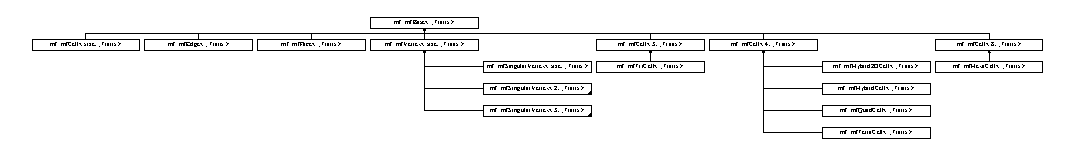
\includegraphics[height=1.630277cm]{classmf_1_1mfBase}
\end{center}
\end{figure}
\subsection*{Public Types}
\begin{DoxyCompactItemize}
\item 
typedef \_\-Traits::ids \hyperlink{classmf_1_1mfBase_a3b23f16ddf59da0a91ab12cf57c1f111}{ids}
\end{DoxyCompactItemize}
\subsection*{Public Member Functions}
\begin{DoxyCompactItemize}
\item 
\hyperlink{classmf_1_1mfBase_ad5f0db11c2b2936a128757870cf145a1}{mfBase} ()
\item 
virtual \hyperlink{classmf_1_1mfBase_a063c32e603a733ca7afdb080ffd160d3}{$\sim$mfBase} ()
\item 
bool \hyperlink{classmf_1_1mfBase_a11c27949a94ac6dc0f02a847e76fe7ed}{inMesh} (MF\_\-DMUTEXD)
\item 
void \hyperlink{classmf_1_1mfBase_aea06c4270e0a8b8509be3701f5579dd7}{setInMesh} (bool value MF\_\-DMUTEXVD)
\item 
void \hyperlink{classmf_1_1mfBase_ae092bf3cfdd2d57523418ed2f4cf1863}{setPosition} (\hyperlink{classmf_1_1mfBase_a3b23f16ddf59da0a91ab12cf57c1f111}{ids} position MF\_\-DMUTEXVD)
\item 
\hyperlink{classmf_1_1mfBase_a3b23f16ddf59da0a91ab12cf57c1f111}{ids} \hyperlink{classmf_1_1mfBase_af23d718a27ea598b23a33be5d372485e}{getPosition} (MF\_\-DMUTEXD)
\end{DoxyCompactItemize}
\subsection*{Protected Attributes}
\begin{DoxyCompactItemize}
\item 
MF\_\-FLAGS\_\-TYPE \hyperlink{classmf_1_1mfBase_a3551780d0be3b33270adbb3726d6e2d9}{flags}
\end{DoxyCompactItemize}
\subsubsection*{template$<$class \_\-Traits$>$ class mf::mfBase$<$ \_\-Traits $>$}



\subsection{Member Typedef Documentation}
\hypertarget{classmf_1_1mfBase_a3b23f16ddf59da0a91ab12cf57c1f111}{
\index{mf::mfBase@{mf::mfBase}!ids@{ids}}
\index{ids@{ids}!mf::mfBase@{mf::mfBase}}
\subsubsection[{ids}]{\setlength{\rightskip}{0pt plus 5cm}template$<$class \_\-Traits $>$ typedef \_\-Traits::ids {\bf mf::mfBase}$<$ \_\-Traits $>$::{\bf ids}}}
\label{classmf_1_1mfBase_a3b23f16ddf59da0a91ab12cf57c1f111}
Id typename definition 

Reimplemented in \hyperlink{classmf_1_1mfCell_a9e32102899fb1e6b5e95b08a6c71063f}{mf::mfCell$<$ size, \_\-Traits $>$}, \hyperlink{classmf_1_1mfHexaCell_a0f1d3a8aa5b31635f48c2d1baa1a9f37}{mf::mfHexaCell$<$ \_\-Traits $>$}, \hyperlink{classmf_1_1mfHybrid2DCell_a0ee11399531818ab7eac9c5fede19b14}{mf::mfHybrid2DCell$<$ \_\-Traits $>$}, \hyperlink{classmf_1_1mfHybridCell_afcc1603f9fd31f5e82fc0f2175aa74d2}{mf::mfHybridCell$<$ \_\-Traits $>$}, \hyperlink{classmf_1_1mfQuadCell_a443cbcdcefb50bddded8078d38869040}{mf::mfQuadCell$<$ \_\-Traits $>$}, \hyperlink{classmf_1_1mfSingularVertex_ad951601375961980e2ad033de57e14a1}{mf::mfSingularVertex$<$ size, \_\-Traits $>$}, \hyperlink{classmf_1_1mfTetraCell_a1fe27f9bfd856ec3464b2b671ceaf558}{mf::mfTetraCell$<$ \_\-Traits $>$}, \hyperlink{classmf_1_1mfTriCell_ae8b5f3ec0b85289a7f8b39e1869458e4}{mf::mfTriCell$<$ \_\-Traits $>$}, \hyperlink{classmf_1_1mfCell_a9e32102899fb1e6b5e95b08a6c71063f}{mf::mfCell$<$ 3, \_\-Traits $>$}, \hyperlink{classmf_1_1mfCell_a9e32102899fb1e6b5e95b08a6c71063f}{mf::mfCell$<$ 4, \_\-Traits $>$}, \hyperlink{classmf_1_1mfCell_a9e32102899fb1e6b5e95b08a6c71063f}{mf::mfCell$<$ 8, \_\-Traits $>$}, \hyperlink{classmf_1_1mfSingularVertex_ad951601375961980e2ad033de57e14a1}{mf::mfSingularVertex$<$ 2, \_\-Traits $>$}, and \hyperlink{classmf_1_1mfSingularVertex_ad951601375961980e2ad033de57e14a1}{mf::mfSingularVertex$<$ 3, \_\-Traits $>$}.



\subsection{Constructor \& Destructor Documentation}
\hypertarget{classmf_1_1mfBase_ad5f0db11c2b2936a128757870cf145a1}{
\index{mf::mfBase@{mf::mfBase}!mfBase@{mfBase}}
\index{mfBase@{mfBase}!mf::mfBase@{mf::mfBase}}
\subsubsection[{mfBase}]{\setlength{\rightskip}{0pt plus 5cm}template$<$class \_\-Traits $>$ {\bf mf::mfBase}$<$ \_\-Traits $>$::{\bf mfBase} (
\begin{DoxyParamCaption}
{}
\end{DoxyParamCaption}
)}}
\label{classmf_1_1mfBase_ad5f0db11c2b2936a128757870cf145a1}
Constructor

Initialize the mutex; Set this element as out of mesh \hypertarget{classmf_1_1mfBase_a063c32e603a733ca7afdb080ffd160d3}{
\index{mf::mfBase@{mf::mfBase}!$\sim$mfBase@{$\sim$mfBase}}
\index{$\sim$mfBase@{$\sim$mfBase}!mf::mfBase@{mf::mfBase}}
\subsubsection[{$\sim$mfBase}]{\setlength{\rightskip}{0pt plus 5cm}template$<$class \_\-Traits $>$ {\bf mf::mfBase}$<$ \_\-Traits $>$::$\sim${\bf mfBase} (
\begin{DoxyParamCaption}
{}
\end{DoxyParamCaption}
)\hspace{0.3cm}{\ttfamily  \mbox{[}virtual\mbox{]}}}}
\label{classmf_1_1mfBase_a063c32e603a733ca7afdb080ffd160d3}
Destructor

Destroy mutex 

\subsection{Member Function Documentation}
\hypertarget{classmf_1_1mfBase_af23d718a27ea598b23a33be5d372485e}{
\index{mf::mfBase@{mf::mfBase}!getPosition@{getPosition}}
\index{getPosition@{getPosition}!mf::mfBase@{mf::mfBase}}
\subsubsection[{getPosition}]{\setlength{\rightskip}{0pt plus 5cm}template$<$class \_\-Traits $>$ IDS {\bf mf::mfBase}$<$ \_\-Traits $>$::getPosition (
\begin{DoxyParamCaption}
\item[{MF\_\-DMUTEXD}]{}
\end{DoxyParamCaption}
)}}
\label{classmf_1_1mfBase_af23d718a27ea598b23a33be5d372485e}
Get the next free element

\begin{DoxyReturn}{Returns}
Return the next free element, if was not define, returned value is negative. 
\end{DoxyReturn}
\hypertarget{classmf_1_1mfBase_a11c27949a94ac6dc0f02a847e76fe7ed}{
\index{mf::mfBase@{mf::mfBase}!inMesh@{inMesh}}
\index{inMesh@{inMesh}!mf::mfBase@{mf::mfBase}}
\subsubsection[{inMesh}]{\setlength{\rightskip}{0pt plus 5cm}template$<$class \_\-Traits $>$ bool {\bf mf::mfBase}$<$ \_\-Traits $>$::inMesh (
\begin{DoxyParamCaption}
\item[{MF\_\-DMUTEXD}]{}
\end{DoxyParamCaption}
)}}
\label{classmf_1_1mfBase_a11c27949a94ac6dc0f02a847e76fe7ed}
Check if this element is in mesh

\begin{DoxyReturn}{Returns}
true, if this element is in mesh 
\end{DoxyReturn}
\hypertarget{classmf_1_1mfBase_aea06c4270e0a8b8509be3701f5579dd7}{
\index{mf::mfBase@{mf::mfBase}!setInMesh@{setInMesh}}
\index{setInMesh@{setInMesh}!mf::mfBase@{mf::mfBase}}
\subsubsection[{setInMesh}]{\setlength{\rightskip}{0pt plus 5cm}template$<$class \_\-Traits $>$ void {\bf mf::mfBase}$<$ \_\-Traits $>$::setInMesh (
\begin{DoxyParamCaption}
\item[{bool value}]{MF\_\-DMUTEXVD}
\end{DoxyParamCaption}
)}}
\label{classmf_1_1mfBase_aea06c4270e0a8b8509be3701f5579dd7}
Set if this element is in mesh


\begin{DoxyParams}{Parameters}
{\em value,:} & the status of this element \\
\hline
\end{DoxyParams}
\hypertarget{classmf_1_1mfBase_ae092bf3cfdd2d57523418ed2f4cf1863}{
\index{mf::mfBase@{mf::mfBase}!setPosition@{setPosition}}
\index{setPosition@{setPosition}!mf::mfBase@{mf::mfBase}}
\subsubsection[{setPosition}]{\setlength{\rightskip}{0pt plus 5cm}template$<$class \_\-Traits $>$ void {\bf mf::mfBase}$<$ \_\-Traits $>$::setPosition (
\begin{DoxyParamCaption}
\item[{{\bf ids} position}]{MF\_\-DMUTEXVD}
\end{DoxyParamCaption}
)}}
\label{classmf_1_1mfBase_ae092bf3cfdd2d57523418ed2f4cf1863}
Set the next free element in vector

This position is stored in same place of flags


\begin{DoxyParams}{Parameters}
{\em position,:} & the index of next free position \\
\hline
\end{DoxyParams}


\subsection{Member Data Documentation}
\hypertarget{classmf_1_1mfBase_a3551780d0be3b33270adbb3726d6e2d9}{
\index{mf::mfBase@{mf::mfBase}!flags@{flags}}
\index{flags@{flags}!mf::mfBase@{mf::mfBase}}
\subsubsection[{flags}]{\setlength{\rightskip}{0pt plus 5cm}template$<$class \_\-Traits $>$ MF\_\-FLAGS\_\-TYPE {\bf mf::mfBase}$<$ \_\-Traits $>$::{\bf flags}\hspace{0.3cm}{\ttfamily  \mbox{[}protected\mbox{]}}}}
\label{classmf_1_1mfBase_a3551780d0be3b33270adbb3726d6e2d9}
Flag type definition 

The documentation for this class was generated from the following file:\begin{DoxyCompactItemize}
\item 
\hyperlink{mfBase_8h}{mfBase.h}\end{DoxyCompactItemize}

\hypertarget{classmf_1_1mfBinaryIO}{
\section{mf::mfBinaryIO$<$ \_\-Traits $>$ Class Template Reference}
\label{classmf_1_1mfBinaryIO}\index{mf::mfBinaryIO@{mf::mfBinaryIO}}
}
\subsection*{Public Types}
\begin{DoxyCompactItemize}
\item 
typedef \_\-Traits::space \hyperlink{classmf_1_1mfBinaryIO_a90e373b679656da911855f0f855f8dc8}{space}
\item 
typedef \_\-Traits::ids \hyperlink{classmf_1_1mfBinaryIO_a2e229a9a1a64191bfe2bda80a9328714}{ids}
\end{DoxyCompactItemize}
\subsection*{Public Member Functions}
\begin{DoxyCompactItemize}
\item 
\hyperlink{classmf_1_1mfBinaryIO_aa9f709f13c77d6bd68dd47fa94eab10d}{mfBinaryIO} ()
\item 
\hyperlink{classmf_1_1mfBinaryIO_a78f8441d13f96990a219026e53fe23a5}{$\sim$mfBinaryIO} ()
\item 
\hypertarget{classmf_1_1mfBinaryIO_a57738ff8f339dd322aee5afc15bb28c9}{
void {\bfseries idsStore} (ofstream \&fp, \hyperlink{classmf_1_1mfBinaryIO_a2e229a9a1a64191bfe2bda80a9328714}{ids} num)}
\label{classmf_1_1mfBinaryIO_a57738ff8f339dd322aee5afc15bb28c9}

\item 
\hypertarget{classmf_1_1mfBinaryIO_a6d8e8e0a30cff9cf1157162ef67944eb}{
\hyperlink{classmf_1_1mfBinaryIO_a2e229a9a1a64191bfe2bda80a9328714}{ids} {\bfseries idsLoad} (ifstream \&fp)}
\label{classmf_1_1mfBinaryIO_a6d8e8e0a30cff9cf1157162ef67944eb}

\item 
\hypertarget{classmf_1_1mfBinaryIO_a7761f8e596d29208644a41646a9e05a9}{
void {\bfseries spaceStore} (ofstream \&fp, \hyperlink{classmf_1_1mfBinaryIO_a90e373b679656da911855f0f855f8dc8}{space} num)}
\label{classmf_1_1mfBinaryIO_a7761f8e596d29208644a41646a9e05a9}

\item 
\hypertarget{classmf_1_1mfBinaryIO_a7b12da467f9e18e1b7858ff26de79a63}{
\hyperlink{classmf_1_1mfBinaryIO_a90e373b679656da911855f0f855f8dc8}{space} {\bfseries spaceLoad} (ifstream \&fp)}
\label{classmf_1_1mfBinaryIO_a7b12da467f9e18e1b7858ff26de79a63}

\end{DoxyCompactItemize}
\subsubsection*{template$<$class \_\-Traits$>$ class mf::mfBinaryIO$<$ \_\-Traits $>$}



\subsection{Member Typedef Documentation}
\hypertarget{classmf_1_1mfBinaryIO_a2e229a9a1a64191bfe2bda80a9328714}{
\index{mf::mfBinaryIO@{mf::mfBinaryIO}!ids@{ids}}
\index{ids@{ids}!mf::mfBinaryIO@{mf::mfBinaryIO}}
\subsubsection[{ids}]{\setlength{\rightskip}{0pt plus 5cm}template$<$class \_\-Traits $>$ typedef \_\-Traits::ids {\bf mf::mfBinaryIO}$<$ \_\-Traits $>$::{\bf ids}}}
\label{classmf_1_1mfBinaryIO_a2e229a9a1a64191bfe2bda80a9328714}
Id typename definition \hypertarget{classmf_1_1mfBinaryIO_a90e373b679656da911855f0f855f8dc8}{
\index{mf::mfBinaryIO@{mf::mfBinaryIO}!space@{space}}
\index{space@{space}!mf::mfBinaryIO@{mf::mfBinaryIO}}
\subsubsection[{space}]{\setlength{\rightskip}{0pt plus 5cm}template$<$class \_\-Traits $>$ typedef \_\-Traits::space {\bf mf::mfBinaryIO}$<$ \_\-Traits $>$::{\bf space}}}
\label{classmf_1_1mfBinaryIO_a90e373b679656da911855f0f855f8dc8}
Space typename definition 

\subsection{Constructor \& Destructor Documentation}
\hypertarget{classmf_1_1mfBinaryIO_aa9f709f13c77d6bd68dd47fa94eab10d}{
\index{mf::mfBinaryIO@{mf::mfBinaryIO}!mfBinaryIO@{mfBinaryIO}}
\index{mfBinaryIO@{mfBinaryIO}!mf::mfBinaryIO@{mf::mfBinaryIO}}
\subsubsection[{mfBinaryIO}]{\setlength{\rightskip}{0pt plus 5cm}template$<$class \_\-Traits $>$ {\bf mf::mfBinaryIO}$<$ \_\-Traits $>$::{\bf mfBinaryIO} (
\begin{DoxyParamCaption}
{}
\end{DoxyParamCaption}
)}}
\label{classmf_1_1mfBinaryIO_aa9f709f13c77d6bd68dd47fa94eab10d}
Constructor \hypertarget{classmf_1_1mfBinaryIO_a78f8441d13f96990a219026e53fe23a5}{
\index{mf::mfBinaryIO@{mf::mfBinaryIO}!$\sim$mfBinaryIO@{$\sim$mfBinaryIO}}
\index{$\sim$mfBinaryIO@{$\sim$mfBinaryIO}!mf::mfBinaryIO@{mf::mfBinaryIO}}
\subsubsection[{$\sim$mfBinaryIO}]{\setlength{\rightskip}{0pt plus 5cm}template$<$class \_\-Traits $>$ {\bf mf::mfBinaryIO}$<$ \_\-Traits $>$::$\sim${\bf mfBinaryIO} (
\begin{DoxyParamCaption}
{}
\end{DoxyParamCaption}
)}}
\label{classmf_1_1mfBinaryIO_a78f8441d13f96990a219026e53fe23a5}
Destructor 

The documentation for this class was generated from the following file:\begin{DoxyCompactItemize}
\item 
mfBinaryIO.h\end{DoxyCompactItemize}

\hypertarget{classmf_1_1mfBoundaryCellCIterator2D}{
\section{mf::mfBoundaryCellCIterator2D$<$ \_\-Traits $>$ Class Template Reference}
\label{classmf_1_1mfBoundaryCellCIterator2D}\index{mf::mfBoundaryCellCIterator2D@{mf::mfBoundaryCellCIterator2D}}
}
Inheritance diagram for mf::mfBoundaryCellCIterator2D$<$ \_\-Traits $>$:\begin{figure}[H]
\begin{center}
\leavevmode
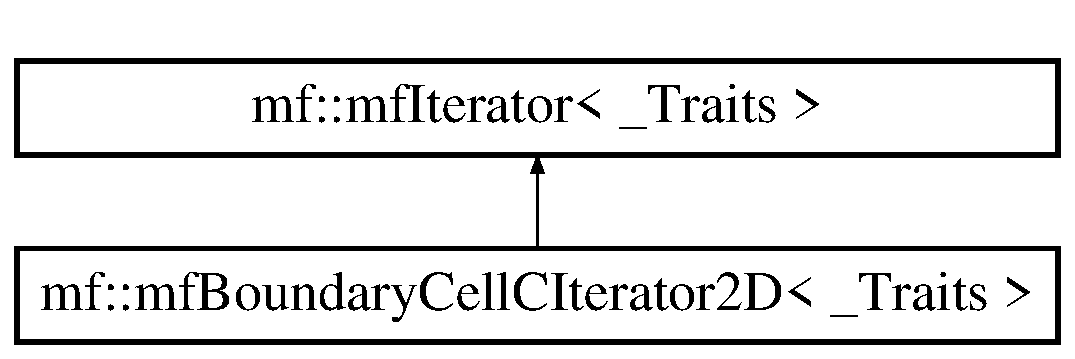
\includegraphics[height=2.000000cm]{classmf_1_1mfBoundaryCellCIterator2D}
\end{center}
\end{figure}
\subsection*{Public Types}
\begin{DoxyCompactItemize}
\item 
typedef \_\-Traits::sCell \hyperlink{classmf_1_1mfBoundaryCellCIterator2D_a0932e77a4d182a0c8a376b8ba1026e11}{sCell}
\item 
typedef \_\-Traits::ids \hyperlink{classmf_1_1mfBoundaryCellCIterator2D_a7b3c67238a3b4186e08f6fa05c11db31}{ids}
\item 
typedef \_\-Traits::sMesh \hyperlink{classmf_1_1mfBoundaryCellCIterator2D_a7cd4a533656715c1768db299fbd3e738}{sMesh}
\end{DoxyCompactItemize}
\subsection*{Public Member Functions}
\begin{DoxyCompactItemize}
\item 
\hyperlink{classmf_1_1mfBoundaryCellCIterator2D_ac598456518a9528acb750f02b0be0e1b}{mfBoundaryCellCIterator2D} (\hyperlink{classmf_1_1mfBoundaryCellCIterator2D_a7cd4a533656715c1768db299fbd3e738}{sMesh} $\ast$\_\-mesh)
\item 
\hyperlink{classmf_1_1mfBoundaryCellCIterator2D_a807ca41765b9d781cadcfa393e8809f5}{$\sim$mfBoundaryCellCIterator2D} ()
\item 
\hypertarget{classmf_1_1mfBoundaryCellCIterator2D_af62474764ead8b8ab90db13ea34e0b3e}{
bool {\bfseries initialize} (\hyperlink{classmf_1_1mfBoundaryCellCIterator2D_a7b3c67238a3b4186e08f6fa05c11db31}{ids} init, int edge=-\/1)}
\label{classmf_1_1mfBoundaryCellCIterator2D_af62474764ead8b8ab90db13ea34e0b3e}

\item 
\hypertarget{classmf_1_1mfBoundaryCellCIterator2D_adb5528bdca19812e17bb8f6fd77b6f0c}{
bool {\bfseries finish} ()}
\label{classmf_1_1mfBoundaryCellCIterator2D_adb5528bdca19812e17bb8f6fd77b6f0c}

\item 
\hypertarget{classmf_1_1mfBoundaryCellCIterator2D_ae4d022dc4bf3c9097574924e09cc4054}{
bool {\bfseries notFinish} ()}
\label{classmf_1_1mfBoundaryCellCIterator2D_ae4d022dc4bf3c9097574924e09cc4054}

\item 
\hypertarget{classmf_1_1mfBoundaryCellCIterator2D_ae6a922624356da41bd70e7bd57ba4f9c}{
bool {\bfseries operator++} ()}
\label{classmf_1_1mfBoundaryCellCIterator2D_ae6a922624356da41bd70e7bd57ba4f9c}

\item 
\hypertarget{classmf_1_1mfBoundaryCellCIterator2D_a3710326114e1799a5bdc517df26dba64}{
bool {\bfseries operator-\/-\/} ()}
\label{classmf_1_1mfBoundaryCellCIterator2D_a3710326114e1799a5bdc517df26dba64}

\item 
\hypertarget{classmf_1_1mfBoundaryCellCIterator2D_a88efc031c0f491998b92555c85c5bdac}{
\hyperlink{classmf_1_1mfBoundaryCellCIterator2D_a0932e77a4d182a0c8a376b8ba1026e11}{sCell} $\ast$ {\bfseries operator-\/$>$} ()}
\label{classmf_1_1mfBoundaryCellCIterator2D_a88efc031c0f491998b92555c85c5bdac}

\item 
\hypertarget{classmf_1_1mfBoundaryCellCIterator2D_a5f6aa7f86716791b8e723ca69bbc03a1}{
\hyperlink{classmf_1_1mfBoundaryCellCIterator2D_a0932e77a4d182a0c8a376b8ba1026e11}{sCell} $\ast$ {\bfseries operator$\ast$} ()}
\label{classmf_1_1mfBoundaryCellCIterator2D_a5f6aa7f86716791b8e723ca69bbc03a1}

\item 
\hypertarget{classmf_1_1mfBoundaryCellCIterator2D_aeb7e2b342eba8ed848a8579f2d529616}{
\hyperlink{classmf_1_1mfBoundaryCellCIterator2D_a7b3c67238a3b4186e08f6fa05c11db31}{ids} {\bfseries operator\&} ()}
\label{classmf_1_1mfBoundaryCellCIterator2D_aeb7e2b342eba8ed848a8579f2d529616}

\item 
\hypertarget{classmf_1_1mfBoundaryCellCIterator2D_a775d40179222a9f2764893c5843df0ad}{
int {\bfseries getEdge} ()}
\label{classmf_1_1mfBoundaryCellCIterator2D_a775d40179222a9f2764893c5843df0ad}

\end{DoxyCompactItemize}
\subsubsection*{template$<$class \_\-Traits$>$ class mf::mfBoundaryCellCIterator2D$<$ \_\-Traits $>$}



\subsection{Member Typedef Documentation}
\hypertarget{classmf_1_1mfBoundaryCellCIterator2D_a7b3c67238a3b4186e08f6fa05c11db31}{
\index{mf::mfBoundaryCellCIterator2D@{mf::mfBoundaryCellCIterator2D}!ids@{ids}}
\index{ids@{ids}!mf::mfBoundaryCellCIterator2D@{mf::mfBoundaryCellCIterator2D}}
\subsubsection[{ids}]{\setlength{\rightskip}{0pt plus 5cm}template$<$class \_\-Traits $>$ typedef \_\-Traits::ids {\bf mf::mfBoundaryCellCIterator2D}$<$ \_\-Traits $>$::{\bf ids}}}
\label{classmf_1_1mfBoundaryCellCIterator2D_a7b3c67238a3b4186e08f6fa05c11db31}
Id typename definition \hypertarget{classmf_1_1mfBoundaryCellCIterator2D_a0932e77a4d182a0c8a376b8ba1026e11}{
\index{mf::mfBoundaryCellCIterator2D@{mf::mfBoundaryCellCIterator2D}!sCell@{sCell}}
\index{sCell@{sCell}!mf::mfBoundaryCellCIterator2D@{mf::mfBoundaryCellCIterator2D}}
\subsubsection[{sCell}]{\setlength{\rightskip}{0pt plus 5cm}template$<$class \_\-Traits $>$ typedef \_\-Traits::sCell {\bf mf::mfBoundaryCellCIterator2D}$<$ \_\-Traits $>$::{\bf sCell}}}
\label{classmf_1_1mfBoundaryCellCIterator2D_a0932e77a4d182a0c8a376b8ba1026e11}
Cell typename definition \hypertarget{classmf_1_1mfBoundaryCellCIterator2D_a7cd4a533656715c1768db299fbd3e738}{
\index{mf::mfBoundaryCellCIterator2D@{mf::mfBoundaryCellCIterator2D}!sMesh@{sMesh}}
\index{sMesh@{sMesh}!mf::mfBoundaryCellCIterator2D@{mf::mfBoundaryCellCIterator2D}}
\subsubsection[{sMesh}]{\setlength{\rightskip}{0pt plus 5cm}template$<$class \_\-Traits $>$ typedef \_\-Traits::sMesh {\bf mf::mfBoundaryCellCIterator2D}$<$ \_\-Traits $>$::{\bf sMesh}}}
\label{classmf_1_1mfBoundaryCellCIterator2D_a7cd4a533656715c1768db299fbd3e738}
Mesh typename definition 

Reimplemented from \hyperlink{classmf_1_1mfIterator_aca31e4d7e7eca4e3b100530d8725064b}{mf::mfIterator$<$ \_\-Traits $>$}.



\subsection{Constructor \& Destructor Documentation}
\hypertarget{classmf_1_1mfBoundaryCellCIterator2D_ac598456518a9528acb750f02b0be0e1b}{
\index{mf::mfBoundaryCellCIterator2D@{mf::mfBoundaryCellCIterator2D}!mfBoundaryCellCIterator2D@{mfBoundaryCellCIterator2D}}
\index{mfBoundaryCellCIterator2D@{mfBoundaryCellCIterator2D}!mf::mfBoundaryCellCIterator2D@{mf::mfBoundaryCellCIterator2D}}
\subsubsection[{mfBoundaryCellCIterator2D}]{\setlength{\rightskip}{0pt plus 5cm}template$<$class \_\-Traits $>$ {\bf mf::mfBoundaryCellCIterator2D}$<$ \_\-Traits $>$::{\bf mfBoundaryCellCIterator2D} (
\begin{DoxyParamCaption}
\item[{{\bf sMesh} $\ast$}]{\_\-mesh}
\end{DoxyParamCaption}
)}}
\label{classmf_1_1mfBoundaryCellCIterator2D_ac598456518a9528acb750f02b0be0e1b}
Construtor \hypertarget{classmf_1_1mfBoundaryCellCIterator2D_a807ca41765b9d781cadcfa393e8809f5}{
\index{mf::mfBoundaryCellCIterator2D@{mf::mfBoundaryCellCIterator2D}!$\sim$mfBoundaryCellCIterator2D@{$\sim$mfBoundaryCellCIterator2D}}
\index{$\sim$mfBoundaryCellCIterator2D@{$\sim$mfBoundaryCellCIterator2D}!mf::mfBoundaryCellCIterator2D@{mf::mfBoundaryCellCIterator2D}}
\subsubsection[{$\sim$mfBoundaryCellCIterator2D}]{\setlength{\rightskip}{0pt plus 5cm}template$<$class \_\-Traits $>$ {\bf mf::mfBoundaryCellCIterator2D}$<$ \_\-Traits $>$::$\sim${\bf mfBoundaryCellCIterator2D} (
\begin{DoxyParamCaption}
{}
\end{DoxyParamCaption}
)}}
\label{classmf_1_1mfBoundaryCellCIterator2D_a807ca41765b9d781cadcfa393e8809f5}
Destrutor 

The documentation for this class was generated from the following file:\begin{DoxyCompactItemize}
\item 
mfBoundaryCellCIterator2D.h\end{DoxyCompactItemize}

\hypertarget{classmf_1_1mfBoundaryCellIterator2D}{
\section{mf::mfBoundaryCellIterator2D$<$ \_\-Traits $>$ Class Template Reference}
\label{classmf_1_1mfBoundaryCellIterator2D}\index{mf::mfBoundaryCellIterator2D@{mf::mfBoundaryCellIterator2D}}
}
Inheritance diagram for mf::mfBoundaryCellIterator2D$<$ \_\-Traits $>$:\begin{figure}[H]
\begin{center}
\leavevmode
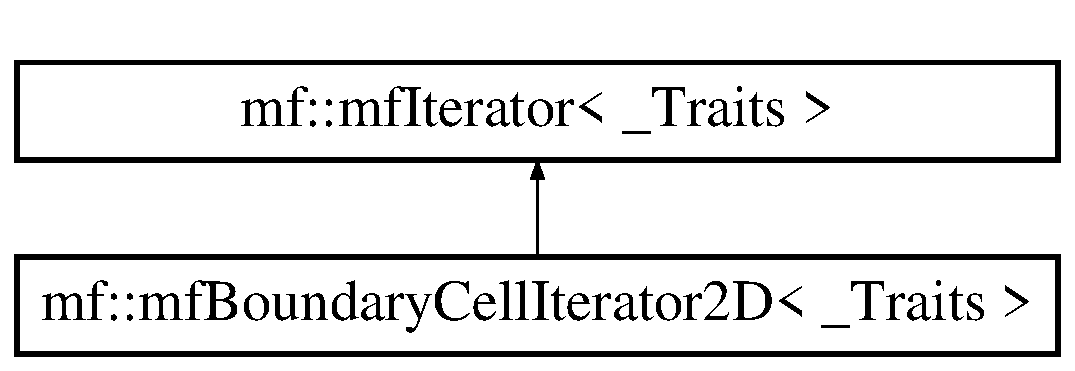
\includegraphics[height=2.000000cm]{classmf_1_1mfBoundaryCellIterator2D}
\end{center}
\end{figure}
\subsection*{Public Types}
\begin{DoxyCompactItemize}
\item 
typedef \_\-Traits::sCell \hyperlink{classmf_1_1mfBoundaryCellIterator2D_a3967d94a03a79073ae062491031e5339}{sCell}
\item 
typedef \_\-Traits::ids \hyperlink{classmf_1_1mfBoundaryCellIterator2D_ac315487c67a3604069747dc93ccb2fa0}{ids}
\item 
typedef \_\-Traits::sMesh \hyperlink{classmf_1_1mfBoundaryCellIterator2D_a4a2bc693e6241fee66020dd32ae7115e}{sMesh}
\end{DoxyCompactItemize}
\subsection*{Public Member Functions}
\begin{DoxyCompactItemize}
\item 
\hyperlink{classmf_1_1mfBoundaryCellIterator2D_a392e601a7ade40735e64a23d006ace5f}{mfBoundaryCellIterator2D} (\hyperlink{classmf_1_1mfBoundaryCellIterator2D_a4a2bc693e6241fee66020dd32ae7115e}{sMesh} $\ast$\_\-mesh)
\item 
\hyperlink{classmf_1_1mfBoundaryCellIterator2D_a6e7f77555a1d8247324e5ebc46b6c57c}{$\sim$mfBoundaryCellIterator2D} ()
\item 
\hypertarget{classmf_1_1mfBoundaryCellIterator2D_a8876c16e23d3ac379f04666dc12f0672}{
bool {\bfseries initialize} (\hyperlink{classmf_1_1mfBoundaryCellIterator2D_ac315487c67a3604069747dc93ccb2fa0}{ids} init, int edge=-\/1)}
\label{classmf_1_1mfBoundaryCellIterator2D_a8876c16e23d3ac379f04666dc12f0672}

\item 
\hypertarget{classmf_1_1mfBoundaryCellIterator2D_a5df9daba4d031502e09ace06305c1e50}{
bool {\bfseries finish} ()}
\label{classmf_1_1mfBoundaryCellIterator2D_a5df9daba4d031502e09ace06305c1e50}

\item 
\hypertarget{classmf_1_1mfBoundaryCellIterator2D_ab92476f50a181a11a00dcac956ed3823}{
bool {\bfseries notFinish} ()}
\label{classmf_1_1mfBoundaryCellIterator2D_ab92476f50a181a11a00dcac956ed3823}

\item 
\hypertarget{classmf_1_1mfBoundaryCellIterator2D_a233e76b9f2c7e21fe1335e3571991860}{
bool {\bfseries operator++} ()}
\label{classmf_1_1mfBoundaryCellIterator2D_a233e76b9f2c7e21fe1335e3571991860}

\item 
\hypertarget{classmf_1_1mfBoundaryCellIterator2D_a834b781ad2d94993f981df66eb3cca49}{
bool {\bfseries operator-\/-\/} ()}
\label{classmf_1_1mfBoundaryCellIterator2D_a834b781ad2d94993f981df66eb3cca49}

\item 
\hypertarget{classmf_1_1mfBoundaryCellIterator2D_a20b75e073d5af9a75dce7cb132489fc9}{
\hyperlink{classmf_1_1mfBoundaryCellIterator2D_a3967d94a03a79073ae062491031e5339}{sCell} $\ast$ {\bfseries operator-\/$>$} ()}
\label{classmf_1_1mfBoundaryCellIterator2D_a20b75e073d5af9a75dce7cb132489fc9}

\item 
\hypertarget{classmf_1_1mfBoundaryCellIterator2D_a416c04a9471359e6f4292143173b091a}{
\hyperlink{classmf_1_1mfBoundaryCellIterator2D_a3967d94a03a79073ae062491031e5339}{sCell} $\ast$ {\bfseries operator$\ast$} ()}
\label{classmf_1_1mfBoundaryCellIterator2D_a416c04a9471359e6f4292143173b091a}

\item 
\hypertarget{classmf_1_1mfBoundaryCellIterator2D_aae991485205ab0672814fcb24334abe7}{
\hyperlink{classmf_1_1mfBoundaryCellIterator2D_ac315487c67a3604069747dc93ccb2fa0}{ids} {\bfseries operator\&} ()}
\label{classmf_1_1mfBoundaryCellIterator2D_aae991485205ab0672814fcb24334abe7}

\item 
\hypertarget{classmf_1_1mfBoundaryCellIterator2D_a53aeb98ac0e8405f2d6961092bb67f50}{
int {\bfseries getEdge} ()}
\label{classmf_1_1mfBoundaryCellIterator2D_a53aeb98ac0e8405f2d6961092bb67f50}

\end{DoxyCompactItemize}
\subsubsection*{template$<$class \_\-Traits$>$ class mf::mfBoundaryCellIterator2D$<$ \_\-Traits $>$}



\subsection{Member Typedef Documentation}
\hypertarget{classmf_1_1mfBoundaryCellIterator2D_ac315487c67a3604069747dc93ccb2fa0}{
\index{mf::mfBoundaryCellIterator2D@{mf::mfBoundaryCellIterator2D}!ids@{ids}}
\index{ids@{ids}!mf::mfBoundaryCellIterator2D@{mf::mfBoundaryCellIterator2D}}
\subsubsection[{ids}]{\setlength{\rightskip}{0pt plus 5cm}template$<$class \_\-Traits $>$ typedef \_\-Traits::ids {\bf mf::mfBoundaryCellIterator2D}$<$ \_\-Traits $>$::{\bf ids}}}
\label{classmf_1_1mfBoundaryCellIterator2D_ac315487c67a3604069747dc93ccb2fa0}
Id typename definition \hypertarget{classmf_1_1mfBoundaryCellIterator2D_a3967d94a03a79073ae062491031e5339}{
\index{mf::mfBoundaryCellIterator2D@{mf::mfBoundaryCellIterator2D}!sCell@{sCell}}
\index{sCell@{sCell}!mf::mfBoundaryCellIterator2D@{mf::mfBoundaryCellIterator2D}}
\subsubsection[{sCell}]{\setlength{\rightskip}{0pt plus 5cm}template$<$class \_\-Traits $>$ typedef \_\-Traits::sCell {\bf mf::mfBoundaryCellIterator2D}$<$ \_\-Traits $>$::{\bf sCell}}}
\label{classmf_1_1mfBoundaryCellIterator2D_a3967d94a03a79073ae062491031e5339}
Cell typename definition \hypertarget{classmf_1_1mfBoundaryCellIterator2D_a4a2bc693e6241fee66020dd32ae7115e}{
\index{mf::mfBoundaryCellIterator2D@{mf::mfBoundaryCellIterator2D}!sMesh@{sMesh}}
\index{sMesh@{sMesh}!mf::mfBoundaryCellIterator2D@{mf::mfBoundaryCellIterator2D}}
\subsubsection[{sMesh}]{\setlength{\rightskip}{0pt plus 5cm}template$<$class \_\-Traits $>$ typedef \_\-Traits::sMesh {\bf mf::mfBoundaryCellIterator2D}$<$ \_\-Traits $>$::{\bf sMesh}}}
\label{classmf_1_1mfBoundaryCellIterator2D_a4a2bc693e6241fee66020dd32ae7115e}
Mesh typename definition 

Reimplemented from \hyperlink{classmf_1_1mfIterator_aca31e4d7e7eca4e3b100530d8725064b}{mf::mfIterator$<$ \_\-Traits $>$}.



\subsection{Constructor \& Destructor Documentation}
\hypertarget{classmf_1_1mfBoundaryCellIterator2D_a392e601a7ade40735e64a23d006ace5f}{
\index{mf::mfBoundaryCellIterator2D@{mf::mfBoundaryCellIterator2D}!mfBoundaryCellIterator2D@{mfBoundaryCellIterator2D}}
\index{mfBoundaryCellIterator2D@{mfBoundaryCellIterator2D}!mf::mfBoundaryCellIterator2D@{mf::mfBoundaryCellIterator2D}}
\subsubsection[{mfBoundaryCellIterator2D}]{\setlength{\rightskip}{0pt plus 5cm}template$<$class \_\-Traits $>$ {\bf mf::mfBoundaryCellIterator2D}$<$ \_\-Traits $>$::{\bf mfBoundaryCellIterator2D} (
\begin{DoxyParamCaption}
\item[{{\bf sMesh} $\ast$}]{\_\-mesh}
\end{DoxyParamCaption}
)}}
\label{classmf_1_1mfBoundaryCellIterator2D_a392e601a7ade40735e64a23d006ace5f}
Construtor \hypertarget{classmf_1_1mfBoundaryCellIterator2D_a6e7f77555a1d8247324e5ebc46b6c57c}{
\index{mf::mfBoundaryCellIterator2D@{mf::mfBoundaryCellIterator2D}!$\sim$mfBoundaryCellIterator2D@{$\sim$mfBoundaryCellIterator2D}}
\index{$\sim$mfBoundaryCellIterator2D@{$\sim$mfBoundaryCellIterator2D}!mf::mfBoundaryCellIterator2D@{mf::mfBoundaryCellIterator2D}}
\subsubsection[{$\sim$mfBoundaryCellIterator2D}]{\setlength{\rightskip}{0pt plus 5cm}template$<$class \_\-Traits $>$ {\bf mf::mfBoundaryCellIterator2D}$<$ \_\-Traits $>$::$\sim${\bf mfBoundaryCellIterator2D} (
\begin{DoxyParamCaption}
{}
\end{DoxyParamCaption}
)}}
\label{classmf_1_1mfBoundaryCellIterator2D_a6e7f77555a1d8247324e5ebc46b6c57c}
Destrutor 

The documentation for this class was generated from the following file:\begin{DoxyCompactItemize}
\item 
mfBoundaryCellIterator2D.h\end{DoxyCompactItemize}

\hypertarget{classmf_1_1mfCell}{
\section{mf::mfCell$<$ size, \_\-Traits $>$ Class Template Reference}
\label{classmf_1_1mfCell}\index{mf::mfCell@{mf::mfCell}}
}
Inheritance diagram for mf::mfCell$<$ size, \_\-Traits $>$:\begin{figure}[H]
\begin{center}
\leavevmode
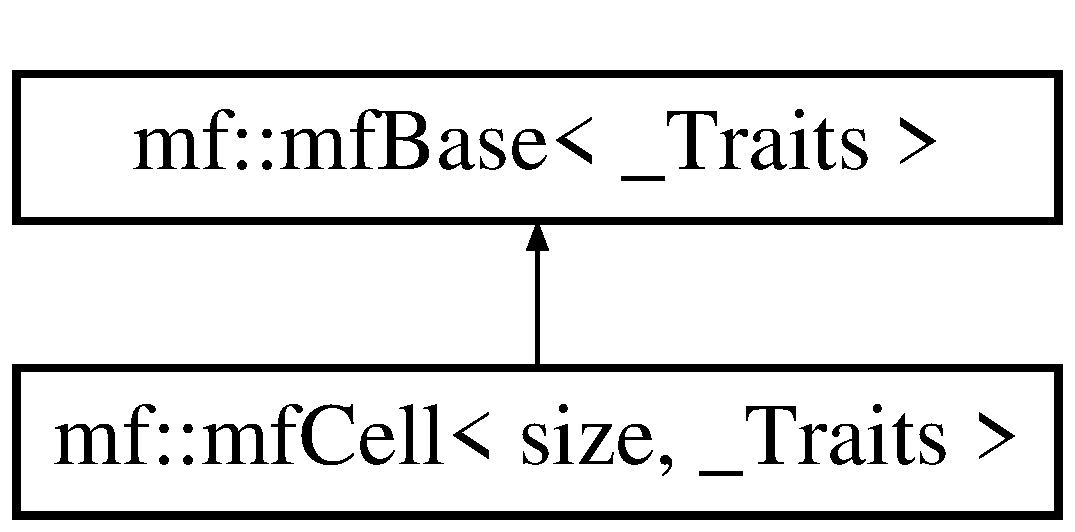
\includegraphics[height=2.000000cm]{classmf_1_1mfCell}
\end{center}
\end{figure}
\subsection*{Public Types}
\begin{DoxyCompactItemize}
\item 
typedef \_\-Traits::ids \hyperlink{classmf_1_1mfCell_a9e32102899fb1e6b5e95b08a6c71063f}{ids}
\end{DoxyCompactItemize}
\subsection*{Public Member Functions}
\begin{DoxyCompactItemize}
\item 
\hyperlink{classmf_1_1mfCell_a0a3e0565d5a6a6ec7d2c722311e4ac85}{mfCell} ()
\item 
virtual \hyperlink{classmf_1_1mfCell_aaaf2e41cb6328a63c4f4515fc2bc93ef}{$\sim$mfCell} ()
\item 
\hyperlink{classmf_1_1mfBase_a3b23f16ddf59da0a91ab12cf57c1f111}{ids} \hyperlink{classmf_1_1mfCell_a2c5d5cc9f5692d2802f86750c6e9c13f}{getMateId} (int index MF\_\-DMUTEXVD)
\item 
\hyperlink{classmf_1_1mfBase_a3b23f16ddf59da0a91ab12cf57c1f111}{ids} \hyperlink{classmf_1_1mfCell_ae207eaa3e7e4aa66fc6894781b12ab49}{getVertexId} (int index MF\_\-DMUTEXVD)
\item 
void \hyperlink{classmf_1_1mfCell_a96fe10c334f74928d220d46c3761f024}{setMateId} (int index, \hyperlink{classmf_1_1mfBase_a3b23f16ddf59da0a91ab12cf57c1f111}{ids} cell MF\_\-DMUTEXVD)
\item 
void \hyperlink{classmf_1_1mfCell_a79208565b35d445d4d1873d08021e37b}{setVertexId} (int index, \hyperlink{classmf_1_1mfBase_a3b23f16ddf59da0a91ab12cf57c1f111}{ids} vertex MF\_\-DMUTEXVD)
\item 
void \hyperlink{classmf_1_1mfCell_ac74f86234370beac5f821333ad1ceb4e}{clearMates} (MF\_\-DMUTEXD)
\item 
int \hyperlink{classmf_1_1mfCell_a0d82f1103c7674516156d27d35ac9186}{getVertexIndex} (\hyperlink{classmf_1_1mfBase_a3b23f16ddf59da0a91ab12cf57c1f111}{ids} vertex MF\_\-DMUTEXVD)
\item 
int \hyperlink{classmf_1_1mfCell_ae41581511f86555eaa0ebfb5581f55ea}{getMateIndex} (\hyperlink{classmf_1_1mfBase_a3b23f16ddf59da0a91ab12cf57c1f111}{ids} cell MF\_\-DMUTEXVD)
\item 
\hyperlink{classmf_1_1mfBase_a3b23f16ddf59da0a91ab12cf57c1f111}{ids} \hyperlink{classmf_1_1mfCell_a9c977b126d6f1dc12848c303be0c36b0}{getMateVertexId} (\hyperlink{classmf_1_1mfBase_a3b23f16ddf59da0a91ab12cf57c1f111}{ids} vertex MF\_\-DMUTEXVD)
\item 
\hyperlink{classmf_1_1mfBase_a3b23f16ddf59da0a91ab12cf57c1f111}{ids} \hyperlink{classmf_1_1mfCell_a120ea26866f9a71cced4b3256cfd63df}{getVertexMateId} (\hyperlink{classmf_1_1mfBase_a3b23f16ddf59da0a91ab12cf57c1f111}{ids} cell MF\_\-DMUTEXVD)
\end{DoxyCompactItemize}
\subsection*{Static Public Member Functions}
\begin{DoxyCompactItemize}
\item 
static int \hyperlink{classmf_1_1mfCell_adca6e1707e9d8487c22b3cd0117791a0}{getDimension} ()
\item 
static int \hyperlink{classmf_1_1mfCell_ae5031384bc660f1a804ab6603b8c1a19}{getNumberVerticesInCell} ()
\item 
static int \hyperlink{classmf_1_1mfCell_a16cc93bf1fa21c95014d000c9750e4a0}{getNumberEdgesInCell} ()
\end{DoxyCompactItemize}
\subsection*{Protected Attributes}
\begin{DoxyCompactItemize}
\item 
\hyperlink{classmf_1_1mfBase_a3b23f16ddf59da0a91ab12cf57c1f111}{ids} \hyperlink{classmf_1_1mfCell_a4d540b27089268665e1800cb7bf6b04d}{vertices} \mbox{[}size\mbox{]}
\item 
\hyperlink{classmf_1_1mfBase_a3b23f16ddf59da0a91ab12cf57c1f111}{ids} \hyperlink{classmf_1_1mfCell_a4bc12b8877d6ade93549032c569bb40f}{mates} \mbox{[}size\mbox{]}
\end{DoxyCompactItemize}
\subsubsection*{template$<$int size, class \_\-Traits$>$ class mf::mfCell$<$ size, \_\-Traits $>$}



\subsection{Member Typedef Documentation}
\hypertarget{classmf_1_1mfCell_a9e32102899fb1e6b5e95b08a6c71063f}{
\index{mf::mfCell@{mf::mfCell}!ids@{ids}}
\index{ids@{ids}!mf::mfCell@{mf::mfCell}}
\subsubsection[{ids}]{\setlength{\rightskip}{0pt plus 5cm}template$<$int size, class \_\-Traits$>$ typedef \_\-Traits::ids {\bf mf::mfCell}$<$ size, \_\-Traits $>$::{\bf ids}}}
\label{classmf_1_1mfCell_a9e32102899fb1e6b5e95b08a6c71063f}
Id typename definition 

Reimplemented from \hyperlink{classmf_1_1mfBase_a3b23f16ddf59da0a91ab12cf57c1f111}{mf::mfBase$<$ \_\-Traits $>$}.



Reimplemented in \hyperlink{classmf_1_1mfHexaCell_a0f1d3a8aa5b31635f48c2d1baa1a9f37}{mf::mfHexaCell$<$ \_\-Traits $>$}, \hyperlink{classmf_1_1mfHybrid2DCell_a0ee11399531818ab7eac9c5fede19b14}{mf::mfHybrid2DCell$<$ \_\-Traits $>$}, \hyperlink{classmf_1_1mfHybridCell_afcc1603f9fd31f5e82fc0f2175aa74d2}{mf::mfHybridCell$<$ \_\-Traits $>$}, \hyperlink{classmf_1_1mfQuadCell_a443cbcdcefb50bddded8078d38869040}{mf::mfQuadCell$<$ \_\-Traits $>$}, \hyperlink{classmf_1_1mfTetraCell_a1fe27f9bfd856ec3464b2b671ceaf558}{mf::mfTetraCell$<$ \_\-Traits $>$}, and \hyperlink{classmf_1_1mfTriCell_ae8b5f3ec0b85289a7f8b39e1869458e4}{mf::mfTriCell$<$ \_\-Traits $>$}.



\subsection{Constructor \& Destructor Documentation}
\hypertarget{classmf_1_1mfCell_a0a3e0565d5a6a6ec7d2c722311e4ac85}{
\index{mf::mfCell@{mf::mfCell}!mfCell@{mfCell}}
\index{mfCell@{mfCell}!mf::mfCell@{mf::mfCell}}
\subsubsection[{mfCell}]{\setlength{\rightskip}{0pt plus 5cm}template$<$int size, class \_\-Traits $>$ {\bf mf::mfCell}$<$ size, \_\-Traits $>$::{\bf mfCell} (
\begin{DoxyParamCaption}
{}
\end{DoxyParamCaption}
)}}
\label{classmf_1_1mfCell_a0a3e0565d5a6a6ec7d2c722311e4ac85}
Constructor

Initialize vertices and mates ids \hypertarget{classmf_1_1mfCell_aaaf2e41cb6328a63c4f4515fc2bc93ef}{
\index{mf::mfCell@{mf::mfCell}!$\sim$mfCell@{$\sim$mfCell}}
\index{$\sim$mfCell@{$\sim$mfCell}!mf::mfCell@{mf::mfCell}}
\subsubsection[{$\sim$mfCell}]{\setlength{\rightskip}{0pt plus 5cm}template$<$int size, class \_\-Traits $>$ {\bf mf::mfCell}$<$ size, \_\-Traits $>$::$\sim${\bf mfCell} (
\begin{DoxyParamCaption}
{}
\end{DoxyParamCaption}
)\hspace{0.3cm}{\ttfamily  \mbox{[}virtual\mbox{]}}}}
\label{classmf_1_1mfCell_aaaf2e41cb6328a63c4f4515fc2bc93ef}
Destructor 

\subsection{Member Function Documentation}
\hypertarget{classmf_1_1mfCell_ac74f86234370beac5f821333ad1ceb4e}{
\index{mf::mfCell@{mf::mfCell}!clearMates@{clearMates}}
\index{clearMates@{clearMates}!mf::mfCell@{mf::mfCell}}
\subsubsection[{clearMates}]{\setlength{\rightskip}{0pt plus 5cm}template$<$int size, class \_\-Traits$>$ void {\bf mf::mfCell}$<$ size, \_\-Traits $>$::clearMates (
\begin{DoxyParamCaption}
\item[{MF\_\-DMUTEXD}]{}
\end{DoxyParamCaption}
)}}
\label{classmf_1_1mfCell_ac74f86234370beac5f821333ad1ceb4e}
Reset the mate cells ids

(Defines -\/1 for all positions) 

Reimplemented in \hyperlink{classmf_1_1mfHexaCell_a924edba7b4baa1564851a09138c0d542}{mf::mfHexaCell$<$ \_\-Traits $>$}, and \hyperlink{classmf_1_1mfTetraCell_a9e553dc8c297b53756f44a9782facf5c}{mf::mfTetraCell$<$ \_\-Traits $>$}.

\hypertarget{classmf_1_1mfCell_adca6e1707e9d8487c22b3cd0117791a0}{
\index{mf::mfCell@{mf::mfCell}!getDimension@{getDimension}}
\index{getDimension@{getDimension}!mf::mfCell@{mf::mfCell}}
\subsubsection[{getDimension}]{\setlength{\rightskip}{0pt plus 5cm}template$<$int size, class \_\-Traits$>$ static int {\bf mf::mfCell}$<$ size, \_\-Traits $>$::getDimension (
\begin{DoxyParamCaption}
{}
\end{DoxyParamCaption}
)\hspace{0.3cm}{\ttfamily  \mbox{[}inline, static\mbox{]}}}}
\label{classmf_1_1mfCell_adca6e1707e9d8487c22b3cd0117791a0}
Return the dimension of this cell 

Reimplemented in \hyperlink{classmf_1_1mfHexaCell_ab53eff357bcacf391a82031240993a32}{mf::mfHexaCell$<$ \_\-Traits $>$}, \hyperlink{classmf_1_1mfHybrid2DCell_a93668aada55d3779cfadd32c068eb5e2}{mf::mfHybrid2DCell$<$ \_\-Traits $>$}, \hyperlink{classmf_1_1mfHybridCell_a4fb353f76e3fd38febcf2f71c1e11d76}{mf::mfHybridCell$<$ \_\-Traits $>$}, \hyperlink{classmf_1_1mfQuadCell_a797da8c9839219488be115b41d9ebe6b}{mf::mfQuadCell$<$ \_\-Traits $>$}, and \hyperlink{classmf_1_1mfTetraCell_a6934653e054673d25dbb1bd8bddbc453}{mf::mfTetraCell$<$ \_\-Traits $>$}.

\hypertarget{classmf_1_1mfCell_a2c5d5cc9f5692d2802f86750c6e9c13f}{
\index{mf::mfCell@{mf::mfCell}!getMateId@{getMateId}}
\index{getMateId@{getMateId}!mf::mfCell@{mf::mfCell}}
\subsubsection[{getMateId}]{\setlength{\rightskip}{0pt plus 5cm}template$<$int size, class \_\-Traits $>$ IDS {\bf mf::mfCell}$<$ size, \_\-Traits $>$::getMateId (
\begin{DoxyParamCaption}
\item[{int index}]{MF\_\-DMUTEXVD}
\end{DoxyParamCaption}
)}}
\label{classmf_1_1mfCell_a2c5d5cc9f5692d2802f86750c6e9c13f}
Return the mate cell id of the specified index


\begin{DoxyParams}{Parameters}
{\em index,:} & position of mate cell \\
\hline
\end{DoxyParams}
\begin{DoxyReturn}{Returns}
mate cell id. 
\end{DoxyReturn}


Reimplemented in \hyperlink{classmf_1_1mfHexaCell_a42fa61d5e21e646e99c905d20792b9c8}{mf::mfHexaCell$<$ \_\-Traits $>$}, and \hyperlink{classmf_1_1mfTetraCell_a946fd7394f718ef614076d3a15314b07}{mf::mfTetraCell$<$ \_\-Traits $>$}.

\hypertarget{classmf_1_1mfCell_ae41581511f86555eaa0ebfb5581f55ea}{
\index{mf::mfCell@{mf::mfCell}!getMateIndex@{getMateIndex}}
\index{getMateIndex@{getMateIndex}!mf::mfCell@{mf::mfCell}}
\subsubsection[{getMateIndex}]{\setlength{\rightskip}{0pt plus 5cm}template$<$int size, class \_\-Traits $>$ int {\bf mf::mfCell}$<$ size, \_\-Traits $>$::getMateIndex (
\begin{DoxyParamCaption}
\item[{{\bf ids} cell}]{MF\_\-DMUTEXVD}
\end{DoxyParamCaption}
)}}
\label{classmf_1_1mfCell_ae41581511f86555eaa0ebfb5581f55ea}
Return the position/index (in the cell) of the specified mate cell id


\begin{DoxyParams}{Parameters}
{\em cell,:} & the mate cell id \\
\hline
\end{DoxyParams}
\begin{DoxyReturn}{Returns}
the mate index. 
\end{DoxyReturn}


Reimplemented in \hyperlink{classmf_1_1mfHexaCell_ae40ba149ff474250c814bf6c7f3af415}{mf::mfHexaCell$<$ \_\-Traits $>$}, and \hyperlink{classmf_1_1mfTetraCell_a6fb6c0adb551ec4bbefe01c4e71ec443}{mf::mfTetraCell$<$ \_\-Traits $>$}.

\hypertarget{classmf_1_1mfCell_a9c977b126d6f1dc12848c303be0c36b0}{
\index{mf::mfCell@{mf::mfCell}!getMateVertexId@{getMateVertexId}}
\index{getMateVertexId@{getMateVertexId}!mf::mfCell@{mf::mfCell}}
\subsubsection[{getMateVertexId}]{\setlength{\rightskip}{0pt plus 5cm}template$<$int size, class \_\-Traits $>$ IDS {\bf mf::mfCell}$<$ size, \_\-Traits $>$::getMateVertexId (
\begin{DoxyParamCaption}
\item[{{\bf ids} vertex}]{MF\_\-DMUTEXVD}
\end{DoxyParamCaption}
)}}
\label{classmf_1_1mfCell_a9c977b126d6f1dc12848c303be0c36b0}
Return the opposite cell id of the specified vertex id. To be used only in surface meshes


\begin{DoxyParams}{Parameters}
{\em cell,:} & the vertex id \\
\hline
\end{DoxyParams}
\begin{DoxyReturn}{Returns}
mate cell id. 
\end{DoxyReturn}


Reimplemented in \hyperlink{classmf_1_1mfTetraCell_a0e5f9859616dfa35c3409fa5649c195c}{mf::mfTetraCell$<$ \_\-Traits $>$}.

\hypertarget{classmf_1_1mfCell_a16cc93bf1fa21c95014d000c9750e4a0}{
\index{mf::mfCell@{mf::mfCell}!getNumberEdgesInCell@{getNumberEdgesInCell}}
\index{getNumberEdgesInCell@{getNumberEdgesInCell}!mf::mfCell@{mf::mfCell}}
\subsubsection[{getNumberEdgesInCell}]{\setlength{\rightskip}{0pt plus 5cm}template$<$int size, class \_\-Traits$>$ static int {\bf mf::mfCell}$<$ size, \_\-Traits $>$::getNumberEdgesInCell (
\begin{DoxyParamCaption}
{}
\end{DoxyParamCaption}
)\hspace{0.3cm}{\ttfamily  \mbox{[}inline, static\mbox{]}}}}
\label{classmf_1_1mfCell_a16cc93bf1fa21c95014d000c9750e4a0}
Return the number of edges of this cell 

Reimplemented in \hyperlink{classmf_1_1mfHexaCell_a34bda59c389b7e9228fbeb6dadac27c3}{mf::mfHexaCell$<$ \_\-Traits $>$}, \hyperlink{classmf_1_1mfHybrid2DCell_a717323295b1a993d0c9d029978c84743}{mf::mfHybrid2DCell$<$ \_\-Traits $>$}, \hyperlink{classmf_1_1mfHybridCell_a5fc9ef1bea17984822cf28d0ed6dde20}{mf::mfHybridCell$<$ \_\-Traits $>$}, and \hyperlink{classmf_1_1mfTetraCell_a49b7f454b739781a34fb4fa7152b66ac}{mf::mfTetraCell$<$ \_\-Traits $>$}.

\hypertarget{classmf_1_1mfCell_ae5031384bc660f1a804ab6603b8c1a19}{
\index{mf::mfCell@{mf::mfCell}!getNumberVerticesInCell@{getNumberVerticesInCell}}
\index{getNumberVerticesInCell@{getNumberVerticesInCell}!mf::mfCell@{mf::mfCell}}
\subsubsection[{getNumberVerticesInCell}]{\setlength{\rightskip}{0pt plus 5cm}template$<$int size, class \_\-Traits$>$ static int {\bf mf::mfCell}$<$ size, \_\-Traits $>$::getNumberVerticesInCell (
\begin{DoxyParamCaption}
{}
\end{DoxyParamCaption}
)\hspace{0.3cm}{\ttfamily  \mbox{[}inline, static\mbox{]}}}}
\label{classmf_1_1mfCell_ae5031384bc660f1a804ab6603b8c1a19}
Return the number of vertices of this cell 

Reimplemented in \hyperlink{classmf_1_1mfHexaCell_a734a620daad4302ebda00686bcb8bd96}{mf::mfHexaCell$<$ \_\-Traits $>$}, \hyperlink{classmf_1_1mfHybrid2DCell_a0d49a5d889459f5100357c45d192d179}{mf::mfHybrid2DCell$<$ \_\-Traits $>$}, \hyperlink{classmf_1_1mfHybridCell_a39449ac79227d63f7cf505305ceb89d0}{mf::mfHybridCell$<$ \_\-Traits $>$}, and \hyperlink{classmf_1_1mfTetraCell_a6a49b05e337c5aef4647acef176a8bf7}{mf::mfTetraCell$<$ \_\-Traits $>$}.

\hypertarget{classmf_1_1mfCell_ae207eaa3e7e4aa66fc6894781b12ab49}{
\index{mf::mfCell@{mf::mfCell}!getVertexId@{getVertexId}}
\index{getVertexId@{getVertexId}!mf::mfCell@{mf::mfCell}}
\subsubsection[{getVertexId}]{\setlength{\rightskip}{0pt plus 5cm}template$<$int size, class \_\-Traits $>$ IDS {\bf mf::mfCell}$<$ size, \_\-Traits $>$::getVertexId (
\begin{DoxyParamCaption}
\item[{int index}]{MF\_\-DMUTEXVD}
\end{DoxyParamCaption}
)}}
\label{classmf_1_1mfCell_ae207eaa3e7e4aa66fc6894781b12ab49}
Return the vertex id of the specified index


\begin{DoxyParams}{Parameters}
{\em index,:} & position of vertex \\
\hline
\end{DoxyParams}
\begin{DoxyReturn}{Returns}
the vertex id. 
\end{DoxyReturn}
\hypertarget{classmf_1_1mfCell_a0d82f1103c7674516156d27d35ac9186}{
\index{mf::mfCell@{mf::mfCell}!getVertexIndex@{getVertexIndex}}
\index{getVertexIndex@{getVertexIndex}!mf::mfCell@{mf::mfCell}}
\subsubsection[{getVertexIndex}]{\setlength{\rightskip}{0pt plus 5cm}template$<$int size, class \_\-Traits $>$ int {\bf mf::mfCell}$<$ size, \_\-Traits $>$::getVertexIndex (
\begin{DoxyParamCaption}
\item[{{\bf ids} vertex}]{MF\_\-DMUTEXVD}
\end{DoxyParamCaption}
)}}
\label{classmf_1_1mfCell_a0d82f1103c7674516156d27d35ac9186}
Return the position/index (in the cell) of the specified vertex id


\begin{DoxyParams}{Parameters}
{\em vertex,:} & the vertex id \\
\hline
\end{DoxyParams}
\begin{DoxyReturn}{Returns}
the vertex index. 
\end{DoxyReturn}
\hypertarget{classmf_1_1mfCell_a120ea26866f9a71cced4b3256cfd63df}{
\index{mf::mfCell@{mf::mfCell}!getVertexMateId@{getVertexMateId}}
\index{getVertexMateId@{getVertexMateId}!mf::mfCell@{mf::mfCell}}
\subsubsection[{getVertexMateId}]{\setlength{\rightskip}{0pt plus 5cm}template$<$int size, class \_\-Traits $>$ IDS {\bf mf::mfCell}$<$ size, \_\-Traits $>$::getVertexMateId (
\begin{DoxyParamCaption}
\item[{{\bf ids} cell}]{MF\_\-DMUTEXVD}
\end{DoxyParamCaption}
)}}
\label{classmf_1_1mfCell_a120ea26866f9a71cced4b3256cfd63df}
Return the opposite vertex id of the specified mate cell id


\begin{DoxyParams}{Parameters}
{\em cell,:} & the mate cell id \\
\hline
\end{DoxyParams}


Reimplemented in \hyperlink{classmf_1_1mfTetraCell_aad9f514199dea3408d6a14d0bb1f9f97}{mf::mfTetraCell$<$ \_\-Traits $>$}.

\hypertarget{classmf_1_1mfCell_a96fe10c334f74928d220d46c3761f024}{
\index{mf::mfCell@{mf::mfCell}!setMateId@{setMateId}}
\index{setMateId@{setMateId}!mf::mfCell@{mf::mfCell}}
\subsubsection[{setMateId}]{\setlength{\rightskip}{0pt plus 5cm}template$<$int size, class \_\-Traits $>$ void {\bf mf::mfCell}$<$ size, \_\-Traits $>$::setMateId (
\begin{DoxyParamCaption}
\item[{int}]{index, }
\item[{{\bf ids} cell}]{MF\_\-DMUTEXVD}
\end{DoxyParamCaption}
)}}
\label{classmf_1_1mfCell_a96fe10c334f74928d220d46c3761f024}
Define the mate cell id of the specified index


\begin{DoxyParams}{Parameters}
{\em index,:} & position of mate cell \\
\hline
{\em cell,:} & the mate cell id \\
\hline
\end{DoxyParams}


Reimplemented in \hyperlink{classmf_1_1mfHexaCell_ab512173b13d97508d23083de414491e9}{mf::mfHexaCell$<$ \_\-Traits $>$}, and \hyperlink{classmf_1_1mfTetraCell_acbe15a78f605cfbbc8f62acc3cf4bc0a}{mf::mfTetraCell$<$ \_\-Traits $>$}.

\hypertarget{classmf_1_1mfCell_a79208565b35d445d4d1873d08021e37b}{
\index{mf::mfCell@{mf::mfCell}!setVertexId@{setVertexId}}
\index{setVertexId@{setVertexId}!mf::mfCell@{mf::mfCell}}
\subsubsection[{setVertexId}]{\setlength{\rightskip}{0pt plus 5cm}template$<$int size, class \_\-Traits $>$ void {\bf mf::mfCell}$<$ size, \_\-Traits $>$::setVertexId (
\begin{DoxyParamCaption}
\item[{int}]{index, }
\item[{{\bf ids} vertex}]{MF\_\-DMUTEXVD}
\end{DoxyParamCaption}
)}}
\label{classmf_1_1mfCell_a79208565b35d445d4d1873d08021e37b}
Define the vertex id of the specified index


\begin{DoxyParams}{Parameters}
{\em index,:} & position of vertex \\
\hline
{\em vertex,:} & the vertex id \\
\hline
\end{DoxyParams}


\subsection{Member Data Documentation}
\hypertarget{classmf_1_1mfCell_a4bc12b8877d6ade93549032c569bb40f}{
\index{mf::mfCell@{mf::mfCell}!mates@{mates}}
\index{mates@{mates}!mf::mfCell@{mf::mfCell}}
\subsubsection[{mates}]{\setlength{\rightskip}{0pt plus 5cm}template$<$int size, class \_\-Traits$>$ {\bf ids} {\bf mf::mfCell}$<$ size, \_\-Traits $>$::{\bf mates}\mbox{[}size\mbox{]}\hspace{0.3cm}{\ttfamily  \mbox{[}protected\mbox{]}}}}
\label{classmf_1_1mfCell_a4bc12b8877d6ade93549032c569bb40f}
Cell's mate cell ids, number of mates vary accordingly to the type of cell \hypertarget{classmf_1_1mfCell_a4d540b27089268665e1800cb7bf6b04d}{
\index{mf::mfCell@{mf::mfCell}!vertices@{vertices}}
\index{vertices@{vertices}!mf::mfCell@{mf::mfCell}}
\subsubsection[{vertices}]{\setlength{\rightskip}{0pt plus 5cm}template$<$int size, class \_\-Traits$>$ {\bf ids} {\bf mf::mfCell}$<$ size, \_\-Traits $>$::{\bf vertices}\mbox{[}size\mbox{]}\hspace{0.3cm}{\ttfamily  \mbox{[}protected\mbox{]}}}}
\label{classmf_1_1mfCell_a4d540b27089268665e1800cb7bf6b04d}
Cell's vertices ids, number of vertices vary accordingly to the type of cell 

The documentation for this class was generated from the following file:\begin{DoxyCompactItemize}
\item 
\hyperlink{mfCell_8h}{mfCell.h}\end{DoxyCompactItemize}

\hypertarget{classmf_1_1mfCellsIterator}{
\section{mf::mfCellsIterator$<$ \_\-Traits $>$ Class Template Reference}
\label{classmf_1_1mfCellsIterator}\index{mf::mfCellsIterator@{mf::mfCellsIterator}}
}
Inheritance diagram for mf::mfCellsIterator$<$ \_\-Traits $>$:\begin{figure}[H]
\begin{center}
\leavevmode
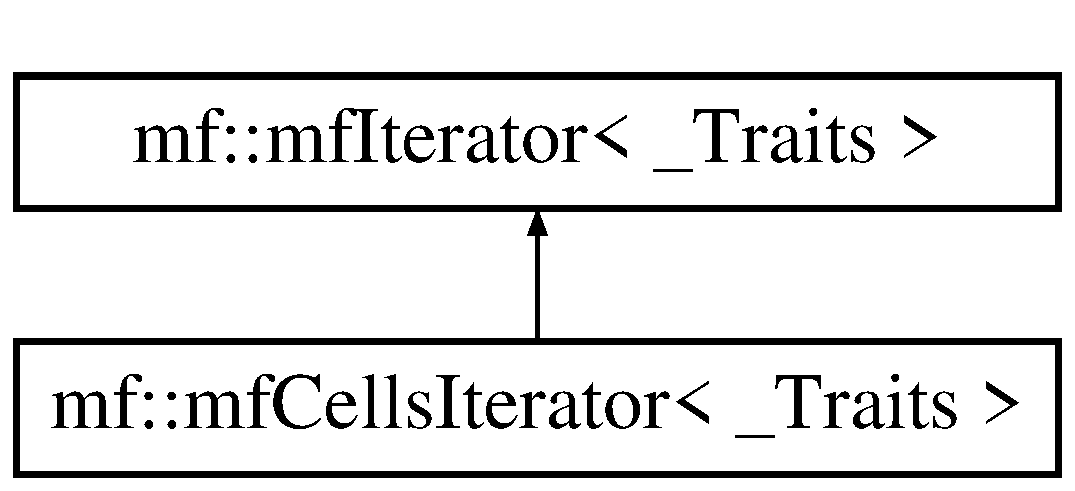
\includegraphics[height=2.000000cm]{classmf_1_1mfCellsIterator}
\end{center}
\end{figure}
\subsection*{Public Types}
\begin{DoxyCompactItemize}
\item 
typedef \_\-Traits::sCell \hyperlink{classmf_1_1mfCellsIterator_afe3e76ed6519e2ad74dff562b23aa52f}{sCell}
\item 
typedef \_\-Traits::ids \hyperlink{classmf_1_1mfCellsIterator_a836ea7a8c64a86f414d71c2556969e1c}{ids}
\item 
typedef \_\-Traits::sMesh \hyperlink{classmf_1_1mfCellsIterator_a3f16876b669a93e719af84cdc0c9dad9}{sMesh}
\end{DoxyCompactItemize}
\subsection*{Public Member Functions}
\begin{DoxyCompactItemize}
\item 
\hyperlink{classmf_1_1mfCellsIterator_a90f4c8266b67b81efbee9936bc7a842f}{mfCellsIterator} (\hyperlink{classmf_1_1mfCellsIterator_a3f16876b669a93e719af84cdc0c9dad9}{sMesh} $\ast$\_\-mesh)
\item 
\hyperlink{classmf_1_1mfCellsIterator_a6feca02d665106fb830fa17330f38590}{$\sim$mfCellsIterator} ()
\item 
\hypertarget{classmf_1_1mfCellsIterator_a4de3605d01d890c82feb0199404b121d}{
bool {\bfseries initialize} (\hyperlink{classmf_1_1mfCellsIterator_a836ea7a8c64a86f414d71c2556969e1c}{ids} init=0)}
\label{classmf_1_1mfCellsIterator_a4de3605d01d890c82feb0199404b121d}

\item 
\hypertarget{classmf_1_1mfCellsIterator_a29e11edaafdc4edb8d5ba7ce7e660726}{
bool {\bfseries finish} ()}
\label{classmf_1_1mfCellsIterator_a29e11edaafdc4edb8d5ba7ce7e660726}

\item 
\hypertarget{classmf_1_1mfCellsIterator_a6b68793cd767fdb0c14bcfe600dacf1f}{
bool {\bfseries notFinish} ()}
\label{classmf_1_1mfCellsIterator_a6b68793cd767fdb0c14bcfe600dacf1f}

\item 
\hypertarget{classmf_1_1mfCellsIterator_ae96bd545093a2fabf5416635dcdf4ec2}{
bool {\bfseries operator++} ()}
\label{classmf_1_1mfCellsIterator_ae96bd545093a2fabf5416635dcdf4ec2}

\item 
\hypertarget{classmf_1_1mfCellsIterator_a362a257218e710fccc9b2331271676dc}{
bool {\bfseries operator-\/-\/} ()}
\label{classmf_1_1mfCellsIterator_a362a257218e710fccc9b2331271676dc}

\item 
\hypertarget{classmf_1_1mfCellsIterator_ae842271166b868c31de3a9c42cfe8da1}{
\hyperlink{classmf_1_1mfCellsIterator_afe3e76ed6519e2ad74dff562b23aa52f}{sCell} $\ast$ {\bfseries operator-\/$>$} ()}
\label{classmf_1_1mfCellsIterator_ae842271166b868c31de3a9c42cfe8da1}

\item 
\hypertarget{classmf_1_1mfCellsIterator_a390b1a0472973355b4b29b25b6b7438d}{
\hyperlink{classmf_1_1mfCellsIterator_afe3e76ed6519e2ad74dff562b23aa52f}{sCell} $\ast$ {\bfseries operator$\ast$} ()}
\label{classmf_1_1mfCellsIterator_a390b1a0472973355b4b29b25b6b7438d}

\item 
\hypertarget{classmf_1_1mfCellsIterator_ab88ecf8ebf06b2347518183da3fc78e1}{
\hyperlink{classmf_1_1mfCellsIterator_a836ea7a8c64a86f414d71c2556969e1c}{ids} {\bfseries operator\&} ()}
\label{classmf_1_1mfCellsIterator_ab88ecf8ebf06b2347518183da3fc78e1}

\end{DoxyCompactItemize}
\subsubsection*{template$<$class \_\-Traits$>$ class mf::mfCellsIterator$<$ \_\-Traits $>$}



\subsection{Member Typedef Documentation}
\hypertarget{classmf_1_1mfCellsIterator_a836ea7a8c64a86f414d71c2556969e1c}{
\index{mf::mfCellsIterator@{mf::mfCellsIterator}!ids@{ids}}
\index{ids@{ids}!mf::mfCellsIterator@{mf::mfCellsIterator}}
\subsubsection[{ids}]{\setlength{\rightskip}{0pt plus 5cm}template$<$class \_\-Traits $>$ typedef \_\-Traits::ids {\bf mf::mfCellsIterator}$<$ \_\-Traits $>$::{\bf ids}}}
\label{classmf_1_1mfCellsIterator_a836ea7a8c64a86f414d71c2556969e1c}
Id typename definition \hypertarget{classmf_1_1mfCellsIterator_afe3e76ed6519e2ad74dff562b23aa52f}{
\index{mf::mfCellsIterator@{mf::mfCellsIterator}!sCell@{sCell}}
\index{sCell@{sCell}!mf::mfCellsIterator@{mf::mfCellsIterator}}
\subsubsection[{sCell}]{\setlength{\rightskip}{0pt plus 5cm}template$<$class \_\-Traits $>$ typedef \_\-Traits::sCell {\bf mf::mfCellsIterator}$<$ \_\-Traits $>$::{\bf sCell}}}
\label{classmf_1_1mfCellsIterator_afe3e76ed6519e2ad74dff562b23aa52f}
Cell typename definition \hypertarget{classmf_1_1mfCellsIterator_a3f16876b669a93e719af84cdc0c9dad9}{
\index{mf::mfCellsIterator@{mf::mfCellsIterator}!sMesh@{sMesh}}
\index{sMesh@{sMesh}!mf::mfCellsIterator@{mf::mfCellsIterator}}
\subsubsection[{sMesh}]{\setlength{\rightskip}{0pt plus 5cm}template$<$class \_\-Traits $>$ typedef \_\-Traits::sMesh {\bf mf::mfCellsIterator}$<$ \_\-Traits $>$::{\bf sMesh}}}
\label{classmf_1_1mfCellsIterator_a3f16876b669a93e719af84cdc0c9dad9}
Mesh typename definition 

Reimplemented from \hyperlink{classmf_1_1mfIterator_aca31e4d7e7eca4e3b100530d8725064b}{mf::mfIterator$<$ \_\-Traits $>$}.



\subsection{Constructor \& Destructor Documentation}
\hypertarget{classmf_1_1mfCellsIterator_a90f4c8266b67b81efbee9936bc7a842f}{
\index{mf::mfCellsIterator@{mf::mfCellsIterator}!mfCellsIterator@{mfCellsIterator}}
\index{mfCellsIterator@{mfCellsIterator}!mf::mfCellsIterator@{mf::mfCellsIterator}}
\subsubsection[{mfCellsIterator}]{\setlength{\rightskip}{0pt plus 5cm}template$<$class \_\-Traits $>$ {\bf mf::mfCellsIterator}$<$ \_\-Traits $>$::{\bf mfCellsIterator} (
\begin{DoxyParamCaption}
\item[{{\bf sMesh} $\ast$}]{\_\-mesh}
\end{DoxyParamCaption}
)}}
\label{classmf_1_1mfCellsIterator_a90f4c8266b67b81efbee9936bc7a842f}
Constructor \hypertarget{classmf_1_1mfCellsIterator_a6feca02d665106fb830fa17330f38590}{
\index{mf::mfCellsIterator@{mf::mfCellsIterator}!$\sim$mfCellsIterator@{$\sim$mfCellsIterator}}
\index{$\sim$mfCellsIterator@{$\sim$mfCellsIterator}!mf::mfCellsIterator@{mf::mfCellsIterator}}
\subsubsection[{$\sim$mfCellsIterator}]{\setlength{\rightskip}{0pt plus 5cm}template$<$class \_\-Traits $>$ {\bf mf::mfCellsIterator}$<$ \_\-Traits $>$::$\sim${\bf mfCellsIterator} (
\begin{DoxyParamCaption}
{}
\end{DoxyParamCaption}
)}}
\label{classmf_1_1mfCellsIterator_a6feca02d665106fb830fa17330f38590}
Destructor 

The documentation for this class was generated from the following file:\begin{DoxyCompactItemize}
\item 
\hyperlink{mfCellsIterator_8h}{mfCellsIterator.h}\end{DoxyCompactItemize}

\hypertarget{structmf_1_1mfDefault2D}{
\section{mf::mfDefault2D Struct Reference}
\label{structmf_1_1mfDefault2D}\index{mf::mfDefault2D@{mf::mfDefault2D}}
}


{\ttfamily \#include $<$mfTraits.h$>$}

\subsection*{Public Types}
\begin{DoxyCompactItemize}
\item 
typedef \hyperlink{structmf_1_1mfDefault2D}{mfDefault2D} \hyperlink{structmf_1_1mfDefault2D_a8139211f36d360a0221d3a8e8221bbce}{sTraits}
\item 
typedef double \hyperlink{structmf_1_1mfDefault2D_adb9cddf677f4712bef5bfcb90f64d2f9}{space}
\item 
typedef int \hyperlink{structmf_1_1mfDefault2D_a0c23cfe375bcd646eed0501ca539127d}{ids}
\item 
typedef \hyperlink{classmf_1_1mfVertex2D}{mfVertex2D}$<$ \hyperlink{structmf_1_1mfDefault2D}{sTraits} $>$ \hyperlink{structmf_1_1mfDefault2D_a427f10d57187e5fe16a2b3ae91d18ea2}{sVertex}
\item 
typedef \hyperlink{classmf_1_1mfEdge}{mfEdge}$<$ \hyperlink{structmf_1_1mfDefault2D}{sTraits} $>$ \hyperlink{structmf_1_1mfDefault2D_aee1699c9233b1e9b0461258cda97dd95}{sEdge}
\item 
typedef \hyperlink{classmf_1_1mfTriCell}{mfTriCell}$<$ \hyperlink{structmf_1_1mfDefault2D}{sTraits} $>$ \hyperlink{structmf_1_1mfDefault2D_a00494a3737ff059da660e6b2448d85e7}{sCell}
\item 
typedef \hyperlink{classmf_1_1mfMesh}{mfMesh}$<$ \hyperlink{structmf_1_1mfDefault2D}{sTraits} $>$ \hyperlink{structmf_1_1mfDefault2D_a8d813cb3f2395cfcfeaa8bd4f9c5eade}{sMesh}
\item 
typedef \hyperlink{classmf_1_1mfMesh2D}{mfMesh2D}$<$ \hyperlink{structmf_1_1mfDefault2D}{sTraits} $>$ \hyperlink{structmf_1_1mfDefault2D_a62b4225279579e884393a540e2e628cb}{sOper}
\item 
typedef \hyperlink{classmf_1_1mfGeometric}{mfGeometric}$<$ \hyperlink{structmf_1_1mfDefault2D}{sTraits} $>$ \hyperlink{structmf_1_1mfDefault2D_a974a8a9297a6c7dbe28a3aae93ec0932}{sGeometric}
\item 
typedef \hyperlink{classmf_1_1mfTopology}{mfTopology}$<$ \hyperlink{structmf_1_1mfDefault2D}{sTraits} $>$ \hyperlink{structmf_1_1mfDefault2D_aa4faa97e437f812f5bad578e7862ce0f}{sTopology}
\end{DoxyCompactItemize}


\subsection{Detailed Description}
Defines the features of a default 2D triangular mesh 

\subsection{Member Typedef Documentation}
\hypertarget{structmf_1_1mfDefault2D_a0c23cfe375bcd646eed0501ca539127d}{
\index{mf::mfDefault2D@{mf::mfDefault2D}!ids@{ids}}
\index{ids@{ids}!mf::mfDefault2D@{mf::mfDefault2D}}
\subsubsection[{ids}]{\setlength{\rightskip}{0pt plus 5cm}typedef int {\bf mf::mfDefault2D::ids}}}
\label{structmf_1_1mfDefault2D_a0c23cfe375bcd646eed0501ca539127d}
Id type definition \hypertarget{structmf_1_1mfDefault2D_a00494a3737ff059da660e6b2448d85e7}{
\index{mf::mfDefault2D@{mf::mfDefault2D}!sCell@{sCell}}
\index{sCell@{sCell}!mf::mfDefault2D@{mf::mfDefault2D}}
\subsubsection[{sCell}]{\setlength{\rightskip}{0pt plus 5cm}typedef {\bf mfTriCell}$<${\bf sTraits}$>$ {\bf mf::mfDefault2D::sCell}}}
\label{structmf_1_1mfDefault2D_a00494a3737ff059da660e6b2448d85e7}
Triangular cell definition \hypertarget{structmf_1_1mfDefault2D_aee1699c9233b1e9b0461258cda97dd95}{
\index{mf::mfDefault2D@{mf::mfDefault2D}!sEdge@{sEdge}}
\index{sEdge@{sEdge}!mf::mfDefault2D@{mf::mfDefault2D}}
\subsubsection[{sEdge}]{\setlength{\rightskip}{0pt plus 5cm}typedef {\bf mfEdge}$<${\bf sTraits}$>$ {\bf mf::mfDefault2D::sEdge}}}
\label{structmf_1_1mfDefault2D_aee1699c9233b1e9b0461258cda97dd95}
Edge definition \hypertarget{structmf_1_1mfDefault2D_a974a8a9297a6c7dbe28a3aae93ec0932}{
\index{mf::mfDefault2D@{mf::mfDefault2D}!sGeometric@{sGeometric}}
\index{sGeometric@{sGeometric}!mf::mfDefault2D@{mf::mfDefault2D}}
\subsubsection[{sGeometric}]{\setlength{\rightskip}{0pt plus 5cm}typedef {\bf mfGeometric}$<${\bf sTraits}$>$ {\bf mf::mfDefault2D::sGeometric}}}
\label{structmf_1_1mfDefault2D_a974a8a9297a6c7dbe28a3aae93ec0932}
Geometric operations class definition \hypertarget{structmf_1_1mfDefault2D_a8d813cb3f2395cfcfeaa8bd4f9c5eade}{
\index{mf::mfDefault2D@{mf::mfDefault2D}!sMesh@{sMesh}}
\index{sMesh@{sMesh}!mf::mfDefault2D@{mf::mfDefault2D}}
\subsubsection[{sMesh}]{\setlength{\rightskip}{0pt plus 5cm}typedef {\bf mfMesh}$<${\bf sTraits}$>$ {\bf mf::mfDefault2D::sMesh}}}
\label{structmf_1_1mfDefault2D_a8d813cb3f2395cfcfeaa8bd4f9c5eade}
Mesh definition \hypertarget{structmf_1_1mfDefault2D_a62b4225279579e884393a540e2e628cb}{
\index{mf::mfDefault2D@{mf::mfDefault2D}!sOper@{sOper}}
\index{sOper@{sOper}!mf::mfDefault2D@{mf::mfDefault2D}}
\subsubsection[{sOper}]{\setlength{\rightskip}{0pt plus 5cm}typedef {\bf mfMesh2D}$<${\bf sTraits}$>$ {\bf mf::mfDefault2D::sOper}}}
\label{structmf_1_1mfDefault2D_a62b4225279579e884393a540e2e628cb}
2D mesh operation class definition \hypertarget{structmf_1_1mfDefault2D_adb9cddf677f4712bef5bfcb90f64d2f9}{
\index{mf::mfDefault2D@{mf::mfDefault2D}!space@{space}}
\index{space@{space}!mf::mfDefault2D@{mf::mfDefault2D}}
\subsubsection[{space}]{\setlength{\rightskip}{0pt plus 5cm}typedef double {\bf mf::mfDefault2D::space}}}
\label{structmf_1_1mfDefault2D_adb9cddf677f4712bef5bfcb90f64d2f9}
Space type definition \hypertarget{structmf_1_1mfDefault2D_aa4faa97e437f812f5bad578e7862ce0f}{
\index{mf::mfDefault2D@{mf::mfDefault2D}!sTopology@{sTopology}}
\index{sTopology@{sTopology}!mf::mfDefault2D@{mf::mfDefault2D}}
\subsubsection[{sTopology}]{\setlength{\rightskip}{0pt plus 5cm}typedef {\bf mfTopology}$<${\bf sTraits}$>$ {\bf mf::mfDefault2D::sTopology}}}
\label{structmf_1_1mfDefault2D_aa4faa97e437f812f5bad578e7862ce0f}
Topological operations class definition \hypertarget{structmf_1_1mfDefault2D_a8139211f36d360a0221d3a8e8221bbce}{
\index{mf::mfDefault2D@{mf::mfDefault2D}!sTraits@{sTraits}}
\index{sTraits@{sTraits}!mf::mfDefault2D@{mf::mfDefault2D}}
\subsubsection[{sTraits}]{\setlength{\rightskip}{0pt plus 5cm}typedef {\bf mfDefault2D} {\bf mf::mfDefault2D::sTraits}}}
\label{structmf_1_1mfDefault2D_a8139211f36d360a0221d3a8e8221bbce}
Trait type definition \hypertarget{structmf_1_1mfDefault2D_a427f10d57187e5fe16a2b3ae91d18ea2}{
\index{mf::mfDefault2D@{mf::mfDefault2D}!sVertex@{sVertex}}
\index{sVertex@{sVertex}!mf::mfDefault2D@{mf::mfDefault2D}}
\subsubsection[{sVertex}]{\setlength{\rightskip}{0pt plus 5cm}typedef {\bf mfVertex2D}$<${\bf sTraits}$>$ {\bf mf::mfDefault2D::sVertex}}}
\label{structmf_1_1mfDefault2D_a427f10d57187e5fe16a2b3ae91d18ea2}
2D vertex definition 

The documentation for this struct was generated from the following file:\begin{DoxyCompactItemize}
\item 
mfTraits.h\end{DoxyCompactItemize}

\hypertarget{structmf_1_1mfDefaultHexahedra}{
\section{mf::mfDefaultHexahedra Struct Reference}
\label{structmf_1_1mfDefaultHexahedra}\index{mf::mfDefaultHexahedra@{mf::mfDefaultHexahedra}}
}


{\ttfamily \#include $<$mfTraits.h$>$}

\subsection*{Public Types}
\begin{DoxyCompactItemize}
\item 
typedef \hyperlink{structmf_1_1mfDefaultHexahedra}{mfDefaultHexahedra} \hyperlink{structmf_1_1mfDefaultHexahedra_a557747fd5ab6ee8bd28a0f1a3f201473}{sTraits}
\item 
typedef double \hyperlink{structmf_1_1mfDefaultHexahedra_a54662287a7b444574598fb0d18f027f3}{space}
\item 
typedef int \hyperlink{structmf_1_1mfDefaultHexahedra_a57a742de88b24adcba862c9333d2164a}{ids}
\item 
typedef \hyperlink{classmf_1_1mfVertex3D}{mfVertex3D}$<$ \hyperlink{structmf_1_1mfDefaultHexahedra}{sTraits} $>$ \hyperlink{structmf_1_1mfDefaultHexahedra_a3cc593a4024b66fb2bf899e4f650c784}{sVertex}
\item 
typedef \hyperlink{classmf_1_1mfEdge}{mfEdge}$<$ \hyperlink{structmf_1_1mfDefaultHexahedra}{sTraits} $>$ \hyperlink{structmf_1_1mfDefaultHexahedra_a344dd6b466e412c06a16151b4e366c04}{sEdge}
\item 
typedef \hyperlink{classmf_1_1mfHexaCell}{mfHexaCell}$<$ \hyperlink{structmf_1_1mfDefaultHexahedra}{sTraits} $>$ \hyperlink{structmf_1_1mfDefaultHexahedra_a8ec40ad2dedf7b88583df8f40007382e}{sCell}
\item 
typedef \hyperlink{classmf_1_1mfMesh}{mfMesh}$<$ \hyperlink{structmf_1_1mfDefaultHexahedra}{sTraits} $>$ \hyperlink{structmf_1_1mfDefaultHexahedra_a63486f47d4047cd32e139f19792d00b6}{sMesh}
\item 
typedef \hyperlink{classmf_1_1mfMeshHexa}{mfMeshHexa}$<$ \hyperlink{structmf_1_1mfDefaultHexahedra}{sTraits} $>$ \hyperlink{structmf_1_1mfDefaultHexahedra_a83be74be71b56f14d6041afa586196a2}{sOper}
\item 
typedef \hyperlink{classmf_1_1mfGeometric}{mfGeometric}$<$ \hyperlink{structmf_1_1mfDefaultHexahedra}{sTraits} $>$ \hyperlink{structmf_1_1mfDefaultHexahedra_a53ee4c731be21fc32670a7c8959febe5}{sGeometric}
\item 
typedef \hyperlink{classmf_1_1mfTopology}{mfTopology}$<$ \hyperlink{structmf_1_1mfDefaultHexahedra}{sTraits} $>$ \hyperlink{structmf_1_1mfDefaultHexahedra_a570a4ce963193f8414eeb0add001d0cb}{sTopology}
\end{DoxyCompactItemize}


\subsection{Detailed Description}
Defines the features of a default hexahedral mesh 

\subsection{Member Typedef Documentation}
\hypertarget{structmf_1_1mfDefaultHexahedra_a57a742de88b24adcba862c9333d2164a}{
\index{mf::mfDefaultHexahedra@{mf::mfDefaultHexahedra}!ids@{ids}}
\index{ids@{ids}!mf::mfDefaultHexahedra@{mf::mfDefaultHexahedra}}
\subsubsection[{ids}]{\setlength{\rightskip}{0pt plus 5cm}typedef int {\bf mf::mfDefaultHexahedra::ids}}}
\label{structmf_1_1mfDefaultHexahedra_a57a742de88b24adcba862c9333d2164a}
Id type definition \hypertarget{structmf_1_1mfDefaultHexahedra_a8ec40ad2dedf7b88583df8f40007382e}{
\index{mf::mfDefaultHexahedra@{mf::mfDefaultHexahedra}!sCell@{sCell}}
\index{sCell@{sCell}!mf::mfDefaultHexahedra@{mf::mfDefaultHexahedra}}
\subsubsection[{sCell}]{\setlength{\rightskip}{0pt plus 5cm}typedef {\bf mfHexaCell}$<${\bf sTraits}$>$ {\bf mf::mfDefaultHexahedra::sCell}}}
\label{structmf_1_1mfDefaultHexahedra_a8ec40ad2dedf7b88583df8f40007382e}
Hexahedral cell definition \hypertarget{structmf_1_1mfDefaultHexahedra_a344dd6b466e412c06a16151b4e366c04}{
\index{mf::mfDefaultHexahedra@{mf::mfDefaultHexahedra}!sEdge@{sEdge}}
\index{sEdge@{sEdge}!mf::mfDefaultHexahedra@{mf::mfDefaultHexahedra}}
\subsubsection[{sEdge}]{\setlength{\rightskip}{0pt plus 5cm}typedef {\bf mfEdge}$<${\bf sTraits}$>$ {\bf mf::mfDefaultHexahedra::sEdge}}}
\label{structmf_1_1mfDefaultHexahedra_a344dd6b466e412c06a16151b4e366c04}
Edge definition \hypertarget{structmf_1_1mfDefaultHexahedra_a53ee4c731be21fc32670a7c8959febe5}{
\index{mf::mfDefaultHexahedra@{mf::mfDefaultHexahedra}!sGeometric@{sGeometric}}
\index{sGeometric@{sGeometric}!mf::mfDefaultHexahedra@{mf::mfDefaultHexahedra}}
\subsubsection[{sGeometric}]{\setlength{\rightskip}{0pt plus 5cm}typedef {\bf mfGeometric}$<${\bf sTraits}$>$ {\bf mf::mfDefaultHexahedra::sGeometric}}}
\label{structmf_1_1mfDefaultHexahedra_a53ee4c731be21fc32670a7c8959febe5}
Geometric operations class definition \hypertarget{structmf_1_1mfDefaultHexahedra_a63486f47d4047cd32e139f19792d00b6}{
\index{mf::mfDefaultHexahedra@{mf::mfDefaultHexahedra}!sMesh@{sMesh}}
\index{sMesh@{sMesh}!mf::mfDefaultHexahedra@{mf::mfDefaultHexahedra}}
\subsubsection[{sMesh}]{\setlength{\rightskip}{0pt plus 5cm}typedef {\bf mfMesh}$<${\bf sTraits}$>$ {\bf mf::mfDefaultHexahedra::sMesh}}}
\label{structmf_1_1mfDefaultHexahedra_a63486f47d4047cd32e139f19792d00b6}
Mesh definition \hypertarget{structmf_1_1mfDefaultHexahedra_a83be74be71b56f14d6041afa586196a2}{
\index{mf::mfDefaultHexahedra@{mf::mfDefaultHexahedra}!sOper@{sOper}}
\index{sOper@{sOper}!mf::mfDefaultHexahedra@{mf::mfDefaultHexahedra}}
\subsubsection[{sOper}]{\setlength{\rightskip}{0pt plus 5cm}typedef {\bf mfMeshHexa}$<${\bf sTraits}$>$ {\bf mf::mfDefaultHexahedra::sOper}}}
\label{structmf_1_1mfDefaultHexahedra_a83be74be71b56f14d6041afa586196a2}
Volumetric mesh operation class definition \hypertarget{structmf_1_1mfDefaultHexahedra_a54662287a7b444574598fb0d18f027f3}{
\index{mf::mfDefaultHexahedra@{mf::mfDefaultHexahedra}!space@{space}}
\index{space@{space}!mf::mfDefaultHexahedra@{mf::mfDefaultHexahedra}}
\subsubsection[{space}]{\setlength{\rightskip}{0pt plus 5cm}typedef double {\bf mf::mfDefaultHexahedra::space}}}
\label{structmf_1_1mfDefaultHexahedra_a54662287a7b444574598fb0d18f027f3}
Space type definition \hypertarget{structmf_1_1mfDefaultHexahedra_a570a4ce963193f8414eeb0add001d0cb}{
\index{mf::mfDefaultHexahedra@{mf::mfDefaultHexahedra}!sTopology@{sTopology}}
\index{sTopology@{sTopology}!mf::mfDefaultHexahedra@{mf::mfDefaultHexahedra}}
\subsubsection[{sTopology}]{\setlength{\rightskip}{0pt plus 5cm}typedef {\bf mfTopology}$<${\bf sTraits}$>$ {\bf mf::mfDefaultHexahedra::sTopology}}}
\label{structmf_1_1mfDefaultHexahedra_a570a4ce963193f8414eeb0add001d0cb}
Topological operations class definition \hypertarget{structmf_1_1mfDefaultHexahedra_a557747fd5ab6ee8bd28a0f1a3f201473}{
\index{mf::mfDefaultHexahedra@{mf::mfDefaultHexahedra}!sTraits@{sTraits}}
\index{sTraits@{sTraits}!mf::mfDefaultHexahedra@{mf::mfDefaultHexahedra}}
\subsubsection[{sTraits}]{\setlength{\rightskip}{0pt plus 5cm}typedef {\bf mfDefaultHexahedra} {\bf mf::mfDefaultHexahedra::sTraits}}}
\label{structmf_1_1mfDefaultHexahedra_a557747fd5ab6ee8bd28a0f1a3f201473}
Trait type definition \hypertarget{structmf_1_1mfDefaultHexahedra_a3cc593a4024b66fb2bf899e4f650c784}{
\index{mf::mfDefaultHexahedra@{mf::mfDefaultHexahedra}!sVertex@{sVertex}}
\index{sVertex@{sVertex}!mf::mfDefaultHexahedra@{mf::mfDefaultHexahedra}}
\subsubsection[{sVertex}]{\setlength{\rightskip}{0pt plus 5cm}typedef {\bf mfVertex3D}$<${\bf sTraits}$>$ {\bf mf::mfDefaultHexahedra::sVertex}}}
\label{structmf_1_1mfDefaultHexahedra_a3cc593a4024b66fb2bf899e4f650c784}
3D vertex definition 

The documentation for this struct was generated from the following file:\begin{DoxyCompactItemize}
\item 
mfTraits.h\end{DoxyCompactItemize}

\hypertarget{structmf_1_1mfDefaultHybridSurface}{
\section{mf::mfDefaultHybridSurface Struct Reference}
\label{structmf_1_1mfDefaultHybridSurface}\index{mf::mfDefaultHybridSurface@{mf::mfDefaultHybridSurface}}
}


{\ttfamily \#include $<$mfTraits.h$>$}

\subsection*{Public Types}
\begin{DoxyCompactItemize}
\item 
typedef \hyperlink{structmf_1_1mfDefaultHybridSurface}{mfDefaultHybridSurface} \hyperlink{structmf_1_1mfDefaultHybridSurface_a6b7ae8a86c4047ca8a529515dc042449}{sTraits}
\item 
typedef double \hyperlink{structmf_1_1mfDefaultHybridSurface_aa60f8021d9313ec87752ef7c4909d2fa}{space}
\item 
typedef int \hyperlink{structmf_1_1mfDefaultHybridSurface_a06ff6d28f156383ae914862d15231cf6}{ids}
\item 
typedef \hyperlink{classmf_1_1mfVertex3D}{mfVertex3D}$<$ \hyperlink{structmf_1_1mfDefaultHybridSurface}{sTraits} $>$ \hyperlink{structmf_1_1mfDefaultHybridSurface_ad0362cd301479efd028b8e30d875332f}{sVertex}
\item 
typedef \hyperlink{classmf_1_1mfEdge}{mfEdge}$<$ \hyperlink{structmf_1_1mfDefaultHybridSurface}{sTraits} $>$ \hyperlink{structmf_1_1mfDefaultHybridSurface_a5c8e36a36a12cce1d11af275786101d8}{sEdge}
\item 
typedef \hyperlink{classmf_1_1mfHybrid2DCell}{mfHybrid2DCell}$<$ \hyperlink{structmf_1_1mfDefaultHybridSurface}{sTraits} $>$ \hyperlink{structmf_1_1mfDefaultHybridSurface_aba9244a2c4a635841589c4ff27b1eaaa}{sCell}
\item 
typedef \hyperlink{classmf_1_1mfMesh}{mfMesh}$<$ \hyperlink{structmf_1_1mfDefaultHybridSurface}{sTraits} $>$ \hyperlink{structmf_1_1mfDefaultHybridSurface_a3ef0c32e3cccb46dbc126f3d40ade56c}{sMesh}
\item 
typedef \hyperlink{classmf_1_1mfMeshHybridSurface}{mfMeshHybridSurface}$<$ \hyperlink{structmf_1_1mfDefaultHybridSurface}{sTraits} $>$ \hyperlink{structmf_1_1mfDefaultHybridSurface_a048af8fc38cf0f61cb53c72431bdf589}{sOper}
\item 
typedef \hyperlink{classmf_1_1mfGeometric}{mfGeometric}$<$ \hyperlink{structmf_1_1mfDefaultHybridSurface}{sTraits} $>$ \hyperlink{structmf_1_1mfDefaultHybridSurface_ae5b965dae8d0d44fffca8f6c2819487c}{sGeometric}
\item 
typedef \hyperlink{classmf_1_1mfTopology}{mfTopology}$<$ \hyperlink{structmf_1_1mfDefaultHybridSurface}{sTraits} $>$ \hyperlink{structmf_1_1mfDefaultHybridSurface_a695260a46e88e543eb52c963c21014a6}{sTopology}
\end{DoxyCompactItemize}


\subsection{Detailed Description}
Defines the features of a default hybrid surface 

\subsection{Member Typedef Documentation}
\hypertarget{structmf_1_1mfDefaultHybridSurface_a06ff6d28f156383ae914862d15231cf6}{
\index{mf::mfDefaultHybridSurface@{mf::mfDefaultHybridSurface}!ids@{ids}}
\index{ids@{ids}!mf::mfDefaultHybridSurface@{mf::mfDefaultHybridSurface}}
\subsubsection[{ids}]{\setlength{\rightskip}{0pt plus 5cm}typedef int {\bf mf::mfDefaultHybridSurface::ids}}}
\label{structmf_1_1mfDefaultHybridSurface_a06ff6d28f156383ae914862d15231cf6}
Id type definition \hypertarget{structmf_1_1mfDefaultHybridSurface_aba9244a2c4a635841589c4ff27b1eaaa}{
\index{mf::mfDefaultHybridSurface@{mf::mfDefaultHybridSurface}!sCell@{sCell}}
\index{sCell@{sCell}!mf::mfDefaultHybridSurface@{mf::mfDefaultHybridSurface}}
\subsubsection[{sCell}]{\setlength{\rightskip}{0pt plus 5cm}typedef {\bf mfHybrid2DCell}$<${\bf sTraits}$>$ {\bf mf::mfDefaultHybridSurface::sCell}}}
\label{structmf_1_1mfDefaultHybridSurface_aba9244a2c4a635841589c4ff27b1eaaa}
Hybrid cell definition \hypertarget{structmf_1_1mfDefaultHybridSurface_a5c8e36a36a12cce1d11af275786101d8}{
\index{mf::mfDefaultHybridSurface@{mf::mfDefaultHybridSurface}!sEdge@{sEdge}}
\index{sEdge@{sEdge}!mf::mfDefaultHybridSurface@{mf::mfDefaultHybridSurface}}
\subsubsection[{sEdge}]{\setlength{\rightskip}{0pt plus 5cm}typedef {\bf mfEdge}$<${\bf sTraits}$>$ {\bf mf::mfDefaultHybridSurface::sEdge}}}
\label{structmf_1_1mfDefaultHybridSurface_a5c8e36a36a12cce1d11af275786101d8}
Edge definition \hypertarget{structmf_1_1mfDefaultHybridSurface_ae5b965dae8d0d44fffca8f6c2819487c}{
\index{mf::mfDefaultHybridSurface@{mf::mfDefaultHybridSurface}!sGeometric@{sGeometric}}
\index{sGeometric@{sGeometric}!mf::mfDefaultHybridSurface@{mf::mfDefaultHybridSurface}}
\subsubsection[{sGeometric}]{\setlength{\rightskip}{0pt plus 5cm}typedef {\bf mfGeometric}$<${\bf sTraits}$>$ {\bf mf::mfDefaultHybridSurface::sGeometric}}}
\label{structmf_1_1mfDefaultHybridSurface_ae5b965dae8d0d44fffca8f6c2819487c}
Geometric operations class definition \hypertarget{structmf_1_1mfDefaultHybridSurface_a3ef0c32e3cccb46dbc126f3d40ade56c}{
\index{mf::mfDefaultHybridSurface@{mf::mfDefaultHybridSurface}!sMesh@{sMesh}}
\index{sMesh@{sMesh}!mf::mfDefaultHybridSurface@{mf::mfDefaultHybridSurface}}
\subsubsection[{sMesh}]{\setlength{\rightskip}{0pt plus 5cm}typedef {\bf mfMesh}$<${\bf sTraits}$>$ {\bf mf::mfDefaultHybridSurface::sMesh}}}
\label{structmf_1_1mfDefaultHybridSurface_a3ef0c32e3cccb46dbc126f3d40ade56c}
Mesh definition \hypertarget{structmf_1_1mfDefaultHybridSurface_a048af8fc38cf0f61cb53c72431bdf589}{
\index{mf::mfDefaultHybridSurface@{mf::mfDefaultHybridSurface}!sOper@{sOper}}
\index{sOper@{sOper}!mf::mfDefaultHybridSurface@{mf::mfDefaultHybridSurface}}
\subsubsection[{sOper}]{\setlength{\rightskip}{0pt plus 5cm}typedef {\bf mfMeshHybridSurface}$<${\bf sTraits}$>$ {\bf mf::mfDefaultHybridSurface::sOper}}}
\label{structmf_1_1mfDefaultHybridSurface_a048af8fc38cf0f61cb53c72431bdf589}
Surface mesh operation class definition \hypertarget{structmf_1_1mfDefaultHybridSurface_aa60f8021d9313ec87752ef7c4909d2fa}{
\index{mf::mfDefaultHybridSurface@{mf::mfDefaultHybridSurface}!space@{space}}
\index{space@{space}!mf::mfDefaultHybridSurface@{mf::mfDefaultHybridSurface}}
\subsubsection[{space}]{\setlength{\rightskip}{0pt plus 5cm}typedef double {\bf mf::mfDefaultHybridSurface::space}}}
\label{structmf_1_1mfDefaultHybridSurface_aa60f8021d9313ec87752ef7c4909d2fa}
Space type definition \hypertarget{structmf_1_1mfDefaultHybridSurface_a695260a46e88e543eb52c963c21014a6}{
\index{mf::mfDefaultHybridSurface@{mf::mfDefaultHybridSurface}!sTopology@{sTopology}}
\index{sTopology@{sTopology}!mf::mfDefaultHybridSurface@{mf::mfDefaultHybridSurface}}
\subsubsection[{sTopology}]{\setlength{\rightskip}{0pt plus 5cm}typedef {\bf mfTopology}$<${\bf sTraits}$>$ {\bf mf::mfDefaultHybridSurface::sTopology}}}
\label{structmf_1_1mfDefaultHybridSurface_a695260a46e88e543eb52c963c21014a6}
Topological operations class definition \hypertarget{structmf_1_1mfDefaultHybridSurface_a6b7ae8a86c4047ca8a529515dc042449}{
\index{mf::mfDefaultHybridSurface@{mf::mfDefaultHybridSurface}!sTraits@{sTraits}}
\index{sTraits@{sTraits}!mf::mfDefaultHybridSurface@{mf::mfDefaultHybridSurface}}
\subsubsection[{sTraits}]{\setlength{\rightskip}{0pt plus 5cm}typedef {\bf mfDefaultHybridSurface} {\bf mf::mfDefaultHybridSurface::sTraits}}}
\label{structmf_1_1mfDefaultHybridSurface_a6b7ae8a86c4047ca8a529515dc042449}
Trait type definition \hypertarget{structmf_1_1mfDefaultHybridSurface_ad0362cd301479efd028b8e30d875332f}{
\index{mf::mfDefaultHybridSurface@{mf::mfDefaultHybridSurface}!sVertex@{sVertex}}
\index{sVertex@{sVertex}!mf::mfDefaultHybridSurface@{mf::mfDefaultHybridSurface}}
\subsubsection[{sVertex}]{\setlength{\rightskip}{0pt plus 5cm}typedef {\bf mfVertex3D}$<${\bf sTraits}$>$ {\bf mf::mfDefaultHybridSurface::sVertex}}}
\label{structmf_1_1mfDefaultHybridSurface_ad0362cd301479efd028b8e30d875332f}
3D vertex definition 

The documentation for this struct was generated from the following file:\begin{DoxyCompactItemize}
\item 
mfTraits.h\end{DoxyCompactItemize}

\hypertarget{structmf_1_1mfDefaultLong2D}{
\section{mf::mfDefaultLong2D Struct Reference}
\label{structmf_1_1mfDefaultLong2D}\index{mf::mfDefaultLong2D@{mf::mfDefaultLong2D}}
}


{\ttfamily \#include $<$mfTraits.h$>$}

\subsection*{Public Types}
\begin{DoxyCompactItemize}
\item 
typedef \hyperlink{structmf_1_1mfDefaultLong2D}{mfDefaultLong2D} \hyperlink{structmf_1_1mfDefaultLong2D_abfeb7f123426df4ccc4af7c4ee294680}{sTraits}
\item 
typedef double \hyperlink{structmf_1_1mfDefaultLong2D_a7010255ab9efbc1c3760ebb1b26df7ab}{space}
\item 
typedef int \hyperlink{structmf_1_1mfDefaultLong2D_a6f6d35da9a8b9da95d234e5cdb611000}{ids}
\item 
typedef \hyperlink{classmf_1_1mfVertex2D}{mfVertex2D}$<$ \hyperlink{structmf_1_1mfDefaultLong2D}{sTraits} $>$ \hyperlink{structmf_1_1mfDefaultLong2D_a240fc233dce3b1468d48d55d770cfdb6}{sVertex}
\item 
typedef \hyperlink{classmf_1_1mfEdge}{mfEdge}$<$ \hyperlink{structmf_1_1mfDefaultLong2D}{sTraits} $>$ \hyperlink{structmf_1_1mfDefaultLong2D_aa36c3fbc0e11ba06bd957e272d23030d}{sEdge}
\item 
typedef \hyperlink{classmf_1_1mfTriCell}{mfTriCell}$<$ \hyperlink{structmf_1_1mfDefaultLong2D}{sTraits} $>$ \hyperlink{structmf_1_1mfDefaultLong2D_a93ac50a18a452a443b21b746d039df7d}{sCell}
\item 
typedef \hyperlink{classmf_1_1mfMesh}{mfMesh}$<$ \hyperlink{structmf_1_1mfDefaultLong2D}{sTraits} $>$ \hyperlink{structmf_1_1mfDefaultLong2D_af343d9f5a2e8f7c633a0363b018892ce}{sMesh}
\item 
typedef \hyperlink{classmf_1_1mfMesh2D}{mfMesh2D}$<$ \hyperlink{structmf_1_1mfDefaultLong2D}{sTraits} $>$ \hyperlink{structmf_1_1mfDefaultLong2D_a28659b4baf6e65094669073068626fae}{sOper}
\item 
typedef \hyperlink{classmf_1_1mfGeometric}{mfGeometric}$<$ \hyperlink{structmf_1_1mfDefaultLong2D}{sTraits} $>$ \hyperlink{structmf_1_1mfDefaultLong2D_aa689949101848a8cc3ec832e0ddab81b}{sGeometric}
\item 
typedef \hyperlink{classmf_1_1mfTopology}{mfTopology}$<$ \hyperlink{structmf_1_1mfDefaultLong2D}{sTraits} $>$ \hyperlink{structmf_1_1mfDefaultLong2D_a53139dd43bad6fbea119cfe3877ea2de}{sTopology}
\end{DoxyCompactItemize}


\subsection{Detailed Description}
Defines the features of a default 2D triangular mesh 

\subsection{Member Typedef Documentation}
\hypertarget{structmf_1_1mfDefaultLong2D_a6f6d35da9a8b9da95d234e5cdb611000}{
\index{mf::mfDefaultLong2D@{mf::mfDefaultLong2D}!ids@{ids}}
\index{ids@{ids}!mf::mfDefaultLong2D@{mf::mfDefaultLong2D}}
\subsubsection[{ids}]{\setlength{\rightskip}{0pt plus 5cm}typedef int {\bf mf::mfDefaultLong2D::ids}}}
\label{structmf_1_1mfDefaultLong2D_a6f6d35da9a8b9da95d234e5cdb611000}
Id type definition \hypertarget{structmf_1_1mfDefaultLong2D_a93ac50a18a452a443b21b746d039df7d}{
\index{mf::mfDefaultLong2D@{mf::mfDefaultLong2D}!sCell@{sCell}}
\index{sCell@{sCell}!mf::mfDefaultLong2D@{mf::mfDefaultLong2D}}
\subsubsection[{sCell}]{\setlength{\rightskip}{0pt plus 5cm}typedef {\bf mfTriCell}$<${\bf sTraits}$>$ {\bf mf::mfDefaultLong2D::sCell}}}
\label{structmf_1_1mfDefaultLong2D_a93ac50a18a452a443b21b746d039df7d}
Triangular cell definition \hypertarget{structmf_1_1mfDefaultLong2D_aa36c3fbc0e11ba06bd957e272d23030d}{
\index{mf::mfDefaultLong2D@{mf::mfDefaultLong2D}!sEdge@{sEdge}}
\index{sEdge@{sEdge}!mf::mfDefaultLong2D@{mf::mfDefaultLong2D}}
\subsubsection[{sEdge}]{\setlength{\rightskip}{0pt plus 5cm}typedef {\bf mfEdge}$<${\bf sTraits}$>$ {\bf mf::mfDefaultLong2D::sEdge}}}
\label{structmf_1_1mfDefaultLong2D_aa36c3fbc0e11ba06bd957e272d23030d}
Edge definition \hypertarget{structmf_1_1mfDefaultLong2D_aa689949101848a8cc3ec832e0ddab81b}{
\index{mf::mfDefaultLong2D@{mf::mfDefaultLong2D}!sGeometric@{sGeometric}}
\index{sGeometric@{sGeometric}!mf::mfDefaultLong2D@{mf::mfDefaultLong2D}}
\subsubsection[{sGeometric}]{\setlength{\rightskip}{0pt plus 5cm}typedef {\bf mfGeometric}$<${\bf sTraits}$>$ {\bf mf::mfDefaultLong2D::sGeometric}}}
\label{structmf_1_1mfDefaultLong2D_aa689949101848a8cc3ec832e0ddab81b}
Geometric operations class definition \hypertarget{structmf_1_1mfDefaultLong2D_af343d9f5a2e8f7c633a0363b018892ce}{
\index{mf::mfDefaultLong2D@{mf::mfDefaultLong2D}!sMesh@{sMesh}}
\index{sMesh@{sMesh}!mf::mfDefaultLong2D@{mf::mfDefaultLong2D}}
\subsubsection[{sMesh}]{\setlength{\rightskip}{0pt plus 5cm}typedef {\bf mfMesh}$<${\bf sTraits}$>$ {\bf mf::mfDefaultLong2D::sMesh}}}
\label{structmf_1_1mfDefaultLong2D_af343d9f5a2e8f7c633a0363b018892ce}
Mesh definition \hypertarget{structmf_1_1mfDefaultLong2D_a28659b4baf6e65094669073068626fae}{
\index{mf::mfDefaultLong2D@{mf::mfDefaultLong2D}!sOper@{sOper}}
\index{sOper@{sOper}!mf::mfDefaultLong2D@{mf::mfDefaultLong2D}}
\subsubsection[{sOper}]{\setlength{\rightskip}{0pt plus 5cm}typedef {\bf mfMesh2D}$<${\bf sTraits}$>$ {\bf mf::mfDefaultLong2D::sOper}}}
\label{structmf_1_1mfDefaultLong2D_a28659b4baf6e65094669073068626fae}
2D mesh operation class definition \hypertarget{structmf_1_1mfDefaultLong2D_a7010255ab9efbc1c3760ebb1b26df7ab}{
\index{mf::mfDefaultLong2D@{mf::mfDefaultLong2D}!space@{space}}
\index{space@{space}!mf::mfDefaultLong2D@{mf::mfDefaultLong2D}}
\subsubsection[{space}]{\setlength{\rightskip}{0pt plus 5cm}typedef double {\bf mf::mfDefaultLong2D::space}}}
\label{structmf_1_1mfDefaultLong2D_a7010255ab9efbc1c3760ebb1b26df7ab}
Space type definition \hypertarget{structmf_1_1mfDefaultLong2D_a53139dd43bad6fbea119cfe3877ea2de}{
\index{mf::mfDefaultLong2D@{mf::mfDefaultLong2D}!sTopology@{sTopology}}
\index{sTopology@{sTopology}!mf::mfDefaultLong2D@{mf::mfDefaultLong2D}}
\subsubsection[{sTopology}]{\setlength{\rightskip}{0pt plus 5cm}typedef {\bf mfTopology}$<${\bf sTraits}$>$ {\bf mf::mfDefaultLong2D::sTopology}}}
\label{structmf_1_1mfDefaultLong2D_a53139dd43bad6fbea119cfe3877ea2de}
Topological operations class definition \hypertarget{structmf_1_1mfDefaultLong2D_abfeb7f123426df4ccc4af7c4ee294680}{
\index{mf::mfDefaultLong2D@{mf::mfDefaultLong2D}!sTraits@{sTraits}}
\index{sTraits@{sTraits}!mf::mfDefaultLong2D@{mf::mfDefaultLong2D}}
\subsubsection[{sTraits}]{\setlength{\rightskip}{0pt plus 5cm}typedef {\bf mfDefaultLong2D} {\bf mf::mfDefaultLong2D::sTraits}}}
\label{structmf_1_1mfDefaultLong2D_abfeb7f123426df4ccc4af7c4ee294680}
Trait type definition \hypertarget{structmf_1_1mfDefaultLong2D_a240fc233dce3b1468d48d55d770cfdb6}{
\index{mf::mfDefaultLong2D@{mf::mfDefaultLong2D}!sVertex@{sVertex}}
\index{sVertex@{sVertex}!mf::mfDefaultLong2D@{mf::mfDefaultLong2D}}
\subsubsection[{sVertex}]{\setlength{\rightskip}{0pt plus 5cm}typedef {\bf mfVertex2D}$<${\bf sTraits}$>$ {\bf mf::mfDefaultLong2D::sVertex}}}
\label{structmf_1_1mfDefaultLong2D_a240fc233dce3b1468d48d55d770cfdb6}
2D vertex definition 

The documentation for this struct was generated from the following file:\begin{DoxyCompactItemize}
\item 
mfTraits.h\end{DoxyCompactItemize}

\hypertarget{structmf_1_1mfDefaultNOSurface}{
\section{mf::mfDefaultNOSurface Struct Reference}
\label{structmf_1_1mfDefaultNOSurface}\index{mf::mfDefaultNOSurface@{mf::mfDefaultNOSurface}}
}


{\ttfamily \#include $<$mfTraits.h$>$}

\subsection*{Public Types}
\begin{DoxyCompactItemize}
\item 
typedef \hyperlink{structmf_1_1mfDefaultNOSurface}{mfDefaultNOSurface} \hyperlink{structmf_1_1mfDefaultNOSurface_a91330a9e2b3b15a4d53b8ca6b5039cf5}{sTraits}
\item 
typedef double \hyperlink{structmf_1_1mfDefaultNOSurface_a2b24d2ce49359b64bad77bdd4445b898}{space}
\item 
typedef int \hyperlink{structmf_1_1mfDefaultNOSurface_ac58ec97d7e38e086302584b5dbb97623}{ids}
\item 
typedef \hyperlink{classmf_1_1mfVertex3D}{mfVertex3D}$<$ \hyperlink{structmf_1_1mfDefaultNOSurface}{sTraits} $>$ \hyperlink{structmf_1_1mfDefaultNOSurface_a5dc1689ac66df10160905f65483dba3d}{sVertex}
\item 
typedef \hyperlink{classmf_1_1mfEdge}{mfEdge}$<$ \hyperlink{structmf_1_1mfDefaultNOSurface}{sTraits} $>$ \hyperlink{structmf_1_1mfDefaultNOSurface_aad9994803ba08e95add562c846911c2b}{sEdge}
\item 
typedef \hyperlink{classmf_1_1mfTriCell}{mfTriCell}$<$ \hyperlink{structmf_1_1mfDefaultNOSurface}{sTraits} $>$ \hyperlink{structmf_1_1mfDefaultNOSurface_ab1d49410badd1f63e8adaa6699c11d49}{sCell}
\item 
typedef \hyperlink{classmf_1_1mfMesh}{mfMesh}$<$ \hyperlink{structmf_1_1mfDefaultNOSurface}{sTraits} $>$ \hyperlink{structmf_1_1mfDefaultNOSurface_ab43f8d1b8feef2cb5af881c7797394e5}{sMesh}
\item 
typedef \hyperlink{classmf_1_1mfMeshNOSurface}{mfMeshNOSurface}$<$ \hyperlink{structmf_1_1mfDefaultNOSurface}{sTraits} $>$ \hyperlink{structmf_1_1mfDefaultNOSurface_acec2a5d3a83303d226579c67623e00da}{sOper}
\item 
typedef \hyperlink{classmf_1_1mfGeometric}{mfGeometric}$<$ \hyperlink{structmf_1_1mfDefaultNOSurface}{sTraits} $>$ \hyperlink{structmf_1_1mfDefaultNOSurface_abf5459ce8e84b8a2d7635196ee2efe46}{sGeometric}
\item 
typedef \hyperlink{classmf_1_1mfTopology}{mfTopology}$<$ \hyperlink{structmf_1_1mfDefaultNOSurface}{sTraits} $>$ \hyperlink{structmf_1_1mfDefaultNOSurface_a928af564fa895db27f7d9f6db03a535a}{sTopology}
\end{DoxyCompactItemize}


\subsection{Detailed Description}
Defines the features of a default not oriented surface 

\subsection{Member Typedef Documentation}
\hypertarget{structmf_1_1mfDefaultNOSurface_ac58ec97d7e38e086302584b5dbb97623}{
\index{mf::mfDefaultNOSurface@{mf::mfDefaultNOSurface}!ids@{ids}}
\index{ids@{ids}!mf::mfDefaultNOSurface@{mf::mfDefaultNOSurface}}
\subsubsection[{ids}]{\setlength{\rightskip}{0pt plus 5cm}typedef int {\bf mf::mfDefaultNOSurface::ids}}}
\label{structmf_1_1mfDefaultNOSurface_ac58ec97d7e38e086302584b5dbb97623}
Id type definition \hypertarget{structmf_1_1mfDefaultNOSurface_ab1d49410badd1f63e8adaa6699c11d49}{
\index{mf::mfDefaultNOSurface@{mf::mfDefaultNOSurface}!sCell@{sCell}}
\index{sCell@{sCell}!mf::mfDefaultNOSurface@{mf::mfDefaultNOSurface}}
\subsubsection[{sCell}]{\setlength{\rightskip}{0pt plus 5cm}typedef {\bf mfTriCell}$<${\bf sTraits}$>$ {\bf mf::mfDefaultNOSurface::sCell}}}
\label{structmf_1_1mfDefaultNOSurface_ab1d49410badd1f63e8adaa6699c11d49}
Triangular cell definition \hypertarget{structmf_1_1mfDefaultNOSurface_aad9994803ba08e95add562c846911c2b}{
\index{mf::mfDefaultNOSurface@{mf::mfDefaultNOSurface}!sEdge@{sEdge}}
\index{sEdge@{sEdge}!mf::mfDefaultNOSurface@{mf::mfDefaultNOSurface}}
\subsubsection[{sEdge}]{\setlength{\rightskip}{0pt plus 5cm}typedef {\bf mfEdge}$<${\bf sTraits}$>$ {\bf mf::mfDefaultNOSurface::sEdge}}}
\label{structmf_1_1mfDefaultNOSurface_aad9994803ba08e95add562c846911c2b}
Edge definition \hypertarget{structmf_1_1mfDefaultNOSurface_abf5459ce8e84b8a2d7635196ee2efe46}{
\index{mf::mfDefaultNOSurface@{mf::mfDefaultNOSurface}!sGeometric@{sGeometric}}
\index{sGeometric@{sGeometric}!mf::mfDefaultNOSurface@{mf::mfDefaultNOSurface}}
\subsubsection[{sGeometric}]{\setlength{\rightskip}{0pt plus 5cm}typedef {\bf mfGeometric}$<${\bf sTraits}$>$ {\bf mf::mfDefaultNOSurface::sGeometric}}}
\label{structmf_1_1mfDefaultNOSurface_abf5459ce8e84b8a2d7635196ee2efe46}
Geometric operations class definition \hypertarget{structmf_1_1mfDefaultNOSurface_ab43f8d1b8feef2cb5af881c7797394e5}{
\index{mf::mfDefaultNOSurface@{mf::mfDefaultNOSurface}!sMesh@{sMesh}}
\index{sMesh@{sMesh}!mf::mfDefaultNOSurface@{mf::mfDefaultNOSurface}}
\subsubsection[{sMesh}]{\setlength{\rightskip}{0pt plus 5cm}typedef {\bf mfMesh}$<${\bf sTraits}$>$ {\bf mf::mfDefaultNOSurface::sMesh}}}
\label{structmf_1_1mfDefaultNOSurface_ab43f8d1b8feef2cb5af881c7797394e5}
Mesh definition \hypertarget{structmf_1_1mfDefaultNOSurface_acec2a5d3a83303d226579c67623e00da}{
\index{mf::mfDefaultNOSurface@{mf::mfDefaultNOSurface}!sOper@{sOper}}
\index{sOper@{sOper}!mf::mfDefaultNOSurface@{mf::mfDefaultNOSurface}}
\subsubsection[{sOper}]{\setlength{\rightskip}{0pt plus 5cm}typedef {\bf mfMeshNOSurface}$<${\bf sTraits}$>$ {\bf mf::mfDefaultNOSurface::sOper}}}
\label{structmf_1_1mfDefaultNOSurface_acec2a5d3a83303d226579c67623e00da}
Surface mesh operation class definition \hypertarget{structmf_1_1mfDefaultNOSurface_a2b24d2ce49359b64bad77bdd4445b898}{
\index{mf::mfDefaultNOSurface@{mf::mfDefaultNOSurface}!space@{space}}
\index{space@{space}!mf::mfDefaultNOSurface@{mf::mfDefaultNOSurface}}
\subsubsection[{space}]{\setlength{\rightskip}{0pt plus 5cm}typedef double {\bf mf::mfDefaultNOSurface::space}}}
\label{structmf_1_1mfDefaultNOSurface_a2b24d2ce49359b64bad77bdd4445b898}
Space type definition \hypertarget{structmf_1_1mfDefaultNOSurface_a928af564fa895db27f7d9f6db03a535a}{
\index{mf::mfDefaultNOSurface@{mf::mfDefaultNOSurface}!sTopology@{sTopology}}
\index{sTopology@{sTopology}!mf::mfDefaultNOSurface@{mf::mfDefaultNOSurface}}
\subsubsection[{sTopology}]{\setlength{\rightskip}{0pt plus 5cm}typedef {\bf mfTopology}$<${\bf sTraits}$>$ {\bf mf::mfDefaultNOSurface::sTopology}}}
\label{structmf_1_1mfDefaultNOSurface_a928af564fa895db27f7d9f6db03a535a}
Topological operations class definition \hypertarget{structmf_1_1mfDefaultNOSurface_a91330a9e2b3b15a4d53b8ca6b5039cf5}{
\index{mf::mfDefaultNOSurface@{mf::mfDefaultNOSurface}!sTraits@{sTraits}}
\index{sTraits@{sTraits}!mf::mfDefaultNOSurface@{mf::mfDefaultNOSurface}}
\subsubsection[{sTraits}]{\setlength{\rightskip}{0pt plus 5cm}typedef {\bf mfDefaultNOSurface} {\bf mf::mfDefaultNOSurface::sTraits}}}
\label{structmf_1_1mfDefaultNOSurface_a91330a9e2b3b15a4d53b8ca6b5039cf5}
Trait type definition \hypertarget{structmf_1_1mfDefaultNOSurface_a5dc1689ac66df10160905f65483dba3d}{
\index{mf::mfDefaultNOSurface@{mf::mfDefaultNOSurface}!sVertex@{sVertex}}
\index{sVertex@{sVertex}!mf::mfDefaultNOSurface@{mf::mfDefaultNOSurface}}
\subsubsection[{sVertex}]{\setlength{\rightskip}{0pt plus 5cm}typedef {\bf mfVertex3D}$<${\bf sTraits}$>$ {\bf mf::mfDefaultNOSurface::sVertex}}}
\label{structmf_1_1mfDefaultNOSurface_a5dc1689ac66df10160905f65483dba3d}
3D vertex definition 

The documentation for this struct was generated from the following file:\begin{DoxyCompactItemize}
\item 
mfTraits.h\end{DoxyCompactItemize}

\hypertarget{structmf_1_1mfDefaultQuadSurface}{
\section{mf::mfDefaultQuadSurface Struct Reference}
\label{structmf_1_1mfDefaultQuadSurface}\index{mf::mfDefaultQuadSurface@{mf::mfDefaultQuadSurface}}
}


{\ttfamily \#include $<$mfTraits.h$>$}

\subsection*{Public Types}
\begin{DoxyCompactItemize}
\item 
typedef \hyperlink{structmf_1_1mfDefaultQuadSurface}{mfDefaultQuadSurface} \hyperlink{structmf_1_1mfDefaultQuadSurface_ae66261c5d476e4f08c76bd95613146f8}{sTraits}
\item 
typedef double \hyperlink{structmf_1_1mfDefaultQuadSurface_a8068e0e3bd65f3104214374571b5c477}{space}
\item 
typedef int \hyperlink{structmf_1_1mfDefaultQuadSurface_af8fa333aced6c7736f6409852c3f013f}{ids}
\item 
typedef \hyperlink{classmf_1_1mfVertex3D}{mfVertex3D}$<$ \hyperlink{structmf_1_1mfDefaultQuadSurface}{sTraits} $>$ \hyperlink{structmf_1_1mfDefaultQuadSurface_a13e7f334dafe64651870e1a03b746038}{sVertex}
\item 
typedef \hyperlink{classmf_1_1mfEdge}{mfEdge}$<$ \hyperlink{structmf_1_1mfDefaultQuadSurface}{sTraits} $>$ \hyperlink{structmf_1_1mfDefaultQuadSurface_a7f1595081909265e8f53222c0fe7bc96}{sEdge}
\item 
typedef \hyperlink{classmf_1_1mfQuadCell}{mfQuadCell}$<$ \hyperlink{structmf_1_1mfDefaultQuadSurface}{sTraits} $>$ \hyperlink{structmf_1_1mfDefaultQuadSurface_aa4285fd8b26df0d7042c3412c587c069}{sCell}
\item 
typedef \hyperlink{classmf_1_1mfMesh}{mfMesh}$<$ \hyperlink{structmf_1_1mfDefaultQuadSurface}{sTraits} $>$ \hyperlink{structmf_1_1mfDefaultQuadSurface_ae1ec7d23c26e764a2f3f48d5b55853a1}{sMesh}
\item 
typedef \hyperlink{classmf_1_1mfMeshQuadSurface}{mfMeshQuadSurface}$<$ \hyperlink{structmf_1_1mfDefaultQuadSurface}{sTraits} $>$ \hyperlink{structmf_1_1mfDefaultQuadSurface_a8127d8ebc79269fd47ae392b3a41c76e}{sOper}
\item 
typedef \hyperlink{classmf_1_1mfGeometric}{mfGeometric}$<$ \hyperlink{structmf_1_1mfDefaultQuadSurface}{sTraits} $>$ \hyperlink{structmf_1_1mfDefaultQuadSurface_a61318df86637b442010db8e044f08f18}{sGeometric}
\item 
typedef \hyperlink{classmf_1_1mfTopology}{mfTopology}$<$ \hyperlink{structmf_1_1mfDefaultQuadSurface}{sTraits} $>$ \hyperlink{structmf_1_1mfDefaultQuadSurface_a333e0d3288d81acd9f542e42452fad78}{sTopology}
\end{DoxyCompactItemize}


\subsection{Detailed Description}
Defines the features of a default quadrangular surface 

\subsection{Member Typedef Documentation}
\hypertarget{structmf_1_1mfDefaultQuadSurface_af8fa333aced6c7736f6409852c3f013f}{
\index{mf::mfDefaultQuadSurface@{mf::mfDefaultQuadSurface}!ids@{ids}}
\index{ids@{ids}!mf::mfDefaultQuadSurface@{mf::mfDefaultQuadSurface}}
\subsubsection[{ids}]{\setlength{\rightskip}{0pt plus 5cm}typedef int {\bf mf::mfDefaultQuadSurface::ids}}}
\label{structmf_1_1mfDefaultQuadSurface_af8fa333aced6c7736f6409852c3f013f}
Id type definition \hypertarget{structmf_1_1mfDefaultQuadSurface_aa4285fd8b26df0d7042c3412c587c069}{
\index{mf::mfDefaultQuadSurface@{mf::mfDefaultQuadSurface}!sCell@{sCell}}
\index{sCell@{sCell}!mf::mfDefaultQuadSurface@{mf::mfDefaultQuadSurface}}
\subsubsection[{sCell}]{\setlength{\rightskip}{0pt plus 5cm}typedef {\bf mfQuadCell}$<${\bf sTraits}$>$ {\bf mf::mfDefaultQuadSurface::sCell}}}
\label{structmf_1_1mfDefaultQuadSurface_aa4285fd8b26df0d7042c3412c587c069}
Quadragular cell definition \hypertarget{structmf_1_1mfDefaultQuadSurface_a7f1595081909265e8f53222c0fe7bc96}{
\index{mf::mfDefaultQuadSurface@{mf::mfDefaultQuadSurface}!sEdge@{sEdge}}
\index{sEdge@{sEdge}!mf::mfDefaultQuadSurface@{mf::mfDefaultQuadSurface}}
\subsubsection[{sEdge}]{\setlength{\rightskip}{0pt plus 5cm}typedef {\bf mfEdge}$<${\bf sTraits}$>$ {\bf mf::mfDefaultQuadSurface::sEdge}}}
\label{structmf_1_1mfDefaultQuadSurface_a7f1595081909265e8f53222c0fe7bc96}
Edge definition \hypertarget{structmf_1_1mfDefaultQuadSurface_a61318df86637b442010db8e044f08f18}{
\index{mf::mfDefaultQuadSurface@{mf::mfDefaultQuadSurface}!sGeometric@{sGeometric}}
\index{sGeometric@{sGeometric}!mf::mfDefaultQuadSurface@{mf::mfDefaultQuadSurface}}
\subsubsection[{sGeometric}]{\setlength{\rightskip}{0pt plus 5cm}typedef {\bf mfGeometric}$<${\bf sTraits}$>$ {\bf mf::mfDefaultQuadSurface::sGeometric}}}
\label{structmf_1_1mfDefaultQuadSurface_a61318df86637b442010db8e044f08f18}
Geometric operations class definition \hypertarget{structmf_1_1mfDefaultQuadSurface_ae1ec7d23c26e764a2f3f48d5b55853a1}{
\index{mf::mfDefaultQuadSurface@{mf::mfDefaultQuadSurface}!sMesh@{sMesh}}
\index{sMesh@{sMesh}!mf::mfDefaultQuadSurface@{mf::mfDefaultQuadSurface}}
\subsubsection[{sMesh}]{\setlength{\rightskip}{0pt plus 5cm}typedef {\bf mfMesh}$<${\bf sTraits}$>$ {\bf mf::mfDefaultQuadSurface::sMesh}}}
\label{structmf_1_1mfDefaultQuadSurface_ae1ec7d23c26e764a2f3f48d5b55853a1}
Mesh definition \hypertarget{structmf_1_1mfDefaultQuadSurface_a8127d8ebc79269fd47ae392b3a41c76e}{
\index{mf::mfDefaultQuadSurface@{mf::mfDefaultQuadSurface}!sOper@{sOper}}
\index{sOper@{sOper}!mf::mfDefaultQuadSurface@{mf::mfDefaultQuadSurface}}
\subsubsection[{sOper}]{\setlength{\rightskip}{0pt plus 5cm}typedef {\bf mfMeshQuadSurface}$<${\bf sTraits}$>$ {\bf mf::mfDefaultQuadSurface::sOper}}}
\label{structmf_1_1mfDefaultQuadSurface_a8127d8ebc79269fd47ae392b3a41c76e}
Surface mesh operation class definition \hypertarget{structmf_1_1mfDefaultQuadSurface_a8068e0e3bd65f3104214374571b5c477}{
\index{mf::mfDefaultQuadSurface@{mf::mfDefaultQuadSurface}!space@{space}}
\index{space@{space}!mf::mfDefaultQuadSurface@{mf::mfDefaultQuadSurface}}
\subsubsection[{space}]{\setlength{\rightskip}{0pt plus 5cm}typedef double {\bf mf::mfDefaultQuadSurface::space}}}
\label{structmf_1_1mfDefaultQuadSurface_a8068e0e3bd65f3104214374571b5c477}
Space type definition \hypertarget{structmf_1_1mfDefaultQuadSurface_a333e0d3288d81acd9f542e42452fad78}{
\index{mf::mfDefaultQuadSurface@{mf::mfDefaultQuadSurface}!sTopology@{sTopology}}
\index{sTopology@{sTopology}!mf::mfDefaultQuadSurface@{mf::mfDefaultQuadSurface}}
\subsubsection[{sTopology}]{\setlength{\rightskip}{0pt plus 5cm}typedef {\bf mfTopology}$<${\bf sTraits}$>$ {\bf mf::mfDefaultQuadSurface::sTopology}}}
\label{structmf_1_1mfDefaultQuadSurface_a333e0d3288d81acd9f542e42452fad78}
Topological operations class definition \hypertarget{structmf_1_1mfDefaultQuadSurface_ae66261c5d476e4f08c76bd95613146f8}{
\index{mf::mfDefaultQuadSurface@{mf::mfDefaultQuadSurface}!sTraits@{sTraits}}
\index{sTraits@{sTraits}!mf::mfDefaultQuadSurface@{mf::mfDefaultQuadSurface}}
\subsubsection[{sTraits}]{\setlength{\rightskip}{0pt plus 5cm}typedef {\bf mfDefaultQuadSurface} {\bf mf::mfDefaultQuadSurface::sTraits}}}
\label{structmf_1_1mfDefaultQuadSurface_ae66261c5d476e4f08c76bd95613146f8}
Trait type definition \hypertarget{structmf_1_1mfDefaultQuadSurface_a13e7f334dafe64651870e1a03b746038}{
\index{mf::mfDefaultQuadSurface@{mf::mfDefaultQuadSurface}!sVertex@{sVertex}}
\index{sVertex@{sVertex}!mf::mfDefaultQuadSurface@{mf::mfDefaultQuadSurface}}
\subsubsection[{sVertex}]{\setlength{\rightskip}{0pt plus 5cm}typedef {\bf mfVertex3D}$<${\bf sTraits}$>$ {\bf mf::mfDefaultQuadSurface::sVertex}}}
\label{structmf_1_1mfDefaultQuadSurface_a13e7f334dafe64651870e1a03b746038}
3D vertex definition 

The documentation for this struct was generated from the following file:\begin{DoxyCompactItemize}
\item 
mfTraits.h\end{DoxyCompactItemize}

\hypertarget{structmf_1_1mfDefaultTetrahedra}{
\section{mf::mfDefaultTetrahedra Struct Reference}
\label{structmf_1_1mfDefaultTetrahedra}\index{mf::mfDefaultTetrahedra@{mf::mfDefaultTetrahedra}}
}


{\ttfamily \#include $<$mfTraits.h$>$}

\subsection*{Public Types}
\begin{DoxyCompactItemize}
\item 
typedef \hyperlink{structmf_1_1mfDefaultTetrahedra}{mfDefaultTetrahedra} \hyperlink{structmf_1_1mfDefaultTetrahedra_aa7c2b6abf2d636386076db5148ddab07}{sTraits}
\item 
typedef double \hyperlink{structmf_1_1mfDefaultTetrahedra_a4e34de315ce8a970390a6e2483f5698b}{space}
\item 
typedef int \hyperlink{structmf_1_1mfDefaultTetrahedra_a4343b74f9ba16bcb6e80a1a960d9b3cd}{ids}
\item 
typedef \hyperlink{classmf_1_1mfVertex3D}{mfVertex3D}$<$ \hyperlink{structmf_1_1mfDefaultTetrahedra}{sTraits} $>$ \hyperlink{structmf_1_1mfDefaultTetrahedra_a50d9db7b43fac8d266524b43e72240fb}{sVertex}
\item 
typedef \hyperlink{classmf_1_1mfEdge}{mfEdge}$<$ \hyperlink{structmf_1_1mfDefaultTetrahedra}{sTraits} $>$ \hyperlink{structmf_1_1mfDefaultTetrahedra_a118dd6dbb6a4e47f3c8dd14a85af9970}{sEdge}
\item 
\hypertarget{structmf_1_1mfDefaultTetrahedra_a071879241e6edbfdbc4c7bbe19bbd336}{
typedef \hyperlink{classmf_1_1mfFace}{mfFace}$<$ \hyperlink{structmf_1_1mfDefaultTetrahedra}{sTraits} $>$ {\bfseries sFace}}
\label{structmf_1_1mfDefaultTetrahedra_a071879241e6edbfdbc4c7bbe19bbd336}

\item 
typedef \hyperlink{classmf_1_1mfTetraCell}{mfTetraCell}$<$ \hyperlink{structmf_1_1mfDefaultTetrahedra}{sTraits} $>$ \hyperlink{structmf_1_1mfDefaultTetrahedra_a291c0a2bf137a9e8264e2b89a499ba27}{sCell}
\item 
typedef \hyperlink{classmf_1_1mfMesh}{mfMesh}$<$ \hyperlink{structmf_1_1mfDefaultTetrahedra}{sTraits} $>$ \hyperlink{structmf_1_1mfDefaultTetrahedra_a6a5c8bc495534e4ad55a1e83e158bb44}{sMesh}
\item 
typedef \hyperlink{classmf_1_1mfMeshTetra}{mfMeshTetra}$<$ \hyperlink{structmf_1_1mfDefaultTetrahedra}{sTraits} $>$ \hyperlink{structmf_1_1mfDefaultTetrahedra_ad70fcf2921fe011a2d0a855a0618d27b}{sOper}
\item 
typedef \hyperlink{classmf_1_1mfGeometric}{mfGeometric}$<$ \hyperlink{structmf_1_1mfDefaultTetrahedra}{sTraits} $>$ \hyperlink{structmf_1_1mfDefaultTetrahedra_a4c97ceeb083d1e8d83b8e76f789eae12}{sGeometric}
\item 
typedef \hyperlink{classmf_1_1mfTopology}{mfTopology}$<$ \hyperlink{structmf_1_1mfDefaultTetrahedra}{sTraits} $>$ \hyperlink{structmf_1_1mfDefaultTetrahedra_a647cca5ae85b55b22c9e503d4be1d0e6}{sTopology}
\end{DoxyCompactItemize}


\subsection{Detailed Description}
Defines the features of a default tetrahedral mesh Defines the features of a default tetrahedral mesh 

\subsection{Member Typedef Documentation}
\hypertarget{structmf_1_1mfDefaultTetrahedra_a4343b74f9ba16bcb6e80a1a960d9b3cd}{
\index{mf::mfDefaultTetrahedra@{mf::mfDefaultTetrahedra}!ids@{ids}}
\index{ids@{ids}!mf::mfDefaultTetrahedra@{mf::mfDefaultTetrahedra}}
\subsubsection[{ids}]{\setlength{\rightskip}{0pt plus 5cm}typedef int {\bf mf::mfDefaultTetrahedra::ids}}}
\label{structmf_1_1mfDefaultTetrahedra_a4343b74f9ba16bcb6e80a1a960d9b3cd}
Id type definition \hypertarget{structmf_1_1mfDefaultTetrahedra_a291c0a2bf137a9e8264e2b89a499ba27}{
\index{mf::mfDefaultTetrahedra@{mf::mfDefaultTetrahedra}!sCell@{sCell}}
\index{sCell@{sCell}!mf::mfDefaultTetrahedra@{mf::mfDefaultTetrahedra}}
\subsubsection[{sCell}]{\setlength{\rightskip}{0pt plus 5cm}typedef {\bf mfTetraCell}$<${\bf sTraits}$>$ {\bf mf::mfDefaultTetrahedra::sCell}}}
\label{structmf_1_1mfDefaultTetrahedra_a291c0a2bf137a9e8264e2b89a499ba27}
Tetrahedral cell definition \hypertarget{structmf_1_1mfDefaultTetrahedra_a118dd6dbb6a4e47f3c8dd14a85af9970}{
\index{mf::mfDefaultTetrahedra@{mf::mfDefaultTetrahedra}!sEdge@{sEdge}}
\index{sEdge@{sEdge}!mf::mfDefaultTetrahedra@{mf::mfDefaultTetrahedra}}
\subsubsection[{sEdge}]{\setlength{\rightskip}{0pt plus 5cm}typedef {\bf mfEdge}$<${\bf sTraits}$>$ {\bf mf::mfDefaultTetrahedra::sEdge}}}
\label{structmf_1_1mfDefaultTetrahedra_a118dd6dbb6a4e47f3c8dd14a85af9970}
Edge definition \hypertarget{structmf_1_1mfDefaultTetrahedra_a4c97ceeb083d1e8d83b8e76f789eae12}{
\index{mf::mfDefaultTetrahedra@{mf::mfDefaultTetrahedra}!sGeometric@{sGeometric}}
\index{sGeometric@{sGeometric}!mf::mfDefaultTetrahedra@{mf::mfDefaultTetrahedra}}
\subsubsection[{sGeometric}]{\setlength{\rightskip}{0pt plus 5cm}typedef {\bf mfGeometric}$<${\bf sTraits}$>$ {\bf mf::mfDefaultTetrahedra::sGeometric}}}
\label{structmf_1_1mfDefaultTetrahedra_a4c97ceeb083d1e8d83b8e76f789eae12}
Geometric operations class definition \hypertarget{structmf_1_1mfDefaultTetrahedra_a6a5c8bc495534e4ad55a1e83e158bb44}{
\index{mf::mfDefaultTetrahedra@{mf::mfDefaultTetrahedra}!sMesh@{sMesh}}
\index{sMesh@{sMesh}!mf::mfDefaultTetrahedra@{mf::mfDefaultTetrahedra}}
\subsubsection[{sMesh}]{\setlength{\rightskip}{0pt plus 5cm}typedef {\bf mfMesh}$<${\bf sTraits}$>$ {\bf mf::mfDefaultTetrahedra::sMesh}}}
\label{structmf_1_1mfDefaultTetrahedra_a6a5c8bc495534e4ad55a1e83e158bb44}
Mesh definition \hypertarget{structmf_1_1mfDefaultTetrahedra_ad70fcf2921fe011a2d0a855a0618d27b}{
\index{mf::mfDefaultTetrahedra@{mf::mfDefaultTetrahedra}!sOper@{sOper}}
\index{sOper@{sOper}!mf::mfDefaultTetrahedra@{mf::mfDefaultTetrahedra}}
\subsubsection[{sOper}]{\setlength{\rightskip}{0pt plus 5cm}typedef {\bf mfMeshTetra}$<${\bf sTraits}$>$ {\bf mf::mfDefaultTetrahedra::sOper}}}
\label{structmf_1_1mfDefaultTetrahedra_ad70fcf2921fe011a2d0a855a0618d27b}
Volumetric mesh operation class definition \hypertarget{structmf_1_1mfDefaultTetrahedra_a4e34de315ce8a970390a6e2483f5698b}{
\index{mf::mfDefaultTetrahedra@{mf::mfDefaultTetrahedra}!space@{space}}
\index{space@{space}!mf::mfDefaultTetrahedra@{mf::mfDefaultTetrahedra}}
\subsubsection[{space}]{\setlength{\rightskip}{0pt plus 5cm}typedef double {\bf mf::mfDefaultTetrahedra::space}}}
\label{structmf_1_1mfDefaultTetrahedra_a4e34de315ce8a970390a6e2483f5698b}
Space type definition \hypertarget{structmf_1_1mfDefaultTetrahedra_a647cca5ae85b55b22c9e503d4be1d0e6}{
\index{mf::mfDefaultTetrahedra@{mf::mfDefaultTetrahedra}!sTopology@{sTopology}}
\index{sTopology@{sTopology}!mf::mfDefaultTetrahedra@{mf::mfDefaultTetrahedra}}
\subsubsection[{sTopology}]{\setlength{\rightskip}{0pt plus 5cm}typedef {\bf mfTopology}$<${\bf sTraits}$>$ {\bf mf::mfDefaultTetrahedra::sTopology}}}
\label{structmf_1_1mfDefaultTetrahedra_a647cca5ae85b55b22c9e503d4be1d0e6}
Topological operations class definition \hypertarget{structmf_1_1mfDefaultTetrahedra_aa7c2b6abf2d636386076db5148ddab07}{
\index{mf::mfDefaultTetrahedra@{mf::mfDefaultTetrahedra}!sTraits@{sTraits}}
\index{sTraits@{sTraits}!mf::mfDefaultTetrahedra@{mf::mfDefaultTetrahedra}}
\subsubsection[{sTraits}]{\setlength{\rightskip}{0pt plus 5cm}typedef {\bf mfDefaultTetrahedra} {\bf mf::mfDefaultTetrahedra::sTraits}}}
\label{structmf_1_1mfDefaultTetrahedra_aa7c2b6abf2d636386076db5148ddab07}
Trait type definition \hypertarget{structmf_1_1mfDefaultTetrahedra_a50d9db7b43fac8d266524b43e72240fb}{
\index{mf::mfDefaultTetrahedra@{mf::mfDefaultTetrahedra}!sVertex@{sVertex}}
\index{sVertex@{sVertex}!mf::mfDefaultTetrahedra@{mf::mfDefaultTetrahedra}}
\subsubsection[{sVertex}]{\setlength{\rightskip}{0pt plus 5cm}typedef {\bf mfVertex3D}$<${\bf sTraits}$>$ {\bf mf::mfDefaultTetrahedra::sVertex}}}
\label{structmf_1_1mfDefaultTetrahedra_a50d9db7b43fac8d266524b43e72240fb}
3D vertex definition 

The documentation for this struct was generated from the following file:\begin{DoxyCompactItemize}
\item 
mfTraits.h\end{DoxyCompactItemize}

\hypertarget{structmf_1_1mfDefaultTriSurface}{
\section{mf::mfDefaultTriSurface Struct Reference}
\label{structmf_1_1mfDefaultTriSurface}\index{mf::mfDefaultTriSurface@{mf::mfDefaultTriSurface}}
}


{\ttfamily \#include $<$mfTraits.h$>$}

\subsection*{Public Types}
\begin{DoxyCompactItemize}
\item 
typedef \hyperlink{structmf_1_1mfDefaultTriSurface}{mfDefaultTriSurface} \hyperlink{structmf_1_1mfDefaultTriSurface_a5c521b16ac8225693266fec444241084}{sTraits}
\item 
typedef double \hyperlink{structmf_1_1mfDefaultTriSurface_af6237ce42d8f511466140e023477ddca}{space}
\item 
typedef int \hyperlink{structmf_1_1mfDefaultTriSurface_ae35bbc7e78b5e343253df5ac864f5b84}{ids}
\item 
typedef \hyperlink{classmf_1_1mfVertex3D}{mfVertex3D}$<$ \hyperlink{structmf_1_1mfDefaultTriSurface}{sTraits} $>$ \hyperlink{structmf_1_1mfDefaultTriSurface_a6470bc28e1c9e3c9524a4a3ac6718e94}{sVertex}
\item 
typedef \hyperlink{classmf_1_1mfEdge}{mfEdge}$<$ \hyperlink{structmf_1_1mfDefaultTriSurface}{sTraits} $>$ \hyperlink{structmf_1_1mfDefaultTriSurface_ab9b21363dec8397617e08815969e2e74}{sEdge}
\item 
typedef \hyperlink{classmf_1_1mfTriCell}{mfTriCell}$<$ \hyperlink{structmf_1_1mfDefaultTriSurface}{sTraits} $>$ \hyperlink{structmf_1_1mfDefaultTriSurface_ac440261ed211ca9d7ca2b93b58c3cf32}{sCell}
\item 
typedef \hyperlink{classmf_1_1mfMesh}{mfMesh}$<$ \hyperlink{structmf_1_1mfDefaultTriSurface}{sTraits} $>$ \hyperlink{structmf_1_1mfDefaultTriSurface_a8a7c339735cc6cc0fd04c9c6c22407f7}{sMesh}
\item 
typedef \hyperlink{classmf_1_1mfMeshTriSurface}{mfMeshTriSurface}$<$ \hyperlink{structmf_1_1mfDefaultTriSurface}{sTraits} $>$ \hyperlink{structmf_1_1mfDefaultTriSurface_a7f212692b1ccab0319f7cec468d17794}{sOper}
\item 
typedef \hyperlink{classmf_1_1mfGeometric}{mfGeometric}$<$ \hyperlink{structmf_1_1mfDefaultTriSurface}{sTraits} $>$ \hyperlink{structmf_1_1mfDefaultTriSurface_a6b9571826473f2d8c08f7f7d088237ea}{sGeometric}
\item 
typedef \hyperlink{classmf_1_1mfTopology}{mfTopology}$<$ \hyperlink{structmf_1_1mfDefaultTriSurface}{sTraits} $>$ \hyperlink{structmf_1_1mfDefaultTriSurface_a7679a9f9f0041ec734572e8da23acd92}{sTopology}
\end{DoxyCompactItemize}


\subsection{Detailed Description}
Defines the features of a default triangular surface 

\subsection{Member Typedef Documentation}
\hypertarget{structmf_1_1mfDefaultTriSurface_ae35bbc7e78b5e343253df5ac864f5b84}{
\index{mf::mfDefaultTriSurface@{mf::mfDefaultTriSurface}!ids@{ids}}
\index{ids@{ids}!mf::mfDefaultTriSurface@{mf::mfDefaultTriSurface}}
\subsubsection[{ids}]{\setlength{\rightskip}{0pt plus 5cm}typedef int {\bf mf::mfDefaultTriSurface::ids}}}
\label{structmf_1_1mfDefaultTriSurface_ae35bbc7e78b5e343253df5ac864f5b84}
Id type definition \hypertarget{structmf_1_1mfDefaultTriSurface_ac440261ed211ca9d7ca2b93b58c3cf32}{
\index{mf::mfDefaultTriSurface@{mf::mfDefaultTriSurface}!sCell@{sCell}}
\index{sCell@{sCell}!mf::mfDefaultTriSurface@{mf::mfDefaultTriSurface}}
\subsubsection[{sCell}]{\setlength{\rightskip}{0pt plus 5cm}typedef {\bf mfTriCell}$<${\bf sTraits}$>$ {\bf mf::mfDefaultTriSurface::sCell}}}
\label{structmf_1_1mfDefaultTriSurface_ac440261ed211ca9d7ca2b93b58c3cf32}
Triangular cell definition \hypertarget{structmf_1_1mfDefaultTriSurface_ab9b21363dec8397617e08815969e2e74}{
\index{mf::mfDefaultTriSurface@{mf::mfDefaultTriSurface}!sEdge@{sEdge}}
\index{sEdge@{sEdge}!mf::mfDefaultTriSurface@{mf::mfDefaultTriSurface}}
\subsubsection[{sEdge}]{\setlength{\rightskip}{0pt plus 5cm}typedef {\bf mfEdge}$<${\bf sTraits}$>$ {\bf mf::mfDefaultTriSurface::sEdge}}}
\label{structmf_1_1mfDefaultTriSurface_ab9b21363dec8397617e08815969e2e74}
Edge definition \hypertarget{structmf_1_1mfDefaultTriSurface_a6b9571826473f2d8c08f7f7d088237ea}{
\index{mf::mfDefaultTriSurface@{mf::mfDefaultTriSurface}!sGeometric@{sGeometric}}
\index{sGeometric@{sGeometric}!mf::mfDefaultTriSurface@{mf::mfDefaultTriSurface}}
\subsubsection[{sGeometric}]{\setlength{\rightskip}{0pt plus 5cm}typedef {\bf mfGeometric}$<${\bf sTraits}$>$ {\bf mf::mfDefaultTriSurface::sGeometric}}}
\label{structmf_1_1mfDefaultTriSurface_a6b9571826473f2d8c08f7f7d088237ea}
Geometric operations class definition \hypertarget{structmf_1_1mfDefaultTriSurface_a8a7c339735cc6cc0fd04c9c6c22407f7}{
\index{mf::mfDefaultTriSurface@{mf::mfDefaultTriSurface}!sMesh@{sMesh}}
\index{sMesh@{sMesh}!mf::mfDefaultTriSurface@{mf::mfDefaultTriSurface}}
\subsubsection[{sMesh}]{\setlength{\rightskip}{0pt plus 5cm}typedef {\bf mfMesh}$<${\bf sTraits}$>$ {\bf mf::mfDefaultTriSurface::sMesh}}}
\label{structmf_1_1mfDefaultTriSurface_a8a7c339735cc6cc0fd04c9c6c22407f7}
Mesh definition \hypertarget{structmf_1_1mfDefaultTriSurface_a7f212692b1ccab0319f7cec468d17794}{
\index{mf::mfDefaultTriSurface@{mf::mfDefaultTriSurface}!sOper@{sOper}}
\index{sOper@{sOper}!mf::mfDefaultTriSurface@{mf::mfDefaultTriSurface}}
\subsubsection[{sOper}]{\setlength{\rightskip}{0pt plus 5cm}typedef {\bf mfMeshTriSurface}$<${\bf sTraits}$>$ {\bf mf::mfDefaultTriSurface::sOper}}}
\label{structmf_1_1mfDefaultTriSurface_a7f212692b1ccab0319f7cec468d17794}
Surface mesh operation class definition \hypertarget{structmf_1_1mfDefaultTriSurface_af6237ce42d8f511466140e023477ddca}{
\index{mf::mfDefaultTriSurface@{mf::mfDefaultTriSurface}!space@{space}}
\index{space@{space}!mf::mfDefaultTriSurface@{mf::mfDefaultTriSurface}}
\subsubsection[{space}]{\setlength{\rightskip}{0pt plus 5cm}typedef double {\bf mf::mfDefaultTriSurface::space}}}
\label{structmf_1_1mfDefaultTriSurface_af6237ce42d8f511466140e023477ddca}
Space type definition \hypertarget{structmf_1_1mfDefaultTriSurface_a7679a9f9f0041ec734572e8da23acd92}{
\index{mf::mfDefaultTriSurface@{mf::mfDefaultTriSurface}!sTopology@{sTopology}}
\index{sTopology@{sTopology}!mf::mfDefaultTriSurface@{mf::mfDefaultTriSurface}}
\subsubsection[{sTopology}]{\setlength{\rightskip}{0pt plus 5cm}typedef {\bf mfTopology}$<${\bf sTraits}$>$ {\bf mf::mfDefaultTriSurface::sTopology}}}
\label{structmf_1_1mfDefaultTriSurface_a7679a9f9f0041ec734572e8da23acd92}
Topological operations class definition \hypertarget{structmf_1_1mfDefaultTriSurface_a5c521b16ac8225693266fec444241084}{
\index{mf::mfDefaultTriSurface@{mf::mfDefaultTriSurface}!sTraits@{sTraits}}
\index{sTraits@{sTraits}!mf::mfDefaultTriSurface@{mf::mfDefaultTriSurface}}
\subsubsection[{sTraits}]{\setlength{\rightskip}{0pt plus 5cm}typedef {\bf mfDefaultTriSurface} {\bf mf::mfDefaultTriSurface::sTraits}}}
\label{structmf_1_1mfDefaultTriSurface_a5c521b16ac8225693266fec444241084}
Trait type definition \hypertarget{structmf_1_1mfDefaultTriSurface_a6470bc28e1c9e3c9524a4a3ac6718e94}{
\index{mf::mfDefaultTriSurface@{mf::mfDefaultTriSurface}!sVertex@{sVertex}}
\index{sVertex@{sVertex}!mf::mfDefaultTriSurface@{mf::mfDefaultTriSurface}}
\subsubsection[{sVertex}]{\setlength{\rightskip}{0pt plus 5cm}typedef {\bf mfVertex3D}$<${\bf sTraits}$>$ {\bf mf::mfDefaultTriSurface::sVertex}}}
\label{structmf_1_1mfDefaultTriSurface_a6470bc28e1c9e3c9524a4a3ac6718e94}
3D vertex definition 

The documentation for this struct was generated from the following file:\begin{DoxyCompactItemize}
\item 
mfTraits.h\end{DoxyCompactItemize}

\hypertarget{classmf_1_1mfDelaunay2D}{
\section{mf::mfDelaunay2D$<$ \_\-Traits $>$ Class Template Reference}
\label{classmf_1_1mfDelaunay2D}\index{mf::mfDelaunay2D@{mf::mfDelaunay2D}}
}
\subsection*{Classes}
\begin{DoxyCompactItemize}
\item 
class \hyperlink{classmf_1_1mfDelaunay2D_1_1sObject}{sObject}
\item 
class \hyperlink{classmf_1_1mfDelaunay2D_1_1sObjectCompare}{sObjectCompare}
\end{DoxyCompactItemize}
\subsection*{Public Types}
\begin{DoxyCompactItemize}
\item 
typedef \_\-Traits::space \hyperlink{classmf_1_1mfDelaunay2D_a97a4b30074ea2f5c4e27605f72155671}{space}
\item 
typedef \_\-Traits::ids \hyperlink{classmf_1_1mfDelaunay2D_af821015a498654435308272878e686f2}{ids}
\item 
typedef \_\-Traits::sVertex \hyperlink{classmf_1_1mfDelaunay2D_a6459b2d8aa82aedabc7be094a80fac5f}{sVertex}
\item 
typedef \_\-Traits::sCell \hyperlink{classmf_1_1mfDelaunay2D_ad78e8b9a85b29e1a284d1e613107cb81}{sCell}
\item 
typedef \_\-Traits::sGeometric \hyperlink{classmf_1_1mfDelaunay2D_a4e309eb0d3c22a7e6ec87e6e85d2e837}{sGeometric}
\item 
typedef \_\-Traits::sTopology \hyperlink{classmf_1_1mfDelaunay2D_a604ecb4a3620ae79b0e041073cf1383d}{sTopology}
\item 
typedef \_\-Traits::sMesh \hyperlink{classmf_1_1mfDelaunay2D_ad1c5c239afa497e1c8edef8f1046a58a}{sMesh}
\end{DoxyCompactItemize}
\subsection*{Public Member Functions}
\begin{DoxyCompactItemize}
\item 
\hyperlink{classmf_1_1mfDelaunay2D_a89a5f35727a56f81198b7d75cb434bb0}{mfDelaunay2D} (int block\_\-size=1000, bool kdtree=true)
\item 
\hyperlink{classmf_1_1mfDelaunay2D_aa897ab81731db78be2c4a9f7acfb0945}{mfDelaunay2D} (\hyperlink{classmf_1_1mfDelaunay2D_ad1c5c239afa497e1c8edef8f1046a58a}{sMesh} $\ast$\_\-mesh, bool kdtree=true)
\item 
\hyperlink{classmf_1_1mfDelaunay2D_a82002feea6869d6b197b8a3a0a0c8f78}{$\sim$mfDelaunay2D} ()
\item 
\hypertarget{classmf_1_1mfDelaunay2D_a0771cbc5d90cd3924be027a2f7273ffe}{
\hyperlink{classmf_1_1mfDelaunay2D_af821015a498654435308272878e686f2}{ids} {\bfseries addVertex} (\hyperlink{classmf_1_1mfDelaunay2D_a97a4b30074ea2f5c4e27605f72155671}{space} $\ast$coords, \hyperlink{classmf_1_1mfDelaunay2D_af821015a498654435308272878e686f2}{ids} inicell=-\/1 MF\_\-DMUTEXVD)}
\label{classmf_1_1mfDelaunay2D_a0771cbc5d90cd3924be027a2f7273ffe}

\item 
\hypertarget{classmf_1_1mfDelaunay2D_a3aebedddacd97da0de5812f7b45592fc}{
\hyperlink{classmf_1_1mfDelaunay2D_af821015a498654435308272878e686f2}{ids} {\bfseries searchVertex} (\hyperlink{classmf_1_1mfDelaunay2D_a97a4b30074ea2f5c4e27605f72155671}{space} $\ast$coords)}
\label{classmf_1_1mfDelaunay2D_a3aebedddacd97da0de5812f7b45592fc}

\item 
\hypertarget{classmf_1_1mfDelaunay2D_af2b38c89bd54f2fb156e654f192c05e8}{
\hyperlink{classmf_1_1mfDelaunay2D_ad1c5c239afa497e1c8edef8f1046a58a}{sMesh} $\ast$ {\bfseries getMesh} (MF\_\-DMUTEXD)}
\label{classmf_1_1mfDelaunay2D_af2b38c89bd54f2fb156e654f192c05e8}

\end{DoxyCompactItemize}
\subsection*{Protected Member Functions}
\begin{DoxyCompactItemize}
\item 
\hypertarget{classmf_1_1mfDelaunay2D_acfd31c77d8c35af38b7e040b2bcdc2a8}{
void {\bfseries add} (\hyperlink{classmf_1_1mfDelaunay2D_af821015a498654435308272878e686f2}{ids} idvertice, \hyperlink{classmf_1_1mfDelaunay2D_af821015a498654435308272878e686f2}{ids} inicell MF\_\-DMUTEXV)}
\label{classmf_1_1mfDelaunay2D_acfd31c77d8c35af38b7e040b2bcdc2a8}

\end{DoxyCompactItemize}
\subsection*{Protected Attributes}
\begin{DoxyCompactItemize}
\item 
\hyperlink{classmf_1_1mfDelaunay2D_ad1c5c239afa497e1c8edef8f1046a58a}{sMesh} $\ast$ \hyperlink{classmf_1_1mfDelaunay2D_a13c2a7b6100bae67ac768daaa5973089}{mesh}
\item 
\hyperlink{classmf_1_1mfKdTree}{mfKdTree}$<$ \hyperlink{classmf_1_1mfDelaunay2D_1_1sObject}{sObject} $\ast$, \hyperlink{classmf_1_1mfDelaunay2D_1_1sObjectCompare}{sObjectCompare} $>$ $\ast$ \hyperlink{classmf_1_1mfDelaunay2D_aae51b27eea6af857950d06706393ca74}{kd}
\end{DoxyCompactItemize}
\subsubsection*{template$<$class \_\-Traits$>$ class mf::mfDelaunay2D$<$ \_\-Traits $>$}



\subsection{Member Typedef Documentation}
\hypertarget{classmf_1_1mfDelaunay2D_af821015a498654435308272878e686f2}{
\index{mf::mfDelaunay2D@{mf::mfDelaunay2D}!ids@{ids}}
\index{ids@{ids}!mf::mfDelaunay2D@{mf::mfDelaunay2D}}
\subsubsection[{ids}]{\setlength{\rightskip}{0pt plus 5cm}template$<$class \_\-Traits $>$ typedef \_\-Traits::ids {\bf mf::mfDelaunay2D}$<$ \_\-Traits $>$::{\bf ids}}}
\label{classmf_1_1mfDelaunay2D_af821015a498654435308272878e686f2}
Id typename definition \hypertarget{classmf_1_1mfDelaunay2D_ad78e8b9a85b29e1a284d1e613107cb81}{
\index{mf::mfDelaunay2D@{mf::mfDelaunay2D}!sCell@{sCell}}
\index{sCell@{sCell}!mf::mfDelaunay2D@{mf::mfDelaunay2D}}
\subsubsection[{sCell}]{\setlength{\rightskip}{0pt plus 5cm}template$<$class \_\-Traits $>$ typedef \_\-Traits::sCell {\bf mf::mfDelaunay2D}$<$ \_\-Traits $>$::{\bf sCell}}}
\label{classmf_1_1mfDelaunay2D_ad78e8b9a85b29e1a284d1e613107cb81}
Cell typename definition \hypertarget{classmf_1_1mfDelaunay2D_a4e309eb0d3c22a7e6ec87e6e85d2e837}{
\index{mf::mfDelaunay2D@{mf::mfDelaunay2D}!sGeometric@{sGeometric}}
\index{sGeometric@{sGeometric}!mf::mfDelaunay2D@{mf::mfDelaunay2D}}
\subsubsection[{sGeometric}]{\setlength{\rightskip}{0pt plus 5cm}template$<$class \_\-Traits $>$ typedef \_\-Traits::sGeometric {\bf mf::mfDelaunay2D}$<$ \_\-Traits $>$::{\bf sGeometric}}}
\label{classmf_1_1mfDelaunay2D_a4e309eb0d3c22a7e6ec87e6e85d2e837}
Geometric typename definition \hypertarget{classmf_1_1mfDelaunay2D_ad1c5c239afa497e1c8edef8f1046a58a}{
\index{mf::mfDelaunay2D@{mf::mfDelaunay2D}!sMesh@{sMesh}}
\index{sMesh@{sMesh}!mf::mfDelaunay2D@{mf::mfDelaunay2D}}
\subsubsection[{sMesh}]{\setlength{\rightskip}{0pt plus 5cm}template$<$class \_\-Traits $>$ typedef \_\-Traits::sMesh {\bf mf::mfDelaunay2D}$<$ \_\-Traits $>$::{\bf sMesh}}}
\label{classmf_1_1mfDelaunay2D_ad1c5c239afa497e1c8edef8f1046a58a}
Mesh typename definition \hypertarget{classmf_1_1mfDelaunay2D_a97a4b30074ea2f5c4e27605f72155671}{
\index{mf::mfDelaunay2D@{mf::mfDelaunay2D}!space@{space}}
\index{space@{space}!mf::mfDelaunay2D@{mf::mfDelaunay2D}}
\subsubsection[{space}]{\setlength{\rightskip}{0pt plus 5cm}template$<$class \_\-Traits $>$ typedef \_\-Traits::space {\bf mf::mfDelaunay2D}$<$ \_\-Traits $>$::{\bf space}}}
\label{classmf_1_1mfDelaunay2D_a97a4b30074ea2f5c4e27605f72155671}
Space typename definition \hypertarget{classmf_1_1mfDelaunay2D_a604ecb4a3620ae79b0e041073cf1383d}{
\index{mf::mfDelaunay2D@{mf::mfDelaunay2D}!sTopology@{sTopology}}
\index{sTopology@{sTopology}!mf::mfDelaunay2D@{mf::mfDelaunay2D}}
\subsubsection[{sTopology}]{\setlength{\rightskip}{0pt plus 5cm}template$<$class \_\-Traits $>$ typedef \_\-Traits::sTopology {\bf mf::mfDelaunay2D}$<$ \_\-Traits $>$::{\bf sTopology}}}
\label{classmf_1_1mfDelaunay2D_a604ecb4a3620ae79b0e041073cf1383d}
Topology typename definition \hypertarget{classmf_1_1mfDelaunay2D_a6459b2d8aa82aedabc7be094a80fac5f}{
\index{mf::mfDelaunay2D@{mf::mfDelaunay2D}!sVertex@{sVertex}}
\index{sVertex@{sVertex}!mf::mfDelaunay2D@{mf::mfDelaunay2D}}
\subsubsection[{sVertex}]{\setlength{\rightskip}{0pt plus 5cm}template$<$class \_\-Traits $>$ typedef \_\-Traits::sVertex {\bf mf::mfDelaunay2D}$<$ \_\-Traits $>$::{\bf sVertex}}}
\label{classmf_1_1mfDelaunay2D_a6459b2d8aa82aedabc7be094a80fac5f}
Vertex typename definition 

\subsection{Constructor \& Destructor Documentation}
\hypertarget{classmf_1_1mfDelaunay2D_a89a5f35727a56f81198b7d75cb434bb0}{
\index{mf::mfDelaunay2D@{mf::mfDelaunay2D}!mfDelaunay2D@{mfDelaunay2D}}
\index{mfDelaunay2D@{mfDelaunay2D}!mf::mfDelaunay2D@{mf::mfDelaunay2D}}
\subsubsection[{mfDelaunay2D}]{\setlength{\rightskip}{0pt plus 5cm}template$<$class \_\-Traits $>$ {\bf mf::mfDelaunay2D}$<$ \_\-Traits $>$::{\bf mfDelaunay2D} (
\begin{DoxyParamCaption}
\item[{int}]{block\_\-size = {\ttfamily 1000}, }
\item[{bool}]{kdtree = {\ttfamily true}}
\end{DoxyParamCaption}
)}}
\label{classmf_1_1mfDelaunay2D_a89a5f35727a56f81198b7d75cb434bb0}
Constructor


\begin{DoxyParams}{Parameters}
{\em } & \\
\hline
\end{DoxyParams}
\hypertarget{classmf_1_1mfDelaunay2D_aa897ab81731db78be2c4a9f7acfb0945}{
\index{mf::mfDelaunay2D@{mf::mfDelaunay2D}!mfDelaunay2D@{mfDelaunay2D}}
\index{mfDelaunay2D@{mfDelaunay2D}!mf::mfDelaunay2D@{mf::mfDelaunay2D}}
\subsubsection[{mfDelaunay2D}]{\setlength{\rightskip}{0pt plus 5cm}template$<$class \_\-Traits $>$ {\bf mf::mfDelaunay2D}$<$ \_\-Traits $>$::{\bf mfDelaunay2D} (
\begin{DoxyParamCaption}
\item[{{\bf sMesh} $\ast$}]{\_\-mesh, }
\item[{bool}]{kdtree = {\ttfamily true}}
\end{DoxyParamCaption}
)}}
\label{classmf_1_1mfDelaunay2D_aa897ab81731db78be2c4a9f7acfb0945}
Constructor


\begin{DoxyParams}{Parameters}
{\em } & \\
\hline
\end{DoxyParams}
\hypertarget{classmf_1_1mfDelaunay2D_a82002feea6869d6b197b8a3a0a0c8f78}{
\index{mf::mfDelaunay2D@{mf::mfDelaunay2D}!$\sim$mfDelaunay2D@{$\sim$mfDelaunay2D}}
\index{$\sim$mfDelaunay2D@{$\sim$mfDelaunay2D}!mf::mfDelaunay2D@{mf::mfDelaunay2D}}
\subsubsection[{$\sim$mfDelaunay2D}]{\setlength{\rightskip}{0pt plus 5cm}template$<$class \_\-Traits $>$ {\bf mf::mfDelaunay2D}$<$ \_\-Traits $>$::$\sim${\bf mfDelaunay2D} (
\begin{DoxyParamCaption}
{}
\end{DoxyParamCaption}
)}}
\label{classmf_1_1mfDelaunay2D_a82002feea6869d6b197b8a3a0a0c8f78}
Destructor 

\subsection{Member Data Documentation}
\hypertarget{classmf_1_1mfDelaunay2D_aae51b27eea6af857950d06706393ca74}{
\index{mf::mfDelaunay2D@{mf::mfDelaunay2D}!kd@{kd}}
\index{kd@{kd}!mf::mfDelaunay2D@{mf::mfDelaunay2D}}
\subsubsection[{kd}]{\setlength{\rightskip}{0pt plus 5cm}template$<$class \_\-Traits $>$ {\bf mfKdTree}$<${\bf sObject}$\ast$,{\bf sObjectCompare}$>$$\ast$ {\bf mf::mfDelaunay2D}$<$ \_\-Traits $>$::{\bf kd}\hspace{0.3cm}{\ttfamily  \mbox{[}protected\mbox{]}}}}
\label{classmf_1_1mfDelaunay2D_aae51b27eea6af857950d06706393ca74}
KdTree instance \hypertarget{classmf_1_1mfDelaunay2D_a13c2a7b6100bae67ac768daaa5973089}{
\index{mf::mfDelaunay2D@{mf::mfDelaunay2D}!mesh@{mesh}}
\index{mesh@{mesh}!mf::mfDelaunay2D@{mf::mfDelaunay2D}}
\subsubsection[{mesh}]{\setlength{\rightskip}{0pt plus 5cm}template$<$class \_\-Traits $>$ {\bf sMesh}$\ast$ {\bf mf::mfDelaunay2D}$<$ \_\-Traits $>$::{\bf mesh}\hspace{0.3cm}{\ttfamily  \mbox{[}protected\mbox{]}}}}
\label{classmf_1_1mfDelaunay2D_a13c2a7b6100bae67ac768daaa5973089}
The mesh that this class will manipulate 

The documentation for this class was generated from the following file:\begin{DoxyCompactItemize}
\item 
mfDelaunay2D.h\end{DoxyCompactItemize}

\hypertarget{classmf_1_1mfEdge}{
\section{mf::mfEdge$<$ \_\-Traits $>$ Class Template Reference}
\label{classmf_1_1mfEdge}\index{mf::mfEdge@{mf::mfEdge}}
}
Inheritance diagram for mf::mfEdge$<$ \_\-Traits $>$:\begin{figure}[H]
\begin{center}
\leavevmode
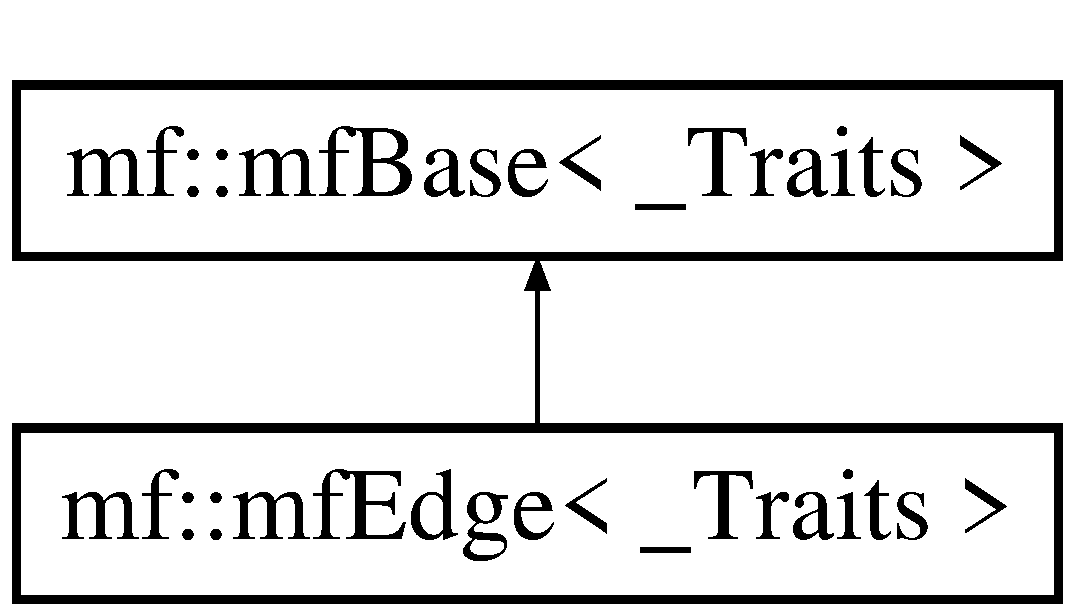
\includegraphics[height=2.000000cm]{classmf_1_1mfEdge}
\end{center}
\end{figure}
\subsection*{Public Member Functions}
\begin{DoxyCompactItemize}
\item 
\hyperlink{classmf_1_1mfEdge_a39bdf3e69fabf5d83107743e717dfca4}{mfEdge} ()
\item 
virtual \hyperlink{classmf_1_1mfEdge_a64a2c058d42cbe318eae91c9f1fff0ca}{$\sim$mfEdge} ()
\end{DoxyCompactItemize}
\subsubsection*{template$<$class \_\-Traits$>$ class mf::mfEdge$<$ \_\-Traits $>$}



\subsection{Constructor \& Destructor Documentation}
\hypertarget{classmf_1_1mfEdge_a39bdf3e69fabf5d83107743e717dfca4}{
\index{mf::mfEdge@{mf::mfEdge}!mfEdge@{mfEdge}}
\index{mfEdge@{mfEdge}!mf::mfEdge@{mf::mfEdge}}
\subsubsection[{mfEdge}]{\setlength{\rightskip}{0pt plus 5cm}template$<$class \_\-Traits $>$ {\bf mf::mfEdge}$<$ \_\-Traits $>$::{\bf mfEdge} (
\begin{DoxyParamCaption}
{}
\end{DoxyParamCaption}
)}}
\label{classmf_1_1mfEdge_a39bdf3e69fabf5d83107743e717dfca4}
Constructor

Initialize vertices and mates ids \hypertarget{classmf_1_1mfEdge_a64a2c058d42cbe318eae91c9f1fff0ca}{
\index{mf::mfEdge@{mf::mfEdge}!$\sim$mfEdge@{$\sim$mfEdge}}
\index{$\sim$mfEdge@{$\sim$mfEdge}!mf::mfEdge@{mf::mfEdge}}
\subsubsection[{$\sim$mfEdge}]{\setlength{\rightskip}{0pt plus 5cm}template$<$class \_\-Traits $>$ {\bf mf::mfEdge}$<$ \_\-Traits $>$::$\sim${\bf mfEdge} (
\begin{DoxyParamCaption}
{}
\end{DoxyParamCaption}
)\hspace{0.3cm}{\ttfamily  \mbox{[}virtual\mbox{]}}}}
\label{classmf_1_1mfEdge_a64a2c058d42cbe318eae91c9f1fff0ca}
Destructor 

The documentation for this class was generated from the following file:\begin{DoxyCompactItemize}
\item 
\hyperlink{mfEdge_8h}{mfEdge.h}\end{DoxyCompactItemize}

\hypertarget{classmf_1_1mfEdgesIterator}{
\section{mf::mfEdgesIterator$<$ \_\-Traits $>$ Class Template Reference}
\label{classmf_1_1mfEdgesIterator}\index{mf::mfEdgesIterator@{mf::mfEdgesIterator}}
}
Inheritance diagram for mf::mfEdgesIterator$<$ \_\-Traits $>$:\begin{figure}[H]
\begin{center}
\leavevmode
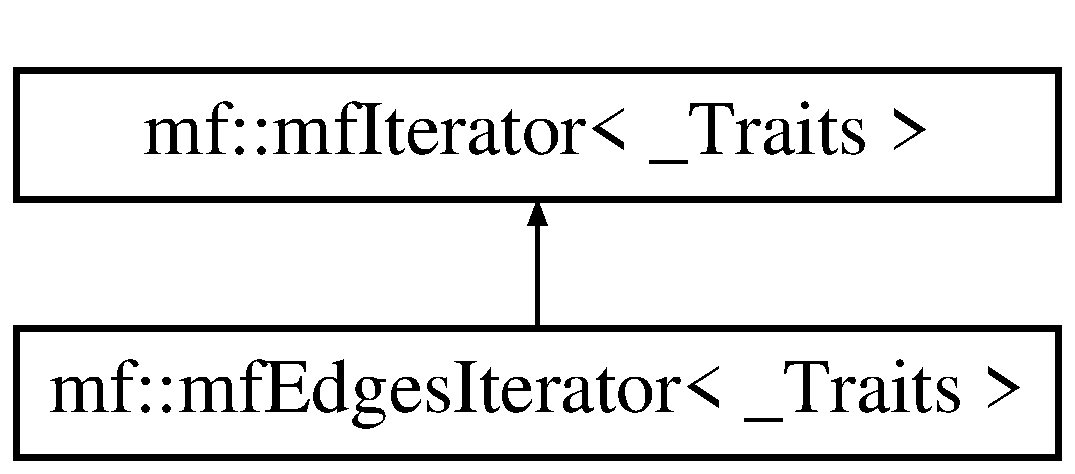
\includegraphics[height=2.000000cm]{classmf_1_1mfEdgesIterator}
\end{center}
\end{figure}
\subsection*{Public Types}
\begin{DoxyCompactItemize}
\item 
typedef \_\-Traits::sEdge \hyperlink{classmf_1_1mfEdgesIterator_afeb149d8a3c0efac598f1c13daf711b1}{sEdge}
\item 
typedef \_\-Traits::ids \hyperlink{classmf_1_1mfEdgesIterator_a6950c402f825ad11316256f59e5ae887}{ids}
\item 
typedef \_\-Traits::sMesh \hyperlink{classmf_1_1mfEdgesIterator_aef5fcd1a83c753089ba7c4e3d6f33733}{sMesh}
\end{DoxyCompactItemize}
\subsection*{Public Member Functions}
\begin{DoxyCompactItemize}
\item 
\hyperlink{classmf_1_1mfEdgesIterator_a6aa793309abbe8379814a859cdb5f913}{mfEdgesIterator} (\hyperlink{classmf_1_1mfEdgesIterator_aef5fcd1a83c753089ba7c4e3d6f33733}{sMesh} $\ast$\_\-mesh)
\item 
\hyperlink{classmf_1_1mfEdgesIterator_a479b21ac1083b71f9f6fa22424bde056}{$\sim$mfEdgesIterator} ()
\item 
\hypertarget{classmf_1_1mfEdgesIterator_af4e5ee1959a5cb92af1ccf99a88c95cf}{
bool {\bfseries initialize} (\hyperlink{classmf_1_1mfEdgesIterator_a6950c402f825ad11316256f59e5ae887}{ids} init=0)}
\label{classmf_1_1mfEdgesIterator_af4e5ee1959a5cb92af1ccf99a88c95cf}

\item 
\hypertarget{classmf_1_1mfEdgesIterator_a61de50c1c3df01e2ce79fd0f5991b666}{
bool {\bfseries finish} ()}
\label{classmf_1_1mfEdgesIterator_a61de50c1c3df01e2ce79fd0f5991b666}

\item 
\hypertarget{classmf_1_1mfEdgesIterator_ad99236b64b8c44519b8ede2077309000}{
bool {\bfseries notFinish} ()}
\label{classmf_1_1mfEdgesIterator_ad99236b64b8c44519b8ede2077309000}

\item 
\hypertarget{classmf_1_1mfEdgesIterator_ac4ddc01312209053fea6f8c520c5a462}{
bool {\bfseries operator++} ()}
\label{classmf_1_1mfEdgesIterator_ac4ddc01312209053fea6f8c520c5a462}

\item 
\hypertarget{classmf_1_1mfEdgesIterator_a9b651f17838d7555f4365690422be0ef}{
bool {\bfseries operator-\/-\/} ()}
\label{classmf_1_1mfEdgesIterator_a9b651f17838d7555f4365690422be0ef}

\item 
\hypertarget{classmf_1_1mfEdgesIterator_a15ca78291598d4c42d5484e1876da939}{
\hyperlink{classmf_1_1mfEdgesIterator_afeb149d8a3c0efac598f1c13daf711b1}{sEdge} $\ast$ {\bfseries operator-\/$>$} ()}
\label{classmf_1_1mfEdgesIterator_a15ca78291598d4c42d5484e1876da939}

\item 
\hypertarget{classmf_1_1mfEdgesIterator_a677ee3a89dd7e3425d8f2269026a2a99}{
\hyperlink{classmf_1_1mfEdgesIterator_afeb149d8a3c0efac598f1c13daf711b1}{sEdge} $\ast$ {\bfseries operator$\ast$} ()}
\label{classmf_1_1mfEdgesIterator_a677ee3a89dd7e3425d8f2269026a2a99}

\item 
\hypertarget{classmf_1_1mfEdgesIterator_a0497741f92888c2a14f4c4a01b6933a8}{
\hyperlink{classmf_1_1mfEdgesIterator_a6950c402f825ad11316256f59e5ae887}{ids} {\bfseries operator\&} ()}
\label{classmf_1_1mfEdgesIterator_a0497741f92888c2a14f4c4a01b6933a8}

\end{DoxyCompactItemize}
\subsubsection*{template$<$class \_\-Traits$>$ class mf::mfEdgesIterator$<$ \_\-Traits $>$}



\subsection{Member Typedef Documentation}
\hypertarget{classmf_1_1mfEdgesIterator_a6950c402f825ad11316256f59e5ae887}{
\index{mf::mfEdgesIterator@{mf::mfEdgesIterator}!ids@{ids}}
\index{ids@{ids}!mf::mfEdgesIterator@{mf::mfEdgesIterator}}
\subsubsection[{ids}]{\setlength{\rightskip}{0pt plus 5cm}template$<$class \_\-Traits $>$ typedef \_\-Traits::ids {\bf mf::mfEdgesIterator}$<$ \_\-Traits $>$::{\bf ids}}}
\label{classmf_1_1mfEdgesIterator_a6950c402f825ad11316256f59e5ae887}
Id typename definition \hypertarget{classmf_1_1mfEdgesIterator_afeb149d8a3c0efac598f1c13daf711b1}{
\index{mf::mfEdgesIterator@{mf::mfEdgesIterator}!sEdge@{sEdge}}
\index{sEdge@{sEdge}!mf::mfEdgesIterator@{mf::mfEdgesIterator}}
\subsubsection[{sEdge}]{\setlength{\rightskip}{0pt plus 5cm}template$<$class \_\-Traits $>$ typedef \_\-Traits::sEdge {\bf mf::mfEdgesIterator}$<$ \_\-Traits $>$::{\bf sEdge}}}
\label{classmf_1_1mfEdgesIterator_afeb149d8a3c0efac598f1c13daf711b1}
Edge typename definition \hypertarget{classmf_1_1mfEdgesIterator_aef5fcd1a83c753089ba7c4e3d6f33733}{
\index{mf::mfEdgesIterator@{mf::mfEdgesIterator}!sMesh@{sMesh}}
\index{sMesh@{sMesh}!mf::mfEdgesIterator@{mf::mfEdgesIterator}}
\subsubsection[{sMesh}]{\setlength{\rightskip}{0pt plus 5cm}template$<$class \_\-Traits $>$ typedef \_\-Traits::sMesh {\bf mf::mfEdgesIterator}$<$ \_\-Traits $>$::{\bf sMesh}}}
\label{classmf_1_1mfEdgesIterator_aef5fcd1a83c753089ba7c4e3d6f33733}
Mesh typename definition 

Reimplemented from \hyperlink{classmf_1_1mfIterator_aca31e4d7e7eca4e3b100530d8725064b}{mf::mfIterator$<$ \_\-Traits $>$}.



\subsection{Constructor \& Destructor Documentation}
\hypertarget{classmf_1_1mfEdgesIterator_a6aa793309abbe8379814a859cdb5f913}{
\index{mf::mfEdgesIterator@{mf::mfEdgesIterator}!mfEdgesIterator@{mfEdgesIterator}}
\index{mfEdgesIterator@{mfEdgesIterator}!mf::mfEdgesIterator@{mf::mfEdgesIterator}}
\subsubsection[{mfEdgesIterator}]{\setlength{\rightskip}{0pt plus 5cm}template$<$class \_\-Traits $>$ {\bf mf::mfEdgesIterator}$<$ \_\-Traits $>$::{\bf mfEdgesIterator} (
\begin{DoxyParamCaption}
\item[{{\bf sMesh} $\ast$}]{\_\-mesh}
\end{DoxyParamCaption}
)}}
\label{classmf_1_1mfEdgesIterator_a6aa793309abbe8379814a859cdb5f913}
Constructor \hypertarget{classmf_1_1mfEdgesIterator_a479b21ac1083b71f9f6fa22424bde056}{
\index{mf::mfEdgesIterator@{mf::mfEdgesIterator}!$\sim$mfEdgesIterator@{$\sim$mfEdgesIterator}}
\index{$\sim$mfEdgesIterator@{$\sim$mfEdgesIterator}!mf::mfEdgesIterator@{mf::mfEdgesIterator}}
\subsubsection[{$\sim$mfEdgesIterator}]{\setlength{\rightskip}{0pt plus 5cm}template$<$class \_\-Traits $>$ {\bf mf::mfEdgesIterator}$<$ \_\-Traits $>$::$\sim${\bf mfEdgesIterator} (
\begin{DoxyParamCaption}
{}
\end{DoxyParamCaption}
)}}
\label{classmf_1_1mfEdgesIterator_a479b21ac1083b71f9f6fa22424bde056}
Destructor 

The documentation for this class was generated from the following file:\begin{DoxyCompactItemize}
\item 
\hyperlink{mfEdgesIterator_8h}{mfEdgesIterator.h}\end{DoxyCompactItemize}

\hypertarget{classmf_1_1mfEdgeStarIterator3D}{
\section{mf::mfEdgeStarIterator3D$<$ \_\-Traits $>$ Class Template Reference}
\label{classmf_1_1mfEdgeStarIterator3D}\index{mf::mfEdgeStarIterator3D@{mf::mfEdgeStarIterator3D}}
}
Inheritance diagram for mf::mfEdgeStarIterator3D$<$ \_\-Traits $>$:\begin{figure}[H]
\begin{center}
\leavevmode
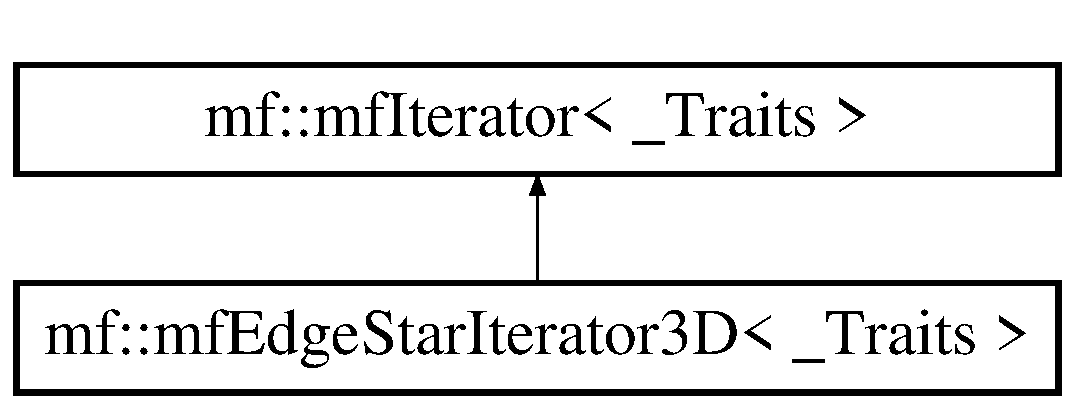
\includegraphics[height=2.000000cm]{classmf_1_1mfEdgeStarIterator3D}
\end{center}
\end{figure}
\subsection*{Public Types}
\begin{DoxyCompactItemize}
\item 
\hypertarget{classmf_1_1mfEdgeStarIterator3D_a5c76cd481f15715626ca2a2c4506f98c}{
typedef \_\-Traits::sCell {\bfseries sCell}}
\label{classmf_1_1mfEdgeStarIterator3D_a5c76cd481f15715626ca2a2c4506f98c}

\item 
\hypertarget{classmf_1_1mfEdgeStarIterator3D_ac90b77401bc37713469966adc455e26f}{
typedef \_\-Traits::sVertex {\bfseries sVertex}}
\label{classmf_1_1mfEdgeStarIterator3D_ac90b77401bc37713469966adc455e26f}

\item 
\hypertarget{classmf_1_1mfEdgeStarIterator3D_a198d164988ab98289413715bdf1c159c}{
typedef \_\-Traits::ids {\bfseries ids}}
\label{classmf_1_1mfEdgeStarIterator3D_a198d164988ab98289413715bdf1c159c}

\item 
\hypertarget{classmf_1_1mfEdgeStarIterator3D_aab9f99937505b81da093118cd53dafc0}{
typedef \hyperlink{classmf_1_1mfSing}{mfSing}$<$ \_\-Traits $>$ {\bfseries sSing}}
\label{classmf_1_1mfEdgeStarIterator3D_aab9f99937505b81da093118cd53dafc0}

\item 
typedef \_\-Traits::sMesh \hyperlink{classmf_1_1mfEdgeStarIterator3D_a875ac7316bdc779e38b0a8befde57366}{sMesh}
\end{DoxyCompactItemize}
\subsection*{Public Member Functions}
\begin{DoxyCompactItemize}
\item 
\hyperlink{classmf_1_1mfEdgeStarIterator3D_a9dc421576d690d367e42900b5ace8e86}{mfEdgeStarIterator3D} (\hyperlink{classmf_1_1mfEdgeStarIterator3D_a875ac7316bdc779e38b0a8befde57366}{sMesh} $\ast$\_\-mesh)
\item 
\hyperlink{classmf_1_1mfEdgeStarIterator3D_a51c3e5a707ab22d500f785177c60beab}{$\sim$mfEdgeStarIterator3D} ()
\item 
\hypertarget{classmf_1_1mfEdgeStarIterator3D_aca589c444d58332ee236be5b73bc30ba}{
bool {\bfseries initialize} (ids idcell, int index1, int index2)}
\label{classmf_1_1mfEdgeStarIterator3D_aca589c444d58332ee236be5b73bc30ba}

\item 
\hypertarget{classmf_1_1mfEdgeStarIterator3D_af1bce3b4e18b794cfa6ed8a202f018a5}{
bool {\bfseries finish} ()}
\label{classmf_1_1mfEdgeStarIterator3D_af1bce3b4e18b794cfa6ed8a202f018a5}

\item 
\hypertarget{classmf_1_1mfEdgeStarIterator3D_a5c6a91a3e100b9f3b7f2908496240e97}{
bool {\bfseries notFinish} ()}
\label{classmf_1_1mfEdgeStarIterator3D_a5c6a91a3e100b9f3b7f2908496240e97}

\item 
\hypertarget{classmf_1_1mfEdgeStarIterator3D_a87f4b136dd0acf703a75dbf0744f029b}{
bool {\bfseries operator++} ()}
\label{classmf_1_1mfEdgeStarIterator3D_a87f4b136dd0acf703a75dbf0744f029b}

\item 
\hypertarget{classmf_1_1mfEdgeStarIterator3D_aaa92619beac64e3a04efeaf8140a5996}{
sCell $\ast$ {\bfseries operator-\/$>$} ()}
\label{classmf_1_1mfEdgeStarIterator3D_aaa92619beac64e3a04efeaf8140a5996}

\item 
\hypertarget{classmf_1_1mfEdgeStarIterator3D_ad2f8ffb9066b075f6b11b6c62bf05911}{
sCell $\ast$ {\bfseries operator$\ast$} ()}
\label{classmf_1_1mfEdgeStarIterator3D_ad2f8ffb9066b075f6b11b6c62bf05911}

\item 
\hypertarget{classmf_1_1mfEdgeStarIterator3D_ad9a32e1ed5a6d63f07c5fe2d6dea6f8b}{
ids {\bfseries operator\&} ()}
\label{classmf_1_1mfEdgeStarIterator3D_ad9a32e1ed5a6d63f07c5fe2d6dea6f8b}

\end{DoxyCompactItemize}
\subsubsection*{template$<$class \_\-Traits$>$ class mf::mfEdgeStarIterator3D$<$ \_\-Traits $>$}



\subsection{Member Typedef Documentation}
\hypertarget{classmf_1_1mfEdgeStarIterator3D_a875ac7316bdc779e38b0a8befde57366}{
\index{mf::mfEdgeStarIterator3D@{mf::mfEdgeStarIterator3D}!sMesh@{sMesh}}
\index{sMesh@{sMesh}!mf::mfEdgeStarIterator3D@{mf::mfEdgeStarIterator3D}}
\subsubsection[{sMesh}]{\setlength{\rightskip}{0pt plus 5cm}template$<$class \_\-Traits $>$ typedef \_\-Traits::sMesh {\bf mf::mfEdgeStarIterator3D}$<$ \_\-Traits $>$::{\bf sMesh}}}
\label{classmf_1_1mfEdgeStarIterator3D_a875ac7316bdc779e38b0a8befde57366}
Mesh typename definition 

Reimplemented from \hyperlink{classmf_1_1mfIterator_aca31e4d7e7eca4e3b100530d8725064b}{mf::mfIterator$<$ \_\-Traits $>$}.



\subsection{Constructor \& Destructor Documentation}
\hypertarget{classmf_1_1mfEdgeStarIterator3D_a9dc421576d690d367e42900b5ace8e86}{
\index{mf::mfEdgeStarIterator3D@{mf::mfEdgeStarIterator3D}!mfEdgeStarIterator3D@{mfEdgeStarIterator3D}}
\index{mfEdgeStarIterator3D@{mfEdgeStarIterator3D}!mf::mfEdgeStarIterator3D@{mf::mfEdgeStarIterator3D}}
\subsubsection[{mfEdgeStarIterator3D}]{\setlength{\rightskip}{0pt plus 5cm}template$<$class \_\-Traits $>$ {\bf mf::mfEdgeStarIterator3D}$<$ \_\-Traits $>$::{\bf mfEdgeStarIterator3D} (
\begin{DoxyParamCaption}
\item[{{\bf sMesh} $\ast$}]{\_\-mesh}
\end{DoxyParamCaption}
)}}
\label{classmf_1_1mfEdgeStarIterator3D_a9dc421576d690d367e42900b5ace8e86}
Construtor \hypertarget{classmf_1_1mfEdgeStarIterator3D_a51c3e5a707ab22d500f785177c60beab}{
\index{mf::mfEdgeStarIterator3D@{mf::mfEdgeStarIterator3D}!$\sim$mfEdgeStarIterator3D@{$\sim$mfEdgeStarIterator3D}}
\index{$\sim$mfEdgeStarIterator3D@{$\sim$mfEdgeStarIterator3D}!mf::mfEdgeStarIterator3D@{mf::mfEdgeStarIterator3D}}
\subsubsection[{$\sim$mfEdgeStarIterator3D}]{\setlength{\rightskip}{0pt plus 5cm}template$<$class \_\-Traits $>$ {\bf mf::mfEdgeStarIterator3D}$<$ \_\-Traits $>$::$\sim${\bf mfEdgeStarIterator3D} (
\begin{DoxyParamCaption}
{}
\end{DoxyParamCaption}
)}}
\label{classmf_1_1mfEdgeStarIterator3D_a51c3e5a707ab22d500f785177c60beab}
Destrutor 

The documentation for this class was generated from the following file:\begin{DoxyCompactItemize}
\item 
mfEdgeStarIterator3D.h\end{DoxyCompactItemize}

\hypertarget{classmf_1_1mfEdgeStarIteratorTetra}{
\section{mf::mfEdgeStarIteratorTetra$<$ \_\-Traits $>$ Class Template Reference}
\label{classmf_1_1mfEdgeStarIteratorTetra}\index{mf::mfEdgeStarIteratorTetra@{mf::mfEdgeStarIteratorTetra}}
}
Inheritance diagram for mf::mfEdgeStarIteratorTetra$<$ \_\-Traits $>$:\begin{figure}[H]
\begin{center}
\leavevmode
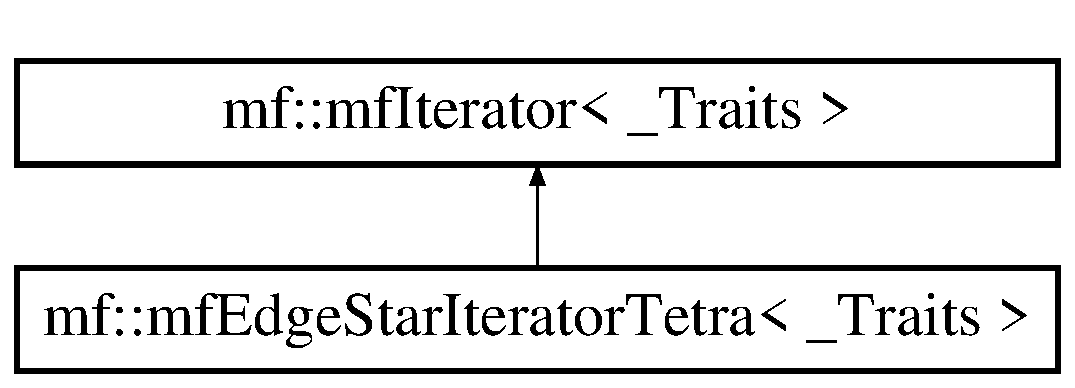
\includegraphics[height=2.000000cm]{classmf_1_1mfEdgeStarIteratorTetra}
\end{center}
\end{figure}
\subsection*{Public Types}
\begin{DoxyCompactItemize}
\item 
\hypertarget{classmf_1_1mfEdgeStarIteratorTetra_af5ea46fe004d7712f91d6059b67c6754}{
typedef \_\-Traits::sCell {\bfseries sCell}}
\label{classmf_1_1mfEdgeStarIteratorTetra_af5ea46fe004d7712f91d6059b67c6754}

\item 
\hypertarget{classmf_1_1mfEdgeStarIteratorTetra_a3ee0be7a8bd43274196ae7448bd5b3e5}{
typedef \_\-Traits::sVertex {\bfseries sVertex}}
\label{classmf_1_1mfEdgeStarIteratorTetra_a3ee0be7a8bd43274196ae7448bd5b3e5}

\item 
\hypertarget{classmf_1_1mfEdgeStarIteratorTetra_afb4c9a31307581a7bf461acdf3508e63}{
typedef \_\-Traits::ids {\bfseries ids}}
\label{classmf_1_1mfEdgeStarIteratorTetra_afb4c9a31307581a7bf461acdf3508e63}

\item 
\hypertarget{classmf_1_1mfEdgeStarIteratorTetra_a66677bff586f449a4c176a2c766a17ac}{
typedef \hyperlink{classmf_1_1mfSing}{mfSing}$<$ \_\-Traits $>$ {\bfseries sSing}}
\label{classmf_1_1mfEdgeStarIteratorTetra_a66677bff586f449a4c176a2c766a17ac}

\item 
typedef \_\-Traits::sMesh \hyperlink{classmf_1_1mfEdgeStarIteratorTetra_abbb7ca848037b976d69368943567397b}{sMesh}
\end{DoxyCompactItemize}
\subsection*{Public Member Functions}
\begin{DoxyCompactItemize}
\item 
\hyperlink{classmf_1_1mfEdgeStarIteratorTetra_a74901b681190a2e930f4ce3c0df7b144}{mfEdgeStarIteratorTetra} (\hyperlink{classmf_1_1mfEdgeStarIteratorTetra_abbb7ca848037b976d69368943567397b}{sMesh} $\ast$\_\-mesh)
\item 
\hyperlink{classmf_1_1mfEdgeStarIteratorTetra_aa5af0640ad94c07a0ac86a8465cb3acf}{$\sim$mfEdgeStarIteratorTetra} ()
\item 
\hypertarget{classmf_1_1mfEdgeStarIteratorTetra_a12d177e0318a308de5cd640c144e5e32}{
bool {\bfseries initialize} (ids idcell, int index1, int index2)}
\label{classmf_1_1mfEdgeStarIteratorTetra_a12d177e0318a308de5cd640c144e5e32}

\item 
\hypertarget{classmf_1_1mfEdgeStarIteratorTetra_a52ebfd7ebca1f186f09ae3848dbe3d67}{
bool {\bfseries finish} ()}
\label{classmf_1_1mfEdgeStarIteratorTetra_a52ebfd7ebca1f186f09ae3848dbe3d67}

\item 
\hypertarget{classmf_1_1mfEdgeStarIteratorTetra_a6d4d34a65c49bc3ddd28150ab80280f9}{
bool {\bfseries notFinish} ()}
\label{classmf_1_1mfEdgeStarIteratorTetra_a6d4d34a65c49bc3ddd28150ab80280f9}

\item 
\hypertarget{classmf_1_1mfEdgeStarIteratorTetra_a0ab22331145fa1de75871913d7715025}{
bool {\bfseries operator++} ()}
\label{classmf_1_1mfEdgeStarIteratorTetra_a0ab22331145fa1de75871913d7715025}

\item 
\hypertarget{classmf_1_1mfEdgeStarIteratorTetra_a16ba2b3bd9f7ae2f9919addf1d637e46}{
sCell $\ast$ {\bfseries operator-\/$>$} ()}
\label{classmf_1_1mfEdgeStarIteratorTetra_a16ba2b3bd9f7ae2f9919addf1d637e46}

\item 
\hypertarget{classmf_1_1mfEdgeStarIteratorTetra_ab3f769b5de3b28d2fdd1fcaca2787e43}{
sCell $\ast$ {\bfseries operator$\ast$} ()}
\label{classmf_1_1mfEdgeStarIteratorTetra_ab3f769b5de3b28d2fdd1fcaca2787e43}

\item 
\hypertarget{classmf_1_1mfEdgeStarIteratorTetra_ad8b4e222f823e1dd6f394419b5eb2b61}{
ids {\bfseries operator\&} ()}
\label{classmf_1_1mfEdgeStarIteratorTetra_ad8b4e222f823e1dd6f394419b5eb2b61}

\item 
\hypertarget{classmf_1_1mfEdgeStarIteratorTetra_a0d0415bf2ff9a6b16607db1ba2bc1788}{
int {\bfseries getV1Index} ()}
\label{classmf_1_1mfEdgeStarIteratorTetra_a0d0415bf2ff9a6b16607db1ba2bc1788}

\item 
\hypertarget{classmf_1_1mfEdgeStarIteratorTetra_ab50da99eaf2bb0d293e48a7687bad9fd}{
int {\bfseries getV2Index} ()}
\label{classmf_1_1mfEdgeStarIteratorTetra_ab50da99eaf2bb0d293e48a7687bad9fd}

\end{DoxyCompactItemize}
\subsubsection*{template$<$class \_\-Traits$>$ class mf::mfEdgeStarIteratorTetra$<$ \_\-Traits $>$}



\subsection{Member Typedef Documentation}
\hypertarget{classmf_1_1mfEdgeStarIteratorTetra_abbb7ca848037b976d69368943567397b}{
\index{mf::mfEdgeStarIteratorTetra@{mf::mfEdgeStarIteratorTetra}!sMesh@{sMesh}}
\index{sMesh@{sMesh}!mf::mfEdgeStarIteratorTetra@{mf::mfEdgeStarIteratorTetra}}
\subsubsection[{sMesh}]{\setlength{\rightskip}{0pt plus 5cm}template$<$class \_\-Traits $>$ typedef \_\-Traits::sMesh {\bf mf::mfEdgeStarIteratorTetra}$<$ \_\-Traits $>$::{\bf sMesh}}}
\label{classmf_1_1mfEdgeStarIteratorTetra_abbb7ca848037b976d69368943567397b}
Mesh typename definition 

Reimplemented from \hyperlink{classmf_1_1mfIterator_aca31e4d7e7eca4e3b100530d8725064b}{mf::mfIterator$<$ \_\-Traits $>$}.



\subsection{Constructor \& Destructor Documentation}
\hypertarget{classmf_1_1mfEdgeStarIteratorTetra_a74901b681190a2e930f4ce3c0df7b144}{
\index{mf::mfEdgeStarIteratorTetra@{mf::mfEdgeStarIteratorTetra}!mfEdgeStarIteratorTetra@{mfEdgeStarIteratorTetra}}
\index{mfEdgeStarIteratorTetra@{mfEdgeStarIteratorTetra}!mf::mfEdgeStarIteratorTetra@{mf::mfEdgeStarIteratorTetra}}
\subsubsection[{mfEdgeStarIteratorTetra}]{\setlength{\rightskip}{0pt plus 5cm}template$<$class \_\-Traits $>$ {\bf mf::mfEdgeStarIteratorTetra}$<$ \_\-Traits $>$::{\bf mfEdgeStarIteratorTetra} (
\begin{DoxyParamCaption}
\item[{{\bf sMesh} $\ast$}]{\_\-mesh}
\end{DoxyParamCaption}
)}}
\label{classmf_1_1mfEdgeStarIteratorTetra_a74901b681190a2e930f4ce3c0df7b144}
Construtor \hypertarget{classmf_1_1mfEdgeStarIteratorTetra_aa5af0640ad94c07a0ac86a8465cb3acf}{
\index{mf::mfEdgeStarIteratorTetra@{mf::mfEdgeStarIteratorTetra}!$\sim$mfEdgeStarIteratorTetra@{$\sim$mfEdgeStarIteratorTetra}}
\index{$\sim$mfEdgeStarIteratorTetra@{$\sim$mfEdgeStarIteratorTetra}!mf::mfEdgeStarIteratorTetra@{mf::mfEdgeStarIteratorTetra}}
\subsubsection[{$\sim$mfEdgeStarIteratorTetra}]{\setlength{\rightskip}{0pt plus 5cm}template$<$class \_\-Traits $>$ {\bf mf::mfEdgeStarIteratorTetra}$<$ \_\-Traits $>$::$\sim${\bf mfEdgeStarIteratorTetra} (
\begin{DoxyParamCaption}
{}
\end{DoxyParamCaption}
)}}
\label{classmf_1_1mfEdgeStarIteratorTetra_aa5af0640ad94c07a0ac86a8465cb3acf}
Destrutor 

The documentation for this class was generated from the following file:\begin{DoxyCompactItemize}
\item 
mfEdgeStarIteratorTetra.h\end{DoxyCompactItemize}

\hypertarget{classmf_1_1mfFace}{
\section{mf::mfFace$<$ \_\-Traits $>$ Class Template Reference}
\label{classmf_1_1mfFace}\index{mf::mfFace@{mf::mfFace}}
}
Inheritance diagram for mf::mfFace$<$ \_\-Traits $>$:\begin{figure}[H]
\begin{center}
\leavevmode
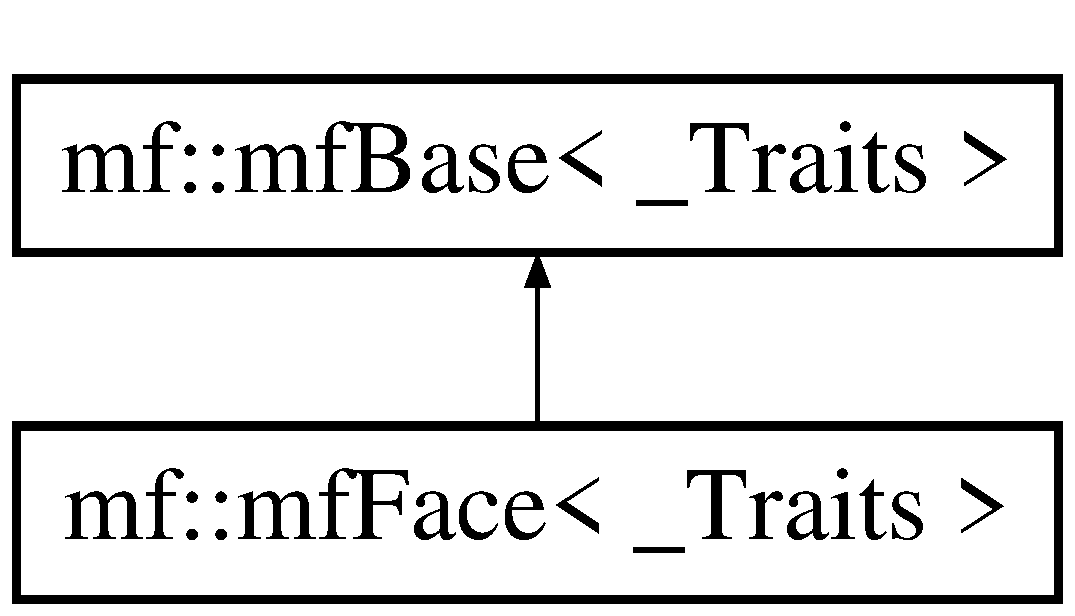
\includegraphics[height=2.000000cm]{classmf_1_1mfFace}
\end{center}
\end{figure}
\subsection*{Public Member Functions}
\begin{DoxyCompactItemize}
\item 
\hyperlink{classmf_1_1mfFace_a2fccb539e46b2a176fa9e04977571374}{mfFace} ()
\item 
virtual \hyperlink{classmf_1_1mfFace_a9cd731f61c4587b9087634236eb9a37f}{$\sim$mfFace} ()
\end{DoxyCompactItemize}
\subsubsection*{template$<$class \_\-Traits$>$ class mf::mfFace$<$ \_\-Traits $>$}



\subsection{Constructor \& Destructor Documentation}
\hypertarget{classmf_1_1mfFace_a2fccb539e46b2a176fa9e04977571374}{
\index{mf::mfFace@{mf::mfFace}!mfFace@{mfFace}}
\index{mfFace@{mfFace}!mf::mfFace@{mf::mfFace}}
\subsubsection[{mfFace}]{\setlength{\rightskip}{0pt plus 5cm}template$<$class \_\-Traits $>$ {\bf mf::mfFace}$<$ \_\-Traits $>$::{\bf mfFace} (
\begin{DoxyParamCaption}
{}
\end{DoxyParamCaption}
)}}
\label{classmf_1_1mfFace_a2fccb539e46b2a176fa9e04977571374}
Constructor

Initialize vertices and mates ids \hypertarget{classmf_1_1mfFace_a9cd731f61c4587b9087634236eb9a37f}{
\index{mf::mfFace@{mf::mfFace}!$\sim$mfFace@{$\sim$mfFace}}
\index{$\sim$mfFace@{$\sim$mfFace}!mf::mfFace@{mf::mfFace}}
\subsubsection[{$\sim$mfFace}]{\setlength{\rightskip}{0pt plus 5cm}template$<$class \_\-Traits $>$ {\bf mf::mfFace}$<$ \_\-Traits $>$::$\sim${\bf mfFace} (
\begin{DoxyParamCaption}
{}
\end{DoxyParamCaption}
)\hspace{0.3cm}{\ttfamily  \mbox{[}virtual\mbox{]}}}}
\label{classmf_1_1mfFace_a9cd731f61c4587b9087634236eb9a37f}
Destructor 

The documentation for this class was generated from the following file:\begin{DoxyCompactItemize}
\item 
\hyperlink{mfFace_8h}{mfFace.h}\end{DoxyCompactItemize}

\hypertarget{classmf_1_1mfGeometric}{
\section{mf::mfGeometric$<$ \_\-Traits $>$ Class Template Reference}
\label{classmf_1_1mfGeometric}\index{mf::mfGeometric@{mf::mfGeometric}}
}
\subsection*{Public Types}
\begin{DoxyCompactItemize}
\item 
typedef \_\-Traits::space \hyperlink{classmf_1_1mfGeometric_a03504b73c011add763229b5bae6e137c}{space}
\item 
typedef \_\-Traits::ids \hyperlink{classmf_1_1mfGeometric_a15bbb64e3b03482d20c82fa2d4b68e56}{ids}
\item 
typedef \_\-Traits::sVertex \hyperlink{classmf_1_1mfGeometric_a6195106d9ab499c9c59532d804d6eacf}{sVertex}
\item 
typedef \_\-Traits::sCell \hyperlink{classmf_1_1mfGeometric_a59004ce8cd63aa64c7a6ce66eb6f0080}{sCell}
\item 
typedef \hyperlink{classmf_1_1mfSing}{mfSing}$<$ \_\-Traits $>$ \hyperlink{classmf_1_1mfGeometric_a1fe080907992c40828062aac0717fc13}{sSing}
\item 
typedef \_\-Traits::sMesh \hyperlink{classmf_1_1mfGeometric_a36b13b57c06fda7c04e3202ad1dae4d2}{sMesh}
\end{DoxyCompactItemize}
\subsection*{Public Member Functions}
\begin{DoxyCompactItemize}
\item 
\hyperlink{classmf_1_1mfGeometric_a80e5d1b4e9e47785128e576554fc0323}{mfGeometric} (\hyperlink{classmf_1_1mfGeometric_a36b13b57c06fda7c04e3202ad1dae4d2}{sMesh} $\ast$\_\-mesh=NULL, double \_\-erro=MF\_\-ERRO)
\item 
\hyperlink{classmf_1_1mfGeometric_a7ec6a2f8930e7d7020acb33e1d895f76}{$\sim$mfGeometric} ()
\item 
void \hyperlink{classmf_1_1mfGeometric_a2f47c5feb979cf56cd502e621dbab584}{setMesh} (\hyperlink{classmf_1_1mfGeometric_a36b13b57c06fda7c04e3202ad1dae4d2}{sMesh} $\ast$\_\-mesh)
\item 
\hypertarget{classmf_1_1mfGeometric_a4dccc2510e7436b910a84dfcb87182ce}{
int {\bfseries inLeft} (\hyperlink{classmf_1_1mfGeometric_a6195106d9ab499c9c59532d804d6eacf}{sVertex} $\ast$p0, \hyperlink{classmf_1_1mfGeometric_a6195106d9ab499c9c59532d804d6eacf}{sVertex} $\ast$p1, \hyperlink{classmf_1_1mfGeometric_a6195106d9ab499c9c59532d804d6eacf}{sVertex} $\ast$p2 MF\_\-DMUTEXVD)}
\label{classmf_1_1mfGeometric_a4dccc2510e7436b910a84dfcb87182ce}

\item 
\hypertarget{classmf_1_1mfGeometric_a3846317c8b191d4ce4b836cd7c7ceda9}{
int {\bfseries inLeft} (\hyperlink{classmf_1_1mfGeometric_a6195106d9ab499c9c59532d804d6eacf}{sVertex} $\ast$p0, \hyperlink{classmf_1_1mfGeometric_a6195106d9ab499c9c59532d804d6eacf}{sVertex} $\ast$p1, \hyperlink{classmf_1_1mfGeometric_a03504b73c011add763229b5bae6e137c}{space} coord0, \hyperlink{classmf_1_1mfGeometric_a03504b73c011add763229b5bae6e137c}{space} coord1 MF\_\-DMUTEXVD)}
\label{classmf_1_1mfGeometric_a3846317c8b191d4ce4b836cd7c7ceda9}

\item 
\hypertarget{classmf_1_1mfGeometric_a6a70182d43e4e1c6a22202db7f26f301}{
int {\bfseries inLeft} (\hyperlink{classmf_1_1mfGeometric_a15bbb64e3b03482d20c82fa2d4b68e56}{ids} p0, \hyperlink{classmf_1_1mfGeometric_a15bbb64e3b03482d20c82fa2d4b68e56}{ids} p1, \hyperlink{classmf_1_1mfGeometric_a15bbb64e3b03482d20c82fa2d4b68e56}{ids} p2 MF\_\-DMUTEXVD)}
\label{classmf_1_1mfGeometric_a6a70182d43e4e1c6a22202db7f26f301}

\item 
\hypertarget{classmf_1_1mfGeometric_a810decfaa701bde3a90a1899ad23f291}{
int {\bfseries inLeft} (\hyperlink{classmf_1_1mfGeometric_a15bbb64e3b03482d20c82fa2d4b68e56}{ids} p0, \hyperlink{classmf_1_1mfGeometric_a15bbb64e3b03482d20c82fa2d4b68e56}{ids} p1, \hyperlink{classmf_1_1mfGeometric_a03504b73c011add763229b5bae6e137c}{space} coord0, \hyperlink{classmf_1_1mfGeometric_a03504b73c011add763229b5bae6e137c}{space} coord1 MF\_\-DMUTEXVD)}
\label{classmf_1_1mfGeometric_a810decfaa701bde3a90a1899ad23f291}

\item 
\hypertarget{classmf_1_1mfGeometric_ac611c839c2490a8955ab352143e79d0c}{
\hyperlink{classmf_1_1mfGeometric_a03504b73c011add763229b5bae6e137c}{space} {\bfseries dist} (\hyperlink{classmf_1_1mfGeometric_a6195106d9ab499c9c59532d804d6eacf}{sVertex} $\ast$p0, \hyperlink{classmf_1_1mfGeometric_a6195106d9ab499c9c59532d804d6eacf}{sVertex} $\ast$p1 MF\_\-DMUTEXVD)}
\label{classmf_1_1mfGeometric_ac611c839c2490a8955ab352143e79d0c}

\item 
\hypertarget{classmf_1_1mfGeometric_ac060aaa2231f36b1acc0b5b922f5fdca}{
\hyperlink{classmf_1_1mfGeometric_a03504b73c011add763229b5bae6e137c}{space} {\bfseries dist} (\hyperlink{classmf_1_1mfGeometric_a03504b73c011add763229b5bae6e137c}{space} $\ast$p0, \hyperlink{classmf_1_1mfGeometric_a03504b73c011add763229b5bae6e137c}{space} $\ast$p1 MF\_\-DMUTEXV)}
\label{classmf_1_1mfGeometric_ac060aaa2231f36b1acc0b5b922f5fdca}

\item 
\hypertarget{classmf_1_1mfGeometric_af561b6aba2db79debd70df798bbc0e2d}{
int {\bfseries inCircle} (\hyperlink{classmf_1_1mfGeometric_a59004ce8cd63aa64c7a6ce66eb6f0080}{sCell} $\ast$c, \hyperlink{classmf_1_1mfGeometric_a6195106d9ab499c9c59532d804d6eacf}{sVertex} $\ast$p MF\_\-DMUTEXVD)}
\label{classmf_1_1mfGeometric_af561b6aba2db79debd70df798bbc0e2d}

\item 
\hypertarget{classmf_1_1mfGeometric_a62bf1cec8b78f7fad262f37b0bc72b87}{
int {\bfseries inCircle} (\hyperlink{classmf_1_1mfGeometric_a6195106d9ab499c9c59532d804d6eacf}{sVertex} $\ast$p1, \hyperlink{classmf_1_1mfGeometric_a6195106d9ab499c9c59532d804d6eacf}{sVertex} $\ast$p2, \hyperlink{classmf_1_1mfGeometric_a6195106d9ab499c9c59532d804d6eacf}{sVertex} $\ast$p3, \hyperlink{classmf_1_1mfGeometric_a6195106d9ab499c9c59532d804d6eacf}{sVertex} $\ast$p)}
\label{classmf_1_1mfGeometric_a62bf1cec8b78f7fad262f37b0bc72b87}

\item 
\hypertarget{classmf_1_1mfGeometric_a0e742fb2eac268f22a20064ced46b3d9}{
int {\bfseries pointInTetrahedron} (\hyperlink{classmf_1_1mfGeometric_a59004ce8cd63aa64c7a6ce66eb6f0080}{sCell} $\ast$c, \hyperlink{classmf_1_1mfGeometric_a6195106d9ab499c9c59532d804d6eacf}{sVertex} $\ast$p MF\_\-DMUTEXVD)}
\label{classmf_1_1mfGeometric_a0e742fb2eac268f22a20064ced46b3d9}

\item 
\hypertarget{classmf_1_1mfGeometric_aebf486718bff6b59fbefd0c0f289d9a3}{
int {\bfseries pointInTetrahedron} (\hyperlink{classmf_1_1mfGeometric_a6195106d9ab499c9c59532d804d6eacf}{sVertex} $\ast$p0, \hyperlink{classmf_1_1mfGeometric_a6195106d9ab499c9c59532d804d6eacf}{sVertex} $\ast$p1, \hyperlink{classmf_1_1mfGeometric_a6195106d9ab499c9c59532d804d6eacf}{sVertex} $\ast$p2, \hyperlink{classmf_1_1mfGeometric_a6195106d9ab499c9c59532d804d6eacf}{sVertex} $\ast$p3, \hyperlink{classmf_1_1mfGeometric_a6195106d9ab499c9c59532d804d6eacf}{sVertex} $\ast$p)}
\label{classmf_1_1mfGeometric_aebf486718bff6b59fbefd0c0f289d9a3}

\item 
\hypertarget{classmf_1_1mfGeometric_afa51150f78ee77d7239f241423d70eb0}{
bool {\bfseries inDiametralCircle} (\hyperlink{classmf_1_1mfGeometric_a6195106d9ab499c9c59532d804d6eacf}{sVertex} $\ast$v1, \hyperlink{classmf_1_1mfGeometric_a6195106d9ab499c9c59532d804d6eacf}{sVertex} $\ast$v2, \hyperlink{classmf_1_1mfGeometric_a6195106d9ab499c9c59532d804d6eacf}{sVertex} $\ast$v MF\_\-DMUTEXVD)}
\label{classmf_1_1mfGeometric_afa51150f78ee77d7239f241423d70eb0}

\item 
\hypertarget{classmf_1_1mfGeometric_ac79eaaee7be7c50d3701e08ce390c5e6}{
bool {\bfseries sameVertices} (\hyperlink{classmf_1_1mfGeometric_a6195106d9ab499c9c59532d804d6eacf}{sVertex} $\ast$v1, \hyperlink{classmf_1_1mfGeometric_a6195106d9ab499c9c59532d804d6eacf}{sVertex} $\ast$v2 MF\_\-DMUTEXVD)}
\label{classmf_1_1mfGeometric_ac79eaaee7be7c50d3701e08ce390c5e6}

\item 
\hypertarget{classmf_1_1mfGeometric_abc9102fdd97b35038785fa7707f7a4e4}{
int {\bfseries orientation2D} (\hyperlink{classmf_1_1mfGeometric_a15bbb64e3b03482d20c82fa2d4b68e56}{ids} $\ast$idvertices, \hyperlink{classmf_1_1mfGeometric_a6195106d9ab499c9c59532d804d6eacf}{sVertex} $\ast$$\ast$vertices MF\_\-DMUTEXVD)}
\label{classmf_1_1mfGeometric_abc9102fdd97b35038785fa7707f7a4e4}

\item 
\hypertarget{classmf_1_1mfGeometric_a6c9a86f83ad65021bdfd0d37ae2f5729}{
int {\bfseries orientation3D} (\hyperlink{classmf_1_1mfGeometric_a15bbb64e3b03482d20c82fa2d4b68e56}{ids} $\ast$idvertices, \hyperlink{classmf_1_1mfGeometric_a6195106d9ab499c9c59532d804d6eacf}{sVertex} $\ast$$\ast$vertices MF\_\-DMUTEXVD)}
\label{classmf_1_1mfGeometric_a6c9a86f83ad65021bdfd0d37ae2f5729}

\item 
\hypertarget{classmf_1_1mfGeometric_acb56c872c52b48528a0022d682332ef8}{
bool {\bfseries isBadCell} (\hyperlink{classmf_1_1mfGeometric_a59004ce8cd63aa64c7a6ce66eb6f0080}{sCell} $\ast$c, \hyperlink{classmf_1_1mfGeometric_a03504b73c011add763229b5bae6e137c}{space} beta MF\_\-DMUTEXVD)}
\label{classmf_1_1mfGeometric_acb56c872c52b48528a0022d682332ef8}

\item 
\hypertarget{classmf_1_1mfGeometric_a59a4f986931e55bfb576f2403fe6f81f}{
void {\bfseries getCircuncircle} (\hyperlink{classmf_1_1mfGeometric_a59004ce8cd63aa64c7a6ce66eb6f0080}{sCell} $\ast$c, \hyperlink{classmf_1_1mfGeometric_a03504b73c011add763229b5bae6e137c}{space} $\ast$coords MF\_\-DMUTEXVD)}
\label{classmf_1_1mfGeometric_a59a4f986931e55bfb576f2403fe6f81f}

\item 
\hypertarget{classmf_1_1mfGeometric_a900f817d781ab290d1d36bbac3f1128e}{
void {\bfseries getCircuncircle} (\hyperlink{classmf_1_1mfGeometric_a03504b73c011add763229b5bae6e137c}{space} $\ast$c0, \hyperlink{classmf_1_1mfGeometric_a03504b73c011add763229b5bae6e137c}{space} $\ast$c1, \hyperlink{classmf_1_1mfGeometric_a03504b73c011add763229b5bae6e137c}{space} $\ast$c2, \hyperlink{classmf_1_1mfGeometric_a03504b73c011add763229b5bae6e137c}{space} $\ast$coords MF\_\-DMUTEXV)}
\label{classmf_1_1mfGeometric_a900f817d781ab290d1d36bbac3f1128e}

\item 
\hypertarget{classmf_1_1mfGeometric_a301d6aee603c4856ce04ed055e0222d2}{
\hyperlink{classmf_1_1mfGeometric_a03504b73c011add763229b5bae6e137c}{space} {\bfseries det3} (\hyperlink{classmf_1_1mfGeometric_a03504b73c011add763229b5bae6e137c}{space} matrix\mbox{[}3\mbox{]}\mbox{[}3\mbox{]})}
\label{classmf_1_1mfGeometric_a301d6aee603c4856ce04ed055e0222d2}

\item 
\hypertarget{classmf_1_1mfGeometric_a1869b44640a65992f9f8fcea55c67dc6}{
\hyperlink{classmf_1_1mfGeometric_a03504b73c011add763229b5bae6e137c}{space} {\bfseries det} (\hyperlink{classmf_1_1mfGeometric_a03504b73c011add763229b5bae6e137c}{space} matrix\mbox{[}4\mbox{]}\mbox{[}4\mbox{]})}
\label{classmf_1_1mfGeometric_a1869b44640a65992f9f8fcea55c67dc6}

\item 
\hypertarget{classmf_1_1mfGeometric_a19cd12998d70e99775706fe92ed15a24}{
\hyperlink{classmf_1_1mfGeometric_a03504b73c011add763229b5bae6e137c}{space} {\bfseries dot} (\hyperlink{classmf_1_1mfGeometric_a15bbb64e3b03482d20c82fa2d4b68e56}{ids} p1, \hyperlink{classmf_1_1mfGeometric_a15bbb64e3b03482d20c82fa2d4b68e56}{ids} p2, \hyperlink{classmf_1_1mfGeometric_a03504b73c011add763229b5bae6e137c}{space} $\ast$coords MF\_\-DMUTEXVD)}
\label{classmf_1_1mfGeometric_a19cd12998d70e99775706fe92ed15a24}

\item 
\hypertarget{classmf_1_1mfGeometric_af982cb9dc178c6d855596e6dbf527159}{
\hyperlink{classmf_1_1mfGeometric_a03504b73c011add763229b5bae6e137c}{space} {\bfseries vecAngle} (\hyperlink{classmf_1_1mfGeometric_a15bbb64e3b03482d20c82fa2d4b68e56}{ids} p1, \hyperlink{classmf_1_1mfGeometric_a15bbb64e3b03482d20c82fa2d4b68e56}{ids} p\_\-ang, \hyperlink{classmf_1_1mfGeometric_a15bbb64e3b03482d20c82fa2d4b68e56}{ids} p2)}
\label{classmf_1_1mfGeometric_af982cb9dc178c6d855596e6dbf527159}

\item 
\hypertarget{classmf_1_1mfGeometric_acff6f48ecc51f3f6e90d605aced8a910}{
\hyperlink{classmf_1_1mfGeometric_a03504b73c011add763229b5bae6e137c}{space} {\bfseries norm2d} (\hyperlink{classmf_1_1mfGeometric_a03504b73c011add763229b5bae6e137c}{space} $\ast$coords)}
\label{classmf_1_1mfGeometric_acff6f48ecc51f3f6e90d605aced8a910}

\item 
\hypertarget{classmf_1_1mfGeometric_adff84d9c427b07a219362b04b67107db}{
\hyperlink{classmf_1_1mfGeometric_a03504b73c011add763229b5bae6e137c}{space} {\bfseries areaTriangle} (\hyperlink{classmf_1_1mfGeometric_a03504b73c011add763229b5bae6e137c}{space} $\ast$x, \hyperlink{classmf_1_1mfGeometric_a03504b73c011add763229b5bae6e137c}{space} $\ast$y, \hyperlink{classmf_1_1mfGeometric_a03504b73c011add763229b5bae6e137c}{space} $\ast$z)}
\label{classmf_1_1mfGeometric_adff84d9c427b07a219362b04b67107db}

\item 
\hypertarget{classmf_1_1mfGeometric_a92ed4ac065c390b47b22d25ddda1b711}{
bool {\bfseries isDelaunay} (\hyperlink{classmf_1_1mfGeometric_a15bbb64e3b03482d20c82fa2d4b68e56}{ids} idcell)}
\label{classmf_1_1mfGeometric_a92ed4ac065c390b47b22d25ddda1b711}

\item 
\hypertarget{classmf_1_1mfGeometric_a4d01a8e886bbf539745a087f0d734728}{
\hyperlink{classmf_1_1mfGeometric_a03504b73c011add763229b5bae6e137c}{space} {\bfseries areaTriangle} (\hyperlink{classmf_1_1mfGeometric_a59004ce8cd63aa64c7a6ce66eb6f0080}{sCell} $\ast$c)}
\label{classmf_1_1mfGeometric_a4d01a8e886bbf539745a087f0d734728}

\item 
\hypertarget{classmf_1_1mfGeometric_ae9108b2936f06bfe4e2c690e2690d3ce}{
void {\bfseries flip2D} (\hyperlink{classmf_1_1mfGeometric_a15bbb64e3b03482d20c82fa2d4b68e56}{ids} c1, \hyperlink{classmf_1_1mfGeometric_a15bbb64e3b03482d20c82fa2d4b68e56}{ids} c2 MF\_\-DMUTEXVD)}
\label{classmf_1_1mfGeometric_ae9108b2936f06bfe4e2c690e2690d3ce}

\end{DoxyCompactItemize}
\subsection*{Protected Attributes}
\begin{DoxyCompactItemize}
\item 
double \hyperlink{classmf_1_1mfGeometric_ad01313f303b880a186b941bc29f6c091}{erro}
\item 
int \hyperlink{classmf_1_1mfGeometric_a469d99476c9796b06b2c1392bc5cfcaa}{temp}
\item 
\hyperlink{classmf_1_1mfGeometric_a36b13b57c06fda7c04e3202ad1dae4d2}{sMesh} $\ast$ \hyperlink{classmf_1_1mfGeometric_a32908e210e7cca4625608a14e71403d3}{mesh}
\end{DoxyCompactItemize}
\subsubsection*{template$<$class \_\-Traits$>$ class mf::mfGeometric$<$ \_\-Traits $>$}



\subsection{Member Typedef Documentation}
\hypertarget{classmf_1_1mfGeometric_a15bbb64e3b03482d20c82fa2d4b68e56}{
\index{mf::mfGeometric@{mf::mfGeometric}!ids@{ids}}
\index{ids@{ids}!mf::mfGeometric@{mf::mfGeometric}}
\subsubsection[{ids}]{\setlength{\rightskip}{0pt plus 5cm}template$<$class \_\-Traits $>$ typedef \_\-Traits::ids {\bf mf::mfGeometric}$<$ \_\-Traits $>$::{\bf ids}}}
\label{classmf_1_1mfGeometric_a15bbb64e3b03482d20c82fa2d4b68e56}
Id typename definition \hypertarget{classmf_1_1mfGeometric_a59004ce8cd63aa64c7a6ce66eb6f0080}{
\index{mf::mfGeometric@{mf::mfGeometric}!sCell@{sCell}}
\index{sCell@{sCell}!mf::mfGeometric@{mf::mfGeometric}}
\subsubsection[{sCell}]{\setlength{\rightskip}{0pt plus 5cm}template$<$class \_\-Traits $>$ typedef \_\-Traits::sCell {\bf mf::mfGeometric}$<$ \_\-Traits $>$::{\bf sCell}}}
\label{classmf_1_1mfGeometric_a59004ce8cd63aa64c7a6ce66eb6f0080}
Cell typename definition \hypertarget{classmf_1_1mfGeometric_a36b13b57c06fda7c04e3202ad1dae4d2}{
\index{mf::mfGeometric@{mf::mfGeometric}!sMesh@{sMesh}}
\index{sMesh@{sMesh}!mf::mfGeometric@{mf::mfGeometric}}
\subsubsection[{sMesh}]{\setlength{\rightskip}{0pt plus 5cm}template$<$class \_\-Traits $>$ typedef \_\-Traits::sMesh {\bf mf::mfGeometric}$<$ \_\-Traits $>$::{\bf sMesh}}}
\label{classmf_1_1mfGeometric_a36b13b57c06fda7c04e3202ad1dae4d2}
Mesh typename definition \hypertarget{classmf_1_1mfGeometric_a03504b73c011add763229b5bae6e137c}{
\index{mf::mfGeometric@{mf::mfGeometric}!space@{space}}
\index{space@{space}!mf::mfGeometric@{mf::mfGeometric}}
\subsubsection[{space}]{\setlength{\rightskip}{0pt plus 5cm}template$<$class \_\-Traits $>$ typedef \_\-Traits::space {\bf mf::mfGeometric}$<$ \_\-Traits $>$::{\bf space}}}
\label{classmf_1_1mfGeometric_a03504b73c011add763229b5bae6e137c}
Space typename definition \hypertarget{classmf_1_1mfGeometric_a1fe080907992c40828062aac0717fc13}{
\index{mf::mfGeometric@{mf::mfGeometric}!sSing@{sSing}}
\index{sSing@{sSing}!mf::mfGeometric@{mf::mfGeometric}}
\subsubsection[{sSing}]{\setlength{\rightskip}{0pt plus 5cm}template$<$class \_\-Traits $>$ typedef {\bf mfSing}$<$\_\-Traits$>$ {\bf mf::mfGeometric}$<$ \_\-Traits $>$::{\bf sSing}}}
\label{classmf_1_1mfGeometric_a1fe080907992c40828062aac0717fc13}
Singular typename definition \hypertarget{classmf_1_1mfGeometric_a6195106d9ab499c9c59532d804d6eacf}{
\index{mf::mfGeometric@{mf::mfGeometric}!sVertex@{sVertex}}
\index{sVertex@{sVertex}!mf::mfGeometric@{mf::mfGeometric}}
\subsubsection[{sVertex}]{\setlength{\rightskip}{0pt plus 5cm}template$<$class \_\-Traits $>$ typedef \_\-Traits::sVertex {\bf mf::mfGeometric}$<$ \_\-Traits $>$::{\bf sVertex}}}
\label{classmf_1_1mfGeometric_a6195106d9ab499c9c59532d804d6eacf}
Vertex typename definition 

\subsection{Constructor \& Destructor Documentation}
\hypertarget{classmf_1_1mfGeometric_a80e5d1b4e9e47785128e576554fc0323}{
\index{mf::mfGeometric@{mf::mfGeometric}!mfGeometric@{mfGeometric}}
\index{mfGeometric@{mfGeometric}!mf::mfGeometric@{mf::mfGeometric}}
\subsubsection[{mfGeometric}]{\setlength{\rightskip}{0pt plus 5cm}template$<$class \_\-Traits $>$ {\bf mf::mfGeometric}$<$ \_\-Traits $>$::{\bf mfGeometric} (
\begin{DoxyParamCaption}
\item[{{\bf sMesh} $\ast$}]{\_\-mesh = {\ttfamily NULL}, }
\item[{double}]{\_\-erro = {\ttfamily MF\_\-ERRO}}
\end{DoxyParamCaption}
)}}
\label{classmf_1_1mfGeometric_a80e5d1b4e9e47785128e576554fc0323}
Constructor


\begin{DoxyParams}{Parameters}
{\em \_\-mesh,:} & the mesh address that this class will manipulate \\
\hline
\end{DoxyParams}
\hypertarget{classmf_1_1mfGeometric_a7ec6a2f8930e7d7020acb33e1d895f76}{
\index{mf::mfGeometric@{mf::mfGeometric}!$\sim$mfGeometric@{$\sim$mfGeometric}}
\index{$\sim$mfGeometric@{$\sim$mfGeometric}!mf::mfGeometric@{mf::mfGeometric}}
\subsubsection[{$\sim$mfGeometric}]{\setlength{\rightskip}{0pt plus 5cm}template$<$class \_\-Traits $>$ {\bf mf::mfGeometric}$<$ \_\-Traits $>$::$\sim${\bf mfGeometric} (
\begin{DoxyParamCaption}
{}
\end{DoxyParamCaption}
)}}
\label{classmf_1_1mfGeometric_a7ec6a2f8930e7d7020acb33e1d895f76}
Destructor 

\subsection{Member Function Documentation}
\hypertarget{classmf_1_1mfGeometric_a2f47c5feb979cf56cd502e621dbab584}{
\index{mf::mfGeometric@{mf::mfGeometric}!setMesh@{setMesh}}
\index{setMesh@{setMesh}!mf::mfGeometric@{mf::mfGeometric}}
\subsubsection[{setMesh}]{\setlength{\rightskip}{0pt plus 5cm}template$<$class \_\-Traits $>$ void {\bf mf::mfGeometric}$<$ \_\-Traits $>$::setMesh (
\begin{DoxyParamCaption}
\item[{{\bf sMesh} $\ast$}]{\_\-mesh}
\end{DoxyParamCaption}
)}}
\label{classmf_1_1mfGeometric_a2f47c5feb979cf56cd502e621dbab584}
Set the mesh instance to which this class will manipulate.


\begin{DoxyParams}{Parameters}
{\em \_\-mesh,:} & the mesh address that this class will manipulate \\
\hline
\end{DoxyParams}


\subsection{Member Data Documentation}
\hypertarget{classmf_1_1mfGeometric_ad01313f303b880a186b941bc29f6c091}{
\index{mf::mfGeometric@{mf::mfGeometric}!erro@{erro}}
\index{erro@{erro}!mf::mfGeometric@{mf::mfGeometric}}
\subsubsection[{erro}]{\setlength{\rightskip}{0pt plus 5cm}template$<$class \_\-Traits $>$ double {\bf mf::mfGeometric}$<$ \_\-Traits $>$::{\bf erro}\hspace{0.3cm}{\ttfamily  \mbox{[}protected\mbox{]}}}}
\label{classmf_1_1mfGeometric_ad01313f303b880a186b941bc29f6c091}
Error value limit \hypertarget{classmf_1_1mfGeometric_a32908e210e7cca4625608a14e71403d3}{
\index{mf::mfGeometric@{mf::mfGeometric}!mesh@{mesh}}
\index{mesh@{mesh}!mf::mfGeometric@{mf::mfGeometric}}
\subsubsection[{mesh}]{\setlength{\rightskip}{0pt plus 5cm}template$<$class \_\-Traits $>$ {\bf sMesh}$\ast$ {\bf mf::mfGeometric}$<$ \_\-Traits $>$::{\bf mesh}\hspace{0.3cm}{\ttfamily  \mbox{[}protected\mbox{]}}}}
\label{classmf_1_1mfGeometric_a32908e210e7cca4625608a14e71403d3}
The mesh that this class will manipulate \hypertarget{classmf_1_1mfGeometric_a469d99476c9796b06b2c1392bc5cfcaa}{
\index{mf::mfGeometric@{mf::mfGeometric}!temp@{temp}}
\index{temp@{temp}!mf::mfGeometric@{mf::mfGeometric}}
\subsubsection[{temp}]{\setlength{\rightskip}{0pt plus 5cm}template$<$class \_\-Traits $>$ int {\bf mf::mfGeometric}$<$ \_\-Traits $>$::{\bf temp}\hspace{0.3cm}{\ttfamily  \mbox{[}protected\mbox{]}}}}
\label{classmf_1_1mfGeometric_a469d99476c9796b06b2c1392bc5cfcaa}
Temporary id variable 

The documentation for this class was generated from the following files:\begin{DoxyCompactItemize}
\item 
mfGeometric.h\item 
mfGeometric2D.h\item 
mfGeometric3D.h\end{DoxyCompactItemize}

\hypertarget{classmf_1_1mfGeometric2D}{
\section{mf::mfGeometric2D$<$ \_\-Traits $>$ Class Template Reference}
\label{classmf_1_1mfGeometric2D}\index{mf::mfGeometric2D@{mf::mfGeometric2D}}
}
\subsection*{Public Types}
\begin{DoxyCompactItemize}
\item 
typedef \_\-Traits::space \hyperlink{classmf_1_1mfGeometric2D_a6e4fccf14c9c28a5be638f0254b5af07}{space}
\item 
typedef \_\-Traits::ids \hyperlink{classmf_1_1mfGeometric2D_a1a86a0d9076b7362d928c25126d18b7b}{ids}
\item 
typedef \_\-Traits::sVertex \hyperlink{classmf_1_1mfGeometric2D_ab23d81dfbcc3a52c64efb4857586d9f3}{sVertex}
\item 
typedef \_\-Traits::sCell \hyperlink{classmf_1_1mfGeometric2D_a545916ef70ee88b8be647a8950e2bc4f}{sCell}
\item 
typedef \hyperlink{classmf_1_1mfSing}{mfSing}$<$ \_\-Traits $>$ \hyperlink{classmf_1_1mfGeometric2D_a1ffdb4852b12eb804fbc0f68cab3937a}{sSing}
\item 
typedef \_\-Traits::sMesh \hyperlink{classmf_1_1mfGeometric2D_a5d9ae6b14eb6f0bad24d9a38567a9466}{sMesh}
\end{DoxyCompactItemize}
\subsection*{Public Member Functions}
\begin{DoxyCompactItemize}
\item 
\hyperlink{classmf_1_1mfGeometric2D_aab3e79fbda3e035916b0644feb0dabf3}{mfGeometric2D} (\hyperlink{classmf_1_1mfGeometric2D_a5d9ae6b14eb6f0bad24d9a38567a9466}{sMesh} $\ast$\_\-mesh=NULL, double \_\-erro=MF\_\-ERRO)
\item 
\hyperlink{classmf_1_1mfGeometric2D_a308fe0b20201b12467d0f5e448f3e166}{$\sim$mfGeometric2D} ()
\item 
void \hyperlink{classmf_1_1mfGeometric2D_a6128cc68d2ec4ea6ccd403e7ecccc5fd}{setMesh} (\hyperlink{classmf_1_1mfGeometric2D_a5d9ae6b14eb6f0bad24d9a38567a9466}{sMesh} $\ast$\_\-mesh)
\item 
\hypertarget{classmf_1_1mfGeometric2D_a331ac9205ac8d1a010efe4579fcc7d25}{
int {\bfseries inLeft} (\hyperlink{classmf_1_1mfGeometric2D_ab23d81dfbcc3a52c64efb4857586d9f3}{sVertex} $\ast$p0, \hyperlink{classmf_1_1mfGeometric2D_ab23d81dfbcc3a52c64efb4857586d9f3}{sVertex} $\ast$p1, \hyperlink{classmf_1_1mfGeometric2D_ab23d81dfbcc3a52c64efb4857586d9f3}{sVertex} $\ast$p2 MF\_\-DMUTEXVD)}
\label{classmf_1_1mfGeometric2D_a331ac9205ac8d1a010efe4579fcc7d25}

\item 
\hypertarget{classmf_1_1mfGeometric2D_ac8e2b9dad4a95dba364f228a8686916d}{
int {\bfseries inLeft} (\hyperlink{classmf_1_1mfGeometric2D_ab23d81dfbcc3a52c64efb4857586d9f3}{sVertex} $\ast$p0, \hyperlink{classmf_1_1mfGeometric2D_ab23d81dfbcc3a52c64efb4857586d9f3}{sVertex} $\ast$p1, \hyperlink{classmf_1_1mfGeometric2D_a6e4fccf14c9c28a5be638f0254b5af07}{space} coord0, \hyperlink{classmf_1_1mfGeometric2D_a6e4fccf14c9c28a5be638f0254b5af07}{space} coord1 MF\_\-DMUTEXVD)}
\label{classmf_1_1mfGeometric2D_ac8e2b9dad4a95dba364f228a8686916d}

\item 
\hypertarget{classmf_1_1mfGeometric2D_ab71cb72e5f724839f20adbc37568a62d}{
int {\bfseries inLeft} (\hyperlink{classmf_1_1mfGeometric2D_a1a86a0d9076b7362d928c25126d18b7b}{ids} p0, \hyperlink{classmf_1_1mfGeometric2D_a1a86a0d9076b7362d928c25126d18b7b}{ids} p1, \hyperlink{classmf_1_1mfGeometric2D_a1a86a0d9076b7362d928c25126d18b7b}{ids} p2 MF\_\-DMUTEXVD)}
\label{classmf_1_1mfGeometric2D_ab71cb72e5f724839f20adbc37568a62d}

\item 
\hypertarget{classmf_1_1mfGeometric2D_aef3aa378ba229d921239b04bddac1d90}{
int {\bfseries inLeft} (\hyperlink{classmf_1_1mfGeometric2D_a1a86a0d9076b7362d928c25126d18b7b}{ids} p0, \hyperlink{classmf_1_1mfGeometric2D_a1a86a0d9076b7362d928c25126d18b7b}{ids} p1, \hyperlink{classmf_1_1mfGeometric2D_a6e4fccf14c9c28a5be638f0254b5af07}{space} coord0, \hyperlink{classmf_1_1mfGeometric2D_a6e4fccf14c9c28a5be638f0254b5af07}{space} coord1 MF\_\-DMUTEXVD)}
\label{classmf_1_1mfGeometric2D_aef3aa378ba229d921239b04bddac1d90}

\item 
\hypertarget{classmf_1_1mfGeometric2D_a9db559a46d6b19c59400ede877fbc54a}{
\hyperlink{classmf_1_1mfGeometric2D_a6e4fccf14c9c28a5be638f0254b5af07}{space} {\bfseries dist} (\hyperlink{classmf_1_1mfGeometric2D_ab23d81dfbcc3a52c64efb4857586d9f3}{sVertex} $\ast$p0, \hyperlink{classmf_1_1mfGeometric2D_ab23d81dfbcc3a52c64efb4857586d9f3}{sVertex} $\ast$p1 MF\_\-DMUTEXVD)}
\label{classmf_1_1mfGeometric2D_a9db559a46d6b19c59400ede877fbc54a}

\item 
\hypertarget{classmf_1_1mfGeometric2D_aa5d11cef5acb4fa157a826a07f2b48c1}{
\hyperlink{classmf_1_1mfGeometric2D_a6e4fccf14c9c28a5be638f0254b5af07}{space} {\bfseries dist} (\hyperlink{classmf_1_1mfGeometric2D_a6e4fccf14c9c28a5be638f0254b5af07}{space} $\ast$p0, \hyperlink{classmf_1_1mfGeometric2D_a6e4fccf14c9c28a5be638f0254b5af07}{space} $\ast$p1 MF\_\-DMUTEXV)}
\label{classmf_1_1mfGeometric2D_aa5d11cef5acb4fa157a826a07f2b48c1}

\item 
\hypertarget{classmf_1_1mfGeometric2D_a71fccdd88011de95b5179733e45b1771}{
int {\bfseries inCircle} (\hyperlink{classmf_1_1mfGeometric2D_a545916ef70ee88b8be647a8950e2bc4f}{sCell} $\ast$c, \hyperlink{classmf_1_1mfGeometric2D_ab23d81dfbcc3a52c64efb4857586d9f3}{sVertex} $\ast$p MF\_\-DMUTEXVD)}
\label{classmf_1_1mfGeometric2D_a71fccdd88011de95b5179733e45b1771}

\item 
\hypertarget{classmf_1_1mfGeometric2D_a6b702588ffa1511b417eeabf34de8280}{
int {\bfseries inCircle} (\hyperlink{classmf_1_1mfGeometric2D_ab23d81dfbcc3a52c64efb4857586d9f3}{sVertex} $\ast$p1, \hyperlink{classmf_1_1mfGeometric2D_ab23d81dfbcc3a52c64efb4857586d9f3}{sVertex} $\ast$p2, \hyperlink{classmf_1_1mfGeometric2D_ab23d81dfbcc3a52c64efb4857586d9f3}{sVertex} $\ast$p3, \hyperlink{classmf_1_1mfGeometric2D_ab23d81dfbcc3a52c64efb4857586d9f3}{sVertex} $\ast$p)}
\label{classmf_1_1mfGeometric2D_a6b702588ffa1511b417eeabf34de8280}

\item 
\hypertarget{classmf_1_1mfGeometric2D_a7afeb4b3f91c4d78d33d3d2fe033ef52}{
bool {\bfseries inDiametralCircle} (\hyperlink{classmf_1_1mfGeometric2D_ab23d81dfbcc3a52c64efb4857586d9f3}{sVertex} $\ast$v1, \hyperlink{classmf_1_1mfGeometric2D_ab23d81dfbcc3a52c64efb4857586d9f3}{sVertex} $\ast$v2, \hyperlink{classmf_1_1mfGeometric2D_ab23d81dfbcc3a52c64efb4857586d9f3}{sVertex} $\ast$v MF\_\-DMUTEXVD)}
\label{classmf_1_1mfGeometric2D_a7afeb4b3f91c4d78d33d3d2fe033ef52}

\item 
\hypertarget{classmf_1_1mfGeometric2D_acb5f4e3d8684e74069820323c219352d}{
bool {\bfseries sameVertices} (\hyperlink{classmf_1_1mfGeometric2D_ab23d81dfbcc3a52c64efb4857586d9f3}{sVertex} $\ast$v1, \hyperlink{classmf_1_1mfGeometric2D_ab23d81dfbcc3a52c64efb4857586d9f3}{sVertex} $\ast$v2 MF\_\-DMUTEXVD)}
\label{classmf_1_1mfGeometric2D_acb5f4e3d8684e74069820323c219352d}

\item 
\hypertarget{classmf_1_1mfGeometric2D_ac89b901672d5f6c66ca10d7d2e35555c}{
int {\bfseries orientation2D} (\hyperlink{classmf_1_1mfGeometric2D_a1a86a0d9076b7362d928c25126d18b7b}{ids} $\ast$idvertices, \hyperlink{classmf_1_1mfGeometric2D_ab23d81dfbcc3a52c64efb4857586d9f3}{sVertex} $\ast$$\ast$vertices MF\_\-DMUTEXVD)}
\label{classmf_1_1mfGeometric2D_ac89b901672d5f6c66ca10d7d2e35555c}

\item 
\hypertarget{classmf_1_1mfGeometric2D_a9101515e2ee3c8f2ed0246a419f92bcc}{
int {\bfseries orientation3D} (\hyperlink{classmf_1_1mfGeometric2D_a1a86a0d9076b7362d928c25126d18b7b}{ids} $\ast$idvertices, \hyperlink{classmf_1_1mfGeometric2D_ab23d81dfbcc3a52c64efb4857586d9f3}{sVertex} $\ast$$\ast$vertices MF\_\-DMUTEXVD)}
\label{classmf_1_1mfGeometric2D_a9101515e2ee3c8f2ed0246a419f92bcc}

\item 
\hypertarget{classmf_1_1mfGeometric2D_af2f27ead723dd9a8e02e0e13bb108b66}{
bool {\bfseries isBadCell} (\hyperlink{classmf_1_1mfGeometric2D_a545916ef70ee88b8be647a8950e2bc4f}{sCell} $\ast$c, \hyperlink{classmf_1_1mfGeometric2D_a6e4fccf14c9c28a5be638f0254b5af07}{space} beta MF\_\-DMUTEXVD)}
\label{classmf_1_1mfGeometric2D_af2f27ead723dd9a8e02e0e13bb108b66}

\item 
\hypertarget{classmf_1_1mfGeometric2D_a5519086d57d101e8a98ddb04ef1ef347}{
void {\bfseries getCircuncircle} (\hyperlink{classmf_1_1mfGeometric2D_a545916ef70ee88b8be647a8950e2bc4f}{sCell} $\ast$c, \hyperlink{classmf_1_1mfGeometric2D_a6e4fccf14c9c28a5be638f0254b5af07}{space} $\ast$coords MF\_\-DMUTEXVD)}
\label{classmf_1_1mfGeometric2D_a5519086d57d101e8a98ddb04ef1ef347}

\item 
\hypertarget{classmf_1_1mfGeometric2D_aaba7bdb22d4aa607cd070d1dbab5f9c0}{
void {\bfseries getCircuncircle} (\hyperlink{classmf_1_1mfGeometric2D_a6e4fccf14c9c28a5be638f0254b5af07}{space} $\ast$c0, \hyperlink{classmf_1_1mfGeometric2D_a6e4fccf14c9c28a5be638f0254b5af07}{space} $\ast$c1, \hyperlink{classmf_1_1mfGeometric2D_a6e4fccf14c9c28a5be638f0254b5af07}{space} $\ast$c2, \hyperlink{classmf_1_1mfGeometric2D_a6e4fccf14c9c28a5be638f0254b5af07}{space} $\ast$coords MF\_\-DMUTEXV)}
\label{classmf_1_1mfGeometric2D_aaba7bdb22d4aa607cd070d1dbab5f9c0}

\item 
\hypertarget{classmf_1_1mfGeometric2D_a4a540237626a71938237994c9103962a}{
\hyperlink{classmf_1_1mfGeometric2D_a6e4fccf14c9c28a5be638f0254b5af07}{space} {\bfseries det3} (\hyperlink{classmf_1_1mfGeometric2D_a6e4fccf14c9c28a5be638f0254b5af07}{space} matrix\mbox{[}3\mbox{]}\mbox{[}3\mbox{]})}
\label{classmf_1_1mfGeometric2D_a4a540237626a71938237994c9103962a}

\item 
\hypertarget{classmf_1_1mfGeometric2D_a92245f63e2cefb3ca90f75783f49d4e6}{
\hyperlink{classmf_1_1mfGeometric2D_a6e4fccf14c9c28a5be638f0254b5af07}{space} {\bfseries det} (\hyperlink{classmf_1_1mfGeometric2D_a6e4fccf14c9c28a5be638f0254b5af07}{space} matrix\mbox{[}4\mbox{]}\mbox{[}4\mbox{]})}
\label{classmf_1_1mfGeometric2D_a92245f63e2cefb3ca90f75783f49d4e6}

\item 
\hypertarget{classmf_1_1mfGeometric2D_afda7adcfa8c8b32acb1c2e4e9d46512c}{
\hyperlink{classmf_1_1mfGeometric2D_a6e4fccf14c9c28a5be638f0254b5af07}{space} {\bfseries dot} (\hyperlink{classmf_1_1mfGeometric2D_a1a86a0d9076b7362d928c25126d18b7b}{ids} p1, \hyperlink{classmf_1_1mfGeometric2D_a1a86a0d9076b7362d928c25126d18b7b}{ids} p2, \hyperlink{classmf_1_1mfGeometric2D_a6e4fccf14c9c28a5be638f0254b5af07}{space} $\ast$coords MF\_\-DMUTEXVD)}
\label{classmf_1_1mfGeometric2D_afda7adcfa8c8b32acb1c2e4e9d46512c}

\item 
\hypertarget{classmf_1_1mfGeometric2D_adef311eae32278931455d0c7425ad176}{
\hyperlink{classmf_1_1mfGeometric2D_a6e4fccf14c9c28a5be638f0254b5af07}{space} {\bfseries vecAngle} (\hyperlink{classmf_1_1mfGeometric2D_a1a86a0d9076b7362d928c25126d18b7b}{ids} p1, \hyperlink{classmf_1_1mfGeometric2D_a1a86a0d9076b7362d928c25126d18b7b}{ids} p\_\-ang, \hyperlink{classmf_1_1mfGeometric2D_a1a86a0d9076b7362d928c25126d18b7b}{ids} p2)}
\label{classmf_1_1mfGeometric2D_adef311eae32278931455d0c7425ad176}

\item 
\hypertarget{classmf_1_1mfGeometric2D_a482816baed88dc076515156bd4144c99}{
\hyperlink{classmf_1_1mfGeometric2D_a6e4fccf14c9c28a5be638f0254b5af07}{space} {\bfseries norm2d} (\hyperlink{classmf_1_1mfGeometric2D_a6e4fccf14c9c28a5be638f0254b5af07}{space} $\ast$coords)}
\label{classmf_1_1mfGeometric2D_a482816baed88dc076515156bd4144c99}

\item 
\hypertarget{classmf_1_1mfGeometric2D_a88ae493e862c9b6a17de7fc115574704}{
\hyperlink{classmf_1_1mfGeometric2D_a6e4fccf14c9c28a5be638f0254b5af07}{space} {\bfseries areaTriangle2D} (\hyperlink{classmf_1_1mfGeometric2D_a6e4fccf14c9c28a5be638f0254b5af07}{space} $\ast$x, \hyperlink{classmf_1_1mfGeometric2D_a6e4fccf14c9c28a5be638f0254b5af07}{space} $\ast$y, \hyperlink{classmf_1_1mfGeometric2D_a6e4fccf14c9c28a5be638f0254b5af07}{space} $\ast$z)}
\label{classmf_1_1mfGeometric2D_a88ae493e862c9b6a17de7fc115574704}

\item 
\hypertarget{classmf_1_1mfGeometric2D_abc39bb3dee7dd484c87f6b0f5f3043f1}{
bool {\bfseries isDelaunay} (\hyperlink{classmf_1_1mfGeometric2D_a1a86a0d9076b7362d928c25126d18b7b}{ids} idcell)}
\label{classmf_1_1mfGeometric2D_abc39bb3dee7dd484c87f6b0f5f3043f1}

\item 
\hypertarget{classmf_1_1mfGeometric2D_a5b660ce9368f0438925a08e3865b87ae}{
\hyperlink{classmf_1_1mfGeometric2D_a6e4fccf14c9c28a5be638f0254b5af07}{space} {\bfseries areaTriangle2D} (\hyperlink{classmf_1_1mfGeometric2D_a545916ef70ee88b8be647a8950e2bc4f}{sCell} $\ast$c)}
\label{classmf_1_1mfGeometric2D_a5b660ce9368f0438925a08e3865b87ae}

\item 
\hypertarget{classmf_1_1mfGeometric2D_ae7646274e139293af8107e87e4edf7bc}{
void {\bfseries flip2D} (\hyperlink{classmf_1_1mfGeometric2D_a1a86a0d9076b7362d928c25126d18b7b}{ids} c1, \hyperlink{classmf_1_1mfGeometric2D_a1a86a0d9076b7362d928c25126d18b7b}{ids} c2 MF\_\-DMUTEXVD)}
\label{classmf_1_1mfGeometric2D_ae7646274e139293af8107e87e4edf7bc}

\end{DoxyCompactItemize}
\subsection*{Protected Attributes}
\begin{DoxyCompactItemize}
\item 
double \hyperlink{classmf_1_1mfGeometric2D_a0aafeb91782dbf312e6c4edb1d24958c}{erro}
\item 
int \hyperlink{classmf_1_1mfGeometric2D_a8fb3dcfd6e088127cdbed83a82bc525f}{temp}
\item 
\hyperlink{classmf_1_1mfGeometric2D_a5d9ae6b14eb6f0bad24d9a38567a9466}{sMesh} $\ast$ \hyperlink{classmf_1_1mfGeometric2D_a67a3149e81f236edf5f9739cc994eb36}{mesh}
\end{DoxyCompactItemize}
\subsubsection*{template$<$class \_\-Traits$>$ class mf::mfGeometric2D$<$ \_\-Traits $>$}



\subsection{Member Typedef Documentation}
\hypertarget{classmf_1_1mfGeometric2D_a1a86a0d9076b7362d928c25126d18b7b}{
\index{mf::mfGeometric2D@{mf::mfGeometric2D}!ids@{ids}}
\index{ids@{ids}!mf::mfGeometric2D@{mf::mfGeometric2D}}
\subsubsection[{ids}]{\setlength{\rightskip}{0pt plus 5cm}template$<$class \_\-Traits $>$ typedef \_\-Traits::ids {\bf mf::mfGeometric2D}$<$ \_\-Traits $>$::{\bf ids}}}
\label{classmf_1_1mfGeometric2D_a1a86a0d9076b7362d928c25126d18b7b}
Id typename definition \hypertarget{classmf_1_1mfGeometric2D_a545916ef70ee88b8be647a8950e2bc4f}{
\index{mf::mfGeometric2D@{mf::mfGeometric2D}!sCell@{sCell}}
\index{sCell@{sCell}!mf::mfGeometric2D@{mf::mfGeometric2D}}
\subsubsection[{sCell}]{\setlength{\rightskip}{0pt plus 5cm}template$<$class \_\-Traits $>$ typedef \_\-Traits::sCell {\bf mf::mfGeometric2D}$<$ \_\-Traits $>$::{\bf sCell}}}
\label{classmf_1_1mfGeometric2D_a545916ef70ee88b8be647a8950e2bc4f}
Cell typename definition \hypertarget{classmf_1_1mfGeometric2D_a5d9ae6b14eb6f0bad24d9a38567a9466}{
\index{mf::mfGeometric2D@{mf::mfGeometric2D}!sMesh@{sMesh}}
\index{sMesh@{sMesh}!mf::mfGeometric2D@{mf::mfGeometric2D}}
\subsubsection[{sMesh}]{\setlength{\rightskip}{0pt plus 5cm}template$<$class \_\-Traits $>$ typedef \_\-Traits::sMesh {\bf mf::mfGeometric2D}$<$ \_\-Traits $>$::{\bf sMesh}}}
\label{classmf_1_1mfGeometric2D_a5d9ae6b14eb6f0bad24d9a38567a9466}
Mesh typename definition \hypertarget{classmf_1_1mfGeometric2D_a6e4fccf14c9c28a5be638f0254b5af07}{
\index{mf::mfGeometric2D@{mf::mfGeometric2D}!space@{space}}
\index{space@{space}!mf::mfGeometric2D@{mf::mfGeometric2D}}
\subsubsection[{space}]{\setlength{\rightskip}{0pt plus 5cm}template$<$class \_\-Traits $>$ typedef \_\-Traits::space {\bf mf::mfGeometric2D}$<$ \_\-Traits $>$::{\bf space}}}
\label{classmf_1_1mfGeometric2D_a6e4fccf14c9c28a5be638f0254b5af07}
Space typename definition \hypertarget{classmf_1_1mfGeometric2D_a1ffdb4852b12eb804fbc0f68cab3937a}{
\index{mf::mfGeometric2D@{mf::mfGeometric2D}!sSing@{sSing}}
\index{sSing@{sSing}!mf::mfGeometric2D@{mf::mfGeometric2D}}
\subsubsection[{sSing}]{\setlength{\rightskip}{0pt plus 5cm}template$<$class \_\-Traits $>$ typedef {\bf mfSing}$<$\_\-Traits$>$ {\bf mf::mfGeometric2D}$<$ \_\-Traits $>$::{\bf sSing}}}
\label{classmf_1_1mfGeometric2D_a1ffdb4852b12eb804fbc0f68cab3937a}
Singular typename definition \hypertarget{classmf_1_1mfGeometric2D_ab23d81dfbcc3a52c64efb4857586d9f3}{
\index{mf::mfGeometric2D@{mf::mfGeometric2D}!sVertex@{sVertex}}
\index{sVertex@{sVertex}!mf::mfGeometric2D@{mf::mfGeometric2D}}
\subsubsection[{sVertex}]{\setlength{\rightskip}{0pt plus 5cm}template$<$class \_\-Traits $>$ typedef \_\-Traits::sVertex {\bf mf::mfGeometric2D}$<$ \_\-Traits $>$::{\bf sVertex}}}
\label{classmf_1_1mfGeometric2D_ab23d81dfbcc3a52c64efb4857586d9f3}
Vertex typename definition 

\subsection{Constructor \& Destructor Documentation}
\hypertarget{classmf_1_1mfGeometric2D_aab3e79fbda3e035916b0644feb0dabf3}{
\index{mf::mfGeometric2D@{mf::mfGeometric2D}!mfGeometric2D@{mfGeometric2D}}
\index{mfGeometric2D@{mfGeometric2D}!mf::mfGeometric2D@{mf::mfGeometric2D}}
\subsubsection[{mfGeometric2D}]{\setlength{\rightskip}{0pt plus 5cm}template$<$class \_\-Traits $>$ {\bf mf::mfGeometric2D}$<$ \_\-Traits $>$::{\bf mfGeometric2D} (
\begin{DoxyParamCaption}
\item[{{\bf sMesh} $\ast$}]{\_\-mesh = {\ttfamily NULL}, }
\item[{double}]{\_\-erro = {\ttfamily MF\_\-ERRO}}
\end{DoxyParamCaption}
)}}
\label{classmf_1_1mfGeometric2D_aab3e79fbda3e035916b0644feb0dabf3}
Constructor


\begin{DoxyParams}{Parameters}
{\em \_\-mesh,:} & the mesh address that this class will manipulate \\
\hline
\end{DoxyParams}
\hypertarget{classmf_1_1mfGeometric2D_a308fe0b20201b12467d0f5e448f3e166}{
\index{mf::mfGeometric2D@{mf::mfGeometric2D}!$\sim$mfGeometric2D@{$\sim$mfGeometric2D}}
\index{$\sim$mfGeometric2D@{$\sim$mfGeometric2D}!mf::mfGeometric2D@{mf::mfGeometric2D}}
\subsubsection[{$\sim$mfGeometric2D}]{\setlength{\rightskip}{0pt plus 5cm}template$<$class \_\-Traits $>$ {\bf mf::mfGeometric2D}$<$ \_\-Traits $>$::$\sim${\bf mfGeometric2D} (
\begin{DoxyParamCaption}
{}
\end{DoxyParamCaption}
)}}
\label{classmf_1_1mfGeometric2D_a308fe0b20201b12467d0f5e448f3e166}
Destructor 

\subsection{Member Function Documentation}
\hypertarget{classmf_1_1mfGeometric2D_a6128cc68d2ec4ea6ccd403e7ecccc5fd}{
\index{mf::mfGeometric2D@{mf::mfGeometric2D}!setMesh@{setMesh}}
\index{setMesh@{setMesh}!mf::mfGeometric2D@{mf::mfGeometric2D}}
\subsubsection[{setMesh}]{\setlength{\rightskip}{0pt plus 5cm}template$<$class \_\-Traits $>$ void {\bf mf::mfGeometric2D}$<$ \_\-Traits $>$::setMesh (
\begin{DoxyParamCaption}
\item[{{\bf sMesh} $\ast$}]{\_\-mesh}
\end{DoxyParamCaption}
)}}
\label{classmf_1_1mfGeometric2D_a6128cc68d2ec4ea6ccd403e7ecccc5fd}
Set the mesh instance to which this class will manipulate.


\begin{DoxyParams}{Parameters}
{\em \_\-mesh,:} & the mesh address that this class will manipulate \\
\hline
\end{DoxyParams}


\subsection{Member Data Documentation}
\hypertarget{classmf_1_1mfGeometric2D_a0aafeb91782dbf312e6c4edb1d24958c}{
\index{mf::mfGeometric2D@{mf::mfGeometric2D}!erro@{erro}}
\index{erro@{erro}!mf::mfGeometric2D@{mf::mfGeometric2D}}
\subsubsection[{erro}]{\setlength{\rightskip}{0pt plus 5cm}template$<$class \_\-Traits $>$ double {\bf mf::mfGeometric2D}$<$ \_\-Traits $>$::{\bf erro}\hspace{0.3cm}{\ttfamily  \mbox{[}protected\mbox{]}}}}
\label{classmf_1_1mfGeometric2D_a0aafeb91782dbf312e6c4edb1d24958c}
Error value limit \hypertarget{classmf_1_1mfGeometric2D_a67a3149e81f236edf5f9739cc994eb36}{
\index{mf::mfGeometric2D@{mf::mfGeometric2D}!mesh@{mesh}}
\index{mesh@{mesh}!mf::mfGeometric2D@{mf::mfGeometric2D}}
\subsubsection[{mesh}]{\setlength{\rightskip}{0pt plus 5cm}template$<$class \_\-Traits $>$ {\bf sMesh}$\ast$ {\bf mf::mfGeometric2D}$<$ \_\-Traits $>$::{\bf mesh}\hspace{0.3cm}{\ttfamily  \mbox{[}protected\mbox{]}}}}
\label{classmf_1_1mfGeometric2D_a67a3149e81f236edf5f9739cc994eb36}
The mesh that this class will manipulate \hypertarget{classmf_1_1mfGeometric2D_a8fb3dcfd6e088127cdbed83a82bc525f}{
\index{mf::mfGeometric2D@{mf::mfGeometric2D}!temp@{temp}}
\index{temp@{temp}!mf::mfGeometric2D@{mf::mfGeometric2D}}
\subsubsection[{temp}]{\setlength{\rightskip}{0pt plus 5cm}template$<$class \_\-Traits $>$ int {\bf mf::mfGeometric2D}$<$ \_\-Traits $>$::{\bf temp}\hspace{0.3cm}{\ttfamily  \mbox{[}protected\mbox{]}}}}
\label{classmf_1_1mfGeometric2D_a8fb3dcfd6e088127cdbed83a82bc525f}
Temporary id variable 

The documentation for this class was generated from the following file:\begin{DoxyCompactItemize}
\item 
mfGeometric2D.h\end{DoxyCompactItemize}

\hypertarget{classmf_1_1mfGeometric3D}{
\section{mf::mfGeometric3D$<$ \_\-Traits $>$ Class Template Reference}
\label{classmf_1_1mfGeometric3D}\index{mf::mfGeometric3D@{mf::mfGeometric3D}}
}
\subsection*{Public Types}
\begin{DoxyCompactItemize}
\item 
typedef \_\-Traits::space \hyperlink{classmf_1_1mfGeometric3D_ab732339c6fcfe15c8448a3e85409472d}{space}
\item 
typedef \_\-Traits::ids \hyperlink{classmf_1_1mfGeometric3D_a72458e2b6c0f4da54ce1498e93ccf7db}{ids}
\item 
typedef \_\-Traits::sVertex \hyperlink{classmf_1_1mfGeometric3D_a50cf9e6bef53ef5b1e90b89c577df8e7}{sVertex}
\item 
typedef \_\-Traits::sCell \hyperlink{classmf_1_1mfGeometric3D_a79853aff11a39a8fbbdc9c1a1bee5d6c}{sCell}
\item 
typedef \hyperlink{classmf_1_1mfSing}{mfSing}$<$ \_\-Traits $>$ \hyperlink{classmf_1_1mfGeometric3D_a5d8322e74d314f2616fbd140ee2616d3}{sSing}
\item 
typedef \_\-Traits::sMesh \hyperlink{classmf_1_1mfGeometric3D_a4eea019f02b26eb572858d3d2f5e04f2}{sMesh}
\end{DoxyCompactItemize}
\subsection*{Public Member Functions}
\begin{DoxyCompactItemize}
\item 
\hyperlink{classmf_1_1mfGeometric3D_af2db7cbaca72c5e29d9b4ed25fc92a3b}{mfGeometric3D} (\hyperlink{classmf_1_1mfGeometric3D_a4eea019f02b26eb572858d3d2f5e04f2}{sMesh} $\ast$\_\-mesh=NULL, double \_\-erro=MF\_\-ERRO)
\item 
\hyperlink{classmf_1_1mfGeometric3D_ac9a8151ba92198fc703b7e6474beed94}{$\sim$mfGeometric3D} ()
\item 
void \hyperlink{classmf_1_1mfGeometric3D_ac372b7a77d86cdf3ff56f495b7ef0d16}{setMesh} (\hyperlink{classmf_1_1mfGeometric3D_a4eea019f02b26eb572858d3d2f5e04f2}{sMesh} $\ast$\_\-mesh)
\item 
\hypertarget{classmf_1_1mfGeometric3D_a82aee3026d1c470ed45c9e8a9afef077}{
int {\bfseries inLeft} (\hyperlink{classmf_1_1mfGeometric3D_a50cf9e6bef53ef5b1e90b89c577df8e7}{sVertex} $\ast$p0, \hyperlink{classmf_1_1mfGeometric3D_a50cf9e6bef53ef5b1e90b89c577df8e7}{sVertex} $\ast$p1, \hyperlink{classmf_1_1mfGeometric3D_a50cf9e6bef53ef5b1e90b89c577df8e7}{sVertex} $\ast$p2 MF\_\-DMUTEXVD)}
\label{classmf_1_1mfGeometric3D_a82aee3026d1c470ed45c9e8a9afef077}

\item 
\hypertarget{classmf_1_1mfGeometric3D_a9a92e8444c5bb451f4127e2d1e76550e}{
int {\bfseries inLeft} (\hyperlink{classmf_1_1mfGeometric3D_a50cf9e6bef53ef5b1e90b89c577df8e7}{sVertex} $\ast$p0, \hyperlink{classmf_1_1mfGeometric3D_a50cf9e6bef53ef5b1e90b89c577df8e7}{sVertex} $\ast$p1, \hyperlink{classmf_1_1mfGeometric3D_ab732339c6fcfe15c8448a3e85409472d}{space} coord0, \hyperlink{classmf_1_1mfGeometric3D_ab732339c6fcfe15c8448a3e85409472d}{space} coord1 MF\_\-DMUTEXVD)}
\label{classmf_1_1mfGeometric3D_a9a92e8444c5bb451f4127e2d1e76550e}

\item 
\hypertarget{classmf_1_1mfGeometric3D_abfd8a4f2154851a16fa7ffffd98c34fd}{
int {\bfseries inLeft} (\hyperlink{classmf_1_1mfGeometric3D_a72458e2b6c0f4da54ce1498e93ccf7db}{ids} p0, \hyperlink{classmf_1_1mfGeometric3D_a72458e2b6c0f4da54ce1498e93ccf7db}{ids} p1, \hyperlink{classmf_1_1mfGeometric3D_a72458e2b6c0f4da54ce1498e93ccf7db}{ids} p2 MF\_\-DMUTEXVD)}
\label{classmf_1_1mfGeometric3D_abfd8a4f2154851a16fa7ffffd98c34fd}

\item 
\hypertarget{classmf_1_1mfGeometric3D_ac2acd781419f5b060ef86ee3dea3ed3f}{
int {\bfseries inLeft} (\hyperlink{classmf_1_1mfGeometric3D_a72458e2b6c0f4da54ce1498e93ccf7db}{ids} p0, \hyperlink{classmf_1_1mfGeometric3D_a72458e2b6c0f4da54ce1498e93ccf7db}{ids} p1, \hyperlink{classmf_1_1mfGeometric3D_ab732339c6fcfe15c8448a3e85409472d}{space} coord0, \hyperlink{classmf_1_1mfGeometric3D_ab732339c6fcfe15c8448a3e85409472d}{space} coord1 MF\_\-DMUTEXVD)}
\label{classmf_1_1mfGeometric3D_ac2acd781419f5b060ef86ee3dea3ed3f}

\item 
\hypertarget{classmf_1_1mfGeometric3D_a34a7db0cd6d8d1751421e0131c43b0e9}{
\hyperlink{classmf_1_1mfGeometric3D_ab732339c6fcfe15c8448a3e85409472d}{space} {\bfseries dist} (\hyperlink{classmf_1_1mfGeometric3D_a50cf9e6bef53ef5b1e90b89c577df8e7}{sVertex} $\ast$p0, \hyperlink{classmf_1_1mfGeometric3D_a50cf9e6bef53ef5b1e90b89c577df8e7}{sVertex} $\ast$p1 MF\_\-DMUTEXVD)}
\label{classmf_1_1mfGeometric3D_a34a7db0cd6d8d1751421e0131c43b0e9}

\item 
\hypertarget{classmf_1_1mfGeometric3D_afbb19960e3e2ea75baeebe656572d37d}{
\hyperlink{classmf_1_1mfGeometric3D_ab732339c6fcfe15c8448a3e85409472d}{space} {\bfseries dist} (\hyperlink{classmf_1_1mfGeometric3D_ab732339c6fcfe15c8448a3e85409472d}{space} $\ast$p0, \hyperlink{classmf_1_1mfGeometric3D_ab732339c6fcfe15c8448a3e85409472d}{space} $\ast$p1 MF\_\-DMUTEXV)}
\label{classmf_1_1mfGeometric3D_afbb19960e3e2ea75baeebe656572d37d}

\item 
\hypertarget{classmf_1_1mfGeometric3D_aa7670d4d757822eafc7d00d3e1ef6741}{
int {\bfseries inCircle} (\hyperlink{classmf_1_1mfGeometric3D_a79853aff11a39a8fbbdc9c1a1bee5d6c}{sCell} $\ast$c, \hyperlink{classmf_1_1mfGeometric3D_a50cf9e6bef53ef5b1e90b89c577df8e7}{sVertex} $\ast$p MF\_\-DMUTEXVD)}
\label{classmf_1_1mfGeometric3D_aa7670d4d757822eafc7d00d3e1ef6741}

\item 
\hypertarget{classmf_1_1mfGeometric3D_aa921756bd8f55cca0ef7524a7cd1f5ec}{
int {\bfseries inCircle} (\hyperlink{classmf_1_1mfGeometric3D_a50cf9e6bef53ef5b1e90b89c577df8e7}{sVertex} $\ast$p1, \hyperlink{classmf_1_1mfGeometric3D_a50cf9e6bef53ef5b1e90b89c577df8e7}{sVertex} $\ast$p2, \hyperlink{classmf_1_1mfGeometric3D_a50cf9e6bef53ef5b1e90b89c577df8e7}{sVertex} $\ast$p3, \hyperlink{classmf_1_1mfGeometric3D_a50cf9e6bef53ef5b1e90b89c577df8e7}{sVertex} $\ast$p)}
\label{classmf_1_1mfGeometric3D_aa921756bd8f55cca0ef7524a7cd1f5ec}

\item 
\hypertarget{classmf_1_1mfGeometric3D_aa9ae5f933c20219de8b37d760389b364}{
int {\bfseries pointInTetrahedron} (\hyperlink{classmf_1_1mfGeometric3D_a79853aff11a39a8fbbdc9c1a1bee5d6c}{sCell} $\ast$c, \hyperlink{classmf_1_1mfGeometric3D_a50cf9e6bef53ef5b1e90b89c577df8e7}{sVertex} $\ast$p MF\_\-DMUTEXVD)}
\label{classmf_1_1mfGeometric3D_aa9ae5f933c20219de8b37d760389b364}

\item 
\hypertarget{classmf_1_1mfGeometric3D_ab3f4a4d7b8ed77be9ba9680c8ddc0c6a}{
int {\bfseries pointInTetrahedron} (\hyperlink{classmf_1_1mfGeometric3D_a50cf9e6bef53ef5b1e90b89c577df8e7}{sVertex} $\ast$p0, \hyperlink{classmf_1_1mfGeometric3D_a50cf9e6bef53ef5b1e90b89c577df8e7}{sVertex} $\ast$p1, \hyperlink{classmf_1_1mfGeometric3D_a50cf9e6bef53ef5b1e90b89c577df8e7}{sVertex} $\ast$p2, \hyperlink{classmf_1_1mfGeometric3D_a50cf9e6bef53ef5b1e90b89c577df8e7}{sVertex} $\ast$p3, \hyperlink{classmf_1_1mfGeometric3D_a50cf9e6bef53ef5b1e90b89c577df8e7}{sVertex} $\ast$p)}
\label{classmf_1_1mfGeometric3D_ab3f4a4d7b8ed77be9ba9680c8ddc0c6a}

\item 
\hypertarget{classmf_1_1mfGeometric3D_a9d36b1231e9b413c562ee36b9075b32c}{
bool {\bfseries inDiametralCircle} (\hyperlink{classmf_1_1mfGeometric3D_a50cf9e6bef53ef5b1e90b89c577df8e7}{sVertex} $\ast$v1, \hyperlink{classmf_1_1mfGeometric3D_a50cf9e6bef53ef5b1e90b89c577df8e7}{sVertex} $\ast$v2, \hyperlink{classmf_1_1mfGeometric3D_a50cf9e6bef53ef5b1e90b89c577df8e7}{sVertex} $\ast$v MF\_\-DMUTEXVD)}
\label{classmf_1_1mfGeometric3D_a9d36b1231e9b413c562ee36b9075b32c}

\item 
\hypertarget{classmf_1_1mfGeometric3D_a00320ba3bf70fd0c7e14c5848d6204d8}{
bool {\bfseries sameVertices} (\hyperlink{classmf_1_1mfGeometric3D_a50cf9e6bef53ef5b1e90b89c577df8e7}{sVertex} $\ast$v1, \hyperlink{classmf_1_1mfGeometric3D_a50cf9e6bef53ef5b1e90b89c577df8e7}{sVertex} $\ast$v2 MF\_\-DMUTEXVD)}
\label{classmf_1_1mfGeometric3D_a00320ba3bf70fd0c7e14c5848d6204d8}

\item 
\hypertarget{classmf_1_1mfGeometric3D_aef3ff473ee3e3ed727670ef128a5a990}{
int {\bfseries orientation2D} (\hyperlink{classmf_1_1mfGeometric3D_a72458e2b6c0f4da54ce1498e93ccf7db}{ids} $\ast$idvertices, \hyperlink{classmf_1_1mfGeometric3D_a50cf9e6bef53ef5b1e90b89c577df8e7}{sVertex} $\ast$$\ast$vertices MF\_\-DMUTEXVD)}
\label{classmf_1_1mfGeometric3D_aef3ff473ee3e3ed727670ef128a5a990}

\item 
\hypertarget{classmf_1_1mfGeometric3D_ab7d6b01e07c65374fb9bd454bf555bd9}{
int {\bfseries orientation3D} (\hyperlink{classmf_1_1mfGeometric3D_a72458e2b6c0f4da54ce1498e93ccf7db}{ids} $\ast$idvertices, \hyperlink{classmf_1_1mfGeometric3D_a50cf9e6bef53ef5b1e90b89c577df8e7}{sVertex} $\ast$$\ast$vertices MF\_\-DMUTEXVD)}
\label{classmf_1_1mfGeometric3D_ab7d6b01e07c65374fb9bd454bf555bd9}

\item 
\hypertarget{classmf_1_1mfGeometric3D_a721cb4ebfbad90ac226b88cb669579e3}{
bool {\bfseries isBadCell} (\hyperlink{classmf_1_1mfGeometric3D_a79853aff11a39a8fbbdc9c1a1bee5d6c}{sCell} $\ast$c, \hyperlink{classmf_1_1mfGeometric3D_ab732339c6fcfe15c8448a3e85409472d}{space} beta MF\_\-DMUTEXVD)}
\label{classmf_1_1mfGeometric3D_a721cb4ebfbad90ac226b88cb669579e3}

\item 
\hypertarget{classmf_1_1mfGeometric3D_a626c41d7c6abffe197e67c935b0b9694}{
void {\bfseries getCircuncircle} (\hyperlink{classmf_1_1mfGeometric3D_a79853aff11a39a8fbbdc9c1a1bee5d6c}{sCell} $\ast$c, \hyperlink{classmf_1_1mfGeometric3D_ab732339c6fcfe15c8448a3e85409472d}{space} $\ast$coords MF\_\-DMUTEXVD)}
\label{classmf_1_1mfGeometric3D_a626c41d7c6abffe197e67c935b0b9694}

\item 
\hypertarget{classmf_1_1mfGeometric3D_aa45579bedfa9aeb756baeabfc51e3a09}{
void {\bfseries getCircuncircle} (\hyperlink{classmf_1_1mfGeometric3D_ab732339c6fcfe15c8448a3e85409472d}{space} $\ast$c0, \hyperlink{classmf_1_1mfGeometric3D_ab732339c6fcfe15c8448a3e85409472d}{space} $\ast$c1, \hyperlink{classmf_1_1mfGeometric3D_ab732339c6fcfe15c8448a3e85409472d}{space} $\ast$c2, \hyperlink{classmf_1_1mfGeometric3D_ab732339c6fcfe15c8448a3e85409472d}{space} $\ast$coords MF\_\-DMUTEXV)}
\label{classmf_1_1mfGeometric3D_aa45579bedfa9aeb756baeabfc51e3a09}

\item 
\hypertarget{classmf_1_1mfGeometric3D_a256b81aa50e21c3a1409071ec20597a6}{
\hyperlink{classmf_1_1mfGeometric3D_ab732339c6fcfe15c8448a3e85409472d}{space} {\bfseries det3} (\hyperlink{classmf_1_1mfGeometric3D_ab732339c6fcfe15c8448a3e85409472d}{space} matrix\mbox{[}3\mbox{]}\mbox{[}3\mbox{]})}
\label{classmf_1_1mfGeometric3D_a256b81aa50e21c3a1409071ec20597a6}

\item 
\hypertarget{classmf_1_1mfGeometric3D_a4da55c81e1b96d5538427d698853e3c6}{
\hyperlink{classmf_1_1mfGeometric3D_ab732339c6fcfe15c8448a3e85409472d}{space} {\bfseries det} (\hyperlink{classmf_1_1mfGeometric3D_ab732339c6fcfe15c8448a3e85409472d}{space} matrix\mbox{[}4\mbox{]}\mbox{[}4\mbox{]})}
\label{classmf_1_1mfGeometric3D_a4da55c81e1b96d5538427d698853e3c6}

\item 
\hypertarget{classmf_1_1mfGeometric3D_a4df5e58934a6c0c7232ca4f537227cd5}{
\hyperlink{classmf_1_1mfGeometric3D_ab732339c6fcfe15c8448a3e85409472d}{space} {\bfseries dot} (\hyperlink{classmf_1_1mfGeometric3D_a72458e2b6c0f4da54ce1498e93ccf7db}{ids} p1, \hyperlink{classmf_1_1mfGeometric3D_a72458e2b6c0f4da54ce1498e93ccf7db}{ids} p2, \hyperlink{classmf_1_1mfGeometric3D_ab732339c6fcfe15c8448a3e85409472d}{space} $\ast$coords MF\_\-DMUTEXVD)}
\label{classmf_1_1mfGeometric3D_a4df5e58934a6c0c7232ca4f537227cd5}

\item 
\hypertarget{classmf_1_1mfGeometric3D_afb15faffe616f263085f33d182a4a000}{
\hyperlink{classmf_1_1mfGeometric3D_ab732339c6fcfe15c8448a3e85409472d}{space} {\bfseries vecAngle} (\hyperlink{classmf_1_1mfGeometric3D_a72458e2b6c0f4da54ce1498e93ccf7db}{ids} p1, \hyperlink{classmf_1_1mfGeometric3D_a72458e2b6c0f4da54ce1498e93ccf7db}{ids} p\_\-ang, \hyperlink{classmf_1_1mfGeometric3D_a72458e2b6c0f4da54ce1498e93ccf7db}{ids} p2)}
\label{classmf_1_1mfGeometric3D_afb15faffe616f263085f33d182a4a000}

\item 
\hypertarget{classmf_1_1mfGeometric3D_a3fb0dc47e517ae348ac2561c7015f7b7}{
\hyperlink{classmf_1_1mfGeometric3D_ab732339c6fcfe15c8448a3e85409472d}{space} {\bfseries norm2d} (\hyperlink{classmf_1_1mfGeometric3D_ab732339c6fcfe15c8448a3e85409472d}{space} $\ast$coords)}
\label{classmf_1_1mfGeometric3D_a3fb0dc47e517ae348ac2561c7015f7b7}

\item 
\hypertarget{classmf_1_1mfGeometric3D_a7f918bb26b2c0d575e92724ae462ce12}{
\hyperlink{classmf_1_1mfGeometric3D_ab732339c6fcfe15c8448a3e85409472d}{space} {\bfseries areaTriangle} (\hyperlink{classmf_1_1mfGeometric3D_ab732339c6fcfe15c8448a3e85409472d}{space} $\ast$x, \hyperlink{classmf_1_1mfGeometric3D_ab732339c6fcfe15c8448a3e85409472d}{space} $\ast$y, \hyperlink{classmf_1_1mfGeometric3D_ab732339c6fcfe15c8448a3e85409472d}{space} $\ast$z)}
\label{classmf_1_1mfGeometric3D_a7f918bb26b2c0d575e92724ae462ce12}

\item 
\hypertarget{classmf_1_1mfGeometric3D_a3751d254d04d8071d1cb2a224e25b084}{
bool {\bfseries isDelaunay} (\hyperlink{classmf_1_1mfGeometric3D_a72458e2b6c0f4da54ce1498e93ccf7db}{ids} idcell)}
\label{classmf_1_1mfGeometric3D_a3751d254d04d8071d1cb2a224e25b084}

\item 
\hypertarget{classmf_1_1mfGeometric3D_a81ebfd9e6b9271b1e3a26344947e0b0f}{
\hyperlink{classmf_1_1mfGeometric3D_ab732339c6fcfe15c8448a3e85409472d}{space} {\bfseries areaTriangle} (\hyperlink{classmf_1_1mfGeometric3D_a79853aff11a39a8fbbdc9c1a1bee5d6c}{sCell} $\ast$c)}
\label{classmf_1_1mfGeometric3D_a81ebfd9e6b9271b1e3a26344947e0b0f}

\item 
\hypertarget{classmf_1_1mfGeometric3D_aeda55d2d344934234685f9d646ee95f1}{
void {\bfseries flip2D} (\hyperlink{classmf_1_1mfGeometric3D_a72458e2b6c0f4da54ce1498e93ccf7db}{ids} c1, \hyperlink{classmf_1_1mfGeometric3D_a72458e2b6c0f4da54ce1498e93ccf7db}{ids} c2 MF\_\-DMUTEXVD)}
\label{classmf_1_1mfGeometric3D_aeda55d2d344934234685f9d646ee95f1}

\end{DoxyCompactItemize}
\subsection*{Protected Attributes}
\begin{DoxyCompactItemize}
\item 
double \hyperlink{classmf_1_1mfGeometric3D_a1fadc92046a4a68ee309b1e8869f7526}{erro}
\item 
int \hyperlink{classmf_1_1mfGeometric3D_ad5b7c474ec3793624e949b64c5e33527}{temp}
\item 
\hyperlink{classmf_1_1mfGeometric3D_a4eea019f02b26eb572858d3d2f5e04f2}{sMesh} $\ast$ \hyperlink{classmf_1_1mfGeometric3D_aac2ef382fe6c85fb7061cf10579a44a3}{mesh}
\end{DoxyCompactItemize}
\subsubsection*{template$<$class \_\-Traits$>$ class mf::mfGeometric3D$<$ \_\-Traits $>$}



\subsection{Member Typedef Documentation}
\hypertarget{classmf_1_1mfGeometric3D_a72458e2b6c0f4da54ce1498e93ccf7db}{
\index{mf::mfGeometric3D@{mf::mfGeometric3D}!ids@{ids}}
\index{ids@{ids}!mf::mfGeometric3D@{mf::mfGeometric3D}}
\subsubsection[{ids}]{\setlength{\rightskip}{0pt plus 5cm}template$<$class \_\-Traits $>$ typedef \_\-Traits::ids {\bf mf::mfGeometric3D}$<$ \_\-Traits $>$::{\bf ids}}}
\label{classmf_1_1mfGeometric3D_a72458e2b6c0f4da54ce1498e93ccf7db}
Id typename definition \hypertarget{classmf_1_1mfGeometric3D_a79853aff11a39a8fbbdc9c1a1bee5d6c}{
\index{mf::mfGeometric3D@{mf::mfGeometric3D}!sCell@{sCell}}
\index{sCell@{sCell}!mf::mfGeometric3D@{mf::mfGeometric3D}}
\subsubsection[{sCell}]{\setlength{\rightskip}{0pt plus 5cm}template$<$class \_\-Traits $>$ typedef \_\-Traits::sCell {\bf mf::mfGeometric3D}$<$ \_\-Traits $>$::{\bf sCell}}}
\label{classmf_1_1mfGeometric3D_a79853aff11a39a8fbbdc9c1a1bee5d6c}
Cell typename definition \hypertarget{classmf_1_1mfGeometric3D_a4eea019f02b26eb572858d3d2f5e04f2}{
\index{mf::mfGeometric3D@{mf::mfGeometric3D}!sMesh@{sMesh}}
\index{sMesh@{sMesh}!mf::mfGeometric3D@{mf::mfGeometric3D}}
\subsubsection[{sMesh}]{\setlength{\rightskip}{0pt plus 5cm}template$<$class \_\-Traits $>$ typedef \_\-Traits::sMesh {\bf mf::mfGeometric3D}$<$ \_\-Traits $>$::{\bf sMesh}}}
\label{classmf_1_1mfGeometric3D_a4eea019f02b26eb572858d3d2f5e04f2}
Mesh typename definition \hypertarget{classmf_1_1mfGeometric3D_ab732339c6fcfe15c8448a3e85409472d}{
\index{mf::mfGeometric3D@{mf::mfGeometric3D}!space@{space}}
\index{space@{space}!mf::mfGeometric3D@{mf::mfGeometric3D}}
\subsubsection[{space}]{\setlength{\rightskip}{0pt plus 5cm}template$<$class \_\-Traits $>$ typedef \_\-Traits::space {\bf mf::mfGeometric3D}$<$ \_\-Traits $>$::{\bf space}}}
\label{classmf_1_1mfGeometric3D_ab732339c6fcfe15c8448a3e85409472d}
Space typename definition \hypertarget{classmf_1_1mfGeometric3D_a5d8322e74d314f2616fbd140ee2616d3}{
\index{mf::mfGeometric3D@{mf::mfGeometric3D}!sSing@{sSing}}
\index{sSing@{sSing}!mf::mfGeometric3D@{mf::mfGeometric3D}}
\subsubsection[{sSing}]{\setlength{\rightskip}{0pt plus 5cm}template$<$class \_\-Traits $>$ typedef {\bf mfSing}$<$\_\-Traits$>$ {\bf mf::mfGeometric3D}$<$ \_\-Traits $>$::{\bf sSing}}}
\label{classmf_1_1mfGeometric3D_a5d8322e74d314f2616fbd140ee2616d3}
Singular typename definition \hypertarget{classmf_1_1mfGeometric3D_a50cf9e6bef53ef5b1e90b89c577df8e7}{
\index{mf::mfGeometric3D@{mf::mfGeometric3D}!sVertex@{sVertex}}
\index{sVertex@{sVertex}!mf::mfGeometric3D@{mf::mfGeometric3D}}
\subsubsection[{sVertex}]{\setlength{\rightskip}{0pt plus 5cm}template$<$class \_\-Traits $>$ typedef \_\-Traits::sVertex {\bf mf::mfGeometric3D}$<$ \_\-Traits $>$::{\bf sVertex}}}
\label{classmf_1_1mfGeometric3D_a50cf9e6bef53ef5b1e90b89c577df8e7}
Vertex typename definition 

\subsection{Constructor \& Destructor Documentation}
\hypertarget{classmf_1_1mfGeometric3D_af2db7cbaca72c5e29d9b4ed25fc92a3b}{
\index{mf::mfGeometric3D@{mf::mfGeometric3D}!mfGeometric3D@{mfGeometric3D}}
\index{mfGeometric3D@{mfGeometric3D}!mf::mfGeometric3D@{mf::mfGeometric3D}}
\subsubsection[{mfGeometric3D}]{\setlength{\rightskip}{0pt plus 5cm}template$<$class \_\-Traits $>$ {\bf mf::mfGeometric3D}$<$ \_\-Traits $>$::{\bf mfGeometric3D} (
\begin{DoxyParamCaption}
\item[{{\bf sMesh} $\ast$}]{\_\-mesh = {\ttfamily NULL}, }
\item[{double}]{\_\-erro = {\ttfamily MF\_\-ERRO}}
\end{DoxyParamCaption}
)}}
\label{classmf_1_1mfGeometric3D_af2db7cbaca72c5e29d9b4ed25fc92a3b}
Constructor


\begin{DoxyParams}{Parameters}
{\em \_\-mesh,:} & the mesh address that this class will manipulate \\
\hline
\end{DoxyParams}
\hypertarget{classmf_1_1mfGeometric3D_ac9a8151ba92198fc703b7e6474beed94}{
\index{mf::mfGeometric3D@{mf::mfGeometric3D}!$\sim$mfGeometric3D@{$\sim$mfGeometric3D}}
\index{$\sim$mfGeometric3D@{$\sim$mfGeometric3D}!mf::mfGeometric3D@{mf::mfGeometric3D}}
\subsubsection[{$\sim$mfGeometric3D}]{\setlength{\rightskip}{0pt plus 5cm}template$<$class \_\-Traits $>$ {\bf mf::mfGeometric3D}$<$ \_\-Traits $>$::$\sim${\bf mfGeometric3D} (
\begin{DoxyParamCaption}
{}
\end{DoxyParamCaption}
)}}
\label{classmf_1_1mfGeometric3D_ac9a8151ba92198fc703b7e6474beed94}
Destructor 

\subsection{Member Function Documentation}
\hypertarget{classmf_1_1mfGeometric3D_ac372b7a77d86cdf3ff56f495b7ef0d16}{
\index{mf::mfGeometric3D@{mf::mfGeometric3D}!setMesh@{setMesh}}
\index{setMesh@{setMesh}!mf::mfGeometric3D@{mf::mfGeometric3D}}
\subsubsection[{setMesh}]{\setlength{\rightskip}{0pt plus 5cm}template$<$class \_\-Traits $>$ void {\bf mf::mfGeometric3D}$<$ \_\-Traits $>$::setMesh (
\begin{DoxyParamCaption}
\item[{{\bf sMesh} $\ast$}]{\_\-mesh}
\end{DoxyParamCaption}
)}}
\label{classmf_1_1mfGeometric3D_ac372b7a77d86cdf3ff56f495b7ef0d16}
Set the mesh instance to which this class will manipulate.


\begin{DoxyParams}{Parameters}
{\em \_\-mesh,:} & the mesh address that this class will manipulate \\
\hline
\end{DoxyParams}


\subsection{Member Data Documentation}
\hypertarget{classmf_1_1mfGeometric3D_a1fadc92046a4a68ee309b1e8869f7526}{
\index{mf::mfGeometric3D@{mf::mfGeometric3D}!erro@{erro}}
\index{erro@{erro}!mf::mfGeometric3D@{mf::mfGeometric3D}}
\subsubsection[{erro}]{\setlength{\rightskip}{0pt plus 5cm}template$<$class \_\-Traits $>$ double {\bf mf::mfGeometric3D}$<$ \_\-Traits $>$::{\bf erro}\hspace{0.3cm}{\ttfamily  \mbox{[}protected\mbox{]}}}}
\label{classmf_1_1mfGeometric3D_a1fadc92046a4a68ee309b1e8869f7526}
Error value limit \hypertarget{classmf_1_1mfGeometric3D_aac2ef382fe6c85fb7061cf10579a44a3}{
\index{mf::mfGeometric3D@{mf::mfGeometric3D}!mesh@{mesh}}
\index{mesh@{mesh}!mf::mfGeometric3D@{mf::mfGeometric3D}}
\subsubsection[{mesh}]{\setlength{\rightskip}{0pt plus 5cm}template$<$class \_\-Traits $>$ {\bf sMesh}$\ast$ {\bf mf::mfGeometric3D}$<$ \_\-Traits $>$::{\bf mesh}\hspace{0.3cm}{\ttfamily  \mbox{[}protected\mbox{]}}}}
\label{classmf_1_1mfGeometric3D_aac2ef382fe6c85fb7061cf10579a44a3}
The mesh that this class will manipulate \hypertarget{classmf_1_1mfGeometric3D_ad5b7c474ec3793624e949b64c5e33527}{
\index{mf::mfGeometric3D@{mf::mfGeometric3D}!temp@{temp}}
\index{temp@{temp}!mf::mfGeometric3D@{mf::mfGeometric3D}}
\subsubsection[{temp}]{\setlength{\rightskip}{0pt plus 5cm}template$<$class \_\-Traits $>$ int {\bf mf::mfGeometric3D}$<$ \_\-Traits $>$::{\bf temp}\hspace{0.3cm}{\ttfamily  \mbox{[}protected\mbox{]}}}}
\label{classmf_1_1mfGeometric3D_ad5b7c474ec3793624e949b64c5e33527}
Temporary id variable 

The documentation for this class was generated from the following file:\begin{DoxyCompactItemize}
\item 
mfGeometric3D.h\end{DoxyCompactItemize}

\hypertarget{classmf_1_1mfHexaCell}{
\section{mf::mfHexaCell$<$ \_\-Traits $>$ Class Template Reference}
\label{classmf_1_1mfHexaCell}\index{mf::mfHexaCell@{mf::mfHexaCell}}
}
Inheritance diagram for mf::mfHexaCell$<$ \_\-Traits $>$:\begin{figure}[H]
\begin{center}
\leavevmode
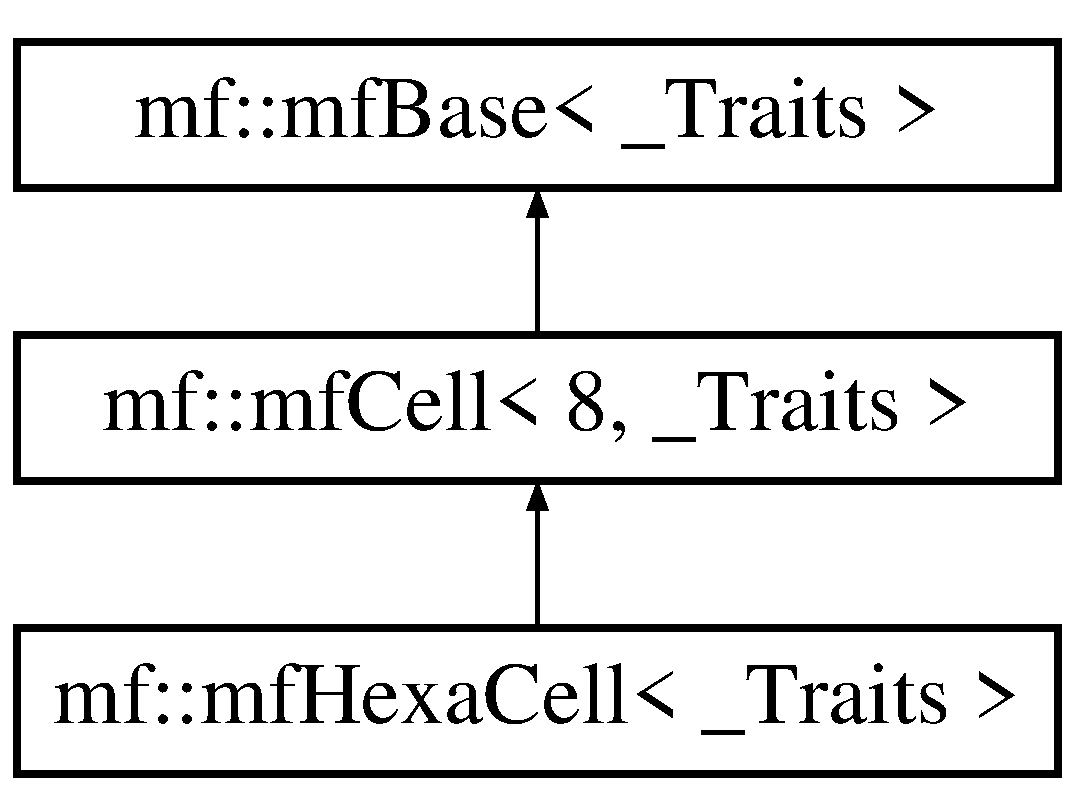
\includegraphics[height=3.000000cm]{classmf_1_1mfHexaCell}
\end{center}
\end{figure}
\subsection*{Public Types}
\begin{DoxyCompactItemize}
\item 
typedef \_\-Traits::ids \hyperlink{classmf_1_1mfHexaCell_a0f1d3a8aa5b31635f48c2d1baa1a9f37}{ids}
\end{DoxyCompactItemize}
\subsection*{Public Member Functions}
\begin{DoxyCompactItemize}
\item 
\hyperlink{classmf_1_1mfBase_a3b23f16ddf59da0a91ab12cf57c1f111}{ids} \hyperlink{classmf_1_1mfHexaCell_a462f9ea4abee25cd3ded82266d04ebd2}{getEdgeId} (int index MF\_\-DMUTEXVD)
\item 
\hypertarget{classmf_1_1mfHexaCell_a3e975d0797cb0c6c4b195835ced52768}{
\hyperlink{classmf_1_1mfBase_a3b23f16ddf59da0a91ab12cf57c1f111}{ids} {\bfseries getEdgeId} (int vIndex1, int vIndex2)}
\label{classmf_1_1mfHexaCell_a3e975d0797cb0c6c4b195835ced52768}

\item 
void \hyperlink{classmf_1_1mfHexaCell_abb7037b42074eaaab7c5a89806d83a29}{setEdgeId} (int index, \hyperlink{classmf_1_1mfBase_a3b23f16ddf59da0a91ab12cf57c1f111}{ids} edge MF\_\-DMUTEXVD)
\item 
\hyperlink{classmf_1_1mfBase_a3b23f16ddf59da0a91ab12cf57c1f111}{ids} \hyperlink{classmf_1_1mfHexaCell_a42fa61d5e21e646e99c905d20792b9c8}{getMateId} (int index MF\_\-DMUTEXVD)
\item 
int \hyperlink{classmf_1_1mfHexaCell_acdc84e16f19d1cd80f720b513463d887}{getRightFaceIndex} (\hyperlink{classmf_1_1mfBase_a3b23f16ddf59da0a91ab12cf57c1f111}{ids} index1, \hyperlink{classmf_1_1mfBase_a3b23f16ddf59da0a91ab12cf57c1f111}{ids} index2)
\item 
int \hyperlink{classmf_1_1mfHexaCell_a15b1537fa930940f61396aed2a743262}{getLeftFaceIndex} (\hyperlink{classmf_1_1mfBase_a3b23f16ddf59da0a91ab12cf57c1f111}{ids} index1, \hyperlink{classmf_1_1mfBase_a3b23f16ddf59da0a91ab12cf57c1f111}{ids} index2)
\item 
\hypertarget{classmf_1_1mfHexaCell_ae110f1775c1cb6fd09905aba9ff3771d}{
int {\bfseries getFaceIndex} (int v1, int v2, int v3)}
\label{classmf_1_1mfHexaCell_ae110f1775c1cb6fd09905aba9ff3771d}

\item 
bool \hyperlink{classmf_1_1mfHexaCell_a46516a81356a071d6aa1d582f63b4985}{verticesAreAdjacent} (\hyperlink{classmf_1_1mfBase_a3b23f16ddf59da0a91ab12cf57c1f111}{ids} index1, \hyperlink{classmf_1_1mfBase_a3b23f16ddf59da0a91ab12cf57c1f111}{ids} index2)
\item 
void \hyperlink{classmf_1_1mfHexaCell_ab512173b13d97508d23083de414491e9}{setMateId} (int index, \hyperlink{classmf_1_1mfBase_a3b23f16ddf59da0a91ab12cf57c1f111}{ids} cell MF\_\-DMUTEXVD)
\item 
void \hyperlink{classmf_1_1mfHexaCell_a924edba7b4baa1564851a09138c0d542}{clearMates} (MF\_\-DMUTEXD)
\item 
int \hyperlink{classmf_1_1mfHexaCell_ae40ba149ff474250c814bf6c7f3af415}{getMateIndex} (\hyperlink{classmf_1_1mfBase_a3b23f16ddf59da0a91ab12cf57c1f111}{ids} cell MF\_\-DMUTEXVD)
\end{DoxyCompactItemize}
\subsection*{Static Public Member Functions}
\begin{DoxyCompactItemize}
\item 
static int \hyperlink{classmf_1_1mfHexaCell_ab53eff357bcacf391a82031240993a32}{getDimension} ()
\item 
static int \hyperlink{classmf_1_1mfHexaCell_a734a620daad4302ebda00686bcb8bd96}{getNumberVerticesInCell} ()
\item 
static int \hyperlink{classmf_1_1mfHexaCell_a34bda59c389b7e9228fbeb6dadac27c3}{getNumberEdgesInCell} ()
\item 
static int \hyperlink{classmf_1_1mfHexaCell_a87767a2fd440a021e6ae7f15cd1edc17}{getNumberFacesInCell} ()
\end{DoxyCompactItemize}
\subsubsection*{template$<$class \_\-Traits$>$ class mf::mfHexaCell$<$ \_\-Traits $>$}



\subsection{Member Typedef Documentation}
\hypertarget{classmf_1_1mfHexaCell_a0f1d3a8aa5b31635f48c2d1baa1a9f37}{
\index{mf::mfHexaCell@{mf::mfHexaCell}!ids@{ids}}
\index{ids@{ids}!mf::mfHexaCell@{mf::mfHexaCell}}
\subsubsection[{ids}]{\setlength{\rightskip}{0pt plus 5cm}template$<$class \_\-Traits $>$ typedef \_\-Traits ::{\bf ids} {\bf mf::mfHexaCell}$<$ \_\-Traits $>$::{\bf ids}}}
\label{classmf_1_1mfHexaCell_a0f1d3a8aa5b31635f48c2d1baa1a9f37}
Id typename definition 

Reimplemented from \hyperlink{classmf_1_1mfCell_a9e32102899fb1e6b5e95b08a6c71063f}{mf::mfCell$<$ 8, \_\-Traits $>$}.



\subsection{Member Function Documentation}
\hypertarget{classmf_1_1mfHexaCell_a924edba7b4baa1564851a09138c0d542}{
\index{mf::mfHexaCell@{mf::mfHexaCell}!clearMates@{clearMates}}
\index{clearMates@{clearMates}!mf::mfHexaCell@{mf::mfHexaCell}}
\subsubsection[{clearMates}]{\setlength{\rightskip}{0pt plus 5cm}template$<$class \_\-Traits $>$ void {\bf mf::mfHexaCell}$<$ \_\-Traits $>$::clearMates (
\begin{DoxyParamCaption}
\item[{MF\_\-DMUTEXD}]{}
\end{DoxyParamCaption}
)}}
\label{classmf_1_1mfHexaCell_a924edba7b4baa1564851a09138c0d542}
Reset the mate cells ids

Define -\/1 for all positions 

Reimplemented from \hyperlink{classmf_1_1mfCell_ac74f86234370beac5f821333ad1ceb4e}{mf::mfCell$<$ 8, \_\-Traits $>$}.

\hypertarget{classmf_1_1mfHexaCell_ab53eff357bcacf391a82031240993a32}{
\index{mf::mfHexaCell@{mf::mfHexaCell}!getDimension@{getDimension}}
\index{getDimension@{getDimension}!mf::mfHexaCell@{mf::mfHexaCell}}
\subsubsection[{getDimension}]{\setlength{\rightskip}{0pt plus 5cm}template$<$class \_\-Traits $>$ static int {\bf mf::mfHexaCell}$<$ \_\-Traits $>$::getDimension (
\begin{DoxyParamCaption}
{}
\end{DoxyParamCaption}
)\hspace{0.3cm}{\ttfamily  \mbox{[}inline, static\mbox{]}}}}
\label{classmf_1_1mfHexaCell_ab53eff357bcacf391a82031240993a32}
Return the opposite cell id of the specified vertex id


\begin{DoxyParams}{Parameters}
{\em cell,:} & the vertex id Return the opposite vertex id of the specified mate cell id\\
\hline
{\em cell,:} & the mate cell id Return the dimension of this cell \\
\hline
\end{DoxyParams}


Reimplemented from \hyperlink{classmf_1_1mfCell_adca6e1707e9d8487c22b3cd0117791a0}{mf::mfCell$<$ 8, \_\-Traits $>$}.

\hypertarget{classmf_1_1mfHexaCell_a462f9ea4abee25cd3ded82266d04ebd2}{
\index{mf::mfHexaCell@{mf::mfHexaCell}!getEdgeId@{getEdgeId}}
\index{getEdgeId@{getEdgeId}!mf::mfHexaCell@{mf::mfHexaCell}}
\subsubsection[{getEdgeId}]{\setlength{\rightskip}{0pt plus 5cm}template$<$class \_\-Traits $>$ IDS {\bf mf::mfHexaCell}$<$ \_\-Traits $>$::getEdgeId (
\begin{DoxyParamCaption}
\item[{int index}]{MF\_\-DMUTEXVD}
\end{DoxyParamCaption}
)}}
\label{classmf_1_1mfHexaCell_a462f9ea4abee25cd3ded82266d04ebd2}
Return the edge id of the specified index


\begin{DoxyParams}{Parameters}
{\em index,:} & position of edge \\
\hline
\end{DoxyParams}
\hypertarget{classmf_1_1mfHexaCell_a15b1537fa930940f61396aed2a743262}{
\index{mf::mfHexaCell@{mf::mfHexaCell}!getLeftFaceIndex@{getLeftFaceIndex}}
\index{getLeftFaceIndex@{getLeftFaceIndex}!mf::mfHexaCell@{mf::mfHexaCell}}
\subsubsection[{getLeftFaceIndex}]{\setlength{\rightskip}{0pt plus 5cm}template$<$class \_\-Traits $>$ int {\bf mf::mfHexaCell}$<$ \_\-Traits $>$::getLeftFaceIndex (
\begin{DoxyParamCaption}
\item[{{\bf ids}}]{index1, }
\item[{{\bf ids}}]{index2}
\end{DoxyParamCaption}
)}}
\label{classmf_1_1mfHexaCell_a15b1537fa930940f61396aed2a743262}
Returns face index to the left of the edge defined by its 2 vertices


\begin{DoxyParams}{Parameters}
{\em index1,:} & Index of the first vertex of the edge \\
\hline
{\em index2,:} & Index of the second vertex of the edge \\
\hline
\end{DoxyParams}
\begin{DoxyReturn}{Returns}
index of the face 
\end{DoxyReturn}
\hypertarget{classmf_1_1mfHexaCell_a42fa61d5e21e646e99c905d20792b9c8}{
\index{mf::mfHexaCell@{mf::mfHexaCell}!getMateId@{getMateId}}
\index{getMateId@{getMateId}!mf::mfHexaCell@{mf::mfHexaCell}}
\subsubsection[{getMateId}]{\setlength{\rightskip}{0pt plus 5cm}template$<$class \_\-Traits $>$ IDS {\bf mf::mfHexaCell}$<$ \_\-Traits $>$::getMateId (
\begin{DoxyParamCaption}
\item[{int index}]{MF\_\-DMUTEXVD}
\end{DoxyParamCaption}
)}}
\label{classmf_1_1mfHexaCell_a42fa61d5e21e646e99c905d20792b9c8}
Return the mate cell id of the specified index


\begin{DoxyParams}{Parameters}
{\em index,:} & position of mate cell \\
\hline
\end{DoxyParams}


Reimplemented from \hyperlink{classmf_1_1mfCell_a2c5d5cc9f5692d2802f86750c6e9c13f}{mf::mfCell$<$ 8, \_\-Traits $>$}.

\hypertarget{classmf_1_1mfHexaCell_ae40ba149ff474250c814bf6c7f3af415}{
\index{mf::mfHexaCell@{mf::mfHexaCell}!getMateIndex@{getMateIndex}}
\index{getMateIndex@{getMateIndex}!mf::mfHexaCell@{mf::mfHexaCell}}
\subsubsection[{getMateIndex}]{\setlength{\rightskip}{0pt plus 5cm}template$<$class \_\-Traits $>$ int {\bf mf::mfHexaCell}$<$ \_\-Traits $>$::getMateIndex (
\begin{DoxyParamCaption}
\item[{{\bf ids} cell}]{MF\_\-DMUTEXVD}
\end{DoxyParamCaption}
)}}
\label{classmf_1_1mfHexaCell_ae40ba149ff474250c814bf6c7f3af415}
Return the position of the opposite vertex id of the specified mate cell id Return the position of the specified mate cell id


\begin{DoxyParams}{Parameters}
{\em cell,:} & the mate cell id \\
\hline
\end{DoxyParams}


Reimplemented from \hyperlink{classmf_1_1mfCell_ae41581511f86555eaa0ebfb5581f55ea}{mf::mfCell$<$ 8, \_\-Traits $>$}.

\hypertarget{classmf_1_1mfHexaCell_a34bda59c389b7e9228fbeb6dadac27c3}{
\index{mf::mfHexaCell@{mf::mfHexaCell}!getNumberEdgesInCell@{getNumberEdgesInCell}}
\index{getNumberEdgesInCell@{getNumberEdgesInCell}!mf::mfHexaCell@{mf::mfHexaCell}}
\subsubsection[{getNumberEdgesInCell}]{\setlength{\rightskip}{0pt plus 5cm}template$<$class \_\-Traits $>$ static int {\bf mf::mfHexaCell}$<$ \_\-Traits $>$::getNumberEdgesInCell (
\begin{DoxyParamCaption}
{}
\end{DoxyParamCaption}
)\hspace{0.3cm}{\ttfamily  \mbox{[}inline, static\mbox{]}}}}
\label{classmf_1_1mfHexaCell_a34bda59c389b7e9228fbeb6dadac27c3}
Return the number of edges of this cell 

Reimplemented from \hyperlink{classmf_1_1mfCell_a16cc93bf1fa21c95014d000c9750e4a0}{mf::mfCell$<$ 8, \_\-Traits $>$}.

\hypertarget{classmf_1_1mfHexaCell_a87767a2fd440a021e6ae7f15cd1edc17}{
\index{mf::mfHexaCell@{mf::mfHexaCell}!getNumberFacesInCell@{getNumberFacesInCell}}
\index{getNumberFacesInCell@{getNumberFacesInCell}!mf::mfHexaCell@{mf::mfHexaCell}}
\subsubsection[{getNumberFacesInCell}]{\setlength{\rightskip}{0pt plus 5cm}template$<$class \_\-Traits $>$ static int {\bf mf::mfHexaCell}$<$ \_\-Traits $>$::getNumberFacesInCell (
\begin{DoxyParamCaption}
{}
\end{DoxyParamCaption}
)\hspace{0.3cm}{\ttfamily  \mbox{[}inline, static\mbox{]}}}}
\label{classmf_1_1mfHexaCell_a87767a2fd440a021e6ae7f15cd1edc17}
Return the number of faces of this cell \hypertarget{classmf_1_1mfHexaCell_a734a620daad4302ebda00686bcb8bd96}{
\index{mf::mfHexaCell@{mf::mfHexaCell}!getNumberVerticesInCell@{getNumberVerticesInCell}}
\index{getNumberVerticesInCell@{getNumberVerticesInCell}!mf::mfHexaCell@{mf::mfHexaCell}}
\subsubsection[{getNumberVerticesInCell}]{\setlength{\rightskip}{0pt plus 5cm}template$<$class \_\-Traits $>$ static int {\bf mf::mfHexaCell}$<$ \_\-Traits $>$::getNumberVerticesInCell (
\begin{DoxyParamCaption}
{}
\end{DoxyParamCaption}
)\hspace{0.3cm}{\ttfamily  \mbox{[}inline, static\mbox{]}}}}
\label{classmf_1_1mfHexaCell_a734a620daad4302ebda00686bcb8bd96}
Return the number of vertices of this cell 

Reimplemented from \hyperlink{classmf_1_1mfCell_ae5031384bc660f1a804ab6603b8c1a19}{mf::mfCell$<$ 8, \_\-Traits $>$}.

\hypertarget{classmf_1_1mfHexaCell_acdc84e16f19d1cd80f720b513463d887}{
\index{mf::mfHexaCell@{mf::mfHexaCell}!getRightFaceIndex@{getRightFaceIndex}}
\index{getRightFaceIndex@{getRightFaceIndex}!mf::mfHexaCell@{mf::mfHexaCell}}
\subsubsection[{getRightFaceIndex}]{\setlength{\rightskip}{0pt plus 5cm}template$<$class \_\-Traits $>$ int {\bf mf::mfHexaCell}$<$ \_\-Traits $>$::getRightFaceIndex (
\begin{DoxyParamCaption}
\item[{{\bf ids}}]{index1, }
\item[{{\bf ids}}]{index2}
\end{DoxyParamCaption}
)}}
\label{classmf_1_1mfHexaCell_acdc84e16f19d1cd80f720b513463d887}
Returns face index to the right of the edge defined by its 2 vertices


\begin{DoxyParams}{Parameters}
{\em index1,:} & Index of the first vertex of the edge \\
\hline
{\em index2,:} & Index of the second vertex of the edge \\
\hline
\end{DoxyParams}
\begin{DoxyReturn}{Returns}
index of the face 
\end{DoxyReturn}
\hypertarget{classmf_1_1mfHexaCell_abb7037b42074eaaab7c5a89806d83a29}{
\index{mf::mfHexaCell@{mf::mfHexaCell}!setEdgeId@{setEdgeId}}
\index{setEdgeId@{setEdgeId}!mf::mfHexaCell@{mf::mfHexaCell}}
\subsubsection[{setEdgeId}]{\setlength{\rightskip}{0pt plus 5cm}template$<$class \_\-Traits $>$ void {\bf mf::mfHexaCell}$<$ \_\-Traits $>$::setEdgeId (
\begin{DoxyParamCaption}
\item[{int}]{index, }
\item[{{\bf ids} edge}]{MF\_\-DMUTEXVD}
\end{DoxyParamCaption}
)}}
\label{classmf_1_1mfHexaCell_abb7037b42074eaaab7c5a89806d83a29}
Return the mate cell id of the specified index


\begin{DoxyParams}{Parameters}
{\em index,:} & position of mate cell \\
\hline
\end{DoxyParams}
\hypertarget{classmf_1_1mfHexaCell_ab512173b13d97508d23083de414491e9}{
\index{mf::mfHexaCell@{mf::mfHexaCell}!setMateId@{setMateId}}
\index{setMateId@{setMateId}!mf::mfHexaCell@{mf::mfHexaCell}}
\subsubsection[{setMateId}]{\setlength{\rightskip}{0pt plus 5cm}template$<$class \_\-Traits $>$ void {\bf mf::mfHexaCell}$<$ \_\-Traits $>$::setMateId (
\begin{DoxyParamCaption}
\item[{int}]{index, }
\item[{{\bf ids} cell}]{MF\_\-DMUTEXVD}
\end{DoxyParamCaption}
)}}
\label{classmf_1_1mfHexaCell_ab512173b13d97508d23083de414491e9}
Define the mate cell id of the specified index


\begin{DoxyParams}{Parameters}
{\em index,:} & position of mate cell \\
\hline
{\em cell,:} & the mate cell id \\
\hline
\end{DoxyParams}


Reimplemented from \hyperlink{classmf_1_1mfCell_a96fe10c334f74928d220d46c3761f024}{mf::mfCell$<$ 8, \_\-Traits $>$}.

\hypertarget{classmf_1_1mfHexaCell_a46516a81356a071d6aa1d582f63b4985}{
\index{mf::mfHexaCell@{mf::mfHexaCell}!verticesAreAdjacent@{verticesAreAdjacent}}
\index{verticesAreAdjacent@{verticesAreAdjacent}!mf::mfHexaCell@{mf::mfHexaCell}}
\subsubsection[{verticesAreAdjacent}]{\setlength{\rightskip}{0pt plus 5cm}template$<$class \_\-Traits $>$ bool {\bf mf::mfHexaCell}$<$ \_\-Traits $>$::verticesAreAdjacent (
\begin{DoxyParamCaption}
\item[{{\bf ids}}]{index1, }
\item[{{\bf ids}}]{index2}
\end{DoxyParamCaption}
)}}
\label{classmf_1_1mfHexaCell_a46516a81356a071d6aa1d582f63b4985}
Determines if two vertices are adjacent


\begin{DoxyParams}{Parameters}
{\em index1,:} & Index of the first vertex \\
\hline
{\em index2,:} & Index of the second vertex \\
\hline
\end{DoxyParams}


The documentation for this class was generated from the following file:\begin{DoxyCompactItemize}
\item 
\hyperlink{mfHexaCell_8h}{mfHexaCell.h}\end{DoxyCompactItemize}

\hypertarget{classmf_1_1mfHybrid2DCell}{
\section{mf::mfHybrid2DCell$<$ \_\-Traits $>$ Class Template Reference}
\label{classmf_1_1mfHybrid2DCell}\index{mf::mfHybrid2DCell@{mf::mfHybrid2DCell}}
}
Inheritance diagram for mf::mfHybrid2DCell$<$ \_\-Traits $>$:\begin{figure}[H]
\begin{center}
\leavevmode
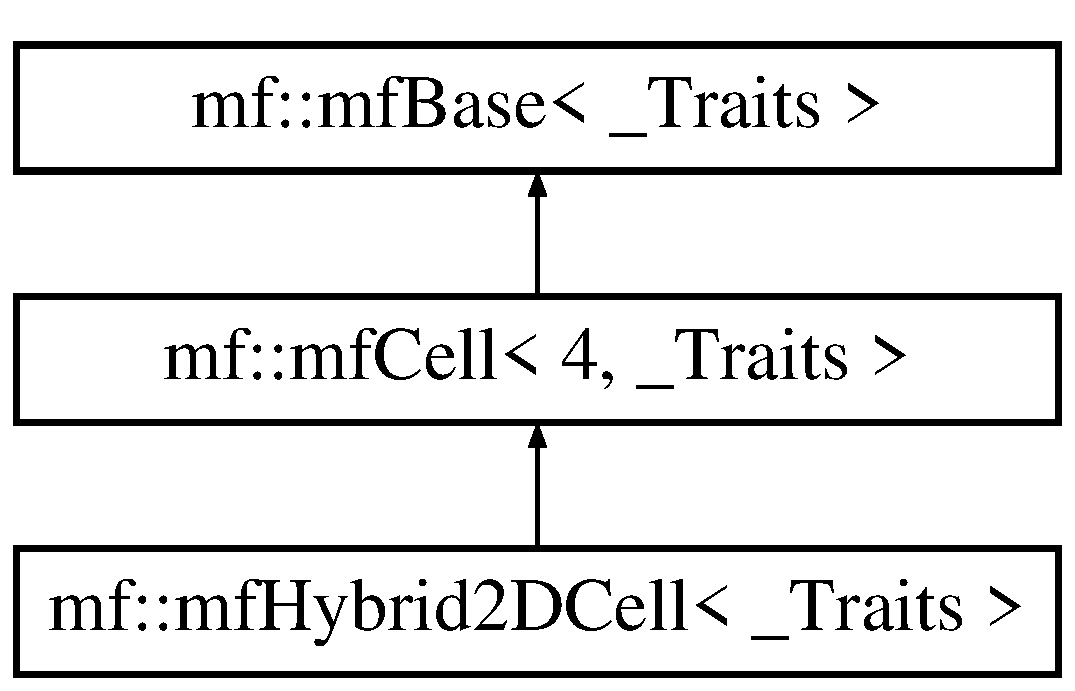
\includegraphics[height=3.000000cm]{classmf_1_1mfHybrid2DCell}
\end{center}
\end{figure}
\subsection*{Public Types}
\begin{DoxyCompactItemize}
\item 
typedef \_\-Traits::ids \hyperlink{classmf_1_1mfHybrid2DCell_a0ee11399531818ab7eac9c5fede19b14}{ids}
\end{DoxyCompactItemize}
\subsection*{Public Member Functions}
\begin{DoxyCompactItemize}
\item 
\hyperlink{classmf_1_1mfHybrid2DCell_a1a8a1a4894a226cd4da0c92ae9e5a41c}{mfHybrid2DCell} ()
\item 
virtual \hyperlink{classmf_1_1mfHybrid2DCell_a83536a3046f0a70ac10cf879b4c8ffe0}{$\sim$mfHybrid2DCell} ()
\item 
\hyperlink{classmf_1_1mfBase_a3b23f16ddf59da0a91ab12cf57c1f111}{ids} \hyperlink{classmf_1_1mfHybrid2DCell_a6c1d59c23b1e25b59196220d3af3a4ef}{getEdgeId} (int index MF\_\-DMUTEXVD)
\item 
void \hyperlink{classmf_1_1mfHybrid2DCell_acf7eaf0c9e4c50f0ac1bb06ca2010250}{setEdgeId} (int index, \hyperlink{classmf_1_1mfBase_a3b23f16ddf59da0a91ab12cf57c1f111}{ids} edge MF\_\-DMUTEXVD)
\item 
int \hyperlink{classmf_1_1mfHybrid2DCell_a0d49a5d889459f5100357c45d192d179}{getNumberVerticesInCell} ()
\item 
int \hyperlink{classmf_1_1mfHybrid2DCell_a717323295b1a993d0c9d029978c84743}{getNumberEdgesInCell} ()
\end{DoxyCompactItemize}
\subsection*{Static Public Member Functions}
\begin{DoxyCompactItemize}
\item 
static int \hyperlink{classmf_1_1mfHybrid2DCell_a93668aada55d3779cfadd32c068eb5e2}{getDimension} ()
\end{DoxyCompactItemize}
\subsubsection*{template$<$class \_\-Traits$>$ class mf::mfHybrid2DCell$<$ \_\-Traits $>$}



\subsection{Member Typedef Documentation}
\hypertarget{classmf_1_1mfHybrid2DCell_a0ee11399531818ab7eac9c5fede19b14}{
\index{mf::mfHybrid2DCell@{mf::mfHybrid2DCell}!ids@{ids}}
\index{ids@{ids}!mf::mfHybrid2DCell@{mf::mfHybrid2DCell}}
\subsubsection[{ids}]{\setlength{\rightskip}{0pt plus 5cm}template$<$class \_\-Traits $>$ typedef \_\-Traits ::{\bf ids} {\bf mf::mfHybrid2DCell}$<$ \_\-Traits $>$::{\bf ids}}}
\label{classmf_1_1mfHybrid2DCell_a0ee11399531818ab7eac9c5fede19b14}
Id typename definition 

Reimplemented from \hyperlink{classmf_1_1mfCell_a9e32102899fb1e6b5e95b08a6c71063f}{mf::mfCell$<$ 4, \_\-Traits $>$}.



\subsection{Constructor \& Destructor Documentation}
\hypertarget{classmf_1_1mfHybrid2DCell_a1a8a1a4894a226cd4da0c92ae9e5a41c}{
\index{mf::mfHybrid2DCell@{mf::mfHybrid2DCell}!mfHybrid2DCell@{mfHybrid2DCell}}
\index{mfHybrid2DCell@{mfHybrid2DCell}!mf::mfHybrid2DCell@{mf::mfHybrid2DCell}}
\subsubsection[{mfHybrid2DCell}]{\setlength{\rightskip}{0pt plus 5cm}template$<$class \_\-Traits $>$ {\bf mf::mfHybrid2DCell}$<$ \_\-Traits $>$::{\bf mfHybrid2DCell} (
\begin{DoxyParamCaption}
{}
\end{DoxyParamCaption}
)}}
\label{classmf_1_1mfHybrid2DCell_a1a8a1a4894a226cd4da0c92ae9e5a41c}
Constructor \hypertarget{classmf_1_1mfHybrid2DCell_a83536a3046f0a70ac10cf879b4c8ffe0}{
\index{mf::mfHybrid2DCell@{mf::mfHybrid2DCell}!$\sim$mfHybrid2DCell@{$\sim$mfHybrid2DCell}}
\index{$\sim$mfHybrid2DCell@{$\sim$mfHybrid2DCell}!mf::mfHybrid2DCell@{mf::mfHybrid2DCell}}
\subsubsection[{$\sim$mfHybrid2DCell}]{\setlength{\rightskip}{0pt plus 5cm}template$<$class \_\-Traits $>$ {\bf mf::mfHybrid2DCell}$<$ \_\-Traits $>$::$\sim${\bf mfHybrid2DCell} (
\begin{DoxyParamCaption}
{}
\end{DoxyParamCaption}
)\hspace{0.3cm}{\ttfamily  \mbox{[}virtual\mbox{]}}}}
\label{classmf_1_1mfHybrid2DCell_a83536a3046f0a70ac10cf879b4c8ffe0}
Destructor 

\subsection{Member Function Documentation}
\hypertarget{classmf_1_1mfHybrid2DCell_a93668aada55d3779cfadd32c068eb5e2}{
\index{mf::mfHybrid2DCell@{mf::mfHybrid2DCell}!getDimension@{getDimension}}
\index{getDimension@{getDimension}!mf::mfHybrid2DCell@{mf::mfHybrid2DCell}}
\subsubsection[{getDimension}]{\setlength{\rightskip}{0pt plus 5cm}template$<$class \_\-Traits $>$ static int {\bf mf::mfHybrid2DCell}$<$ \_\-Traits $>$::getDimension (
\begin{DoxyParamCaption}
{}
\end{DoxyParamCaption}
)\hspace{0.3cm}{\ttfamily  \mbox{[}inline, static\mbox{]}}}}
\label{classmf_1_1mfHybrid2DCell_a93668aada55d3779cfadd32c068eb5e2}
Return the dimension of this cell 

Reimplemented from \hyperlink{classmf_1_1mfCell_adca6e1707e9d8487c22b3cd0117791a0}{mf::mfCell$<$ 4, \_\-Traits $>$}.

\hypertarget{classmf_1_1mfHybrid2DCell_a6c1d59c23b1e25b59196220d3af3a4ef}{
\index{mf::mfHybrid2DCell@{mf::mfHybrid2DCell}!getEdgeId@{getEdgeId}}
\index{getEdgeId@{getEdgeId}!mf::mfHybrid2DCell@{mf::mfHybrid2DCell}}
\subsubsection[{getEdgeId}]{\setlength{\rightskip}{0pt plus 5cm}template$<$class \_\-Traits $>$ IDS {\bf mf::mfHybrid2DCell}$<$ \_\-Traits $>$::getEdgeId (
\begin{DoxyParamCaption}
\item[{int index}]{MF\_\-DMUTEXVD}
\end{DoxyParamCaption}
)}}
\label{classmf_1_1mfHybrid2DCell_a6c1d59c23b1e25b59196220d3af3a4ef}
Return the edge id of the specified index


\begin{DoxyParams}{Parameters}
{\em index,:} & position of edge \\
\hline
\end{DoxyParams}
\hypertarget{classmf_1_1mfHybrid2DCell_a717323295b1a993d0c9d029978c84743}{
\index{mf::mfHybrid2DCell@{mf::mfHybrid2DCell}!getNumberEdgesInCell@{getNumberEdgesInCell}}
\index{getNumberEdgesInCell@{getNumberEdgesInCell}!mf::mfHybrid2DCell@{mf::mfHybrid2DCell}}
\subsubsection[{getNumberEdgesInCell}]{\setlength{\rightskip}{0pt plus 5cm}template$<$class \_\-Traits $>$ int {\bf mf::mfHybrid2DCell}$<$ \_\-Traits $>$::getNumberEdgesInCell (
\begin{DoxyParamCaption}
{}
\end{DoxyParamCaption}
)}}
\label{classmf_1_1mfHybrid2DCell_a717323295b1a993d0c9d029978c84743}
Defines the number of edges of this cell


\begin{DoxyParams}{Parameters}
{\em value,:} & number of edges Return the number of edges of this cell \\
\hline
\end{DoxyParams}


Reimplemented from \hyperlink{classmf_1_1mfCell_a16cc93bf1fa21c95014d000c9750e4a0}{mf::mfCell$<$ 4, \_\-Traits $>$}.

\hypertarget{classmf_1_1mfHybrid2DCell_a0d49a5d889459f5100357c45d192d179}{
\index{mf::mfHybrid2DCell@{mf::mfHybrid2DCell}!getNumberVerticesInCell@{getNumberVerticesInCell}}
\index{getNumberVerticesInCell@{getNumberVerticesInCell}!mf::mfHybrid2DCell@{mf::mfHybrid2DCell}}
\subsubsection[{getNumberVerticesInCell}]{\setlength{\rightskip}{0pt plus 5cm}template$<$class \_\-Traits $>$ int {\bf mf::mfHybrid2DCell}$<$ \_\-Traits $>$::getNumberVerticesInCell (
\begin{DoxyParamCaption}
{}
\end{DoxyParamCaption}
)}}
\label{classmf_1_1mfHybrid2DCell_a0d49a5d889459f5100357c45d192d179}
Defines the number of edges of this cell


\begin{DoxyParams}{Parameters}
{\em value,:} & number of edges Return the number of edges of this cell \\
\hline
\end{DoxyParams}


Reimplemented from \hyperlink{classmf_1_1mfCell_ae5031384bc660f1a804ab6603b8c1a19}{mf::mfCell$<$ 4, \_\-Traits $>$}.

\hypertarget{classmf_1_1mfHybrid2DCell_acf7eaf0c9e4c50f0ac1bb06ca2010250}{
\index{mf::mfHybrid2DCell@{mf::mfHybrid2DCell}!setEdgeId@{setEdgeId}}
\index{setEdgeId@{setEdgeId}!mf::mfHybrid2DCell@{mf::mfHybrid2DCell}}
\subsubsection[{setEdgeId}]{\setlength{\rightskip}{0pt plus 5cm}template$<$class \_\-Traits $>$ void {\bf mf::mfHybrid2DCell}$<$ \_\-Traits $>$::setEdgeId (
\begin{DoxyParamCaption}
\item[{int}]{index, }
\item[{{\bf ids} edge}]{MF\_\-DMUTEXVD}
\end{DoxyParamCaption}
)}}
\label{classmf_1_1mfHybrid2DCell_acf7eaf0c9e4c50f0ac1bb06ca2010250}
Define the edge id of the specified index


\begin{DoxyParams}{Parameters}
{\em index,:} & position of edge \\
\hline
{\em edge,:} & the edge id \\
\hline
\end{DoxyParams}


The documentation for this class was generated from the following file:\begin{DoxyCompactItemize}
\item 
\hyperlink{mfHybrid2DCell_8h}{mfHybrid2DCell.h}\end{DoxyCompactItemize}

\hypertarget{classmf_1_1mfHybridCell}{
\section{mf::mfHybridCell$<$ \_\-Traits $>$ Class Template Reference}
\label{classmf_1_1mfHybridCell}\index{mf::mfHybridCell@{mf::mfHybridCell}}
}


{\ttfamily \#include $<$mfHybridCell.h$>$}

Inheritance diagram for mf::mfHybridCell$<$ \_\-Traits $>$:\begin{figure}[H]
\begin{center}
\leavevmode
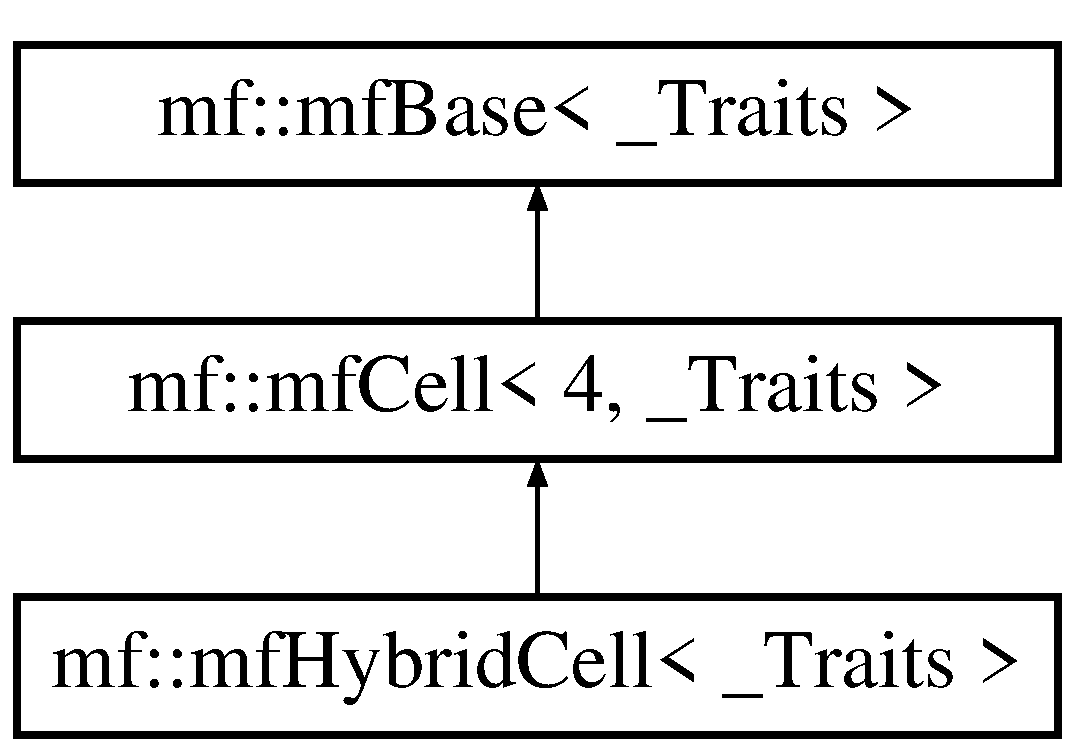
\includegraphics[height=3.000000cm]{classmf_1_1mfHybridCell}
\end{center}
\end{figure}
\subsection*{Public Types}
\begin{DoxyCompactItemize}
\item 
typedef \_\-Traits::ids \hyperlink{classmf_1_1mfHybridCell_afcc1603f9fd31f5e82fc0f2175aa74d2}{ids}
\end{DoxyCompactItemize}
\subsection*{Public Member Functions}
\begin{DoxyCompactItemize}
\item 
\hyperlink{classmf_1_1mfHybridCell_a526117a90df3cb8a4413836848da8075}{mfHybridCell} ()
\item 
virtual \hyperlink{classmf_1_1mfHybridCell_a228b2863f54124331dda1666afad420b}{$\sim$mfHybridCell} ()
\item 
\hyperlink{classmf_1_1mfBase_a3b23f16ddf59da0a91ab12cf57c1f111}{ids} \hyperlink{classmf_1_1mfHybridCell_ab58d17515251ea065b1b54f32a91fb72}{getEdgeId} (int index MF\_\-DMUTEXVD)
\item 
void \hyperlink{classmf_1_1mfHybridCell_a45b53202d66076c7b9227b5f4897a0ed}{setEdgeId} (int index, \hyperlink{classmf_1_1mfBase_a3b23f16ddf59da0a91ab12cf57c1f111}{ids} edge MF\_\-DMUTEXVD)
\item 
int \hyperlink{classmf_1_1mfHybridCell_a39449ac79227d63f7cf505305ceb89d0}{getNumberVerticesInCell} ()
\item 
int \hyperlink{classmf_1_1mfHybridCell_a5fc9ef1bea17984822cf28d0ed6dde20}{getNumberEdgesInCell} ()
\end{DoxyCompactItemize}
\subsection*{Static Public Member Functions}
\begin{DoxyCompactItemize}
\item 
static int \hyperlink{classmf_1_1mfHybridCell_a4fb353f76e3fd38febcf2f71c1e11d76}{getDimension} ()
\end{DoxyCompactItemize}


\subsection{Detailed Description}
\subsubsection*{template$<$class \_\-Traits$>$ class mf::mfHybridCell$<$ \_\-Traits $>$}

Base class of triangle 

\subsection{Member Typedef Documentation}
\hypertarget{classmf_1_1mfHybridCell_afcc1603f9fd31f5e82fc0f2175aa74d2}{
\index{mf::mfHybridCell@{mf::mfHybridCell}!ids@{ids}}
\index{ids@{ids}!mf::mfHybridCell@{mf::mfHybridCell}}
\subsubsection[{ids}]{\setlength{\rightskip}{0pt plus 5cm}template$<$class \_\-Traits $>$ typedef \_\-Traits ::{\bf ids} {\bf mf::mfHybridCell}$<$ \_\-Traits $>$::{\bf ids}}}
\label{classmf_1_1mfHybridCell_afcc1603f9fd31f5e82fc0f2175aa74d2}
Id typename definition 

Reimplemented from \hyperlink{classmf_1_1mfCell_a9e32102899fb1e6b5e95b08a6c71063f}{mf::mfCell$<$ 4, \_\-Traits $>$}.



\subsection{Constructor \& Destructor Documentation}
\hypertarget{classmf_1_1mfHybridCell_a526117a90df3cb8a4413836848da8075}{
\index{mf::mfHybridCell@{mf::mfHybridCell}!mfHybridCell@{mfHybridCell}}
\index{mfHybridCell@{mfHybridCell}!mf::mfHybridCell@{mf::mfHybridCell}}
\subsubsection[{mfHybridCell}]{\setlength{\rightskip}{0pt plus 5cm}template$<$class \_\-Traits $>$ {\bf mf::mfHybridCell}$<$ \_\-Traits $>$::{\bf mfHybridCell} (
\begin{DoxyParamCaption}
{}
\end{DoxyParamCaption}
)}}
\label{classmf_1_1mfHybridCell_a526117a90df3cb8a4413836848da8075}
Constructor \hypertarget{classmf_1_1mfHybridCell_a228b2863f54124331dda1666afad420b}{
\index{mf::mfHybridCell@{mf::mfHybridCell}!$\sim$mfHybridCell@{$\sim$mfHybridCell}}
\index{$\sim$mfHybridCell@{$\sim$mfHybridCell}!mf::mfHybridCell@{mf::mfHybridCell}}
\subsubsection[{$\sim$mfHybridCell}]{\setlength{\rightskip}{0pt plus 5cm}template$<$class \_\-Traits $>$ {\bf mf::mfHybridCell}$<$ \_\-Traits $>$::$\sim${\bf mfHybridCell} (
\begin{DoxyParamCaption}
{}
\end{DoxyParamCaption}
)\hspace{0.3cm}{\ttfamily  \mbox{[}virtual\mbox{]}}}}
\label{classmf_1_1mfHybridCell_a228b2863f54124331dda1666afad420b}
Destructor 

\subsection{Member Function Documentation}
\hypertarget{classmf_1_1mfHybridCell_a4fb353f76e3fd38febcf2f71c1e11d76}{
\index{mf::mfHybridCell@{mf::mfHybridCell}!getDimension@{getDimension}}
\index{getDimension@{getDimension}!mf::mfHybridCell@{mf::mfHybridCell}}
\subsubsection[{getDimension}]{\setlength{\rightskip}{0pt plus 5cm}template$<$class \_\-Traits $>$ static int {\bf mf::mfHybridCell}$<$ \_\-Traits $>$::getDimension (
\begin{DoxyParamCaption}
{}
\end{DoxyParamCaption}
)\hspace{0.3cm}{\ttfamily  \mbox{[}inline, static\mbox{]}}}}
\label{classmf_1_1mfHybridCell_a4fb353f76e3fd38febcf2f71c1e11d76}
Return the dimension of this cell 

Reimplemented from \hyperlink{classmf_1_1mfCell_adca6e1707e9d8487c22b3cd0117791a0}{mf::mfCell$<$ 4, \_\-Traits $>$}.

\hypertarget{classmf_1_1mfHybridCell_ab58d17515251ea065b1b54f32a91fb72}{
\index{mf::mfHybridCell@{mf::mfHybridCell}!getEdgeId@{getEdgeId}}
\index{getEdgeId@{getEdgeId}!mf::mfHybridCell@{mf::mfHybridCell}}
\subsubsection[{getEdgeId}]{\setlength{\rightskip}{0pt plus 5cm}template$<$class \_\-Traits $>$ IDS {\bf mf::mfHybridCell}$<$ \_\-Traits $>$::getEdgeId (
\begin{DoxyParamCaption}
\item[{int index}]{MF\_\-DMUTEXVD}
\end{DoxyParamCaption}
)}}
\label{classmf_1_1mfHybridCell_ab58d17515251ea065b1b54f32a91fb72}
Return the edge id of the specified index


\begin{DoxyParams}{Parameters}
{\em index,:} & position of edge \\
\hline
\end{DoxyParams}
\hypertarget{classmf_1_1mfHybridCell_a5fc9ef1bea17984822cf28d0ed6dde20}{
\index{mf::mfHybridCell@{mf::mfHybridCell}!getNumberEdgesInCell@{getNumberEdgesInCell}}
\index{getNumberEdgesInCell@{getNumberEdgesInCell}!mf::mfHybridCell@{mf::mfHybridCell}}
\subsubsection[{getNumberEdgesInCell}]{\setlength{\rightskip}{0pt plus 5cm}template$<$class \_\-Traits $>$ int {\bf mf::mfHybridCell}$<$ \_\-Traits $>$::getNumberEdgesInCell (
\begin{DoxyParamCaption}
{}
\end{DoxyParamCaption}
)}}
\label{classmf_1_1mfHybridCell_a5fc9ef1bea17984822cf28d0ed6dde20}
Defines the number of edges of this cell


\begin{DoxyParams}{Parameters}
{\em value,:} & number of edges Return the number of edges of this cell \\
\hline
\end{DoxyParams}


Reimplemented from \hyperlink{classmf_1_1mfCell_a16cc93bf1fa21c95014d000c9750e4a0}{mf::mfCell$<$ 4, \_\-Traits $>$}.

\hypertarget{classmf_1_1mfHybridCell_a39449ac79227d63f7cf505305ceb89d0}{
\index{mf::mfHybridCell@{mf::mfHybridCell}!getNumberVerticesInCell@{getNumberVerticesInCell}}
\index{getNumberVerticesInCell@{getNumberVerticesInCell}!mf::mfHybridCell@{mf::mfHybridCell}}
\subsubsection[{getNumberVerticesInCell}]{\setlength{\rightskip}{0pt plus 5cm}template$<$class \_\-Traits $>$ int {\bf mf::mfHybridCell}$<$ \_\-Traits $>$::getNumberVerticesInCell (
\begin{DoxyParamCaption}
{}
\end{DoxyParamCaption}
)}}
\label{classmf_1_1mfHybridCell_a39449ac79227d63f7cf505305ceb89d0}
Defines the number of edges of this cell


\begin{DoxyParams}{Parameters}
{\em value,:} & number of edges Return the number of edges of this cell \\
\hline
\end{DoxyParams}


Reimplemented from \hyperlink{classmf_1_1mfCell_ae5031384bc660f1a804ab6603b8c1a19}{mf::mfCell$<$ 4, \_\-Traits $>$}.

\hypertarget{classmf_1_1mfHybridCell_a45b53202d66076c7b9227b5f4897a0ed}{
\index{mf::mfHybridCell@{mf::mfHybridCell}!setEdgeId@{setEdgeId}}
\index{setEdgeId@{setEdgeId}!mf::mfHybridCell@{mf::mfHybridCell}}
\subsubsection[{setEdgeId}]{\setlength{\rightskip}{0pt plus 5cm}template$<$class \_\-Traits $>$ void {\bf mf::mfHybridCell}$<$ \_\-Traits $>$::setEdgeId (
\begin{DoxyParamCaption}
\item[{int}]{index, }
\item[{{\bf ids} edge}]{MF\_\-DMUTEXVD}
\end{DoxyParamCaption}
)}}
\label{classmf_1_1mfHybridCell_a45b53202d66076c7b9227b5f4897a0ed}
Define the edge id of the specified index


\begin{DoxyParams}{Parameters}
{\em index,:} & position of edge \\
\hline
{\em edge,:} & the edge id \\
\hline
\end{DoxyParams}


The documentation for this class was generated from the following file:\begin{DoxyCompactItemize}
\item 
mfHybridCell.h\end{DoxyCompactItemize}

\hypertarget{classmf_1_1mfIterator}{
\section{mf::mfIterator$<$ \_\-Traits $>$ Class Template Reference}
\label{classmf_1_1mfIterator}\index{mf::mfIterator@{mf::mfIterator}}
}
Inheritance diagram for mf::mfIterator$<$ \_\-Traits $>$:\begin{figure}[H]
\begin{center}
\leavevmode
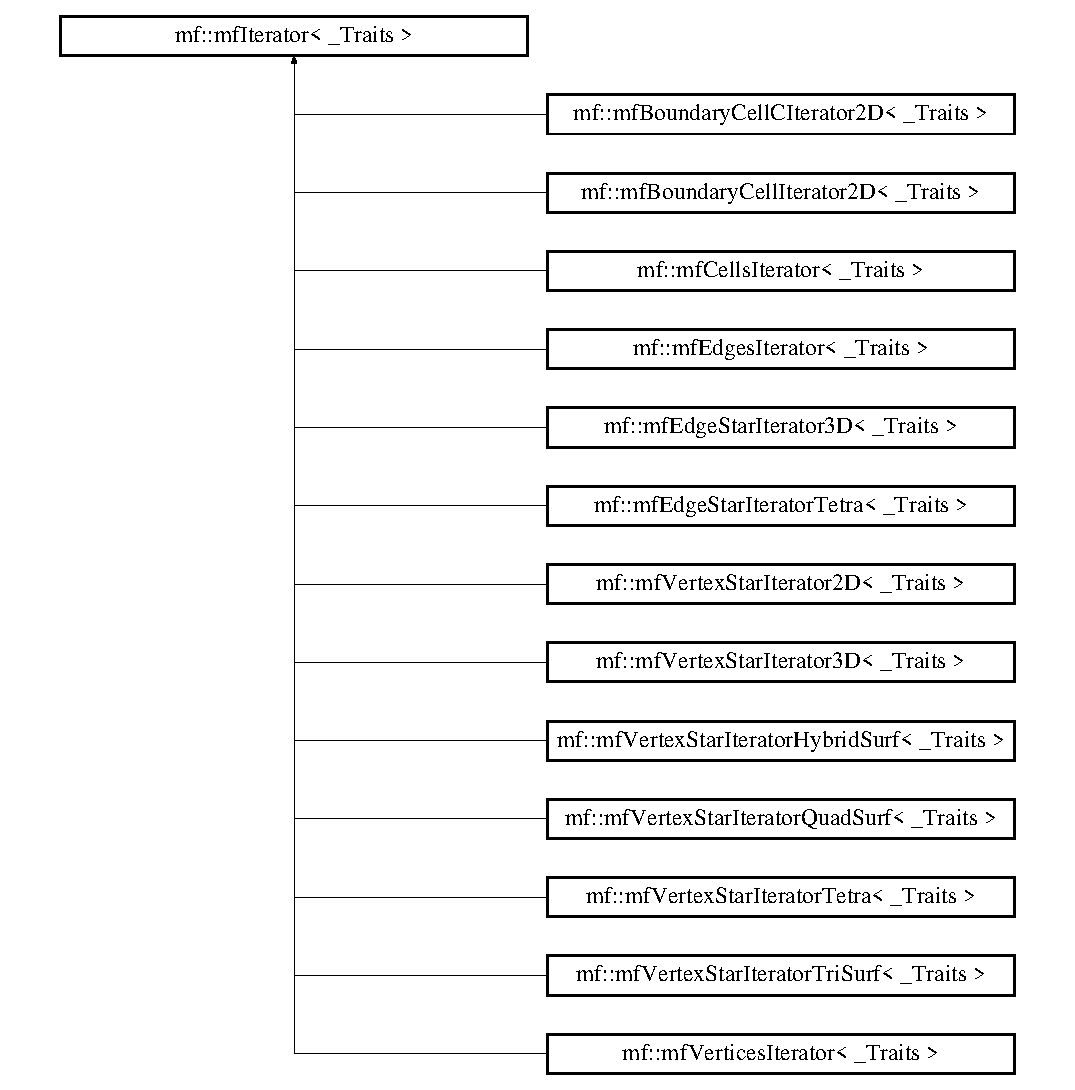
\includegraphics[height=12.000000cm]{classmf_1_1mfIterator}
\end{center}
\end{figure}
\subsection*{Public Types}
\begin{DoxyCompactItemize}
\item 
typedef \_\-Traits::sMesh \hyperlink{classmf_1_1mfIterator_aca31e4d7e7eca4e3b100530d8725064b}{sMesh}
\end{DoxyCompactItemize}
\subsection*{Public Member Functions}
\begin{DoxyCompactItemize}
\item 
void \hyperlink{classmf_1_1mfIterator_aae09ea9494442bf0a634d6d1d4cc7375}{setMesh} (\hyperlink{classmf_1_1mfIterator_aca31e4d7e7eca4e3b100530d8725064b}{sMesh} $\ast$\_\-mesh)
\end{DoxyCompactItemize}
\subsection*{Protected Member Functions}
\begin{DoxyCompactItemize}
\item 
\hyperlink{classmf_1_1mfIterator_a449e71efbd66d915eb9fb9be7de1b9ca}{mfIterator} (\hyperlink{classmf_1_1mfIterator_aca31e4d7e7eca4e3b100530d8725064b}{sMesh} $\ast$\_\-mesh)
\item 
\hyperlink{classmf_1_1mfIterator_abf1ee78fa042174107d215ba0da8bc8f}{$\sim$mfIterator} ()
\end{DoxyCompactItemize}
\subsection*{Protected Attributes}
\begin{DoxyCompactItemize}
\item 
\hyperlink{classmf_1_1mfIterator_aca31e4d7e7eca4e3b100530d8725064b}{sMesh} $\ast$ \hyperlink{classmf_1_1mfIterator_a605ced32b4a7f8a90a3cc947d9cd431b}{mesh}
\end{DoxyCompactItemize}
\subsubsection*{template$<$class \_\-Traits$>$ class mf::mfIterator$<$ \_\-Traits $>$}



\subsection{Member Typedef Documentation}
\hypertarget{classmf_1_1mfIterator_aca31e4d7e7eca4e3b100530d8725064b}{
\index{mf::mfIterator@{mf::mfIterator}!sMesh@{sMesh}}
\index{sMesh@{sMesh}!mf::mfIterator@{mf::mfIterator}}
\subsubsection[{sMesh}]{\setlength{\rightskip}{0pt plus 5cm}template$<$class \_\-Traits $>$ typedef \_\-Traits::sMesh {\bf mf::mfIterator}$<$ \_\-Traits $>$::{\bf sMesh}}}
\label{classmf_1_1mfIterator_aca31e4d7e7eca4e3b100530d8725064b}
Mesh typename definition 

Reimplemented in \hyperlink{classmf_1_1mfBoundaryCellCIterator2D_a7cd4a533656715c1768db299fbd3e738}{mf::mfBoundaryCellCIterator2D$<$ \_\-Traits $>$}, \hyperlink{classmf_1_1mfBoundaryCellIterator2D_a4a2bc693e6241fee66020dd32ae7115e}{mf::mfBoundaryCellIterator2D$<$ \_\-Traits $>$}, \hyperlink{classmf_1_1mfCellsIterator_a3f16876b669a93e719af84cdc0c9dad9}{mf::mfCellsIterator$<$ \_\-Traits $>$}, \hyperlink{classmf_1_1mfEdgesIterator_aef5fcd1a83c753089ba7c4e3d6f33733}{mf::mfEdgesIterator$<$ \_\-Traits $>$}, \hyperlink{classmf_1_1mfEdgeStarIterator3D_a875ac7316bdc779e38b0a8befde57366}{mf::mfEdgeStarIterator3D$<$ \_\-Traits $>$}, \hyperlink{classmf_1_1mfEdgeStarIteratorTetra_abbb7ca848037b976d69368943567397b}{mf::mfEdgeStarIteratorTetra$<$ \_\-Traits $>$}, \hyperlink{classmf_1_1mfVertexStarIterator2D_a25f97b24c35482b8677e4672d70687cf}{mf::mfVertexStarIterator2D$<$ \_\-Traits $>$}, \hyperlink{classmf_1_1mfVertexStarIterator3D_aa45e0318e1153d3b373ec69af44d6710}{mf::mfVertexStarIterator3D$<$ \_\-Traits $>$}, \hyperlink{classmf_1_1mfVertexStarIteratorHybridSurf_a83c02395712edc51c7887c7256718c2c}{mf::mfVertexStarIteratorHybridSurf$<$ \_\-Traits $>$}, \hyperlink{classmf_1_1mfVertexStarIteratorQuadSurf_aad751ed48afa8c48bba2ed997bdd4676}{mf::mfVertexStarIteratorQuadSurf$<$ \_\-Traits $>$}, \hyperlink{classmf_1_1mfVertexStarIteratorTetra_a19a9aafec3afbbafea712fa9c1a3417e}{mf::mfVertexStarIteratorTetra$<$ \_\-Traits $>$}, \hyperlink{classmf_1_1mfVertexStarIteratorTriSurf_a6a0a8773d65d971e636d4361fb65b5af}{mf::mfVertexStarIteratorTriSurf$<$ \_\-Traits $>$}, and \hyperlink{classmf_1_1mfVerticesIterator_a351a7fef8c19f4cb57f4c0a68d337679}{mf::mfVerticesIterator$<$ \_\-Traits $>$}.



\subsection{Constructor \& Destructor Documentation}
\hypertarget{classmf_1_1mfIterator_a449e71efbd66d915eb9fb9be7de1b9ca}{
\index{mf::mfIterator@{mf::mfIterator}!mfIterator@{mfIterator}}
\index{mfIterator@{mfIterator}!mf::mfIterator@{mf::mfIterator}}
\subsubsection[{mfIterator}]{\setlength{\rightskip}{0pt plus 5cm}template$<$class \_\-Traits $>$ {\bf mf::mfIterator}$<$ \_\-Traits $>$::{\bf mfIterator} (
\begin{DoxyParamCaption}
\item[{{\bf sMesh} $\ast$}]{\_\-mesh}
\end{DoxyParamCaption}
)\hspace{0.3cm}{\ttfamily  \mbox{[}protected\mbox{]}}}}
\label{classmf_1_1mfIterator_a449e71efbd66d915eb9fb9be7de1b9ca}
Constructor


\begin{DoxyParams}{Parameters}
{\em \_\-mesh,:} & the mesh instance that this class will manipulate \\
\hline
\end{DoxyParams}
\hypertarget{classmf_1_1mfIterator_abf1ee78fa042174107d215ba0da8bc8f}{
\index{mf::mfIterator@{mf::mfIterator}!$\sim$mfIterator@{$\sim$mfIterator}}
\index{$\sim$mfIterator@{$\sim$mfIterator}!mf::mfIterator@{mf::mfIterator}}
\subsubsection[{$\sim$mfIterator}]{\setlength{\rightskip}{0pt plus 5cm}template$<$class \_\-Traits $>$ {\bf mf::mfIterator}$<$ \_\-Traits $>$::$\sim${\bf mfIterator} (
\begin{DoxyParamCaption}
{}
\end{DoxyParamCaption}
)\hspace{0.3cm}{\ttfamily  \mbox{[}protected\mbox{]}}}}
\label{classmf_1_1mfIterator_abf1ee78fa042174107d215ba0da8bc8f}
Destrutor 

\subsection{Member Function Documentation}
\hypertarget{classmf_1_1mfIterator_aae09ea9494442bf0a634d6d1d4cc7375}{
\index{mf::mfIterator@{mf::mfIterator}!setMesh@{setMesh}}
\index{setMesh@{setMesh}!mf::mfIterator@{mf::mfIterator}}
\subsubsection[{setMesh}]{\setlength{\rightskip}{0pt plus 5cm}template$<$class \_\-Traits $>$ void {\bf mf::mfIterator}$<$ \_\-Traits $>$::setMesh (
\begin{DoxyParamCaption}
\item[{{\bf sMesh} $\ast$}]{\_\-mesh}
\end{DoxyParamCaption}
)}}
\label{classmf_1_1mfIterator_aae09ea9494442bf0a634d6d1d4cc7375}
Set the mesh instance to which this class will manipulate.


\begin{DoxyParams}{Parameters}
{\em \_\-mesh,:} & the mesh address that this class will manipulate \\
\hline
\end{DoxyParams}


\subsection{Member Data Documentation}
\hypertarget{classmf_1_1mfIterator_a605ced32b4a7f8a90a3cc947d9cd431b}{
\index{mf::mfIterator@{mf::mfIterator}!mesh@{mesh}}
\index{mesh@{mesh}!mf::mfIterator@{mf::mfIterator}}
\subsubsection[{mesh}]{\setlength{\rightskip}{0pt plus 5cm}template$<$class \_\-Traits $>$ {\bf sMesh}$\ast$ {\bf mf::mfIterator}$<$ \_\-Traits $>$::{\bf mesh}\hspace{0.3cm}{\ttfamily  \mbox{[}protected\mbox{]}}}}
\label{classmf_1_1mfIterator_a605ced32b4a7f8a90a3cc947d9cd431b}
The mesh that this class will manipulate 

The documentation for this class was generated from the following file:\begin{DoxyCompactItemize}
\item 
\hyperlink{mfIterator_8h}{mfIterator.h}\end{DoxyCompactItemize}

\hypertarget{classmf_1_1mfKdTree}{
\section{mf::mfKdTree$<$ sObject, sObjectCompare $>$ Class Template Reference}
\label{classmf_1_1mfKdTree}\index{mf::mfKdTree@{mf::mfKdTree}}
}
\subsection*{Public Member Functions}
\begin{DoxyCompactItemize}
\item 
\hyperlink{classmf_1_1mfKdTree_a0b1cf7f08b3021060bfbec20a48b9b3b}{mfKdTree} (int dim)
\item 
\hyperlink{classmf_1_1mfKdTree_a237a36fe0226ed522ddfc5d4a7f3a8b8}{$\sim$mfKdTree} ()
\item 
\hypertarget{classmf_1_1mfKdTree_abea779a2059a7c535a89fc7e4baef307}{
void {\bfseries insert} (sObject obj)}
\label{classmf_1_1mfKdTree_abea779a2059a7c535a89fc7e4baef307}

\item 
\hypertarget{classmf_1_1mfKdTree_afa8778cfee34a06d8b9b2ba2ceb31cb0}{
sObject {\bfseries nearest} (sObject obj)}
\label{classmf_1_1mfKdTree_afa8778cfee34a06d8b9b2ba2ceb31cb0}

\item 
\hypertarget{classmf_1_1mfKdTree_a6cbc124706ac07e2d5562ad6bf7f7d3b}{
sObject {\bfseries nearestAndInsert} (sObject obj)}
\label{classmf_1_1mfKdTree_a6cbc124706ac07e2d5562ad6bf7f7d3b}

\item 
\hypertarget{classmf_1_1mfKdTree_aede67ecedd3fad76b47d5d988e667b41}{
int {\bfseries size} ()}
\label{classmf_1_1mfKdTree_aede67ecedd3fad76b47d5d988e667b41}

\end{DoxyCompactItemize}
\subsubsection*{template$<$class sObject, class sObjectCompare$>$ class mf::mfKdTree$<$ sObject, sObjectCompare $>$}



\subsection{Constructor \& Destructor Documentation}
\hypertarget{classmf_1_1mfKdTree_a0b1cf7f08b3021060bfbec20a48b9b3b}{
\index{mf::mfKdTree@{mf::mfKdTree}!mfKdTree@{mfKdTree}}
\index{mfKdTree@{mfKdTree}!mf::mfKdTree@{mf::mfKdTree}}
\subsubsection[{mfKdTree}]{\setlength{\rightskip}{0pt plus 5cm}template$<$class sObject , class sObjectCompare $>$ {\bf mf::mfKdTree}$<$ sObject, sObjectCompare $>$::{\bf mfKdTree} (
\begin{DoxyParamCaption}
\item[{int}]{dim}
\end{DoxyParamCaption}
)}}
\label{classmf_1_1mfKdTree_a0b1cf7f08b3021060bfbec20a48b9b3b}
Constructor \hypertarget{classmf_1_1mfKdTree_a237a36fe0226ed522ddfc5d4a7f3a8b8}{
\index{mf::mfKdTree@{mf::mfKdTree}!$\sim$mfKdTree@{$\sim$mfKdTree}}
\index{$\sim$mfKdTree@{$\sim$mfKdTree}!mf::mfKdTree@{mf::mfKdTree}}
\subsubsection[{$\sim$mfKdTree}]{\setlength{\rightskip}{0pt plus 5cm}template$<$class sObject , class sObjectCompare $>$ {\bf mf::mfKdTree}$<$ sObject, sObjectCompare $>$::$\sim${\bf mfKdTree} (
\begin{DoxyParamCaption}
{}
\end{DoxyParamCaption}
)}}
\label{classmf_1_1mfKdTree_a237a36fe0226ed522ddfc5d4a7f3a8b8}
Destructor 

The documentation for this class was generated from the following file:\begin{DoxyCompactItemize}
\item 
mfKdTree.h\end{DoxyCompactItemize}

\hypertarget{structmf_1_1mfKdTreeNode}{
\section{mf::mfKdTreeNode$<$ sObject $>$ Struct Template Reference}
\label{structmf_1_1mfKdTreeNode}\index{mf::mfKdTreeNode@{mf::mfKdTreeNode}}
}
\subsection*{Public Attributes}
\begin{DoxyCompactItemize}
\item 
\hypertarget{structmf_1_1mfKdTreeNode_aa586026f4826ae7ad48607f3b89ead0c}{
sObject {\bfseries ptr}}
\label{structmf_1_1mfKdTreeNode_aa586026f4826ae7ad48607f3b89ead0c}

\item 
\hypertarget{structmf_1_1mfKdTreeNode_a6e7b460c40df90703d89ab771cec182a}{
\hyperlink{structmf_1_1mfKdTreeNode}{mfKdTreeNode} $\ast$ {\bfseries p} \mbox{[}2\mbox{]}}
\label{structmf_1_1mfKdTreeNode_a6e7b460c40df90703d89ab771cec182a}

\end{DoxyCompactItemize}
\subsubsection*{template$<$class sObject$>$ struct mf::mfKdTreeNode$<$ sObject $>$}



The documentation for this struct was generated from the following file:\begin{DoxyCompactItemize}
\item 
mfKdTree.h\end{DoxyCompactItemize}

\hypertarget{classmf_1_1mfList}{
\section{mf::mfList$<$ T $>$ Class Template Reference}
\label{classmf_1_1mfList}\index{mf::mfList@{mf::mfList}}
}
\subsection*{Public Member Functions}
\begin{DoxyCompactItemize}
\item 
\hyperlink{classmf_1_1mfList_a9dd33ef36055bea004031002d4a4f026}{mfList} ()
\item 
\hyperlink{classmf_1_1mfList_ad4d3eec9f511b150164eec42459ca134}{$\sim$mfList} ()
\item 
T \hyperlink{classmf_1_1mfList_a847bb77a327152d37cedb7cc67bb0a15}{pos} (int pos)
\item 
T \hyperlink{classmf_1_1mfList_aa4aa1f0cadb360d2a30b020c0f033d6b}{first} ()
\item 
T \hyperlink{classmf_1_1mfList_a9cfc645e054d48f9b0f59e071d7b24c2}{last} ()
\item 
int \hyperlink{classmf_1_1mfList_a46420521581b1d1786feec1d220d13a0}{size} ()
\item 
void \hyperlink{classmf_1_1mfList_aa6109befcbdbfa250c92ac64f158356f}{insert} (T novo)
\item 
bool \hyperlink{classmf_1_1mfList_a06c516722437afbea46d194ee69f405c}{insertOnlyOne} (T novo)
\item 
void \hyperlink{classmf_1_1mfList_aa674ce8284228bf3840da51237b36490}{insertFirst} (T novo)
\item 
void \hyperlink{classmf_1_1mfList_a9e4631c431e66facd94f5118a057125a}{insert} (T novo, int pos)
\item 
bool \hyperlink{classmf_1_1mfList_ab8b24b126809bfdfad4dc9bff662de32}{erase} (int pos)
\item 
bool \hyperlink{classmf_1_1mfList_a99299b5d36f398ccb0becf383c7364ed}{inList} (T info)
\item 
int \hyperlink{classmf_1_1mfList_a1a43deefc120cb65083011dd6202a5d9}{search} (T info)
\item 
void \hyperlink{classmf_1_1mfList_aba45770f50fda9994f9a32aff96bc410}{clear} ()
\item 
bool \hyperlink{classmf_1_1mfList_ae12dd483320f7d90846e3f8af843244c}{empty} ()
\end{DoxyCompactItemize}
\subsection*{Protected Attributes}
\begin{DoxyCompactItemize}
\item 
int \hyperlink{classmf_1_1mfList_a05d51ad01af004b129160206f8434ff9}{lsize}
\item 
\hyperlink{classmf_1_1mfListNode}{mfListNode}$<$ T $>$ $\ast$ \hyperlink{classmf_1_1mfList_a814cc8674a44ba839f7cbbcc6a4bb172}{lfirst}
\item 
\hyperlink{classmf_1_1mfListNode}{mfListNode}$<$ T $>$ $\ast$ \hyperlink{classmf_1_1mfList_a5c24c5c4cf0d4807f181cf9ae36dd028}{llast}
\end{DoxyCompactItemize}
\subsubsection*{template$<$class T$>$ class mf::mfList$<$ T $>$}



\subsection{Constructor \& Destructor Documentation}
\hypertarget{classmf_1_1mfList_a9dd33ef36055bea004031002d4a4f026}{
\index{mf::mfList@{mf::mfList}!mfList@{mfList}}
\index{mfList@{mfList}!mf::mfList@{mf::mfList}}
\subsubsection[{mfList}]{\setlength{\rightskip}{0pt plus 5cm}template$<$class T $>$ {\bf mf::mfList}$<$ T $>$::{\bf mfList} (
\begin{DoxyParamCaption}
{}
\end{DoxyParamCaption}
)}}
\label{classmf_1_1mfList_a9dd33ef36055bea004031002d4a4f026}
Constructor \hypertarget{classmf_1_1mfList_ad4d3eec9f511b150164eec42459ca134}{
\index{mf::mfList@{mf::mfList}!$\sim$mfList@{$\sim$mfList}}
\index{$\sim$mfList@{$\sim$mfList}!mf::mfList@{mf::mfList}}
\subsubsection[{$\sim$mfList}]{\setlength{\rightskip}{0pt plus 5cm}template$<$class T $>$ {\bf mf::mfList}$<$ T $>$::$\sim${\bf mfList} (
\begin{DoxyParamCaption}
{}
\end{DoxyParamCaption}
)}}
\label{classmf_1_1mfList_ad4d3eec9f511b150164eec42459ca134}
Destructor 

\subsection{Member Function Documentation}
\hypertarget{classmf_1_1mfList_aba45770f50fda9994f9a32aff96bc410}{
\index{mf::mfList@{mf::mfList}!clear@{clear}}
\index{clear@{clear}!mf::mfList@{mf::mfList}}
\subsubsection[{clear}]{\setlength{\rightskip}{0pt plus 5cm}template$<$class T $>$ void {\bf mf::mfList}$<$ T $>$::clear (
\begin{DoxyParamCaption}
{}
\end{DoxyParamCaption}
)}}
\label{classmf_1_1mfList_aba45770f50fda9994f9a32aff96bc410}
Delete all element of list \hypertarget{classmf_1_1mfList_ae12dd483320f7d90846e3f8af843244c}{
\index{mf::mfList@{mf::mfList}!empty@{empty}}
\index{empty@{empty}!mf::mfList@{mf::mfList}}
\subsubsection[{empty}]{\setlength{\rightskip}{0pt plus 5cm}template$<$class T $>$ bool {\bf mf::mfList}$<$ T $>$::empty (
\begin{DoxyParamCaption}
{}
\end{DoxyParamCaption}
)}}
\label{classmf_1_1mfList_ae12dd483320f7d90846e3f8af843244c}
Return true if list dont have any element \hypertarget{classmf_1_1mfList_ab8b24b126809bfdfad4dc9bff662de32}{
\index{mf::mfList@{mf::mfList}!erase@{erase}}
\index{erase@{erase}!mf::mfList@{mf::mfList}}
\subsubsection[{erase}]{\setlength{\rightskip}{0pt plus 5cm}template$<$class T $>$ bool {\bf mf::mfList}$<$ T $>$::erase (
\begin{DoxyParamCaption}
\item[{int}]{pos}
\end{DoxyParamCaption}
)}}
\label{classmf_1_1mfList_ab8b24b126809bfdfad4dc9bff662de32}
Delete a element


\begin{DoxyParams}{Parameters}
{\em pos,:} & position of element \\
\hline
\end{DoxyParams}
\hypertarget{classmf_1_1mfList_aa4aa1f0cadb360d2a30b020c0f033d6b}{
\index{mf::mfList@{mf::mfList}!first@{first}}
\index{first@{first}!mf::mfList@{mf::mfList}}
\subsubsection[{first}]{\setlength{\rightskip}{0pt plus 5cm}template$<$class T $>$ T {\bf mf::mfList}$<$ T $>$::first (
\begin{DoxyParamCaption}
{}
\end{DoxyParamCaption}
)}}
\label{classmf_1_1mfList_aa4aa1f0cadb360d2a30b020c0f033d6b}
Return the first element \hypertarget{classmf_1_1mfList_a99299b5d36f398ccb0becf383c7364ed}{
\index{mf::mfList@{mf::mfList}!inList@{inList}}
\index{inList@{inList}!mf::mfList@{mf::mfList}}
\subsubsection[{inList}]{\setlength{\rightskip}{0pt plus 5cm}template$<$class T$>$ bool {\bf mf::mfList}$<$ T $>$::inList (
\begin{DoxyParamCaption}
\item[{T}]{info}
\end{DoxyParamCaption}
)}}
\label{classmf_1_1mfList_a99299b5d36f398ccb0becf383c7364ed}
Return true if the element is inlist \hypertarget{classmf_1_1mfList_aa6109befcbdbfa250c92ac64f158356f}{
\index{mf::mfList@{mf::mfList}!insert@{insert}}
\index{insert@{insert}!mf::mfList@{mf::mfList}}
\subsubsection[{insert}]{\setlength{\rightskip}{0pt plus 5cm}template$<$class T$>$ void {\bf mf::mfList}$<$ T $>$::insert (
\begin{DoxyParamCaption}
\item[{T}]{novo}
\end{DoxyParamCaption}
)}}
\label{classmf_1_1mfList_aa6109befcbdbfa250c92ac64f158356f}
Insert a element in list (in last position)


\begin{DoxyParams}{Parameters}
{\em novo,:} & element will be inserted \\
\hline
\end{DoxyParams}
\hypertarget{classmf_1_1mfList_a9e4631c431e66facd94f5118a057125a}{
\index{mf::mfList@{mf::mfList}!insert@{insert}}
\index{insert@{insert}!mf::mfList@{mf::mfList}}
\subsubsection[{insert}]{\setlength{\rightskip}{0pt plus 5cm}template$<$class T$>$ void {\bf mf::mfList}$<$ T $>$::insert (
\begin{DoxyParamCaption}
\item[{T}]{novo, }
\item[{int}]{pos}
\end{DoxyParamCaption}
)}}
\label{classmf_1_1mfList_a9e4631c431e66facd94f5118a057125a}
Insert a element in the specified position of list


\begin{DoxyParams}{Parameters}
{\em novo,:} & element \\
\hline
{\em pos,:} & position \\
\hline
\end{DoxyParams}
\hypertarget{classmf_1_1mfList_aa674ce8284228bf3840da51237b36490}{
\index{mf::mfList@{mf::mfList}!insertFirst@{insertFirst}}
\index{insertFirst@{insertFirst}!mf::mfList@{mf::mfList}}
\subsubsection[{insertFirst}]{\setlength{\rightskip}{0pt plus 5cm}template$<$class T$>$ void {\bf mf::mfList}$<$ T $>$::insertFirst (
\begin{DoxyParamCaption}
\item[{T}]{novo}
\end{DoxyParamCaption}
)}}
\label{classmf_1_1mfList_aa674ce8284228bf3840da51237b36490}
Insert a element in first position of list


\begin{DoxyParams}{Parameters}
{\em novo,:} & element \\
\hline
\end{DoxyParams}
\hypertarget{classmf_1_1mfList_a06c516722437afbea46d194ee69f405c}{
\index{mf::mfList@{mf::mfList}!insertOnlyOne@{insertOnlyOne}}
\index{insertOnlyOne@{insertOnlyOne}!mf::mfList@{mf::mfList}}
\subsubsection[{insertOnlyOne}]{\setlength{\rightskip}{0pt plus 5cm}template$<$class T$>$ bool {\bf mf::mfList}$<$ T $>$::insertOnlyOne (
\begin{DoxyParamCaption}
\item[{T}]{novo}
\end{DoxyParamCaption}
)}}
\label{classmf_1_1mfList_a06c516722437afbea46d194ee69f405c}
Insert a element in list, only if this element isnt in list. (in last position)


\begin{DoxyParams}{Parameters}
{\em novo,:} & element \\
\hline
\end{DoxyParams}
\hypertarget{classmf_1_1mfList_a9cfc645e054d48f9b0f59e071d7b24c2}{
\index{mf::mfList@{mf::mfList}!last@{last}}
\index{last@{last}!mf::mfList@{mf::mfList}}
\subsubsection[{last}]{\setlength{\rightskip}{0pt plus 5cm}template$<$class T $>$ T {\bf mf::mfList}$<$ T $>$::last (
\begin{DoxyParamCaption}
{}
\end{DoxyParamCaption}
)}}
\label{classmf_1_1mfList_a9cfc645e054d48f9b0f59e071d7b24c2}
Return the last element (faster than pos(\hyperlink{classmf_1_1mfList_a46420521581b1d1786feec1d220d13a0}{size()} -\/ 1) ) \hypertarget{classmf_1_1mfList_a847bb77a327152d37cedb7cc67bb0a15}{
\index{mf::mfList@{mf::mfList}!pos@{pos}}
\index{pos@{pos}!mf::mfList@{mf::mfList}}
\subsubsection[{pos}]{\setlength{\rightskip}{0pt plus 5cm}template$<$class T $>$ T {\bf mf::mfList}$<$ T $>$::pos (
\begin{DoxyParamCaption}
\item[{int}]{pos}
\end{DoxyParamCaption}
)}}
\label{classmf_1_1mfList_a847bb77a327152d37cedb7cc67bb0a15}
Return a element of the specified position


\begin{DoxyParams}{Parameters}
{\em pos,:} & position of the element \\
\hline
\end{DoxyParams}
\hypertarget{classmf_1_1mfList_a1a43deefc120cb65083011dd6202a5d9}{
\index{mf::mfList@{mf::mfList}!search@{search}}
\index{search@{search}!mf::mfList@{mf::mfList}}
\subsubsection[{search}]{\setlength{\rightskip}{0pt plus 5cm}template$<$class T$>$ int {\bf mf::mfList}$<$ T $>$::search (
\begin{DoxyParamCaption}
\item[{T}]{info}
\end{DoxyParamCaption}
)}}
\label{classmf_1_1mfList_a1a43deefc120cb65083011dd6202a5d9}
Return the position of a element, -\/1 if isnt in list \hypertarget{classmf_1_1mfList_a46420521581b1d1786feec1d220d13a0}{
\index{mf::mfList@{mf::mfList}!size@{size}}
\index{size@{size}!mf::mfList@{mf::mfList}}
\subsubsection[{size}]{\setlength{\rightskip}{0pt plus 5cm}template$<$class T $>$ int {\bf mf::mfList}$<$ T $>$::size (
\begin{DoxyParamCaption}
{}
\end{DoxyParamCaption}
)}}
\label{classmf_1_1mfList_a46420521581b1d1786feec1d220d13a0}
Return the number of elements in list 

\subsection{Member Data Documentation}
\hypertarget{classmf_1_1mfList_a814cc8674a44ba839f7cbbcc6a4bb172}{
\index{mf::mfList@{mf::mfList}!lfirst@{lfirst}}
\index{lfirst@{lfirst}!mf::mfList@{mf::mfList}}
\subsubsection[{lfirst}]{\setlength{\rightskip}{0pt plus 5cm}template$<$class T$>$ {\bf mfListNode}$<$T$>$$\ast$ {\bf mf::mfList}$<$ T $>$::{\bf lfirst}\hspace{0.3cm}{\ttfamily  \mbox{[}protected\mbox{]}}}}
\label{classmf_1_1mfList_a814cc8674a44ba839f7cbbcc6a4bb172}
First node on list \hypertarget{classmf_1_1mfList_a5c24c5c4cf0d4807f181cf9ae36dd028}{
\index{mf::mfList@{mf::mfList}!llast@{llast}}
\index{llast@{llast}!mf::mfList@{mf::mfList}}
\subsubsection[{llast}]{\setlength{\rightskip}{0pt plus 5cm}template$<$class T$>$ {\bf mfListNode}$<$T$>$$\ast$ {\bf mf::mfList}$<$ T $>$::{\bf llast}\hspace{0.3cm}{\ttfamily  \mbox{[}protected\mbox{]}}}}
\label{classmf_1_1mfList_a5c24c5c4cf0d4807f181cf9ae36dd028}
Last node on list \hypertarget{classmf_1_1mfList_a05d51ad01af004b129160206f8434ff9}{
\index{mf::mfList@{mf::mfList}!lsize@{lsize}}
\index{lsize@{lsize}!mf::mfList@{mf::mfList}}
\subsubsection[{lsize}]{\setlength{\rightskip}{0pt plus 5cm}template$<$class T$>$ int {\bf mf::mfList}$<$ T $>$::{\bf lsize}\hspace{0.3cm}{\ttfamily  \mbox{[}protected\mbox{]}}}}
\label{classmf_1_1mfList_a05d51ad01af004b129160206f8434ff9}
List size 

The documentation for this class was generated from the following file:\begin{DoxyCompactItemize}
\item 
\hyperlink{mfList_8h}{mfList.h}\end{DoxyCompactItemize}

\hypertarget{classmf_1_1mfListNode}{
\section{mf::mfListNode$<$ T $>$ Class Template Reference}
\label{classmf_1_1mfListNode}\index{mf::mfListNode@{mf::mfListNode}}
}
\subsection*{Public Member Functions}
\begin{DoxyCompactItemize}
\item 
\hyperlink{classmf_1_1mfListNode_a8e7194be5a049c9c419b22725796b9a2}{mfListNode} ()
\item 
\hyperlink{classmf_1_1mfListNode_a62e617b5be77e75edd512f320b7afdba}{$\sim$mfListNode} ()
\item 
void \hyperlink{classmf_1_1mfListNode_a9d37bfc76d67620e5425d585ae991804}{setInfo} (T info)
\item 
T \hyperlink{classmf_1_1mfListNode_a9d770f3d8081ea73457ff0d01e4190a0}{getInfo} ()
\item 
void \hyperlink{classmf_1_1mfListNode_a381704a174067d21a23013d2e0135eb5}{setNext} (\hyperlink{classmf_1_1mfListNode}{mfListNode}$<$ T $>$ $\ast$prox)
\item 
\hyperlink{classmf_1_1mfListNode}{mfListNode}$<$ T $>$ $\ast$ \hyperlink{classmf_1_1mfListNode_af1213e72ebdad902ab6b330fe826481f}{getNext} ()
\end{DoxyCompactItemize}
\subsection*{Protected Attributes}
\begin{DoxyCompactItemize}
\item 
T \hyperlink{classmf_1_1mfListNode_a8eb4bb13617418b9e6a8772083b6e9b2}{atu}
\item 
\hyperlink{classmf_1_1mfListNode}{mfListNode}$<$ T $>$ $\ast$ \hyperlink{classmf_1_1mfListNode_a7e6106867fa0d2056dded7efaf3919c8}{next}
\end{DoxyCompactItemize}
\subsubsection*{template$<$class T$>$ class mf::mfListNode$<$ T $>$}



\subsection{Constructor \& Destructor Documentation}
\hypertarget{classmf_1_1mfListNode_a8e7194be5a049c9c419b22725796b9a2}{
\index{mf::mfListNode@{mf::mfListNode}!mfListNode@{mfListNode}}
\index{mfListNode@{mfListNode}!mf::mfListNode@{mf::mfListNode}}
\subsubsection[{mfListNode}]{\setlength{\rightskip}{0pt plus 5cm}template$<$class T $>$ {\bf mf::mfListNode}$<$ T $>$::{\bf mfListNode} (
\begin{DoxyParamCaption}
{}
\end{DoxyParamCaption}
)}}
\label{classmf_1_1mfListNode_a8e7194be5a049c9c419b22725796b9a2}
Constructor \hypertarget{classmf_1_1mfListNode_a62e617b5be77e75edd512f320b7afdba}{
\index{mf::mfListNode@{mf::mfListNode}!$\sim$mfListNode@{$\sim$mfListNode}}
\index{$\sim$mfListNode@{$\sim$mfListNode}!mf::mfListNode@{mf::mfListNode}}
\subsubsection[{$\sim$mfListNode}]{\setlength{\rightskip}{0pt plus 5cm}template$<$class T $>$ {\bf mf::mfListNode}$<$ T $>$::$\sim${\bf mfListNode} (
\begin{DoxyParamCaption}
{}
\end{DoxyParamCaption}
)}}
\label{classmf_1_1mfListNode_a62e617b5be77e75edd512f320b7afdba}
Destructor 

\subsection{Member Function Documentation}
\hypertarget{classmf_1_1mfListNode_a9d770f3d8081ea73457ff0d01e4190a0}{
\index{mf::mfListNode@{mf::mfListNode}!getInfo@{getInfo}}
\index{getInfo@{getInfo}!mf::mfListNode@{mf::mfListNode}}
\subsubsection[{getInfo}]{\setlength{\rightskip}{0pt plus 5cm}template$<$class T$>$ T {\bf mf::mfListNode}$<$ T $>$::getInfo (
\begin{DoxyParamCaption}
{}
\end{DoxyParamCaption}
)\hspace{0.3cm}{\ttfamily  \mbox{[}inline\mbox{]}}}}
\label{classmf_1_1mfListNode_a9d770f3d8081ea73457ff0d01e4190a0}
Return the element in list node \hypertarget{classmf_1_1mfListNode_af1213e72ebdad902ab6b330fe826481f}{
\index{mf::mfListNode@{mf::mfListNode}!getNext@{getNext}}
\index{getNext@{getNext}!mf::mfListNode@{mf::mfListNode}}
\subsubsection[{getNext}]{\setlength{\rightskip}{0pt plus 5cm}template$<$class T$>$ {\bf mfListNode}$<$T$>$$\ast$ {\bf mf::mfListNode}$<$ T $>$::getNext (
\begin{DoxyParamCaption}
{}
\end{DoxyParamCaption}
)\hspace{0.3cm}{\ttfamily  \mbox{[}inline\mbox{]}}}}
\label{classmf_1_1mfListNode_af1213e72ebdad902ab6b330fe826481f}
Return the next node \hypertarget{classmf_1_1mfListNode_a9d37bfc76d67620e5425d585ae991804}{
\index{mf::mfListNode@{mf::mfListNode}!setInfo@{setInfo}}
\index{setInfo@{setInfo}!mf::mfListNode@{mf::mfListNode}}
\subsubsection[{setInfo}]{\setlength{\rightskip}{0pt plus 5cm}template$<$class T$>$ void {\bf mf::mfListNode}$<$ T $>$::setInfo (
\begin{DoxyParamCaption}
\item[{T}]{info}
\end{DoxyParamCaption}
)\hspace{0.3cm}{\ttfamily  \mbox{[}inline\mbox{]}}}}
\label{classmf_1_1mfListNode_a9d37bfc76d67620e5425d585ae991804}
Define the element in list node


\begin{DoxyParams}{Parameters}
{\em info,:} & node element of type T \\
\hline
\end{DoxyParams}
\hypertarget{classmf_1_1mfListNode_a381704a174067d21a23013d2e0135eb5}{
\index{mf::mfListNode@{mf::mfListNode}!setNext@{setNext}}
\index{setNext@{setNext}!mf::mfListNode@{mf::mfListNode}}
\subsubsection[{setNext}]{\setlength{\rightskip}{0pt plus 5cm}template$<$class T$>$ void {\bf mf::mfListNode}$<$ T $>$::setNext (
\begin{DoxyParamCaption}
\item[{{\bf mfListNode}$<$ T $>$ $\ast$}]{prox}
\end{DoxyParamCaption}
)\hspace{0.3cm}{\ttfamily  \mbox{[}inline\mbox{]}}}}
\label{classmf_1_1mfListNode_a381704a174067d21a23013d2e0135eb5}
Define the next node


\begin{DoxyParams}{Parameters}
{\em prox,:} & next element on the list \\
\hline
\end{DoxyParams}


\subsection{Member Data Documentation}
\hypertarget{classmf_1_1mfListNode_a8eb4bb13617418b9e6a8772083b6e9b2}{
\index{mf::mfListNode@{mf::mfListNode}!atu@{atu}}
\index{atu@{atu}!mf::mfListNode@{mf::mfListNode}}
\subsubsection[{atu}]{\setlength{\rightskip}{0pt plus 5cm}template$<$class T$>$ T {\bf mf::mfListNode}$<$ T $>$::{\bf atu}\hspace{0.3cm}{\ttfamily  \mbox{[}protected\mbox{]}}}}
\label{classmf_1_1mfListNode_a8eb4bb13617418b9e6a8772083b6e9b2}
Node element of type T \hypertarget{classmf_1_1mfListNode_a7e6106867fa0d2056dded7efaf3919c8}{
\index{mf::mfListNode@{mf::mfListNode}!next@{next}}
\index{next@{next}!mf::mfListNode@{mf::mfListNode}}
\subsubsection[{next}]{\setlength{\rightskip}{0pt plus 5cm}template$<$class T$>$ {\bf mfListNode}$<$T$>$$\ast$ {\bf mf::mfListNode}$<$ T $>$::{\bf next}\hspace{0.3cm}{\ttfamily  \mbox{[}protected\mbox{]}}}}
\label{classmf_1_1mfListNode_a7e6106867fa0d2056dded7efaf3919c8}
Reference to the next element of the list 

The documentation for this class was generated from the following file:\begin{DoxyCompactItemize}
\item 
\hyperlink{mfList_8h}{mfList.h}\end{DoxyCompactItemize}

\hypertarget{classmf_1_1mfMesh}{
\section{mf::mfMesh$<$ \_\-Traits $>$ Class Template Reference}
\label{classmf_1_1mfMesh}\index{mf::mfMesh@{mf::mfMesh}}
}
\subsection*{Public Types}
\begin{DoxyCompactItemize}
\item 
typedef \_\-Traits::space \hyperlink{classmf_1_1mfMesh_a6934f60ee28bc351e8a9b4cb0d80c3c9}{space}
\item 
typedef \_\-Traits::ids \hyperlink{classmf_1_1mfMesh_a1341cfb4c31ef50c2cb5697b21b4b80e}{ids}
\item 
typedef \_\-Traits::sVertex \hyperlink{classmf_1_1mfMesh_a4035130c7a264094e6a111cada08728a}{sVertex}
\item 
typedef \_\-Traits::sCell \hyperlink{classmf_1_1mfMesh_aef12414d31f355d46ead5ee4e6168048}{sCell}
\item 
typedef \_\-Traits::sEdge \hyperlink{classmf_1_1mfMesh_a08b83de804f35261894bab4088146d0b}{sEdge}
\item 
typedef \_\-Traits::sOper \hyperlink{classmf_1_1mfMesh_ae5b6aa5ab4aa760861b9b5e26853d9d9}{sOper}
\item 
typedef \_\-Traits::sTopology \hyperlink{classmf_1_1mfMesh_ae6d458aa161b03c40801544ecd31ff1b}{sTopology}
\end{DoxyCompactItemize}
\subsection*{Public Member Functions}
\begin{DoxyCompactItemize}
\item 
\hyperlink{classmf_1_1mfMesh_a7a36d1e6e6c64894ee2fd032a46f0d24}{mfMesh} (\hyperlink{classmf_1_1mfMesh_a1341cfb4c31ef50c2cb5697b21b4b80e}{ids} block\_\-size=5000)
\item 
\hyperlink{classmf_1_1mfMesh_affbf877509d7ac4783c3f439d6c82f89}{$\sim$mfMesh} ()
\item 
\hyperlink{classmf_1_1mfMesh_a1341cfb4c31ef50c2cb5697b21b4b80e}{ids} \hyperlink{classmf_1_1mfMesh_ae4e2b4f45ce4fac4beeabb82f4710a0a}{addVertex} (\hyperlink{classmf_1_1mfMesh_a6934f60ee28bc351e8a9b4cb0d80c3c9}{space} $\ast$coords MF\_\-DMUTEXVD)
\item 
bool \hyperlink{classmf_1_1mfMesh_a61094919aa1bfdbfe84fbc05c80d3675}{delVertex} (\hyperlink{classmf_1_1mfMesh_a1341cfb4c31ef50c2cb5697b21b4b80e}{ids} idvertex MF\_\-DMUTEXVD)
\item 
\hyperlink{classmf_1_1mfMesh_a1341cfb4c31ef50c2cb5697b21b4b80e}{ids} \hyperlink{classmf_1_1mfMesh_a5c78a2d6b13c0b686d3f850a0daa9632}{getNumberOfVertices} (MF\_\-DMUTEXD)
\item 
\hyperlink{classmf_1_1mfMesh_a1341cfb4c31ef50c2cb5697b21b4b80e}{ids} \hyperlink{classmf_1_1mfMesh_ad8e1e94ffd5bf744c502e2dd032c2905}{getVertexMaxId} (MF\_\-DMUTEXD)
\item 
\hyperlink{classmf_1_1mfMesh_a4035130c7a264094e6a111cada08728a}{sVertex} $\ast$ \hyperlink{classmf_1_1mfMesh_a15917d0f65b9c5986f5fe75f85a8d7ed}{getVertex} (\hyperlink{classmf_1_1mfMesh_a1341cfb4c31ef50c2cb5697b21b4b80e}{ids} idvertex MF\_\-DMUTEXVD)
\item 
bool \hyperlink{classmf_1_1mfMesh_ac36a17d679500fa5a0d2eedf266e6df1}{isVertex} (\hyperlink{classmf_1_1mfMesh_a1341cfb4c31ef50c2cb5697b21b4b80e}{ids} idvertex MF\_\-DMUTEXVD)
\item 
\hyperlink{classmf_1_1mfMesh_a1341cfb4c31ef50c2cb5697b21b4b80e}{ids} \hyperlink{classmf_1_1mfMesh_a1b4a2faff4cd1290f435f428f46f675d}{addCell} (\hyperlink{classmf_1_1mfMesh_a1341cfb4c31ef50c2cb5697b21b4b80e}{ids} $\ast$idvertices MF\_\-DMUTEXVD)
\item 
bool \hyperlink{classmf_1_1mfMesh_a17242594f5b9c2034818ddb6560676d8}{delCell} (\hyperlink{classmf_1_1mfMesh_a1341cfb4c31ef50c2cb5697b21b4b80e}{ids} idcell MF\_\-DMUTEXVD)
\item 
\hyperlink{classmf_1_1mfMesh_a1341cfb4c31ef50c2cb5697b21b4b80e}{ids} \hyperlink{classmf_1_1mfMesh_ac3bec93c25aac230c75bd01b06bc080b}{getNumberOfCells} (MF\_\-DMUTEXD)
\item 
\hyperlink{classmf_1_1mfMesh_a1341cfb4c31ef50c2cb5697b21b4b80e}{ids} \hyperlink{classmf_1_1mfMesh_abcec01c49f7d0ff0a54759fc516dc729}{getCellMaxId} (MF\_\-DMUTEXD)
\item 
\hyperlink{classmf_1_1mfMesh_aef12414d31f355d46ead5ee4e6168048}{sCell} $\ast$ \hyperlink{classmf_1_1mfMesh_a0513b47047457b27188b4e4459224b7e}{getCell} (\hyperlink{classmf_1_1mfMesh_a1341cfb4c31ef50c2cb5697b21b4b80e}{ids} idcell MF\_\-DMUTEXVD)
\item 
bool \hyperlink{classmf_1_1mfMesh_af0b62de8edb8d278202a977a8018cbd8}{isCell} (\hyperlink{classmf_1_1mfMesh_a1341cfb4c31ef50c2cb5697b21b4b80e}{ids} idcell MF\_\-DMUTEXVD)
\item 
void \hyperlink{classmf_1_1mfMesh_ac1bfd13875d8a8434f71bb8cb2bccae4}{setNumberOfVertices} (\hyperlink{classmf_1_1mfMesh_a1341cfb4c31ef50c2cb5697b21b4b80e}{ids} number MF\_\-DMUTEXVD)
\item 
void \hyperlink{classmf_1_1mfMesh_a4cb0b7014a27de23313a4a8d9a2c60cd}{setNumberOfCells} (\hyperlink{classmf_1_1mfMesh_a1341cfb4c31ef50c2cb5697b21b4b80e}{ids} number MF\_\-DMUTEXVD)
\item 
void \hyperlink{classmf_1_1mfMesh_a8e6f7c061d37def48b72917c5836cbe3}{addVertex} (\hyperlink{classmf_1_1mfMesh_a1341cfb4c31ef50c2cb5697b21b4b80e}{ids} idvertex, \hyperlink{classmf_1_1mfMesh_a6934f60ee28bc351e8a9b4cb0d80c3c9}{space} $\ast$coords MF\_\-DMUTEXVD)
\item 
void \hyperlink{classmf_1_1mfMesh_a3099ee90d73ecc0302035fb9daeeb6a9}{addCell} (\hyperlink{classmf_1_1mfMesh_a1341cfb4c31ef50c2cb5697b21b4b80e}{ids} idcell, \hyperlink{classmf_1_1mfMesh_a1341cfb4c31ef50c2cb5697b21b4b80e}{ids} $\ast$idvertices MF\_\-DMUTEXVD)
\item 
\hypertarget{classmf_1_1mfMesh_abfbcc234dcd0dc88c8d01047424305bf}{
\hyperlink{classmf_1_1mfMesh_a1341cfb4c31ef50c2cb5697b21b4b80e}{ids} {\bfseries addCell} (\hyperlink{classmf_1_1mfMesh_a1341cfb4c31ef50c2cb5697b21b4b80e}{ids} $\ast$idvertices, \hyperlink{classmf_1_1mfMesh_a1341cfb4c31ef50c2cb5697b21b4b80e}{ids} $\ast$idops MF\_\-DMUTEXVD)}
\label{classmf_1_1mfMesh_abfbcc234dcd0dc88c8d01047424305bf}

\item 
\hyperlink{classmf_1_1mfMesh_a1341cfb4c31ef50c2cb5697b21b4b80e}{ids} \hyperlink{classmf_1_1mfMesh_aba814f5b3081c9d94b87b7bcbaa109a2}{addEdge} ()
\item 
\hyperlink{classmf_1_1mfMesh_a1341cfb4c31ef50c2cb5697b21b4b80e}{ids} \hyperlink{classmf_1_1mfMesh_a0dee34c95a79983a89ba3b90aebad2a2}{getNumberOfEdges} (MF\_\-DMUTEXD)
\item 
\hyperlink{classmf_1_1mfMesh_a1341cfb4c31ef50c2cb5697b21b4b80e}{ids} \hyperlink{classmf_1_1mfMesh_a5fd32be0369858c66bd855c117aa7805}{getEdgeMaxId} (MF\_\-DMUTEXD)
\item 
\hyperlink{classmf_1_1mfMesh_a08b83de804f35261894bab4088146d0b}{sEdge} $\ast$ \hyperlink{classmf_1_1mfMesh_a5fa8595b9a3b194e50675b031f88f921}{getEdge} (\hyperlink{classmf_1_1mfMesh_a1341cfb4c31ef50c2cb5697b21b4b80e}{ids} idEdge MF\_\-DMUTEXVD)
\item 
bool \hyperlink{classmf_1_1mfMesh_a2a7fce0c640138e3d92021d1365cdef4}{isEdge} (\hyperlink{classmf_1_1mfMesh_a1341cfb4c31ef50c2cb5697b21b4b80e}{ids} idEdgex MF\_\-DMUTEXVD)
\item 
\hypertarget{classmf_1_1mfMesh_a9e0e40a56f65ba2df9cd8305f651f36c}{
\hyperlink{classmf_1_1mfMesh_a1341cfb4c31ef50c2cb5697b21b4b80e}{ids} {\bfseries getBlockSize} ()}
\label{classmf_1_1mfMesh_a9e0e40a56f65ba2df9cd8305f651f36c}

\item 
\hypertarget{classmf_1_1mfMesh_a6d4bad3169a319fe4038e41ff4ae0cc1}{
void {\bfseries freeCell} (\hyperlink{classmf_1_1mfMesh_a1341cfb4c31ef50c2cb5697b21b4b80e}{ids} idcell MF\_\-DMUTEXVD)}
\label{classmf_1_1mfMesh_a6d4bad3169a319fe4038e41ff4ae0cc1}

\item 
\hypertarget{classmf_1_1mfMesh_ad0d6707557c56385f57aa33f72d0051c}{
void {\bfseries freeVertex} (\hyperlink{classmf_1_1mfMesh_a1341cfb4c31ef50c2cb5697b21b4b80e}{ids} idvertex MF\_\-DMUTEXVD)}
\label{classmf_1_1mfMesh_ad0d6707557c56385f57aa33f72d0051c}

\item 
\hypertarget{classmf_1_1mfMesh_a0efd46113909bae06f000aa236f3debc}{
void {\bfseries freeEdge} (\hyperlink{classmf_1_1mfMesh_a1341cfb4c31ef50c2cb5697b21b4b80e}{ids} idedge MF\_\-DMUTEXVD)}
\label{classmf_1_1mfMesh_a0efd46113909bae06f000aa236f3debc}

\end{DoxyCompactItemize}
\subsubsection*{template$<$class \_\-Traits$>$ class mf::mfMesh$<$ \_\-Traits $>$}



\subsection{Member Typedef Documentation}
\hypertarget{classmf_1_1mfMesh_a1341cfb4c31ef50c2cb5697b21b4b80e}{
\index{mf::mfMesh@{mf::mfMesh}!ids@{ids}}
\index{ids@{ids}!mf::mfMesh@{mf::mfMesh}}
\subsubsection[{ids}]{\setlength{\rightskip}{0pt plus 5cm}template$<$class \_\-Traits $>$ typedef \_\-Traits::ids {\bf mf::mfMesh}$<$ \_\-Traits $>$::{\bf ids}}}
\label{classmf_1_1mfMesh_a1341cfb4c31ef50c2cb5697b21b4b80e}
Id typename definition \hypertarget{classmf_1_1mfMesh_aef12414d31f355d46ead5ee4e6168048}{
\index{mf::mfMesh@{mf::mfMesh}!sCell@{sCell}}
\index{sCell@{sCell}!mf::mfMesh@{mf::mfMesh}}
\subsubsection[{sCell}]{\setlength{\rightskip}{0pt plus 5cm}template$<$class \_\-Traits $>$ typedef \_\-Traits::sCell {\bf mf::mfMesh}$<$ \_\-Traits $>$::{\bf sCell}}}
\label{classmf_1_1mfMesh_aef12414d31f355d46ead5ee4e6168048}
Cell typename definition \hypertarget{classmf_1_1mfMesh_a08b83de804f35261894bab4088146d0b}{
\index{mf::mfMesh@{mf::mfMesh}!sEdge@{sEdge}}
\index{sEdge@{sEdge}!mf::mfMesh@{mf::mfMesh}}
\subsubsection[{sEdge}]{\setlength{\rightskip}{0pt plus 5cm}template$<$class \_\-Traits $>$ typedef \_\-Traits::sEdge {\bf mf::mfMesh}$<$ \_\-Traits $>$::{\bf sEdge}}}
\label{classmf_1_1mfMesh_a08b83de804f35261894bab4088146d0b}
Edge typename definition \hypertarget{classmf_1_1mfMesh_ae5b6aa5ab4aa760861b9b5e26853d9d9}{
\index{mf::mfMesh@{mf::mfMesh}!sOper@{sOper}}
\index{sOper@{sOper}!mf::mfMesh@{mf::mfMesh}}
\subsubsection[{sOper}]{\setlength{\rightskip}{0pt plus 5cm}template$<$class \_\-Traits $>$ typedef \_\-Traits::sOper {\bf mf::mfMesh}$<$ \_\-Traits $>$::{\bf sOper}}}
\label{classmf_1_1mfMesh_ae5b6aa5ab4aa760861b9b5e26853d9d9}
Operator typename definition \hypertarget{classmf_1_1mfMesh_a6934f60ee28bc351e8a9b4cb0d80c3c9}{
\index{mf::mfMesh@{mf::mfMesh}!space@{space}}
\index{space@{space}!mf::mfMesh@{mf::mfMesh}}
\subsubsection[{space}]{\setlength{\rightskip}{0pt plus 5cm}template$<$class \_\-Traits $>$ typedef \_\-Traits::space {\bf mf::mfMesh}$<$ \_\-Traits $>$::{\bf space}}}
\label{classmf_1_1mfMesh_a6934f60ee28bc351e8a9b4cb0d80c3c9}
Space typename definition \hypertarget{classmf_1_1mfMesh_ae6d458aa161b03c40801544ecd31ff1b}{
\index{mf::mfMesh@{mf::mfMesh}!sTopology@{sTopology}}
\index{sTopology@{sTopology}!mf::mfMesh@{mf::mfMesh}}
\subsubsection[{sTopology}]{\setlength{\rightskip}{0pt plus 5cm}template$<$class \_\-Traits $>$ typedef \_\-Traits::sTopology {\bf mf::mfMesh}$<$ \_\-Traits $>$::{\bf sTopology}}}
\label{classmf_1_1mfMesh_ae6d458aa161b03c40801544ecd31ff1b}
Topology typename definition \hypertarget{classmf_1_1mfMesh_a4035130c7a264094e6a111cada08728a}{
\index{mf::mfMesh@{mf::mfMesh}!sVertex@{sVertex}}
\index{sVertex@{sVertex}!mf::mfMesh@{mf::mfMesh}}
\subsubsection[{sVertex}]{\setlength{\rightskip}{0pt plus 5cm}template$<$class \_\-Traits $>$ typedef \_\-Traits::sVertex {\bf mf::mfMesh}$<$ \_\-Traits $>$::{\bf sVertex}}}
\label{classmf_1_1mfMesh_a4035130c7a264094e6a111cada08728a}
Vertex typename definition 

\subsection{Constructor \& Destructor Documentation}
\hypertarget{classmf_1_1mfMesh_a7a36d1e6e6c64894ee2fd032a46f0d24}{
\index{mf::mfMesh@{mf::mfMesh}!mfMesh@{mfMesh}}
\index{mfMesh@{mfMesh}!mf::mfMesh@{mf::mfMesh}}
\subsubsection[{mfMesh}]{\setlength{\rightskip}{0pt plus 5cm}template$<$class \_\-Traits $>$ {\bf mf::mfMesh}$<$ \_\-Traits $>$::{\bf mfMesh} (
\begin{DoxyParamCaption}
\item[{{\bf ids}}]{block\_\-size = {\ttfamily 5000}}
\end{DoxyParamCaption}
)}}
\label{classmf_1_1mfMesh_a7a36d1e6e6c64894ee2fd032a46f0d24}
Constructor


\begin{DoxyParams}{Parameters}
{\em block\_\-size,:} & size of vector blocks. The maximum size of vector is block\_\-size $\ast$ block\_\-size \\
\hline
\end{DoxyParams}
\hypertarget{classmf_1_1mfMesh_affbf877509d7ac4783c3f439d6c82f89}{
\index{mf::mfMesh@{mf::mfMesh}!$\sim$mfMesh@{$\sim$mfMesh}}
\index{$\sim$mfMesh@{$\sim$mfMesh}!mf::mfMesh@{mf::mfMesh}}
\subsubsection[{$\sim$mfMesh}]{\setlength{\rightskip}{0pt plus 5cm}template$<$class \_\-Traits $>$ {\bf mf::mfMesh}$<$ \_\-Traits $>$::$\sim${\bf mfMesh} (
\begin{DoxyParamCaption}
{}
\end{DoxyParamCaption}
)}}
\label{classmf_1_1mfMesh_affbf877509d7ac4783c3f439d6c82f89}
Destructor 

\subsection{Member Function Documentation}
\hypertarget{classmf_1_1mfMesh_a1b4a2faff4cd1290f435f428f46f675d}{
\index{mf::mfMesh@{mf::mfMesh}!addCell@{addCell}}
\index{addCell@{addCell}!mf::mfMesh@{mf::mfMesh}}
\subsubsection[{addCell}]{\setlength{\rightskip}{0pt plus 5cm}template$<$class \_\-Traits $>$ IDS {\bf mf::mfMesh}$<$ \_\-Traits $>$::addCell (
\begin{DoxyParamCaption}
\item[{{\bf ids} $\ast$idvertices}]{MF\_\-DMUTEXVD}
\end{DoxyParamCaption}
)}}
\label{classmf_1_1mfMesh_a1b4a2faff4cd1290f435f428f46f675d}
Add a cell in mesh


\begin{DoxyParams}{Parameters}
{\em idvertices,:} & vector with vertices ids of the cell\\
\hline
\end{DoxyParams}
\begin{DoxyReturn}{Returns}
the cell id in mesh 
\end{DoxyReturn}
\hypertarget{classmf_1_1mfMesh_a3099ee90d73ecc0302035fb9daeeb6a9}{
\index{mf::mfMesh@{mf::mfMesh}!addCell@{addCell}}
\index{addCell@{addCell}!mf::mfMesh@{mf::mfMesh}}
\subsubsection[{addCell}]{\setlength{\rightskip}{0pt plus 5cm}template$<$class \_\-Traits $>$ void {\bf mf::mfMesh}$<$ \_\-Traits $>$::addCell (
\begin{DoxyParamCaption}
\item[{{\bf ids}}]{idcell, }
\item[{{\bf ids} $\ast$idvertices}]{MF\_\-DMUTEXVD}
\end{DoxyParamCaption}
)}}
\label{classmf_1_1mfMesh_a3099ee90d73ecc0302035fb9daeeb6a9}
Add a cell in specified position in mesh


\begin{DoxyParams}{Parameters}
{\em idvertex,:} & position of cell \\
\hline
{\em idvertices,:} & vector with vertices ids of the cell\\
\hline
\end{DoxyParams}
\begin{DoxyReturn}{Returns}
the cell id in mesh 
\end{DoxyReturn}
\hypertarget{classmf_1_1mfMesh_aba814f5b3081c9d94b87b7bcbaa109a2}{
\index{mf::mfMesh@{mf::mfMesh}!addEdge@{addEdge}}
\index{addEdge@{addEdge}!mf::mfMesh@{mf::mfMesh}}
\subsubsection[{addEdge}]{\setlength{\rightskip}{0pt plus 5cm}template$<$class \_\-Traits $>$ IDS {\bf mf::mfMesh}$<$ \_\-Traits $>$::addEdge (
\begin{DoxyParamCaption}
{}
\end{DoxyParamCaption}
)}}
\label{classmf_1_1mfMesh_aba814f5b3081c9d94b87b7bcbaa109a2}
Add a edge in mesh

\begin{DoxyReturn}{Returns}
the edge id in mesh 
\end{DoxyReturn}
\hypertarget{classmf_1_1mfMesh_ae4e2b4f45ce4fac4beeabb82f4710a0a}{
\index{mf::mfMesh@{mf::mfMesh}!addVertex@{addVertex}}
\index{addVertex@{addVertex}!mf::mfMesh@{mf::mfMesh}}
\subsubsection[{addVertex}]{\setlength{\rightskip}{0pt plus 5cm}template$<$class \_\-Traits $>$ IDS {\bf mf::mfMesh}$<$ \_\-Traits $>$::addVertex (
\begin{DoxyParamCaption}
\item[{{\bf space} $\ast$coords}]{MF\_\-DMUTEXVD}
\end{DoxyParamCaption}
)}}
\label{classmf_1_1mfMesh_ae4e2b4f45ce4fac4beeabb82f4710a0a}
Add a vertex in mesh


\begin{DoxyParams}{Parameters}
{\em coords,:} & vector with the vertex coordinates\\
\hline
\end{DoxyParams}
\begin{DoxyReturn}{Returns}
the vertex id in mesh 
\end{DoxyReturn}
\hypertarget{classmf_1_1mfMesh_a8e6f7c061d37def48b72917c5836cbe3}{
\index{mf::mfMesh@{mf::mfMesh}!addVertex@{addVertex}}
\index{addVertex@{addVertex}!mf::mfMesh@{mf::mfMesh}}
\subsubsection[{addVertex}]{\setlength{\rightskip}{0pt plus 5cm}template$<$class \_\-Traits $>$ void {\bf mf::mfMesh}$<$ \_\-Traits $>$::addVertex (
\begin{DoxyParamCaption}
\item[{{\bf ids}}]{idvertex, }
\item[{{\bf space} $\ast$coords}]{MF\_\-DMUTEXVD}
\end{DoxyParamCaption}
)}}
\label{classmf_1_1mfMesh_a8e6f7c061d37def48b72917c5836cbe3}
Add a vertex in specified position in mesh


\begin{DoxyParams}{Parameters}
{\em idvertex,:} & position of vertex \\
\hline
{\em coords,:} & vector with the vertex coordinates\\
\hline
\end{DoxyParams}
\begin{DoxyReturn}{Returns}
the vertex id in mesh 
\end{DoxyReturn}
\hypertarget{classmf_1_1mfMesh_a17242594f5b9c2034818ddb6560676d8}{
\index{mf::mfMesh@{mf::mfMesh}!delCell@{delCell}}
\index{delCell@{delCell}!mf::mfMesh@{mf::mfMesh}}
\subsubsection[{delCell}]{\setlength{\rightskip}{0pt plus 5cm}template$<$class \_\-Traits $>$ bool {\bf mf::mfMesh}$<$ \_\-Traits $>$::delCell (
\begin{DoxyParamCaption}
\item[{{\bf ids} idcell}]{MF\_\-DMUTEXVD}
\end{DoxyParamCaption}
)}}
\label{classmf_1_1mfMesh_a17242594f5b9c2034818ddb6560676d8}
Delete a cell in mesh


\begin{DoxyParams}{Parameters}
{\em idcell,:} & the cell is\\
\hline
\end{DoxyParams}
\begin{DoxyReturn}{Returns}
true if the cell was deleted 
\end{DoxyReturn}
\hypertarget{classmf_1_1mfMesh_a61094919aa1bfdbfe84fbc05c80d3675}{
\index{mf::mfMesh@{mf::mfMesh}!delVertex@{delVertex}}
\index{delVertex@{delVertex}!mf::mfMesh@{mf::mfMesh}}
\subsubsection[{delVertex}]{\setlength{\rightskip}{0pt plus 5cm}template$<$class \_\-Traits $>$ bool {\bf mf::mfMesh}$<$ \_\-Traits $>$::delVertex (
\begin{DoxyParamCaption}
\item[{{\bf ids} idvertex}]{MF\_\-DMUTEXVD}
\end{DoxyParamCaption}
)}}
\label{classmf_1_1mfMesh_a61094919aa1bfdbfe84fbc05c80d3675}
Delete a vertex in mesh


\begin{DoxyParams}{Parameters}
{\em idvertex,:} & the vertex will be deleted\\
\hline
\end{DoxyParams}
\begin{DoxyReturn}{Returns}
true if the vertex was deleted 
\end{DoxyReturn}
\hypertarget{classmf_1_1mfMesh_a0513b47047457b27188b4e4459224b7e}{
\index{mf::mfMesh@{mf::mfMesh}!getCell@{getCell}}
\index{getCell@{getCell}!mf::mfMesh@{mf::mfMesh}}
\subsubsection[{getCell}]{\setlength{\rightskip}{0pt plus 5cm}template$<$class \_\-Traits $>$ SCELL $\ast$ {\bf mf::mfMesh}$<$ \_\-Traits $>$::getCell (
\begin{DoxyParamCaption}
\item[{{\bf ids} idcell}]{MF\_\-DMUTEXVD}
\end{DoxyParamCaption}
)}}
\label{classmf_1_1mfMesh_a0513b47047457b27188b4e4459224b7e}
Return the cell address


\begin{DoxyParams}{Parameters}
{\em idcell,:} & the cell id \\
\hline
\end{DoxyParams}
\hypertarget{classmf_1_1mfMesh_abcec01c49f7d0ff0a54759fc516dc729}{
\index{mf::mfMesh@{mf::mfMesh}!getCellMaxId@{getCellMaxId}}
\index{getCellMaxId@{getCellMaxId}!mf::mfMesh@{mf::mfMesh}}
\subsubsection[{getCellMaxId}]{\setlength{\rightskip}{0pt plus 5cm}template$<$class \_\-Traits $>$ {\bf ids} {\bf mf::mfMesh}$<$ \_\-Traits $>$::getCellMaxId (
\begin{DoxyParamCaption}
\item[{MF\_\-DMUTEXD}]{}
\end{DoxyParamCaption}
)}}
\label{classmf_1_1mfMesh_abcec01c49f7d0ff0a54759fc516dc729}
Return the greater cell id in mesh \hypertarget{classmf_1_1mfMesh_a5fa8595b9a3b194e50675b031f88f921}{
\index{mf::mfMesh@{mf::mfMesh}!getEdge@{getEdge}}
\index{getEdge@{getEdge}!mf::mfMesh@{mf::mfMesh}}
\subsubsection[{getEdge}]{\setlength{\rightskip}{0pt plus 5cm}template$<$class \_\-Traits $>$ SEDGE $\ast$ {\bf mf::mfMesh}$<$ \_\-Traits $>$::getEdge (
\begin{DoxyParamCaption}
\item[{{\bf ids} idEdge}]{MF\_\-DMUTEXVD}
\end{DoxyParamCaption}
)}}
\label{classmf_1_1mfMesh_a5fa8595b9a3b194e50675b031f88f921}
Return the edge address


\begin{DoxyParams}{Parameters}
{\em idvertex,:} & the vertex id \\
\hline
\end{DoxyParams}
\hypertarget{classmf_1_1mfMesh_a5fd32be0369858c66bd855c117aa7805}{
\index{mf::mfMesh@{mf::mfMesh}!getEdgeMaxId@{getEdgeMaxId}}
\index{getEdgeMaxId@{getEdgeMaxId}!mf::mfMesh@{mf::mfMesh}}
\subsubsection[{getEdgeMaxId}]{\setlength{\rightskip}{0pt plus 5cm}template$<$class \_\-Traits $>$ {\bf ids} {\bf mf::mfMesh}$<$ \_\-Traits $>$::getEdgeMaxId (
\begin{DoxyParamCaption}
\item[{MF\_\-DMUTEXD}]{}
\end{DoxyParamCaption}
)}}
\label{classmf_1_1mfMesh_a5fd32be0369858c66bd855c117aa7805}
Return the greater edge id \hypertarget{classmf_1_1mfMesh_ac3bec93c25aac230c75bd01b06bc080b}{
\index{mf::mfMesh@{mf::mfMesh}!getNumberOfCells@{getNumberOfCells}}
\index{getNumberOfCells@{getNumberOfCells}!mf::mfMesh@{mf::mfMesh}}
\subsubsection[{getNumberOfCells}]{\setlength{\rightskip}{0pt plus 5cm}template$<$class \_\-Traits $>$ {\bf ids} {\bf mf::mfMesh}$<$ \_\-Traits $>$::getNumberOfCells (
\begin{DoxyParamCaption}
\item[{MF\_\-DMUTEXD}]{}
\end{DoxyParamCaption}
)}}
\label{classmf_1_1mfMesh_ac3bec93c25aac230c75bd01b06bc080b}
Return the number of cells in mesh \hypertarget{classmf_1_1mfMesh_a0dee34c95a79983a89ba3b90aebad2a2}{
\index{mf::mfMesh@{mf::mfMesh}!getNumberOfEdges@{getNumberOfEdges}}
\index{getNumberOfEdges@{getNumberOfEdges}!mf::mfMesh@{mf::mfMesh}}
\subsubsection[{getNumberOfEdges}]{\setlength{\rightskip}{0pt plus 5cm}template$<$class \_\-Traits $>$ {\bf ids} {\bf mf::mfMesh}$<$ \_\-Traits $>$::getNumberOfEdges (
\begin{DoxyParamCaption}
\item[{MF\_\-DMUTEXD}]{}
\end{DoxyParamCaption}
)}}
\label{classmf_1_1mfMesh_a0dee34c95a79983a89ba3b90aebad2a2}
Return the number of edges in mesh \hypertarget{classmf_1_1mfMesh_a5c78a2d6b13c0b686d3f850a0daa9632}{
\index{mf::mfMesh@{mf::mfMesh}!getNumberOfVertices@{getNumberOfVertices}}
\index{getNumberOfVertices@{getNumberOfVertices}!mf::mfMesh@{mf::mfMesh}}
\subsubsection[{getNumberOfVertices}]{\setlength{\rightskip}{0pt plus 5cm}template$<$class \_\-Traits $>$ {\bf ids} {\bf mf::mfMesh}$<$ \_\-Traits $>$::getNumberOfVertices (
\begin{DoxyParamCaption}
\item[{MF\_\-DMUTEXD}]{}
\end{DoxyParamCaption}
)}}
\label{classmf_1_1mfMesh_a5c78a2d6b13c0b686d3f850a0daa9632}
Return the number of vertices in mesh \hypertarget{classmf_1_1mfMesh_a15917d0f65b9c5986f5fe75f85a8d7ed}{
\index{mf::mfMesh@{mf::mfMesh}!getVertex@{getVertex}}
\index{getVertex@{getVertex}!mf::mfMesh@{mf::mfMesh}}
\subsubsection[{getVertex}]{\setlength{\rightskip}{0pt plus 5cm}template$<$class \_\-Traits $>$ SVERTEX $\ast$ {\bf mf::mfMesh}$<$ \_\-Traits $>$::getVertex (
\begin{DoxyParamCaption}
\item[{{\bf ids} idvertex}]{MF\_\-DMUTEXVD}
\end{DoxyParamCaption}
)}}
\label{classmf_1_1mfMesh_a15917d0f65b9c5986f5fe75f85a8d7ed}
Return the vertex address


\begin{DoxyParams}{Parameters}
{\em idvertex,:} & the vertex id \\
\hline
\end{DoxyParams}
\hypertarget{classmf_1_1mfMesh_ad8e1e94ffd5bf744c502e2dd032c2905}{
\index{mf::mfMesh@{mf::mfMesh}!getVertexMaxId@{getVertexMaxId}}
\index{getVertexMaxId@{getVertexMaxId}!mf::mfMesh@{mf::mfMesh}}
\subsubsection[{getVertexMaxId}]{\setlength{\rightskip}{0pt plus 5cm}template$<$class \_\-Traits $>$ {\bf ids} {\bf mf::mfMesh}$<$ \_\-Traits $>$::getVertexMaxId (
\begin{DoxyParamCaption}
\item[{MF\_\-DMUTEXD}]{}
\end{DoxyParamCaption}
)}}
\label{classmf_1_1mfMesh_ad8e1e94ffd5bf744c502e2dd032c2905}
Return the greater vertex id \hypertarget{classmf_1_1mfMesh_af0b62de8edb8d278202a977a8018cbd8}{
\index{mf::mfMesh@{mf::mfMesh}!isCell@{isCell}}
\index{isCell@{isCell}!mf::mfMesh@{mf::mfMesh}}
\subsubsection[{isCell}]{\setlength{\rightskip}{0pt plus 5cm}template$<$class \_\-Traits $>$ bool {\bf mf::mfMesh}$<$ \_\-Traits $>$::isCell (
\begin{DoxyParamCaption}
\item[{{\bf ids} idcell}]{MF\_\-DMUTEXVD}
\end{DoxyParamCaption}
)}}
\label{classmf_1_1mfMesh_af0b62de8edb8d278202a977a8018cbd8}
Return if the specified cell id is a cell in mesh \hypertarget{classmf_1_1mfMesh_a2a7fce0c640138e3d92021d1365cdef4}{
\index{mf::mfMesh@{mf::mfMesh}!isEdge@{isEdge}}
\index{isEdge@{isEdge}!mf::mfMesh@{mf::mfMesh}}
\subsubsection[{isEdge}]{\setlength{\rightskip}{0pt plus 5cm}template$<$class \_\-Traits $>$ bool {\bf mf::mfMesh}$<$ \_\-Traits $>$::isEdge (
\begin{DoxyParamCaption}
\item[{{\bf ids} idEdgex}]{MF\_\-DMUTEXVD}
\end{DoxyParamCaption}
)}}
\label{classmf_1_1mfMesh_a2a7fce0c640138e3d92021d1365cdef4}
Return true if the specified edge id is a edge in mesh \hypertarget{classmf_1_1mfMesh_ac36a17d679500fa5a0d2eedf266e6df1}{
\index{mf::mfMesh@{mf::mfMesh}!isVertex@{isVertex}}
\index{isVertex@{isVertex}!mf::mfMesh@{mf::mfMesh}}
\subsubsection[{isVertex}]{\setlength{\rightskip}{0pt plus 5cm}template$<$class \_\-Traits $>$ bool {\bf mf::mfMesh}$<$ \_\-Traits $>$::isVertex (
\begin{DoxyParamCaption}
\item[{{\bf ids} idvertex}]{MF\_\-DMUTEXVD}
\end{DoxyParamCaption}
)}}
\label{classmf_1_1mfMesh_ac36a17d679500fa5a0d2eedf266e6df1}
Return true if the specified vertex id is a vertex in mesh \hypertarget{classmf_1_1mfMesh_a4cb0b7014a27de23313a4a8d9a2c60cd}{
\index{mf::mfMesh@{mf::mfMesh}!setNumberOfCells@{setNumberOfCells}}
\index{setNumberOfCells@{setNumberOfCells}!mf::mfMesh@{mf::mfMesh}}
\subsubsection[{setNumberOfCells}]{\setlength{\rightskip}{0pt plus 5cm}template$<$class \_\-Traits $>$ void {\bf mf::mfMesh}$<$ \_\-Traits $>$::setNumberOfCells (
\begin{DoxyParamCaption}
\item[{{\bf ids} number}]{MF\_\-DMUTEXVD}
\end{DoxyParamCaption}
)}}
\label{classmf_1_1mfMesh_a4cb0b7014a27de23313a4a8d9a2c60cd}
Define the number of cells

(DONT USE) \hypertarget{classmf_1_1mfMesh_ac1bfd13875d8a8434f71bb8cb2bccae4}{
\index{mf::mfMesh@{mf::mfMesh}!setNumberOfVertices@{setNumberOfVertices}}
\index{setNumberOfVertices@{setNumberOfVertices}!mf::mfMesh@{mf::mfMesh}}
\subsubsection[{setNumberOfVertices}]{\setlength{\rightskip}{0pt plus 5cm}template$<$class \_\-Traits $>$ void {\bf mf::mfMesh}$<$ \_\-Traits $>$::setNumberOfVertices (
\begin{DoxyParamCaption}
\item[{{\bf ids} number}]{MF\_\-DMUTEXVD}
\end{DoxyParamCaption}
)}}
\label{classmf_1_1mfMesh_ac1bfd13875d8a8434f71bb8cb2bccae4}
Define the number of vertices

(DONT USE) 

The documentation for this class was generated from the following file:\begin{DoxyCompactItemize}
\item 
\hyperlink{mfMesh_8h}{mfMesh.h}\end{DoxyCompactItemize}

\hypertarget{classmf_1_1mfMesh2D}{
\section{mf::mfMesh2D$<$ \_\-Traits $>$ Class Template Reference}
\label{classmf_1_1mfMesh2D}\index{mf::mfMesh2D@{mf::mfMesh2D}}
}


{\ttfamily \#include $<$mfMesh2D.h$>$}

Inheritance diagram for mf::mfMesh2D$<$ \_\-Traits $>$:\begin{figure}[H]
\begin{center}
\leavevmode
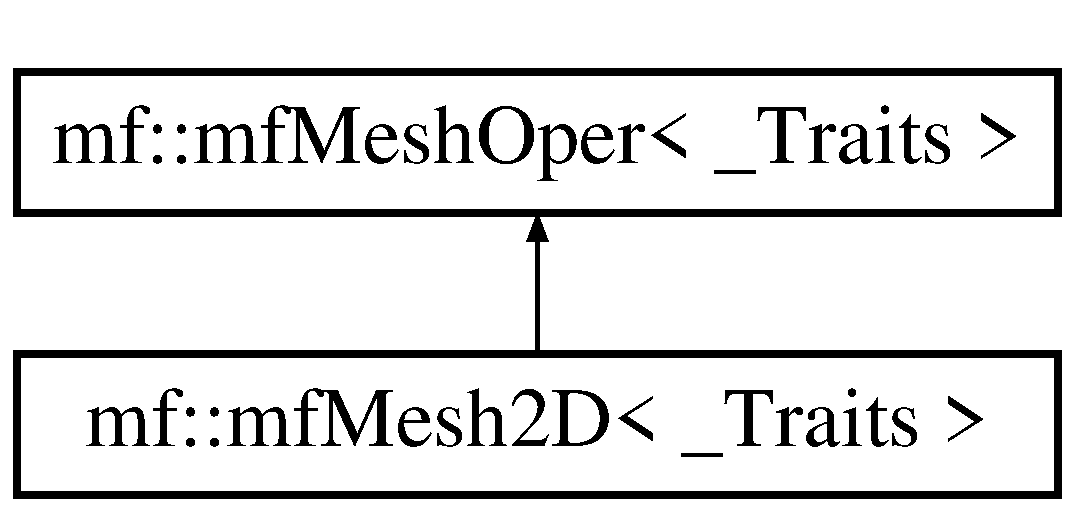
\includegraphics[height=2.000000cm]{classmf_1_1mfMesh2D}
\end{center}
\end{figure}
\subsection*{Public Types}
\begin{DoxyCompactItemize}
\item 
typedef \_\-Traits::ids \hyperlink{classmf_1_1mfMesh2D_a517d508b5d1959b3c697f7c393ccd068}{ids}
\item 
\hypertarget{classmf_1_1mfMesh2D_ae76d2188c161d108b11b434253ac708a}{
typedef \_\-Traits::sVertex {\bfseries sVertex}}
\label{classmf_1_1mfMesh2D_ae76d2188c161d108b11b434253ac708a}

\item 
\hypertarget{classmf_1_1mfMesh2D_ad98ffaf6cec43224918e35b7272a5168}{
typedef \_\-Traits::sCell {\bfseries sCell}}
\label{classmf_1_1mfMesh2D_ad98ffaf6cec43224918e35b7272a5168}

\item 
\hypertarget{classmf_1_1mfMesh2D_a6bfcc84cc5bd3a12e15c8255c2e36b6b}{
typedef \_\-Traits::sGeometric {\bfseries sGeometric}}
\label{classmf_1_1mfMesh2D_a6bfcc84cc5bd3a12e15c8255c2e36b6b}

\item 
\hypertarget{classmf_1_1mfMesh2D_a360cbe8e1a25a9fb4234e3028be77fe6}{
typedef \_\-Traits::sTopology {\bfseries sTopology}}
\label{classmf_1_1mfMesh2D_a360cbe8e1a25a9fb4234e3028be77fe6}

\item 
\hypertarget{classmf_1_1mfMesh2D_adcf3197707a7cdd4a121b080b97c1ce1}{
typedef \hyperlink{classmf_1_1mfSing}{mfSing}$<$ \_\-Traits $>$ {\bfseries sSing}}
\label{classmf_1_1mfMesh2D_adcf3197707a7cdd4a121b080b97c1ce1}

\item 
typedef \_\-Traits::sMesh \hyperlink{classmf_1_1mfMesh2D_aa197f7f92e5aa8e68703a5eeb3d9ae04}{sMesh}
\end{DoxyCompactItemize}
\subsection*{Public Member Functions}
\begin{DoxyCompactItemize}
\item 
\hyperlink{classmf_1_1mfMesh2D_a5cea95cc70113a2d0c3fcd2361386cc7}{mfMesh2D} (\hyperlink{classmf_1_1mfMesh2D_aa197f7f92e5aa8e68703a5eeb3d9ae04}{sMesh} $\ast$\_\-mesh)
\item 
\hyperlink{classmf_1_1mfMesh2D_a7758ae67057192a0f348a09b1f020a63}{$\sim$mfMesh2D} ()
\item 
void \hyperlink{classmf_1_1mfMesh2D_a03936ceb5649223ff6dc548cf22b4cf7}{addCell} (\hyperlink{classmf_1_1mfMesh2D_a517d508b5d1959b3c697f7c393ccd068}{ids} idcell, \hyperlink{classmf_1_1mfMesh2D_a517d508b5d1959b3c697f7c393ccd068}{ids} $\ast$idvertices MF\_\-DMUTEXVD)
\item 
\hypertarget{classmf_1_1mfMesh2D_aff5a924abb5bcce8be4595aa4a3b6137}{
void {\bfseries addCell} (\hyperlink{classmf_1_1mfMesh2D_a517d508b5d1959b3c697f7c393ccd068}{ids} idcell, \hyperlink{classmf_1_1mfMesh2D_a517d508b5d1959b3c697f7c393ccd068}{ids} $\ast$idvertices, \hyperlink{classmf_1_1mfMesh2D_a517d508b5d1959b3c697f7c393ccd068}{ids} $\ast$idops MF\_\-DMUTEXVD)}
\label{classmf_1_1mfMesh2D_aff5a924abb5bcce8be4595aa4a3b6137}

\item 
void \hyperlink{classmf_1_1mfMesh2D_ada59f56b773f4951e2db41826ab8b644}{delCell} (\hyperlink{classmf_1_1mfMesh2D_a517d508b5d1959b3c697f7c393ccd068}{ids} idcell MF\_\-DMUTEXVD)
\end{DoxyCompactItemize}


\subsection{Detailed Description}
\subsubsection*{template$<$class \_\-Traits$>$ class mf::mfMesh2D$<$ \_\-Traits $>$}

Operation Class for Triangles in 2D space

\_\-Traits must have: ids, sVertex, sCell, sSing, sMesh, sGeometric 

\subsection{Member Typedef Documentation}
\hypertarget{classmf_1_1mfMesh2D_a517d508b5d1959b3c697f7c393ccd068}{
\index{mf::mfMesh2D@{mf::mfMesh2D}!ids@{ids}}
\index{ids@{ids}!mf::mfMesh2D@{mf::mfMesh2D}}
\subsubsection[{ids}]{\setlength{\rightskip}{0pt plus 5cm}template$<$class \_\-Traits $>$ typedef \_\-Traits::ids {\bf mf::mfMesh2D}$<$ \_\-Traits $>$::{\bf ids}}}
\label{classmf_1_1mfMesh2D_a517d508b5d1959b3c697f7c393ccd068}
Id typename definition 

Reimplemented from \hyperlink{classmf_1_1mfMeshOper_a526d1466339244781fbdc0dbfe5ad210}{mf::mfMeshOper$<$ \_\-Traits $>$}.

\hypertarget{classmf_1_1mfMesh2D_aa197f7f92e5aa8e68703a5eeb3d9ae04}{
\index{mf::mfMesh2D@{mf::mfMesh2D}!sMesh@{sMesh}}
\index{sMesh@{sMesh}!mf::mfMesh2D@{mf::mfMesh2D}}
\subsubsection[{sMesh}]{\setlength{\rightskip}{0pt plus 5cm}template$<$class \_\-Traits $>$ typedef \_\-Traits::sMesh {\bf mf::mfMesh2D}$<$ \_\-Traits $>$::{\bf sMesh}}}
\label{classmf_1_1mfMesh2D_aa197f7f92e5aa8e68703a5eeb3d9ae04}
Mesh typename definition 

Reimplemented from \hyperlink{classmf_1_1mfMeshOper_a96c05da9a054cf9ac58d15211922f936}{mf::mfMeshOper$<$ \_\-Traits $>$}.



\subsection{Constructor \& Destructor Documentation}
\hypertarget{classmf_1_1mfMesh2D_a5cea95cc70113a2d0c3fcd2361386cc7}{
\index{mf::mfMesh2D@{mf::mfMesh2D}!mfMesh2D@{mfMesh2D}}
\index{mfMesh2D@{mfMesh2D}!mf::mfMesh2D@{mf::mfMesh2D}}
\subsubsection[{mfMesh2D}]{\setlength{\rightskip}{0pt plus 5cm}template$<$class \_\-Traits $>$ {\bf mf::mfMesh2D}$<$ \_\-Traits $>$::{\bf mfMesh2D} (
\begin{DoxyParamCaption}
\item[{{\bf sMesh} $\ast$}]{\_\-mesh}
\end{DoxyParamCaption}
)}}
\label{classmf_1_1mfMesh2D_a5cea95cc70113a2d0c3fcd2361386cc7}
Constructor


\begin{DoxyParams}{Parameters}
{\em \_\-mesh,:} & the mesh address that this class will manipulate \\
\hline
\end{DoxyParams}
\hypertarget{classmf_1_1mfMesh2D_a7758ae67057192a0f348a09b1f020a63}{
\index{mf::mfMesh2D@{mf::mfMesh2D}!$\sim$mfMesh2D@{$\sim$mfMesh2D}}
\index{$\sim$mfMesh2D@{$\sim$mfMesh2D}!mf::mfMesh2D@{mf::mfMesh2D}}
\subsubsection[{$\sim$mfMesh2D}]{\setlength{\rightskip}{0pt plus 5cm}template$<$class \_\-Traits $>$ {\bf mf::mfMesh2D}$<$ \_\-Traits $>$::$\sim${\bf mfMesh2D} (
\begin{DoxyParamCaption}
{}
\end{DoxyParamCaption}
)}}
\label{classmf_1_1mfMesh2D_a7758ae67057192a0f348a09b1f020a63}
Destructor 

\subsection{Member Function Documentation}
\hypertarget{classmf_1_1mfMesh2D_a03936ceb5649223ff6dc548cf22b4cf7}{
\index{mf::mfMesh2D@{mf::mfMesh2D}!addCell@{addCell}}
\index{addCell@{addCell}!mf::mfMesh2D@{mf::mfMesh2D}}
\subsubsection[{addCell}]{\setlength{\rightskip}{0pt plus 5cm}template$<$class \_\-Traits $>$ void {\bf mf::mfMesh2D}$<$ \_\-Traits $>$::addCell (
\begin{DoxyParamCaption}
\item[{{\bf ids}}]{idcell, }
\item[{{\bf ids} $\ast$idvertices}]{MF\_\-DMUTEXVD}
\end{DoxyParamCaption}
)}}
\label{classmf_1_1mfMesh2D_a03936ceb5649223ff6dc548cf22b4cf7}
Add cell in mesh


\begin{DoxyParams}{Parameters}
{\em idcell,:} & cell id \\
\hline
{\em idvertices,:} & vector with vertices ids of the cell \\
\hline
\end{DoxyParams}
\hypertarget{classmf_1_1mfMesh2D_ada59f56b773f4951e2db41826ab8b644}{
\index{mf::mfMesh2D@{mf::mfMesh2D}!delCell@{delCell}}
\index{delCell@{delCell}!mf::mfMesh2D@{mf::mfMesh2D}}
\subsubsection[{delCell}]{\setlength{\rightskip}{0pt plus 5cm}template$<$class \_\-Traits $>$ void {\bf mf::mfMesh2D}$<$ \_\-Traits $>$::delCell (
\begin{DoxyParamCaption}
\item[{{\bf ids} idcell}]{MF\_\-DMUTEXVD}
\end{DoxyParamCaption}
)}}
\label{classmf_1_1mfMesh2D_ada59f56b773f4951e2db41826ab8b644}
Delete a cell


\begin{DoxyParams}{Parameters}
{\em idcell,:} & cell id \\
\hline
\end{DoxyParams}


The documentation for this class was generated from the following file:\begin{DoxyCompactItemize}
\item 
mfMesh2D.h\end{DoxyCompactItemize}

\hypertarget{classmf_1_1mfMesh3D}{
\section{mf::mfMesh3D$<$ \_\-Traits $>$ Class Template Reference}
\label{classmf_1_1mfMesh3D}\index{mf::mfMesh3D@{mf::mfMesh3D}}
}
\subsection*{Public Types}
\begin{DoxyCompactItemize}
\item 
typedef \_\-Traits::space \hyperlink{classmf_1_1mfMesh3D_aea7155b49fb50982a399056973e6b4d8}{space}
\item 
typedef \_\-Traits::ids \hyperlink{classmf_1_1mfMesh3D_aeae559d0564bf64617c8fd83ba264895}{ids}
\item 
typedef \_\-Traits::sVertex \hyperlink{classmf_1_1mfMesh3D_ac523ee47bc707949d351f9f73d09677e}{sVertex}
\item 
typedef \_\-Traits::sCell \hyperlink{classmf_1_1mfMesh3D_acbb717ca80998e53d622ab2ae35b9134}{sCell}
\item 
typedef \_\-Traits::sEdge \hyperlink{classmf_1_1mfMesh3D_a93992ed7712bd9dbcc0430166a540d1c}{sEdge}
\item 
typedef \_\-Traits::sEdge \hyperlink{classmf_1_1mfMesh3D_ae70500195d62c66dc79d18394652a2af}{sFace}
\item 
typedef \_\-Traits::sOper \hyperlink{classmf_1_1mfMesh3D_ab30b285a3a7387627cf13798561050a0}{sOper}
\item 
typedef \_\-Traits::sTopology \hyperlink{classmf_1_1mfMesh3D_af51322fa414c9ddd714ef2088651a794}{sTopology}
\end{DoxyCompactItemize}
\subsection*{Public Member Functions}
\begin{DoxyCompactItemize}
\item 
\hyperlink{classmf_1_1mfMesh3D_a91b5fd82f7f202d9b01519e4baad3f93}{mfMesh3D} (\hyperlink{classmf_1_1mfMesh3D_aeae559d0564bf64617c8fd83ba264895}{ids} block\_\-size=5000)
\item 
\hyperlink{classmf_1_1mfMesh3D_af54049813d1e1050fc123fcbca6b10c1}{$\sim$mfMesh3D} ()
\item 
\hyperlink{classmf_1_1mfMesh3D_aeae559d0564bf64617c8fd83ba264895}{ids} \hyperlink{classmf_1_1mfMesh3D_acd7ae4e46082dc88ff6a2ec0e3833997}{addVertex} (\hyperlink{classmf_1_1mfMesh3D_aea7155b49fb50982a399056973e6b4d8}{space} $\ast$coords MF\_\-DMUTEXVD)
\item 
bool \hyperlink{classmf_1_1mfMesh3D_a6cef73e9208a423066e439f30c852a0a}{delVertex} (\hyperlink{classmf_1_1mfMesh3D_aeae559d0564bf64617c8fd83ba264895}{ids} idvertex MF\_\-DMUTEXVD)
\item 
\hyperlink{classmf_1_1mfMesh3D_aeae559d0564bf64617c8fd83ba264895}{ids} \hyperlink{classmf_1_1mfMesh3D_a542735e173f7c4937bd9fd6ae9dae715}{getNumberOfVertices} (MF\_\-DMUTEXD)
\item 
\hyperlink{classmf_1_1mfMesh3D_aeae559d0564bf64617c8fd83ba264895}{ids} \hyperlink{classmf_1_1mfMesh3D_a3ad267a7abdfec7e511c93031b6304a3}{getVertexMaxId} (MF\_\-DMUTEXD)
\item 
\hyperlink{classmf_1_1mfMesh3D_ac523ee47bc707949d351f9f73d09677e}{sVertex} $\ast$ \hyperlink{classmf_1_1mfMesh3D_ab3b20eb8024e905f22dca14b139ec1a8}{getVertex} (\hyperlink{classmf_1_1mfMesh3D_aeae559d0564bf64617c8fd83ba264895}{ids} idvertex MF\_\-DMUTEXVD)
\item 
bool \hyperlink{classmf_1_1mfMesh3D_afec11a472590da7e8f7740a0bddce106}{isVertex} (\hyperlink{classmf_1_1mfMesh3D_aeae559d0564bf64617c8fd83ba264895}{ids} idvertex MF\_\-DMUTEXVD)
\item 
\hyperlink{classmf_1_1mfMesh3D_aeae559d0564bf64617c8fd83ba264895}{ids} \hyperlink{classmf_1_1mfMesh3D_a237521684246bd6c5171e72aa95cdf2b}{addCell} (\hyperlink{classmf_1_1mfMesh3D_aeae559d0564bf64617c8fd83ba264895}{ids} $\ast$idvertices MF\_\-DMUTEXVD)
\item 
bool \hyperlink{classmf_1_1mfMesh3D_a75f082e8b945188ab1996193a527b143}{delCell} (\hyperlink{classmf_1_1mfMesh3D_aeae559d0564bf64617c8fd83ba264895}{ids} idcell MF\_\-DMUTEXVD)
\item 
\hyperlink{classmf_1_1mfMesh3D_aeae559d0564bf64617c8fd83ba264895}{ids} \hyperlink{classmf_1_1mfMesh3D_a7a5fb0879d87329788fee8ffdfd64932}{getNumberOfCells} (MF\_\-DMUTEXD)
\item 
\hyperlink{classmf_1_1mfMesh3D_aeae559d0564bf64617c8fd83ba264895}{ids} \hyperlink{classmf_1_1mfMesh3D_a73c24174352c1b169b9b82a8dd51a01c}{getCellMaxId} (MF\_\-DMUTEXD)
\item 
\hyperlink{classmf_1_1mfMesh3D_acbb717ca80998e53d622ab2ae35b9134}{sCell} $\ast$ \hyperlink{classmf_1_1mfMesh3D_aaad815afdc1d7e0e49cd4e904db6cc93}{getCell} (\hyperlink{classmf_1_1mfMesh3D_aeae559d0564bf64617c8fd83ba264895}{ids} idcell MF\_\-DMUTEXVD)
\item 
bool \hyperlink{classmf_1_1mfMesh3D_a578c15c12e4d351e61b4d88b6d844049}{isCell} (\hyperlink{classmf_1_1mfMesh3D_aeae559d0564bf64617c8fd83ba264895}{ids} idcell MF\_\-DMUTEXVD)
\item 
void \hyperlink{classmf_1_1mfMesh3D_a5db400ff5cacf7832427b58f2b5c10a5}{setNumberOfVertices} (\hyperlink{classmf_1_1mfMesh3D_aeae559d0564bf64617c8fd83ba264895}{ids} number MF\_\-DMUTEXVD)
\item 
void \hyperlink{classmf_1_1mfMesh3D_a4d70787f5afc60ec09d0ede007cc92c4}{setNumberOfCells} (\hyperlink{classmf_1_1mfMesh3D_aeae559d0564bf64617c8fd83ba264895}{ids} number MF\_\-DMUTEXVD)
\item 
void \hyperlink{classmf_1_1mfMesh3D_a5db5e246c9c63b3988e1606f03bf8715}{addVertex} (\hyperlink{classmf_1_1mfMesh3D_aeae559d0564bf64617c8fd83ba264895}{ids} idvertex, \hyperlink{classmf_1_1mfMesh3D_aea7155b49fb50982a399056973e6b4d8}{space} $\ast$coords MF\_\-DMUTEXVD)
\item 
void \hyperlink{classmf_1_1mfMesh3D_a399b9e8291ea7bc29fa09faaed72db61}{addCell} (\hyperlink{classmf_1_1mfMesh3D_aeae559d0564bf64617c8fd83ba264895}{ids} idcell, \hyperlink{classmf_1_1mfMesh3D_aeae559d0564bf64617c8fd83ba264895}{ids} $\ast$idvertices MF\_\-DMUTEXVD)
\item 
\hypertarget{classmf_1_1mfMesh3D_a7e80d96081ccab4af16ddf3c3a76071e}{
\hyperlink{classmf_1_1mfMesh3D_aeae559d0564bf64617c8fd83ba264895}{ids} {\bfseries addCell} (\hyperlink{classmf_1_1mfMesh3D_aeae559d0564bf64617c8fd83ba264895}{ids} $\ast$idvertices, \hyperlink{classmf_1_1mfMesh3D_aeae559d0564bf64617c8fd83ba264895}{ids} $\ast$idops MF\_\-DMUTEXVD)}
\label{classmf_1_1mfMesh3D_a7e80d96081ccab4af16ddf3c3a76071e}

\item 
\hyperlink{classmf_1_1mfMesh3D_aeae559d0564bf64617c8fd83ba264895}{ids} \hyperlink{classmf_1_1mfMesh3D_a10ce55cc76de42b5aa0f7c4244763f44}{addEdge} ()
\item 
\hyperlink{classmf_1_1mfMesh3D_aeae559d0564bf64617c8fd83ba264895}{ids} \hyperlink{classmf_1_1mfMesh3D_adaf8348280fa19542ea5de9ba47f1d12}{getNumberOfEdges} (MF\_\-DMUTEXD)
\item 
\hyperlink{classmf_1_1mfMesh3D_aeae559d0564bf64617c8fd83ba264895}{ids} \hyperlink{classmf_1_1mfMesh3D_a2dd4c8a343fa1173b6a7c78b4aa050b0}{getEdgeMaxId} (MF\_\-DMUTEXD)
\item 
\hyperlink{classmf_1_1mfMesh3D_a93992ed7712bd9dbcc0430166a540d1c}{sEdge} $\ast$ \hyperlink{classmf_1_1mfMesh3D_a7a033f10bb1bc509d62a53f34086e220}{getEdge} (\hyperlink{classmf_1_1mfMesh3D_aeae559d0564bf64617c8fd83ba264895}{ids} idEdge MF\_\-DMUTEXVD)
\item 
bool \hyperlink{classmf_1_1mfMesh3D_a63b15118d28b6f6ceb4b19670148788a}{isEdge} (\hyperlink{classmf_1_1mfMesh3D_aeae559d0564bf64617c8fd83ba264895}{ids} idEdgex MF\_\-DMUTEXVD)
\item 
\hypertarget{classmf_1_1mfMesh3D_a4bba26cee832afb1474ae9e8f6549525}{
\hyperlink{classmf_1_1mfMesh3D_aeae559d0564bf64617c8fd83ba264895}{ids} {\bfseries getBlockSize} ()}
\label{classmf_1_1mfMesh3D_a4bba26cee832afb1474ae9e8f6549525}

\item 
\hypertarget{classmf_1_1mfMesh3D_a5c1dd2261484b87e16fddbe0e276a977}{
void {\bfseries freeCell} (\hyperlink{classmf_1_1mfMesh3D_aeae559d0564bf64617c8fd83ba264895}{ids} idcell MF\_\-DMUTEXVD)}
\label{classmf_1_1mfMesh3D_a5c1dd2261484b87e16fddbe0e276a977}

\item 
\hypertarget{classmf_1_1mfMesh3D_a859fade6e91a75968a66e72aa33f6a4a}{
void {\bfseries freeVertex} (\hyperlink{classmf_1_1mfMesh3D_aeae559d0564bf64617c8fd83ba264895}{ids} idvertex MF\_\-DMUTEXVD)}
\label{classmf_1_1mfMesh3D_a859fade6e91a75968a66e72aa33f6a4a}

\item 
\hypertarget{classmf_1_1mfMesh3D_a437b244a6f61a1f0d225cff9c739b064}{
void {\bfseries freeEdge} (\hyperlink{classmf_1_1mfMesh3D_aeae559d0564bf64617c8fd83ba264895}{ids} idedge MF\_\-DMUTEXVD)}
\label{classmf_1_1mfMesh3D_a437b244a6f61a1f0d225cff9c739b064}

\end{DoxyCompactItemize}
\subsubsection*{template$<$class \_\-Traits$>$ class mf::mfMesh3D$<$ \_\-Traits $>$}



\subsection{Member Typedef Documentation}
\hypertarget{classmf_1_1mfMesh3D_aeae559d0564bf64617c8fd83ba264895}{
\index{mf::mfMesh3D@{mf::mfMesh3D}!ids@{ids}}
\index{ids@{ids}!mf::mfMesh3D@{mf::mfMesh3D}}
\subsubsection[{ids}]{\setlength{\rightskip}{0pt plus 5cm}template$<$class \_\-Traits $>$ typedef \_\-Traits::ids {\bf mf::mfMesh3D}$<$ \_\-Traits $>$::{\bf ids}}}
\label{classmf_1_1mfMesh3D_aeae559d0564bf64617c8fd83ba264895}
Id typename definition \hypertarget{classmf_1_1mfMesh3D_acbb717ca80998e53d622ab2ae35b9134}{
\index{mf::mfMesh3D@{mf::mfMesh3D}!sCell@{sCell}}
\index{sCell@{sCell}!mf::mfMesh3D@{mf::mfMesh3D}}
\subsubsection[{sCell}]{\setlength{\rightskip}{0pt plus 5cm}template$<$class \_\-Traits $>$ typedef \_\-Traits::sCell {\bf mf::mfMesh3D}$<$ \_\-Traits $>$::{\bf sCell}}}
\label{classmf_1_1mfMesh3D_acbb717ca80998e53d622ab2ae35b9134}
Cell typename definition \hypertarget{classmf_1_1mfMesh3D_a93992ed7712bd9dbcc0430166a540d1c}{
\index{mf::mfMesh3D@{mf::mfMesh3D}!sEdge@{sEdge}}
\index{sEdge@{sEdge}!mf::mfMesh3D@{mf::mfMesh3D}}
\subsubsection[{sEdge}]{\setlength{\rightskip}{0pt plus 5cm}template$<$class \_\-Traits $>$ typedef \_\-Traits::sEdge {\bf mf::mfMesh3D}$<$ \_\-Traits $>$::{\bf sEdge}}}
\label{classmf_1_1mfMesh3D_a93992ed7712bd9dbcc0430166a540d1c}
Edge typename definition \hypertarget{classmf_1_1mfMesh3D_ae70500195d62c66dc79d18394652a2af}{
\index{mf::mfMesh3D@{mf::mfMesh3D}!sFace@{sFace}}
\index{sFace@{sFace}!mf::mfMesh3D@{mf::mfMesh3D}}
\subsubsection[{sFace}]{\setlength{\rightskip}{0pt plus 5cm}template$<$class \_\-Traits $>$ typedef \_\-Traits::sEdge {\bf mf::mfMesh3D}$<$ \_\-Traits $>$::{\bf sFace}}}
\label{classmf_1_1mfMesh3D_ae70500195d62c66dc79d18394652a2af}
Edge typename definition \hypertarget{classmf_1_1mfMesh3D_ab30b285a3a7387627cf13798561050a0}{
\index{mf::mfMesh3D@{mf::mfMesh3D}!sOper@{sOper}}
\index{sOper@{sOper}!mf::mfMesh3D@{mf::mfMesh3D}}
\subsubsection[{sOper}]{\setlength{\rightskip}{0pt plus 5cm}template$<$class \_\-Traits $>$ typedef \_\-Traits::sOper {\bf mf::mfMesh3D}$<$ \_\-Traits $>$::{\bf sOper}}}
\label{classmf_1_1mfMesh3D_ab30b285a3a7387627cf13798561050a0}
Operator typename definition \hypertarget{classmf_1_1mfMesh3D_aea7155b49fb50982a399056973e6b4d8}{
\index{mf::mfMesh3D@{mf::mfMesh3D}!space@{space}}
\index{space@{space}!mf::mfMesh3D@{mf::mfMesh3D}}
\subsubsection[{space}]{\setlength{\rightskip}{0pt plus 5cm}template$<$class \_\-Traits $>$ typedef \_\-Traits::space {\bf mf::mfMesh3D}$<$ \_\-Traits $>$::{\bf space}}}
\label{classmf_1_1mfMesh3D_aea7155b49fb50982a399056973e6b4d8}
Space typename definition \hypertarget{classmf_1_1mfMesh3D_af51322fa414c9ddd714ef2088651a794}{
\index{mf::mfMesh3D@{mf::mfMesh3D}!sTopology@{sTopology}}
\index{sTopology@{sTopology}!mf::mfMesh3D@{mf::mfMesh3D}}
\subsubsection[{sTopology}]{\setlength{\rightskip}{0pt plus 5cm}template$<$class \_\-Traits $>$ typedef \_\-Traits::sTopology {\bf mf::mfMesh3D}$<$ \_\-Traits $>$::{\bf sTopology}}}
\label{classmf_1_1mfMesh3D_af51322fa414c9ddd714ef2088651a794}
Topology typename definition \hypertarget{classmf_1_1mfMesh3D_ac523ee47bc707949d351f9f73d09677e}{
\index{mf::mfMesh3D@{mf::mfMesh3D}!sVertex@{sVertex}}
\index{sVertex@{sVertex}!mf::mfMesh3D@{mf::mfMesh3D}}
\subsubsection[{sVertex}]{\setlength{\rightskip}{0pt plus 5cm}template$<$class \_\-Traits $>$ typedef \_\-Traits::sVertex {\bf mf::mfMesh3D}$<$ \_\-Traits $>$::{\bf sVertex}}}
\label{classmf_1_1mfMesh3D_ac523ee47bc707949d351f9f73d09677e}
Vertex typename definition 

\subsection{Constructor \& Destructor Documentation}
\hypertarget{classmf_1_1mfMesh3D_a91b5fd82f7f202d9b01519e4baad3f93}{
\index{mf::mfMesh3D@{mf::mfMesh3D}!mfMesh3D@{mfMesh3D}}
\index{mfMesh3D@{mfMesh3D}!mf::mfMesh3D@{mf::mfMesh3D}}
\subsubsection[{mfMesh3D}]{\setlength{\rightskip}{0pt plus 5cm}template$<$class \_\-Traits $>$ {\bf mf::mfMesh3D}$<$ \_\-Traits $>$::{\bf mfMesh3D} (
\begin{DoxyParamCaption}
\item[{{\bf ids}}]{block\_\-size = {\ttfamily 5000}}
\end{DoxyParamCaption}
)}}
\label{classmf_1_1mfMesh3D_a91b5fd82f7f202d9b01519e4baad3f93}
Constructor


\begin{DoxyParams}{Parameters}
{\em block\_\-size,:} & size of vector blocks. The maximum size of vector is block\_\-size $\ast$ block\_\-size \\
\hline
\end{DoxyParams}
\hypertarget{classmf_1_1mfMesh3D_af54049813d1e1050fc123fcbca6b10c1}{
\index{mf::mfMesh3D@{mf::mfMesh3D}!$\sim$mfMesh3D@{$\sim$mfMesh3D}}
\index{$\sim$mfMesh3D@{$\sim$mfMesh3D}!mf::mfMesh3D@{mf::mfMesh3D}}
\subsubsection[{$\sim$mfMesh3D}]{\setlength{\rightskip}{0pt plus 5cm}template$<$class \_\-Traits $>$ {\bf mf::mfMesh3D}$<$ \_\-Traits $>$::$\sim${\bf mfMesh3D} (
\begin{DoxyParamCaption}
{}
\end{DoxyParamCaption}
)}}
\label{classmf_1_1mfMesh3D_af54049813d1e1050fc123fcbca6b10c1}
Destructor 

\subsection{Member Function Documentation}
\hypertarget{classmf_1_1mfMesh3D_a237521684246bd6c5171e72aa95cdf2b}{
\index{mf::mfMesh3D@{mf::mfMesh3D}!addCell@{addCell}}
\index{addCell@{addCell}!mf::mfMesh3D@{mf::mfMesh3D}}
\subsubsection[{addCell}]{\setlength{\rightskip}{0pt plus 5cm}template$<$class \_\-Traits $>$ IDS {\bf mf::mfMesh3D}$<$ \_\-Traits $>$::addCell (
\begin{DoxyParamCaption}
\item[{{\bf ids} $\ast$idvertices}]{MF\_\-DMUTEXVD}
\end{DoxyParamCaption}
)}}
\label{classmf_1_1mfMesh3D_a237521684246bd6c5171e72aa95cdf2b}
Add a cell in mesh


\begin{DoxyParams}{Parameters}
{\em idvertices,:} & vector with vertices ids of the cell\\
\hline
\end{DoxyParams}
\begin{DoxyReturn}{Returns}
the cell id in mesh 
\end{DoxyReturn}
\hypertarget{classmf_1_1mfMesh3D_a399b9e8291ea7bc29fa09faaed72db61}{
\index{mf::mfMesh3D@{mf::mfMesh3D}!addCell@{addCell}}
\index{addCell@{addCell}!mf::mfMesh3D@{mf::mfMesh3D}}
\subsubsection[{addCell}]{\setlength{\rightskip}{0pt plus 5cm}template$<$class \_\-Traits $>$ void {\bf mf::mfMesh3D}$<$ \_\-Traits $>$::addCell (
\begin{DoxyParamCaption}
\item[{{\bf ids}}]{idcell, }
\item[{{\bf ids} $\ast$idvertices}]{MF\_\-DMUTEXVD}
\end{DoxyParamCaption}
)}}
\label{classmf_1_1mfMesh3D_a399b9e8291ea7bc29fa09faaed72db61}
Add a cell in specified position in mesh


\begin{DoxyParams}{Parameters}
{\em idvertex,:} & position of cell \\
\hline
{\em idvertices,:} & vector with vertices ids of the cell\\
\hline
\end{DoxyParams}
\begin{DoxyReturn}{Returns}
the cell id in mesh 
\end{DoxyReturn}
\hypertarget{classmf_1_1mfMesh3D_a10ce55cc76de42b5aa0f7c4244763f44}{
\index{mf::mfMesh3D@{mf::mfMesh3D}!addEdge@{addEdge}}
\index{addEdge@{addEdge}!mf::mfMesh3D@{mf::mfMesh3D}}
\subsubsection[{addEdge}]{\setlength{\rightskip}{0pt plus 5cm}template$<$class \_\-Traits $>$ IDS {\bf mf::mfMesh3D}$<$ \_\-Traits $>$::addEdge (
\begin{DoxyParamCaption}
{}
\end{DoxyParamCaption}
)}}
\label{classmf_1_1mfMesh3D_a10ce55cc76de42b5aa0f7c4244763f44}
Add a edge in mesh

\begin{DoxyReturn}{Returns}
the edge id in mesh 
\end{DoxyReturn}
\hypertarget{classmf_1_1mfMesh3D_acd7ae4e46082dc88ff6a2ec0e3833997}{
\index{mf::mfMesh3D@{mf::mfMesh3D}!addVertex@{addVertex}}
\index{addVertex@{addVertex}!mf::mfMesh3D@{mf::mfMesh3D}}
\subsubsection[{addVertex}]{\setlength{\rightskip}{0pt plus 5cm}template$<$class \_\-Traits $>$ IDS {\bf mf::mfMesh3D}$<$ \_\-Traits $>$::addVertex (
\begin{DoxyParamCaption}
\item[{{\bf space} $\ast$coords}]{MF\_\-DMUTEXVD}
\end{DoxyParamCaption}
)}}
\label{classmf_1_1mfMesh3D_acd7ae4e46082dc88ff6a2ec0e3833997}
Add a vertex in mesh


\begin{DoxyParams}{Parameters}
{\em coords,:} & vector with the vertex coordinates\\
\hline
\end{DoxyParams}
\begin{DoxyReturn}{Returns}
the vertex id in mesh 
\end{DoxyReturn}
\hypertarget{classmf_1_1mfMesh3D_a5db5e246c9c63b3988e1606f03bf8715}{
\index{mf::mfMesh3D@{mf::mfMesh3D}!addVertex@{addVertex}}
\index{addVertex@{addVertex}!mf::mfMesh3D@{mf::mfMesh3D}}
\subsubsection[{addVertex}]{\setlength{\rightskip}{0pt plus 5cm}template$<$class \_\-Traits $>$ void {\bf mf::mfMesh3D}$<$ \_\-Traits $>$::addVertex (
\begin{DoxyParamCaption}
\item[{{\bf ids}}]{idvertex, }
\item[{{\bf space} $\ast$coords}]{MF\_\-DMUTEXVD}
\end{DoxyParamCaption}
)}}
\label{classmf_1_1mfMesh3D_a5db5e246c9c63b3988e1606f03bf8715}
Add a vertex in specified position in mesh


\begin{DoxyParams}{Parameters}
{\em idvertex,:} & position of vertex \\
\hline
{\em coords,:} & vector with the vertex coordinates\\
\hline
\end{DoxyParams}
\begin{DoxyReturn}{Returns}
the vertex id in mesh 
\end{DoxyReturn}
\hypertarget{classmf_1_1mfMesh3D_a75f082e8b945188ab1996193a527b143}{
\index{mf::mfMesh3D@{mf::mfMesh3D}!delCell@{delCell}}
\index{delCell@{delCell}!mf::mfMesh3D@{mf::mfMesh3D}}
\subsubsection[{delCell}]{\setlength{\rightskip}{0pt plus 5cm}template$<$class \_\-Traits $>$ bool {\bf mf::mfMesh3D}$<$ \_\-Traits $>$::delCell (
\begin{DoxyParamCaption}
\item[{{\bf ids} idcell}]{MF\_\-DMUTEXVD}
\end{DoxyParamCaption}
)}}
\label{classmf_1_1mfMesh3D_a75f082e8b945188ab1996193a527b143}
Delete a cell in mesh


\begin{DoxyParams}{Parameters}
{\em idcell,:} & the cell is\\
\hline
\end{DoxyParams}
\begin{DoxyReturn}{Returns}
true if the cell was deleted 
\end{DoxyReturn}
\hypertarget{classmf_1_1mfMesh3D_a6cef73e9208a423066e439f30c852a0a}{
\index{mf::mfMesh3D@{mf::mfMesh3D}!delVertex@{delVertex}}
\index{delVertex@{delVertex}!mf::mfMesh3D@{mf::mfMesh3D}}
\subsubsection[{delVertex}]{\setlength{\rightskip}{0pt plus 5cm}template$<$class \_\-Traits $>$ bool {\bf mf::mfMesh3D}$<$ \_\-Traits $>$::delVertex (
\begin{DoxyParamCaption}
\item[{{\bf ids} idvertex}]{MF\_\-DMUTEXVD}
\end{DoxyParamCaption}
)}}
\label{classmf_1_1mfMesh3D_a6cef73e9208a423066e439f30c852a0a}
Delete a vertex in mesh


\begin{DoxyParams}{Parameters}
{\em idvertex,:} & the vertex will be deleted\\
\hline
\end{DoxyParams}
\begin{DoxyReturn}{Returns}
true if the vertex was deleted 
\end{DoxyReturn}
\hypertarget{classmf_1_1mfMesh3D_aaad815afdc1d7e0e49cd4e904db6cc93}{
\index{mf::mfMesh3D@{mf::mfMesh3D}!getCell@{getCell}}
\index{getCell@{getCell}!mf::mfMesh3D@{mf::mfMesh3D}}
\subsubsection[{getCell}]{\setlength{\rightskip}{0pt plus 5cm}template$<$class \_\-Traits $>$ SCELL $\ast$ {\bf mf::mfMesh3D}$<$ \_\-Traits $>$::getCell (
\begin{DoxyParamCaption}
\item[{{\bf ids} idcell}]{MF\_\-DMUTEXVD}
\end{DoxyParamCaption}
)}}
\label{classmf_1_1mfMesh3D_aaad815afdc1d7e0e49cd4e904db6cc93}
Return the cell address


\begin{DoxyParams}{Parameters}
{\em idcell,:} & the cell id \\
\hline
\end{DoxyParams}
\hypertarget{classmf_1_1mfMesh3D_a73c24174352c1b169b9b82a8dd51a01c}{
\index{mf::mfMesh3D@{mf::mfMesh3D}!getCellMaxId@{getCellMaxId}}
\index{getCellMaxId@{getCellMaxId}!mf::mfMesh3D@{mf::mfMesh3D}}
\subsubsection[{getCellMaxId}]{\setlength{\rightskip}{0pt plus 5cm}template$<$class \_\-Traits $>$ IDS {\bf mf::mfMesh3D}$<$ \_\-Traits $>$::getCellMaxId (
\begin{DoxyParamCaption}
\item[{MF\_\-DMUTEXD}]{}
\end{DoxyParamCaption}
)}}
\label{classmf_1_1mfMesh3D_a73c24174352c1b169b9b82a8dd51a01c}
Return the greater cell id in mesh \hypertarget{classmf_1_1mfMesh3D_a7a033f10bb1bc509d62a53f34086e220}{
\index{mf::mfMesh3D@{mf::mfMesh3D}!getEdge@{getEdge}}
\index{getEdge@{getEdge}!mf::mfMesh3D@{mf::mfMesh3D}}
\subsubsection[{getEdge}]{\setlength{\rightskip}{0pt plus 5cm}template$<$class \_\-Traits $>$ SEDGE $\ast$ {\bf mf::mfMesh3D}$<$ \_\-Traits $>$::getEdge (
\begin{DoxyParamCaption}
\item[{{\bf ids} idEdge}]{MF\_\-DMUTEXVD}
\end{DoxyParamCaption}
)}}
\label{classmf_1_1mfMesh3D_a7a033f10bb1bc509d62a53f34086e220}
Return the edge address


\begin{DoxyParams}{Parameters}
{\em idvertex,:} & the vertex id \\
\hline
\end{DoxyParams}
\hypertarget{classmf_1_1mfMesh3D_a2dd4c8a343fa1173b6a7c78b4aa050b0}{
\index{mf::mfMesh3D@{mf::mfMesh3D}!getEdgeMaxId@{getEdgeMaxId}}
\index{getEdgeMaxId@{getEdgeMaxId}!mf::mfMesh3D@{mf::mfMesh3D}}
\subsubsection[{getEdgeMaxId}]{\setlength{\rightskip}{0pt plus 5cm}template$<$class \_\-Traits $>$ IDS {\bf mf::mfMesh3D}$<$ \_\-Traits $>$::getEdgeMaxId (
\begin{DoxyParamCaption}
\item[{MF\_\-DMUTEXD}]{}
\end{DoxyParamCaption}
)}}
\label{classmf_1_1mfMesh3D_a2dd4c8a343fa1173b6a7c78b4aa050b0}
Return the greater edge id \hypertarget{classmf_1_1mfMesh3D_a7a5fb0879d87329788fee8ffdfd64932}{
\index{mf::mfMesh3D@{mf::mfMesh3D}!getNumberOfCells@{getNumberOfCells}}
\index{getNumberOfCells@{getNumberOfCells}!mf::mfMesh3D@{mf::mfMesh3D}}
\subsubsection[{getNumberOfCells}]{\setlength{\rightskip}{0pt plus 5cm}template$<$class \_\-Traits $>$ IDS {\bf mf::mfMesh3D}$<$ \_\-Traits $>$::getNumberOfCells (
\begin{DoxyParamCaption}
\item[{MF\_\-DMUTEXD}]{}
\end{DoxyParamCaption}
)}}
\label{classmf_1_1mfMesh3D_a7a5fb0879d87329788fee8ffdfd64932}
Return the number of cells in mesh \hypertarget{classmf_1_1mfMesh3D_adaf8348280fa19542ea5de9ba47f1d12}{
\index{mf::mfMesh3D@{mf::mfMesh3D}!getNumberOfEdges@{getNumberOfEdges}}
\index{getNumberOfEdges@{getNumberOfEdges}!mf::mfMesh3D@{mf::mfMesh3D}}
\subsubsection[{getNumberOfEdges}]{\setlength{\rightskip}{0pt plus 5cm}template$<$class \_\-Traits $>$ IDS {\bf mf::mfMesh3D}$<$ \_\-Traits $>$::getNumberOfEdges (
\begin{DoxyParamCaption}
\item[{MF\_\-DMUTEXD}]{}
\end{DoxyParamCaption}
)}}
\label{classmf_1_1mfMesh3D_adaf8348280fa19542ea5de9ba47f1d12}
Return the number of edges in mesh \hypertarget{classmf_1_1mfMesh3D_a542735e173f7c4937bd9fd6ae9dae715}{
\index{mf::mfMesh3D@{mf::mfMesh3D}!getNumberOfVertices@{getNumberOfVertices}}
\index{getNumberOfVertices@{getNumberOfVertices}!mf::mfMesh3D@{mf::mfMesh3D}}
\subsubsection[{getNumberOfVertices}]{\setlength{\rightskip}{0pt plus 5cm}template$<$class \_\-Traits $>$ IDS {\bf mf::mfMesh3D}$<$ \_\-Traits $>$::getNumberOfVertices (
\begin{DoxyParamCaption}
\item[{MF\_\-DMUTEXD}]{}
\end{DoxyParamCaption}
)}}
\label{classmf_1_1mfMesh3D_a542735e173f7c4937bd9fd6ae9dae715}
Return the number of vertices in mesh \hypertarget{classmf_1_1mfMesh3D_ab3b20eb8024e905f22dca14b139ec1a8}{
\index{mf::mfMesh3D@{mf::mfMesh3D}!getVertex@{getVertex}}
\index{getVertex@{getVertex}!mf::mfMesh3D@{mf::mfMesh3D}}
\subsubsection[{getVertex}]{\setlength{\rightskip}{0pt plus 5cm}template$<$class \_\-Traits $>$ SVERTEX $\ast$ {\bf mf::mfMesh3D}$<$ \_\-Traits $>$::getVertex (
\begin{DoxyParamCaption}
\item[{{\bf ids} idvertex}]{MF\_\-DMUTEXVD}
\end{DoxyParamCaption}
)}}
\label{classmf_1_1mfMesh3D_ab3b20eb8024e905f22dca14b139ec1a8}
Return the vertex address


\begin{DoxyParams}{Parameters}
{\em idvertex,:} & the vertex id \\
\hline
\end{DoxyParams}
\hypertarget{classmf_1_1mfMesh3D_a3ad267a7abdfec7e511c93031b6304a3}{
\index{mf::mfMesh3D@{mf::mfMesh3D}!getVertexMaxId@{getVertexMaxId}}
\index{getVertexMaxId@{getVertexMaxId}!mf::mfMesh3D@{mf::mfMesh3D}}
\subsubsection[{getVertexMaxId}]{\setlength{\rightskip}{0pt plus 5cm}template$<$class \_\-Traits $>$ IDS {\bf mf::mfMesh3D}$<$ \_\-Traits $>$::getVertexMaxId (
\begin{DoxyParamCaption}
\item[{MF\_\-DMUTEXD}]{}
\end{DoxyParamCaption}
)}}
\label{classmf_1_1mfMesh3D_a3ad267a7abdfec7e511c93031b6304a3}
Return the greater vertex id \hypertarget{classmf_1_1mfMesh3D_a578c15c12e4d351e61b4d88b6d844049}{
\index{mf::mfMesh3D@{mf::mfMesh3D}!isCell@{isCell}}
\index{isCell@{isCell}!mf::mfMesh3D@{mf::mfMesh3D}}
\subsubsection[{isCell}]{\setlength{\rightskip}{0pt plus 5cm}template$<$class \_\-Traits $>$ bool {\bf mf::mfMesh3D}$<$ \_\-Traits $>$::isCell (
\begin{DoxyParamCaption}
\item[{{\bf ids} idcell}]{MF\_\-DMUTEXVD}
\end{DoxyParamCaption}
)}}
\label{classmf_1_1mfMesh3D_a578c15c12e4d351e61b4d88b6d844049}
Return if the specified cell id is a cell in mesh \hypertarget{classmf_1_1mfMesh3D_a63b15118d28b6f6ceb4b19670148788a}{
\index{mf::mfMesh3D@{mf::mfMesh3D}!isEdge@{isEdge}}
\index{isEdge@{isEdge}!mf::mfMesh3D@{mf::mfMesh3D}}
\subsubsection[{isEdge}]{\setlength{\rightskip}{0pt plus 5cm}template$<$class \_\-Traits $>$ bool {\bf mf::mfMesh3D}$<$ \_\-Traits $>$::isEdge (
\begin{DoxyParamCaption}
\item[{{\bf ids} idEdgex}]{MF\_\-DMUTEXVD}
\end{DoxyParamCaption}
)}}
\label{classmf_1_1mfMesh3D_a63b15118d28b6f6ceb4b19670148788a}
Return true if the specified edge id is a edge in mesh \hypertarget{classmf_1_1mfMesh3D_afec11a472590da7e8f7740a0bddce106}{
\index{mf::mfMesh3D@{mf::mfMesh3D}!isVertex@{isVertex}}
\index{isVertex@{isVertex}!mf::mfMesh3D@{mf::mfMesh3D}}
\subsubsection[{isVertex}]{\setlength{\rightskip}{0pt plus 5cm}template$<$class \_\-Traits $>$ bool {\bf mf::mfMesh3D}$<$ \_\-Traits $>$::isVertex (
\begin{DoxyParamCaption}
\item[{{\bf ids} idvertex}]{MF\_\-DMUTEXVD}
\end{DoxyParamCaption}
)}}
\label{classmf_1_1mfMesh3D_afec11a472590da7e8f7740a0bddce106}
Return true if the specified vertex id is a vertex in mesh \hypertarget{classmf_1_1mfMesh3D_a4d70787f5afc60ec09d0ede007cc92c4}{
\index{mf::mfMesh3D@{mf::mfMesh3D}!setNumberOfCells@{setNumberOfCells}}
\index{setNumberOfCells@{setNumberOfCells}!mf::mfMesh3D@{mf::mfMesh3D}}
\subsubsection[{setNumberOfCells}]{\setlength{\rightskip}{0pt plus 5cm}template$<$class \_\-Traits $>$ void {\bf mf::mfMesh3D}$<$ \_\-Traits $>$::setNumberOfCells (
\begin{DoxyParamCaption}
\item[{{\bf ids} number}]{MF\_\-DMUTEXVD}
\end{DoxyParamCaption}
)}}
\label{classmf_1_1mfMesh3D_a4d70787f5afc60ec09d0ede007cc92c4}
Define the number of cells

(DONT USE) \hypertarget{classmf_1_1mfMesh3D_a5db400ff5cacf7832427b58f2b5c10a5}{
\index{mf::mfMesh3D@{mf::mfMesh3D}!setNumberOfVertices@{setNumberOfVertices}}
\index{setNumberOfVertices@{setNumberOfVertices}!mf::mfMesh3D@{mf::mfMesh3D}}
\subsubsection[{setNumberOfVertices}]{\setlength{\rightskip}{0pt plus 5cm}template$<$class \_\-Traits $>$ void {\bf mf::mfMesh3D}$<$ \_\-Traits $>$::setNumberOfVertices (
\begin{DoxyParamCaption}
\item[{{\bf ids} number}]{MF\_\-DMUTEXVD}
\end{DoxyParamCaption}
)}}
\label{classmf_1_1mfMesh3D_a5db400ff5cacf7832427b58f2b5c10a5}
Define the number of vertices

(DONT USE) 

The documentation for this class was generated from the following files:\begin{DoxyCompactItemize}
\item 
\hyperlink{mfMesh3D_8h}{mfMesh3D.h}\item 
\hyperlink{mfMesh_8h}{mfMesh.h}\end{DoxyCompactItemize}

\hypertarget{classmf_1_1mfMeshHexa}{
\section{mf::mfMeshHexa$<$ \_\-Traits $>$ Class Template Reference}
\label{classmf_1_1mfMeshHexa}\index{mf::mfMeshHexa@{mf::mfMeshHexa}}
}


{\ttfamily \#include $<$mfMeshHexa.h$>$}

Inheritance diagram for mf::mfMeshHexa$<$ \_\-Traits $>$:\begin{figure}[H]
\begin{center}
\leavevmode
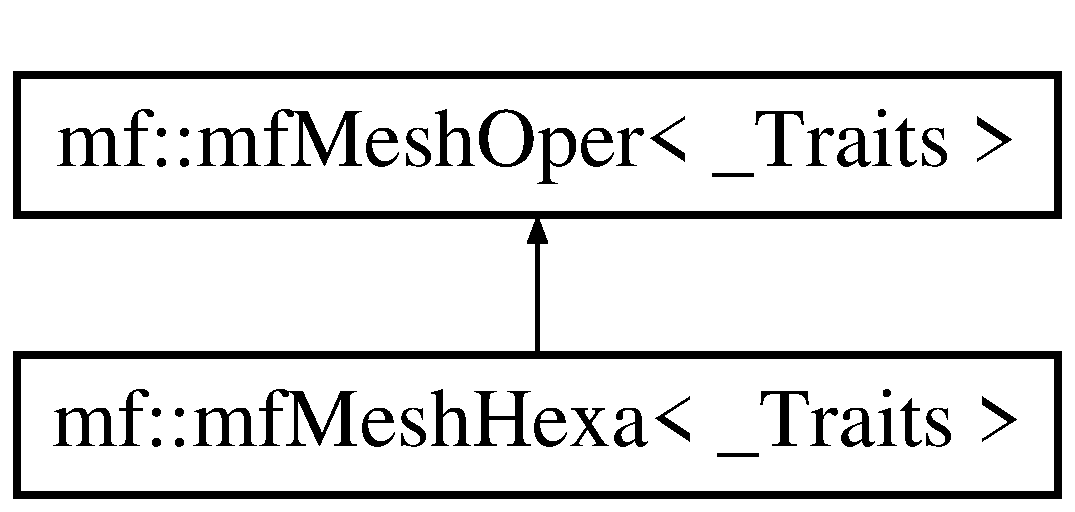
\includegraphics[height=2.000000cm]{classmf_1_1mfMeshHexa}
\end{center}
\end{figure}
\subsection*{Public Types}
\begin{DoxyCompactItemize}
\item 
typedef \_\-Traits::ids \hyperlink{classmf_1_1mfMeshHexa_ab95eac5745c5efd075cf732421c40d94}{ids}
\item 
\hypertarget{classmf_1_1mfMeshHexa_a079b3030e947801ec2ae45637db567ad}{
typedef \_\-Traits::sVertex {\bfseries sVertex}}
\label{classmf_1_1mfMeshHexa_a079b3030e947801ec2ae45637db567ad}

\item 
\hypertarget{classmf_1_1mfMeshHexa_a2788d6dc9ab468e6d363b1e8395eb615}{
typedef \_\-Traits::sCell {\bfseries sCell}}
\label{classmf_1_1mfMeshHexa_a2788d6dc9ab468e6d363b1e8395eb615}

\item 
\hypertarget{classmf_1_1mfMeshHexa_adf835487b92643f0bb47b232a301a440}{
typedef \_\-Traits::sGeometric {\bfseries sGeometric}}
\label{classmf_1_1mfMeshHexa_adf835487b92643f0bb47b232a301a440}

\item 
\hypertarget{classmf_1_1mfMeshHexa_aef7339b0da506d763cc113da810987ba}{
typedef \hyperlink{classmf_1_1mfSing}{mfSing}$<$ \_\-Traits $>$ {\bfseries sSing}}
\label{classmf_1_1mfMeshHexa_aef7339b0da506d763cc113da810987ba}

\item 
typedef \_\-Traits::sMesh \hyperlink{classmf_1_1mfMeshHexa_adc5f7c62030d948caf1f04a255f385de}{sMesh}
\end{DoxyCompactItemize}
\subsection*{Public Member Functions}
\begin{DoxyCompactItemize}
\item 
\hyperlink{classmf_1_1mfMeshHexa_adb23c1c168b7d84af3029306fe621711}{mfMeshHexa} (\hyperlink{classmf_1_1mfMeshHexa_adc5f7c62030d948caf1f04a255f385de}{sMesh} $\ast$\_\-mesh)
\item 
\hyperlink{classmf_1_1mfMeshHexa_ae0dc24a89e171a408e4e5ebe91c31132}{$\sim$mfMeshHexa} ()
\item 
void \hyperlink{classmf_1_1mfMeshHexa_ad9b87bd8f3042eb791dfbb41403fc2e3}{addCell} (\hyperlink{classmf_1_1mfMeshHexa_ab95eac5745c5efd075cf732421c40d94}{ids} idcell, \hyperlink{classmf_1_1mfMeshHexa_ab95eac5745c5efd075cf732421c40d94}{ids} $\ast$idvertices MF\_\-DMUTEXVD)
\item 
void \hyperlink{classmf_1_1mfMeshHexa_aa1edfd7f7763a08e0bd9f86065e3a8bd}{delCell} (\hyperlink{classmf_1_1mfMeshHexa_ab95eac5745c5efd075cf732421c40d94}{ids} idcell MF\_\-DMUTEXVD)
\end{DoxyCompactItemize}


\subsection{Detailed Description}
\subsubsection*{template$<$class \_\-Traits$>$ class mf::mfMeshHexa$<$ \_\-Traits $>$}

Operation Class for Hexaedra in 3D space (with not oriented vertices)

\_\-Traits must have: ids, sVertex, sCell, sSing, sMesh 

\subsection{Member Typedef Documentation}
\hypertarget{classmf_1_1mfMeshHexa_ab95eac5745c5efd075cf732421c40d94}{
\index{mf::mfMeshHexa@{mf::mfMeshHexa}!ids@{ids}}
\index{ids@{ids}!mf::mfMeshHexa@{mf::mfMeshHexa}}
\subsubsection[{ids}]{\setlength{\rightskip}{0pt plus 5cm}template$<$class \_\-Traits $>$ typedef \_\-Traits::ids {\bf mf::mfMeshHexa}$<$ \_\-Traits $>$::{\bf ids}}}
\label{classmf_1_1mfMeshHexa_ab95eac5745c5efd075cf732421c40d94}
Id typename definition 

Reimplemented from \hyperlink{classmf_1_1mfMeshOper_a526d1466339244781fbdc0dbfe5ad210}{mf::mfMeshOper$<$ \_\-Traits $>$}.

\hypertarget{classmf_1_1mfMeshHexa_adc5f7c62030d948caf1f04a255f385de}{
\index{mf::mfMeshHexa@{mf::mfMeshHexa}!sMesh@{sMesh}}
\index{sMesh@{sMesh}!mf::mfMeshHexa@{mf::mfMeshHexa}}
\subsubsection[{sMesh}]{\setlength{\rightskip}{0pt plus 5cm}template$<$class \_\-Traits $>$ typedef \_\-Traits::sMesh {\bf mf::mfMeshHexa}$<$ \_\-Traits $>$::{\bf sMesh}}}
\label{classmf_1_1mfMeshHexa_adc5f7c62030d948caf1f04a255f385de}
Mesh typename definition 

Reimplemented from \hyperlink{classmf_1_1mfMeshOper_a96c05da9a054cf9ac58d15211922f936}{mf::mfMeshOper$<$ \_\-Traits $>$}.



\subsection{Constructor \& Destructor Documentation}
\hypertarget{classmf_1_1mfMeshHexa_adb23c1c168b7d84af3029306fe621711}{
\index{mf::mfMeshHexa@{mf::mfMeshHexa}!mfMeshHexa@{mfMeshHexa}}
\index{mfMeshHexa@{mfMeshHexa}!mf::mfMeshHexa@{mf::mfMeshHexa}}
\subsubsection[{mfMeshHexa}]{\setlength{\rightskip}{0pt plus 5cm}template$<$class \_\-Traits $>$ {\bf mf::mfMeshHexa}$<$ \_\-Traits $>$::{\bf mfMeshHexa} (
\begin{DoxyParamCaption}
\item[{{\bf sMesh} $\ast$}]{\_\-mesh}
\end{DoxyParamCaption}
)}}
\label{classmf_1_1mfMeshHexa_adb23c1c168b7d84af3029306fe621711}
Constructor


\begin{DoxyParams}{Parameters}
{\em \_\-mesh,:} & the mesh address that this class will manipulate \\
\hline
\end{DoxyParams}
\hypertarget{classmf_1_1mfMeshHexa_ae0dc24a89e171a408e4e5ebe91c31132}{
\index{mf::mfMeshHexa@{mf::mfMeshHexa}!$\sim$mfMeshHexa@{$\sim$mfMeshHexa}}
\index{$\sim$mfMeshHexa@{$\sim$mfMeshHexa}!mf::mfMeshHexa@{mf::mfMeshHexa}}
\subsubsection[{$\sim$mfMeshHexa}]{\setlength{\rightskip}{0pt plus 5cm}template$<$class \_\-Traits $>$ {\bf mf::mfMeshHexa}$<$ \_\-Traits $>$::$\sim${\bf mfMeshHexa} (
\begin{DoxyParamCaption}
{}
\end{DoxyParamCaption}
)}}
\label{classmf_1_1mfMeshHexa_ae0dc24a89e171a408e4e5ebe91c31132}
Destructor 

\subsection{Member Function Documentation}
\hypertarget{classmf_1_1mfMeshHexa_ad9b87bd8f3042eb791dfbb41403fc2e3}{
\index{mf::mfMeshHexa@{mf::mfMeshHexa}!addCell@{addCell}}
\index{addCell@{addCell}!mf::mfMeshHexa@{mf::mfMeshHexa}}
\subsubsection[{addCell}]{\setlength{\rightskip}{0pt plus 5cm}template$<$class \_\-Traits $>$ void {\bf mf::mfMeshHexa}$<$ \_\-Traits $>$::addCell (
\begin{DoxyParamCaption}
\item[{{\bf ids}}]{idcell, }
\item[{{\bf ids} $\ast$idvertices}]{MF\_\-DMUTEXVD}
\end{DoxyParamCaption}
)}}
\label{classmf_1_1mfMeshHexa_ad9b87bd8f3042eb791dfbb41403fc2e3}
Add cell in mesh


\begin{DoxyParams}{Parameters}
{\em idcell,:} & cell id \\
\hline
{\em idvertices,:} & vector with vertices ids of the cell \\
\hline
\end{DoxyParams}
\hypertarget{classmf_1_1mfMeshHexa_aa1edfd7f7763a08e0bd9f86065e3a8bd}{
\index{mf::mfMeshHexa@{mf::mfMeshHexa}!delCell@{delCell}}
\index{delCell@{delCell}!mf::mfMeshHexa@{mf::mfMeshHexa}}
\subsubsection[{delCell}]{\setlength{\rightskip}{0pt plus 5cm}template$<$class \_\-Traits $>$ void {\bf mf::mfMeshHexa}$<$ \_\-Traits $>$::delCell (
\begin{DoxyParamCaption}
\item[{{\bf ids} idcell}]{MF\_\-DMUTEXVD}
\end{DoxyParamCaption}
)}}
\label{classmf_1_1mfMeshHexa_aa1edfd7f7763a08e0bd9f86065e3a8bd}
Delete a cell


\begin{DoxyParams}{Parameters}
{\em idcell,:} & cell id \\
\hline
\end{DoxyParams}


The documentation for this class was generated from the following file:\begin{DoxyCompactItemize}
\item 
mfMeshHexa.h\end{DoxyCompactItemize}

\hypertarget{classmf_1_1mfMeshHybridSurface}{
\section{mf::mfMeshHybridSurface$<$ \_\-Traits $>$ Class Template Reference}
\label{classmf_1_1mfMeshHybridSurface}\index{mf::mfMeshHybridSurface@{mf::mfMeshHybridSurface}}
}


{\ttfamily \#include $<$mfMeshHybridSurface.h$>$}

Inheritance diagram for mf::mfMeshHybridSurface$<$ \_\-Traits $>$:\begin{figure}[H]
\begin{center}
\leavevmode
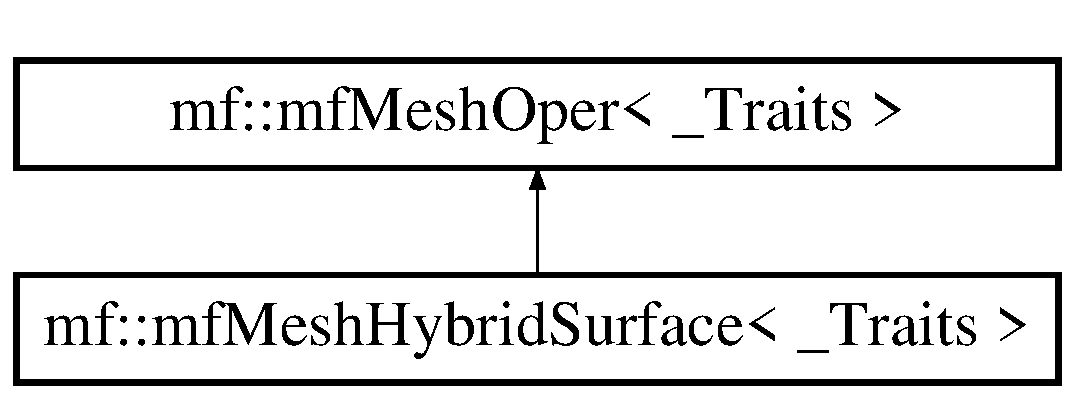
\includegraphics[height=2.000000cm]{classmf_1_1mfMeshHybridSurface}
\end{center}
\end{figure}
\subsection*{Public Types}
\begin{DoxyCompactItemize}
\item 
typedef \_\-Traits::ids \hyperlink{classmf_1_1mfMeshHybridSurface_a46dd7994ecadd8ead204ab52dcb632ca}{ids}
\item 
typedef \_\-Traits::sVertex \hyperlink{classmf_1_1mfMeshHybridSurface_a3739f5c613f7c0fce7946c0f4fdeeb1b}{sVertex}
\item 
typedef \_\-Traits::sCell \hyperlink{classmf_1_1mfMeshHybridSurface_ae8effc64c1dfb9b88223478812400505}{sCell}
\item 
typedef \hyperlink{classmf_1_1mfSing}{mfSing}$<$ \_\-Traits $>$ \hyperlink{classmf_1_1mfMeshHybridSurface_ac9e0a04d9e5f9cf40d751f7661ac9a7a}{sSing}
\item 
typedef \_\-Traits::sMesh \hyperlink{classmf_1_1mfMeshHybridSurface_a204a2dcbd0802b263253055d7d2d1b9a}{sMesh}
\end{DoxyCompactItemize}
\subsection*{Public Member Functions}
\begin{DoxyCompactItemize}
\item 
\hyperlink{classmf_1_1mfMeshHybridSurface_afa40a6d452119c868d4996e3ec42dc0a}{mfMeshHybridSurface} (\hyperlink{classmf_1_1mfMeshHybridSurface_a204a2dcbd0802b263253055d7d2d1b9a}{sMesh} $\ast$\_\-mesh)
\item 
\hyperlink{classmf_1_1mfMeshHybridSurface_af72771dbaf0d5235ade66fe38308f872}{$\sim$mfMeshHybridSurface} ()
\item 
void \hyperlink{classmf_1_1mfMeshHybridSurface_a970d678d03168429e492eed98064602f}{addCell} (\hyperlink{classmf_1_1mfMeshHybridSurface_a46dd7994ecadd8ead204ab52dcb632ca}{ids} idcell, \hyperlink{classmf_1_1mfMeshHybridSurface_a46dd7994ecadd8ead204ab52dcb632ca}{ids} $\ast$idvertices MF\_\-DMUTEXVD)
\item 
void \hyperlink{classmf_1_1mfMeshHybridSurface_aa6726532e75edd42143a477d4036f9ad}{delCell} (\hyperlink{classmf_1_1mfMeshHybridSurface_a46dd7994ecadd8ead204ab52dcb632ca}{ids} idcell MF\_\-DMUTEXVD)
\end{DoxyCompactItemize}


\subsection{Detailed Description}
\subsubsection*{template$<$class \_\-Traits$>$ class mf::mfMeshHybridSurface$<$ \_\-Traits $>$}

Operation Class for Hybrid Surface in a 3D space (with oriented quadrilaterals)

\_\-Traits must have: ids, sVertex, sCell, sSing, sMesh 

\subsection{Member Typedef Documentation}
\hypertarget{classmf_1_1mfMeshHybridSurface_a46dd7994ecadd8ead204ab52dcb632ca}{
\index{mf::mfMeshHybridSurface@{mf::mfMeshHybridSurface}!ids@{ids}}
\index{ids@{ids}!mf::mfMeshHybridSurface@{mf::mfMeshHybridSurface}}
\subsubsection[{ids}]{\setlength{\rightskip}{0pt plus 5cm}template$<$class \_\-Traits $>$ typedef \_\-Traits::ids {\bf mf::mfMeshHybridSurface}$<$ \_\-Traits $>$::{\bf ids}}}
\label{classmf_1_1mfMeshHybridSurface_a46dd7994ecadd8ead204ab52dcb632ca}
Id typename definition 

Reimplemented from \hyperlink{classmf_1_1mfMeshOper_a526d1466339244781fbdc0dbfe5ad210}{mf::mfMeshOper$<$ \_\-Traits $>$}.

\hypertarget{classmf_1_1mfMeshHybridSurface_ae8effc64c1dfb9b88223478812400505}{
\index{mf::mfMeshHybridSurface@{mf::mfMeshHybridSurface}!sCell@{sCell}}
\index{sCell@{sCell}!mf::mfMeshHybridSurface@{mf::mfMeshHybridSurface}}
\subsubsection[{sCell}]{\setlength{\rightskip}{0pt plus 5cm}template$<$class \_\-Traits $>$ typedef \_\-Traits::sCell {\bf mf::mfMeshHybridSurface}$<$ \_\-Traits $>$::{\bf sCell}}}
\label{classmf_1_1mfMeshHybridSurface_ae8effc64c1dfb9b88223478812400505}
Cell typename definition \hypertarget{classmf_1_1mfMeshHybridSurface_a204a2dcbd0802b263253055d7d2d1b9a}{
\index{mf::mfMeshHybridSurface@{mf::mfMeshHybridSurface}!sMesh@{sMesh}}
\index{sMesh@{sMesh}!mf::mfMeshHybridSurface@{mf::mfMeshHybridSurface}}
\subsubsection[{sMesh}]{\setlength{\rightskip}{0pt plus 5cm}template$<$class \_\-Traits $>$ typedef \_\-Traits::sMesh {\bf mf::mfMeshHybridSurface}$<$ \_\-Traits $>$::{\bf sMesh}}}
\label{classmf_1_1mfMeshHybridSurface_a204a2dcbd0802b263253055d7d2d1b9a}
Mesh typename definition 

Reimplemented from \hyperlink{classmf_1_1mfMeshOper_a96c05da9a054cf9ac58d15211922f936}{mf::mfMeshOper$<$ \_\-Traits $>$}.

\hypertarget{classmf_1_1mfMeshHybridSurface_ac9e0a04d9e5f9cf40d751f7661ac9a7a}{
\index{mf::mfMeshHybridSurface@{mf::mfMeshHybridSurface}!sSing@{sSing}}
\index{sSing@{sSing}!mf::mfMeshHybridSurface@{mf::mfMeshHybridSurface}}
\subsubsection[{sSing}]{\setlength{\rightskip}{0pt plus 5cm}template$<$class \_\-Traits $>$ typedef {\bf mfSing}$<$\_\-Traits$>$ {\bf mf::mfMeshHybridSurface}$<$ \_\-Traits $>$::{\bf sSing}}}
\label{classmf_1_1mfMeshHybridSurface_ac9e0a04d9e5f9cf40d751f7661ac9a7a}
Singular typename definition \hypertarget{classmf_1_1mfMeshHybridSurface_a3739f5c613f7c0fce7946c0f4fdeeb1b}{
\index{mf::mfMeshHybridSurface@{mf::mfMeshHybridSurface}!sVertex@{sVertex}}
\index{sVertex@{sVertex}!mf::mfMeshHybridSurface@{mf::mfMeshHybridSurface}}
\subsubsection[{sVertex}]{\setlength{\rightskip}{0pt plus 5cm}template$<$class \_\-Traits $>$ typedef \_\-Traits::sVertex {\bf mf::mfMeshHybridSurface}$<$ \_\-Traits $>$::{\bf sVertex}}}
\label{classmf_1_1mfMeshHybridSurface_a3739f5c613f7c0fce7946c0f4fdeeb1b}
Vertex typename definition 

\subsection{Constructor \& Destructor Documentation}
\hypertarget{classmf_1_1mfMeshHybridSurface_afa40a6d452119c868d4996e3ec42dc0a}{
\index{mf::mfMeshHybridSurface@{mf::mfMeshHybridSurface}!mfMeshHybridSurface@{mfMeshHybridSurface}}
\index{mfMeshHybridSurface@{mfMeshHybridSurface}!mf::mfMeshHybridSurface@{mf::mfMeshHybridSurface}}
\subsubsection[{mfMeshHybridSurface}]{\setlength{\rightskip}{0pt plus 5cm}template$<$class \_\-Traits $>$ {\bf mf::mfMeshHybridSurface}$<$ \_\-Traits $>$::{\bf mfMeshHybridSurface} (
\begin{DoxyParamCaption}
\item[{{\bf sMesh} $\ast$}]{\_\-mesh}
\end{DoxyParamCaption}
)}}
\label{classmf_1_1mfMeshHybridSurface_afa40a6d452119c868d4996e3ec42dc0a}
Constructor


\begin{DoxyParams}{Parameters}
{\em \_\-mesh,:} & the mesh address that this class will manipulate \\
\hline
\end{DoxyParams}
\hypertarget{classmf_1_1mfMeshHybridSurface_af72771dbaf0d5235ade66fe38308f872}{
\index{mf::mfMeshHybridSurface@{mf::mfMeshHybridSurface}!$\sim$mfMeshHybridSurface@{$\sim$mfMeshHybridSurface}}
\index{$\sim$mfMeshHybridSurface@{$\sim$mfMeshHybridSurface}!mf::mfMeshHybridSurface@{mf::mfMeshHybridSurface}}
\subsubsection[{$\sim$mfMeshHybridSurface}]{\setlength{\rightskip}{0pt plus 5cm}template$<$class \_\-Traits $>$ {\bf mf::mfMeshHybridSurface}$<$ \_\-Traits $>$::$\sim${\bf mfMeshHybridSurface} (
\begin{DoxyParamCaption}
{}
\end{DoxyParamCaption}
)}}
\label{classmf_1_1mfMeshHybridSurface_af72771dbaf0d5235ade66fe38308f872}
Destructor 

\subsection{Member Function Documentation}
\hypertarget{classmf_1_1mfMeshHybridSurface_a970d678d03168429e492eed98064602f}{
\index{mf::mfMeshHybridSurface@{mf::mfMeshHybridSurface}!addCell@{addCell}}
\index{addCell@{addCell}!mf::mfMeshHybridSurface@{mf::mfMeshHybridSurface}}
\subsubsection[{addCell}]{\setlength{\rightskip}{0pt plus 5cm}template$<$class \_\-Traits $>$ void {\bf mf::mfMeshHybridSurface}$<$ \_\-Traits $>$::addCell (
\begin{DoxyParamCaption}
\item[{{\bf ids}}]{idcell, }
\item[{{\bf ids} $\ast$idvertices}]{MF\_\-DMUTEXVD}
\end{DoxyParamCaption}
)}}
\label{classmf_1_1mfMeshHybridSurface_a970d678d03168429e492eed98064602f}
Add cell in mesh


\begin{DoxyParams}{Parameters}
{\em idcell,:} & cell id \\
\hline
{\em idvertices,:} & vector with vertices ids of the cell \\
\hline
\end{DoxyParams}
\hypertarget{classmf_1_1mfMeshHybridSurface_aa6726532e75edd42143a477d4036f9ad}{
\index{mf::mfMeshHybridSurface@{mf::mfMeshHybridSurface}!delCell@{delCell}}
\index{delCell@{delCell}!mf::mfMeshHybridSurface@{mf::mfMeshHybridSurface}}
\subsubsection[{delCell}]{\setlength{\rightskip}{0pt plus 5cm}template$<$class \_\-Traits $>$ void {\bf mf::mfMeshHybridSurface}$<$ \_\-Traits $>$::delCell (
\begin{DoxyParamCaption}
\item[{{\bf ids} idcell}]{MF\_\-DMUTEXVD}
\end{DoxyParamCaption}
)}}
\label{classmf_1_1mfMeshHybridSurface_aa6726532e75edd42143a477d4036f9ad}
Delete a cell


\begin{DoxyParams}{Parameters}
{\em idcell,:} & cell id \\
\hline
\end{DoxyParams}


The documentation for this class was generated from the following file:\begin{DoxyCompactItemize}
\item 
mfMeshHybridSurface.h\end{DoxyCompactItemize}

\hypertarget{classmf_1_1mfMeshNOSurface}{
\section{mf::mfMeshNOSurface$<$ \_\-Traits $>$ Class Template Reference}
\label{classmf_1_1mfMeshNOSurface}\index{mf::mfMeshNOSurface@{mf::mfMeshNOSurface}}
}


{\ttfamily \#include $<$mfMeshNOSurface.h$>$}

Inheritance diagram for mf::mfMeshNOSurface$<$ \_\-Traits $>$:\begin{figure}[H]
\begin{center}
\leavevmode
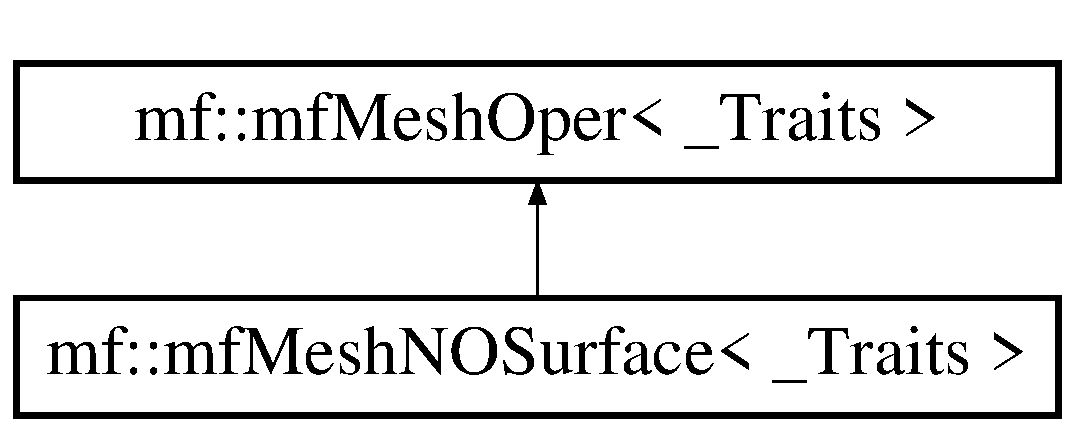
\includegraphics[height=2.000000cm]{classmf_1_1mfMeshNOSurface}
\end{center}
\end{figure}
\subsection*{Public Types}
\begin{DoxyCompactItemize}
\item 
typedef \_\-Traits::ids \hyperlink{classmf_1_1mfMeshNOSurface_afee75f2d037d52e9a164fca832091c9b}{ids}
\item 
\hypertarget{classmf_1_1mfMeshNOSurface_a64fc49ba31ca5846cb969890573053bb}{
typedef \_\-Traits::sVertex {\bfseries sVertex}}
\label{classmf_1_1mfMeshNOSurface_a64fc49ba31ca5846cb969890573053bb}

\item 
\hypertarget{classmf_1_1mfMeshNOSurface_a2fa1df913ec1d90af922ece363bcfef1}{
typedef \_\-Traits::sCell {\bfseries sCell}}
\label{classmf_1_1mfMeshNOSurface_a2fa1df913ec1d90af922ece363bcfef1}

\item 
\hypertarget{classmf_1_1mfMeshNOSurface_a5a69aa6fc01bfba39c6161159612c8ef}{
typedef \hyperlink{classmf_1_1mfSing}{mfSing}$<$ \_\-Traits $>$ {\bfseries sSing}}
\label{classmf_1_1mfMeshNOSurface_a5a69aa6fc01bfba39c6161159612c8ef}

\item 
typedef \_\-Traits::sMesh \hyperlink{classmf_1_1mfMeshNOSurface_af5a7f4fc5fe7b228d1e96f5f37ee2dba}{sMesh}
\end{DoxyCompactItemize}
\subsection*{Public Member Functions}
\begin{DoxyCompactItemize}
\item 
\hyperlink{classmf_1_1mfMeshNOSurface_a776a623404f1ecce3aace8b1145d3def}{mfMeshNOSurface} (\hyperlink{classmf_1_1mfMeshNOSurface_af5a7f4fc5fe7b228d1e96f5f37ee2dba}{sMesh} $\ast$\_\-mesh)
\item 
\hyperlink{classmf_1_1mfMeshNOSurface_a90acaff3afe1d229d9a00e4e60ff58f8}{$\sim$mfMeshNOSurface} ()
\item 
void \hyperlink{classmf_1_1mfMeshNOSurface_abd06139730cbcaa8d476f08abe4f93c0}{addCell} (\hyperlink{classmf_1_1mfMeshNOSurface_afee75f2d037d52e9a164fca832091c9b}{ids} idcell, \hyperlink{classmf_1_1mfMeshNOSurface_afee75f2d037d52e9a164fca832091c9b}{ids} $\ast$idvertices MF\_\-DMUTEXVD)
\item 
void \hyperlink{classmf_1_1mfMeshNOSurface_ab10b57f868ebc3e513e64b8395f6dfed}{delCell} (\hyperlink{classmf_1_1mfMeshNOSurface_afee75f2d037d52e9a164fca832091c9b}{ids} idcell MF\_\-DMUTEXVD)
\end{DoxyCompactItemize}


\subsection{Detailed Description}
\subsubsection*{template$<$class \_\-Traits$>$ class mf::mfMeshNOSurface$<$ \_\-Traits $>$}

Operation Class for Triangles in 3D space (with not oriented triangles)

\_\-Traits must have: ids, sVertex, sCell, sSing, sMesh 

\subsection{Member Typedef Documentation}
\hypertarget{classmf_1_1mfMeshNOSurface_afee75f2d037d52e9a164fca832091c9b}{
\index{mf::mfMeshNOSurface@{mf::mfMeshNOSurface}!ids@{ids}}
\index{ids@{ids}!mf::mfMeshNOSurface@{mf::mfMeshNOSurface}}
\subsubsection[{ids}]{\setlength{\rightskip}{0pt plus 5cm}template$<$class \_\-Traits $>$ typedef \_\-Traits::ids {\bf mf::mfMeshNOSurface}$<$ \_\-Traits $>$::{\bf ids}}}
\label{classmf_1_1mfMeshNOSurface_afee75f2d037d52e9a164fca832091c9b}
Id typename definition 

Reimplemented from \hyperlink{classmf_1_1mfMeshOper_a526d1466339244781fbdc0dbfe5ad210}{mf::mfMeshOper$<$ \_\-Traits $>$}.

\hypertarget{classmf_1_1mfMeshNOSurface_af5a7f4fc5fe7b228d1e96f5f37ee2dba}{
\index{mf::mfMeshNOSurface@{mf::mfMeshNOSurface}!sMesh@{sMesh}}
\index{sMesh@{sMesh}!mf::mfMeshNOSurface@{mf::mfMeshNOSurface}}
\subsubsection[{sMesh}]{\setlength{\rightskip}{0pt plus 5cm}template$<$class \_\-Traits $>$ typedef \_\-Traits::sMesh {\bf mf::mfMeshNOSurface}$<$ \_\-Traits $>$::{\bf sMesh}}}
\label{classmf_1_1mfMeshNOSurface_af5a7f4fc5fe7b228d1e96f5f37ee2dba}
Mesh typename definition 

Reimplemented from \hyperlink{classmf_1_1mfMeshOper_a96c05da9a054cf9ac58d15211922f936}{mf::mfMeshOper$<$ \_\-Traits $>$}.



\subsection{Constructor \& Destructor Documentation}
\hypertarget{classmf_1_1mfMeshNOSurface_a776a623404f1ecce3aace8b1145d3def}{
\index{mf::mfMeshNOSurface@{mf::mfMeshNOSurface}!mfMeshNOSurface@{mfMeshNOSurface}}
\index{mfMeshNOSurface@{mfMeshNOSurface}!mf::mfMeshNOSurface@{mf::mfMeshNOSurface}}
\subsubsection[{mfMeshNOSurface}]{\setlength{\rightskip}{0pt plus 5cm}template$<$class \_\-Traits $>$ {\bf mf::mfMeshNOSurface}$<$ \_\-Traits $>$::{\bf mfMeshNOSurface} (
\begin{DoxyParamCaption}
\item[{{\bf sMesh} $\ast$}]{\_\-mesh}
\end{DoxyParamCaption}
)}}
\label{classmf_1_1mfMeshNOSurface_a776a623404f1ecce3aace8b1145d3def}
Constructor


\begin{DoxyParams}{Parameters}
{\em \_\-mesh,:} & the mesh address that this class will manipulate \\
\hline
\end{DoxyParams}
\hypertarget{classmf_1_1mfMeshNOSurface_a90acaff3afe1d229d9a00e4e60ff58f8}{
\index{mf::mfMeshNOSurface@{mf::mfMeshNOSurface}!$\sim$mfMeshNOSurface@{$\sim$mfMeshNOSurface}}
\index{$\sim$mfMeshNOSurface@{$\sim$mfMeshNOSurface}!mf::mfMeshNOSurface@{mf::mfMeshNOSurface}}
\subsubsection[{$\sim$mfMeshNOSurface}]{\setlength{\rightskip}{0pt plus 5cm}template$<$class \_\-Traits $>$ {\bf mf::mfMeshNOSurface}$<$ \_\-Traits $>$::$\sim${\bf mfMeshNOSurface} (
\begin{DoxyParamCaption}
{}
\end{DoxyParamCaption}
)}}
\label{classmf_1_1mfMeshNOSurface_a90acaff3afe1d229d9a00e4e60ff58f8}
Destructor 

\subsection{Member Function Documentation}
\hypertarget{classmf_1_1mfMeshNOSurface_abd06139730cbcaa8d476f08abe4f93c0}{
\index{mf::mfMeshNOSurface@{mf::mfMeshNOSurface}!addCell@{addCell}}
\index{addCell@{addCell}!mf::mfMeshNOSurface@{mf::mfMeshNOSurface}}
\subsubsection[{addCell}]{\setlength{\rightskip}{0pt plus 5cm}template$<$class \_\-Traits $>$ void {\bf mf::mfMeshNOSurface}$<$ \_\-Traits $>$::addCell (
\begin{DoxyParamCaption}
\item[{{\bf ids}}]{idcell, }
\item[{{\bf ids} $\ast$idvertices}]{MF\_\-DMUTEXVD}
\end{DoxyParamCaption}
)}}
\label{classmf_1_1mfMeshNOSurface_abd06139730cbcaa8d476f08abe4f93c0}
Add cell in mesh


\begin{DoxyParams}{Parameters}
{\em idcell,:} & cell id \\
\hline
{\em idvertices,:} & vector with vertices ids of the cell \\
\hline
\end{DoxyParams}
\hypertarget{classmf_1_1mfMeshNOSurface_ab10b57f868ebc3e513e64b8395f6dfed}{
\index{mf::mfMeshNOSurface@{mf::mfMeshNOSurface}!delCell@{delCell}}
\index{delCell@{delCell}!mf::mfMeshNOSurface@{mf::mfMeshNOSurface}}
\subsubsection[{delCell}]{\setlength{\rightskip}{0pt plus 5cm}template$<$class \_\-Traits $>$ void {\bf mf::mfMeshNOSurface}$<$ \_\-Traits $>$::delCell (
\begin{DoxyParamCaption}
\item[{{\bf ids} idcell}]{MF\_\-DMUTEXVD}
\end{DoxyParamCaption}
)}}
\label{classmf_1_1mfMeshNOSurface_ab10b57f868ebc3e513e64b8395f6dfed}
Delete a cell


\begin{DoxyParams}{Parameters}
{\em idcell,:} & cell id \\
\hline
\end{DoxyParams}


The documentation for this class was generated from the following file:\begin{DoxyCompactItemize}
\item 
mfMeshNOSurface.h\end{DoxyCompactItemize}

\hypertarget{classmf_1_1mfMeshOper}{
\section{mf::mfMeshOper$<$ \_\-Traits $>$ Class Template Reference}
\label{classmf_1_1mfMeshOper}\index{mf::mfMeshOper@{mf::mfMeshOper}}
}


{\ttfamily \#include $<$mfMeshOper.h$>$}

Inheritance diagram for mf::mfMeshOper$<$ \_\-Traits $>$:\begin{figure}[H]
\begin{center}
\leavevmode
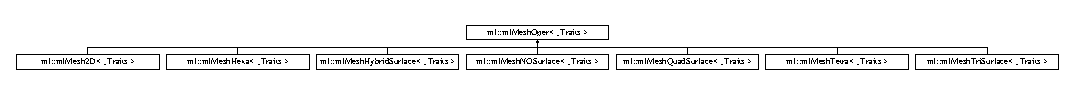
\includegraphics[height=0.701754cm]{classmf_1_1mfMeshOper}
\end{center}
\end{figure}
\subsection*{Public Types}
\begin{DoxyCompactItemize}
\item 
typedef \_\-Traits::ids \hyperlink{classmf_1_1mfMeshOper_a526d1466339244781fbdc0dbfe5ad210}{ids}
\item 
typedef \_\-Traits::sMesh \hyperlink{classmf_1_1mfMeshOper_a96c05da9a054cf9ac58d15211922f936}{sMesh}
\end{DoxyCompactItemize}
\subsection*{Protected Member Functions}
\begin{DoxyCompactItemize}
\item 
\hyperlink{classmf_1_1mfMeshOper_a902c507f17a7a2d8d47c3dcc5f1e2686}{mfMeshOper} (\hyperlink{classmf_1_1mfMeshOper_a96c05da9a054cf9ac58d15211922f936}{sMesh} $\ast$\_\-mesh)
\item 
\hyperlink{classmf_1_1mfMeshOper_a31338779fec74743fe804882e1e0ba59}{$\sim$mfMeshOper} ()
\end{DoxyCompactItemize}
\subsection*{Protected Attributes}
\begin{DoxyCompactItemize}
\item 
\hypertarget{classmf_1_1mfMeshOper_a5d2bd1d40dd638444d5047dd42d5ca6a}{
\hyperlink{classmf_1_1mfMeshOper_a96c05da9a054cf9ac58d15211922f936}{sMesh} $\ast$ {\bfseries mesh}}
\label{classmf_1_1mfMeshOper_a5d2bd1d40dd638444d5047dd42d5ca6a}

\end{DoxyCompactItemize}


\subsection{Detailed Description}
\subsubsection*{template$<$class \_\-Traits$>$ class mf::mfMeshOper$<$ \_\-Traits $>$}

Base Operation Class for \hyperlink{classmf_1_1mfMesh}{mfMesh}

\_\-Traits must have: ids, sMesh 

\subsection{Member Typedef Documentation}
\hypertarget{classmf_1_1mfMeshOper_a526d1466339244781fbdc0dbfe5ad210}{
\index{mf::mfMeshOper@{mf::mfMeshOper}!ids@{ids}}
\index{ids@{ids}!mf::mfMeshOper@{mf::mfMeshOper}}
\subsubsection[{ids}]{\setlength{\rightskip}{0pt plus 5cm}template$<$class \_\-Traits $>$ typedef \_\-Traits::ids {\bf mf::mfMeshOper}$<$ \_\-Traits $>$::{\bf ids}}}
\label{classmf_1_1mfMeshOper_a526d1466339244781fbdc0dbfe5ad210}
Id typename definition 

Reimplemented in \hyperlink{classmf_1_1mfMesh2D_a517d508b5d1959b3c697f7c393ccd068}{mf::mfMesh2D$<$ \_\-Traits $>$}, \hyperlink{classmf_1_1mfMeshHexa_ab95eac5745c5efd075cf732421c40d94}{mf::mfMeshHexa$<$ \_\-Traits $>$}, \hyperlink{classmf_1_1mfMeshHybridSurface_a46dd7994ecadd8ead204ab52dcb632ca}{mf::mfMeshHybridSurface$<$ \_\-Traits $>$}, \hyperlink{classmf_1_1mfMeshNOSurface_afee75f2d037d52e9a164fca832091c9b}{mf::mfMeshNOSurface$<$ \_\-Traits $>$}, \hyperlink{classmf_1_1mfMeshQuadSurface_a91f8c5a330192db329f7b2e116b9149d}{mf::mfMeshQuadSurface$<$ \_\-Traits $>$}, \hyperlink{classmf_1_1mfMeshTetra_adbcfde79b2f9076ed56ea0e373508967}{mf::mfMeshTetra$<$ \_\-Traits $>$}, and \hyperlink{classmf_1_1mfMeshTriSurface_a2432b4eb1b385605e96d17e2774519f5}{mf::mfMeshTriSurface$<$ \_\-Traits $>$}.

\hypertarget{classmf_1_1mfMeshOper_a96c05da9a054cf9ac58d15211922f936}{
\index{mf::mfMeshOper@{mf::mfMeshOper}!sMesh@{sMesh}}
\index{sMesh@{sMesh}!mf::mfMeshOper@{mf::mfMeshOper}}
\subsubsection[{sMesh}]{\setlength{\rightskip}{0pt plus 5cm}template$<$class \_\-Traits $>$ typedef \_\-Traits::sMesh {\bf mf::mfMeshOper}$<$ \_\-Traits $>$::{\bf sMesh}}}
\label{classmf_1_1mfMeshOper_a96c05da9a054cf9ac58d15211922f936}
Mesh typename definition 

Reimplemented in \hyperlink{classmf_1_1mfMesh2D_aa197f7f92e5aa8e68703a5eeb3d9ae04}{mf::mfMesh2D$<$ \_\-Traits $>$}, \hyperlink{classmf_1_1mfMeshHexa_adc5f7c62030d948caf1f04a255f385de}{mf::mfMeshHexa$<$ \_\-Traits $>$}, \hyperlink{classmf_1_1mfMeshHybridSurface_a204a2dcbd0802b263253055d7d2d1b9a}{mf::mfMeshHybridSurface$<$ \_\-Traits $>$}, \hyperlink{classmf_1_1mfMeshNOSurface_af5a7f4fc5fe7b228d1e96f5f37ee2dba}{mf::mfMeshNOSurface$<$ \_\-Traits $>$}, \hyperlink{classmf_1_1mfMeshQuadSurface_a5c71a1c02ec20c5c33393f8bd256168d}{mf::mfMeshQuadSurface$<$ \_\-Traits $>$}, \hyperlink{classmf_1_1mfMeshTetra_a1b1ccf8633127e7307c35b150a522193}{mf::mfMeshTetra$<$ \_\-Traits $>$}, and \hyperlink{classmf_1_1mfMeshTriSurface_aa25d8c016f15b0073c5ba5aa0a64be86}{mf::mfMeshTriSurface$<$ \_\-Traits $>$}.



\subsection{Constructor \& Destructor Documentation}
\hypertarget{classmf_1_1mfMeshOper_a902c507f17a7a2d8d47c3dcc5f1e2686}{
\index{mf::mfMeshOper@{mf::mfMeshOper}!mfMeshOper@{mfMeshOper}}
\index{mfMeshOper@{mfMeshOper}!mf::mfMeshOper@{mf::mfMeshOper}}
\subsubsection[{mfMeshOper}]{\setlength{\rightskip}{0pt plus 5cm}template$<$class \_\-Traits $>$ {\bf mf::mfMeshOper}$<$ \_\-Traits $>$::{\bf mfMeshOper} (
\begin{DoxyParamCaption}
\item[{{\bf sMesh} $\ast$}]{\_\-mesh}
\end{DoxyParamCaption}
)\hspace{0.3cm}{\ttfamily  \mbox{[}protected\mbox{]}}}}
\label{classmf_1_1mfMeshOper_a902c507f17a7a2d8d47c3dcc5f1e2686}
Constructor


\begin{DoxyParams}{Parameters}
{\em \_\-mesh,:} & the mesh address that this class will manipulate \\
\hline
\end{DoxyParams}
\hypertarget{classmf_1_1mfMeshOper_a31338779fec74743fe804882e1e0ba59}{
\index{mf::mfMeshOper@{mf::mfMeshOper}!$\sim$mfMeshOper@{$\sim$mfMeshOper}}
\index{$\sim$mfMeshOper@{$\sim$mfMeshOper}!mf::mfMeshOper@{mf::mfMeshOper}}
\subsubsection[{$\sim$mfMeshOper}]{\setlength{\rightskip}{0pt plus 5cm}template$<$class \_\-Traits $>$ {\bf mf::mfMeshOper}$<$ \_\-Traits $>$::$\sim${\bf mfMeshOper} (
\begin{DoxyParamCaption}
{}
\end{DoxyParamCaption}
)\hspace{0.3cm}{\ttfamily  \mbox{[}protected\mbox{]}}}}
\label{classmf_1_1mfMeshOper_a31338779fec74743fe804882e1e0ba59}
Destrutor 

The documentation for this class was generated from the following file:\begin{DoxyCompactItemize}
\item 
mfMeshOper.h\end{DoxyCompactItemize}

\hypertarget{classmf_1_1mfMeshQuadSurface}{
\section{mf::mfMeshQuadSurface$<$ \_\-Traits $>$ Class Template Reference}
\label{classmf_1_1mfMeshQuadSurface}\index{mf::mfMeshQuadSurface@{mf::mfMeshQuadSurface}}
}
Inheritance diagram for mf::mfMeshQuadSurface$<$ \_\-Traits $>$:\begin{figure}[H]
\begin{center}
\leavevmode
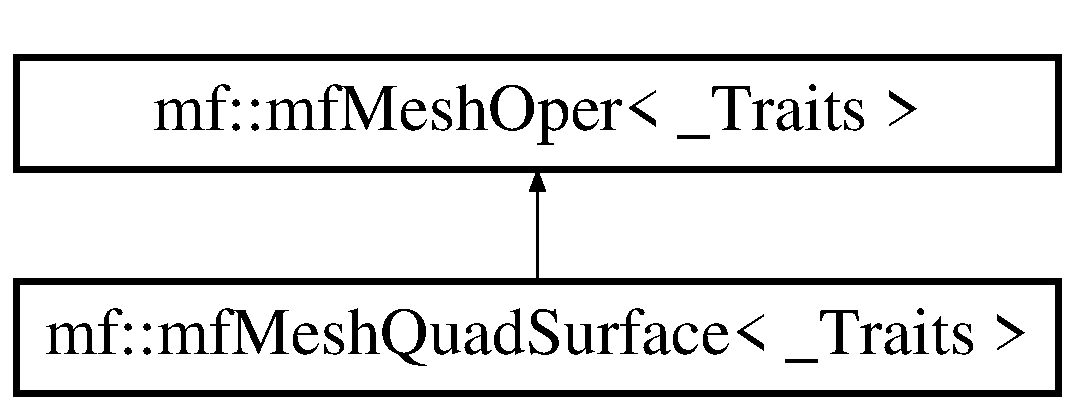
\includegraphics[height=2.000000cm]{classmf_1_1mfMeshQuadSurface}
\end{center}
\end{figure}
\subsection*{Public Types}
\begin{DoxyCompactItemize}
\item 
typedef \_\-Traits::ids \hyperlink{classmf_1_1mfMeshQuadSurface_a91f8c5a330192db329f7b2e116b9149d}{ids}
\item 
typedef \_\-Traits::sVertex \hyperlink{classmf_1_1mfMeshQuadSurface_a2a559debe3d66c95dddb91d4067573a1}{sVertex}
\item 
typedef \_\-Traits::sCell \hyperlink{classmf_1_1mfMeshQuadSurface_a1d1590394548b06c8c8ee3b6a9a7b242}{sCell}
\item 
typedef \hyperlink{classmf_1_1mfSing}{mfSing}$<$ \_\-Traits $>$ \hyperlink{classmf_1_1mfMeshQuadSurface_a416ad67b5e6186e038723e9098472631}{sSing}
\item 
typedef \_\-Traits::sMesh \hyperlink{classmf_1_1mfMeshQuadSurface_a5c71a1c02ec20c5c33393f8bd256168d}{sMesh}
\end{DoxyCompactItemize}
\subsection*{Public Member Functions}
\begin{DoxyCompactItemize}
\item 
\hyperlink{classmf_1_1mfMeshQuadSurface_ada24488577fc8be236ae3bc9c330c8d9}{mfMeshQuadSurface} (\hyperlink{classmf_1_1mfMeshOper_a96c05da9a054cf9ac58d15211922f936}{sMesh} $\ast$\_\-mesh)
\item 
\hyperlink{classmf_1_1mfMeshQuadSurface_ae15089bf425570d5de705ba132711d8b}{$\sim$mfMeshQuadSurface} ()
\item 
void \hyperlink{classmf_1_1mfMeshQuadSurface_af445edf48a12e761d93e91330bc7da99}{addCell} (\hyperlink{classmf_1_1mfMeshOper_a526d1466339244781fbdc0dbfe5ad210}{ids} idcell, \hyperlink{classmf_1_1mfMeshOper_a526d1466339244781fbdc0dbfe5ad210}{ids} $\ast$idvertices MF\_\-DMUTEXVD)
\item 
void \hyperlink{classmf_1_1mfMeshQuadSurface_add51cb72f83e0d0b7afed26e303bad02}{delCell} (\hyperlink{classmf_1_1mfMeshOper_a526d1466339244781fbdc0dbfe5ad210}{ids} idcell MF\_\-DMUTEXVD)
\end{DoxyCompactItemize}
\subsubsection*{template$<$class \_\-Traits$>$ class mf::mfMeshQuadSurface$<$ \_\-Traits $>$}



\subsection{Member Typedef Documentation}
\hypertarget{classmf_1_1mfMeshQuadSurface_a91f8c5a330192db329f7b2e116b9149d}{
\index{mf::mfMeshQuadSurface@{mf::mfMeshQuadSurface}!ids@{ids}}
\index{ids@{ids}!mf::mfMeshQuadSurface@{mf::mfMeshQuadSurface}}
\subsubsection[{ids}]{\setlength{\rightskip}{0pt plus 5cm}template$<$class \_\-Traits $>$ typedef \_\-Traits::ids {\bf mf::mfMeshQuadSurface}$<$ \_\-Traits $>$::{\bf ids}}}
\label{classmf_1_1mfMeshQuadSurface_a91f8c5a330192db329f7b2e116b9149d}
Id typename definition 

Reimplemented from \hyperlink{classmf_1_1mfMeshOper_a526d1466339244781fbdc0dbfe5ad210}{mf::mfMeshOper$<$ \_\-Traits $>$}.

\hypertarget{classmf_1_1mfMeshQuadSurface_a1d1590394548b06c8c8ee3b6a9a7b242}{
\index{mf::mfMeshQuadSurface@{mf::mfMeshQuadSurface}!sCell@{sCell}}
\index{sCell@{sCell}!mf::mfMeshQuadSurface@{mf::mfMeshQuadSurface}}
\subsubsection[{sCell}]{\setlength{\rightskip}{0pt plus 5cm}template$<$class \_\-Traits $>$ typedef \_\-Traits::sCell {\bf mf::mfMeshQuadSurface}$<$ \_\-Traits $>$::{\bf sCell}}}
\label{classmf_1_1mfMeshQuadSurface_a1d1590394548b06c8c8ee3b6a9a7b242}
Cell typename definition \hypertarget{classmf_1_1mfMeshQuadSurface_a5c71a1c02ec20c5c33393f8bd256168d}{
\index{mf::mfMeshQuadSurface@{mf::mfMeshQuadSurface}!sMesh@{sMesh}}
\index{sMesh@{sMesh}!mf::mfMeshQuadSurface@{mf::mfMeshQuadSurface}}
\subsubsection[{sMesh}]{\setlength{\rightskip}{0pt plus 5cm}template$<$class \_\-Traits $>$ typedef \_\-Traits::sMesh {\bf mf::mfMeshQuadSurface}$<$ \_\-Traits $>$::{\bf sMesh}}}
\label{classmf_1_1mfMeshQuadSurface_a5c71a1c02ec20c5c33393f8bd256168d}
/mesh typename definition 

Reimplemented from \hyperlink{classmf_1_1mfMeshOper_a96c05da9a054cf9ac58d15211922f936}{mf::mfMeshOper$<$ \_\-Traits $>$}.

\hypertarget{classmf_1_1mfMeshQuadSurface_a416ad67b5e6186e038723e9098472631}{
\index{mf::mfMeshQuadSurface@{mf::mfMeshQuadSurface}!sSing@{sSing}}
\index{sSing@{sSing}!mf::mfMeshQuadSurface@{mf::mfMeshQuadSurface}}
\subsubsection[{sSing}]{\setlength{\rightskip}{0pt plus 5cm}template$<$class \_\-Traits $>$ typedef {\bf mfSing}$<$\_\-Traits$>$ {\bf mf::mfMeshQuadSurface}$<$ \_\-Traits $>$::{\bf sSing}}}
\label{classmf_1_1mfMeshQuadSurface_a416ad67b5e6186e038723e9098472631}
Singular typename definition \hypertarget{classmf_1_1mfMeshQuadSurface_a2a559debe3d66c95dddb91d4067573a1}{
\index{mf::mfMeshQuadSurface@{mf::mfMeshQuadSurface}!sVertex@{sVertex}}
\index{sVertex@{sVertex}!mf::mfMeshQuadSurface@{mf::mfMeshQuadSurface}}
\subsubsection[{sVertex}]{\setlength{\rightskip}{0pt plus 5cm}template$<$class \_\-Traits $>$ typedef \_\-Traits::sVertex {\bf mf::mfMeshQuadSurface}$<$ \_\-Traits $>$::{\bf sVertex}}}
\label{classmf_1_1mfMeshQuadSurface_a2a559debe3d66c95dddb91d4067573a1}
Vertex typename definition 

\subsection{Constructor \& Destructor Documentation}
\hypertarget{classmf_1_1mfMeshQuadSurface_ada24488577fc8be236ae3bc9c330c8d9}{
\index{mf::mfMeshQuadSurface@{mf::mfMeshQuadSurface}!mfMeshQuadSurface@{mfMeshQuadSurface}}
\index{mfMeshQuadSurface@{mfMeshQuadSurface}!mf::mfMeshQuadSurface@{mf::mfMeshQuadSurface}}
\subsubsection[{mfMeshQuadSurface}]{\setlength{\rightskip}{0pt plus 5cm}template$<$class \_\-Traits $>$ {\bf mf::mfMeshQuadSurface}$<$ \_\-Traits $>$::{\bf mfMeshQuadSurface} (
\begin{DoxyParamCaption}
\item[{{\bf sMesh} $\ast$}]{\_\-mesh}
\end{DoxyParamCaption}
)}}
\label{classmf_1_1mfMeshQuadSurface_ada24488577fc8be236ae3bc9c330c8d9}
Constructor


\begin{DoxyParams}{Parameters}
{\em \_\-mesh,:} & the mesh address that this class will manipulate \\
\hline
\end{DoxyParams}
\hypertarget{classmf_1_1mfMeshQuadSurface_ae15089bf425570d5de705ba132711d8b}{
\index{mf::mfMeshQuadSurface@{mf::mfMeshQuadSurface}!$\sim$mfMeshQuadSurface@{$\sim$mfMeshQuadSurface}}
\index{$\sim$mfMeshQuadSurface@{$\sim$mfMeshQuadSurface}!mf::mfMeshQuadSurface@{mf::mfMeshQuadSurface}}
\subsubsection[{$\sim$mfMeshQuadSurface}]{\setlength{\rightskip}{0pt plus 5cm}template$<$class \_\-Traits $>$ {\bf mf::mfMeshQuadSurface}$<$ \_\-Traits $>$::$\sim${\bf mfMeshQuadSurface} (
\begin{DoxyParamCaption}
{}
\end{DoxyParamCaption}
)}}
\label{classmf_1_1mfMeshQuadSurface_ae15089bf425570d5de705ba132711d8b}
Destructor 

\subsection{Member Function Documentation}
\hypertarget{classmf_1_1mfMeshQuadSurface_af445edf48a12e761d93e91330bc7da99}{
\index{mf::mfMeshQuadSurface@{mf::mfMeshQuadSurface}!addCell@{addCell}}
\index{addCell@{addCell}!mf::mfMeshQuadSurface@{mf::mfMeshQuadSurface}}
\subsubsection[{addCell}]{\setlength{\rightskip}{0pt plus 5cm}template$<$class \_\-Traits $>$ void {\bf mf::mfMeshQuadSurface}$<$ \_\-Traits $>$::addCell (
\begin{DoxyParamCaption}
\item[{{\bf ids}}]{idcell, }
\item[{{\bf ids} $\ast$idvertices}]{MF\_\-DMUTEXVD}
\end{DoxyParamCaption}
)}}
\label{classmf_1_1mfMeshQuadSurface_af445edf48a12e761d93e91330bc7da99}
Add cell in mesh


\begin{DoxyParams}{Parameters}
{\em idcell,:} & cell id \\
\hline
{\em idvertices,:} & vector with vertices ids of the cell \\
\hline
\end{DoxyParams}
\hypertarget{classmf_1_1mfMeshQuadSurface_add51cb72f83e0d0b7afed26e303bad02}{
\index{mf::mfMeshQuadSurface@{mf::mfMeshQuadSurface}!delCell@{delCell}}
\index{delCell@{delCell}!mf::mfMeshQuadSurface@{mf::mfMeshQuadSurface}}
\subsubsection[{delCell}]{\setlength{\rightskip}{0pt plus 5cm}template$<$class \_\-Traits $>$ void {\bf mf::mfMeshQuadSurface}$<$ \_\-Traits $>$::delCell (
\begin{DoxyParamCaption}
\item[{{\bf ids} idcell}]{MF\_\-DMUTEXVD}
\end{DoxyParamCaption}
)}}
\label{classmf_1_1mfMeshQuadSurface_add51cb72f83e0d0b7afed26e303bad02}
Delete a cell


\begin{DoxyParams}{Parameters}
{\em idcell,:} & cell id \\
\hline
\end{DoxyParams}


The documentation for this class was generated from the following file:\begin{DoxyCompactItemize}
\item 
\hyperlink{mfMeshQuadSurface_8h}{mfMeshQuadSurface.h}\end{DoxyCompactItemize}

\hypertarget{classmf_1_1mfMeshTetra}{
\section{mf::mfMeshTetra$<$ \_\-Traits $>$ Class Template Reference}
\label{classmf_1_1mfMeshTetra}\index{mf::mfMeshTetra@{mf::mfMeshTetra}}
}
Inheritance diagram for mf::mfMeshTetra$<$ \_\-Traits $>$:\begin{figure}[H]
\begin{center}
\leavevmode
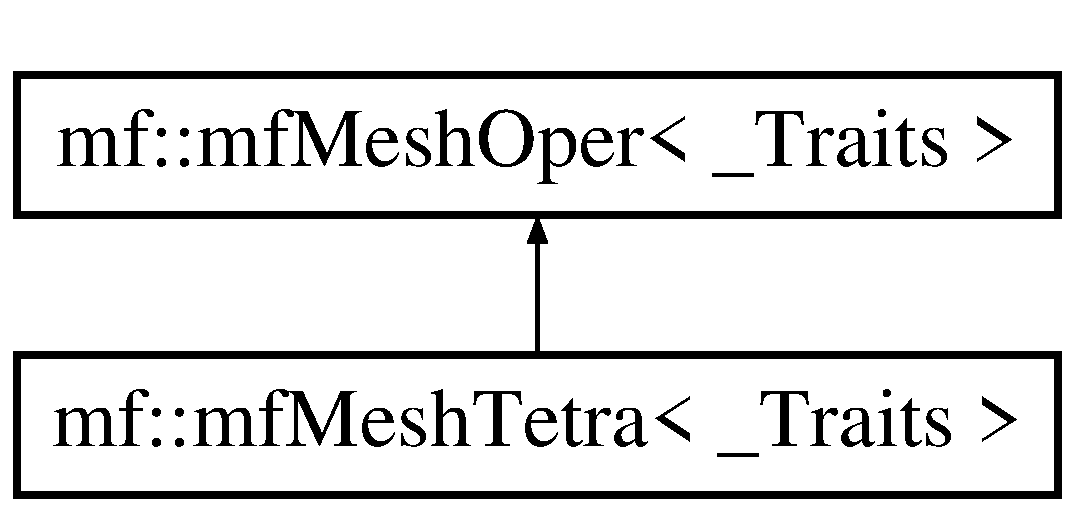
\includegraphics[height=2.000000cm]{classmf_1_1mfMeshTetra}
\end{center}
\end{figure}
\subsection*{Public Types}
\begin{DoxyCompactItemize}
\item 
typedef \_\-Traits::ids \hyperlink{classmf_1_1mfMeshTetra_adbcfde79b2f9076ed56ea0e373508967}{ids}
\item 
typedef \_\-Traits::sVertex \hyperlink{classmf_1_1mfMeshTetra_af6163ef8da6cda46de096af87fd82a55}{sVertex}
\item 
typedef \_\-Traits::sCell \hyperlink{classmf_1_1mfMeshTetra_a3d0b16a5e1666b21e408c3f2e6beac3d}{sCell}
\item 
typedef \_\-Traits::sGeometric \hyperlink{classmf_1_1mfMeshTetra_aebc07dc4fa46c943b52b4fead1a7927c}{sGeometric}
\item 
typedef \hyperlink{classmf_1_1mfSing}{mfSing}$<$ \_\-Traits $>$ \hyperlink{classmf_1_1mfMeshTetra_a85faa5c67167ee9364e5940f320a2693}{sSing}
\item 
typedef \_\-Traits::sMesh \hyperlink{classmf_1_1mfMeshTetra_a1b1ccf8633127e7307c35b150a522193}{sMesh}
\end{DoxyCompactItemize}
\subsection*{Public Member Functions}
\begin{DoxyCompactItemize}
\item 
\hyperlink{classmf_1_1mfMeshTetra_ad12f5ae64d785b5af6bd2753f4326ed9}{mfMeshTetra} (\hyperlink{classmf_1_1mfMeshOper_a96c05da9a054cf9ac58d15211922f936}{sMesh} $\ast$\_\-mesh)
\item 
\hyperlink{classmf_1_1mfMeshTetra_a20f8cd32b95463e348cd41a0a47e543f}{$\sim$mfMeshTetra} ()
\item 
void \hyperlink{classmf_1_1mfMeshTetra_a632bfd4a2844c8df3f3d40752fc6f72b}{addCell} (\hyperlink{classmf_1_1mfMeshOper_a526d1466339244781fbdc0dbfe5ad210}{ids} idcell, \hyperlink{classmf_1_1mfMeshOper_a526d1466339244781fbdc0dbfe5ad210}{ids} $\ast$idvertices MF\_\-DMUTEXVD)
\item 
void \hyperlink{classmf_1_1mfMeshTetra_af77ff3cb397cb9aca88e58004519e5f8}{delCell} (\hyperlink{classmf_1_1mfMeshOper_a526d1466339244781fbdc0dbfe5ad210}{ids} idcell MF\_\-DMUTEXVD)
\end{DoxyCompactItemize}
\subsubsection*{template$<$class \_\-Traits$>$ class mf::mfMeshTetra$<$ \_\-Traits $>$}



\subsection{Member Typedef Documentation}
\hypertarget{classmf_1_1mfMeshTetra_adbcfde79b2f9076ed56ea0e373508967}{
\index{mf::mfMeshTetra@{mf::mfMeshTetra}!ids@{ids}}
\index{ids@{ids}!mf::mfMeshTetra@{mf::mfMeshTetra}}
\subsubsection[{ids}]{\setlength{\rightskip}{0pt plus 5cm}template$<$class \_\-Traits $>$ typedef \_\-Traits::ids {\bf mf::mfMeshTetra}$<$ \_\-Traits $>$::{\bf ids}}}
\label{classmf_1_1mfMeshTetra_adbcfde79b2f9076ed56ea0e373508967}
Id typename definition 

Reimplemented from \hyperlink{classmf_1_1mfMeshOper_a526d1466339244781fbdc0dbfe5ad210}{mf::mfMeshOper$<$ \_\-Traits $>$}.

\hypertarget{classmf_1_1mfMeshTetra_a3d0b16a5e1666b21e408c3f2e6beac3d}{
\index{mf::mfMeshTetra@{mf::mfMeshTetra}!sCell@{sCell}}
\index{sCell@{sCell}!mf::mfMeshTetra@{mf::mfMeshTetra}}
\subsubsection[{sCell}]{\setlength{\rightskip}{0pt plus 5cm}template$<$class \_\-Traits $>$ typedef \_\-Traits::sCell {\bf mf::mfMeshTetra}$<$ \_\-Traits $>$::{\bf sCell}}}
\label{classmf_1_1mfMeshTetra_a3d0b16a5e1666b21e408c3f2e6beac3d}
Cell typename definition \hypertarget{classmf_1_1mfMeshTetra_aebc07dc4fa46c943b52b4fead1a7927c}{
\index{mf::mfMeshTetra@{mf::mfMeshTetra}!sGeometric@{sGeometric}}
\index{sGeometric@{sGeometric}!mf::mfMeshTetra@{mf::mfMeshTetra}}
\subsubsection[{sGeometric}]{\setlength{\rightskip}{0pt plus 5cm}template$<$class \_\-Traits $>$ typedef \_\-Traits::sGeometric {\bf mf::mfMeshTetra}$<$ \_\-Traits $>$::{\bf sGeometric}}}
\label{classmf_1_1mfMeshTetra_aebc07dc4fa46c943b52b4fead1a7927c}
Geometric operator typename definition \hypertarget{classmf_1_1mfMeshTetra_a1b1ccf8633127e7307c35b150a522193}{
\index{mf::mfMeshTetra@{mf::mfMeshTetra}!sMesh@{sMesh}}
\index{sMesh@{sMesh}!mf::mfMeshTetra@{mf::mfMeshTetra}}
\subsubsection[{sMesh}]{\setlength{\rightskip}{0pt plus 5cm}template$<$class \_\-Traits $>$ typedef \_\-Traits::sMesh {\bf mf::mfMeshTetra}$<$ \_\-Traits $>$::{\bf sMesh}}}
\label{classmf_1_1mfMeshTetra_a1b1ccf8633127e7307c35b150a522193}
Mesh typename definition 

Reimplemented from \hyperlink{classmf_1_1mfMeshOper_a96c05da9a054cf9ac58d15211922f936}{mf::mfMeshOper$<$ \_\-Traits $>$}.

\hypertarget{classmf_1_1mfMeshTetra_a85faa5c67167ee9364e5940f320a2693}{
\index{mf::mfMeshTetra@{mf::mfMeshTetra}!sSing@{sSing}}
\index{sSing@{sSing}!mf::mfMeshTetra@{mf::mfMeshTetra}}
\subsubsection[{sSing}]{\setlength{\rightskip}{0pt plus 5cm}template$<$class \_\-Traits $>$ typedef {\bf mfSing}$<$\_\-Traits$>$ {\bf mf::mfMeshTetra}$<$ \_\-Traits $>$::{\bf sSing}}}
\label{classmf_1_1mfMeshTetra_a85faa5c67167ee9364e5940f320a2693}
Singular typename definition \hypertarget{classmf_1_1mfMeshTetra_af6163ef8da6cda46de096af87fd82a55}{
\index{mf::mfMeshTetra@{mf::mfMeshTetra}!sVertex@{sVertex}}
\index{sVertex@{sVertex}!mf::mfMeshTetra@{mf::mfMeshTetra}}
\subsubsection[{sVertex}]{\setlength{\rightskip}{0pt plus 5cm}template$<$class \_\-Traits $>$ typedef \_\-Traits::sVertex {\bf mf::mfMeshTetra}$<$ \_\-Traits $>$::{\bf sVertex}}}
\label{classmf_1_1mfMeshTetra_af6163ef8da6cda46de096af87fd82a55}
Vertex typename definition 

\subsection{Constructor \& Destructor Documentation}
\hypertarget{classmf_1_1mfMeshTetra_ad12f5ae64d785b5af6bd2753f4326ed9}{
\index{mf::mfMeshTetra@{mf::mfMeshTetra}!mfMeshTetra@{mfMeshTetra}}
\index{mfMeshTetra@{mfMeshTetra}!mf::mfMeshTetra@{mf::mfMeshTetra}}
\subsubsection[{mfMeshTetra}]{\setlength{\rightskip}{0pt plus 5cm}template$<$class \_\-Traits $>$ {\bf mf::mfMeshTetra}$<$ \_\-Traits $>$::{\bf mfMeshTetra} (
\begin{DoxyParamCaption}
\item[{{\bf sMesh} $\ast$}]{\_\-mesh}
\end{DoxyParamCaption}
)}}
\label{classmf_1_1mfMeshTetra_ad12f5ae64d785b5af6bd2753f4326ed9}
Constructor


\begin{DoxyParams}{Parameters}
{\em \_\-mesh,:} & the mesh address that this class will manipulate \\
\hline
\end{DoxyParams}
\hypertarget{classmf_1_1mfMeshTetra_a20f8cd32b95463e348cd41a0a47e543f}{
\index{mf::mfMeshTetra@{mf::mfMeshTetra}!$\sim$mfMeshTetra@{$\sim$mfMeshTetra}}
\index{$\sim$mfMeshTetra@{$\sim$mfMeshTetra}!mf::mfMeshTetra@{mf::mfMeshTetra}}
\subsubsection[{$\sim$mfMeshTetra}]{\setlength{\rightskip}{0pt plus 5cm}template$<$class \_\-Traits $>$ {\bf mf::mfMeshTetra}$<$ \_\-Traits $>$::$\sim${\bf mfMeshTetra} (
\begin{DoxyParamCaption}
{}
\end{DoxyParamCaption}
)}}
\label{classmf_1_1mfMeshTetra_a20f8cd32b95463e348cd41a0a47e543f}
Destructor 

\subsection{Member Function Documentation}
\hypertarget{classmf_1_1mfMeshTetra_a632bfd4a2844c8df3f3d40752fc6f72b}{
\index{mf::mfMeshTetra@{mf::mfMeshTetra}!addCell@{addCell}}
\index{addCell@{addCell}!mf::mfMeshTetra@{mf::mfMeshTetra}}
\subsubsection[{addCell}]{\setlength{\rightskip}{0pt plus 5cm}template$<$class \_\-Traits $>$ void {\bf mf::mfMeshTetra}$<$ \_\-Traits $>$::addCell (
\begin{DoxyParamCaption}
\item[{{\bf ids}}]{idcell, }
\item[{{\bf ids} $\ast$idvertices}]{MF\_\-DMUTEXVD}
\end{DoxyParamCaption}
)}}
\label{classmf_1_1mfMeshTetra_a632bfd4a2844c8df3f3d40752fc6f72b}
Add cell in mesh


\begin{DoxyParams}{Parameters}
{\em idcell,:} & cell id \\
\hline
{\em idvertices,:} & vector with vertices ids of the cell \\
\hline
\end{DoxyParams}
\hypertarget{classmf_1_1mfMeshTetra_af77ff3cb397cb9aca88e58004519e5f8}{
\index{mf::mfMeshTetra@{mf::mfMeshTetra}!delCell@{delCell}}
\index{delCell@{delCell}!mf::mfMeshTetra@{mf::mfMeshTetra}}
\subsubsection[{delCell}]{\setlength{\rightskip}{0pt plus 5cm}template$<$class \_\-Traits $>$ void {\bf mf::mfMeshTetra}$<$ \_\-Traits $>$::delCell (
\begin{DoxyParamCaption}
\item[{{\bf ids} idcell}]{MF\_\-DMUTEXVD}
\end{DoxyParamCaption}
)}}
\label{classmf_1_1mfMeshTetra_af77ff3cb397cb9aca88e58004519e5f8}
Delete a cell


\begin{DoxyParams}{Parameters}
{\em idcell,:} & cell id \\
\hline
\end{DoxyParams}


The documentation for this class was generated from the following file:\begin{DoxyCompactItemize}
\item 
\hyperlink{mfMeshTetra_8h}{mfMeshTetra.h}\end{DoxyCompactItemize}

\hypertarget{classmf_1_1mfMeshTriSurface}{
\section{mf::mfMeshTriSurface$<$ \_\-Traits $>$ Class Template Reference}
\label{classmf_1_1mfMeshTriSurface}\index{mf::mfMeshTriSurface@{mf::mfMeshTriSurface}}
}
Inheritance diagram for mf::mfMeshTriSurface$<$ \_\-Traits $>$:\begin{figure}[H]
\begin{center}
\leavevmode
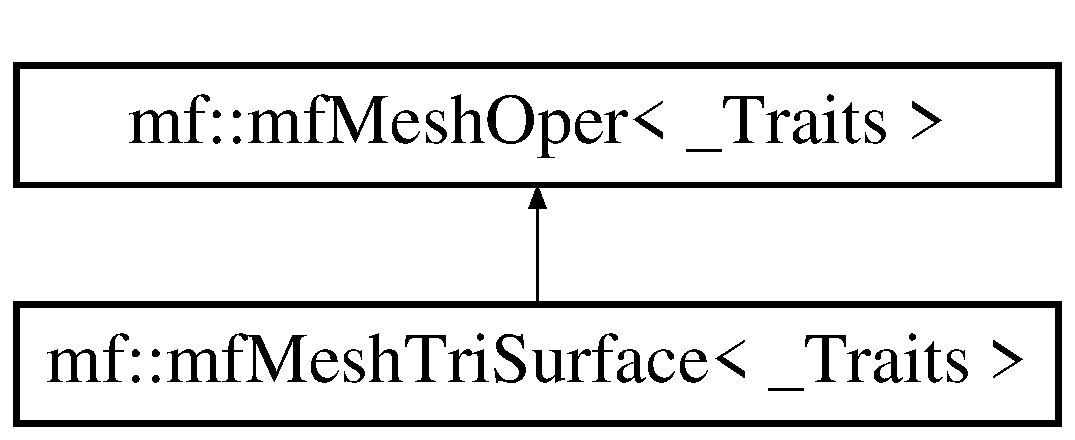
\includegraphics[height=2.000000cm]{classmf_1_1mfMeshTriSurface}
\end{center}
\end{figure}
\subsection*{Public Types}
\begin{DoxyCompactItemize}
\item 
typedef \_\-Traits::ids \hyperlink{classmf_1_1mfMeshTriSurface_a2432b4eb1b385605e96d17e2774519f5}{ids}
\item 
typedef \_\-Traits::sVertex \hyperlink{classmf_1_1mfMeshTriSurface_a2408391103a6d2805d76654edd468059}{sVertex}
\item 
typedef \_\-Traits::sCell \hyperlink{classmf_1_1mfMeshTriSurface_a75283f44a5903a67f6bbb7094b8a900f}{sCell}
\item 
typedef \hyperlink{classmf_1_1mfSing}{mfSing}$<$ \_\-Traits $>$ \hyperlink{classmf_1_1mfMeshTriSurface_ae3b4bcef281c3802394aa264db8bcfa8}{sSing}
\item 
typedef \_\-Traits::sMesh \hyperlink{classmf_1_1mfMeshTriSurface_aa25d8c016f15b0073c5ba5aa0a64be86}{sMesh}
\end{DoxyCompactItemize}
\subsection*{Public Member Functions}
\begin{DoxyCompactItemize}
\item 
\hyperlink{classmf_1_1mfMeshTriSurface_a65c2be08d78df0b8730f242c3ab1c30c}{mfMeshTriSurface} (\hyperlink{classmf_1_1mfMeshOper_a96c05da9a054cf9ac58d15211922f936}{sMesh} $\ast$\_\-mesh)
\item 
\hyperlink{classmf_1_1mfMeshTriSurface_ab9d17a264650f0cd52308e7b07580b5a}{$\sim$mfMeshTriSurface} ()
\item 
void \hyperlink{classmf_1_1mfMeshTriSurface_afde5244f145f55c02da44551007a4714}{addCell} (\hyperlink{classmf_1_1mfMeshOper_a526d1466339244781fbdc0dbfe5ad210}{ids} idcell, \hyperlink{classmf_1_1mfMeshOper_a526d1466339244781fbdc0dbfe5ad210}{ids} $\ast$idvertices MF\_\-DMUTEXVD)
\item 
void \hyperlink{classmf_1_1mfMeshTriSurface_a355433359c4c4137b1f1a271278a7cbe}{delCell} (\hyperlink{classmf_1_1mfMeshOper_a526d1466339244781fbdc0dbfe5ad210}{ids} idcell MF\_\-DMUTEXVD)
\end{DoxyCompactItemize}
\subsubsection*{template$<$class \_\-Traits$>$ class mf::mfMeshTriSurface$<$ \_\-Traits $>$}



\subsection{Member Typedef Documentation}
\hypertarget{classmf_1_1mfMeshTriSurface_a2432b4eb1b385605e96d17e2774519f5}{
\index{mf::mfMeshTriSurface@{mf::mfMeshTriSurface}!ids@{ids}}
\index{ids@{ids}!mf::mfMeshTriSurface@{mf::mfMeshTriSurface}}
\subsubsection[{ids}]{\setlength{\rightskip}{0pt plus 5cm}template$<$class \_\-Traits $>$ typedef \_\-Traits::ids {\bf mf::mfMeshTriSurface}$<$ \_\-Traits $>$::{\bf ids}}}
\label{classmf_1_1mfMeshTriSurface_a2432b4eb1b385605e96d17e2774519f5}
Id typename definition 

Reimplemented from \hyperlink{classmf_1_1mfMeshOper_a526d1466339244781fbdc0dbfe5ad210}{mf::mfMeshOper$<$ \_\-Traits $>$}.

\hypertarget{classmf_1_1mfMeshTriSurface_a75283f44a5903a67f6bbb7094b8a900f}{
\index{mf::mfMeshTriSurface@{mf::mfMeshTriSurface}!sCell@{sCell}}
\index{sCell@{sCell}!mf::mfMeshTriSurface@{mf::mfMeshTriSurface}}
\subsubsection[{sCell}]{\setlength{\rightskip}{0pt plus 5cm}template$<$class \_\-Traits $>$ typedef \_\-Traits::sCell {\bf mf::mfMeshTriSurface}$<$ \_\-Traits $>$::{\bf sCell}}}
\label{classmf_1_1mfMeshTriSurface_a75283f44a5903a67f6bbb7094b8a900f}
Cell typename definition \hypertarget{classmf_1_1mfMeshTriSurface_aa25d8c016f15b0073c5ba5aa0a64be86}{
\index{mf::mfMeshTriSurface@{mf::mfMeshTriSurface}!sMesh@{sMesh}}
\index{sMesh@{sMesh}!mf::mfMeshTriSurface@{mf::mfMeshTriSurface}}
\subsubsection[{sMesh}]{\setlength{\rightskip}{0pt plus 5cm}template$<$class \_\-Traits $>$ typedef \_\-Traits::sMesh {\bf mf::mfMeshTriSurface}$<$ \_\-Traits $>$::{\bf sMesh}}}
\label{classmf_1_1mfMeshTriSurface_aa25d8c016f15b0073c5ba5aa0a64be86}
Mesh typename definition 

Reimplemented from \hyperlink{classmf_1_1mfMeshOper_a96c05da9a054cf9ac58d15211922f936}{mf::mfMeshOper$<$ \_\-Traits $>$}.

\hypertarget{classmf_1_1mfMeshTriSurface_ae3b4bcef281c3802394aa264db8bcfa8}{
\index{mf::mfMeshTriSurface@{mf::mfMeshTriSurface}!sSing@{sSing}}
\index{sSing@{sSing}!mf::mfMeshTriSurface@{mf::mfMeshTriSurface}}
\subsubsection[{sSing}]{\setlength{\rightskip}{0pt plus 5cm}template$<$class \_\-Traits $>$ typedef {\bf mfSing}$<$\_\-Traits$>$ {\bf mf::mfMeshTriSurface}$<$ \_\-Traits $>$::{\bf sSing}}}
\label{classmf_1_1mfMeshTriSurface_ae3b4bcef281c3802394aa264db8bcfa8}
Singular typename definition \hypertarget{classmf_1_1mfMeshTriSurface_a2408391103a6d2805d76654edd468059}{
\index{mf::mfMeshTriSurface@{mf::mfMeshTriSurface}!sVertex@{sVertex}}
\index{sVertex@{sVertex}!mf::mfMeshTriSurface@{mf::mfMeshTriSurface}}
\subsubsection[{sVertex}]{\setlength{\rightskip}{0pt plus 5cm}template$<$class \_\-Traits $>$ typedef \_\-Traits::sVertex {\bf mf::mfMeshTriSurface}$<$ \_\-Traits $>$::{\bf sVertex}}}
\label{classmf_1_1mfMeshTriSurface_a2408391103a6d2805d76654edd468059}
Vertex typename definition 

\subsection{Constructor \& Destructor Documentation}
\hypertarget{classmf_1_1mfMeshTriSurface_a65c2be08d78df0b8730f242c3ab1c30c}{
\index{mf::mfMeshTriSurface@{mf::mfMeshTriSurface}!mfMeshTriSurface@{mfMeshTriSurface}}
\index{mfMeshTriSurface@{mfMeshTriSurface}!mf::mfMeshTriSurface@{mf::mfMeshTriSurface}}
\subsubsection[{mfMeshTriSurface}]{\setlength{\rightskip}{0pt plus 5cm}template$<$class \_\-Traits $>$ {\bf mf::mfMeshTriSurface}$<$ \_\-Traits $>$::{\bf mfMeshTriSurface} (
\begin{DoxyParamCaption}
\item[{{\bf sMesh} $\ast$}]{\_\-mesh}
\end{DoxyParamCaption}
)}}
\label{classmf_1_1mfMeshTriSurface_a65c2be08d78df0b8730f242c3ab1c30c}
Constructor


\begin{DoxyParams}{Parameters}
{\em \_\-mesh,:} & the mesh address that this class will manipulate \\
\hline
\end{DoxyParams}
\hypertarget{classmf_1_1mfMeshTriSurface_ab9d17a264650f0cd52308e7b07580b5a}{
\index{mf::mfMeshTriSurface@{mf::mfMeshTriSurface}!$\sim$mfMeshTriSurface@{$\sim$mfMeshTriSurface}}
\index{$\sim$mfMeshTriSurface@{$\sim$mfMeshTriSurface}!mf::mfMeshTriSurface@{mf::mfMeshTriSurface}}
\subsubsection[{$\sim$mfMeshTriSurface}]{\setlength{\rightskip}{0pt plus 5cm}template$<$class \_\-Traits $>$ {\bf mf::mfMeshTriSurface}$<$ \_\-Traits $>$::$\sim${\bf mfMeshTriSurface} (
\begin{DoxyParamCaption}
{}
\end{DoxyParamCaption}
)}}
\label{classmf_1_1mfMeshTriSurface_ab9d17a264650f0cd52308e7b07580b5a}
Destructor 

\subsection{Member Function Documentation}
\hypertarget{classmf_1_1mfMeshTriSurface_afde5244f145f55c02da44551007a4714}{
\index{mf::mfMeshTriSurface@{mf::mfMeshTriSurface}!addCell@{addCell}}
\index{addCell@{addCell}!mf::mfMeshTriSurface@{mf::mfMeshTriSurface}}
\subsubsection[{addCell}]{\setlength{\rightskip}{0pt plus 5cm}template$<$class \_\-Traits $>$ void {\bf mf::mfMeshTriSurface}$<$ \_\-Traits $>$::addCell (
\begin{DoxyParamCaption}
\item[{{\bf ids}}]{idcell, }
\item[{{\bf ids} $\ast$idvertices}]{MF\_\-DMUTEXVD}
\end{DoxyParamCaption}
)}}
\label{classmf_1_1mfMeshTriSurface_afde5244f145f55c02da44551007a4714}
Add cell in mesh


\begin{DoxyParams}{Parameters}
{\em idcell,:} & cell id \\
\hline
{\em idvertices,:} & vector with vertices ids of the cell \\
\hline
\end{DoxyParams}
\hypertarget{classmf_1_1mfMeshTriSurface_a355433359c4c4137b1f1a271278a7cbe}{
\index{mf::mfMeshTriSurface@{mf::mfMeshTriSurface}!delCell@{delCell}}
\index{delCell@{delCell}!mf::mfMeshTriSurface@{mf::mfMeshTriSurface}}
\subsubsection[{delCell}]{\setlength{\rightskip}{0pt plus 5cm}template$<$class \_\-Traits $>$ void {\bf mf::mfMeshTriSurface}$<$ \_\-Traits $>$::delCell (
\begin{DoxyParamCaption}
\item[{{\bf ids} idcell}]{MF\_\-DMUTEXVD}
\end{DoxyParamCaption}
)}}
\label{classmf_1_1mfMeshTriSurface_a355433359c4c4137b1f1a271278a7cbe}
Delete a cell


\begin{DoxyParams}{Parameters}
{\em idcell,:} & cell id \\
\hline
\end{DoxyParams}


The documentation for this class was generated from the following file:\begin{DoxyCompactItemize}
\item 
\hyperlink{mfMeshTriSurface_8h}{mfMeshTriSurface.h}\end{DoxyCompactItemize}

\hypertarget{classmf_1_1mfMfReader}{
\section{mf::mfMfReader$<$ \_\-Traits $>$ Class Template Reference}
\label{classmf_1_1mfMfReader}\index{mf::mfMfReader@{mf::mfMfReader}}
}
Inheritance diagram for mf::mfMfReader$<$ \_\-Traits $>$:\begin{figure}[H]
\begin{center}
\leavevmode
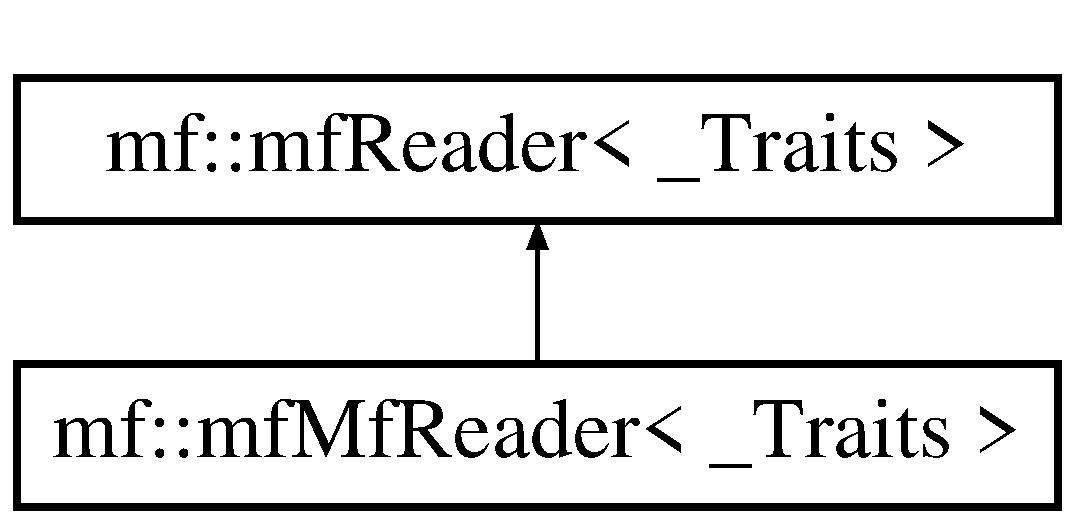
\includegraphics[height=2.000000cm]{classmf_1_1mfMfReader}
\end{center}
\end{figure}
\subsection*{Public Types}
\begin{DoxyCompactItemize}
\item 
typedef \_\-Traits::space \hyperlink{classmf_1_1mfMfReader_afc7cecbd97bfb29aaa9725b37e1e3de6}{space}
\item 
typedef \_\-Traits::ids \hyperlink{classmf_1_1mfMfReader_ace0c24e773b00ea08ddc459d747f4b0b}{ids}
\item 
typedef \_\-Traits::sVertex \hyperlink{classmf_1_1mfMfReader_ae5f152e9da9821af7369d310237c7906}{sVertex}
\item 
typedef \_\-Traits::sCell \hyperlink{classmf_1_1mfMfReader_ad706d4b18bc925ccb011c9973c108dc9}{sCell}
\item 
typedef \_\-Traits::sMesh \hyperlink{classmf_1_1mfMfReader_a12c6ee10508f5805b2cddc729407a1f3}{sMesh}
\item 
typedef \hyperlink{classmf_1_1mfBinaryIO}{mfBinaryIO}$<$ \_\-Traits $>$ \hyperlink{classmf_1_1mfMfReader_a2709026b1c067b6d0e14ed23fdb23a2d}{sBinaryIO}
\end{DoxyCompactItemize}
\subsection*{Public Member Functions}
\begin{DoxyCompactItemize}
\item 
\hyperlink{classmf_1_1mfMfReader_af06cbc1264cf7fbe21bdb43b5dab41e7}{mfMfReader} ()
\item 
\hyperlink{classmf_1_1mfMfReader_a41dce1f0e6bb72b87778bd238966e76a}{$\sim$mfMfReader} ()
\item 
virtual bool \hyperlink{classmf_1_1mfMfReader_a9e43439ba77d2afb25839f3ed4fb774f}{read} (\hyperlink{classmf_1_1mfMfReader_a12c6ee10508f5805b2cddc729407a1f3}{sMesh} $\ast$malha, const char $\ast$filename)
\begin{DoxyCompactList}\small\item\em Executa a leitura de um arquivo. \item\end{DoxyCompactList}\end{DoxyCompactItemize}
\subsubsection*{template$<$class \_\-Traits$>$ class mf::mfMfReader$<$ \_\-Traits $>$}



\subsection{Member Typedef Documentation}
\hypertarget{classmf_1_1mfMfReader_ace0c24e773b00ea08ddc459d747f4b0b}{
\index{mf::mfMfReader@{mf::mfMfReader}!ids@{ids}}
\index{ids@{ids}!mf::mfMfReader@{mf::mfMfReader}}
\subsubsection[{ids}]{\setlength{\rightskip}{0pt plus 5cm}template$<$class \_\-Traits $>$ typedef \_\-Traits::ids {\bf mf::mfMfReader}$<$ \_\-Traits $>$::{\bf ids}}}
\label{classmf_1_1mfMfReader_ace0c24e773b00ea08ddc459d747f4b0b}
Id typename definition \hypertarget{classmf_1_1mfMfReader_a2709026b1c067b6d0e14ed23fdb23a2d}{
\index{mf::mfMfReader@{mf::mfMfReader}!sBinaryIO@{sBinaryIO}}
\index{sBinaryIO@{sBinaryIO}!mf::mfMfReader@{mf::mfMfReader}}
\subsubsection[{sBinaryIO}]{\setlength{\rightskip}{0pt plus 5cm}template$<$class \_\-Traits $>$ typedef {\bf mfBinaryIO}$<$\_\-Traits$>$ {\bf mf::mfMfReader}$<$ \_\-Traits $>$::{\bf sBinaryIO}}}
\label{classmf_1_1mfMfReader_a2709026b1c067b6d0e14ed23fdb23a2d}
Binary in/out typename definition \hypertarget{classmf_1_1mfMfReader_ad706d4b18bc925ccb011c9973c108dc9}{
\index{mf::mfMfReader@{mf::mfMfReader}!sCell@{sCell}}
\index{sCell@{sCell}!mf::mfMfReader@{mf::mfMfReader}}
\subsubsection[{sCell}]{\setlength{\rightskip}{0pt plus 5cm}template$<$class \_\-Traits $>$ typedef \_\-Traits::sCell {\bf mf::mfMfReader}$<$ \_\-Traits $>$::{\bf sCell}}}
\label{classmf_1_1mfMfReader_ad706d4b18bc925ccb011c9973c108dc9}
Cell typename definition \hypertarget{classmf_1_1mfMfReader_a12c6ee10508f5805b2cddc729407a1f3}{
\index{mf::mfMfReader@{mf::mfMfReader}!sMesh@{sMesh}}
\index{sMesh@{sMesh}!mf::mfMfReader@{mf::mfMfReader}}
\subsubsection[{sMesh}]{\setlength{\rightskip}{0pt plus 5cm}template$<$class \_\-Traits $>$ typedef \_\-Traits::sMesh {\bf mf::mfMfReader}$<$ \_\-Traits $>$::{\bf sMesh}}}
\label{classmf_1_1mfMfReader_a12c6ee10508f5805b2cddc729407a1f3}
Mesh typename definition 

Reimplemented from \hyperlink{classmf_1_1mfReader}{mf::mfReader$<$ \_\-Traits $>$}.

\hypertarget{classmf_1_1mfMfReader_afc7cecbd97bfb29aaa9725b37e1e3de6}{
\index{mf::mfMfReader@{mf::mfMfReader}!space@{space}}
\index{space@{space}!mf::mfMfReader@{mf::mfMfReader}}
\subsubsection[{space}]{\setlength{\rightskip}{0pt plus 5cm}template$<$class \_\-Traits $>$ typedef \_\-Traits::space {\bf mf::mfMfReader}$<$ \_\-Traits $>$::{\bf space}}}
\label{classmf_1_1mfMfReader_afc7cecbd97bfb29aaa9725b37e1e3de6}
Space typename definition \hypertarget{classmf_1_1mfMfReader_ae5f152e9da9821af7369d310237c7906}{
\index{mf::mfMfReader@{mf::mfMfReader}!sVertex@{sVertex}}
\index{sVertex@{sVertex}!mf::mfMfReader@{mf::mfMfReader}}
\subsubsection[{sVertex}]{\setlength{\rightskip}{0pt plus 5cm}template$<$class \_\-Traits $>$ typedef \_\-Traits::sVertex {\bf mf::mfMfReader}$<$ \_\-Traits $>$::{\bf sVertex}}}
\label{classmf_1_1mfMfReader_ae5f152e9da9821af7369d310237c7906}
Vertex typename definition 

\subsection{Constructor \& Destructor Documentation}
\hypertarget{classmf_1_1mfMfReader_af06cbc1264cf7fbe21bdb43b5dab41e7}{
\index{mf::mfMfReader@{mf::mfMfReader}!mfMfReader@{mfMfReader}}
\index{mfMfReader@{mfMfReader}!mf::mfMfReader@{mf::mfMfReader}}
\subsubsection[{mfMfReader}]{\setlength{\rightskip}{0pt plus 5cm}template$<$class \_\-Traits $>$ {\bf mf::mfMfReader}$<$ \_\-Traits $>$::{\bf mfMfReader} (
\begin{DoxyParamCaption}
{}
\end{DoxyParamCaption}
)}}
\label{classmf_1_1mfMfReader_af06cbc1264cf7fbe21bdb43b5dab41e7}
Constructor \hypertarget{classmf_1_1mfMfReader_a41dce1f0e6bb72b87778bd238966e76a}{
\index{mf::mfMfReader@{mf::mfMfReader}!$\sim$mfMfReader@{$\sim$mfMfReader}}
\index{$\sim$mfMfReader@{$\sim$mfMfReader}!mf::mfMfReader@{mf::mfMfReader}}
\subsubsection[{$\sim$mfMfReader}]{\setlength{\rightskip}{0pt plus 5cm}template$<$class \_\-Traits $>$ {\bf mf::mfMfReader}$<$ \_\-Traits $>$::$\sim${\bf mfMfReader} (
\begin{DoxyParamCaption}
{}
\end{DoxyParamCaption}
)}}
\label{classmf_1_1mfMfReader_a41dce1f0e6bb72b87778bd238966e76a}
Destructor 

\subsection{Member Function Documentation}
\hypertarget{classmf_1_1mfMfReader_a9e43439ba77d2afb25839f3ed4fb774f}{
\index{mf::mfMfReader@{mf::mfMfReader}!read@{read}}
\index{read@{read}!mf::mfMfReader@{mf::mfMfReader}}
\subsubsection[{read}]{\setlength{\rightskip}{0pt plus 5cm}template$<$class \_\-Traits $>$ bool {\bf mf::mfMfReader}$<$ \_\-Traits $>$::read (
\begin{DoxyParamCaption}
\item[{{\bf sMesh} $\ast$}]{malha, }
\item[{const char $\ast$}]{filename}
\end{DoxyParamCaption}
)\hspace{0.3cm}{\ttfamily  \mbox{[}virtual\mbox{]}}}}
\label{classmf_1_1mfMfReader_a9e43439ba77d2afb25839f3ed4fb774f}


Executa a leitura de um arquivo. 

Paraetros de entrada: malha : endereco de memoria de destino da malha a ser carregada. Ja deve estar alocado. filename : nome do arquivo da malha. 

Implements \hyperlink{classmf_1_1mfReader_a0e0c3224a06b06a8fb82be4f0f4a2e00}{mf::mfReader$<$ \_\-Traits $>$}.



The documentation for this class was generated from the following file:\begin{DoxyCompactItemize}
\item 
mfMfReader.h\end{DoxyCompactItemize}

\hypertarget{classmf_1_1mfMfWriter}{
\section{mf::mfMfWriter$<$ \_\-Traits $>$ Class Template Reference}
\label{classmf_1_1mfMfWriter}\index{mf::mfMfWriter@{mf::mfMfWriter}}
}
Inheritance diagram for mf::mfMfWriter$<$ \_\-Traits $>$:\begin{figure}[H]
\begin{center}
\leavevmode
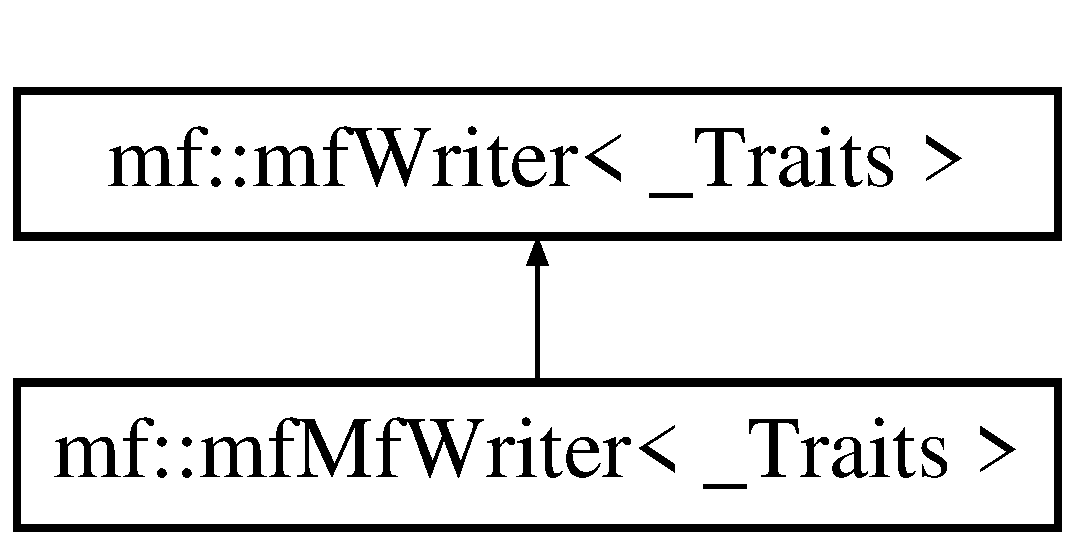
\includegraphics[height=2.000000cm]{classmf_1_1mfMfWriter}
\end{center}
\end{figure}
\subsection*{Public Types}
\begin{DoxyCompactItemize}
\item 
typedef \_\-Traits::space \hyperlink{classmf_1_1mfMfWriter_a21bbac0be4b7669c31b1bb300e21b1e3}{space}
\item 
typedef \_\-Traits::ids \hyperlink{classmf_1_1mfMfWriter_a46296c1b8fe7d05f31495f65457ac945}{ids}
\item 
typedef \_\-Traits::sVertex \hyperlink{classmf_1_1mfMfWriter_a01f8809f4b57ba5f886abe7f511da32c}{sVertex}
\item 
typedef \_\-Traits::sCell \hyperlink{classmf_1_1mfMfWriter_a58fa8a1a76014a24f6f52fc77dd9cbb0}{sCell}
\item 
typedef \_\-Traits::sMesh \hyperlink{classmf_1_1mfMfWriter_a2d08e4dc5186064ec4ef99b2d7442f5c}{sMesh}
\item 
typedef \hyperlink{classmf_1_1mfBinaryIO}{mfBinaryIO}$<$ \_\-Traits $>$ \hyperlink{classmf_1_1mfMfWriter_aeeeccedc6616f608f33cf42ca2e68dcc}{sBinaryIO}
\end{DoxyCompactItemize}
\subsection*{Public Member Functions}
\begin{DoxyCompactItemize}
\item 
\hyperlink{classmf_1_1mfMfWriter_acde356a4e00b8cd677fefedac6e0330b}{mfMfWriter} ()
\item 
\hyperlink{classmf_1_1mfMfWriter_af15ffd11140c3c11ba20496bc12301a9}{$\sim$mfMfWriter} ()
\item 
virtual bool \hyperlink{classmf_1_1mfMfWriter_a2fc75ae58c2e75f24924c812aec7bc8a}{write} (\hyperlink{classmf_1_1mfMfWriter_a2d08e4dc5186064ec4ef99b2d7442f5c}{sMesh} $\ast$malha, const char $\ast$filename)
\begin{DoxyCompactList}\small\item\em Executa a escrita de um arquivo (salva uma malha) \item\end{DoxyCompactList}\end{DoxyCompactItemize}
\subsubsection*{template$<$class \_\-Traits$>$ class mf::mfMfWriter$<$ \_\-Traits $>$}



\subsection{Member Typedef Documentation}
\hypertarget{classmf_1_1mfMfWriter_a46296c1b8fe7d05f31495f65457ac945}{
\index{mf::mfMfWriter@{mf::mfMfWriter}!ids@{ids}}
\index{ids@{ids}!mf::mfMfWriter@{mf::mfMfWriter}}
\subsubsection[{ids}]{\setlength{\rightskip}{0pt plus 5cm}template$<$class \_\-Traits $>$ typedef \_\-Traits::ids {\bf mf::mfMfWriter}$<$ \_\-Traits $>$::{\bf ids}}}
\label{classmf_1_1mfMfWriter_a46296c1b8fe7d05f31495f65457ac945}
Id typename definition \hypertarget{classmf_1_1mfMfWriter_aeeeccedc6616f608f33cf42ca2e68dcc}{
\index{mf::mfMfWriter@{mf::mfMfWriter}!sBinaryIO@{sBinaryIO}}
\index{sBinaryIO@{sBinaryIO}!mf::mfMfWriter@{mf::mfMfWriter}}
\subsubsection[{sBinaryIO}]{\setlength{\rightskip}{0pt plus 5cm}template$<$class \_\-Traits $>$ typedef {\bf mfBinaryIO}$<$\_\-Traits$>$ {\bf mf::mfMfWriter}$<$ \_\-Traits $>$::{\bf sBinaryIO}}}
\label{classmf_1_1mfMfWriter_aeeeccedc6616f608f33cf42ca2e68dcc}
Binary in/out typename definition \hypertarget{classmf_1_1mfMfWriter_a58fa8a1a76014a24f6f52fc77dd9cbb0}{
\index{mf::mfMfWriter@{mf::mfMfWriter}!sCell@{sCell}}
\index{sCell@{sCell}!mf::mfMfWriter@{mf::mfMfWriter}}
\subsubsection[{sCell}]{\setlength{\rightskip}{0pt plus 5cm}template$<$class \_\-Traits $>$ typedef \_\-Traits::sCell {\bf mf::mfMfWriter}$<$ \_\-Traits $>$::{\bf sCell}}}
\label{classmf_1_1mfMfWriter_a58fa8a1a76014a24f6f52fc77dd9cbb0}
Cell typename definition \hypertarget{classmf_1_1mfMfWriter_a2d08e4dc5186064ec4ef99b2d7442f5c}{
\index{mf::mfMfWriter@{mf::mfMfWriter}!sMesh@{sMesh}}
\index{sMesh@{sMesh}!mf::mfMfWriter@{mf::mfMfWriter}}
\subsubsection[{sMesh}]{\setlength{\rightskip}{0pt plus 5cm}template$<$class \_\-Traits $>$ typedef \_\-Traits::sMesh {\bf mf::mfMfWriter}$<$ \_\-Traits $>$::{\bf sMesh}}}
\label{classmf_1_1mfMfWriter_a2d08e4dc5186064ec4ef99b2d7442f5c}
Mesh typename definition 

Reimplemented from \hyperlink{classmf_1_1mfWriter}{mf::mfWriter$<$ \_\-Traits $>$}.

\hypertarget{classmf_1_1mfMfWriter_a21bbac0be4b7669c31b1bb300e21b1e3}{
\index{mf::mfMfWriter@{mf::mfMfWriter}!space@{space}}
\index{space@{space}!mf::mfMfWriter@{mf::mfMfWriter}}
\subsubsection[{space}]{\setlength{\rightskip}{0pt plus 5cm}template$<$class \_\-Traits $>$ typedef \_\-Traits::space {\bf mf::mfMfWriter}$<$ \_\-Traits $>$::{\bf space}}}
\label{classmf_1_1mfMfWriter_a21bbac0be4b7669c31b1bb300e21b1e3}
Space typename definition \hypertarget{classmf_1_1mfMfWriter_a01f8809f4b57ba5f886abe7f511da32c}{
\index{mf::mfMfWriter@{mf::mfMfWriter}!sVertex@{sVertex}}
\index{sVertex@{sVertex}!mf::mfMfWriter@{mf::mfMfWriter}}
\subsubsection[{sVertex}]{\setlength{\rightskip}{0pt plus 5cm}template$<$class \_\-Traits $>$ typedef \_\-Traits::sVertex {\bf mf::mfMfWriter}$<$ \_\-Traits $>$::{\bf sVertex}}}
\label{classmf_1_1mfMfWriter_a01f8809f4b57ba5f886abe7f511da32c}
Vertex typename definition 

\subsection{Constructor \& Destructor Documentation}
\hypertarget{classmf_1_1mfMfWriter_acde356a4e00b8cd677fefedac6e0330b}{
\index{mf::mfMfWriter@{mf::mfMfWriter}!mfMfWriter@{mfMfWriter}}
\index{mfMfWriter@{mfMfWriter}!mf::mfMfWriter@{mf::mfMfWriter}}
\subsubsection[{mfMfWriter}]{\setlength{\rightskip}{0pt plus 5cm}template$<$class \_\-Traits $>$ {\bf mf::mfMfWriter}$<$ \_\-Traits $>$::{\bf mfMfWriter} (
\begin{DoxyParamCaption}
{}
\end{DoxyParamCaption}
)}}
\label{classmf_1_1mfMfWriter_acde356a4e00b8cd677fefedac6e0330b}
Constructor \hypertarget{classmf_1_1mfMfWriter_af15ffd11140c3c11ba20496bc12301a9}{
\index{mf::mfMfWriter@{mf::mfMfWriter}!$\sim$mfMfWriter@{$\sim$mfMfWriter}}
\index{$\sim$mfMfWriter@{$\sim$mfMfWriter}!mf::mfMfWriter@{mf::mfMfWriter}}
\subsubsection[{$\sim$mfMfWriter}]{\setlength{\rightskip}{0pt plus 5cm}template$<$class \_\-Traits $>$ {\bf mf::mfMfWriter}$<$ \_\-Traits $>$::$\sim${\bf mfMfWriter} (
\begin{DoxyParamCaption}
{}
\end{DoxyParamCaption}
)}}
\label{classmf_1_1mfMfWriter_af15ffd11140c3c11ba20496bc12301a9}
Destructor 

\subsection{Member Function Documentation}
\hypertarget{classmf_1_1mfMfWriter_a2fc75ae58c2e75f24924c812aec7bc8a}{
\index{mf::mfMfWriter@{mf::mfMfWriter}!write@{write}}
\index{write@{write}!mf::mfMfWriter@{mf::mfMfWriter}}
\subsubsection[{write}]{\setlength{\rightskip}{0pt plus 5cm}template$<$class \_\-Traits $>$ bool {\bf mf::mfMfWriter}$<$ \_\-Traits $>$::write (
\begin{DoxyParamCaption}
\item[{{\bf sMesh} $\ast$}]{malha, }
\item[{const char $\ast$}]{filename}
\end{DoxyParamCaption}
)\hspace{0.3cm}{\ttfamily  \mbox{[}virtual\mbox{]}}}}
\label{classmf_1_1mfMfWriter_a2fc75ae58c2e75f24924c812aec7bc8a}


Executa a escrita de um arquivo (salva uma malha) 

Paraetros de entrada: malha : endereco de memoria da malha a ser salva. filename : nome do arquivo da malha. (destino) 

Implements \hyperlink{classmf_1_1mfWriter_a85d6c59bdb8fec69222e4157c299256c}{mf::mfWriter$<$ \_\-Traits $>$}.



The documentation for this class was generated from the following file:\begin{DoxyCompactItemize}
\item 
mfMfWriter.h\end{DoxyCompactItemize}

\hypertarget{classmf_1_1mfOffReader}{
\section{mf::mfOffReader$<$ \_\-Traits $>$ Class Template Reference}
\label{classmf_1_1mfOffReader}\index{mf::mfOffReader@{mf::mfOffReader}}
}
Inheritance diagram for mf::mfOffReader$<$ \_\-Traits $>$:\begin{figure}[H]
\begin{center}
\leavevmode
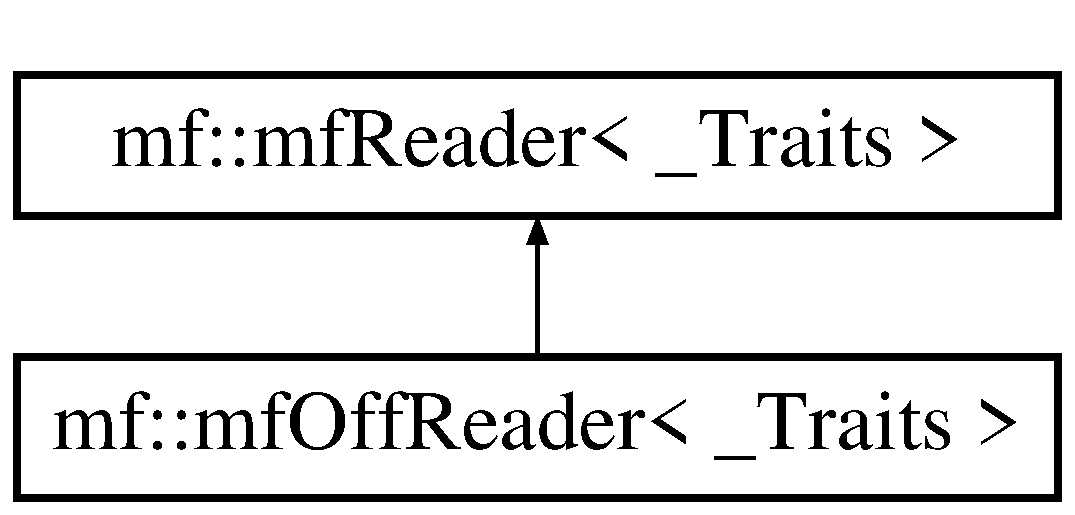
\includegraphics[height=2.000000cm]{classmf_1_1mfOffReader}
\end{center}
\end{figure}
\subsection*{Public Types}
\begin{DoxyCompactItemize}
\item 
typedef \_\-Traits::space \hyperlink{classmf_1_1mfOffReader_ae3a6fa305c9fb47086d819e17a3421d8}{space}
\item 
typedef \_\-Traits::ids \hyperlink{classmf_1_1mfOffReader_abf40a3c998a5b7d45823648315b58d43}{ids}
\item 
typedef \_\-Traits::sVertex \hyperlink{classmf_1_1mfOffReader_a8ecb5f2a5e52408170283b153baff6e1}{sVertex}
\item 
typedef \_\-Traits::sCell \hyperlink{classmf_1_1mfOffReader_acfcb33f834c6ea583daca10ff85c6297}{sCell}
\item 
typedef \_\-Traits::sMesh \hyperlink{classmf_1_1mfOffReader_afd368bca3db54cfe1e60c4a935e6429f}{sMesh}
\end{DoxyCompactItemize}
\subsection*{Public Member Functions}
\begin{DoxyCompactItemize}
\item 
\hyperlink{classmf_1_1mfOffReader_a0df08691ca02b7680795a2c1d188731c}{mfOffReader} ()
\item 
\hyperlink{classmf_1_1mfOffReader_abfef545e8a35d99405608369ba871dfa}{$\sim$mfOffReader} ()
\item 
virtual bool \hyperlink{classmf_1_1mfOffReader_a40cf7f39c327b60827a5858dd3ec8ec9}{read} (\hyperlink{classmf_1_1mfOffReader_afd368bca3db54cfe1e60c4a935e6429f}{sMesh} $\ast$malha, const char $\ast$filename)
\begin{DoxyCompactList}\small\item\em Executa a leitura de um arquivo. \item\end{DoxyCompactList}\end{DoxyCompactItemize}
\subsubsection*{template$<$class \_\-Traits$>$ class mf::mfOffReader$<$ \_\-Traits $>$}



\subsection{Member Typedef Documentation}
\hypertarget{classmf_1_1mfOffReader_abf40a3c998a5b7d45823648315b58d43}{
\index{mf::mfOffReader@{mf::mfOffReader}!ids@{ids}}
\index{ids@{ids}!mf::mfOffReader@{mf::mfOffReader}}
\subsubsection[{ids}]{\setlength{\rightskip}{0pt plus 5cm}template$<$class \_\-Traits $>$ typedef \_\-Traits::ids {\bf mf::mfOffReader}$<$ \_\-Traits $>$::{\bf ids}}}
\label{classmf_1_1mfOffReader_abf40a3c998a5b7d45823648315b58d43}
Id typename definition \hypertarget{classmf_1_1mfOffReader_acfcb33f834c6ea583daca10ff85c6297}{
\index{mf::mfOffReader@{mf::mfOffReader}!sCell@{sCell}}
\index{sCell@{sCell}!mf::mfOffReader@{mf::mfOffReader}}
\subsubsection[{sCell}]{\setlength{\rightskip}{0pt plus 5cm}template$<$class \_\-Traits $>$ typedef \_\-Traits::sCell {\bf mf::mfOffReader}$<$ \_\-Traits $>$::{\bf sCell}}}
\label{classmf_1_1mfOffReader_acfcb33f834c6ea583daca10ff85c6297}
Cell typename definition \hypertarget{classmf_1_1mfOffReader_afd368bca3db54cfe1e60c4a935e6429f}{
\index{mf::mfOffReader@{mf::mfOffReader}!sMesh@{sMesh}}
\index{sMesh@{sMesh}!mf::mfOffReader@{mf::mfOffReader}}
\subsubsection[{sMesh}]{\setlength{\rightskip}{0pt plus 5cm}template$<$class \_\-Traits $>$ typedef \_\-Traits::sMesh {\bf mf::mfOffReader}$<$ \_\-Traits $>$::{\bf sMesh}}}
\label{classmf_1_1mfOffReader_afd368bca3db54cfe1e60c4a935e6429f}
Mesh typename definition 

Reimplemented from \hyperlink{classmf_1_1mfReader}{mf::mfReader$<$ \_\-Traits $>$}.

\hypertarget{classmf_1_1mfOffReader_ae3a6fa305c9fb47086d819e17a3421d8}{
\index{mf::mfOffReader@{mf::mfOffReader}!space@{space}}
\index{space@{space}!mf::mfOffReader@{mf::mfOffReader}}
\subsubsection[{space}]{\setlength{\rightskip}{0pt plus 5cm}template$<$class \_\-Traits $>$ typedef \_\-Traits::space {\bf mf::mfOffReader}$<$ \_\-Traits $>$::{\bf space}}}
\label{classmf_1_1mfOffReader_ae3a6fa305c9fb47086d819e17a3421d8}
Space typename definition \hypertarget{classmf_1_1mfOffReader_a8ecb5f2a5e52408170283b153baff6e1}{
\index{mf::mfOffReader@{mf::mfOffReader}!sVertex@{sVertex}}
\index{sVertex@{sVertex}!mf::mfOffReader@{mf::mfOffReader}}
\subsubsection[{sVertex}]{\setlength{\rightskip}{0pt plus 5cm}template$<$class \_\-Traits $>$ typedef \_\-Traits::sVertex {\bf mf::mfOffReader}$<$ \_\-Traits $>$::{\bf sVertex}}}
\label{classmf_1_1mfOffReader_a8ecb5f2a5e52408170283b153baff6e1}
Vertex typename definition 

\subsection{Constructor \& Destructor Documentation}
\hypertarget{classmf_1_1mfOffReader_a0df08691ca02b7680795a2c1d188731c}{
\index{mf::mfOffReader@{mf::mfOffReader}!mfOffReader@{mfOffReader}}
\index{mfOffReader@{mfOffReader}!mf::mfOffReader@{mf::mfOffReader}}
\subsubsection[{mfOffReader}]{\setlength{\rightskip}{0pt plus 5cm}template$<$class \_\-Traits $>$ {\bf mf::mfOffReader}$<$ \_\-Traits $>$::{\bf mfOffReader} (
\begin{DoxyParamCaption}
{}
\end{DoxyParamCaption}
)}}
\label{classmf_1_1mfOffReader_a0df08691ca02b7680795a2c1d188731c}
Constructor \hypertarget{classmf_1_1mfOffReader_abfef545e8a35d99405608369ba871dfa}{
\index{mf::mfOffReader@{mf::mfOffReader}!$\sim$mfOffReader@{$\sim$mfOffReader}}
\index{$\sim$mfOffReader@{$\sim$mfOffReader}!mf::mfOffReader@{mf::mfOffReader}}
\subsubsection[{$\sim$mfOffReader}]{\setlength{\rightskip}{0pt plus 5cm}template$<$class \_\-Traits $>$ {\bf mf::mfOffReader}$<$ \_\-Traits $>$::$\sim${\bf mfOffReader} (
\begin{DoxyParamCaption}
{}
\end{DoxyParamCaption}
)}}
\label{classmf_1_1mfOffReader_abfef545e8a35d99405608369ba871dfa}
Destructor 

\subsection{Member Function Documentation}
\hypertarget{classmf_1_1mfOffReader_a40cf7f39c327b60827a5858dd3ec8ec9}{
\index{mf::mfOffReader@{mf::mfOffReader}!read@{read}}
\index{read@{read}!mf::mfOffReader@{mf::mfOffReader}}
\subsubsection[{read}]{\setlength{\rightskip}{0pt plus 5cm}template$<$class \_\-Traits $>$ bool {\bf mf::mfOffReader}$<$ \_\-Traits $>$::read (
\begin{DoxyParamCaption}
\item[{{\bf sMesh} $\ast$}]{malha, }
\item[{const char $\ast$}]{filename}
\end{DoxyParamCaption}
)\hspace{0.3cm}{\ttfamily  \mbox{[}virtual\mbox{]}}}}
\label{classmf_1_1mfOffReader_a40cf7f39c327b60827a5858dd3ec8ec9}


Executa a leitura de um arquivo. 

Paraetros de entrada: malha : endereco de memoria de destino da malha a ser carregada. Ja deve estar alocado. filename : nome do arquivo da malha. 

Implements \hyperlink{classmf_1_1mfReader_a0e0c3224a06b06a8fb82be4f0f4a2e00}{mf::mfReader$<$ \_\-Traits $>$}.



The documentation for this class was generated from the following file:\begin{DoxyCompactItemize}
\item 
mfOffReader.h\end{DoxyCompactItemize}

\hypertarget{classmf_1_1mfOffWriter}{
\section{mf::mfOffWriter$<$ \_\-Traits $>$ Class Template Reference}
\label{classmf_1_1mfOffWriter}\index{mf::mfOffWriter@{mf::mfOffWriter}}
}


Salva malhas em arquivo do tipo OFF sem dados.  




{\ttfamily \#include $<$mfOffWriter.h$>$}

Inheritance diagram for mf::mfOffWriter$<$ \_\-Traits $>$:\begin{figure}[H]
\begin{center}
\leavevmode
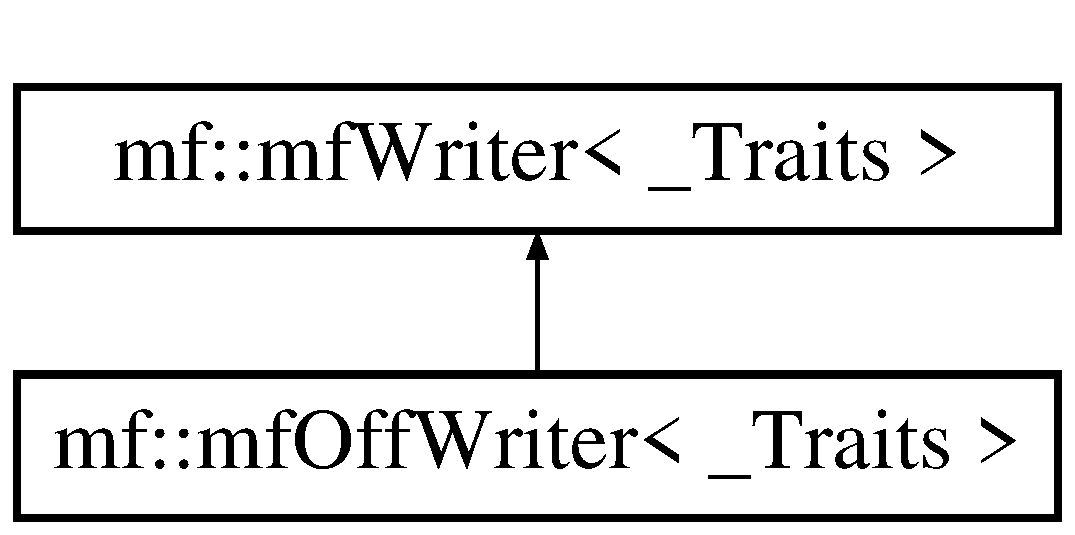
\includegraphics[height=2.000000cm]{classmf_1_1mfOffWriter}
\end{center}
\end{figure}
\subsection*{Public Types}
\begin{DoxyCompactItemize}
\item 
typedef \_\-Traits::space \hyperlink{classmf_1_1mfOffWriter_a4d6664b3f8150c35af57aed9a237c9ab}{space}
\item 
typedef \_\-Traits::ids \hyperlink{classmf_1_1mfOffWriter_ab4a116099ef81a112f35ab9d7d74a998}{ids}
\item 
typedef \_\-Traits::sVertex \hyperlink{classmf_1_1mfOffWriter_a104afc778e21da1edcad11aac363f23e}{sVertex}
\item 
typedef \_\-Traits::sCell \hyperlink{classmf_1_1mfOffWriter_a310a1b7e2284f9d36c931bf47695b980}{sCell}
\item 
typedef \_\-Traits::sMesh \hyperlink{classmf_1_1mfOffWriter_a5dee9306e438bf1819fb9823f6123b5c}{sMesh}
\end{DoxyCompactItemize}
\subsection*{Public Member Functions}
\begin{DoxyCompactItemize}
\item 
\hyperlink{classmf_1_1mfOffWriter_a70b0c81bf8c8a8837d0eb3868381796d}{mfOffWriter} ()
\item 
\hyperlink{classmf_1_1mfOffWriter_a6cd3f70c44f588ef1ba08f8dfaf89a98}{$\sim$mfOffWriter} ()
\item 
virtual bool \hyperlink{classmf_1_1mfOffWriter_ad3fe52bf8870c31c1b9f71431a56af8a}{write} (\hyperlink{classmf_1_1mfOffWriter_a5dee9306e438bf1819fb9823f6123b5c}{sMesh} $\ast$malha, const char $\ast$filename)
\begin{DoxyCompactList}\small\item\em Executa a escrita de um arquivo (salva uma malha) \item\end{DoxyCompactList}\end{DoxyCompactItemize}


\subsection{Detailed Description}
\subsubsection*{template$<$class \_\-Traits$>$ class mf::mfOffWriter$<$ \_\-Traits $>$}

Salva malhas em arquivo do tipo OFF sem dados. 

\subsection{Member Typedef Documentation}
\hypertarget{classmf_1_1mfOffWriter_ab4a116099ef81a112f35ab9d7d74a998}{
\index{mf::mfOffWriter@{mf::mfOffWriter}!ids@{ids}}
\index{ids@{ids}!mf::mfOffWriter@{mf::mfOffWriter}}
\subsubsection[{ids}]{\setlength{\rightskip}{0pt plus 5cm}template$<$class \_\-Traits $>$ typedef \_\-Traits::ids {\bf mf::mfOffWriter}$<$ \_\-Traits $>$::{\bf ids}}}
\label{classmf_1_1mfOffWriter_ab4a116099ef81a112f35ab9d7d74a998}
Id typename definition \hypertarget{classmf_1_1mfOffWriter_a310a1b7e2284f9d36c931bf47695b980}{
\index{mf::mfOffWriter@{mf::mfOffWriter}!sCell@{sCell}}
\index{sCell@{sCell}!mf::mfOffWriter@{mf::mfOffWriter}}
\subsubsection[{sCell}]{\setlength{\rightskip}{0pt plus 5cm}template$<$class \_\-Traits $>$ typedef \_\-Traits::sCell {\bf mf::mfOffWriter}$<$ \_\-Traits $>$::{\bf sCell}}}
\label{classmf_1_1mfOffWriter_a310a1b7e2284f9d36c931bf47695b980}
Cell typename definition \hypertarget{classmf_1_1mfOffWriter_a5dee9306e438bf1819fb9823f6123b5c}{
\index{mf::mfOffWriter@{mf::mfOffWriter}!sMesh@{sMesh}}
\index{sMesh@{sMesh}!mf::mfOffWriter@{mf::mfOffWriter}}
\subsubsection[{sMesh}]{\setlength{\rightskip}{0pt plus 5cm}template$<$class \_\-Traits $>$ typedef \_\-Traits::sMesh {\bf mf::mfOffWriter}$<$ \_\-Traits $>$::{\bf sMesh}}}
\label{classmf_1_1mfOffWriter_a5dee9306e438bf1819fb9823f6123b5c}
Mesh typename definition 

Reimplemented from \hyperlink{classmf_1_1mfWriter}{mf::mfWriter$<$ \_\-Traits $>$}.

\hypertarget{classmf_1_1mfOffWriter_a4d6664b3f8150c35af57aed9a237c9ab}{
\index{mf::mfOffWriter@{mf::mfOffWriter}!space@{space}}
\index{space@{space}!mf::mfOffWriter@{mf::mfOffWriter}}
\subsubsection[{space}]{\setlength{\rightskip}{0pt plus 5cm}template$<$class \_\-Traits $>$ typedef \_\-Traits::space {\bf mf::mfOffWriter}$<$ \_\-Traits $>$::{\bf space}}}
\label{classmf_1_1mfOffWriter_a4d6664b3f8150c35af57aed9a237c9ab}
Space typename definition \hypertarget{classmf_1_1mfOffWriter_a104afc778e21da1edcad11aac363f23e}{
\index{mf::mfOffWriter@{mf::mfOffWriter}!sVertex@{sVertex}}
\index{sVertex@{sVertex}!mf::mfOffWriter@{mf::mfOffWriter}}
\subsubsection[{sVertex}]{\setlength{\rightskip}{0pt plus 5cm}template$<$class \_\-Traits $>$ typedef \_\-Traits::sVertex {\bf mf::mfOffWriter}$<$ \_\-Traits $>$::{\bf sVertex}}}
\label{classmf_1_1mfOffWriter_a104afc778e21da1edcad11aac363f23e}
Vertex typename definition 

\subsection{Constructor \& Destructor Documentation}
\hypertarget{classmf_1_1mfOffWriter_a70b0c81bf8c8a8837d0eb3868381796d}{
\index{mf::mfOffWriter@{mf::mfOffWriter}!mfOffWriter@{mfOffWriter}}
\index{mfOffWriter@{mfOffWriter}!mf::mfOffWriter@{mf::mfOffWriter}}
\subsubsection[{mfOffWriter}]{\setlength{\rightskip}{0pt plus 5cm}template$<$class \_\-Traits $>$ {\bf mf::mfOffWriter}$<$ \_\-Traits $>$::{\bf mfOffWriter} (
\begin{DoxyParamCaption}
{}
\end{DoxyParamCaption}
)}}
\label{classmf_1_1mfOffWriter_a70b0c81bf8c8a8837d0eb3868381796d}
Constructor \hypertarget{classmf_1_1mfOffWriter_a6cd3f70c44f588ef1ba08f8dfaf89a98}{
\index{mf::mfOffWriter@{mf::mfOffWriter}!$\sim$mfOffWriter@{$\sim$mfOffWriter}}
\index{$\sim$mfOffWriter@{$\sim$mfOffWriter}!mf::mfOffWriter@{mf::mfOffWriter}}
\subsubsection[{$\sim$mfOffWriter}]{\setlength{\rightskip}{0pt plus 5cm}template$<$class \_\-Traits $>$ {\bf mf::mfOffWriter}$<$ \_\-Traits $>$::$\sim${\bf mfOffWriter} (
\begin{DoxyParamCaption}
{}
\end{DoxyParamCaption}
)}}
\label{classmf_1_1mfOffWriter_a6cd3f70c44f588ef1ba08f8dfaf89a98}
Destructor 

\subsection{Member Function Documentation}
\hypertarget{classmf_1_1mfOffWriter_ad3fe52bf8870c31c1b9f71431a56af8a}{
\index{mf::mfOffWriter@{mf::mfOffWriter}!write@{write}}
\index{write@{write}!mf::mfOffWriter@{mf::mfOffWriter}}
\subsubsection[{write}]{\setlength{\rightskip}{0pt plus 5cm}template$<$class \_\-Traits $>$ bool {\bf mf::mfOffWriter}$<$ \_\-Traits $>$::write (
\begin{DoxyParamCaption}
\item[{{\bf sMesh} $\ast$}]{malha, }
\item[{const char $\ast$}]{filename}
\end{DoxyParamCaption}
)\hspace{0.3cm}{\ttfamily  \mbox{[}virtual\mbox{]}}}}
\label{classmf_1_1mfOffWriter_ad3fe52bf8870c31c1b9f71431a56af8a}


Executa a escrita de um arquivo (salva uma malha) 

Paraetros de entrada: malha : endereco de memoria da malha a ser salva. filename : nome do arquivo da malha. (destino) 

Implements \hyperlink{classmf_1_1mfWriter_a85d6c59bdb8fec69222e4157c299256c}{mf::mfWriter$<$ \_\-Traits $>$}.



The documentation for this class was generated from the following file:\begin{DoxyCompactItemize}
\item 
mfOffWriter.h\end{DoxyCompactItemize}

\hypertarget{classmf_1_1mfPlyReader}{
\section{mf::mfPlyReader$<$ \_\-Traits $>$ Class Template Reference}
\label{classmf_1_1mfPlyReader}\index{mf::mfPlyReader@{mf::mfPlyReader}}
}
Inheritance diagram for mf::mfPlyReader$<$ \_\-Traits $>$:\begin{figure}[H]
\begin{center}
\leavevmode
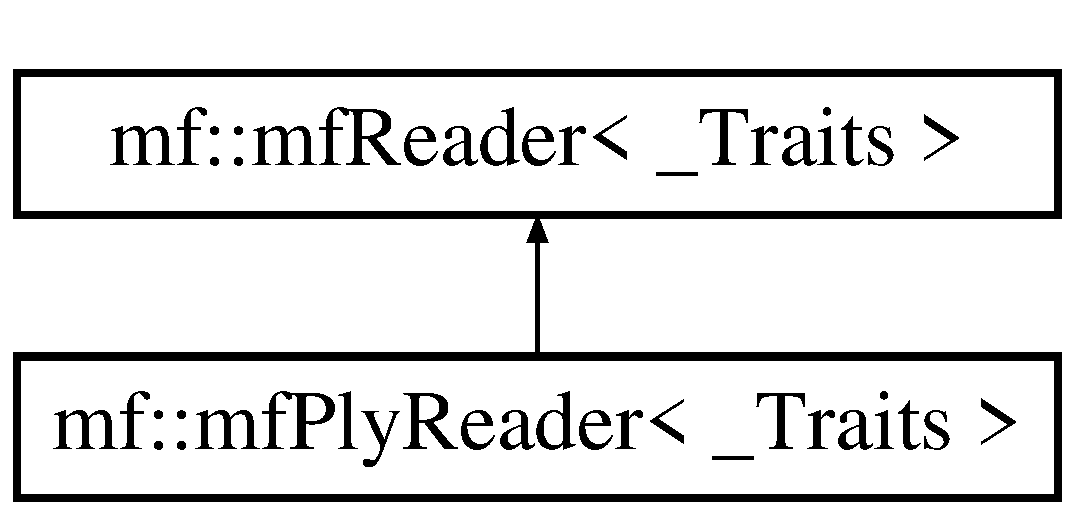
\includegraphics[height=2.000000cm]{classmf_1_1mfPlyReader}
\end{center}
\end{figure}
\subsection*{Public Types}
\begin{DoxyCompactItemize}
\item 
typedef \_\-Traits::space \hyperlink{classmf_1_1mfPlyReader_a148c30ff68212588f695b3391ec7d9f1}{space}
\item 
typedef \_\-Traits::ids \hyperlink{classmf_1_1mfPlyReader_a74dd0c085b152407ff3b92ba7bc672e5}{ids}
\item 
typedef \_\-Traits::sVertex \hyperlink{classmf_1_1mfPlyReader_a4a435b3ad40564d7b5965aad2d0ad292}{sVertex}
\item 
typedef \_\-Traits::sCell \hyperlink{classmf_1_1mfPlyReader_a4ecabd9e906019c1aac0133077fa2409}{sCell}
\item 
typedef \_\-Traits::sMesh \hyperlink{classmf_1_1mfPlyReader_ac1d8f2f32769b5966ac4da1d1c8ee66b}{sMesh}
\end{DoxyCompactItemize}
\subsection*{Public Member Functions}
\begin{DoxyCompactItemize}
\item 
\hyperlink{classmf_1_1mfPlyReader_aae0df7bc479f38fbf9aaa280c73053dc}{mfPlyReader} ()
\item 
\hyperlink{classmf_1_1mfPlyReader_af076b0b7b6ad7868328f9f4482cb666d}{$\sim$mfPlyReader} ()
\item 
virtual bool \hyperlink{classmf_1_1mfPlyReader_ad4aa817979acdfdc6570d2badb288bda}{read} (\hyperlink{classmf_1_1mfPlyReader_ac1d8f2f32769b5966ac4da1d1c8ee66b}{sMesh} $\ast$malha, const char $\ast$filename)
\begin{DoxyCompactList}\small\item\em Executa a leitura de um arquivo. \item\end{DoxyCompactList}\item 
\hypertarget{classmf_1_1mfPlyReader_a924e1c0f8991f301cb54b57aebb2b8c3}{
virtual bool {\bfseries read} (\hyperlink{classmf_1_1mfPlyReader_ac1d8f2f32769b5966ac4da1d1c8ee66b}{sMesh} $\ast$malha, const char $\ast$filename, int cellDimension)}
\label{classmf_1_1mfPlyReader_a924e1c0f8991f301cb54b57aebb2b8c3}

\end{DoxyCompactItemize}
\subsubsection*{template$<$class \_\-Traits$>$ class mf::mfPlyReader$<$ \_\-Traits $>$}



\subsection{Member Typedef Documentation}
\hypertarget{classmf_1_1mfPlyReader_a74dd0c085b152407ff3b92ba7bc672e5}{
\index{mf::mfPlyReader@{mf::mfPlyReader}!ids@{ids}}
\index{ids@{ids}!mf::mfPlyReader@{mf::mfPlyReader}}
\subsubsection[{ids}]{\setlength{\rightskip}{0pt plus 5cm}template$<$class \_\-Traits $>$ typedef \_\-Traits::ids {\bf mf::mfPlyReader}$<$ \_\-Traits $>$::{\bf ids}}}
\label{classmf_1_1mfPlyReader_a74dd0c085b152407ff3b92ba7bc672e5}
Id typename definition \hypertarget{classmf_1_1mfPlyReader_a4ecabd9e906019c1aac0133077fa2409}{
\index{mf::mfPlyReader@{mf::mfPlyReader}!sCell@{sCell}}
\index{sCell@{sCell}!mf::mfPlyReader@{mf::mfPlyReader}}
\subsubsection[{sCell}]{\setlength{\rightskip}{0pt plus 5cm}template$<$class \_\-Traits $>$ typedef \_\-Traits::sCell {\bf mf::mfPlyReader}$<$ \_\-Traits $>$::{\bf sCell}}}
\label{classmf_1_1mfPlyReader_a4ecabd9e906019c1aac0133077fa2409}
Cell typename definition \hypertarget{classmf_1_1mfPlyReader_ac1d8f2f32769b5966ac4da1d1c8ee66b}{
\index{mf::mfPlyReader@{mf::mfPlyReader}!sMesh@{sMesh}}
\index{sMesh@{sMesh}!mf::mfPlyReader@{mf::mfPlyReader}}
\subsubsection[{sMesh}]{\setlength{\rightskip}{0pt plus 5cm}template$<$class \_\-Traits $>$ typedef \_\-Traits::sMesh {\bf mf::mfPlyReader}$<$ \_\-Traits $>$::{\bf sMesh}}}
\label{classmf_1_1mfPlyReader_ac1d8f2f32769b5966ac4da1d1c8ee66b}
Mesh typename definition 

Reimplemented from \hyperlink{classmf_1_1mfReader}{mf::mfReader$<$ \_\-Traits $>$}.

\hypertarget{classmf_1_1mfPlyReader_a148c30ff68212588f695b3391ec7d9f1}{
\index{mf::mfPlyReader@{mf::mfPlyReader}!space@{space}}
\index{space@{space}!mf::mfPlyReader@{mf::mfPlyReader}}
\subsubsection[{space}]{\setlength{\rightskip}{0pt plus 5cm}template$<$class \_\-Traits $>$ typedef \_\-Traits::space {\bf mf::mfPlyReader}$<$ \_\-Traits $>$::{\bf space}}}
\label{classmf_1_1mfPlyReader_a148c30ff68212588f695b3391ec7d9f1}
Space typename definition \hypertarget{classmf_1_1mfPlyReader_a4a435b3ad40564d7b5965aad2d0ad292}{
\index{mf::mfPlyReader@{mf::mfPlyReader}!sVertex@{sVertex}}
\index{sVertex@{sVertex}!mf::mfPlyReader@{mf::mfPlyReader}}
\subsubsection[{sVertex}]{\setlength{\rightskip}{0pt plus 5cm}template$<$class \_\-Traits $>$ typedef \_\-Traits::sVertex {\bf mf::mfPlyReader}$<$ \_\-Traits $>$::{\bf sVertex}}}
\label{classmf_1_1mfPlyReader_a4a435b3ad40564d7b5965aad2d0ad292}
Vertex typename definition 

\subsection{Constructor \& Destructor Documentation}
\hypertarget{classmf_1_1mfPlyReader_aae0df7bc479f38fbf9aaa280c73053dc}{
\index{mf::mfPlyReader@{mf::mfPlyReader}!mfPlyReader@{mfPlyReader}}
\index{mfPlyReader@{mfPlyReader}!mf::mfPlyReader@{mf::mfPlyReader}}
\subsubsection[{mfPlyReader}]{\setlength{\rightskip}{0pt plus 5cm}template$<$class \_\-Traits $>$ {\bf mf::mfPlyReader}$<$ \_\-Traits $>$::{\bf mfPlyReader} (
\begin{DoxyParamCaption}
{}
\end{DoxyParamCaption}
)}}
\label{classmf_1_1mfPlyReader_aae0df7bc479f38fbf9aaa280c73053dc}
Constructor \hypertarget{classmf_1_1mfPlyReader_af076b0b7b6ad7868328f9f4482cb666d}{
\index{mf::mfPlyReader@{mf::mfPlyReader}!$\sim$mfPlyReader@{$\sim$mfPlyReader}}
\index{$\sim$mfPlyReader@{$\sim$mfPlyReader}!mf::mfPlyReader@{mf::mfPlyReader}}
\subsubsection[{$\sim$mfPlyReader}]{\setlength{\rightskip}{0pt plus 5cm}template$<$class \_\-Traits $>$ {\bf mf::mfPlyReader}$<$ \_\-Traits $>$::$\sim${\bf mfPlyReader} (
\begin{DoxyParamCaption}
{}
\end{DoxyParamCaption}
)}}
\label{classmf_1_1mfPlyReader_af076b0b7b6ad7868328f9f4482cb666d}
Destructor 

\subsection{Member Function Documentation}
\hypertarget{classmf_1_1mfPlyReader_ad4aa817979acdfdc6570d2badb288bda}{
\index{mf::mfPlyReader@{mf::mfPlyReader}!read@{read}}
\index{read@{read}!mf::mfPlyReader@{mf::mfPlyReader}}
\subsubsection[{read}]{\setlength{\rightskip}{0pt plus 5cm}template$<$class \_\-Traits $>$ bool {\bf mf::mfPlyReader}$<$ \_\-Traits $>$::read (
\begin{DoxyParamCaption}
\item[{{\bf sMesh} $\ast$}]{malha, }
\item[{const char $\ast$}]{filename}
\end{DoxyParamCaption}
)\hspace{0.3cm}{\ttfamily  \mbox{[}virtual\mbox{]}}}}
\label{classmf_1_1mfPlyReader_ad4aa817979acdfdc6570d2badb288bda}


Executa a leitura de um arquivo. 

Paraetros de entrada: malha : endereco de memoria de destino da malha a ser carregada. Ja deve estar alocado. filename : nome do arquivo da malha. 

Implements \hyperlink{classmf_1_1mfReader_a0e0c3224a06b06a8fb82be4f0f4a2e00}{mf::mfReader$<$ \_\-Traits $>$}.



The documentation for this class was generated from the following file:\begin{DoxyCompactItemize}
\item 
mfPlyReader.h\end{DoxyCompactItemize}

\hypertarget{classmf_1_1mfPolyDataReader}{
\section{mf::mfPolyDataReader$<$ \_\-Traits $>$ Class Template Reference}
\label{classmf_1_1mfPolyDataReader}\index{mf::mfPolyDataReader@{mf::mfPolyDataReader}}
}
Inheritance diagram for mf::mfPolyDataReader$<$ \_\-Traits $>$:\begin{figure}[H]
\begin{center}
\leavevmode
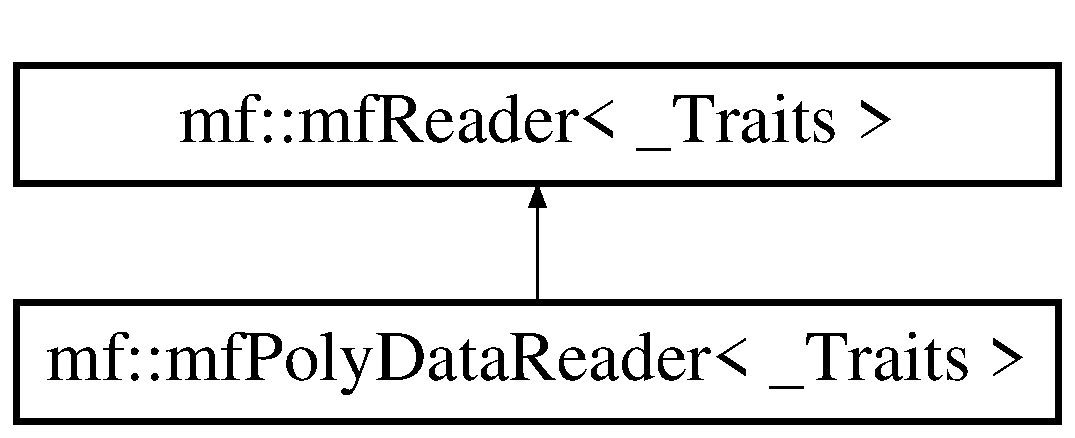
\includegraphics[height=2.000000cm]{classmf_1_1mfPolyDataReader}
\end{center}
\end{figure}
\subsection*{Classes}
\begin{DoxyCompactItemize}
\item 
class {\bfseries sObject}
\item 
class {\bfseries sObjectCompare}
\end{DoxyCompactItemize}
\subsection*{Public Types}
\begin{DoxyCompactItemize}
\item 
typedef \_\-Traits::space \hyperlink{classmf_1_1mfPolyDataReader_ab5c4255c5e508f817feaacc8aafd8bb9}{space}
\item 
typedef \_\-Traits::ids \hyperlink{classmf_1_1mfPolyDataReader_a1d1a716d5dd72816147f86518dcd20a0}{ids}
\item 
typedef \_\-Traits::sVertex \hyperlink{classmf_1_1mfPolyDataReader_a51d78f02cab20097f62a78134bf7d0f3}{sVertex}
\item 
typedef \_\-Traits::sCell \hyperlink{classmf_1_1mfPolyDataReader_a712889726fe13348e13c23990d0d412b}{sCell}
\item 
typedef \_\-Traits::sMesh \hyperlink{classmf_1_1mfPolyDataReader_a5343a659b464b89fc0c8b58ee56ed568}{sMesh}
\item 
typedef \_\-Traits::sGeometric \hyperlink{classmf_1_1mfPolyDataReader_af064c717a7483939d46991da73d4304d}{sGeometric}
\end{DoxyCompactItemize}
\subsection*{Public Member Functions}
\begin{DoxyCompactItemize}
\item 
\hyperlink{classmf_1_1mfPolyDataReader_a5179b5d325985e2ee3d51c05e1434e67}{mfPolyDataReader} ()
\item 
\hyperlink{classmf_1_1mfPolyDataReader_a6c7cb050280ccbf0700e40a1a4d54b84}{$\sim$mfPolyDataReader} ()
\item 
\hypertarget{classmf_1_1mfPolyDataReader_ab2857fae25ff16cfe8b621e6d89395b6}{
void {\bfseries checkPoints} (bool value)}
\label{classmf_1_1mfPolyDataReader_ab2857fae25ff16cfe8b621e6d89395b6}

\item 
virtual bool \hyperlink{classmf_1_1mfPolyDataReader_a2c013ff82158ddc91ab451257a3051d0}{read} (\hyperlink{classmf_1_1mfPolyDataReader_a5343a659b464b89fc0c8b58ee56ed568}{sMesh} $\ast$malha, const char $\ast$filename)
\begin{DoxyCompactList}\small\item\em Executa a leitura de um arquivo. \item\end{DoxyCompactList}\end{DoxyCompactItemize}
\subsubsection*{template$<$class \_\-Traits$>$ class mf::mfPolyDataReader$<$ \_\-Traits $>$}



\subsection{Member Typedef Documentation}
\hypertarget{classmf_1_1mfPolyDataReader_a1d1a716d5dd72816147f86518dcd20a0}{
\index{mf::mfPolyDataReader@{mf::mfPolyDataReader}!ids@{ids}}
\index{ids@{ids}!mf::mfPolyDataReader@{mf::mfPolyDataReader}}
\subsubsection[{ids}]{\setlength{\rightskip}{0pt plus 5cm}template$<$class \_\-Traits $>$ typedef \_\-Traits::ids {\bf mf::mfPolyDataReader}$<$ \_\-Traits $>$::{\bf ids}}}
\label{classmf_1_1mfPolyDataReader_a1d1a716d5dd72816147f86518dcd20a0}
Id typename definition \hypertarget{classmf_1_1mfPolyDataReader_a712889726fe13348e13c23990d0d412b}{
\index{mf::mfPolyDataReader@{mf::mfPolyDataReader}!sCell@{sCell}}
\index{sCell@{sCell}!mf::mfPolyDataReader@{mf::mfPolyDataReader}}
\subsubsection[{sCell}]{\setlength{\rightskip}{0pt plus 5cm}template$<$class \_\-Traits $>$ typedef \_\-Traits::sCell {\bf mf::mfPolyDataReader}$<$ \_\-Traits $>$::{\bf sCell}}}
\label{classmf_1_1mfPolyDataReader_a712889726fe13348e13c23990d0d412b}
Cell typename definition \hypertarget{classmf_1_1mfPolyDataReader_af064c717a7483939d46991da73d4304d}{
\index{mf::mfPolyDataReader@{mf::mfPolyDataReader}!sGeometric@{sGeometric}}
\index{sGeometric@{sGeometric}!mf::mfPolyDataReader@{mf::mfPolyDataReader}}
\subsubsection[{sGeometric}]{\setlength{\rightskip}{0pt plus 5cm}template$<$class \_\-Traits $>$ typedef \_\-Traits::sGeometric {\bf mf::mfPolyDataReader}$<$ \_\-Traits $>$::{\bf sGeometric}}}
\label{classmf_1_1mfPolyDataReader_af064c717a7483939d46991da73d4304d}
Geometric typename definition \hypertarget{classmf_1_1mfPolyDataReader_a5343a659b464b89fc0c8b58ee56ed568}{
\index{mf::mfPolyDataReader@{mf::mfPolyDataReader}!sMesh@{sMesh}}
\index{sMesh@{sMesh}!mf::mfPolyDataReader@{mf::mfPolyDataReader}}
\subsubsection[{sMesh}]{\setlength{\rightskip}{0pt plus 5cm}template$<$class \_\-Traits $>$ typedef \_\-Traits::sMesh {\bf mf::mfPolyDataReader}$<$ \_\-Traits $>$::{\bf sMesh}}}
\label{classmf_1_1mfPolyDataReader_a5343a659b464b89fc0c8b58ee56ed568}
Mesh typename definition 

Reimplemented from \hyperlink{classmf_1_1mfReader}{mf::mfReader$<$ \_\-Traits $>$}.

\hypertarget{classmf_1_1mfPolyDataReader_ab5c4255c5e508f817feaacc8aafd8bb9}{
\index{mf::mfPolyDataReader@{mf::mfPolyDataReader}!space@{space}}
\index{space@{space}!mf::mfPolyDataReader@{mf::mfPolyDataReader}}
\subsubsection[{space}]{\setlength{\rightskip}{0pt plus 5cm}template$<$class \_\-Traits $>$ typedef \_\-Traits::space {\bf mf::mfPolyDataReader}$<$ \_\-Traits $>$::{\bf space}}}
\label{classmf_1_1mfPolyDataReader_ab5c4255c5e508f817feaacc8aafd8bb9}
Space typename definition \hypertarget{classmf_1_1mfPolyDataReader_a51d78f02cab20097f62a78134bf7d0f3}{
\index{mf::mfPolyDataReader@{mf::mfPolyDataReader}!sVertex@{sVertex}}
\index{sVertex@{sVertex}!mf::mfPolyDataReader@{mf::mfPolyDataReader}}
\subsubsection[{sVertex}]{\setlength{\rightskip}{0pt plus 5cm}template$<$class \_\-Traits $>$ typedef \_\-Traits::sVertex {\bf mf::mfPolyDataReader}$<$ \_\-Traits $>$::{\bf sVertex}}}
\label{classmf_1_1mfPolyDataReader_a51d78f02cab20097f62a78134bf7d0f3}
Vertex typename definition 

\subsection{Constructor \& Destructor Documentation}
\hypertarget{classmf_1_1mfPolyDataReader_a5179b5d325985e2ee3d51c05e1434e67}{
\index{mf::mfPolyDataReader@{mf::mfPolyDataReader}!mfPolyDataReader@{mfPolyDataReader}}
\index{mfPolyDataReader@{mfPolyDataReader}!mf::mfPolyDataReader@{mf::mfPolyDataReader}}
\subsubsection[{mfPolyDataReader}]{\setlength{\rightskip}{0pt plus 5cm}template$<$class \_\-Traits $>$ {\bf mf::mfPolyDataReader}$<$ \_\-Traits $>$::{\bf mfPolyDataReader} (
\begin{DoxyParamCaption}
{}
\end{DoxyParamCaption}
)}}
\label{classmf_1_1mfPolyDataReader_a5179b5d325985e2ee3d51c05e1434e67}
Constructor \hypertarget{classmf_1_1mfPolyDataReader_a6c7cb050280ccbf0700e40a1a4d54b84}{
\index{mf::mfPolyDataReader@{mf::mfPolyDataReader}!$\sim$mfPolyDataReader@{$\sim$mfPolyDataReader}}
\index{$\sim$mfPolyDataReader@{$\sim$mfPolyDataReader}!mf::mfPolyDataReader@{mf::mfPolyDataReader}}
\subsubsection[{$\sim$mfPolyDataReader}]{\setlength{\rightskip}{0pt plus 5cm}template$<$class \_\-Traits $>$ {\bf mf::mfPolyDataReader}$<$ \_\-Traits $>$::$\sim${\bf mfPolyDataReader} (
\begin{DoxyParamCaption}
{}
\end{DoxyParamCaption}
)}}
\label{classmf_1_1mfPolyDataReader_a6c7cb050280ccbf0700e40a1a4d54b84}
Destructor 

\subsection{Member Function Documentation}
\hypertarget{classmf_1_1mfPolyDataReader_a2c013ff82158ddc91ab451257a3051d0}{
\index{mf::mfPolyDataReader@{mf::mfPolyDataReader}!read@{read}}
\index{read@{read}!mf::mfPolyDataReader@{mf::mfPolyDataReader}}
\subsubsection[{read}]{\setlength{\rightskip}{0pt plus 5cm}template$<$class \_\-Traits $>$ bool {\bf mf::mfPolyDataReader}$<$ \_\-Traits $>$::read (
\begin{DoxyParamCaption}
\item[{{\bf sMesh} $\ast$}]{malha, }
\item[{const char $\ast$}]{filename}
\end{DoxyParamCaption}
)\hspace{0.3cm}{\ttfamily  \mbox{[}virtual\mbox{]}}}}
\label{classmf_1_1mfPolyDataReader_a2c013ff82158ddc91ab451257a3051d0}


Executa a leitura de um arquivo. 

Paraetros de entrada: malha : endereco de memoria de destino da malha a ser carregada. Ja deve estar alocado. filename : nome do arquivo da malha. 

Implements \hyperlink{classmf_1_1mfReader_a0e0c3224a06b06a8fb82be4f0f4a2e00}{mf::mfReader$<$ \_\-Traits $>$}.



The documentation for this class was generated from the following file:\begin{DoxyCompactItemize}
\item 
mfPolyDataReader.h\end{DoxyCompactItemize}

\hypertarget{classmf_1_1mfPolyDataWriter}{
\section{mf::mfPolyDataWriter$<$ \_\-Traits $>$ Class Template Reference}
\label{classmf_1_1mfPolyDataWriter}\index{mf::mfPolyDataWriter@{mf::mfPolyDataWriter}}
}


Salva malhas em arquivo do tipo VTK sem dados.  




{\ttfamily \#include $<$mfPolyDataWriter.h$>$}

Inheritance diagram for mf::mfPolyDataWriter$<$ \_\-Traits $>$:\begin{figure}[H]
\begin{center}
\leavevmode
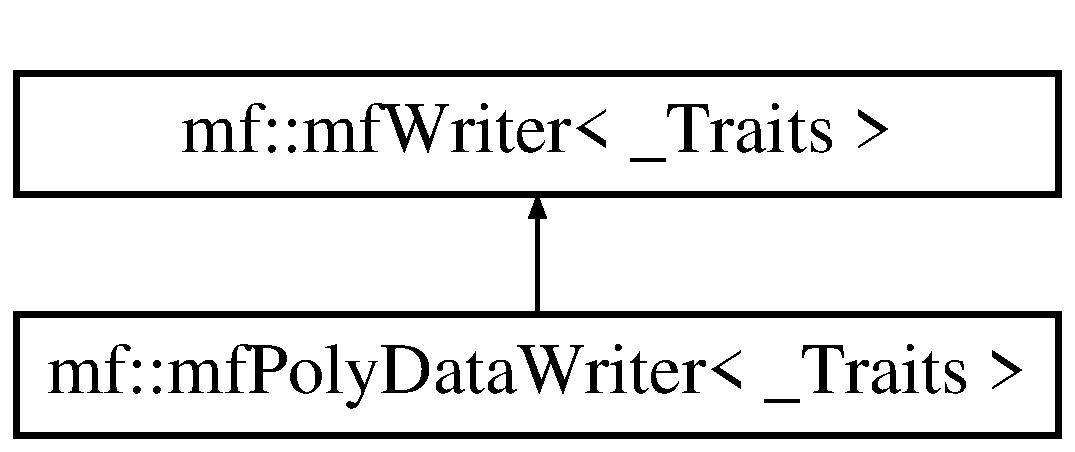
\includegraphics[height=2.000000cm]{classmf_1_1mfPolyDataWriter}
\end{center}
\end{figure}
\subsection*{Public Types}
\begin{DoxyCompactItemize}
\item 
typedef \_\-Traits::space \hyperlink{classmf_1_1mfPolyDataWriter_a386a48d93bcf6f9febdb9730fc67443b}{space}
\item 
typedef \_\-Traits::ids \hyperlink{classmf_1_1mfPolyDataWriter_ae7e024a913c218669ede149f7771f85e}{ids}
\item 
typedef \_\-Traits::sVertex \hyperlink{classmf_1_1mfPolyDataWriter_ad9ede939e471c1075cfed0007cbe027c}{sVertex}
\item 
typedef \_\-Traits::sCell \hyperlink{classmf_1_1mfPolyDataWriter_a271a825b5446e6c388a238e577840920}{sCell}
\item 
typedef \_\-Traits::sMesh \hyperlink{classmf_1_1mfPolyDataWriter_a4ce58a6aa7139b3d903cc453c4585e6f}{sMesh}
\end{DoxyCompactItemize}
\subsection*{Public Member Functions}
\begin{DoxyCompactItemize}
\item 
\hyperlink{classmf_1_1mfPolyDataWriter_a6f343089c2533ecc900d613e6ceedbff}{mfPolyDataWriter} ()
\item 
\hyperlink{classmf_1_1mfPolyDataWriter_af0b6e3370b0f9bfdc8c2c44814538742}{$\sim$mfPolyDataWriter} ()
\item 
virtual bool \hyperlink{classmf_1_1mfPolyDataWriter_a5621f62f1a2811fa1b24da447cf3c5ea}{write} (\hyperlink{classmf_1_1mfPolyDataWriter_a4ce58a6aa7139b3d903cc453c4585e6f}{sMesh} $\ast$malha, const char $\ast$filename)
\begin{DoxyCompactList}\small\item\em Executa a escrita de um arquivo (salva uma malha) \item\end{DoxyCompactList}\end{DoxyCompactItemize}


\subsection{Detailed Description}
\subsubsection*{template$<$class \_\-Traits$>$ class mf::mfPolyDataWriter$<$ \_\-Traits $>$}

Salva malhas em arquivo do tipo VTK sem dados. 

\subsection{Member Typedef Documentation}
\hypertarget{classmf_1_1mfPolyDataWriter_ae7e024a913c218669ede149f7771f85e}{
\index{mf::mfPolyDataWriter@{mf::mfPolyDataWriter}!ids@{ids}}
\index{ids@{ids}!mf::mfPolyDataWriter@{mf::mfPolyDataWriter}}
\subsubsection[{ids}]{\setlength{\rightskip}{0pt plus 5cm}template$<$class \_\-Traits $>$ typedef \_\-Traits::ids {\bf mf::mfPolyDataWriter}$<$ \_\-Traits $>$::{\bf ids}}}
\label{classmf_1_1mfPolyDataWriter_ae7e024a913c218669ede149f7771f85e}
Id typename definition \hypertarget{classmf_1_1mfPolyDataWriter_a271a825b5446e6c388a238e577840920}{
\index{mf::mfPolyDataWriter@{mf::mfPolyDataWriter}!sCell@{sCell}}
\index{sCell@{sCell}!mf::mfPolyDataWriter@{mf::mfPolyDataWriter}}
\subsubsection[{sCell}]{\setlength{\rightskip}{0pt plus 5cm}template$<$class \_\-Traits $>$ typedef \_\-Traits::sCell {\bf mf::mfPolyDataWriter}$<$ \_\-Traits $>$::{\bf sCell}}}
\label{classmf_1_1mfPolyDataWriter_a271a825b5446e6c388a238e577840920}
Cell typename definition \hypertarget{classmf_1_1mfPolyDataWriter_a4ce58a6aa7139b3d903cc453c4585e6f}{
\index{mf::mfPolyDataWriter@{mf::mfPolyDataWriter}!sMesh@{sMesh}}
\index{sMesh@{sMesh}!mf::mfPolyDataWriter@{mf::mfPolyDataWriter}}
\subsubsection[{sMesh}]{\setlength{\rightskip}{0pt plus 5cm}template$<$class \_\-Traits $>$ typedef \_\-Traits::sMesh {\bf mf::mfPolyDataWriter}$<$ \_\-Traits $>$::{\bf sMesh}}}
\label{classmf_1_1mfPolyDataWriter_a4ce58a6aa7139b3d903cc453c4585e6f}
Mesh typename definition 

Reimplemented from \hyperlink{classmf_1_1mfWriter}{mf::mfWriter$<$ \_\-Traits $>$}.

\hypertarget{classmf_1_1mfPolyDataWriter_a386a48d93bcf6f9febdb9730fc67443b}{
\index{mf::mfPolyDataWriter@{mf::mfPolyDataWriter}!space@{space}}
\index{space@{space}!mf::mfPolyDataWriter@{mf::mfPolyDataWriter}}
\subsubsection[{space}]{\setlength{\rightskip}{0pt plus 5cm}template$<$class \_\-Traits $>$ typedef \_\-Traits::space {\bf mf::mfPolyDataWriter}$<$ \_\-Traits $>$::{\bf space}}}
\label{classmf_1_1mfPolyDataWriter_a386a48d93bcf6f9febdb9730fc67443b}
Space typename definition \hypertarget{classmf_1_1mfPolyDataWriter_ad9ede939e471c1075cfed0007cbe027c}{
\index{mf::mfPolyDataWriter@{mf::mfPolyDataWriter}!sVertex@{sVertex}}
\index{sVertex@{sVertex}!mf::mfPolyDataWriter@{mf::mfPolyDataWriter}}
\subsubsection[{sVertex}]{\setlength{\rightskip}{0pt plus 5cm}template$<$class \_\-Traits $>$ typedef \_\-Traits::sVertex {\bf mf::mfPolyDataWriter}$<$ \_\-Traits $>$::{\bf sVertex}}}
\label{classmf_1_1mfPolyDataWriter_ad9ede939e471c1075cfed0007cbe027c}
Vertex typename definition 

\subsection{Constructor \& Destructor Documentation}
\hypertarget{classmf_1_1mfPolyDataWriter_a6f343089c2533ecc900d613e6ceedbff}{
\index{mf::mfPolyDataWriter@{mf::mfPolyDataWriter}!mfPolyDataWriter@{mfPolyDataWriter}}
\index{mfPolyDataWriter@{mfPolyDataWriter}!mf::mfPolyDataWriter@{mf::mfPolyDataWriter}}
\subsubsection[{mfPolyDataWriter}]{\setlength{\rightskip}{0pt plus 5cm}template$<$class \_\-Traits $>$ {\bf mf::mfPolyDataWriter}$<$ \_\-Traits $>$::{\bf mfPolyDataWriter} (
\begin{DoxyParamCaption}
{}
\end{DoxyParamCaption}
)}}
\label{classmf_1_1mfPolyDataWriter_a6f343089c2533ecc900d613e6ceedbff}
Constructor \hypertarget{classmf_1_1mfPolyDataWriter_af0b6e3370b0f9bfdc8c2c44814538742}{
\index{mf::mfPolyDataWriter@{mf::mfPolyDataWriter}!$\sim$mfPolyDataWriter@{$\sim$mfPolyDataWriter}}
\index{$\sim$mfPolyDataWriter@{$\sim$mfPolyDataWriter}!mf::mfPolyDataWriter@{mf::mfPolyDataWriter}}
\subsubsection[{$\sim$mfPolyDataWriter}]{\setlength{\rightskip}{0pt plus 5cm}template$<$class \_\-Traits $>$ {\bf mf::mfPolyDataWriter}$<$ \_\-Traits $>$::$\sim${\bf mfPolyDataWriter} (
\begin{DoxyParamCaption}
{}
\end{DoxyParamCaption}
)}}
\label{classmf_1_1mfPolyDataWriter_af0b6e3370b0f9bfdc8c2c44814538742}
Destructor 

\subsection{Member Function Documentation}
\hypertarget{classmf_1_1mfPolyDataWriter_a5621f62f1a2811fa1b24da447cf3c5ea}{
\index{mf::mfPolyDataWriter@{mf::mfPolyDataWriter}!write@{write}}
\index{write@{write}!mf::mfPolyDataWriter@{mf::mfPolyDataWriter}}
\subsubsection[{write}]{\setlength{\rightskip}{0pt plus 5cm}template$<$class \_\-Traits $>$ bool {\bf mf::mfPolyDataWriter}$<$ \_\-Traits $>$::write (
\begin{DoxyParamCaption}
\item[{{\bf sMesh} $\ast$}]{malha, }
\item[{const char $\ast$}]{filename}
\end{DoxyParamCaption}
)\hspace{0.3cm}{\ttfamily  \mbox{[}virtual\mbox{]}}}}
\label{classmf_1_1mfPolyDataWriter_a5621f62f1a2811fa1b24da447cf3c5ea}


Executa a escrita de um arquivo (salva uma malha) 

Paraetros de entrada: malha : endereco de memoria da malha a ser salva. filename : nome do arquivo da malha. (destino) 

Implements \hyperlink{classmf_1_1mfWriter_a85d6c59bdb8fec69222e4157c299256c}{mf::mfWriter$<$ \_\-Traits $>$}.



The documentation for this class was generated from the following file:\begin{DoxyCompactItemize}
\item 
mfPolyDataWriter.h\end{DoxyCompactItemize}

\hypertarget{classmf_1_1mfQuadCell}{
\section{mf::mfQuadCell$<$ \_\-Traits $>$ Class Template Reference}
\label{classmf_1_1mfQuadCell}\index{mf::mfQuadCell@{mf::mfQuadCell}}
}
Inheritance diagram for mf::mfQuadCell$<$ \_\-Traits $>$:\begin{figure}[H]
\begin{center}
\leavevmode
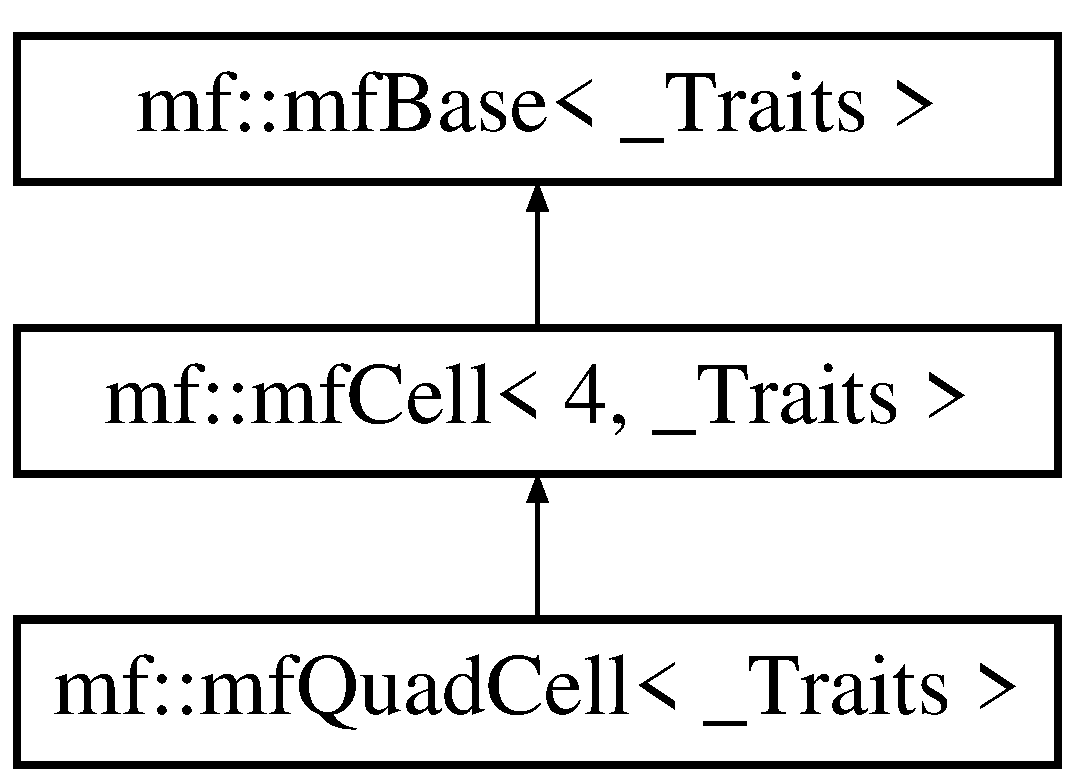
\includegraphics[height=3.000000cm]{classmf_1_1mfQuadCell}
\end{center}
\end{figure}
\subsection*{Public Types}
\begin{DoxyCompactItemize}
\item 
typedef \_\-Traits::ids \hyperlink{classmf_1_1mfQuadCell_a443cbcdcefb50bddded8078d38869040}{ids}
\end{DoxyCompactItemize}
\subsection*{Public Member Functions}
\begin{DoxyCompactItemize}
\item 
\hyperlink{classmf_1_1mfQuadCell_a9b368af5dac34f90ec4bb803624abb08}{mfQuadCell} ()
\item 
virtual \hyperlink{classmf_1_1mfQuadCell_af8546dd501a6b21051b0924667135ed7}{$\sim$mfQuadCell} ()
\item 
\hyperlink{classmf_1_1mfBase_a3b23f16ddf59da0a91ab12cf57c1f111}{ids} \hyperlink{classmf_1_1mfQuadCell_aad6ab1fce113adefd8531daaf5141cae}{getEdgeId} (int index MF\_\-DMUTEXVD)
\item 
void \hyperlink{classmf_1_1mfQuadCell_acdbd1895f8ee380416c289d26a24f6db}{setEdgeId} (int index, \hyperlink{classmf_1_1mfBase_a3b23f16ddf59da0a91ab12cf57c1f111}{ids} edge MF\_\-DMUTEXVD)
\end{DoxyCompactItemize}
\subsection*{Static Public Member Functions}
\begin{DoxyCompactItemize}
\item 
static int \hyperlink{classmf_1_1mfQuadCell_a797da8c9839219488be115b41d9ebe6b}{getDimension} ()
\end{DoxyCompactItemize}
\subsubsection*{template$<$class \_\-Traits$>$ class mf::mfQuadCell$<$ \_\-Traits $>$}



\subsection{Member Typedef Documentation}
\hypertarget{classmf_1_1mfQuadCell_a443cbcdcefb50bddded8078d38869040}{
\index{mf::mfQuadCell@{mf::mfQuadCell}!ids@{ids}}
\index{ids@{ids}!mf::mfQuadCell@{mf::mfQuadCell}}
\subsubsection[{ids}]{\setlength{\rightskip}{0pt plus 5cm}template$<$class \_\-Traits $>$ typedef \_\-Traits ::{\bf ids} {\bf mf::mfQuadCell}$<$ \_\-Traits $>$::{\bf ids}}}
\label{classmf_1_1mfQuadCell_a443cbcdcefb50bddded8078d38869040}
Id typename definition 

Reimplemented from \hyperlink{classmf_1_1mfCell_a9e32102899fb1e6b5e95b08a6c71063f}{mf::mfCell$<$ 4, \_\-Traits $>$}.



\subsection{Constructor \& Destructor Documentation}
\hypertarget{classmf_1_1mfQuadCell_a9b368af5dac34f90ec4bb803624abb08}{
\index{mf::mfQuadCell@{mf::mfQuadCell}!mfQuadCell@{mfQuadCell}}
\index{mfQuadCell@{mfQuadCell}!mf::mfQuadCell@{mf::mfQuadCell}}
\subsubsection[{mfQuadCell}]{\setlength{\rightskip}{0pt plus 5cm}template$<$class \_\-Traits $>$ {\bf mf::mfQuadCell}$<$ \_\-Traits $>$::{\bf mfQuadCell} (
\begin{DoxyParamCaption}
{}
\end{DoxyParamCaption}
)}}
\label{classmf_1_1mfQuadCell_a9b368af5dac34f90ec4bb803624abb08}
Constructor \hypertarget{classmf_1_1mfQuadCell_af8546dd501a6b21051b0924667135ed7}{
\index{mf::mfQuadCell@{mf::mfQuadCell}!$\sim$mfQuadCell@{$\sim$mfQuadCell}}
\index{$\sim$mfQuadCell@{$\sim$mfQuadCell}!mf::mfQuadCell@{mf::mfQuadCell}}
\subsubsection[{$\sim$mfQuadCell}]{\setlength{\rightskip}{0pt plus 5cm}template$<$class \_\-Traits $>$ {\bf mf::mfQuadCell}$<$ \_\-Traits $>$::$\sim${\bf mfQuadCell} (
\begin{DoxyParamCaption}
{}
\end{DoxyParamCaption}
)\hspace{0.3cm}{\ttfamily  \mbox{[}virtual\mbox{]}}}}
\label{classmf_1_1mfQuadCell_af8546dd501a6b21051b0924667135ed7}
Destructor 

\subsection{Member Function Documentation}
\hypertarget{classmf_1_1mfQuadCell_a797da8c9839219488be115b41d9ebe6b}{
\index{mf::mfQuadCell@{mf::mfQuadCell}!getDimension@{getDimension}}
\index{getDimension@{getDimension}!mf::mfQuadCell@{mf::mfQuadCell}}
\subsubsection[{getDimension}]{\setlength{\rightskip}{0pt plus 5cm}template$<$class \_\-Traits $>$ static int {\bf mf::mfQuadCell}$<$ \_\-Traits $>$::getDimension (
\begin{DoxyParamCaption}
{}
\end{DoxyParamCaption}
)\hspace{0.3cm}{\ttfamily  \mbox{[}inline, static\mbox{]}}}}
\label{classmf_1_1mfQuadCell_a797da8c9839219488be115b41d9ebe6b}
Return the dimension of this cell 

Reimplemented from \hyperlink{classmf_1_1mfCell_adca6e1707e9d8487c22b3cd0117791a0}{mf::mfCell$<$ 4, \_\-Traits $>$}.

\hypertarget{classmf_1_1mfQuadCell_aad6ab1fce113adefd8531daaf5141cae}{
\index{mf::mfQuadCell@{mf::mfQuadCell}!getEdgeId@{getEdgeId}}
\index{getEdgeId@{getEdgeId}!mf::mfQuadCell@{mf::mfQuadCell}}
\subsubsection[{getEdgeId}]{\setlength{\rightskip}{0pt plus 5cm}template$<$class \_\-Traits $>$ IDS {\bf mf::mfQuadCell}$<$ \_\-Traits $>$::getEdgeId (
\begin{DoxyParamCaption}
\item[{int index}]{MF\_\-DMUTEXVD}
\end{DoxyParamCaption}
)}}
\label{classmf_1_1mfQuadCell_aad6ab1fce113adefd8531daaf5141cae}
Return the edge id of the specified index


\begin{DoxyParams}{Parameters}
{\em index,:} & position of edge \\
\hline
\end{DoxyParams}
\hypertarget{classmf_1_1mfQuadCell_acdbd1895f8ee380416c289d26a24f6db}{
\index{mf::mfQuadCell@{mf::mfQuadCell}!setEdgeId@{setEdgeId}}
\index{setEdgeId@{setEdgeId}!mf::mfQuadCell@{mf::mfQuadCell}}
\subsubsection[{setEdgeId}]{\setlength{\rightskip}{0pt plus 5cm}template$<$class \_\-Traits $>$ void {\bf mf::mfQuadCell}$<$ \_\-Traits $>$::setEdgeId (
\begin{DoxyParamCaption}
\item[{int}]{index, }
\item[{{\bf ids} edge}]{MF\_\-DMUTEXVD}
\end{DoxyParamCaption}
)}}
\label{classmf_1_1mfQuadCell_acdbd1895f8ee380416c289d26a24f6db}
Define the edge id of the specified index


\begin{DoxyParams}{Parameters}
{\em index,:} & position of edge \\
\hline
{\em vertex,:} & the edge id \\
\hline
\end{DoxyParams}


The documentation for this class was generated from the following file:\begin{DoxyCompactItemize}
\item 
\hyperlink{mfQuadCell_8h}{mfQuadCell.h}\end{DoxyCompactItemize}

\hypertarget{classmf_1_1mfReader}{
\section{mf::mfReader$<$ \_\-Traits $>$ Class Template Reference}
\label{classmf_1_1mfReader}\index{mf::mfReader@{mf::mfReader}}
}


Modelo dos leitores de arquivos.  




{\ttfamily \#include $<$mfReader.h$>$}

Inheritance diagram for mf::mfReader$<$ \_\-Traits $>$:\begin{figure}[H]
\begin{center}
\leavevmode
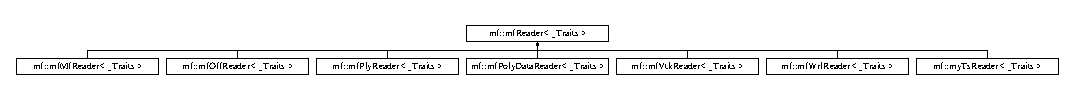
\includegraphics[height=0.776699cm]{classmf_1_1mfReader}
\end{center}
\end{figure}
\subsection*{Public Types}
\begin{DoxyCompactItemize}
\item 
\hypertarget{classmf_1_1mfReader_adbfe30c978c75ac98182d644b1b24752}{
typedef \_\-Traits::sMesh {\bfseries sMesh}}
\label{classmf_1_1mfReader_adbfe30c978c75ac98182d644b1b24752}

\end{DoxyCompactItemize}
\subsection*{Public Member Functions}
\begin{DoxyCompactItemize}
\item 
\hyperlink{classmf_1_1mfReader_a89a276eec0dbdb75a7985f894008959b}{mfReader} ()
\item 
virtual \hyperlink{classmf_1_1mfReader_ab0000ca6770e8bff2ea46fec0fb8b83e}{$\sim$mfReader} ()
\item 
virtual bool \hyperlink{classmf_1_1mfReader_a0e0c3224a06b06a8fb82be4f0f4a2e00}{read} (sMesh $\ast$malha, const char $\ast$filename)=0
\begin{DoxyCompactList}\small\item\em Executa a leitura de um arquivo. \item\end{DoxyCompactList}\end{DoxyCompactItemize}


\subsection{Detailed Description}
\subsubsection*{template$<$class \_\-Traits$>$ class mf::mfReader$<$ \_\-Traits $>$}

Modelo dos leitores de arquivos. Esta classe eh abstrata, devendo servir apenas de molde para novas implementacoes de leitores de arquivos. 

\subsection{Constructor \& Destructor Documentation}
\hypertarget{classmf_1_1mfReader_a89a276eec0dbdb75a7985f894008959b}{
\index{mf::mfReader@{mf::mfReader}!mfReader@{mfReader}}
\index{mfReader@{mfReader}!mf::mfReader@{mf::mfReader}}
\subsubsection[{mfReader}]{\setlength{\rightskip}{0pt plus 5cm}template$<$class \_\-Traits $>$ {\bf mf::mfReader}$<$ \_\-Traits $>$::{\bf mfReader} (
\begin{DoxyParamCaption}
{}
\end{DoxyParamCaption}
)}}
\label{classmf_1_1mfReader_a89a276eec0dbdb75a7985f894008959b}
Construtor \hypertarget{classmf_1_1mfReader_ab0000ca6770e8bff2ea46fec0fb8b83e}{
\index{mf::mfReader@{mf::mfReader}!$\sim$mfReader@{$\sim$mfReader}}
\index{$\sim$mfReader@{$\sim$mfReader}!mf::mfReader@{mf::mfReader}}
\subsubsection[{$\sim$mfReader}]{\setlength{\rightskip}{0pt plus 5cm}template$<$class \_\-Traits $>$ {\bf mf::mfReader}$<$ \_\-Traits $>$::$\sim${\bf mfReader} (
\begin{DoxyParamCaption}
{}
\end{DoxyParamCaption}
)\hspace{0.3cm}{\ttfamily  \mbox{[}virtual\mbox{]}}}}
\label{classmf_1_1mfReader_ab0000ca6770e8bff2ea46fec0fb8b83e}
Destrutor 

\subsection{Member Function Documentation}
\hypertarget{classmf_1_1mfReader_a0e0c3224a06b06a8fb82be4f0f4a2e00}{
\index{mf::mfReader@{mf::mfReader}!read@{read}}
\index{read@{read}!mf::mfReader@{mf::mfReader}}
\subsubsection[{read}]{\setlength{\rightskip}{0pt plus 5cm}template$<$class \_\-Traits $>$ virtual bool {\bf mf::mfReader}$<$ \_\-Traits $>$::read (
\begin{DoxyParamCaption}
\item[{sMesh $\ast$}]{malha, }
\item[{const char $\ast$}]{filename}
\end{DoxyParamCaption}
)\hspace{0.3cm}{\ttfamily  \mbox{[}pure virtual\mbox{]}}}}
\label{classmf_1_1mfReader_a0e0c3224a06b06a8fb82be4f0f4a2e00}


Executa a leitura de um arquivo. 

Paraetros de entrada: malha : endereco de memoria de destino da malha a ser carregada. Ja deve estar alocado. filename : nome do arquivo da malha. 

Implemented in \hyperlink{classmf_1_1mfMfReader_a9e43439ba77d2afb25839f3ed4fb774f}{mf::mfMfReader$<$ \_\-Traits $>$}, \hyperlink{classmf_1_1mfOffReader_a40cf7f39c327b60827a5858dd3ec8ec9}{mf::mfOffReader$<$ \_\-Traits $>$}, \hyperlink{classmf_1_1mfPlyReader_ad4aa817979acdfdc6570d2badb288bda}{mf::mfPlyReader$<$ \_\-Traits $>$}, \hyperlink{classmf_1_1mfPolyDataReader_a2c013ff82158ddc91ab451257a3051d0}{mf::mfPolyDataReader$<$ \_\-Traits $>$}, \hyperlink{classmf_1_1mfVtkReader_a3cbb607039dd5acf5aa0071f8ee49786}{mf::mfVtkReader$<$ \_\-Traits $>$}, \hyperlink{classmf_1_1mfWrlReader_a1d4c505e8e62204674aba4a36d47751e}{mf::mfWrlReader$<$ \_\-Traits $>$}, and \hyperlink{classmf_1_1myTsReader_a84fa0feda9979c77cfb609f3310fd31e}{mf::myTsReader$<$ \_\-Traits $>$}.



The documentation for this class was generated from the following file:\begin{DoxyCompactItemize}
\item 
mfReader.h\end{DoxyCompactItemize}

\hypertarget{classmf_1_1mfSearchDIDO}{
\section{mf::mfSearchDIDO$<$ \_\-Traits $>$ Class Template Reference}
\label{classmf_1_1mfSearchDIDO}\index{mf::mfSearchDIDO@{mf::mfSearchDIDO}}
}
\subsection*{Public Types}
\begin{DoxyCompactItemize}
\item 
typedef \_\-Traits::sVertex \hyperlink{classmf_1_1mfSearchDIDO_ad6074a0d2b1cdc485e8e2f80e6919156}{sVertex}
\item 
typedef \_\-Traits::sCell \hyperlink{classmf_1_1mfSearchDIDO_a1dcd18812432c1b5bd738f1f1a9eaf5a}{sCell}
\item 
typedef \_\-Traits::ids \hyperlink{classmf_1_1mfSearchDIDO_a01104ce1f89f6f20c744a1b0f986a312}{ids}
\item 
typedef \_\-Traits::space \hyperlink{classmf_1_1mfSearchDIDO_a47bbf10b71c54f3e87032850c8cfe217}{space}
\item 
typedef \_\-Traits::sGeometric \hyperlink{classmf_1_1mfSearchDIDO_ad8d6f59a3f5c291249ea4e7905b543a1}{sGeometric}
\item 
typedef \_\-Traits::sMesh \hyperlink{classmf_1_1mfSearchDIDO_af73c732f3c0a7fe85765bb4c49bd5545}{sMesh}
\end{DoxyCompactItemize}
\subsection*{Public Member Functions}
\begin{DoxyCompactItemize}
\item 
\hyperlink{classmf_1_1mfSearchDIDO_a753f67ea994ce478a602d6b7eac3c537}{mfSearchDIDO} (\hyperlink{classmf_1_1mfSearchDIDO_af73c732f3c0a7fe85765bb4c49bd5545}{sMesh} $\ast$\_\-mesh)
\item 
\hyperlink{classmf_1_1mfSearchDIDO_adc4cffff1004acf0f73a06e64c22b9e4}{$\sim$mfSearchDIDO} ()
\item 
\hypertarget{classmf_1_1mfSearchDIDO_ac911d0b101d98ddfc5d2e078d9bfaed6}{
int {\bfseries dido} (\hyperlink{classmf_1_1mfSearchDIDO_ad6074a0d2b1cdc485e8e2f80e6919156}{sVertex} $\ast$\_\-v, \hyperlink{classmf_1_1mfSearchDIDO_a47bbf10b71c54f3e87032850c8cfe217}{space} $\ast$coords, \hyperlink{classmf_1_1mfSearchDIDO_a01104ce1f89f6f20c744a1b0f986a312}{ids} \&idcelula, int \&lado)}
\label{classmf_1_1mfSearchDIDO_ac911d0b101d98ddfc5d2e078d9bfaed6}

\item 
void \hyperlink{classmf_1_1mfSearchDIDO_a855c47d8485ef2285bdb168d30685b70}{setMesh} (\hyperlink{classmf_1_1mfSearchDIDO_af73c732f3c0a7fe85765bb4c49bd5545}{sMesh} $\ast$\_\-mesh)
\end{DoxyCompactItemize}
\subsubsection*{template$<$class \_\-Traits$>$ class mf::mfSearchDIDO$<$ \_\-Traits $>$}



\subsection{Member Typedef Documentation}
\hypertarget{classmf_1_1mfSearchDIDO_a01104ce1f89f6f20c744a1b0f986a312}{
\index{mf::mfSearchDIDO@{mf::mfSearchDIDO}!ids@{ids}}
\index{ids@{ids}!mf::mfSearchDIDO@{mf::mfSearchDIDO}}
\subsubsection[{ids}]{\setlength{\rightskip}{0pt plus 5cm}template$<$class \_\-Traits $>$ typedef \_\-Traits::ids {\bf mf::mfSearchDIDO}$<$ \_\-Traits $>$::{\bf ids}}}
\label{classmf_1_1mfSearchDIDO_a01104ce1f89f6f20c744a1b0f986a312}
Id typename definition \hypertarget{classmf_1_1mfSearchDIDO_a1dcd18812432c1b5bd738f1f1a9eaf5a}{
\index{mf::mfSearchDIDO@{mf::mfSearchDIDO}!sCell@{sCell}}
\index{sCell@{sCell}!mf::mfSearchDIDO@{mf::mfSearchDIDO}}
\subsubsection[{sCell}]{\setlength{\rightskip}{0pt plus 5cm}template$<$class \_\-Traits $>$ typedef \_\-Traits::sCell {\bf mf::mfSearchDIDO}$<$ \_\-Traits $>$::{\bf sCell}}}
\label{classmf_1_1mfSearchDIDO_a1dcd18812432c1b5bd738f1f1a9eaf5a}
Cell typename definition \hypertarget{classmf_1_1mfSearchDIDO_ad8d6f59a3f5c291249ea4e7905b543a1}{
\index{mf::mfSearchDIDO@{mf::mfSearchDIDO}!sGeometric@{sGeometric}}
\index{sGeometric@{sGeometric}!mf::mfSearchDIDO@{mf::mfSearchDIDO}}
\subsubsection[{sGeometric}]{\setlength{\rightskip}{0pt plus 5cm}template$<$class \_\-Traits $>$ typedef \_\-Traits::sGeometric {\bf mf::mfSearchDIDO}$<$ \_\-Traits $>$::{\bf sGeometric}}}
\label{classmf_1_1mfSearchDIDO_ad8d6f59a3f5c291249ea4e7905b543a1}
Geometric typename definition \hypertarget{classmf_1_1mfSearchDIDO_af73c732f3c0a7fe85765bb4c49bd5545}{
\index{mf::mfSearchDIDO@{mf::mfSearchDIDO}!sMesh@{sMesh}}
\index{sMesh@{sMesh}!mf::mfSearchDIDO@{mf::mfSearchDIDO}}
\subsubsection[{sMesh}]{\setlength{\rightskip}{0pt plus 5cm}template$<$class \_\-Traits $>$ typedef \_\-Traits::sMesh {\bf mf::mfSearchDIDO}$<$ \_\-Traits $>$::{\bf sMesh}}}
\label{classmf_1_1mfSearchDIDO_af73c732f3c0a7fe85765bb4c49bd5545}
Mesh typename definition \hypertarget{classmf_1_1mfSearchDIDO_a47bbf10b71c54f3e87032850c8cfe217}{
\index{mf::mfSearchDIDO@{mf::mfSearchDIDO}!space@{space}}
\index{space@{space}!mf::mfSearchDIDO@{mf::mfSearchDIDO}}
\subsubsection[{space}]{\setlength{\rightskip}{0pt plus 5cm}template$<$class \_\-Traits $>$ typedef \_\-Traits::space {\bf mf::mfSearchDIDO}$<$ \_\-Traits $>$::{\bf space}}}
\label{classmf_1_1mfSearchDIDO_a47bbf10b71c54f3e87032850c8cfe217}
Space typename definition \hypertarget{classmf_1_1mfSearchDIDO_ad6074a0d2b1cdc485e8e2f80e6919156}{
\index{mf::mfSearchDIDO@{mf::mfSearchDIDO}!sVertex@{sVertex}}
\index{sVertex@{sVertex}!mf::mfSearchDIDO@{mf::mfSearchDIDO}}
\subsubsection[{sVertex}]{\setlength{\rightskip}{0pt plus 5cm}template$<$class \_\-Traits $>$ typedef \_\-Traits::sVertex {\bf mf::mfSearchDIDO}$<$ \_\-Traits $>$::{\bf sVertex}}}
\label{classmf_1_1mfSearchDIDO_ad6074a0d2b1cdc485e8e2f80e6919156}
Vertex typename definition 

\subsection{Constructor \& Destructor Documentation}
\hypertarget{classmf_1_1mfSearchDIDO_a753f67ea994ce478a602d6b7eac3c537}{
\index{mf::mfSearchDIDO@{mf::mfSearchDIDO}!mfSearchDIDO@{mfSearchDIDO}}
\index{mfSearchDIDO@{mfSearchDIDO}!mf::mfSearchDIDO@{mf::mfSearchDIDO}}
\subsubsection[{mfSearchDIDO}]{\setlength{\rightskip}{0pt plus 5cm}template$<$class \_\-Traits $>$ {\bf mf::mfSearchDIDO}$<$ \_\-Traits $>$::{\bf mfSearchDIDO} (
\begin{DoxyParamCaption}
\item[{{\bf sMesh} $\ast$}]{\_\-mesh}
\end{DoxyParamCaption}
)}}
\label{classmf_1_1mfSearchDIDO_a753f67ea994ce478a602d6b7eac3c537}
Construtor


\begin{DoxyParams}{Parameters}
{\em \_\-mesh,:} & the mesh address that this class will manipulate \\
\hline
\end{DoxyParams}
\hypertarget{classmf_1_1mfSearchDIDO_adc4cffff1004acf0f73a06e64c22b9e4}{
\index{mf::mfSearchDIDO@{mf::mfSearchDIDO}!$\sim$mfSearchDIDO@{$\sim$mfSearchDIDO}}
\index{$\sim$mfSearchDIDO@{$\sim$mfSearchDIDO}!mf::mfSearchDIDO@{mf::mfSearchDIDO}}
\subsubsection[{$\sim$mfSearchDIDO}]{\setlength{\rightskip}{0pt plus 5cm}template$<$class \_\-Traits $>$ {\bf mf::mfSearchDIDO}$<$ \_\-Traits $>$::$\sim${\bf mfSearchDIDO} (
\begin{DoxyParamCaption}
{}
\end{DoxyParamCaption}
)}}
\label{classmf_1_1mfSearchDIDO_adc4cffff1004acf0f73a06e64c22b9e4}
Destrutor 

\subsection{Member Function Documentation}
\hypertarget{classmf_1_1mfSearchDIDO_a855c47d8485ef2285bdb168d30685b70}{
\index{mf::mfSearchDIDO@{mf::mfSearchDIDO}!setMesh@{setMesh}}
\index{setMesh@{setMesh}!mf::mfSearchDIDO@{mf::mfSearchDIDO}}
\subsubsection[{setMesh}]{\setlength{\rightskip}{0pt plus 5cm}template$<$class \_\-Traits $>$ void {\bf mf::mfSearchDIDO}$<$ \_\-Traits $>$::setMesh (
\begin{DoxyParamCaption}
\item[{{\bf sMesh} $\ast$}]{\_\-mesh}
\end{DoxyParamCaption}
)}}
\label{classmf_1_1mfSearchDIDO_a855c47d8485ef2285bdb168d30685b70}
Set the mesh instance to which this class will manipulate.


\begin{DoxyParams}{Parameters}
{\em \_\-mesh,:} & the mesh address that this class will manipulate \\
\hline
\end{DoxyParams}


The documentation for this class was generated from the following file:\begin{DoxyCompactItemize}
\item 
mfSearchDIDO.h\end{DoxyCompactItemize}

\hypertarget{classmf_1_1mfSing}{
\section{mf::mfSing$<$ \_\-Traits $>$ Class Template Reference}
\label{classmf_1_1mfSing}\index{mf::mfSing@{mf::mfSing}}
}
\subsection*{Public Types}
\begin{DoxyCompactItemize}
\item 
typedef \_\-Traits::ids \hyperlink{classmf_1_1mfSing_a2b7b2246fabd10500aa23792900ffa5a}{ids}
\item 
typedef \hyperlink{classmf_1_1mfSing}{mfSing}$<$ \_\-Traits $>$ \hyperlink{classmf_1_1mfSing_a06d61023a91b916dd86e6a56a62dcbb2}{sSing}
\end{DoxyCompactItemize}
\subsection*{Public Member Functions}
\begin{DoxyCompactItemize}
\item 
\hyperlink{classmf_1_1mfSing_a1d88a4a40e1a978e8b42b1944f8ab5ad}{mfSing} ()
\item 
\hyperlink{classmf_1_1mfSing_acfc045aa59c8dde458b3bc4ca3077ac5}{$\sim$mfSing} ()
\item 
\hyperlink{classmf_1_1mfSing}{sSing} $\ast$ \hyperlink{classmf_1_1mfSing_aeccff777fb1a65aed98f35d20ba8b3c8}{getNext} ()
\item 
void \hyperlink{classmf_1_1mfSing_a06575423647881c2a37a960531b587ba}{setNext} (\hyperlink{classmf_1_1mfSing}{sSing} $\ast$\_\-next)
\item 
\hyperlink{classmf_1_1mfSing_a2b7b2246fabd10500aa23792900ffa5a}{ids} \hyperlink{classmf_1_1mfSing_a80d7f9eb1dadc79d0119786ef9aabce8}{getCell} ()
\item 
void \hyperlink{classmf_1_1mfSing_adee93728a924425fd113d286abfa52dd}{setCell} (\hyperlink{classmf_1_1mfSing_a2b7b2246fabd10500aa23792900ffa5a}{ids} \_\-cell)
\end{DoxyCompactItemize}
\subsubsection*{template$<$class \_\-Traits$>$ class mf::mfSing$<$ \_\-Traits $>$}



\subsection{Member Typedef Documentation}
\hypertarget{classmf_1_1mfSing_a2b7b2246fabd10500aa23792900ffa5a}{
\index{mf::mfSing@{mf::mfSing}!ids@{ids}}
\index{ids@{ids}!mf::mfSing@{mf::mfSing}}
\subsubsection[{ids}]{\setlength{\rightskip}{0pt plus 5cm}template$<$class \_\-Traits $>$ typedef \_\-Traits::ids {\bf mf::mfSing}$<$ \_\-Traits $>$::{\bf ids}}}
\label{classmf_1_1mfSing_a2b7b2246fabd10500aa23792900ffa5a}
Id typename definition \hypertarget{classmf_1_1mfSing_a06d61023a91b916dd86e6a56a62dcbb2}{
\index{mf::mfSing@{mf::mfSing}!sSing@{sSing}}
\index{sSing@{sSing}!mf::mfSing@{mf::mfSing}}
\subsubsection[{sSing}]{\setlength{\rightskip}{0pt plus 5cm}template$<$class \_\-Traits $>$ typedef {\bf mfSing}$<$\_\-Traits$>$ {\bf mf::mfSing}$<$ \_\-Traits $>$::{\bf sSing}}}
\label{classmf_1_1mfSing_a06d61023a91b916dd86e6a56a62dcbb2}
Singular typename definition 

\subsection{Constructor \& Destructor Documentation}
\hypertarget{classmf_1_1mfSing_a1d88a4a40e1a978e8b42b1944f8ab5ad}{
\index{mf::mfSing@{mf::mfSing}!mfSing@{mfSing}}
\index{mfSing@{mfSing}!mf::mfSing@{mf::mfSing}}
\subsubsection[{mfSing}]{\setlength{\rightskip}{0pt plus 5cm}template$<$class \_\-Traits $>$ {\bf mf::mfSing}$<$ \_\-Traits $>$::{\bf mfSing} (
\begin{DoxyParamCaption}
{}
\end{DoxyParamCaption}
)}}
\label{classmf_1_1mfSing_a1d88a4a40e1a978e8b42b1944f8ab5ad}
Constructor \hypertarget{classmf_1_1mfSing_acfc045aa59c8dde458b3bc4ca3077ac5}{
\index{mf::mfSing@{mf::mfSing}!$\sim$mfSing@{$\sim$mfSing}}
\index{$\sim$mfSing@{$\sim$mfSing}!mf::mfSing@{mf::mfSing}}
\subsubsection[{$\sim$mfSing}]{\setlength{\rightskip}{0pt plus 5cm}template$<$class \_\-Traits $>$ {\bf mf::mfSing}$<$ \_\-Traits $>$::$\sim${\bf mfSing} (
\begin{DoxyParamCaption}
{}
\end{DoxyParamCaption}
)}}
\label{classmf_1_1mfSing_acfc045aa59c8dde458b3bc4ca3077ac5}
Destrutor 

\subsection{Member Function Documentation}
\hypertarget{classmf_1_1mfSing_a80d7f9eb1dadc79d0119786ef9aabce8}{
\index{mf::mfSing@{mf::mfSing}!getCell@{getCell}}
\index{getCell@{getCell}!mf::mfSing@{mf::mfSing}}
\subsubsection[{getCell}]{\setlength{\rightskip}{0pt plus 5cm}template$<$class \_\-Traits $>$ IDS {\bf mf::mfSing}$<$ \_\-Traits $>$::getCell (
\begin{DoxyParamCaption}
{}
\end{DoxyParamCaption}
)}}
\label{classmf_1_1mfSing_a80d7f9eb1dadc79d0119786ef9aabce8}
Return the cell of this singular component

\begin{DoxyReturn}{Returns}
ID of the cell of the singular component 
\end{DoxyReturn}
\hypertarget{classmf_1_1mfSing_aeccff777fb1a65aed98f35d20ba8b3c8}{
\index{mf::mfSing@{mf::mfSing}!getNext@{getNext}}
\index{getNext@{getNext}!mf::mfSing@{mf::mfSing}}
\subsubsection[{getNext}]{\setlength{\rightskip}{0pt plus 5cm}template$<$class \_\-Traits $>$ SSING $\ast$ {\bf mf::mfSing}$<$ \_\-Traits $>$::getNext (
\begin{DoxyParamCaption}
{}
\end{DoxyParamCaption}
)}}
\label{classmf_1_1mfSing_aeccff777fb1a65aed98f35d20ba8b3c8}
Return the next singular component

\begin{DoxyReturn}{Returns}
Instance of the next singular component 
\end{DoxyReturn}
\hypertarget{classmf_1_1mfSing_adee93728a924425fd113d286abfa52dd}{
\index{mf::mfSing@{mf::mfSing}!setCell@{setCell}}
\index{setCell@{setCell}!mf::mfSing@{mf::mfSing}}
\subsubsection[{setCell}]{\setlength{\rightskip}{0pt plus 5cm}template$<$class \_\-Traits $>$ void {\bf mf::mfSing}$<$ \_\-Traits $>$::setCell (
\begin{DoxyParamCaption}
\item[{{\bf ids}}]{\_\-cell}
\end{DoxyParamCaption}
)}}
\label{classmf_1_1mfSing_adee93728a924425fd113d286abfa52dd}
Define the cell of this singular component


\begin{DoxyParams}{Parameters}
{\em cell,:} & ID of the cell of the singular component \\
\hline
\end{DoxyParams}
\hypertarget{classmf_1_1mfSing_a06575423647881c2a37a960531b587ba}{
\index{mf::mfSing@{mf::mfSing}!setNext@{setNext}}
\index{setNext@{setNext}!mf::mfSing@{mf::mfSing}}
\subsubsection[{setNext}]{\setlength{\rightskip}{0pt plus 5cm}template$<$class \_\-Traits $>$ void {\bf mf::mfSing}$<$ \_\-Traits $>$::setNext (
\begin{DoxyParamCaption}
\item[{{\bf sSing} $\ast$}]{\_\-next}
\end{DoxyParamCaption}
)}}
\label{classmf_1_1mfSing_a06575423647881c2a37a960531b587ba}
Define the next singular component


\begin{DoxyParams}{Parameters}
{\em next,:} & the next component on the singular list \\
\hline
\end{DoxyParams}


The documentation for this class was generated from the following file:\begin{DoxyCompactItemize}
\item 
\hyperlink{mfSing_8h}{mfSing.h}\end{DoxyCompactItemize}

\hypertarget{classmf_1_1mfSingularVertex}{
\section{mf::mfSingularVertex$<$ size, \_\-Traits $>$ Class Template Reference}
\label{classmf_1_1mfSingularVertex}\index{mf::mfSingularVertex@{mf::mfSingularVertex}}
}


{\ttfamily \#include $<$mfSingularVertex.h$>$}

Inheritance diagram for mf::mfSingularVertex$<$ size, \_\-Traits $>$:\begin{figure}[H]
\begin{center}
\leavevmode
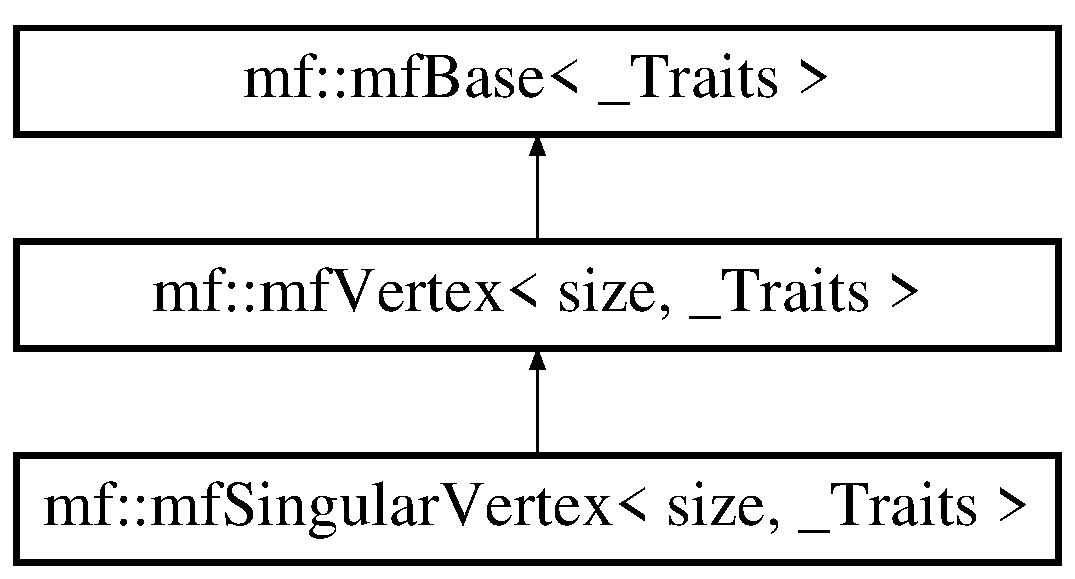
\includegraphics[height=3.000000cm]{classmf_1_1mfSingularVertex}
\end{center}
\end{figure}
\subsection*{Public Types}
\begin{DoxyCompactItemize}
\item 
typedef \_\-Traits::ids \hyperlink{classmf_1_1mfSingularVertex_ad951601375961980e2ad033de57e14a1}{ids}
\item 
typedef \_\-Traits::space \hyperlink{classmf_1_1mfSingularVertex_a96d4909dd62a8e8889eda76d0148db2a}{space}
\item 
typedef \hyperlink{classmf_1_1mfSing}{mfSing}$<$ \_\-Traits $>$ \hyperlink{classmf_1_1mfSingularVertex_ac992cd55c8554406174a3a1449af209b}{sSing}
\end{DoxyCompactItemize}
\subsection*{Public Member Functions}
\begin{DoxyCompactItemize}
\item 
\hyperlink{classmf_1_1mfSingularVertex_a44c61e349c686e1ffeaec3f6bbe5010c}{mfSingularVertex} ()
\item 
\hyperlink{classmf_1_1mfSingularVertex_a8f9efd5ee656e83a0f50c9833fc2af9f}{$\sim$mfSingularVertex} ()
\item 
bool \hyperlink{classmf_1_1mfSingularVertex_a2a85f3a4a1b98b63ca9504ef1ad4da7e}{isSingular} (MF\_\-DMUTEXD)
\item 
int \hyperlink{classmf_1_1mfSingularVertex_a5256ee7412e6d5173390fc7409d74fc5}{getNumberOfSings} (MF\_\-DMUTEXD)
\item 
\hyperlink{classmf_1_1mfBase_a3b23f16ddf59da0a91ab12cf57c1f111}{ids} \hyperlink{classmf_1_1mfSingularVertex_a3614e72d2adb6efef5345ef0edf30c47}{getSingCell} (int pos=0 MF\_\-DMUTEXVD)
\item 
bool \hyperlink{classmf_1_1mfSingularVertex_a943c961054aaf8e3512254ea8312640a}{setSingCell} (int pos, \hyperlink{classmf_1_1mfBase_a3b23f16ddf59da0a91ab12cf57c1f111}{ids} cell MF\_\-DMUTEXVD)
\item 
int \hyperlink{classmf_1_1mfSingularVertex_a8100c3e3601205ca8996057cc0732b1a}{addSing} (\hyperlink{classmf_1_1mfBase_a3b23f16ddf59da0a91ab12cf57c1f111}{ids} cell MF\_\-DMUTEXVD)
\item 
bool \hyperlink{classmf_1_1mfSingularVertex_a2e7093fbc051f93cf99c092ff8dcfa70}{delSing} (int pos MF\_\-DMUTEXVD)
\item 
void \hyperlink{classmf_1_1mfSingularVertex_a86f55d574e4415c530d7945018802da3}{clearSings} (MF\_\-DMUTEXD)
\item 
int \hyperlink{classmf_1_1mfSingularVertex_a834794974d9a2a6315830da23abf3378}{inSings} (\hyperlink{classmf_1_1mfBase_a3b23f16ddf59da0a91ab12cf57c1f111}{ids} cell MF\_\-DMUTEXVD)
\item 
\hyperlink{classmf_1_1mfSing}{sSing} $\ast$ \hyperlink{classmf_1_1mfSingularVertex_adc2be2ffb1b40b539ce0bbff34aa1a99}{getSing} (MF\_\-DMUTEXD)
\end{DoxyCompactItemize}


\subsection{Detailed Description}
\subsubsection*{template$<$int size, class \_\-Traits$>$ class mf::mfSingularVertex$<$ size, \_\-Traits $>$}

Base class of singular vertex

\_\-Traits must have typenames: ids, space, sSing

/$\ast$$\ast$ 

\subsection{Member Typedef Documentation}
\hypertarget{classmf_1_1mfSingularVertex_ad951601375961980e2ad033de57e14a1}{
\index{mf::mfSingularVertex@{mf::mfSingularVertex}!ids@{ids}}
\index{ids@{ids}!mf::mfSingularVertex@{mf::mfSingularVertex}}
\subsubsection[{ids}]{\setlength{\rightskip}{0pt plus 5cm}template$<$int size, class \_\-Traits$>$ typedef \_\-Traits::ids {\bf mf::mfSingularVertex}$<$ size, \_\-Traits $>$::{\bf ids}}}
\label{classmf_1_1mfSingularVertex_ad951601375961980e2ad033de57e14a1}
Id typename definition 

Reimplemented from \hyperlink{classmf_1_1mfBase_a3b23f16ddf59da0a91ab12cf57c1f111}{mf::mfBase$<$ \_\-Traits $>$}.

\hypertarget{classmf_1_1mfSingularVertex_a96d4909dd62a8e8889eda76d0148db2a}{
\index{mf::mfSingularVertex@{mf::mfSingularVertex}!space@{space}}
\index{space@{space}!mf::mfSingularVertex@{mf::mfSingularVertex}}
\subsubsection[{space}]{\setlength{\rightskip}{0pt plus 5cm}template$<$int size, class \_\-Traits$>$ typedef \_\-Traits::space {\bf mf::mfSingularVertex}$<$ size, \_\-Traits $>$::{\bf space}}}
\label{classmf_1_1mfSingularVertex_a96d4909dd62a8e8889eda76d0148db2a}
Space typename definition 

Reimplemented from \hyperlink{classmf_1_1mfVertex_a9710b0b7ac7bbb276e1e97d541cbfc93}{mf::mfVertex$<$ size, \_\-Traits $>$}.



Reimplemented in \hyperlink{classmf_1_1mfVertex2D_a0730a219bea43b0b049cae2b4c72527b}{mf::mfVertex2D$<$ \_\-Traits $>$}, and \hyperlink{classmf_1_1mfVertex3D_a16aa06a4ca21fae048fa56b7a40ac088}{mf::mfVertex3D$<$ \_\-Traits $>$}.

\hypertarget{classmf_1_1mfSingularVertex_ac992cd55c8554406174a3a1449af209b}{
\index{mf::mfSingularVertex@{mf::mfSingularVertex}!sSing@{sSing}}
\index{sSing@{sSing}!mf::mfSingularVertex@{mf::mfSingularVertex}}
\subsubsection[{sSing}]{\setlength{\rightskip}{0pt plus 5cm}template$<$int size, class \_\-Traits$>$ typedef {\bf mfSing}$<$\_\-Traits$>$ {\bf mf::mfSingularVertex}$<$ size, \_\-Traits $>$::{\bf sSing}}}
\label{classmf_1_1mfSingularVertex_ac992cd55c8554406174a3a1449af209b}
Singular typename definition 

\subsection{Constructor \& Destructor Documentation}
\hypertarget{classmf_1_1mfSingularVertex_a44c61e349c686e1ffeaec3f6bbe5010c}{
\index{mf::mfSingularVertex@{mf::mfSingularVertex}!mfSingularVertex@{mfSingularVertex}}
\index{mfSingularVertex@{mfSingularVertex}!mf::mfSingularVertex@{mf::mfSingularVertex}}
\subsubsection[{mfSingularVertex}]{\setlength{\rightskip}{0pt plus 5cm}template$<$int size, class \_\-Traits $>$ {\bf mf::mfSingularVertex}$<$ size, \_\-Traits $>$::{\bf mfSingularVertex} (
\begin{DoxyParamCaption}
{}
\end{DoxyParamCaption}
)}}
\label{classmf_1_1mfSingularVertex_a44c61e349c686e1ffeaec3f6bbe5010c}
Constructor \hypertarget{classmf_1_1mfSingularVertex_a8f9efd5ee656e83a0f50c9833fc2af9f}{
\index{mf::mfSingularVertex@{mf::mfSingularVertex}!$\sim$mfSingularVertex@{$\sim$mfSingularVertex}}
\index{$\sim$mfSingularVertex@{$\sim$mfSingularVertex}!mf::mfSingularVertex@{mf::mfSingularVertex}}
\subsubsection[{$\sim$mfSingularVertex}]{\setlength{\rightskip}{0pt plus 5cm}template$<$int size, class \_\-Traits $>$ {\bf mf::mfSingularVertex}$<$ size, \_\-Traits $>$::$\sim${\bf mfSingularVertex} (
\begin{DoxyParamCaption}
{}
\end{DoxyParamCaption}
)}}
\label{classmf_1_1mfSingularVertex_a8f9efd5ee656e83a0f50c9833fc2af9f}
Destructor 

\subsection{Member Function Documentation}
\hypertarget{classmf_1_1mfSingularVertex_a8100c3e3601205ca8996057cc0732b1a}{
\index{mf::mfSingularVertex@{mf::mfSingularVertex}!addSing@{addSing}}
\index{addSing@{addSing}!mf::mfSingularVertex@{mf::mfSingularVertex}}
\subsubsection[{addSing}]{\setlength{\rightskip}{0pt plus 5cm}template$<$int size, class \_\-Traits $>$ int {\bf mf::mfSingularVertex}$<$ size, \_\-Traits $>$::addSing (
\begin{DoxyParamCaption}
\item[{{\bf ids} cell}]{MF\_\-DMUTEXVD}
\end{DoxyParamCaption}
)}}
\label{classmf_1_1mfSingularVertex_a8100c3e3601205ca8996057cc0732b1a}
Add a singular component


\begin{DoxyParams}{Parameters}
{\em cell,:} & cell to be add \\
\hline
\end{DoxyParams}
\begin{DoxyReturn}{Returns}
index of added singular component 
\end{DoxyReturn}
\hypertarget{classmf_1_1mfSingularVertex_a86f55d574e4415c530d7945018802da3}{
\index{mf::mfSingularVertex@{mf::mfSingularVertex}!clearSings@{clearSings}}
\index{clearSings@{clearSings}!mf::mfSingularVertex@{mf::mfSingularVertex}}
\subsubsection[{clearSings}]{\setlength{\rightskip}{0pt plus 5cm}template$<$int size, class \_\-Traits$>$ void {\bf mf::mfSingularVertex}$<$ size, \_\-Traits $>$::clearSings (
\begin{DoxyParamCaption}
\item[{MF\_\-DMUTEXD}]{}
\end{DoxyParamCaption}
)}}
\label{classmf_1_1mfSingularVertex_a86f55d574e4415c530d7945018802da3}
Delete all singular components \hypertarget{classmf_1_1mfSingularVertex_a2e7093fbc051f93cf99c092ff8dcfa70}{
\index{mf::mfSingularVertex@{mf::mfSingularVertex}!delSing@{delSing}}
\index{delSing@{delSing}!mf::mfSingularVertex@{mf::mfSingularVertex}}
\subsubsection[{delSing}]{\setlength{\rightskip}{0pt plus 5cm}template$<$int size, class \_\-Traits $>$ bool {\bf mf::mfSingularVertex}$<$ size, \_\-Traits $>$::delSing (
\begin{DoxyParamCaption}
\item[{int pos}]{MF\_\-DMUTEXVD}
\end{DoxyParamCaption}
)}}
\label{classmf_1_1mfSingularVertex_a2e7093fbc051f93cf99c092ff8dcfa70}
Delete a singular component


\begin{DoxyParams}{Parameters}
{\em pos,:} & index of singular component \\
\hline
\end{DoxyParams}
\begin{DoxyReturn}{Returns}
true if successful 
\end{DoxyReturn}
\hypertarget{classmf_1_1mfSingularVertex_a5256ee7412e6d5173390fc7409d74fc5}{
\index{mf::mfSingularVertex@{mf::mfSingularVertex}!getNumberOfSings@{getNumberOfSings}}
\index{getNumberOfSings@{getNumberOfSings}!mf::mfSingularVertex@{mf::mfSingularVertex}}
\subsubsection[{getNumberOfSings}]{\setlength{\rightskip}{0pt plus 5cm}template$<$int size, class \_\-Traits$>$ int {\bf mf::mfSingularVertex}$<$ size, \_\-Traits $>$::getNumberOfSings (
\begin{DoxyParamCaption}
\item[{MF\_\-DMUTEXD}]{}
\end{DoxyParamCaption}
)}}
\label{classmf_1_1mfSingularVertex_a5256ee7412e6d5173390fc7409d74fc5}
Return the number of sSing (number of singular components) \hypertarget{classmf_1_1mfSingularVertex_adc2be2ffb1b40b539ce0bbff34aa1a99}{
\index{mf::mfSingularVertex@{mf::mfSingularVertex}!getSing@{getSing}}
\index{getSing@{getSing}!mf::mfSingularVertex@{mf::mfSingularVertex}}
\subsubsection[{getSing}]{\setlength{\rightskip}{0pt plus 5cm}template$<$int size, class \_\-Traits$>$ {\bf sSing}$\ast$ {\bf mf::mfSingularVertex}$<$ size, \_\-Traits $>$::getSing (
\begin{DoxyParamCaption}
\item[{MF\_\-DMUTEXD}]{}
\end{DoxyParamCaption}
)}}
\label{classmf_1_1mfSingularVertex_adc2be2ffb1b40b539ce0bbff34aa1a99}
Return the first singular component \hypertarget{classmf_1_1mfSingularVertex_a3614e72d2adb6efef5345ef0edf30c47}{
\index{mf::mfSingularVertex@{mf::mfSingularVertex}!getSingCell@{getSingCell}}
\index{getSingCell@{getSingCell}!mf::mfSingularVertex@{mf::mfSingularVertex}}
\subsubsection[{getSingCell}]{\setlength{\rightskip}{0pt plus 5cm}template$<$int size, class \_\-Traits $>$ IDS {\bf mf::mfSingularVertex}$<$ size, \_\-Traits $>$::getSingCell (
\begin{DoxyParamCaption}
\item[{int pos}]{MF\_\-DMUTEXV = {\ttfamily 0~MF\_\-DMUTEXVD}}
\end{DoxyParamCaption}
)}}
\label{classmf_1_1mfSingularVertex_a3614e72d2adb6efef5345ef0edf30c47}
Return the first cell of each singular component


\begin{DoxyParams}{Parameters}
{\em pos,:} & index of singular component \\
\hline
\end{DoxyParams}
\begin{DoxyReturn}{Returns}
one cell of 'pos' singular component 
\end{DoxyReturn}
\hypertarget{classmf_1_1mfSingularVertex_a834794974d9a2a6315830da23abf3378}{
\index{mf::mfSingularVertex@{mf::mfSingularVertex}!inSings@{inSings}}
\index{inSings@{inSings}!mf::mfSingularVertex@{mf::mfSingularVertex}}
\subsubsection[{inSings}]{\setlength{\rightskip}{0pt plus 5cm}template$<$int size, class \_\-Traits $>$ int {\bf mf::mfSingularVertex}$<$ size, \_\-Traits $>$::inSings (
\begin{DoxyParamCaption}
\item[{{\bf ids} cell}]{MF\_\-DMUTEXVD}
\end{DoxyParamCaption}
)}}
\label{classmf_1_1mfSingularVertex_a834794974d9a2a6315830da23abf3378}
Return the position of the specified cell in list of singular components \hypertarget{classmf_1_1mfSingularVertex_a2a85f3a4a1b98b63ca9504ef1ad4da7e}{
\index{mf::mfSingularVertex@{mf::mfSingularVertex}!isSingular@{isSingular}}
\index{isSingular@{isSingular}!mf::mfSingularVertex@{mf::mfSingularVertex}}
\subsubsection[{isSingular}]{\setlength{\rightskip}{0pt plus 5cm}template$<$int size, class \_\-Traits$>$ bool {\bf mf::mfSingularVertex}$<$ size, \_\-Traits $>$::isSingular (
\begin{DoxyParamCaption}
\item[{MF\_\-DMUTEXD}]{}
\end{DoxyParamCaption}
)}}
\label{classmf_1_1mfSingularVertex_a2a85f3a4a1b98b63ca9504ef1ad4da7e}
Return true if this vertex is singular \hypertarget{classmf_1_1mfSingularVertex_a943c961054aaf8e3512254ea8312640a}{
\index{mf::mfSingularVertex@{mf::mfSingularVertex}!setSingCell@{setSingCell}}
\index{setSingCell@{setSingCell}!mf::mfSingularVertex@{mf::mfSingularVertex}}
\subsubsection[{setSingCell}]{\setlength{\rightskip}{0pt plus 5cm}template$<$int size, class \_\-Traits $>$ bool {\bf mf::mfSingularVertex}$<$ size, \_\-Traits $>$::setSingCell (
\begin{DoxyParamCaption}
\item[{int}]{pos, }
\item[{{\bf ids} cell}]{MF\_\-DMUTEXVD}
\end{DoxyParamCaption}
)}}
\label{classmf_1_1mfSingularVertex_a943c961054aaf8e3512254ea8312640a}
Set a singular component


\begin{DoxyParams}{Parameters}
{\em pos,:} & index of singular component \\
\hline
{\em cell,:} & cell to be set \\
\hline
\end{DoxyParams}
\begin{DoxyReturn}{Returns}
true if 'pos' exist
\end{DoxyReturn}
For add a singular component use addSing 

The documentation for this class was generated from the following file:\begin{DoxyCompactItemize}
\item 
\hyperlink{mfSingularVertex_8h}{mfSingularVertex.h}\end{DoxyCompactItemize}

\hypertarget{classmf_1_1mfTetraCell}{
\section{mf::mfTetraCell$<$ \_\-Traits $>$ Class Template Reference}
\label{classmf_1_1mfTetraCell}\index{mf::mfTetraCell@{mf::mfTetraCell}}
}
Inheritance diagram for mf::mfTetraCell$<$ \_\-Traits $>$:\begin{figure}[H]
\begin{center}
\leavevmode
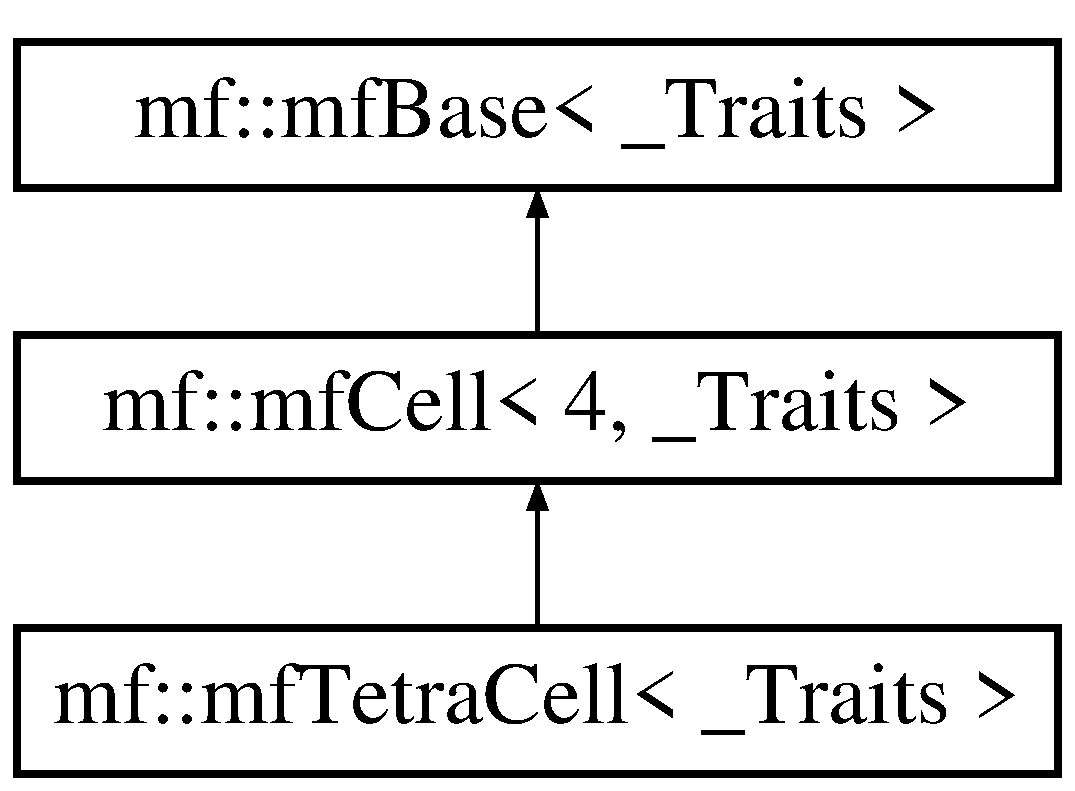
\includegraphics[height=3.000000cm]{classmf_1_1mfTetraCell}
\end{center}
\end{figure}
\subsection*{Public Types}
\begin{DoxyCompactItemize}
\item 
typedef \_\-Traits::ids \hyperlink{classmf_1_1mfTetraCell_a1fe27f9bfd856ec3464b2b671ceaf558}{ids}
\end{DoxyCompactItemize}
\subsection*{Public Member Functions}
\begin{DoxyCompactItemize}
\item 
\hyperlink{classmf_1_1mfTetraCell_a2e18ff7f38ded3a98cb44a44dc955fd5}{mfTetraCell} ()
\item 
virtual \hyperlink{classmf_1_1mfTetraCell_ae1a1b462e99342bf35614f1c09e1c630}{$\sim$mfTetraCell} ()
\item 
\hyperlink{classmf_1_1mfBase_a3b23f16ddf59da0a91ab12cf57c1f111}{ids} \hyperlink{classmf_1_1mfTetraCell_a3b34d618f13b889fd1dfa008bdd79541}{getEdgeId} (int index MF\_\-DMUTEXVD)
\item 
\hyperlink{classmf_1_1mfBase_a3b23f16ddf59da0a91ab12cf57c1f111}{ids} \hyperlink{classmf_1_1mfTetraCell_a946fd7394f718ef614076d3a15314b07}{getMateId} (int index MF\_\-DMUTEXVD)
\item 
void \hyperlink{classmf_1_1mfTetraCell_af6231dd16c5fb6e20aebd9f9127cd138}{setEdgeId} (int index, \hyperlink{classmf_1_1mfBase_a3b23f16ddf59da0a91ab12cf57c1f111}{ids} edge MF\_\-DMUTEXVD)
\item 
void \hyperlink{classmf_1_1mfTetraCell_acbe15a78f605cfbbc8f62acc3cf4bc0a}{setMateId} (int index, \hyperlink{classmf_1_1mfBase_a3b23f16ddf59da0a91ab12cf57c1f111}{ids} cell MF\_\-DMUTEXVD)
\item 
int \hyperlink{classmf_1_1mfTetraCell_a0a4f78f89482e6a45cbe2556cf8fa496}{getRightFaceIndex} (\hyperlink{classmf_1_1mfBase_a3b23f16ddf59da0a91ab12cf57c1f111}{ids} index1, \hyperlink{classmf_1_1mfBase_a3b23f16ddf59da0a91ab12cf57c1f111}{ids} index2)
\item 
int \hyperlink{classmf_1_1mfTetraCell_a2b8f436018c47313fbd98d6ef63e8d3d}{getLeftFaceIndex} (\hyperlink{classmf_1_1mfBase_a3b23f16ddf59da0a91ab12cf57c1f111}{ids} index1, \hyperlink{classmf_1_1mfBase_a3b23f16ddf59da0a91ab12cf57c1f111}{ids} index2)
\item 
void \hyperlink{classmf_1_1mfTetraCell_a9e553dc8c297b53756f44a9782facf5c}{clearMates} (MF\_\-DMUTEXD)
\item 
int \hyperlink{classmf_1_1mfTetraCell_a6fb6c0adb551ec4bbefe01c4e71ec443}{getMateIndex} (\hyperlink{classmf_1_1mfBase_a3b23f16ddf59da0a91ab12cf57c1f111}{ids} cell MF\_\-DMUTEXVD)
\item 
\hyperlink{classmf_1_1mfBase_a3b23f16ddf59da0a91ab12cf57c1f111}{ids} \hyperlink{classmf_1_1mfTetraCell_a0e5f9859616dfa35c3409fa5649c195c}{getMateVertexId} (\hyperlink{classmf_1_1mfBase_a3b23f16ddf59da0a91ab12cf57c1f111}{ids} vertex MF\_\-DMUTEXVD)
\item 
\hyperlink{classmf_1_1mfBase_a3b23f16ddf59da0a91ab12cf57c1f111}{ids} \hyperlink{classmf_1_1mfTetraCell_aad9f514199dea3408d6a14d0bb1f9f97}{getVertexMateId} (\hyperlink{classmf_1_1mfBase_a3b23f16ddf59da0a91ab12cf57c1f111}{ids} cell MF\_\-DMUTEXVD)
\end{DoxyCompactItemize}
\subsection*{Static Public Member Functions}
\begin{DoxyCompactItemize}
\item 
static int \hyperlink{classmf_1_1mfTetraCell_a6934653e054673d25dbb1bd8bddbc453}{getDimension} ()
\item 
static int \hyperlink{classmf_1_1mfTetraCell_a6a49b05e337c5aef4647acef176a8bf7}{getNumberVerticesInCell} ()
\item 
static int \hyperlink{classmf_1_1mfTetraCell_a49b7f454b739781a34fb4fa7152b66ac}{getNumberEdgesInCell} ()
\item 
static int \hyperlink{classmf_1_1mfTetraCell_ab0d119e5dd9b50ceaff310f34358a6de}{getNumberFacesInCell} ()
\end{DoxyCompactItemize}
\subsubsection*{template$<$class \_\-Traits$>$ class mf::mfTetraCell$<$ \_\-Traits $>$}



\subsection{Member Typedef Documentation}
\hypertarget{classmf_1_1mfTetraCell_a1fe27f9bfd856ec3464b2b671ceaf558}{
\index{mf::mfTetraCell@{mf::mfTetraCell}!ids@{ids}}
\index{ids@{ids}!mf::mfTetraCell@{mf::mfTetraCell}}
\subsubsection[{ids}]{\setlength{\rightskip}{0pt plus 5cm}template$<$class \_\-Traits $>$ typedef \_\-Traits ::{\bf ids} {\bf mf::mfTetraCell}$<$ \_\-Traits $>$::{\bf ids}}}
\label{classmf_1_1mfTetraCell_a1fe27f9bfd856ec3464b2b671ceaf558}
Id typename definition 

Reimplemented from \hyperlink{classmf_1_1mfCell_a9e32102899fb1e6b5e95b08a6c71063f}{mf::mfCell$<$ 4, \_\-Traits $>$}.



\subsection{Constructor \& Destructor Documentation}
\hypertarget{classmf_1_1mfTetraCell_a2e18ff7f38ded3a98cb44a44dc955fd5}{
\index{mf::mfTetraCell@{mf::mfTetraCell}!mfTetraCell@{mfTetraCell}}
\index{mfTetraCell@{mfTetraCell}!mf::mfTetraCell@{mf::mfTetraCell}}
\subsubsection[{mfTetraCell}]{\setlength{\rightskip}{0pt plus 5cm}template$<$class \_\-Traits $>$ {\bf mf::mfTetraCell}$<$ \_\-Traits $>$::{\bf mfTetraCell} (
\begin{DoxyParamCaption}
{}
\end{DoxyParamCaption}
)}}
\label{classmf_1_1mfTetraCell_a2e18ff7f38ded3a98cb44a44dc955fd5}
Constructor \hypertarget{classmf_1_1mfTetraCell_ae1a1b462e99342bf35614f1c09e1c630}{
\index{mf::mfTetraCell@{mf::mfTetraCell}!$\sim$mfTetraCell@{$\sim$mfTetraCell}}
\index{$\sim$mfTetraCell@{$\sim$mfTetraCell}!mf::mfTetraCell@{mf::mfTetraCell}}
\subsubsection[{$\sim$mfTetraCell}]{\setlength{\rightskip}{0pt plus 5cm}template$<$class \_\-Traits $>$ {\bf mf::mfTetraCell}$<$ \_\-Traits $>$::$\sim${\bf mfTetraCell} (
\begin{DoxyParamCaption}
{}
\end{DoxyParamCaption}
)\hspace{0.3cm}{\ttfamily  \mbox{[}virtual\mbox{]}}}}
\label{classmf_1_1mfTetraCell_ae1a1b462e99342bf35614f1c09e1c630}
Destructor 

\subsection{Member Function Documentation}
\hypertarget{classmf_1_1mfTetraCell_a9e553dc8c297b53756f44a9782facf5c}{
\index{mf::mfTetraCell@{mf::mfTetraCell}!clearMates@{clearMates}}
\index{clearMates@{clearMates}!mf::mfTetraCell@{mf::mfTetraCell}}
\subsubsection[{clearMates}]{\setlength{\rightskip}{0pt plus 5cm}template$<$class \_\-Traits $>$ void {\bf mf::mfTetraCell}$<$ \_\-Traits $>$::clearMates (
\begin{DoxyParamCaption}
\item[{MF\_\-DMUTEXD}]{}
\end{DoxyParamCaption}
)}}
\label{classmf_1_1mfTetraCell_a9e553dc8c297b53756f44a9782facf5c}
Reset the mate cells ids

Define -\/1 for all positions 

Reimplemented from \hyperlink{classmf_1_1mfCell_ac74f86234370beac5f821333ad1ceb4e}{mf::mfCell$<$ 4, \_\-Traits $>$}.

\hypertarget{classmf_1_1mfTetraCell_a6934653e054673d25dbb1bd8bddbc453}{
\index{mf::mfTetraCell@{mf::mfTetraCell}!getDimension@{getDimension}}
\index{getDimension@{getDimension}!mf::mfTetraCell@{mf::mfTetraCell}}
\subsubsection[{getDimension}]{\setlength{\rightskip}{0pt plus 5cm}template$<$class \_\-Traits $>$ static int {\bf mf::mfTetraCell}$<$ \_\-Traits $>$::getDimension (
\begin{DoxyParamCaption}
{}
\end{DoxyParamCaption}
)\hspace{0.3cm}{\ttfamily  \mbox{[}inline, static\mbox{]}}}}
\label{classmf_1_1mfTetraCell_a6934653e054673d25dbb1bd8bddbc453}
Return the dimension of this cell 

Reimplemented from \hyperlink{classmf_1_1mfCell_adca6e1707e9d8487c22b3cd0117791a0}{mf::mfCell$<$ 4, \_\-Traits $>$}.

\hypertarget{classmf_1_1mfTetraCell_a3b34d618f13b889fd1dfa008bdd79541}{
\index{mf::mfTetraCell@{mf::mfTetraCell}!getEdgeId@{getEdgeId}}
\index{getEdgeId@{getEdgeId}!mf::mfTetraCell@{mf::mfTetraCell}}
\subsubsection[{getEdgeId}]{\setlength{\rightskip}{0pt plus 5cm}template$<$class \_\-Traits $>$ IDS {\bf mf::mfTetraCell}$<$ \_\-Traits $>$::getEdgeId (
\begin{DoxyParamCaption}
\item[{int index}]{MF\_\-DMUTEXVD}
\end{DoxyParamCaption}
)}}
\label{classmf_1_1mfTetraCell_a3b34d618f13b889fd1dfa008bdd79541}
Return the edge id of the specified index


\begin{DoxyParams}{Parameters}
{\em index,:} & position of edge \\
\hline
\end{DoxyParams}
\hypertarget{classmf_1_1mfTetraCell_a2b8f436018c47313fbd98d6ef63e8d3d}{
\index{mf::mfTetraCell@{mf::mfTetraCell}!getLeftFaceIndex@{getLeftFaceIndex}}
\index{getLeftFaceIndex@{getLeftFaceIndex}!mf::mfTetraCell@{mf::mfTetraCell}}
\subsubsection[{getLeftFaceIndex}]{\setlength{\rightskip}{0pt plus 5cm}template$<$class \_\-Traits $>$ int {\bf mf::mfTetraCell}$<$ \_\-Traits $>$::getLeftFaceIndex (
\begin{DoxyParamCaption}
\item[{{\bf ids}}]{index1, }
\item[{{\bf ids}}]{index2}
\end{DoxyParamCaption}
)}}
\label{classmf_1_1mfTetraCell_a2b8f436018c47313fbd98d6ef63e8d3d}
Returns face index to the left of the edge defined by its 2 vertices


\begin{DoxyParams}{Parameters}
{\em index1,:} & Index of the first vertex of the edge \\
\hline
{\em index2,:} & Index of the second vertex of the edge \\
\hline
\end{DoxyParams}
\begin{DoxyReturn}{Returns}
index of the face 
\end{DoxyReturn}
\hypertarget{classmf_1_1mfTetraCell_a946fd7394f718ef614076d3a15314b07}{
\index{mf::mfTetraCell@{mf::mfTetraCell}!getMateId@{getMateId}}
\index{getMateId@{getMateId}!mf::mfTetraCell@{mf::mfTetraCell}}
\subsubsection[{getMateId}]{\setlength{\rightskip}{0pt plus 5cm}template$<$class \_\-Traits $>$ IDS {\bf mf::mfTetraCell}$<$ \_\-Traits $>$::getMateId (
\begin{DoxyParamCaption}
\item[{int index}]{MF\_\-DMUTEXVD}
\end{DoxyParamCaption}
)}}
\label{classmf_1_1mfTetraCell_a946fd7394f718ef614076d3a15314b07}
Return the mate cell id of the specified index


\begin{DoxyParams}{Parameters}
{\em index,:} & position of mate cell \\
\hline
\end{DoxyParams}


Reimplemented from \hyperlink{classmf_1_1mfCell_a2c5d5cc9f5692d2802f86750c6e9c13f}{mf::mfCell$<$ 4, \_\-Traits $>$}.

\hypertarget{classmf_1_1mfTetraCell_a6fb6c0adb551ec4bbefe01c4e71ec443}{
\index{mf::mfTetraCell@{mf::mfTetraCell}!getMateIndex@{getMateIndex}}
\index{getMateIndex@{getMateIndex}!mf::mfTetraCell@{mf::mfTetraCell}}
\subsubsection[{getMateIndex}]{\setlength{\rightskip}{0pt plus 5cm}template$<$class \_\-Traits $>$ int {\bf mf::mfTetraCell}$<$ \_\-Traits $>$::getMateIndex (
\begin{DoxyParamCaption}
\item[{{\bf ids} cell}]{MF\_\-DMUTEXVD}
\end{DoxyParamCaption}
)}}
\label{classmf_1_1mfTetraCell_a6fb6c0adb551ec4bbefe01c4e71ec443}
Return the position of the opposite vertex id of the specified mate cell id Return the position of the specified mate cell id


\begin{DoxyParams}{Parameters}
{\em cell,:} & the mate cell id \\
\hline
\end{DoxyParams}


Reimplemented from \hyperlink{classmf_1_1mfCell_ae41581511f86555eaa0ebfb5581f55ea}{mf::mfCell$<$ 4, \_\-Traits $>$}.

\hypertarget{classmf_1_1mfTetraCell_a0e5f9859616dfa35c3409fa5649c195c}{
\index{mf::mfTetraCell@{mf::mfTetraCell}!getMateVertexId@{getMateVertexId}}
\index{getMateVertexId@{getMateVertexId}!mf::mfTetraCell@{mf::mfTetraCell}}
\subsubsection[{getMateVertexId}]{\setlength{\rightskip}{0pt plus 5cm}template$<$class \_\-Traits $>$ {\bf ids} {\bf mf::mfTetraCell}$<$ \_\-Traits $>$::getMateVertexId (
\begin{DoxyParamCaption}
\item[{{\bf ids} vertex}]{MF\_\-DMUTEXVD}
\end{DoxyParamCaption}
)}}
\label{classmf_1_1mfTetraCell_a0e5f9859616dfa35c3409fa5649c195c}
Return the opposite cell id of the specified vertex id


\begin{DoxyParams}{Parameters}
{\em cell,:} & the vertex id \\
\hline
\end{DoxyParams}


Reimplemented from \hyperlink{classmf_1_1mfCell_a9c977b126d6f1dc12848c303be0c36b0}{mf::mfCell$<$ 4, \_\-Traits $>$}.

\hypertarget{classmf_1_1mfTetraCell_a49b7f454b739781a34fb4fa7152b66ac}{
\index{mf::mfTetraCell@{mf::mfTetraCell}!getNumberEdgesInCell@{getNumberEdgesInCell}}
\index{getNumberEdgesInCell@{getNumberEdgesInCell}!mf::mfTetraCell@{mf::mfTetraCell}}
\subsubsection[{getNumberEdgesInCell}]{\setlength{\rightskip}{0pt plus 5cm}template$<$class \_\-Traits $>$ static int {\bf mf::mfTetraCell}$<$ \_\-Traits $>$::getNumberEdgesInCell (
\begin{DoxyParamCaption}
{}
\end{DoxyParamCaption}
)\hspace{0.3cm}{\ttfamily  \mbox{[}inline, static\mbox{]}}}}
\label{classmf_1_1mfTetraCell_a49b7f454b739781a34fb4fa7152b66ac}
Return the number of edges of this cell 

Reimplemented from \hyperlink{classmf_1_1mfCell_a16cc93bf1fa21c95014d000c9750e4a0}{mf::mfCell$<$ 4, \_\-Traits $>$}.

\hypertarget{classmf_1_1mfTetraCell_ab0d119e5dd9b50ceaff310f34358a6de}{
\index{mf::mfTetraCell@{mf::mfTetraCell}!getNumberFacesInCell@{getNumberFacesInCell}}
\index{getNumberFacesInCell@{getNumberFacesInCell}!mf::mfTetraCell@{mf::mfTetraCell}}
\subsubsection[{getNumberFacesInCell}]{\setlength{\rightskip}{0pt plus 5cm}template$<$class \_\-Traits $>$ static int {\bf mf::mfTetraCell}$<$ \_\-Traits $>$::getNumberFacesInCell (
\begin{DoxyParamCaption}
{}
\end{DoxyParamCaption}
)\hspace{0.3cm}{\ttfamily  \mbox{[}inline, static\mbox{]}}}}
\label{classmf_1_1mfTetraCell_ab0d119e5dd9b50ceaff310f34358a6de}
Return the number of faces of this cell \hypertarget{classmf_1_1mfTetraCell_a6a49b05e337c5aef4647acef176a8bf7}{
\index{mf::mfTetraCell@{mf::mfTetraCell}!getNumberVerticesInCell@{getNumberVerticesInCell}}
\index{getNumberVerticesInCell@{getNumberVerticesInCell}!mf::mfTetraCell@{mf::mfTetraCell}}
\subsubsection[{getNumberVerticesInCell}]{\setlength{\rightskip}{0pt plus 5cm}template$<$class \_\-Traits $>$ static int {\bf mf::mfTetraCell}$<$ \_\-Traits $>$::getNumberVerticesInCell (
\begin{DoxyParamCaption}
{}
\end{DoxyParamCaption}
)\hspace{0.3cm}{\ttfamily  \mbox{[}inline, static\mbox{]}}}}
\label{classmf_1_1mfTetraCell_a6a49b05e337c5aef4647acef176a8bf7}
Return the number of vertices of this cell 

Reimplemented from \hyperlink{classmf_1_1mfCell_ae5031384bc660f1a804ab6603b8c1a19}{mf::mfCell$<$ 4, \_\-Traits $>$}.

\hypertarget{classmf_1_1mfTetraCell_a0a4f78f89482e6a45cbe2556cf8fa496}{
\index{mf::mfTetraCell@{mf::mfTetraCell}!getRightFaceIndex@{getRightFaceIndex}}
\index{getRightFaceIndex@{getRightFaceIndex}!mf::mfTetraCell@{mf::mfTetraCell}}
\subsubsection[{getRightFaceIndex}]{\setlength{\rightskip}{0pt plus 5cm}template$<$class \_\-Traits $>$ int {\bf mf::mfTetraCell}$<$ \_\-Traits $>$::getRightFaceIndex (
\begin{DoxyParamCaption}
\item[{{\bf ids}}]{index1, }
\item[{{\bf ids}}]{index2}
\end{DoxyParamCaption}
)}}
\label{classmf_1_1mfTetraCell_a0a4f78f89482e6a45cbe2556cf8fa496}
Returns face index to the right of the edge defined by its 2 vertices


\begin{DoxyParams}{Parameters}
{\em index1,:} & Index of the first vertex of the edge \\
\hline
{\em index2,:} & Index of the second vertex of the edge \\
\hline
\end{DoxyParams}
\begin{DoxyReturn}{Returns}
index of the face 
\end{DoxyReturn}
\hypertarget{classmf_1_1mfTetraCell_aad9f514199dea3408d6a14d0bb1f9f97}{
\index{mf::mfTetraCell@{mf::mfTetraCell}!getVertexMateId@{getVertexMateId}}
\index{getVertexMateId@{getVertexMateId}!mf::mfTetraCell@{mf::mfTetraCell}}
\subsubsection[{getVertexMateId}]{\setlength{\rightskip}{0pt plus 5cm}template$<$class \_\-Traits $>$ IDS {\bf mf::mfTetraCell}$<$ \_\-Traits $>$::getVertexMateId (
\begin{DoxyParamCaption}
\item[{{\bf ids} cell}]{MF\_\-DMUTEXVD}
\end{DoxyParamCaption}
)}}
\label{classmf_1_1mfTetraCell_aad9f514199dea3408d6a14d0bb1f9f97}
Return the opposite vertex id of the specified mate cell id


\begin{DoxyParams}{Parameters}
{\em cell,:} & the mate cell id \\
\hline
\end{DoxyParams}


Reimplemented from \hyperlink{classmf_1_1mfCell_a120ea26866f9a71cced4b3256cfd63df}{mf::mfCell$<$ 4, \_\-Traits $>$}.

\hypertarget{classmf_1_1mfTetraCell_af6231dd16c5fb6e20aebd9f9127cd138}{
\index{mf::mfTetraCell@{mf::mfTetraCell}!setEdgeId@{setEdgeId}}
\index{setEdgeId@{setEdgeId}!mf::mfTetraCell@{mf::mfTetraCell}}
\subsubsection[{setEdgeId}]{\setlength{\rightskip}{0pt plus 5cm}template$<$class \_\-Traits $>$ void {\bf mf::mfTetraCell}$<$ \_\-Traits $>$::setEdgeId (
\begin{DoxyParamCaption}
\item[{int}]{index, }
\item[{{\bf ids} edge}]{MF\_\-DMUTEXVD}
\end{DoxyParamCaption}
)}}
\label{classmf_1_1mfTetraCell_af6231dd16c5fb6e20aebd9f9127cd138}
Define the edge id of the specified index


\begin{DoxyParams}{Parameters}
{\em index,:} & position of edge \\
\hline
{\em vertex,:} & the edge id \\
\hline
\end{DoxyParams}
\hypertarget{classmf_1_1mfTetraCell_acbe15a78f605cfbbc8f62acc3cf4bc0a}{
\index{mf::mfTetraCell@{mf::mfTetraCell}!setMateId@{setMateId}}
\index{setMateId@{setMateId}!mf::mfTetraCell@{mf::mfTetraCell}}
\subsubsection[{setMateId}]{\setlength{\rightskip}{0pt plus 5cm}template$<$class \_\-Traits $>$ void {\bf mf::mfTetraCell}$<$ \_\-Traits $>$::setMateId (
\begin{DoxyParamCaption}
\item[{int}]{index, }
\item[{{\bf ids} cell}]{MF\_\-DMUTEXVD}
\end{DoxyParamCaption}
)}}
\label{classmf_1_1mfTetraCell_acbe15a78f605cfbbc8f62acc3cf4bc0a}
Define the mate cell id of the specified index


\begin{DoxyParams}{Parameters}
{\em index,:} & position of mate cell \\
\hline
{\em cell,:} & the mate cell id \\
\hline
\end{DoxyParams}


Reimplemented from \hyperlink{classmf_1_1mfCell_a96fe10c334f74928d220d46c3761f024}{mf::mfCell$<$ 4, \_\-Traits $>$}.



The documentation for this class was generated from the following file:\begin{DoxyCompactItemize}
\item 
\hyperlink{mfTetraCell_8h}{mfTetraCell.h}\end{DoxyCompactItemize}

\hypertarget{classmf_1_1mfTopology}{
\section{mf::mfTopology$<$ \_\-Traits $>$ Class Template Reference}
\label{classmf_1_1mfTopology}\index{mf::mfTopology@{mf::mfTopology}}
}
\subsection*{Public Types}
\begin{DoxyCompactItemize}
\item 
typedef \_\-Traits::ids \hyperlink{classmf_1_1mfTopology_ab491100e8580485911e86e63fe3cdaed}{ids}
\item 
typedef \_\-Traits::sVertex \hyperlink{classmf_1_1mfTopology_a8f282660d77836ffaa0a373f8652f371}{sVertex}
\item 
typedef \_\-Traits::sCell \hyperlink{classmf_1_1mfTopology_afc62aa92ab9d99d296d9c5ae5d7a4919}{sCell}
\item 
typedef \_\-Traits::sMesh \hyperlink{classmf_1_1mfTopology_adea65e34b93c17858d4dadc6eb360711}{sMesh}
\end{DoxyCompactItemize}
\subsection*{Public Member Functions}
\begin{DoxyCompactItemize}
\item 
\hyperlink{classmf_1_1mfTopology_a213c2ba69040e9a30afad65e2301e668}{mfTopology} (\hyperlink{classmf_1_1mfTopology_adea65e34b93c17858d4dadc6eb360711}{sMesh} $\ast$\_\-mesh=NULL)
\item 
\hyperlink{classmf_1_1mfTopology_a92dcb0023e0d0a87fd1e1bc589e99aa6}{$\sim$mfTopology} ()
\item 
void \hyperlink{classmf_1_1mfTopology_a01b3e8e3f6fc62b82f5e11c4e1a689ad}{setMesh} (\hyperlink{classmf_1_1mfTopology_adea65e34b93c17858d4dadc6eb360711}{sMesh} $\ast$\_\-mesh)
\item 
\hypertarget{classmf_1_1mfTopology_a7ad6af3886655bd17a950df25f6635cf}{
void {\bfseries flip2D} (\hyperlink{classmf_1_1mfTopology_ab491100e8580485911e86e63fe3cdaed}{ids} c1, \hyperlink{classmf_1_1mfTopology_ab491100e8580485911e86e63fe3cdaed}{ids} c2 MF\_\-DMUTEXVD)}
\label{classmf_1_1mfTopology_a7ad6af3886655bd17a950df25f6635cf}

\item 
\hypertarget{classmf_1_1mfTopology_a00ee8a22304d976a8cbdb049a081d6a7}{
void {\bfseries addOnEdge} (\hyperlink{classmf_1_1mfTopology_ab491100e8580485911e86e63fe3cdaed}{ids} idcell, int index, \hyperlink{classmf_1_1mfTopology_ab491100e8580485911e86e63fe3cdaed}{ids} idvertex)}
\label{classmf_1_1mfTopology_a00ee8a22304d976a8cbdb049a081d6a7}

\item 
\hypertarget{classmf_1_1mfTopology_a1fad4025023fa575cb568035a587ee5e}{
\hyperlink{classmf_1_1mfTopology_ab491100e8580485911e86e63fe3cdaed}{ids} {\bfseries collapseEdge} (\hyperlink{classmf_1_1mfTopology_ab491100e8580485911e86e63fe3cdaed}{ids} idcell1, int index1)}
\label{classmf_1_1mfTopology_a1fad4025023fa575cb568035a587ee5e}

\end{DoxyCompactItemize}
\subsubsection*{template$<$class \_\-Traits$>$ class mf::mfTopology$<$ \_\-Traits $>$}



\subsection{Member Typedef Documentation}
\hypertarget{classmf_1_1mfTopology_ab491100e8580485911e86e63fe3cdaed}{
\index{mf::mfTopology@{mf::mfTopology}!ids@{ids}}
\index{ids@{ids}!mf::mfTopology@{mf::mfTopology}}
\subsubsection[{ids}]{\setlength{\rightskip}{0pt plus 5cm}template$<$class \_\-Traits $>$ typedef \_\-Traits::ids {\bf mf::mfTopology}$<$ \_\-Traits $>$::{\bf ids}}}
\label{classmf_1_1mfTopology_ab491100e8580485911e86e63fe3cdaed}
Id typename definition \hypertarget{classmf_1_1mfTopology_afc62aa92ab9d99d296d9c5ae5d7a4919}{
\index{mf::mfTopology@{mf::mfTopology}!sCell@{sCell}}
\index{sCell@{sCell}!mf::mfTopology@{mf::mfTopology}}
\subsubsection[{sCell}]{\setlength{\rightskip}{0pt plus 5cm}template$<$class \_\-Traits $>$ typedef \_\-Traits::sCell {\bf mf::mfTopology}$<$ \_\-Traits $>$::{\bf sCell}}}
\label{classmf_1_1mfTopology_afc62aa92ab9d99d296d9c5ae5d7a4919}
Cell typename definition \hypertarget{classmf_1_1mfTopology_adea65e34b93c17858d4dadc6eb360711}{
\index{mf::mfTopology@{mf::mfTopology}!sMesh@{sMesh}}
\index{sMesh@{sMesh}!mf::mfTopology@{mf::mfTopology}}
\subsubsection[{sMesh}]{\setlength{\rightskip}{0pt plus 5cm}template$<$class \_\-Traits $>$ typedef \_\-Traits::sMesh {\bf mf::mfTopology}$<$ \_\-Traits $>$::{\bf sMesh}}}
\label{classmf_1_1mfTopology_adea65e34b93c17858d4dadc6eb360711}
Mesh typename definition \hypertarget{classmf_1_1mfTopology_a8f282660d77836ffaa0a373f8652f371}{
\index{mf::mfTopology@{mf::mfTopology}!sVertex@{sVertex}}
\index{sVertex@{sVertex}!mf::mfTopology@{mf::mfTopology}}
\subsubsection[{sVertex}]{\setlength{\rightskip}{0pt plus 5cm}template$<$class \_\-Traits $>$ typedef \_\-Traits::sVertex {\bf mf::mfTopology}$<$ \_\-Traits $>$::{\bf sVertex}}}
\label{classmf_1_1mfTopology_a8f282660d77836ffaa0a373f8652f371}
Vertex typename definition 

\subsection{Constructor \& Destructor Documentation}
\hypertarget{classmf_1_1mfTopology_a213c2ba69040e9a30afad65e2301e668}{
\index{mf::mfTopology@{mf::mfTopology}!mfTopology@{mfTopology}}
\index{mfTopology@{mfTopology}!mf::mfTopology@{mf::mfTopology}}
\subsubsection[{mfTopology}]{\setlength{\rightskip}{0pt plus 5cm}template$<$class \_\-Traits $>$ {\bf mf::mfTopology}$<$ \_\-Traits $>$::{\bf mfTopology} (
\begin{DoxyParamCaption}
\item[{{\bf sMesh} $\ast$}]{\_\-mesh = {\ttfamily NULL}}
\end{DoxyParamCaption}
)}}
\label{classmf_1_1mfTopology_a213c2ba69040e9a30afad65e2301e668}
Constructor


\begin{DoxyParams}{Parameters}
{\em \_\-mesh,:} & the mesh address that this class will manipulate \\
\hline
\end{DoxyParams}
\hypertarget{classmf_1_1mfTopology_a92dcb0023e0d0a87fd1e1bc589e99aa6}{
\index{mf::mfTopology@{mf::mfTopology}!$\sim$mfTopology@{$\sim$mfTopology}}
\index{$\sim$mfTopology@{$\sim$mfTopology}!mf::mfTopology@{mf::mfTopology}}
\subsubsection[{$\sim$mfTopology}]{\setlength{\rightskip}{0pt plus 5cm}template$<$class \_\-Traits $>$ {\bf mf::mfTopology}$<$ \_\-Traits $>$::$\sim${\bf mfTopology} (
\begin{DoxyParamCaption}
{}
\end{DoxyParamCaption}
)}}
\label{classmf_1_1mfTopology_a92dcb0023e0d0a87fd1e1bc589e99aa6}
Destructor 

\subsection{Member Function Documentation}
\hypertarget{classmf_1_1mfTopology_a01b3e8e3f6fc62b82f5e11c4e1a689ad}{
\index{mf::mfTopology@{mf::mfTopology}!setMesh@{setMesh}}
\index{setMesh@{setMesh}!mf::mfTopology@{mf::mfTopology}}
\subsubsection[{setMesh}]{\setlength{\rightskip}{0pt plus 5cm}template$<$class \_\-Traits $>$ void {\bf mf::mfTopology}$<$ \_\-Traits $>$::setMesh (
\begin{DoxyParamCaption}
\item[{{\bf sMesh} $\ast$}]{\_\-mesh}
\end{DoxyParamCaption}
)}}
\label{classmf_1_1mfTopology_a01b3e8e3f6fc62b82f5e11c4e1a689ad}
Set the mesh instance to which this class will manipulate.


\begin{DoxyParams}{Parameters}
{\em \_\-mesh,:} & the mesh address that this class will manipulate \\
\hline
\end{DoxyParams}


The documentation for this class was generated from the following file:\begin{DoxyCompactItemize}
\item 
mfTopology.h\end{DoxyCompactItemize}

\hypertarget{classmf_1_1mfTriCell}{
\section{mf::mfTriCell$<$ \_\-Traits $>$ Class Template Reference}
\label{classmf_1_1mfTriCell}\index{mf::mfTriCell@{mf::mfTriCell}}
}
Inheritance diagram for mf::mfTriCell$<$ \_\-Traits $>$:\begin{figure}[H]
\begin{center}
\leavevmode
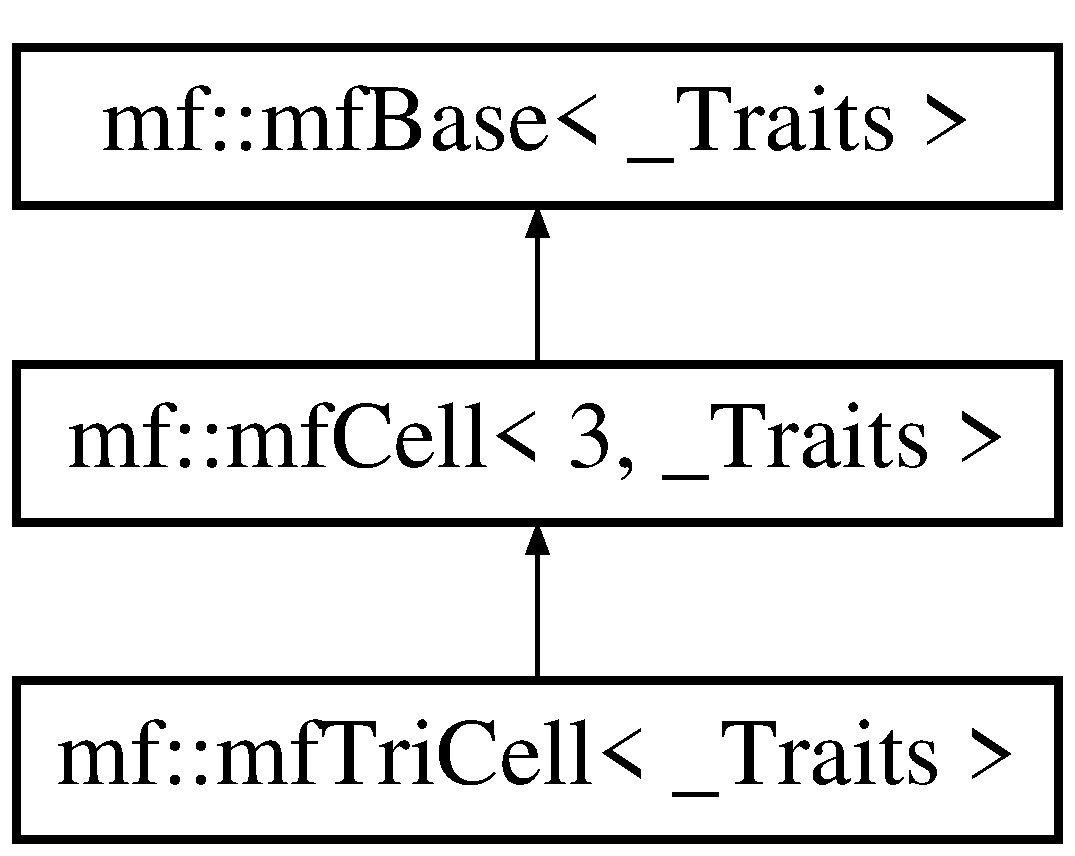
\includegraphics[height=3.000000cm]{classmf_1_1mfTriCell}
\end{center}
\end{figure}
\subsection*{Public Types}
\begin{DoxyCompactItemize}
\item 
typedef \_\-Traits::ids \hyperlink{classmf_1_1mfTriCell_ae8b5f3ec0b85289a7f8b39e1869458e4}{ids}
\end{DoxyCompactItemize}
\subsection*{Public Member Functions}
\begin{DoxyCompactItemize}
\item 
\hyperlink{classmf_1_1mfTriCell_a9a0ee46760e2e224af8d39ce62a0db9e}{mfTriCell} ()
\item 
virtual \hyperlink{classmf_1_1mfTriCell_aa409ed9b738e347231c2920e290c8b47}{$\sim$mfTriCell} ()
\item 
\hyperlink{classmf_1_1mfBase_a3b23f16ddf59da0a91ab12cf57c1f111}{ids} \hyperlink{classmf_1_1mfTriCell_af546fcd05bfbeba9291e91ea91d8706a}{getEdgeId} (int index MF\_\-DMUTEXVD)
\item 
void \hyperlink{classmf_1_1mfTriCell_a7603181ad8135d52001ee1e5f7108621}{setEdgeId} (int index, \hyperlink{classmf_1_1mfBase_a3b23f16ddf59da0a91ab12cf57c1f111}{ids} edge MF\_\-DMUTEXVD)
\end{DoxyCompactItemize}
\subsubsection*{template$<$class \_\-Traits$>$ class mf::mfTriCell$<$ \_\-Traits $>$}



\subsection{Member Typedef Documentation}
\hypertarget{classmf_1_1mfTriCell_ae8b5f3ec0b85289a7f8b39e1869458e4}{
\index{mf::mfTriCell@{mf::mfTriCell}!ids@{ids}}
\index{ids@{ids}!mf::mfTriCell@{mf::mfTriCell}}
\subsubsection[{ids}]{\setlength{\rightskip}{0pt plus 5cm}template$<$class \_\-Traits $>$ typedef \_\-Traits ::{\bf ids} {\bf mf::mfTriCell}$<$ \_\-Traits $>$::{\bf ids}}}
\label{classmf_1_1mfTriCell_ae8b5f3ec0b85289a7f8b39e1869458e4}
Id typename definition 

Reimplemented from \hyperlink{classmf_1_1mfCell_a9e32102899fb1e6b5e95b08a6c71063f}{mf::mfCell$<$ 3, \_\-Traits $>$}.



\subsection{Constructor \& Destructor Documentation}
\hypertarget{classmf_1_1mfTriCell_a9a0ee46760e2e224af8d39ce62a0db9e}{
\index{mf::mfTriCell@{mf::mfTriCell}!mfTriCell@{mfTriCell}}
\index{mfTriCell@{mfTriCell}!mf::mfTriCell@{mf::mfTriCell}}
\subsubsection[{mfTriCell}]{\setlength{\rightskip}{0pt plus 5cm}template$<$class \_\-Traits $>$ {\bf mf::mfTriCell}$<$ \_\-Traits $>$::{\bf mfTriCell} (
\begin{DoxyParamCaption}
{}
\end{DoxyParamCaption}
)}}
\label{classmf_1_1mfTriCell_a9a0ee46760e2e224af8d39ce62a0db9e}
Constructor \hypertarget{classmf_1_1mfTriCell_aa409ed9b738e347231c2920e290c8b47}{
\index{mf::mfTriCell@{mf::mfTriCell}!$\sim$mfTriCell@{$\sim$mfTriCell}}
\index{$\sim$mfTriCell@{$\sim$mfTriCell}!mf::mfTriCell@{mf::mfTriCell}}
\subsubsection[{$\sim$mfTriCell}]{\setlength{\rightskip}{0pt plus 5cm}template$<$class \_\-Traits $>$ {\bf mf::mfTriCell}$<$ \_\-Traits $>$::$\sim${\bf mfTriCell} (
\begin{DoxyParamCaption}
{}
\end{DoxyParamCaption}
)\hspace{0.3cm}{\ttfamily  \mbox{[}virtual\mbox{]}}}}
\label{classmf_1_1mfTriCell_aa409ed9b738e347231c2920e290c8b47}
Destructor 

\subsection{Member Function Documentation}
\hypertarget{classmf_1_1mfTriCell_af546fcd05bfbeba9291e91ea91d8706a}{
\index{mf::mfTriCell@{mf::mfTriCell}!getEdgeId@{getEdgeId}}
\index{getEdgeId@{getEdgeId}!mf::mfTriCell@{mf::mfTriCell}}
\subsubsection[{getEdgeId}]{\setlength{\rightskip}{0pt plus 5cm}template$<$class \_\-Traits $>$ IDS {\bf mf::mfTriCell}$<$ \_\-Traits $>$::getEdgeId (
\begin{DoxyParamCaption}
\item[{int index}]{MF\_\-DMUTEXVD}
\end{DoxyParamCaption}
)}}
\label{classmf_1_1mfTriCell_af546fcd05bfbeba9291e91ea91d8706a}
Return the edge id of the specified index


\begin{DoxyParams}{Parameters}
{\em index,:} & position of edge \\
\hline
\end{DoxyParams}
\hypertarget{classmf_1_1mfTriCell_a7603181ad8135d52001ee1e5f7108621}{
\index{mf::mfTriCell@{mf::mfTriCell}!setEdgeId@{setEdgeId}}
\index{setEdgeId@{setEdgeId}!mf::mfTriCell@{mf::mfTriCell}}
\subsubsection[{setEdgeId}]{\setlength{\rightskip}{0pt plus 5cm}template$<$class \_\-Traits $>$ void {\bf mf::mfTriCell}$<$ \_\-Traits $>$::setEdgeId (
\begin{DoxyParamCaption}
\item[{int}]{index, }
\item[{{\bf ids} edge}]{MF\_\-DMUTEXVD}
\end{DoxyParamCaption}
)}}
\label{classmf_1_1mfTriCell_a7603181ad8135d52001ee1e5f7108621}
Define the edge id of the specified index


\begin{DoxyParams}{Parameters}
{\em index,:} & position of edge \\
\hline
{\em vertex,:} & the edge id \\
\hline
\end{DoxyParams}


The documentation for this class was generated from the following file:\begin{DoxyCompactItemize}
\item 
\hyperlink{mfTriCell_8h}{mfTriCell.h}\end{DoxyCompactItemize}

\hypertarget{classmf_1_1mfVector}{
\section{mf::mfVector$<$ T, ids $>$ Class Template Reference}
\label{classmf_1_1mfVector}\index{mf::mfVector@{mf::mfVector}}
}
\subsection*{Public Member Functions}
\begin{DoxyCompactItemize}
\item 
\hyperlink{classmf_1_1mfVector_a0da8bd0ec9d950ea861483a98742279f}{mfVector} (ids block\_\-size)
\item 
\hyperlink{classmf_1_1mfVector_a0a4211f585fb4c90903f4fb4cb537ffc}{$\sim$mfVector} ()
\item 
T \& \hyperlink{classmf_1_1mfVector_a64e970f09bc93f29cfb1c13f5d4b94c3}{operator\mbox{[}$\,$\mbox{]}} (ids index)
\item 
ids \hyperlink{classmf_1_1mfVector_a85cba970ce38323288765a11bd0a321d}{getFree} ()
\item 
void \hyperlink{classmf_1_1mfVector_a998fc56f4b71456e2f9190a187137ac5}{setSize} (ids size)
\item 
ids \hyperlink{classmf_1_1mfVector_aa17e54b06d847676e2a04e039f4a794c}{getSize} ()
\item 
ids \hyperlink{classmf_1_1mfVector_a02d620a56b57de218bf625192a6b5134}{getMaxId} ()
\item 
bool \hyperlink{classmf_1_1mfVector_a344ecc1e67e566793948a5c0152944aa}{free} (ids index)
\end{DoxyCompactItemize}
\subsubsection*{template$<$class T, class ids$>$ class mf::mfVector$<$ T, ids $>$}



\subsection{Constructor \& Destructor Documentation}
\hypertarget{classmf_1_1mfVector_a0da8bd0ec9d950ea861483a98742279f}{
\index{mf::mfVector@{mf::mfVector}!mfVector@{mfVector}}
\index{mfVector@{mfVector}!mf::mfVector@{mf::mfVector}}
\subsubsection[{mfVector}]{\setlength{\rightskip}{0pt plus 5cm}template$<$class T , class ids$>$ {\bf mf::mfVector}$<$ T, ids $>$::{\bf mfVector} (
\begin{DoxyParamCaption}
\item[{ids}]{block\_\-size}
\end{DoxyParamCaption}
)}}
\label{classmf_1_1mfVector_a0da8bd0ec9d950ea861483a98742279f}
Constructor


\begin{DoxyParams}{Parameters}
{\em block\_\-size,:} & the size of each block (The maximum capacity of vector if : block\_\-size $\ast$ block\_\-size) \\
\hline
\end{DoxyParams}
\hypertarget{classmf_1_1mfVector_a0a4211f585fb4c90903f4fb4cb537ffc}{
\index{mf::mfVector@{mf::mfVector}!$\sim$mfVector@{$\sim$mfVector}}
\index{$\sim$mfVector@{$\sim$mfVector}!mf::mfVector@{mf::mfVector}}
\subsubsection[{$\sim$mfVector}]{\setlength{\rightskip}{0pt plus 5cm}template$<$class T , class ids $>$ {\bf mf::mfVector}$<$ T, ids $>$::$\sim${\bf mfVector} (
\begin{DoxyParamCaption}
{}
\end{DoxyParamCaption}
)}}
\label{classmf_1_1mfVector_a0a4211f585fb4c90903f4fb4cb537ffc}
Destructor 

\subsection{Member Function Documentation}
\hypertarget{classmf_1_1mfVector_a344ecc1e67e566793948a5c0152944aa}{
\index{mf::mfVector@{mf::mfVector}!free@{free}}
\index{free@{free}!mf::mfVector@{mf::mfVector}}
\subsubsection[{free}]{\setlength{\rightskip}{0pt plus 5cm}template$<$class T , class ids$>$ bool {\bf mf::mfVector}$<$ T, ids $>$::free (
\begin{DoxyParamCaption}
\item[{ids}]{index}
\end{DoxyParamCaption}
)}}
\label{classmf_1_1mfVector_a344ecc1e67e566793948a5c0152944aa}
Delete a position in vector

\begin{DoxyReturn}{Returns}
true if this position was deleted 
\end{DoxyReturn}
\hypertarget{classmf_1_1mfVector_a85cba970ce38323288765a11bd0a321d}{
\index{mf::mfVector@{mf::mfVector}!getFree@{getFree}}
\index{getFree@{getFree}!mf::mfVector@{mf::mfVector}}
\subsubsection[{getFree}]{\setlength{\rightskip}{0pt plus 5cm}template$<$class T , class ids $>$ ids {\bf mf::mfVector}$<$ T, ids $>$::getFree (
\begin{DoxyParamCaption}
{}
\end{DoxyParamCaption}
)}}
\label{classmf_1_1mfVector_a85cba970ce38323288765a11bd0a321d}
Return a free position in vector \hypertarget{classmf_1_1mfVector_a02d620a56b57de218bf625192a6b5134}{
\index{mf::mfVector@{mf::mfVector}!getMaxId@{getMaxId}}
\index{getMaxId@{getMaxId}!mf::mfVector@{mf::mfVector}}
\subsubsection[{getMaxId}]{\setlength{\rightskip}{0pt plus 5cm}template$<$class T , class ids $>$ ids {\bf mf::mfVector}$<$ T, ids $>$::getMaxId (
\begin{DoxyParamCaption}
{}
\end{DoxyParamCaption}
)}}
\label{classmf_1_1mfVector_a02d620a56b57de218bf625192a6b5134}
Return the maximum position in vector \hypertarget{classmf_1_1mfVector_aa17e54b06d847676e2a04e039f4a794c}{
\index{mf::mfVector@{mf::mfVector}!getSize@{getSize}}
\index{getSize@{getSize}!mf::mfVector@{mf::mfVector}}
\subsubsection[{getSize}]{\setlength{\rightskip}{0pt plus 5cm}template$<$class T , class ids $>$ ids {\bf mf::mfVector}$<$ T, ids $>$::getSize (
\begin{DoxyParamCaption}
{}
\end{DoxyParamCaption}
)}}
\label{classmf_1_1mfVector_aa17e54b06d847676e2a04e039f4a794c}
Return the number of elements in vector \hypertarget{classmf_1_1mfVector_a64e970f09bc93f29cfb1c13f5d4b94c3}{
\index{mf::mfVector@{mf::mfVector}!operator\mbox{[}\mbox{]}@{operator[]}}
\index{operator\mbox{[}\mbox{]}@{operator[]}!mf::mfVector@{mf::mfVector}}
\subsubsection[{operator[]}]{\setlength{\rightskip}{0pt plus 5cm}template$<$class T , class ids$>$ T \& {\bf mf::mfVector}$<$ T, ids $>$::operator\mbox{[}$\,$\mbox{]} (
\begin{DoxyParamCaption}
\item[{ids}]{index}
\end{DoxyParamCaption}
)}}
\label{classmf_1_1mfVector_a64e970f09bc93f29cfb1c13f5d4b94c3}
Return the specified element


\begin{DoxyParams}{Parameters}
{\em index,:} & position of element \\
\hline
\end{DoxyParams}
\hypertarget{classmf_1_1mfVector_a998fc56f4b71456e2f9190a187137ac5}{
\index{mf::mfVector@{mf::mfVector}!setSize@{setSize}}
\index{setSize@{setSize}!mf::mfVector@{mf::mfVector}}
\subsubsection[{setSize}]{\setlength{\rightskip}{0pt plus 5cm}template$<$class T , class ids$>$ void {\bf mf::mfVector}$<$ T, ids $>$::setSize (
\begin{DoxyParamCaption}
\item[{ids}]{size}
\end{DoxyParamCaption}
)}}
\label{classmf_1_1mfVector_a998fc56f4b71456e2f9190a187137ac5}
Define the number of elements in vector

(DONT USE) 

The documentation for this class was generated from the following file:\begin{DoxyCompactItemize}
\item 
\hyperlink{mfVector_8h}{mfVector.h}\end{DoxyCompactItemize}

\hypertarget{classmf_1_1mfVertex}{
\section{mf::mfVertex$<$ size, \_\-Traits $>$ Class Template Reference}
\label{classmf_1_1mfVertex}\index{mf::mfVertex@{mf::mfVertex}}
}
Inheritance diagram for mf::mfVertex$<$ size, \_\-Traits $>$:\begin{figure}[H]
\begin{center}
\leavevmode
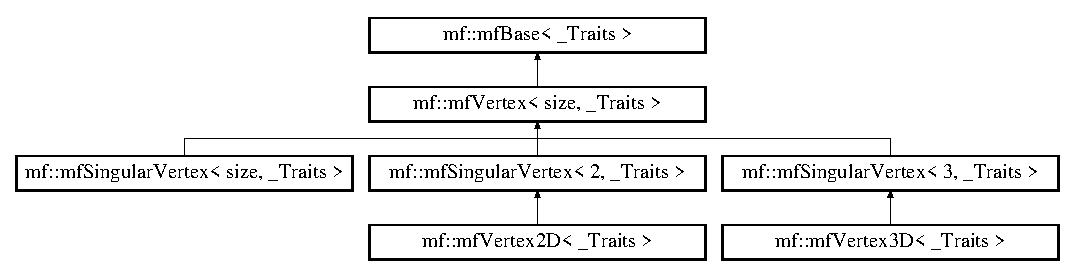
\includegraphics[height=3.260553cm]{classmf_1_1mfVertex}
\end{center}
\end{figure}
\subsection*{Public Types}
\begin{DoxyCompactItemize}
\item 
typedef \_\-Traits::space \hyperlink{classmf_1_1mfVertex_a9710b0b7ac7bbb276e1e97d541cbfc93}{space}
\end{DoxyCompactItemize}
\subsection*{Public Member Functions}
\begin{DoxyCompactItemize}
\item 
\hyperlink{classmf_1_1mfVertex_acfdae23d2d64be447df1e725eb37120f}{mfVertex} ()
\item 
virtual \hyperlink{classmf_1_1mfVertex_a82c8d82620afe828d321cd9c2fbb407b}{$\sim$mfVertex} ()
\item 
\hyperlink{classmf_1_1mfVertex_a9710b0b7ac7bbb276e1e97d541cbfc93}{space} \hyperlink{classmf_1_1mfVertex_aceb8aeb8d52129dd95a3b7948331754a}{getCoord} (int pos MF\_\-DMUTEXVD)
\item 
\hyperlink{classmf_1_1mfVertex_a9710b0b7ac7bbb276e1e97d541cbfc93}{space} $\ast$ \hyperlink{classmf_1_1mfVertex_a0dd251655f259788f1e921a97f425479}{getCoords} (MF\_\-DMUTEXD)
\item 
void \hyperlink{classmf_1_1mfVertex_ad4bb51f29cc783a6ec3a4b91ead078c1}{setCoord} (int pos, \hyperlink{classmf_1_1mfVertex_a9710b0b7ac7bbb276e1e97d541cbfc93}{space} value MF\_\-DMUTEXVD)
\item 
void \hyperlink{classmf_1_1mfVertex_a1fb5e4532e14904f853b1d261bb0f977}{setCoords} (\hyperlink{classmf_1_1mfVertex_a9710b0b7ac7bbb276e1e97d541cbfc93}{space} $\ast$values MF\_\-DMUTEXVD)
\end{DoxyCompactItemize}
\subsection*{Static Public Member Functions}
\begin{DoxyCompactItemize}
\item 
static int \hyperlink{classmf_1_1mfVertex_a6698049cfa3351294d3f96a3779af628}{getDimension} ()
\end{DoxyCompactItemize}
\subsubsection*{template$<$int size, class \_\-Traits$>$ class mf::mfVertex$<$ size, \_\-Traits $>$}



\subsection{Member Typedef Documentation}
\hypertarget{classmf_1_1mfVertex_a9710b0b7ac7bbb276e1e97d541cbfc93}{
\index{mf::mfVertex@{mf::mfVertex}!space@{space}}
\index{space@{space}!mf::mfVertex@{mf::mfVertex}}
\subsubsection[{space}]{\setlength{\rightskip}{0pt plus 5cm}template$<$int size, class \_\-Traits $>$ typedef \_\-Traits::space {\bf mf::mfVertex}$<$ size, \_\-Traits $>$::{\bf space}}}
\label{classmf_1_1mfVertex_a9710b0b7ac7bbb276e1e97d541cbfc93}
Space typename definition 

Reimplemented in \hyperlink{classmf_1_1mfSingularVertex_a96d4909dd62a8e8889eda76d0148db2a}{mf::mfSingularVertex$<$ size, \_\-Traits $>$}, \hyperlink{classmf_1_1mfVertex2D_a0730a219bea43b0b049cae2b4c72527b}{mf::mfVertex2D$<$ \_\-Traits $>$}, \hyperlink{classmf_1_1mfVertex3D_a16aa06a4ca21fae048fa56b7a40ac088}{mf::mfVertex3D$<$ \_\-Traits $>$}, \hyperlink{classmf_1_1mfSingularVertex_a96d4909dd62a8e8889eda76d0148db2a}{mf::mfSingularVertex$<$ 2, \_\-Traits $>$}, and \hyperlink{classmf_1_1mfSingularVertex_a96d4909dd62a8e8889eda76d0148db2a}{mf::mfSingularVertex$<$ 3, \_\-Traits $>$}.



\subsection{Constructor \& Destructor Documentation}
\hypertarget{classmf_1_1mfVertex_acfdae23d2d64be447df1e725eb37120f}{
\index{mf::mfVertex@{mf::mfVertex}!mfVertex@{mfVertex}}
\index{mfVertex@{mfVertex}!mf::mfVertex@{mf::mfVertex}}
\subsubsection[{mfVertex}]{\setlength{\rightskip}{0pt plus 5cm}template$<$int size, class \_\-Traits $>$ {\bf mf::mfVertex}$<$ size, \_\-Traits $>$::{\bf mfVertex} (
\begin{DoxyParamCaption}
{}
\end{DoxyParamCaption}
)}}
\label{classmf_1_1mfVertex_acfdae23d2d64be447df1e725eb37120f}
Constructor \hypertarget{classmf_1_1mfVertex_a82c8d82620afe828d321cd9c2fbb407b}{
\index{mf::mfVertex@{mf::mfVertex}!$\sim$mfVertex@{$\sim$mfVertex}}
\index{$\sim$mfVertex@{$\sim$mfVertex}!mf::mfVertex@{mf::mfVertex}}
\subsubsection[{$\sim$mfVertex}]{\setlength{\rightskip}{0pt plus 5cm}template$<$int size, class \_\-Traits $>$ {\bf mf::mfVertex}$<$ size, \_\-Traits $>$::$\sim${\bf mfVertex} (
\begin{DoxyParamCaption}
{}
\end{DoxyParamCaption}
)\hspace{0.3cm}{\ttfamily  \mbox{[}virtual\mbox{]}}}}
\label{classmf_1_1mfVertex_a82c8d82620afe828d321cd9c2fbb407b}
Destructor 

\subsection{Member Function Documentation}
\hypertarget{classmf_1_1mfVertex_aceb8aeb8d52129dd95a3b7948331754a}{
\index{mf::mfVertex@{mf::mfVertex}!getCoord@{getCoord}}
\index{getCoord@{getCoord}!mf::mfVertex@{mf::mfVertex}}
\subsubsection[{getCoord}]{\setlength{\rightskip}{0pt plus 5cm}template$<$int size, class \_\-Traits $>$ SPACE {\bf mf::mfVertex}$<$ size, \_\-Traits $>$::getCoord (
\begin{DoxyParamCaption}
\item[{int pos}]{MF\_\-DMUTEXVD}
\end{DoxyParamCaption}
)}}
\label{classmf_1_1mfVertex_aceb8aeb8d52129dd95a3b7948331754a}
Return a specified coordinate of a vertex


\begin{DoxyParams}{Parameters}
{\em pos,:} & index of coordinate (1=x, 2=y, 3=z) \\
\hline
\end{DoxyParams}
\begin{DoxyReturn}{Returns}
Value of the coordinate indexed by pos. 
\end{DoxyReturn}
\hypertarget{classmf_1_1mfVertex_a0dd251655f259788f1e921a97f425479}{
\index{mf::mfVertex@{mf::mfVertex}!getCoords@{getCoords}}
\index{getCoords@{getCoords}!mf::mfVertex@{mf::mfVertex}}
\subsubsection[{getCoords}]{\setlength{\rightskip}{0pt plus 5cm}template$<$int size, class \_\-Traits $>$ SPACE $\ast$ {\bf mf::mfVertex}$<$ size, \_\-Traits $>$::getCoords (
\begin{DoxyParamCaption}
\item[{MF\_\-DMUTEXD}]{}
\end{DoxyParamCaption}
)}}
\label{classmf_1_1mfVertex_a0dd251655f259788f1e921a97f425479}
Return a vector of all coordinates

\begin{DoxyReturn}{Returns}
Vector with coordinates values of the vertex. 
\end{DoxyReturn}
\hypertarget{classmf_1_1mfVertex_a6698049cfa3351294d3f96a3779af628}{
\index{mf::mfVertex@{mf::mfVertex}!getDimension@{getDimension}}
\index{getDimension@{getDimension}!mf::mfVertex@{mf::mfVertex}}
\subsubsection[{getDimension}]{\setlength{\rightskip}{0pt plus 5cm}template$<$int size, class \_\-Traits $>$ static int {\bf mf::mfVertex}$<$ size, \_\-Traits $>$::getDimension (
\begin{DoxyParamCaption}
{}
\end{DoxyParamCaption}
)\hspace{0.3cm}{\ttfamily  \mbox{[}inline, static\mbox{]}}}}
\label{classmf_1_1mfVertex_a6698049cfa3351294d3f96a3779af628}
Return the dimension of the vertex

\begin{DoxyReturn}{Returns}
Dimension of the vertex (2D or 3D). 
\end{DoxyReturn}
\hypertarget{classmf_1_1mfVertex_ad4bb51f29cc783a6ec3a4b91ead078c1}{
\index{mf::mfVertex@{mf::mfVertex}!setCoord@{setCoord}}
\index{setCoord@{setCoord}!mf::mfVertex@{mf::mfVertex}}
\subsubsection[{setCoord}]{\setlength{\rightskip}{0pt plus 5cm}template$<$int size, class \_\-Traits $>$ void {\bf mf::mfVertex}$<$ size, \_\-Traits $>$::setCoord (
\begin{DoxyParamCaption}
\item[{int}]{pos, }
\item[{{\bf space} value}]{MF\_\-DMUTEXVD}
\end{DoxyParamCaption}
)}}
\label{classmf_1_1mfVertex_ad4bb51f29cc783a6ec3a4b91ead078c1}
Define the specified coordinate value


\begin{DoxyParams}{Parameters}
{\em pos,:} & index of coordinate (1=x, 2=y, 3=z) \\
\hline
{\em value,:} & coordinate value \\
\hline
\end{DoxyParams}
\hypertarget{classmf_1_1mfVertex_a1fb5e4532e14904f853b1d261bb0f977}{
\index{mf::mfVertex@{mf::mfVertex}!setCoords@{setCoords}}
\index{setCoords@{setCoords}!mf::mfVertex@{mf::mfVertex}}
\subsubsection[{setCoords}]{\setlength{\rightskip}{0pt plus 5cm}template$<$int size, class \_\-Traits $>$ void {\bf mf::mfVertex}$<$ size, \_\-Traits $>$::setCoords (
\begin{DoxyParamCaption}
\item[{{\bf space} $\ast$values}]{MF\_\-DMUTEXVD}
\end{DoxyParamCaption}
)}}
\label{classmf_1_1mfVertex_a1fb5e4532e14904f853b1d261bb0f977}
Define all coordinates values


\begin{DoxyParams}{Parameters}
{\em values,:} & vector with coordinates values \\
\hline
\end{DoxyParams}


The documentation for this class was generated from the following file:\begin{DoxyCompactItemize}
\item 
\hyperlink{mfVertex_8h}{mfVertex.h}\end{DoxyCompactItemize}

\hypertarget{classmf_1_1mfVertex2D}{
\section{mf::mfVertex2D$<$ \_\-Traits $>$ Class Template Reference}
\label{classmf_1_1mfVertex2D}\index{mf::mfVertex2D@{mf::mfVertex2D}}
}
Inheritance diagram for mf::mfVertex2D$<$ \_\-Traits $>$:\begin{figure}[H]
\begin{center}
\leavevmode
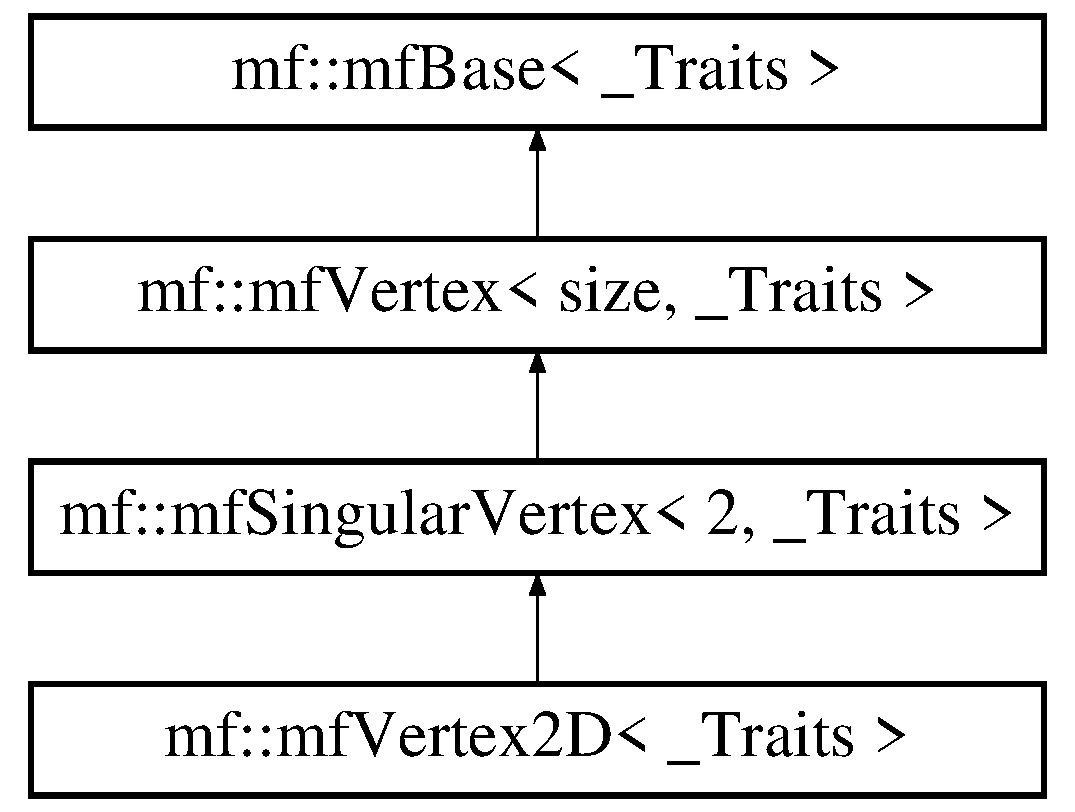
\includegraphics[height=4.000000cm]{classmf_1_1mfVertex2D}
\end{center}
\end{figure}
\subsection*{Public Types}
\begin{DoxyCompactItemize}
\item 
typedef \_\-Traits::space \hyperlink{classmf_1_1mfVertex2D_a0730a219bea43b0b049cae2b4c72527b}{space}
\end{DoxyCompactItemize}
\subsection*{Public Member Functions}
\begin{DoxyCompactItemize}
\item 
\hyperlink{classmf_1_1mfVertex2D_a0e8d7770cc851b6e5ebfad22730c7e9c}{mfVertex2D} ()
\item 
\hyperlink{classmf_1_1mfVertex2D_ac81496cd8d9193bab0e9cde62fa891e4}{mfVertex2D} (\hyperlink{classmf_1_1mfVertex_a9710b0b7ac7bbb276e1e97d541cbfc93}{space} x, \hyperlink{classmf_1_1mfVertex_a9710b0b7ac7bbb276e1e97d541cbfc93}{space} y)
\item 
\hyperlink{classmf_1_1mfVertex2D_a9f275e28ff046869c8ce6345fe2d9f15}{$\sim$mfVertex2D} ()
\end{DoxyCompactItemize}
\subsubsection*{template$<$class \_\-Traits$>$ class mf::mfVertex2D$<$ \_\-Traits $>$}



\subsection{Member Typedef Documentation}
\hypertarget{classmf_1_1mfVertex2D_a0730a219bea43b0b049cae2b4c72527b}{
\index{mf::mfVertex2D@{mf::mfVertex2D}!space@{space}}
\index{space@{space}!mf::mfVertex2D@{mf::mfVertex2D}}
\subsubsection[{space}]{\setlength{\rightskip}{0pt plus 5cm}template$<$class \_\-Traits $>$ typedef \_\-Traits::space {\bf mf::mfVertex2D}$<$ \_\-Traits $>$::{\bf space}}}
\label{classmf_1_1mfVertex2D_a0730a219bea43b0b049cae2b4c72527b}
Space typename definition 

Reimplemented from \hyperlink{classmf_1_1mfSingularVertex_a96d4909dd62a8e8889eda76d0148db2a}{mf::mfSingularVertex$<$ 2, \_\-Traits $>$}.



\subsection{Constructor \& Destructor Documentation}
\hypertarget{classmf_1_1mfVertex2D_a0e8d7770cc851b6e5ebfad22730c7e9c}{
\index{mf::mfVertex2D@{mf::mfVertex2D}!mfVertex2D@{mfVertex2D}}
\index{mfVertex2D@{mfVertex2D}!mf::mfVertex2D@{mf::mfVertex2D}}
\subsubsection[{mfVertex2D}]{\setlength{\rightskip}{0pt plus 5cm}template$<$class \_\-Traits $>$ {\bf mf::mfVertex2D}$<$ \_\-Traits $>$::{\bf mfVertex2D} (
\begin{DoxyParamCaption}
{}
\end{DoxyParamCaption}
)}}
\label{classmf_1_1mfVertex2D_a0e8d7770cc851b6e5ebfad22730c7e9c}
Constructor \hypertarget{classmf_1_1mfVertex2D_ac81496cd8d9193bab0e9cde62fa891e4}{
\index{mf::mfVertex2D@{mf::mfVertex2D}!mfVertex2D@{mfVertex2D}}
\index{mfVertex2D@{mfVertex2D}!mf::mfVertex2D@{mf::mfVertex2D}}
\subsubsection[{mfVertex2D}]{\setlength{\rightskip}{0pt plus 5cm}template$<$class \_\-Traits $>$ {\bf mf::mfVertex2D}$<$ \_\-Traits $>$::{\bf mfVertex2D} (
\begin{DoxyParamCaption}
\item[{{\bf space}}]{x, }
\item[{{\bf space}}]{y}
\end{DoxyParamCaption}
)}}
\label{classmf_1_1mfVertex2D_ac81496cd8d9193bab0e9cde62fa891e4}
Constructor


\begin{DoxyParams}{Parameters}
{\em x,:} & x coordinate value to be initialized \\
\hline
{\em y,:} & y coordinate value to be initialized \\
\hline
\end{DoxyParams}
\hypertarget{classmf_1_1mfVertex2D_a9f275e28ff046869c8ce6345fe2d9f15}{
\index{mf::mfVertex2D@{mf::mfVertex2D}!$\sim$mfVertex2D@{$\sim$mfVertex2D}}
\index{$\sim$mfVertex2D@{$\sim$mfVertex2D}!mf::mfVertex2D@{mf::mfVertex2D}}
\subsubsection[{$\sim$mfVertex2D}]{\setlength{\rightskip}{0pt plus 5cm}template$<$class \_\-Traits $>$ {\bf mf::mfVertex2D}$<$ \_\-Traits $>$::$\sim${\bf mfVertex2D} (
\begin{DoxyParamCaption}
{}
\end{DoxyParamCaption}
)}}
\label{classmf_1_1mfVertex2D_a9f275e28ff046869c8ce6345fe2d9f15}
Destructor 

The documentation for this class was generated from the following file:\begin{DoxyCompactItemize}
\item 
\hyperlink{mfVertex2D_8h}{mfVertex2D.h}\end{DoxyCompactItemize}

\hypertarget{classmf_1_1mfVertex3D}{
\section{mf::mfVertex3D$<$ \_\-Traits $>$ Class Template Reference}
\label{classmf_1_1mfVertex3D}\index{mf::mfVertex3D@{mf::mfVertex3D}}
}
Inheritance diagram for mf::mfVertex3D$<$ \_\-Traits $>$:\begin{figure}[H]
\begin{center}
\leavevmode
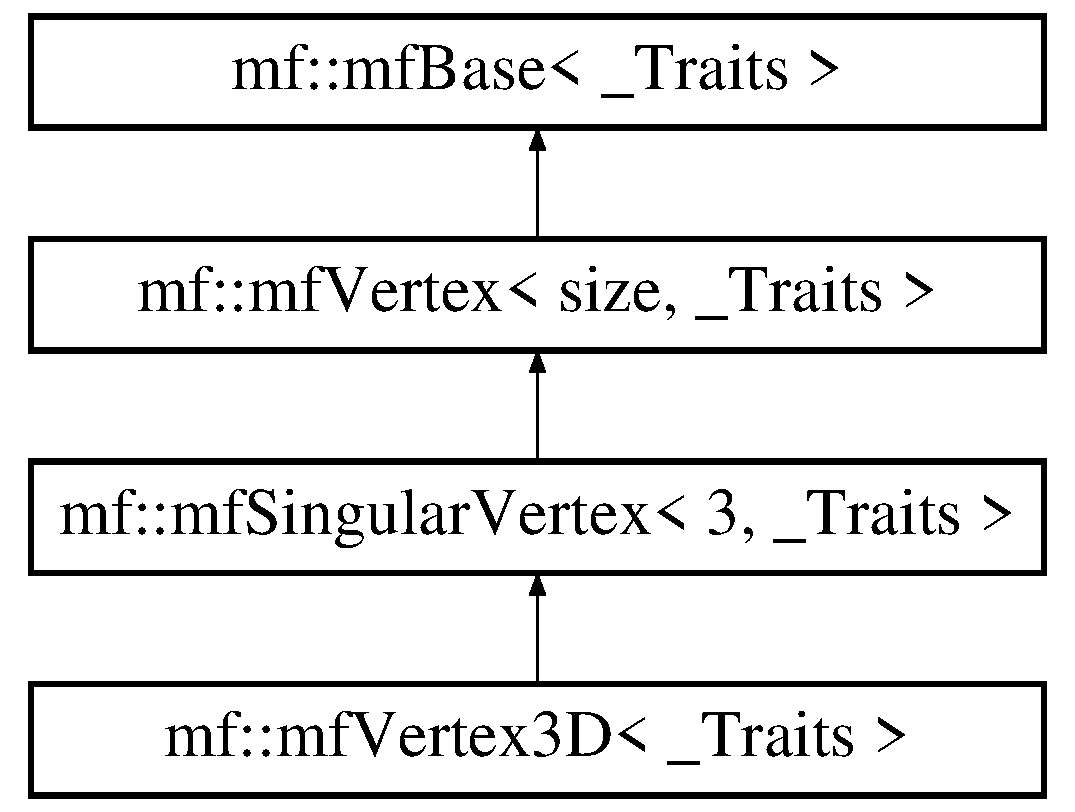
\includegraphics[height=4.000000cm]{classmf_1_1mfVertex3D}
\end{center}
\end{figure}
\subsection*{Public Types}
\begin{DoxyCompactItemize}
\item 
typedef \_\-Traits::space \hyperlink{classmf_1_1mfVertex3D_a16aa06a4ca21fae048fa56b7a40ac088}{space}
\end{DoxyCompactItemize}
\subsection*{Public Member Functions}
\begin{DoxyCompactItemize}
\item 
\hyperlink{classmf_1_1mfVertex3D_abbd39a1efcb4f29274f6457f9ee4126e}{mfVertex3D} ()
\item 
\hyperlink{classmf_1_1mfVertex3D_a6b9e354109039d64dacf2affbfb7a52d}{mfVertex3D} (\hyperlink{classmf_1_1mfVertex_a9710b0b7ac7bbb276e1e97d541cbfc93}{space} x, \hyperlink{classmf_1_1mfVertex_a9710b0b7ac7bbb276e1e97d541cbfc93}{space} y, \hyperlink{classmf_1_1mfVertex_a9710b0b7ac7bbb276e1e97d541cbfc93}{space} z)
\item 
\hyperlink{classmf_1_1mfVertex3D_aef3a46fb4c8ce5c1ec03e26c7e1b8901}{$\sim$mfVertex3D} ()
\end{DoxyCompactItemize}
\subsubsection*{template$<$class \_\-Traits$>$ class mf::mfVertex3D$<$ \_\-Traits $>$}



\subsection{Member Typedef Documentation}
\hypertarget{classmf_1_1mfVertex3D_a16aa06a4ca21fae048fa56b7a40ac088}{
\index{mf::mfVertex3D@{mf::mfVertex3D}!space@{space}}
\index{space@{space}!mf::mfVertex3D@{mf::mfVertex3D}}
\subsubsection[{space}]{\setlength{\rightskip}{0pt plus 5cm}template$<$class \_\-Traits $>$ typedef \_\-Traits::space {\bf mf::mfVertex3D}$<$ \_\-Traits $>$::{\bf space}}}
\label{classmf_1_1mfVertex3D_a16aa06a4ca21fae048fa56b7a40ac088}
Space typename definition 

Reimplemented from \hyperlink{classmf_1_1mfSingularVertex_a96d4909dd62a8e8889eda76d0148db2a}{mf::mfSingularVertex$<$ 3, \_\-Traits $>$}.



\subsection{Constructor \& Destructor Documentation}
\hypertarget{classmf_1_1mfVertex3D_abbd39a1efcb4f29274f6457f9ee4126e}{
\index{mf::mfVertex3D@{mf::mfVertex3D}!mfVertex3D@{mfVertex3D}}
\index{mfVertex3D@{mfVertex3D}!mf::mfVertex3D@{mf::mfVertex3D}}
\subsubsection[{mfVertex3D}]{\setlength{\rightskip}{0pt plus 5cm}template$<$class \_\-Traits $>$ {\bf mf::mfVertex3D}$<$ \_\-Traits $>$::{\bf mfVertex3D} (
\begin{DoxyParamCaption}
{}
\end{DoxyParamCaption}
)}}
\label{classmf_1_1mfVertex3D_abbd39a1efcb4f29274f6457f9ee4126e}
Constructor \hypertarget{classmf_1_1mfVertex3D_a6b9e354109039d64dacf2affbfb7a52d}{
\index{mf::mfVertex3D@{mf::mfVertex3D}!mfVertex3D@{mfVertex3D}}
\index{mfVertex3D@{mfVertex3D}!mf::mfVertex3D@{mf::mfVertex3D}}
\subsubsection[{mfVertex3D}]{\setlength{\rightskip}{0pt plus 5cm}template$<$class \_\-Traits $>$ {\bf mf::mfVertex3D}$<$ \_\-Traits $>$::{\bf mfVertex3D} (
\begin{DoxyParamCaption}
\item[{{\bf space}}]{x, }
\item[{{\bf space}}]{y, }
\item[{{\bf space}}]{z}
\end{DoxyParamCaption}
)}}
\label{classmf_1_1mfVertex3D_a6b9e354109039d64dacf2affbfb7a52d}
Constructor


\begin{DoxyParams}{Parameters}
{\em x,:} & x coordinate value to be initialized \\
\hline
{\em y,:} & y coordinate value to be initialized \\
\hline
{\em z,:} & z coordinate value to be initialized \\
\hline
\end{DoxyParams}
\hypertarget{classmf_1_1mfVertex3D_aef3a46fb4c8ce5c1ec03e26c7e1b8901}{
\index{mf::mfVertex3D@{mf::mfVertex3D}!$\sim$mfVertex3D@{$\sim$mfVertex3D}}
\index{$\sim$mfVertex3D@{$\sim$mfVertex3D}!mf::mfVertex3D@{mf::mfVertex3D}}
\subsubsection[{$\sim$mfVertex3D}]{\setlength{\rightskip}{0pt plus 5cm}template$<$class \_\-Traits $>$ {\bf mf::mfVertex3D}$<$ \_\-Traits $>$::$\sim${\bf mfVertex3D} (
\begin{DoxyParamCaption}
{}
\end{DoxyParamCaption}
)}}
\label{classmf_1_1mfVertex3D_aef3a46fb4c8ce5c1ec03e26c7e1b8901}
Destructor 

The documentation for this class was generated from the following file:\begin{DoxyCompactItemize}
\item 
mfVertex3D.h\end{DoxyCompactItemize}

\hypertarget{classmf_1_1mfVertexStarIterator2D}{
\section{mf::mfVertexStarIterator2D$<$ \_\-Traits $>$ Class Template Reference}
\label{classmf_1_1mfVertexStarIterator2D}\index{mf::mfVertexStarIterator2D@{mf::mfVertexStarIterator2D}}
}
Inheritance diagram for mf::mfVertexStarIterator2D$<$ \_\-Traits $>$:\begin{figure}[H]
\begin{center}
\leavevmode
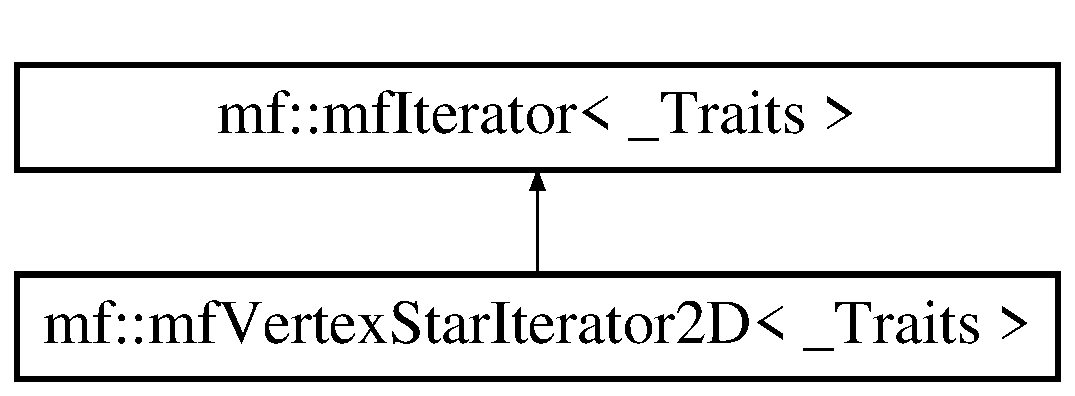
\includegraphics[height=2.000000cm]{classmf_1_1mfVertexStarIterator2D}
\end{center}
\end{figure}
\subsection*{Public Types}
\begin{DoxyCompactItemize}
\item 
\hypertarget{classmf_1_1mfVertexStarIterator2D_a96630336587c42a2d07492893180a46b}{
typedef \_\-Traits::sCell {\bfseries sCell}}
\label{classmf_1_1mfVertexStarIterator2D_a96630336587c42a2d07492893180a46b}

\item 
\hypertarget{classmf_1_1mfVertexStarIterator2D_a4d0bb9728998b79e239956f3deb70708}{
typedef \_\-Traits::sVertex {\bfseries sVertex}}
\label{classmf_1_1mfVertexStarIterator2D_a4d0bb9728998b79e239956f3deb70708}

\item 
\hypertarget{classmf_1_1mfVertexStarIterator2D_a4ea6ceb160b2e1817e4a98c0bf434819}{
typedef \_\-Traits::ids {\bfseries ids}}
\label{classmf_1_1mfVertexStarIterator2D_a4ea6ceb160b2e1817e4a98c0bf434819}

\item 
\hypertarget{classmf_1_1mfVertexStarIterator2D_a778a191ed8efe2e818a01caa69079817}{
typedef \hyperlink{classmf_1_1mfSing}{mfSing}$<$ \_\-Traits $>$ {\bfseries sSing}}
\label{classmf_1_1mfVertexStarIterator2D_a778a191ed8efe2e818a01caa69079817}

\item 
typedef \_\-Traits::sMesh \hyperlink{classmf_1_1mfVertexStarIterator2D_a25f97b24c35482b8677e4672d70687cf}{sMesh}
\end{DoxyCompactItemize}
\subsection*{Public Member Functions}
\begin{DoxyCompactItemize}
\item 
\hyperlink{classmf_1_1mfVertexStarIterator2D_ad0b86bd236b0a5e3bcd594c6f79e94c7}{mfVertexStarIterator2D} (\hyperlink{classmf_1_1mfIterator_aca31e4d7e7eca4e3b100530d8725064b}{sMesh} $\ast$\_\-mesh)
\item 
\hyperlink{classmf_1_1mfVertexStarIterator2D_a28c7d3235fd232a8881456a61bae6d02}{$\sim$mfVertexStarIterator2D} ()
\item 
\hypertarget{classmf_1_1mfVertexStarIterator2D_a4ad30c406b8449b415a1da3467438282}{
bool {\bfseries initialize} (ids init)}
\label{classmf_1_1mfVertexStarIterator2D_a4ad30c406b8449b415a1da3467438282}

\item 
\hypertarget{classmf_1_1mfVertexStarIterator2D_a38b904e0dcfcbdd0c349081f43621662}{
bool {\bfseries finish} ()}
\label{classmf_1_1mfVertexStarIterator2D_a38b904e0dcfcbdd0c349081f43621662}

\item 
\hypertarget{classmf_1_1mfVertexStarIterator2D_a387dd1cf9db316f8ef0034fc5e1a4c30}{
bool {\bfseries notFinish} ()}
\label{classmf_1_1mfVertexStarIterator2D_a387dd1cf9db316f8ef0034fc5e1a4c30}

\item 
\hypertarget{classmf_1_1mfVertexStarIterator2D_acaf33605c88155d3d843f454be9d7f2a}{
bool {\bfseries operator++} ()}
\label{classmf_1_1mfVertexStarIterator2D_acaf33605c88155d3d843f454be9d7f2a}

\item 
\hypertarget{classmf_1_1mfVertexStarIterator2D_aad1297b5024d1236666660419c8699d2}{
sCell $\ast$ {\bfseries operator-\/$>$} ()}
\label{classmf_1_1mfVertexStarIterator2D_aad1297b5024d1236666660419c8699d2}

\item 
\hypertarget{classmf_1_1mfVertexStarIterator2D_ab50b8139db709fd79e5aeb5f05253fc7}{
sCell $\ast$ {\bfseries operator$\ast$} ()}
\label{classmf_1_1mfVertexStarIterator2D_ab50b8139db709fd79e5aeb5f05253fc7}

\item 
\hypertarget{classmf_1_1mfVertexStarIterator2D_ab69d8b4494074c89685296fece780690}{
ids {\bfseries operator\&} ()}
\label{classmf_1_1mfVertexStarIterator2D_ab69d8b4494074c89685296fece780690}

\end{DoxyCompactItemize}
\subsubsection*{template$<$class \_\-Traits$>$ class mf::mfVertexStarIterator2D$<$ \_\-Traits $>$}



\subsection{Member Typedef Documentation}
\hypertarget{classmf_1_1mfVertexStarIterator2D_a25f97b24c35482b8677e4672d70687cf}{
\index{mf::mfVertexStarIterator2D@{mf::mfVertexStarIterator2D}!sMesh@{sMesh}}
\index{sMesh@{sMesh}!mf::mfVertexStarIterator2D@{mf::mfVertexStarIterator2D}}
\subsubsection[{sMesh}]{\setlength{\rightskip}{0pt plus 5cm}template$<$class \_\-Traits $>$ typedef \_\-Traits::sMesh {\bf mf::mfVertexStarIterator2D}$<$ \_\-Traits $>$::{\bf sMesh}}}
\label{classmf_1_1mfVertexStarIterator2D_a25f97b24c35482b8677e4672d70687cf}
Mesh typename definition 

Reimplemented from \hyperlink{classmf_1_1mfIterator_aca31e4d7e7eca4e3b100530d8725064b}{mf::mfIterator$<$ \_\-Traits $>$}.



\subsection{Constructor \& Destructor Documentation}
\hypertarget{classmf_1_1mfVertexStarIterator2D_ad0b86bd236b0a5e3bcd594c6f79e94c7}{
\index{mf::mfVertexStarIterator2D@{mf::mfVertexStarIterator2D}!mfVertexStarIterator2D@{mfVertexStarIterator2D}}
\index{mfVertexStarIterator2D@{mfVertexStarIterator2D}!mf::mfVertexStarIterator2D@{mf::mfVertexStarIterator2D}}
\subsubsection[{mfVertexStarIterator2D}]{\setlength{\rightskip}{0pt plus 5cm}template$<$class \_\-Traits $>$ {\bf mf::mfVertexStarIterator2D}$<$ \_\-Traits $>$::{\bf mfVertexStarIterator2D} (
\begin{DoxyParamCaption}
\item[{{\bf sMesh} $\ast$}]{\_\-mesh}
\end{DoxyParamCaption}
)}}
\label{classmf_1_1mfVertexStarIterator2D_ad0b86bd236b0a5e3bcd594c6f79e94c7}
Construtor \hypertarget{classmf_1_1mfVertexStarIterator2D_a28c7d3235fd232a8881456a61bae6d02}{
\index{mf::mfVertexStarIterator2D@{mf::mfVertexStarIterator2D}!$\sim$mfVertexStarIterator2D@{$\sim$mfVertexStarIterator2D}}
\index{$\sim$mfVertexStarIterator2D@{$\sim$mfVertexStarIterator2D}!mf::mfVertexStarIterator2D@{mf::mfVertexStarIterator2D}}
\subsubsection[{$\sim$mfVertexStarIterator2D}]{\setlength{\rightskip}{0pt plus 5cm}template$<$class \_\-Traits $>$ {\bf mf::mfVertexStarIterator2D}$<$ \_\-Traits $>$::$\sim${\bf mfVertexStarIterator2D} (
\begin{DoxyParamCaption}
{}
\end{DoxyParamCaption}
)}}
\label{classmf_1_1mfVertexStarIterator2D_a28c7d3235fd232a8881456a61bae6d02}
Destrutor 

The documentation for this class was generated from the following file:\begin{DoxyCompactItemize}
\item 
mfVertexStarIterator2D.h\end{DoxyCompactItemize}

\hypertarget{classmf_1_1mfVertexStarIterator3D}{
\section{mf::mfVertexStarIterator3D$<$ \_\-Traits $>$ Class Template Reference}
\label{classmf_1_1mfVertexStarIterator3D}\index{mf::mfVertexStarIterator3D@{mf::mfVertexStarIterator3D}}
}
Inheritance diagram for mf::mfVertexStarIterator3D$<$ \_\-Traits $>$:\begin{figure}[H]
\begin{center}
\leavevmode
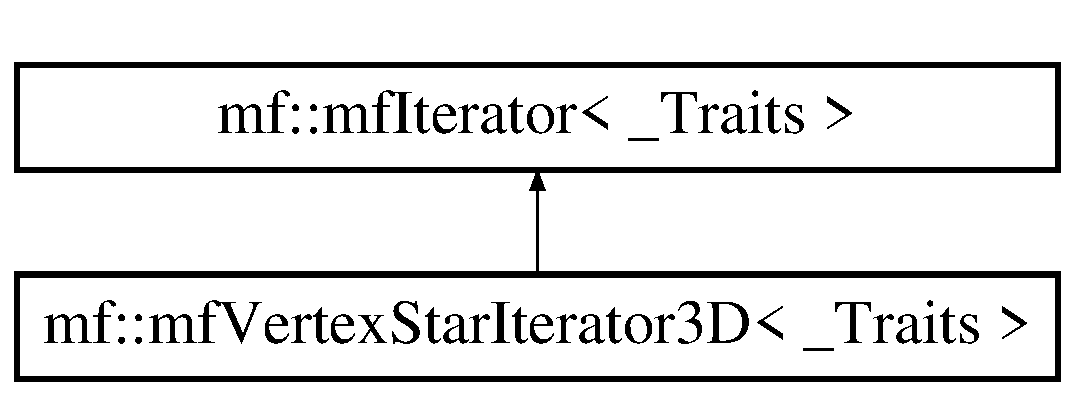
\includegraphics[height=2.000000cm]{classmf_1_1mfVertexStarIterator3D}
\end{center}
\end{figure}
\subsection*{Public Types}
\begin{DoxyCompactItemize}
\item 
\hypertarget{classmf_1_1mfVertexStarIterator3D_a55e757163cbd49e46e75a76033e694d0}{
typedef \_\-Traits::sCell {\bfseries sCell}}
\label{classmf_1_1mfVertexStarIterator3D_a55e757163cbd49e46e75a76033e694d0}

\item 
\hypertarget{classmf_1_1mfVertexStarIterator3D_aae63a088dc8b454ecc35ab4be6e41ccd}{
typedef \_\-Traits::sVertex {\bfseries sVertex}}
\label{classmf_1_1mfVertexStarIterator3D_aae63a088dc8b454ecc35ab4be6e41ccd}

\item 
\hypertarget{classmf_1_1mfVertexStarIterator3D_a663016294ac1e5461047aab8f87ce621}{
typedef \_\-Traits::ids {\bfseries ids}}
\label{classmf_1_1mfVertexStarIterator3D_a663016294ac1e5461047aab8f87ce621}

\item 
\hypertarget{classmf_1_1mfVertexStarIterator3D_a77654608fb1896295c324f7ac213d7ef}{
typedef \hyperlink{classmf_1_1mfSing}{mfSing}$<$ \_\-Traits $>$ {\bfseries sSing}}
\label{classmf_1_1mfVertexStarIterator3D_a77654608fb1896295c324f7ac213d7ef}

\item 
typedef \_\-Traits::sMesh \hyperlink{classmf_1_1mfVertexStarIterator3D_aa45e0318e1153d3b373ec69af44d6710}{sMesh}
\end{DoxyCompactItemize}
\subsection*{Public Member Functions}
\begin{DoxyCompactItemize}
\item 
\hyperlink{classmf_1_1mfVertexStarIterator3D_a0602e37cf9ad3c3ec4d72684c2594c77}{mfVertexStarIterator3D} (\hyperlink{classmf_1_1mfIterator_aca31e4d7e7eca4e3b100530d8725064b}{sMesh} $\ast$\_\-mesh)
\item 
\hyperlink{classmf_1_1mfVertexStarIterator3D_a6fc44da5b33a391c7abd7e29dcd37d5c}{$\sim$mfVertexStarIterator3D} ()
\item 
\hypertarget{classmf_1_1mfVertexStarIterator3D_ad1bb694599a8648098b8d3e4e48f788c}{
bool {\bfseries initialize} (ids init)}
\label{classmf_1_1mfVertexStarIterator3D_ad1bb694599a8648098b8d3e4e48f788c}

\item 
\hypertarget{classmf_1_1mfVertexStarIterator3D_ad624324340f0d703ad758605bd4e8a78}{
bool {\bfseries finish} ()}
\label{classmf_1_1mfVertexStarIterator3D_ad624324340f0d703ad758605bd4e8a78}

\item 
\hypertarget{classmf_1_1mfVertexStarIterator3D_a929ffee847a4f36301154b8c741e9378}{
bool {\bfseries notFinish} ()}
\label{classmf_1_1mfVertexStarIterator3D_a929ffee847a4f36301154b8c741e9378}

\item 
\hypertarget{classmf_1_1mfVertexStarIterator3D_aa9757da8b9281d43f90f7d0643f3bf86}{
bool {\bfseries operator++} ()}
\label{classmf_1_1mfVertexStarIterator3D_aa9757da8b9281d43f90f7d0643f3bf86}

\item 
\hypertarget{classmf_1_1mfVertexStarIterator3D_afe865fa2a605861aa925c7aba56281a2}{
sCell $\ast$ {\bfseries operator-\/$>$} ()}
\label{classmf_1_1mfVertexStarIterator3D_afe865fa2a605861aa925c7aba56281a2}

\item 
\hypertarget{classmf_1_1mfVertexStarIterator3D_ae940b9144e4d09c80fba7778145a2bf2}{
sCell $\ast$ {\bfseries operator$\ast$} ()}
\label{classmf_1_1mfVertexStarIterator3D_ae940b9144e4d09c80fba7778145a2bf2}

\item 
\hypertarget{classmf_1_1mfVertexStarIterator3D_a9efd39ba01d0d9544b97ec97ad7b4a69}{
ids {\bfseries operator\&} ()}
\label{classmf_1_1mfVertexStarIterator3D_a9efd39ba01d0d9544b97ec97ad7b4a69}

\end{DoxyCompactItemize}
\subsubsection*{template$<$class \_\-Traits$>$ class mf::mfVertexStarIterator3D$<$ \_\-Traits $>$}



\subsection{Member Typedef Documentation}
\hypertarget{classmf_1_1mfVertexStarIterator3D_aa45e0318e1153d3b373ec69af44d6710}{
\index{mf::mfVertexStarIterator3D@{mf::mfVertexStarIterator3D}!sMesh@{sMesh}}
\index{sMesh@{sMesh}!mf::mfVertexStarIterator3D@{mf::mfVertexStarIterator3D}}
\subsubsection[{sMesh}]{\setlength{\rightskip}{0pt plus 5cm}template$<$class \_\-Traits $>$ typedef \_\-Traits::sMesh {\bf mf::mfVertexStarIterator3D}$<$ \_\-Traits $>$::{\bf sMesh}}}
\label{classmf_1_1mfVertexStarIterator3D_aa45e0318e1153d3b373ec69af44d6710}
Mesh typename definition 

Reimplemented from \hyperlink{classmf_1_1mfIterator_aca31e4d7e7eca4e3b100530d8725064b}{mf::mfIterator$<$ \_\-Traits $>$}.



\subsection{Constructor \& Destructor Documentation}
\hypertarget{classmf_1_1mfVertexStarIterator3D_a0602e37cf9ad3c3ec4d72684c2594c77}{
\index{mf::mfVertexStarIterator3D@{mf::mfVertexStarIterator3D}!mfVertexStarIterator3D@{mfVertexStarIterator3D}}
\index{mfVertexStarIterator3D@{mfVertexStarIterator3D}!mf::mfVertexStarIterator3D@{mf::mfVertexStarIterator3D}}
\subsubsection[{mfVertexStarIterator3D}]{\setlength{\rightskip}{0pt plus 5cm}template$<$class \_\-Traits $>$ {\bf mf::mfVertexStarIterator3D}$<$ \_\-Traits $>$::{\bf mfVertexStarIterator3D} (
\begin{DoxyParamCaption}
\item[{{\bf sMesh} $\ast$}]{\_\-mesh}
\end{DoxyParamCaption}
)}}
\label{classmf_1_1mfVertexStarIterator3D_a0602e37cf9ad3c3ec4d72684c2594c77}
Construtor \hypertarget{classmf_1_1mfVertexStarIterator3D_a6fc44da5b33a391c7abd7e29dcd37d5c}{
\index{mf::mfVertexStarIterator3D@{mf::mfVertexStarIterator3D}!$\sim$mfVertexStarIterator3D@{$\sim$mfVertexStarIterator3D}}
\index{$\sim$mfVertexStarIterator3D@{$\sim$mfVertexStarIterator3D}!mf::mfVertexStarIterator3D@{mf::mfVertexStarIterator3D}}
\subsubsection[{$\sim$mfVertexStarIterator3D}]{\setlength{\rightskip}{0pt plus 5cm}template$<$class \_\-Traits $>$ {\bf mf::mfVertexStarIterator3D}$<$ \_\-Traits $>$::$\sim${\bf mfVertexStarIterator3D} (
\begin{DoxyParamCaption}
{}
\end{DoxyParamCaption}
)}}
\label{classmf_1_1mfVertexStarIterator3D_a6fc44da5b33a391c7abd7e29dcd37d5c}
Destrutor 

The documentation for this class was generated from the following file:\begin{DoxyCompactItemize}
\item 
mfVertexStarIterator3D.h\end{DoxyCompactItemize}

\hypertarget{classmf_1_1mfVertexStarIteratorHybridSurf}{
\section{mf::mfVertexStarIteratorHybridSurf$<$ \_\-Traits $>$ Class Template Reference}
\label{classmf_1_1mfVertexStarIteratorHybridSurf}\index{mf::mfVertexStarIteratorHybridSurf@{mf::mfVertexStarIteratorHybridSurf}}
}
Inheritance diagram for mf::mfVertexStarIteratorHybridSurf$<$ \_\-Traits $>$:\begin{figure}[H]
\begin{center}
\leavevmode
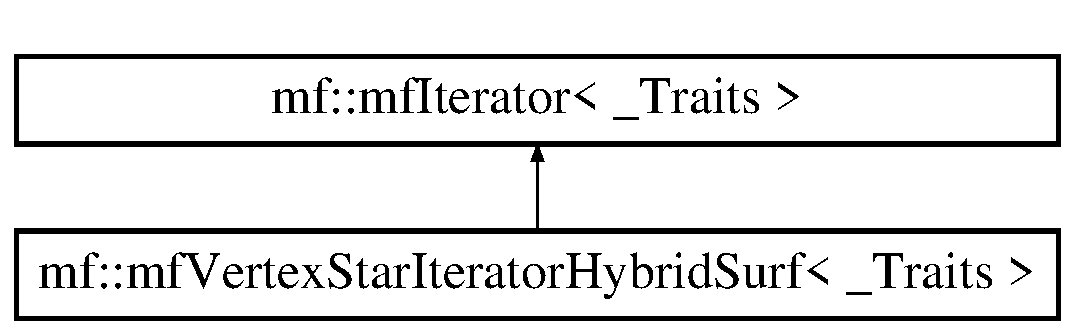
\includegraphics[height=2.000000cm]{classmf_1_1mfVertexStarIteratorHybridSurf}
\end{center}
\end{figure}
\subsection*{Public Types}
\begin{DoxyCompactItemize}
\item 
typedef \_\-Traits::sCell \hyperlink{classmf_1_1mfVertexStarIteratorHybridSurf_aae6c12237bca0c9f2b89ba3c4de79956}{sCell}
\item 
typedef \_\-Traits::sVertex \hyperlink{classmf_1_1mfVertexStarIteratorHybridSurf_af127643c84159641fa27dcae42d3827b}{sVertex}
\item 
typedef \_\-Traits::ids \hyperlink{classmf_1_1mfVertexStarIteratorHybridSurf_a32d570ad58eb0990e038c4058730d16e}{ids}
\item 
typedef \hyperlink{classmf_1_1mfSing}{mfSing}$<$ \_\-Traits $>$ \hyperlink{classmf_1_1mfVertexStarIteratorHybridSurf_ad9d3b4599b8c75447e1a84cc9fcade36}{sSing}
\item 
typedef \_\-Traits::sMesh \hyperlink{classmf_1_1mfVertexStarIteratorHybridSurf_a83c02395712edc51c7887c7256718c2c}{sMesh}
\end{DoxyCompactItemize}
\subsection*{Public Member Functions}
\begin{DoxyCompactItemize}
\item 
\hyperlink{classmf_1_1mfVertexStarIteratorHybridSurf_ae80cce93fa1363fa5e931d810709a29d}{mfVertexStarIteratorHybridSurf} (\hyperlink{classmf_1_1mfIterator_aca31e4d7e7eca4e3b100530d8725064b}{sMesh} $\ast$\_\-mesh)
\item 
\hyperlink{classmf_1_1mfVertexStarIteratorHybridSurf_a69afc45b1953abc8c655a9525fac8271}{$\sim$mfVertexStarIteratorHybridSurf} ()
\item 
\hypertarget{classmf_1_1mfVertexStarIteratorHybridSurf_a46c67a9d97a59e3cccf9615c3625cea7}{
bool {\bfseries initialize} (\hyperlink{classmf_1_1mfVertexStarIteratorHybridSurf_a32d570ad58eb0990e038c4058730d16e}{ids} init)}
\label{classmf_1_1mfVertexStarIteratorHybridSurf_a46c67a9d97a59e3cccf9615c3625cea7}

\item 
\hypertarget{classmf_1_1mfVertexStarIteratorHybridSurf_a953b50c222229dcdda5df1049041785a}{
bool {\bfseries finish} ()}
\label{classmf_1_1mfVertexStarIteratorHybridSurf_a953b50c222229dcdda5df1049041785a}

\item 
\hypertarget{classmf_1_1mfVertexStarIteratorHybridSurf_a38beb01c4a296c3de804ad9278a2af71}{
bool {\bfseries notFinish} ()}
\label{classmf_1_1mfVertexStarIteratorHybridSurf_a38beb01c4a296c3de804ad9278a2af71}

\item 
\hypertarget{classmf_1_1mfVertexStarIteratorHybridSurf_ae93169bac861a05b85120c215016c81f}{
bool {\bfseries operator++} ()}
\label{classmf_1_1mfVertexStarIteratorHybridSurf_ae93169bac861a05b85120c215016c81f}

\item 
\hypertarget{classmf_1_1mfVertexStarIteratorHybridSurf_af1a0a445f35458deb52a6cc770ec230e}{
\hyperlink{classmf_1_1mfVertexStarIteratorHybridSurf_aae6c12237bca0c9f2b89ba3c4de79956}{sCell} $\ast$ {\bfseries operator-\/$>$} ()}
\label{classmf_1_1mfVertexStarIteratorHybridSurf_af1a0a445f35458deb52a6cc770ec230e}

\item 
\hypertarget{classmf_1_1mfVertexStarIteratorHybridSurf_ab6664f69fba3212bb8918cc17ec506fa}{
\hyperlink{classmf_1_1mfVertexStarIteratorHybridSurf_aae6c12237bca0c9f2b89ba3c4de79956}{sCell} $\ast$ {\bfseries operator$\ast$} ()}
\label{classmf_1_1mfVertexStarIteratorHybridSurf_ab6664f69fba3212bb8918cc17ec506fa}

\item 
\hypertarget{classmf_1_1mfVertexStarIteratorHybridSurf_ad1eec61f6db2045615a1c4c35cf1016e}{
\hyperlink{classmf_1_1mfVertexStarIteratorHybridSurf_a32d570ad58eb0990e038c4058730d16e}{ids} {\bfseries operator\&} ()}
\label{classmf_1_1mfVertexStarIteratorHybridSurf_ad1eec61f6db2045615a1c4c35cf1016e}

\end{DoxyCompactItemize}
\subsubsection*{template$<$class \_\-Traits$>$ class mf::mfVertexStarIteratorHybridSurf$<$ \_\-Traits $>$}



\subsection{Member Typedef Documentation}
\hypertarget{classmf_1_1mfVertexStarIteratorHybridSurf_a32d570ad58eb0990e038c4058730d16e}{
\index{mf::mfVertexStarIteratorHybridSurf@{mf::mfVertexStarIteratorHybridSurf}!ids@{ids}}
\index{ids@{ids}!mf::mfVertexStarIteratorHybridSurf@{mf::mfVertexStarIteratorHybridSurf}}
\subsubsection[{ids}]{\setlength{\rightskip}{0pt plus 5cm}template$<$class \_\-Traits $>$ typedef \_\-Traits::ids {\bf mf::mfVertexStarIteratorHybridSurf}$<$ \_\-Traits $>$::{\bf ids}}}
\label{classmf_1_1mfVertexStarIteratorHybridSurf_a32d570ad58eb0990e038c4058730d16e}
Id typename definition \hypertarget{classmf_1_1mfVertexStarIteratorHybridSurf_aae6c12237bca0c9f2b89ba3c4de79956}{
\index{mf::mfVertexStarIteratorHybridSurf@{mf::mfVertexStarIteratorHybridSurf}!sCell@{sCell}}
\index{sCell@{sCell}!mf::mfVertexStarIteratorHybridSurf@{mf::mfVertexStarIteratorHybridSurf}}
\subsubsection[{sCell}]{\setlength{\rightskip}{0pt plus 5cm}template$<$class \_\-Traits $>$ typedef \_\-Traits::sCell {\bf mf::mfVertexStarIteratorHybridSurf}$<$ \_\-Traits $>$::{\bf sCell}}}
\label{classmf_1_1mfVertexStarIteratorHybridSurf_aae6c12237bca0c9f2b89ba3c4de79956}
Cell typename definition \hypertarget{classmf_1_1mfVertexStarIteratorHybridSurf_a83c02395712edc51c7887c7256718c2c}{
\index{mf::mfVertexStarIteratorHybridSurf@{mf::mfVertexStarIteratorHybridSurf}!sMesh@{sMesh}}
\index{sMesh@{sMesh}!mf::mfVertexStarIteratorHybridSurf@{mf::mfVertexStarIteratorHybridSurf}}
\subsubsection[{sMesh}]{\setlength{\rightskip}{0pt plus 5cm}template$<$class \_\-Traits $>$ typedef \_\-Traits::sMesh {\bf mf::mfVertexStarIteratorHybridSurf}$<$ \_\-Traits $>$::{\bf sMesh}}}
\label{classmf_1_1mfVertexStarIteratorHybridSurf_a83c02395712edc51c7887c7256718c2c}
Mesh typename definition 

Reimplemented from \hyperlink{classmf_1_1mfIterator_aca31e4d7e7eca4e3b100530d8725064b}{mf::mfIterator$<$ \_\-Traits $>$}.

\hypertarget{classmf_1_1mfVertexStarIteratorHybridSurf_ad9d3b4599b8c75447e1a84cc9fcade36}{
\index{mf::mfVertexStarIteratorHybridSurf@{mf::mfVertexStarIteratorHybridSurf}!sSing@{sSing}}
\index{sSing@{sSing}!mf::mfVertexStarIteratorHybridSurf@{mf::mfVertexStarIteratorHybridSurf}}
\subsubsection[{sSing}]{\setlength{\rightskip}{0pt plus 5cm}template$<$class \_\-Traits $>$ typedef {\bf mfSing}$<$\_\-Traits$>$ {\bf mf::mfVertexStarIteratorHybridSurf}$<$ \_\-Traits $>$::{\bf sSing}}}
\label{classmf_1_1mfVertexStarIteratorHybridSurf_ad9d3b4599b8c75447e1a84cc9fcade36}
Singular typename definition \hypertarget{classmf_1_1mfVertexStarIteratorHybridSurf_af127643c84159641fa27dcae42d3827b}{
\index{mf::mfVertexStarIteratorHybridSurf@{mf::mfVertexStarIteratorHybridSurf}!sVertex@{sVertex}}
\index{sVertex@{sVertex}!mf::mfVertexStarIteratorHybridSurf@{mf::mfVertexStarIteratorHybridSurf}}
\subsubsection[{sVertex}]{\setlength{\rightskip}{0pt plus 5cm}template$<$class \_\-Traits $>$ typedef \_\-Traits::sVertex {\bf mf::mfVertexStarIteratorHybridSurf}$<$ \_\-Traits $>$::{\bf sVertex}}}
\label{classmf_1_1mfVertexStarIteratorHybridSurf_af127643c84159641fa27dcae42d3827b}
Vertex typename definition 

\subsection{Constructor \& Destructor Documentation}
\hypertarget{classmf_1_1mfVertexStarIteratorHybridSurf_ae80cce93fa1363fa5e931d810709a29d}{
\index{mf::mfVertexStarIteratorHybridSurf@{mf::mfVertexStarIteratorHybridSurf}!mfVertexStarIteratorHybridSurf@{mfVertexStarIteratorHybridSurf}}
\index{mfVertexStarIteratorHybridSurf@{mfVertexStarIteratorHybridSurf}!mf::mfVertexStarIteratorHybridSurf@{mf::mfVertexStarIteratorHybridSurf}}
\subsubsection[{mfVertexStarIteratorHybridSurf}]{\setlength{\rightskip}{0pt plus 5cm}template$<$class \_\-Traits $>$ {\bf mf::mfVertexStarIteratorHybridSurf}$<$ \_\-Traits $>$::{\bf mfVertexStarIteratorHybridSurf} (
\begin{DoxyParamCaption}
\item[{{\bf sMesh} $\ast$}]{\_\-mesh}
\end{DoxyParamCaption}
)}}
\label{classmf_1_1mfVertexStarIteratorHybridSurf_ae80cce93fa1363fa5e931d810709a29d}
Construtor \hypertarget{classmf_1_1mfVertexStarIteratorHybridSurf_a69afc45b1953abc8c655a9525fac8271}{
\index{mf::mfVertexStarIteratorHybridSurf@{mf::mfVertexStarIteratorHybridSurf}!$\sim$mfVertexStarIteratorHybridSurf@{$\sim$mfVertexStarIteratorHybridSurf}}
\index{$\sim$mfVertexStarIteratorHybridSurf@{$\sim$mfVertexStarIteratorHybridSurf}!mf::mfVertexStarIteratorHybridSurf@{mf::mfVertexStarIteratorHybridSurf}}
\subsubsection[{$\sim$mfVertexStarIteratorHybridSurf}]{\setlength{\rightskip}{0pt plus 5cm}template$<$class \_\-Traits $>$ {\bf mf::mfVertexStarIteratorHybridSurf}$<$ \_\-Traits $>$::$\sim${\bf mfVertexStarIteratorHybridSurf} (
\begin{DoxyParamCaption}
{}
\end{DoxyParamCaption}
)}}
\label{classmf_1_1mfVertexStarIteratorHybridSurf_a69afc45b1953abc8c655a9525fac8271}
Destrutor 

The documentation for this class was generated from the following file:\begin{DoxyCompactItemize}
\item 
mfVertexStarIteratorHybridSurf.h\end{DoxyCompactItemize}

\hypertarget{classmf_1_1mfVertexStarIteratorQuadSurf}{
\section{mf::mfVertexStarIteratorQuadSurf$<$ \_\-Traits $>$ Class Template Reference}
\label{classmf_1_1mfVertexStarIteratorQuadSurf}\index{mf::mfVertexStarIteratorQuadSurf@{mf::mfVertexStarIteratorQuadSurf}}
}
Inheritance diagram for mf::mfVertexStarIteratorQuadSurf$<$ \_\-Traits $>$:\begin{figure}[H]
\begin{center}
\leavevmode
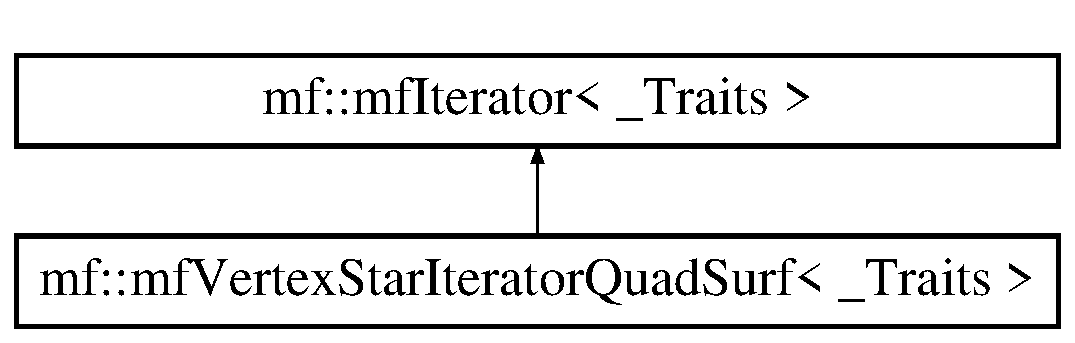
\includegraphics[height=2.000000cm]{classmf_1_1mfVertexStarIteratorQuadSurf}
\end{center}
\end{figure}
\subsection*{Public Types}
\begin{DoxyCompactItemize}
\item 
typedef \_\-Traits::sCell \hyperlink{classmf_1_1mfVertexStarIteratorQuadSurf_ae12c1c72db3d7cfc1240928080fa58f0}{sCell}
\item 
typedef \_\-Traits::sVertex \hyperlink{classmf_1_1mfVertexStarIteratorQuadSurf_ab31908dfd0f8e27af019e03d3771c0b8}{sVertex}
\item 
typedef \_\-Traits::ids \hyperlink{classmf_1_1mfVertexStarIteratorQuadSurf_a5c6de4cc45f4f21c3e30a4753fc9b22b}{ids}
\item 
typedef \hyperlink{classmf_1_1mfSing}{mfSing}$<$ \_\-Traits $>$ \hyperlink{classmf_1_1mfVertexStarIteratorQuadSurf_a8e91ca9813a3b27d6db68c9eb403ad77}{sSing}
\item 
typedef \_\-Traits::sMesh \hyperlink{classmf_1_1mfVertexStarIteratorQuadSurf_aad751ed48afa8c48bba2ed997bdd4676}{sMesh}
\end{DoxyCompactItemize}
\subsection*{Public Member Functions}
\begin{DoxyCompactItemize}
\item 
\hyperlink{classmf_1_1mfVertexStarIteratorQuadSurf_a0131aaf7181836f70c85037e67608ca2}{mfVertexStarIteratorQuadSurf} (\hyperlink{classmf_1_1mfIterator_aca31e4d7e7eca4e3b100530d8725064b}{sMesh} $\ast$\_\-mesh)
\item 
\hyperlink{classmf_1_1mfVertexStarIteratorQuadSurf_a4606fe32059583e8492f694c0ec731ac}{$\sim$mfVertexStarIteratorQuadSurf} ()
\item 
\hypertarget{classmf_1_1mfVertexStarIteratorQuadSurf_adf3c7bda7d1b65e14073a05ef0eec738}{
bool {\bfseries initialize} (\hyperlink{classmf_1_1mfVertexStarIteratorQuadSurf_a5c6de4cc45f4f21c3e30a4753fc9b22b}{ids} init)}
\label{classmf_1_1mfVertexStarIteratorQuadSurf_adf3c7bda7d1b65e14073a05ef0eec738}

\item 
\hypertarget{classmf_1_1mfVertexStarIteratorQuadSurf_a19123c5da7936b1455c4eb064361dbb8}{
bool {\bfseries finish} ()}
\label{classmf_1_1mfVertexStarIteratorQuadSurf_a19123c5da7936b1455c4eb064361dbb8}

\item 
\hypertarget{classmf_1_1mfVertexStarIteratorQuadSurf_a54730087113a77238c93f96b86f98057}{
bool {\bfseries notFinish} ()}
\label{classmf_1_1mfVertexStarIteratorQuadSurf_a54730087113a77238c93f96b86f98057}

\item 
\hypertarget{classmf_1_1mfVertexStarIteratorQuadSurf_a394c0432212e06f3705b167ffe8da1dd}{
bool {\bfseries operator++} ()}
\label{classmf_1_1mfVertexStarIteratorQuadSurf_a394c0432212e06f3705b167ffe8da1dd}

\item 
\hypertarget{classmf_1_1mfVertexStarIteratorQuadSurf_ad7fc6cf115dfb3ecb0698a1d7ce16441}{
\hyperlink{classmf_1_1mfVertexStarIteratorQuadSurf_ae12c1c72db3d7cfc1240928080fa58f0}{sCell} $\ast$ {\bfseries operator-\/$>$} ()}
\label{classmf_1_1mfVertexStarIteratorQuadSurf_ad7fc6cf115dfb3ecb0698a1d7ce16441}

\item 
\hypertarget{classmf_1_1mfVertexStarIteratorQuadSurf_a17ef846bbbb761fe69ee7113e16bd841}{
\hyperlink{classmf_1_1mfVertexStarIteratorQuadSurf_ae12c1c72db3d7cfc1240928080fa58f0}{sCell} $\ast$ {\bfseries operator$\ast$} ()}
\label{classmf_1_1mfVertexStarIteratorQuadSurf_a17ef846bbbb761fe69ee7113e16bd841}

\item 
\hypertarget{classmf_1_1mfVertexStarIteratorQuadSurf_a3960c401cc6b1c81dd4559b8e7b58f45}{
\hyperlink{classmf_1_1mfVertexStarIteratorQuadSurf_a5c6de4cc45f4f21c3e30a4753fc9b22b}{ids} {\bfseries operator\&} ()}
\label{classmf_1_1mfVertexStarIteratorQuadSurf_a3960c401cc6b1c81dd4559b8e7b58f45}

\end{DoxyCompactItemize}
\subsubsection*{template$<$class \_\-Traits$>$ class mf::mfVertexStarIteratorQuadSurf$<$ \_\-Traits $>$}



\subsection{Member Typedef Documentation}
\hypertarget{classmf_1_1mfVertexStarIteratorQuadSurf_a5c6de4cc45f4f21c3e30a4753fc9b22b}{
\index{mf::mfVertexStarIteratorQuadSurf@{mf::mfVertexStarIteratorQuadSurf}!ids@{ids}}
\index{ids@{ids}!mf::mfVertexStarIteratorQuadSurf@{mf::mfVertexStarIteratorQuadSurf}}
\subsubsection[{ids}]{\setlength{\rightskip}{0pt plus 5cm}template$<$class \_\-Traits $>$ typedef \_\-Traits::ids {\bf mf::mfVertexStarIteratorQuadSurf}$<$ \_\-Traits $>$::{\bf ids}}}
\label{classmf_1_1mfVertexStarIteratorQuadSurf_a5c6de4cc45f4f21c3e30a4753fc9b22b}
Id typename definition \hypertarget{classmf_1_1mfVertexStarIteratorQuadSurf_ae12c1c72db3d7cfc1240928080fa58f0}{
\index{mf::mfVertexStarIteratorQuadSurf@{mf::mfVertexStarIteratorQuadSurf}!sCell@{sCell}}
\index{sCell@{sCell}!mf::mfVertexStarIteratorQuadSurf@{mf::mfVertexStarIteratorQuadSurf}}
\subsubsection[{sCell}]{\setlength{\rightskip}{0pt plus 5cm}template$<$class \_\-Traits $>$ typedef \_\-Traits::sCell {\bf mf::mfVertexStarIteratorQuadSurf}$<$ \_\-Traits $>$::{\bf sCell}}}
\label{classmf_1_1mfVertexStarIteratorQuadSurf_ae12c1c72db3d7cfc1240928080fa58f0}
Cell typename definition \hypertarget{classmf_1_1mfVertexStarIteratorQuadSurf_aad751ed48afa8c48bba2ed997bdd4676}{
\index{mf::mfVertexStarIteratorQuadSurf@{mf::mfVertexStarIteratorQuadSurf}!sMesh@{sMesh}}
\index{sMesh@{sMesh}!mf::mfVertexStarIteratorQuadSurf@{mf::mfVertexStarIteratorQuadSurf}}
\subsubsection[{sMesh}]{\setlength{\rightskip}{0pt plus 5cm}template$<$class \_\-Traits $>$ typedef \_\-Traits::sMesh {\bf mf::mfVertexStarIteratorQuadSurf}$<$ \_\-Traits $>$::{\bf sMesh}}}
\label{classmf_1_1mfVertexStarIteratorQuadSurf_aad751ed48afa8c48bba2ed997bdd4676}
Mesh typename definition 

Reimplemented from \hyperlink{classmf_1_1mfIterator_aca31e4d7e7eca4e3b100530d8725064b}{mf::mfIterator$<$ \_\-Traits $>$}.

\hypertarget{classmf_1_1mfVertexStarIteratorQuadSurf_a8e91ca9813a3b27d6db68c9eb403ad77}{
\index{mf::mfVertexStarIteratorQuadSurf@{mf::mfVertexStarIteratorQuadSurf}!sSing@{sSing}}
\index{sSing@{sSing}!mf::mfVertexStarIteratorQuadSurf@{mf::mfVertexStarIteratorQuadSurf}}
\subsubsection[{sSing}]{\setlength{\rightskip}{0pt plus 5cm}template$<$class \_\-Traits $>$ typedef {\bf mfSing}$<$\_\-Traits$>$ {\bf mf::mfVertexStarIteratorQuadSurf}$<$ \_\-Traits $>$::{\bf sSing}}}
\label{classmf_1_1mfVertexStarIteratorQuadSurf_a8e91ca9813a3b27d6db68c9eb403ad77}
Singular typename definition \hypertarget{classmf_1_1mfVertexStarIteratorQuadSurf_ab31908dfd0f8e27af019e03d3771c0b8}{
\index{mf::mfVertexStarIteratorQuadSurf@{mf::mfVertexStarIteratorQuadSurf}!sVertex@{sVertex}}
\index{sVertex@{sVertex}!mf::mfVertexStarIteratorQuadSurf@{mf::mfVertexStarIteratorQuadSurf}}
\subsubsection[{sVertex}]{\setlength{\rightskip}{0pt plus 5cm}template$<$class \_\-Traits $>$ typedef \_\-Traits::sVertex {\bf mf::mfVertexStarIteratorQuadSurf}$<$ \_\-Traits $>$::{\bf sVertex}}}
\label{classmf_1_1mfVertexStarIteratorQuadSurf_ab31908dfd0f8e27af019e03d3771c0b8}
Vertex typename definition 

\subsection{Constructor \& Destructor Documentation}
\hypertarget{classmf_1_1mfVertexStarIteratorQuadSurf_a0131aaf7181836f70c85037e67608ca2}{
\index{mf::mfVertexStarIteratorQuadSurf@{mf::mfVertexStarIteratorQuadSurf}!mfVertexStarIteratorQuadSurf@{mfVertexStarIteratorQuadSurf}}
\index{mfVertexStarIteratorQuadSurf@{mfVertexStarIteratorQuadSurf}!mf::mfVertexStarIteratorQuadSurf@{mf::mfVertexStarIteratorQuadSurf}}
\subsubsection[{mfVertexStarIteratorQuadSurf}]{\setlength{\rightskip}{0pt plus 5cm}template$<$class \_\-Traits $>$ {\bf mf::mfVertexStarIteratorQuadSurf}$<$ \_\-Traits $>$::{\bf mfVertexStarIteratorQuadSurf} (
\begin{DoxyParamCaption}
\item[{{\bf sMesh} $\ast$}]{\_\-mesh}
\end{DoxyParamCaption}
)}}
\label{classmf_1_1mfVertexStarIteratorQuadSurf_a0131aaf7181836f70c85037e67608ca2}
Construtor \hypertarget{classmf_1_1mfVertexStarIteratorQuadSurf_a4606fe32059583e8492f694c0ec731ac}{
\index{mf::mfVertexStarIteratorQuadSurf@{mf::mfVertexStarIteratorQuadSurf}!$\sim$mfVertexStarIteratorQuadSurf@{$\sim$mfVertexStarIteratorQuadSurf}}
\index{$\sim$mfVertexStarIteratorQuadSurf@{$\sim$mfVertexStarIteratorQuadSurf}!mf::mfVertexStarIteratorQuadSurf@{mf::mfVertexStarIteratorQuadSurf}}
\subsubsection[{$\sim$mfVertexStarIteratorQuadSurf}]{\setlength{\rightskip}{0pt plus 5cm}template$<$class \_\-Traits $>$ {\bf mf::mfVertexStarIteratorQuadSurf}$<$ \_\-Traits $>$::$\sim${\bf mfVertexStarIteratorQuadSurf} (
\begin{DoxyParamCaption}
{}
\end{DoxyParamCaption}
)}}
\label{classmf_1_1mfVertexStarIteratorQuadSurf_a4606fe32059583e8492f694c0ec731ac}
Destrutor 

The documentation for this class was generated from the following file:\begin{DoxyCompactItemize}
\item 
mfVertexStarIteratorQuadSurf.h\end{DoxyCompactItemize}

\hypertarget{classmf_1_1mfVertexStarIteratorTetra}{
\section{mf::mfVertexStarIteratorTetra$<$ \_\-Traits $>$ Class Template Reference}
\label{classmf_1_1mfVertexStarIteratorTetra}\index{mf::mfVertexStarIteratorTetra@{mf::mfVertexStarIteratorTetra}}
}
Inheritance diagram for mf::mfVertexStarIteratorTetra$<$ \_\-Traits $>$:\begin{figure}[H]
\begin{center}
\leavevmode
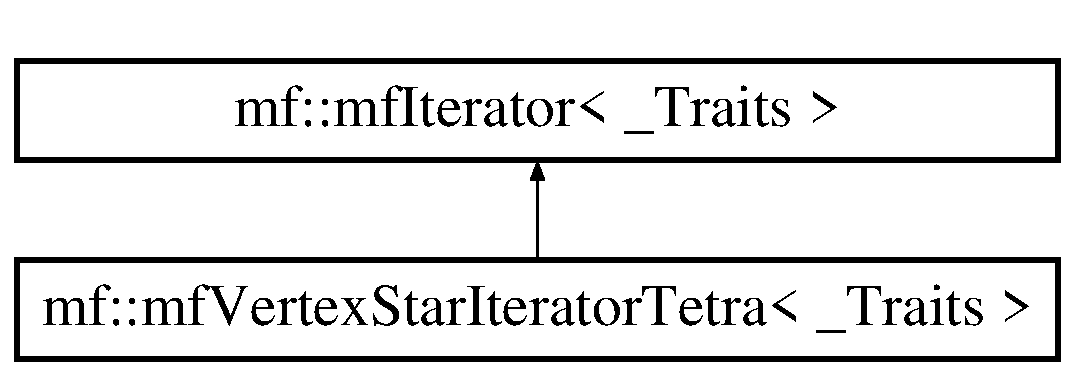
\includegraphics[height=2.000000cm]{classmf_1_1mfVertexStarIteratorTetra}
\end{center}
\end{figure}
\subsection*{Public Types}
\begin{DoxyCompactItemize}
\item 
\hypertarget{classmf_1_1mfVertexStarIteratorTetra_a73b533ca825ea973adc15f25152d7d21}{
typedef \_\-Traits::sCell {\bfseries sCell}}
\label{classmf_1_1mfVertexStarIteratorTetra_a73b533ca825ea973adc15f25152d7d21}

\item 
\hypertarget{classmf_1_1mfVertexStarIteratorTetra_a16b199793bc6d31a78eed3fffc6644bd}{
typedef \_\-Traits::sVertex {\bfseries sVertex}}
\label{classmf_1_1mfVertexStarIteratorTetra_a16b199793bc6d31a78eed3fffc6644bd}

\item 
\hypertarget{classmf_1_1mfVertexStarIteratorTetra_a2641fe9f6c4e8a3682d56887b55ecda5}{
typedef \_\-Traits::ids {\bfseries ids}}
\label{classmf_1_1mfVertexStarIteratorTetra_a2641fe9f6c4e8a3682d56887b55ecda5}

\item 
\hypertarget{classmf_1_1mfVertexStarIteratorTetra_adae62d5d7d040a360c62f8529fb156bc}{
typedef \hyperlink{classmf_1_1mfSing}{mfSing}$<$ \_\-Traits $>$ {\bfseries sSing}}
\label{classmf_1_1mfVertexStarIteratorTetra_adae62d5d7d040a360c62f8529fb156bc}

\item 
typedef \_\-Traits::sMesh \hyperlink{classmf_1_1mfVertexStarIteratorTetra_a19a9aafec3afbbafea712fa9c1a3417e}{sMesh}
\end{DoxyCompactItemize}
\subsection*{Public Member Functions}
\begin{DoxyCompactItemize}
\item 
\hyperlink{classmf_1_1mfVertexStarIteratorTetra_a390fe108ee096669cb97b675463dc108}{mfVertexStarIteratorTetra} (\hyperlink{classmf_1_1mfIterator_aca31e4d7e7eca4e3b100530d8725064b}{sMesh} $\ast$\_\-mesh)
\item 
\hyperlink{classmf_1_1mfVertexStarIteratorTetra_aa1016d2262cde5e8fc20a884bd73b672}{$\sim$mfVertexStarIteratorTetra} ()
\item 
\hypertarget{classmf_1_1mfVertexStarIteratorTetra_a654c6ec5fb4b32cd5ae596d0f27e5e13}{
bool {\bfseries initialize} (ids init)}
\label{classmf_1_1mfVertexStarIteratorTetra_a654c6ec5fb4b32cd5ae596d0f27e5e13}

\item 
\hypertarget{classmf_1_1mfVertexStarIteratorTetra_a183585661d0ee1a496608d63d8730075}{
bool {\bfseries finish} ()}
\label{classmf_1_1mfVertexStarIteratorTetra_a183585661d0ee1a496608d63d8730075}

\item 
\hypertarget{classmf_1_1mfVertexStarIteratorTetra_a37f6714f32884ded48627013ef1fa5a4}{
bool {\bfseries notFinish} ()}
\label{classmf_1_1mfVertexStarIteratorTetra_a37f6714f32884ded48627013ef1fa5a4}

\item 
\hypertarget{classmf_1_1mfVertexStarIteratorTetra_a7311e492ac00f08eb959a159472a515e}{
bool {\bfseries operator++} ()}
\label{classmf_1_1mfVertexStarIteratorTetra_a7311e492ac00f08eb959a159472a515e}

\item 
\hypertarget{classmf_1_1mfVertexStarIteratorTetra_af2ec5900b861bd61d2da85d8220127c4}{
sCell $\ast$ {\bfseries operator-\/$>$} ()}
\label{classmf_1_1mfVertexStarIteratorTetra_af2ec5900b861bd61d2da85d8220127c4}

\item 
\hypertarget{classmf_1_1mfVertexStarIteratorTetra_a6a368ce6afd8a49c2122ea738549bf6f}{
sCell $\ast$ {\bfseries operator$\ast$} ()}
\label{classmf_1_1mfVertexStarIteratorTetra_a6a368ce6afd8a49c2122ea738549bf6f}

\item 
\hypertarget{classmf_1_1mfVertexStarIteratorTetra_a79fdbcba50018db3cd181999d71da61d}{
ids {\bfseries operator\&} ()}
\label{classmf_1_1mfVertexStarIteratorTetra_a79fdbcba50018db3cd181999d71da61d}

\end{DoxyCompactItemize}
\subsubsection*{template$<$class \_\-Traits$>$ class mf::mfVertexStarIteratorTetra$<$ \_\-Traits $>$}



\subsection{Member Typedef Documentation}
\hypertarget{classmf_1_1mfVertexStarIteratorTetra_a19a9aafec3afbbafea712fa9c1a3417e}{
\index{mf::mfVertexStarIteratorTetra@{mf::mfVertexStarIteratorTetra}!sMesh@{sMesh}}
\index{sMesh@{sMesh}!mf::mfVertexStarIteratorTetra@{mf::mfVertexStarIteratorTetra}}
\subsubsection[{sMesh}]{\setlength{\rightskip}{0pt plus 5cm}template$<$class \_\-Traits $>$ typedef \_\-Traits::sMesh {\bf mf::mfVertexStarIteratorTetra}$<$ \_\-Traits $>$::{\bf sMesh}}}
\label{classmf_1_1mfVertexStarIteratorTetra_a19a9aafec3afbbafea712fa9c1a3417e}
Mesh typename definition 

Reimplemented from \hyperlink{classmf_1_1mfIterator_aca31e4d7e7eca4e3b100530d8725064b}{mf::mfIterator$<$ \_\-Traits $>$}.



\subsection{Constructor \& Destructor Documentation}
\hypertarget{classmf_1_1mfVertexStarIteratorTetra_a390fe108ee096669cb97b675463dc108}{
\index{mf::mfVertexStarIteratorTetra@{mf::mfVertexStarIteratorTetra}!mfVertexStarIteratorTetra@{mfVertexStarIteratorTetra}}
\index{mfVertexStarIteratorTetra@{mfVertexStarIteratorTetra}!mf::mfVertexStarIteratorTetra@{mf::mfVertexStarIteratorTetra}}
\subsubsection[{mfVertexStarIteratorTetra}]{\setlength{\rightskip}{0pt plus 5cm}template$<$class \_\-Traits $>$ {\bf mf::mfVertexStarIteratorTetra}$<$ \_\-Traits $>$::{\bf mfVertexStarIteratorTetra} (
\begin{DoxyParamCaption}
\item[{{\bf sMesh} $\ast$}]{\_\-mesh}
\end{DoxyParamCaption}
)}}
\label{classmf_1_1mfVertexStarIteratorTetra_a390fe108ee096669cb97b675463dc108}
Construtor \hypertarget{classmf_1_1mfVertexStarIteratorTetra_aa1016d2262cde5e8fc20a884bd73b672}{
\index{mf::mfVertexStarIteratorTetra@{mf::mfVertexStarIteratorTetra}!$\sim$mfVertexStarIteratorTetra@{$\sim$mfVertexStarIteratorTetra}}
\index{$\sim$mfVertexStarIteratorTetra@{$\sim$mfVertexStarIteratorTetra}!mf::mfVertexStarIteratorTetra@{mf::mfVertexStarIteratorTetra}}
\subsubsection[{$\sim$mfVertexStarIteratorTetra}]{\setlength{\rightskip}{0pt plus 5cm}template$<$class \_\-Traits $>$ {\bf mf::mfVertexStarIteratorTetra}$<$ \_\-Traits $>$::$\sim${\bf mfVertexStarIteratorTetra} (
\begin{DoxyParamCaption}
{}
\end{DoxyParamCaption}
)}}
\label{classmf_1_1mfVertexStarIteratorTetra_aa1016d2262cde5e8fc20a884bd73b672}
Destrutor 

The documentation for this class was generated from the following file:\begin{DoxyCompactItemize}
\item 
mfVertexStarIteratorTetra.h\end{DoxyCompactItemize}

\hypertarget{classmf_1_1mfVertexStarIteratorTriSurf}{
\section{mf::mfVertexStarIteratorTriSurf$<$ \_\-Traits $>$ Class Template Reference}
\label{classmf_1_1mfVertexStarIteratorTriSurf}\index{mf::mfVertexStarIteratorTriSurf@{mf::mfVertexStarIteratorTriSurf}}
}
Inheritance diagram for mf::mfVertexStarIteratorTriSurf$<$ \_\-Traits $>$:\begin{figure}[H]
\begin{center}
\leavevmode
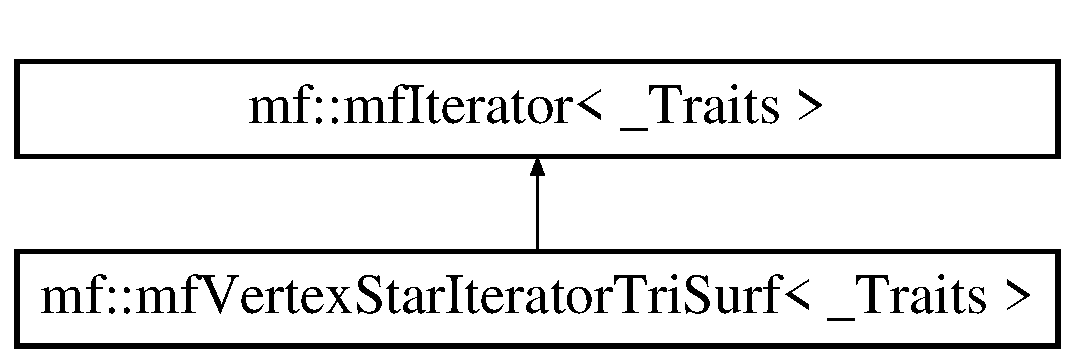
\includegraphics[height=2.000000cm]{classmf_1_1mfVertexStarIteratorTriSurf}
\end{center}
\end{figure}
\subsection*{Public Types}
\begin{DoxyCompactItemize}
\item 
typedef \_\-Traits::sCell \hyperlink{classmf_1_1mfVertexStarIteratorTriSurf_afe93e1a4572dfe24b7235db18ea90437}{sCell}
\item 
typedef \_\-Traits::sVertex \hyperlink{classmf_1_1mfVertexStarIteratorTriSurf_a2a1e281d8c7858e2e31d79a67d3884a3}{sVertex}
\item 
typedef \_\-Traits::ids \hyperlink{classmf_1_1mfVertexStarIteratorTriSurf_acd3a7e18747ad6cc0357bdd8fa366ac7}{ids}
\item 
typedef \hyperlink{classmf_1_1mfSing}{mfSing}$<$ \_\-Traits $>$ \hyperlink{classmf_1_1mfVertexStarIteratorTriSurf_a5fdb4a2a1f36e5069e68a1b0c6afdbd1}{sSing}
\item 
typedef \_\-Traits::sMesh \hyperlink{classmf_1_1mfVertexStarIteratorTriSurf_a6a0a8773d65d971e636d4361fb65b5af}{sMesh}
\end{DoxyCompactItemize}
\subsection*{Public Member Functions}
\begin{DoxyCompactItemize}
\item 
\hyperlink{classmf_1_1mfVertexStarIteratorTriSurf_a2075f3bb9affec4f91d432b2ffe83feb}{mfVertexStarIteratorTriSurf} (\hyperlink{classmf_1_1mfIterator_aca31e4d7e7eca4e3b100530d8725064b}{sMesh} $\ast$\_\-mesh)
\item 
\hyperlink{classmf_1_1mfVertexStarIteratorTriSurf_a517e91c7506e8f41856ee528f0ce4c0e}{$\sim$mfVertexStarIteratorTriSurf} ()
\item 
\hypertarget{classmf_1_1mfVertexStarIteratorTriSurf_a6023c1636cf9466cb18aca10e26dbd3a}{
bool {\bfseries initialize} (\hyperlink{classmf_1_1mfVertexStarIteratorTriSurf_acd3a7e18747ad6cc0357bdd8fa366ac7}{ids} init)}
\label{classmf_1_1mfVertexStarIteratorTriSurf_a6023c1636cf9466cb18aca10e26dbd3a}

\item 
\hypertarget{classmf_1_1mfVertexStarIteratorTriSurf_a7d4a452d3826de613f3e36db8f4f4e54}{
bool {\bfseries finish} ()}
\label{classmf_1_1mfVertexStarIteratorTriSurf_a7d4a452d3826de613f3e36db8f4f4e54}

\item 
\hypertarget{classmf_1_1mfVertexStarIteratorTriSurf_a3280cd14907a6f1e86605cd8e1e26485}{
bool {\bfseries notFinish} ()}
\label{classmf_1_1mfVertexStarIteratorTriSurf_a3280cd14907a6f1e86605cd8e1e26485}

\item 
\hypertarget{classmf_1_1mfVertexStarIteratorTriSurf_a39a3e8b216f012358d83a4a0d8f2f933}{
bool {\bfseries operator++} ()}
\label{classmf_1_1mfVertexStarIteratorTriSurf_a39a3e8b216f012358d83a4a0d8f2f933}

\item 
\hypertarget{classmf_1_1mfVertexStarIteratorTriSurf_a16af4d4a92a952fa243ccf51f59b6b7a}{
\hyperlink{classmf_1_1mfVertexStarIteratorTriSurf_afe93e1a4572dfe24b7235db18ea90437}{sCell} $\ast$ {\bfseries operator-\/$>$} ()}
\label{classmf_1_1mfVertexStarIteratorTriSurf_a16af4d4a92a952fa243ccf51f59b6b7a}

\item 
\hypertarget{classmf_1_1mfVertexStarIteratorTriSurf_a6a58839c393c39197aa342cae35f6ee3}{
\hyperlink{classmf_1_1mfVertexStarIteratorTriSurf_afe93e1a4572dfe24b7235db18ea90437}{sCell} $\ast$ {\bfseries operator$\ast$} ()}
\label{classmf_1_1mfVertexStarIteratorTriSurf_a6a58839c393c39197aa342cae35f6ee3}

\item 
\hypertarget{classmf_1_1mfVertexStarIteratorTriSurf_aad5fb05c7b6520068d9cffadabd22d86}{
\hyperlink{classmf_1_1mfVertexStarIteratorTriSurf_acd3a7e18747ad6cc0357bdd8fa366ac7}{ids} {\bfseries operator\&} ()}
\label{classmf_1_1mfVertexStarIteratorTriSurf_aad5fb05c7b6520068d9cffadabd22d86}

\end{DoxyCompactItemize}
\subsubsection*{template$<$class \_\-Traits$>$ class mf::mfVertexStarIteratorTriSurf$<$ \_\-Traits $>$}



\subsection{Member Typedef Documentation}
\hypertarget{classmf_1_1mfVertexStarIteratorTriSurf_acd3a7e18747ad6cc0357bdd8fa366ac7}{
\index{mf::mfVertexStarIteratorTriSurf@{mf::mfVertexStarIteratorTriSurf}!ids@{ids}}
\index{ids@{ids}!mf::mfVertexStarIteratorTriSurf@{mf::mfVertexStarIteratorTriSurf}}
\subsubsection[{ids}]{\setlength{\rightskip}{0pt plus 5cm}template$<$class \_\-Traits $>$ typedef \_\-Traits::ids {\bf mf::mfVertexStarIteratorTriSurf}$<$ \_\-Traits $>$::{\bf ids}}}
\label{classmf_1_1mfVertexStarIteratorTriSurf_acd3a7e18747ad6cc0357bdd8fa366ac7}
Id typename definition \hypertarget{classmf_1_1mfVertexStarIteratorTriSurf_afe93e1a4572dfe24b7235db18ea90437}{
\index{mf::mfVertexStarIteratorTriSurf@{mf::mfVertexStarIteratorTriSurf}!sCell@{sCell}}
\index{sCell@{sCell}!mf::mfVertexStarIteratorTriSurf@{mf::mfVertexStarIteratorTriSurf}}
\subsubsection[{sCell}]{\setlength{\rightskip}{0pt plus 5cm}template$<$class \_\-Traits $>$ typedef \_\-Traits::sCell {\bf mf::mfVertexStarIteratorTriSurf}$<$ \_\-Traits $>$::{\bf sCell}}}
\label{classmf_1_1mfVertexStarIteratorTriSurf_afe93e1a4572dfe24b7235db18ea90437}
Cell typename definition \hypertarget{classmf_1_1mfVertexStarIteratorTriSurf_a6a0a8773d65d971e636d4361fb65b5af}{
\index{mf::mfVertexStarIteratorTriSurf@{mf::mfVertexStarIteratorTriSurf}!sMesh@{sMesh}}
\index{sMesh@{sMesh}!mf::mfVertexStarIteratorTriSurf@{mf::mfVertexStarIteratorTriSurf}}
\subsubsection[{sMesh}]{\setlength{\rightskip}{0pt plus 5cm}template$<$class \_\-Traits $>$ typedef \_\-Traits::sMesh {\bf mf::mfVertexStarIteratorTriSurf}$<$ \_\-Traits $>$::{\bf sMesh}}}
\label{classmf_1_1mfVertexStarIteratorTriSurf_a6a0a8773d65d971e636d4361fb65b5af}
Mesh typename definition 

Reimplemented from \hyperlink{classmf_1_1mfIterator_aca31e4d7e7eca4e3b100530d8725064b}{mf::mfIterator$<$ \_\-Traits $>$}.

\hypertarget{classmf_1_1mfVertexStarIteratorTriSurf_a5fdb4a2a1f36e5069e68a1b0c6afdbd1}{
\index{mf::mfVertexStarIteratorTriSurf@{mf::mfVertexStarIteratorTriSurf}!sSing@{sSing}}
\index{sSing@{sSing}!mf::mfVertexStarIteratorTriSurf@{mf::mfVertexStarIteratorTriSurf}}
\subsubsection[{sSing}]{\setlength{\rightskip}{0pt plus 5cm}template$<$class \_\-Traits $>$ typedef {\bf mfSing}$<$\_\-Traits$>$ {\bf mf::mfVertexStarIteratorTriSurf}$<$ \_\-Traits $>$::{\bf sSing}}}
\label{classmf_1_1mfVertexStarIteratorTriSurf_a5fdb4a2a1f36e5069e68a1b0c6afdbd1}
Singular typename definition \hypertarget{classmf_1_1mfVertexStarIteratorTriSurf_a2a1e281d8c7858e2e31d79a67d3884a3}{
\index{mf::mfVertexStarIteratorTriSurf@{mf::mfVertexStarIteratorTriSurf}!sVertex@{sVertex}}
\index{sVertex@{sVertex}!mf::mfVertexStarIteratorTriSurf@{mf::mfVertexStarIteratorTriSurf}}
\subsubsection[{sVertex}]{\setlength{\rightskip}{0pt plus 5cm}template$<$class \_\-Traits $>$ typedef \_\-Traits::sVertex {\bf mf::mfVertexStarIteratorTriSurf}$<$ \_\-Traits $>$::{\bf sVertex}}}
\label{classmf_1_1mfVertexStarIteratorTriSurf_a2a1e281d8c7858e2e31d79a67d3884a3}
Vertex typename definition 

\subsection{Constructor \& Destructor Documentation}
\hypertarget{classmf_1_1mfVertexStarIteratorTriSurf_a2075f3bb9affec4f91d432b2ffe83feb}{
\index{mf::mfVertexStarIteratorTriSurf@{mf::mfVertexStarIteratorTriSurf}!mfVertexStarIteratorTriSurf@{mfVertexStarIteratorTriSurf}}
\index{mfVertexStarIteratorTriSurf@{mfVertexStarIteratorTriSurf}!mf::mfVertexStarIteratorTriSurf@{mf::mfVertexStarIteratorTriSurf}}
\subsubsection[{mfVertexStarIteratorTriSurf}]{\setlength{\rightskip}{0pt plus 5cm}template$<$class \_\-Traits $>$ {\bf mf::mfVertexStarIteratorTriSurf}$<$ \_\-Traits $>$::{\bf mfVertexStarIteratorTriSurf} (
\begin{DoxyParamCaption}
\item[{{\bf sMesh} $\ast$}]{\_\-mesh}
\end{DoxyParamCaption}
)}}
\label{classmf_1_1mfVertexStarIteratorTriSurf_a2075f3bb9affec4f91d432b2ffe83feb}
Construtor \hypertarget{classmf_1_1mfVertexStarIteratorTriSurf_a517e91c7506e8f41856ee528f0ce4c0e}{
\index{mf::mfVertexStarIteratorTriSurf@{mf::mfVertexStarIteratorTriSurf}!$\sim$mfVertexStarIteratorTriSurf@{$\sim$mfVertexStarIteratorTriSurf}}
\index{$\sim$mfVertexStarIteratorTriSurf@{$\sim$mfVertexStarIteratorTriSurf}!mf::mfVertexStarIteratorTriSurf@{mf::mfVertexStarIteratorTriSurf}}
\subsubsection[{$\sim$mfVertexStarIteratorTriSurf}]{\setlength{\rightskip}{0pt plus 5cm}template$<$class \_\-Traits $>$ {\bf mf::mfVertexStarIteratorTriSurf}$<$ \_\-Traits $>$::$\sim${\bf mfVertexStarIteratorTriSurf} (
\begin{DoxyParamCaption}
{}
\end{DoxyParamCaption}
)}}
\label{classmf_1_1mfVertexStarIteratorTriSurf_a517e91c7506e8f41856ee528f0ce4c0e}
Destrutor 

The documentation for this class was generated from the following file:\begin{DoxyCompactItemize}
\item 
mfVertexStarIteratorTriSurf.h\end{DoxyCompactItemize}

\hypertarget{classmf_1_1mfVerticesIterator}{
\section{mf::mfVerticesIterator$<$ \_\-Traits $>$ Class Template Reference}
\label{classmf_1_1mfVerticesIterator}\index{mf::mfVerticesIterator@{mf::mfVerticesIterator}}
}
Inheritance diagram for mf::mfVerticesIterator$<$ \_\-Traits $>$:\begin{figure}[H]
\begin{center}
\leavevmode
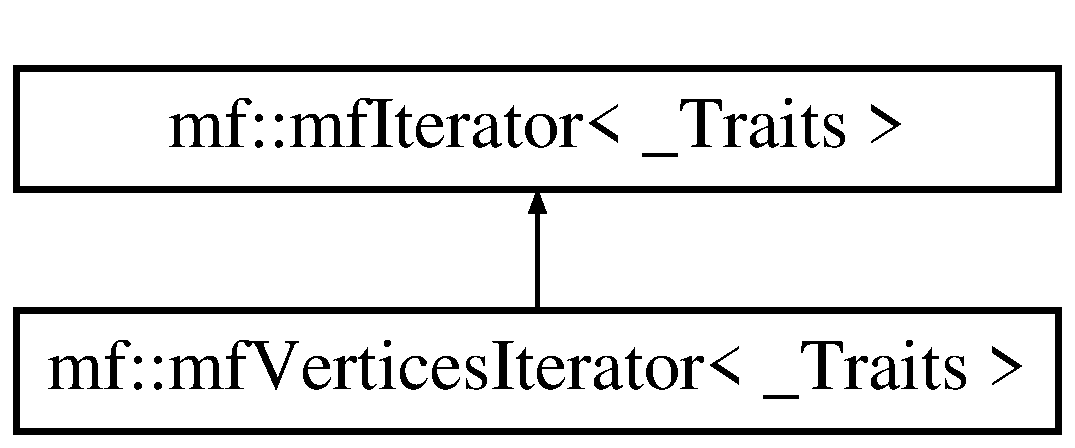
\includegraphics[height=2.000000cm]{classmf_1_1mfVerticesIterator}
\end{center}
\end{figure}
\subsection*{Public Types}
\begin{DoxyCompactItemize}
\item 
typedef \_\-Traits::sVertex \hyperlink{classmf_1_1mfVerticesIterator_a123ec8591eb79091da3c80bd1a3e2eca}{sVertex}
\item 
typedef \_\-Traits::ids \hyperlink{classmf_1_1mfVerticesIterator_a4d1c60d2572a77d4d5080b78c12a85f9}{ids}
\item 
typedef \_\-Traits::sMesh \hyperlink{classmf_1_1mfVerticesIterator_a351a7fef8c19f4cb57f4c0a68d337679}{sMesh}
\end{DoxyCompactItemize}
\subsection*{Public Member Functions}
\begin{DoxyCompactItemize}
\item 
\hyperlink{classmf_1_1mfVerticesIterator_a36cbafd47cdb27c54818973e05c00980}{mfVerticesIterator} (\hyperlink{classmf_1_1mfIterator_aca31e4d7e7eca4e3b100530d8725064b}{sMesh} $\ast$\_\-mesh)
\item 
\hyperlink{classmf_1_1mfVerticesIterator_a7de7fcdee6809c4857f0bccc02d7a4f8}{$\sim$mfVerticesIterator} ()
\item 
bool \hyperlink{classmf_1_1mfVerticesIterator_adde577253cf69727e98f913bc7659708}{initialize} (\hyperlink{classmf_1_1mfVerticesIterator_a4d1c60d2572a77d4d5080b78c12a85f9}{ids} init=0)
\item 
bool \hyperlink{classmf_1_1mfVerticesIterator_a28ce74d7e0a4eee32331385c0e45233f}{finish} ()
\item 
bool \hyperlink{classmf_1_1mfVerticesIterator_acccbff29ca7d53358a3f3d799e449e53}{notFinish} ()
\item 
\hypertarget{classmf_1_1mfVerticesIterator_a312576304811b3bc77b4f10a71c5c859}{
bool {\bfseries operator++} ()}
\label{classmf_1_1mfVerticesIterator_a312576304811b3bc77b4f10a71c5c859}

\item 
\hypertarget{classmf_1_1mfVerticesIterator_af1cc2b9f8aeb01f5b1563cbbe972af88}{
bool {\bfseries operator-\/-\/} ()}
\label{classmf_1_1mfVerticesIterator_af1cc2b9f8aeb01f5b1563cbbe972af88}

\item 
\hypertarget{classmf_1_1mfVerticesIterator_acd200563c161e01e67c425263c7c1f35}{
\hyperlink{classmf_1_1mfVerticesIterator_a123ec8591eb79091da3c80bd1a3e2eca}{sVertex} $\ast$ {\bfseries operator-\/$>$} ()}
\label{classmf_1_1mfVerticesIterator_acd200563c161e01e67c425263c7c1f35}

\item 
\hypertarget{classmf_1_1mfVerticesIterator_a6bcaaab59811acc32889a83e4b664e19}{
\hyperlink{classmf_1_1mfVerticesIterator_a123ec8591eb79091da3c80bd1a3e2eca}{sVertex} $\ast$ {\bfseries operator$\ast$} ()}
\label{classmf_1_1mfVerticesIterator_a6bcaaab59811acc32889a83e4b664e19}

\item 
\hyperlink{classmf_1_1mfVerticesIterator_a4d1c60d2572a77d4d5080b78c12a85f9}{ids} \hyperlink{classmf_1_1mfVerticesIterator_a21fd0fbb11a160d5754963f4de6e9b42}{operator\&} ()
\end{DoxyCompactItemize}
\subsubsection*{template$<$class \_\-Traits$>$ class mf::mfVerticesIterator$<$ \_\-Traits $>$}



\subsection{Member Typedef Documentation}
\hypertarget{classmf_1_1mfVerticesIterator_a4d1c60d2572a77d4d5080b78c12a85f9}{
\index{mf::mfVerticesIterator@{mf::mfVerticesIterator}!ids@{ids}}
\index{ids@{ids}!mf::mfVerticesIterator@{mf::mfVerticesIterator}}
\subsubsection[{ids}]{\setlength{\rightskip}{0pt plus 5cm}template$<$class \_\-Traits$>$ typedef \_\-Traits::ids {\bf mf::mfVerticesIterator}$<$ \_\-Traits $>$::{\bf ids}}}
\label{classmf_1_1mfVerticesIterator_a4d1c60d2572a77d4d5080b78c12a85f9}
Id typename definition \hypertarget{classmf_1_1mfVerticesIterator_a351a7fef8c19f4cb57f4c0a68d337679}{
\index{mf::mfVerticesIterator@{mf::mfVerticesIterator}!sMesh@{sMesh}}
\index{sMesh@{sMesh}!mf::mfVerticesIterator@{mf::mfVerticesIterator}}
\subsubsection[{sMesh}]{\setlength{\rightskip}{0pt plus 5cm}template$<$class \_\-Traits$>$ typedef \_\-Traits::sMesh {\bf mf::mfVerticesIterator}$<$ \_\-Traits $>$::{\bf sMesh}}}
\label{classmf_1_1mfVerticesIterator_a351a7fef8c19f4cb57f4c0a68d337679}
Mesh typename definition 

Reimplemented from \hyperlink{classmf_1_1mfIterator_aca31e4d7e7eca4e3b100530d8725064b}{mf::mfIterator$<$ \_\-Traits $>$}.

\hypertarget{classmf_1_1mfVerticesIterator_a123ec8591eb79091da3c80bd1a3e2eca}{
\index{mf::mfVerticesIterator@{mf::mfVerticesIterator}!sVertex@{sVertex}}
\index{sVertex@{sVertex}!mf::mfVerticesIterator@{mf::mfVerticesIterator}}
\subsubsection[{sVertex}]{\setlength{\rightskip}{0pt plus 5cm}template$<$class \_\-Traits$>$ typedef \_\-Traits::sVertex {\bf mf::mfVerticesIterator}$<$ \_\-Traits $>$::{\bf sVertex}}}
\label{classmf_1_1mfVerticesIterator_a123ec8591eb79091da3c80bd1a3e2eca}
Vertex typename definition 

\subsection{Constructor \& Destructor Documentation}
\hypertarget{classmf_1_1mfVerticesIterator_a36cbafd47cdb27c54818973e05c00980}{
\index{mf::mfVerticesIterator@{mf::mfVerticesIterator}!mfVerticesIterator@{mfVerticesIterator}}
\index{mfVerticesIterator@{mfVerticesIterator}!mf::mfVerticesIterator@{mf::mfVerticesIterator}}
\subsubsection[{mfVerticesIterator}]{\setlength{\rightskip}{0pt plus 5cm}template$<$class \_\-Traits $>$ {\bf mf::mfVerticesIterator}$<$ \_\-Traits $>$::{\bf mfVerticesIterator} (
\begin{DoxyParamCaption}
\item[{{\bf sMesh} $\ast$}]{\_\-mesh}
\end{DoxyParamCaption}
)}}
\label{classmf_1_1mfVerticesIterator_a36cbafd47cdb27c54818973e05c00980}
Construtor \hypertarget{classmf_1_1mfVerticesIterator_a7de7fcdee6809c4857f0bccc02d7a4f8}{
\index{mf::mfVerticesIterator@{mf::mfVerticesIterator}!$\sim$mfVerticesIterator@{$\sim$mfVerticesIterator}}
\index{$\sim$mfVerticesIterator@{$\sim$mfVerticesIterator}!mf::mfVerticesIterator@{mf::mfVerticesIterator}}
\subsubsection[{$\sim$mfVerticesIterator}]{\setlength{\rightskip}{0pt plus 5cm}template$<$class \_\-Traits $>$ {\bf mf::mfVerticesIterator}$<$ \_\-Traits $>$::$\sim${\bf mfVerticesIterator} (
\begin{DoxyParamCaption}
{}
\end{DoxyParamCaption}
)}}
\label{classmf_1_1mfVerticesIterator_a7de7fcdee6809c4857f0bccc02d7a4f8}
Destrutor 

\subsection{Member Function Documentation}
\hypertarget{classmf_1_1mfVerticesIterator_a28ce74d7e0a4eee32331385c0e45233f}{
\index{mf::mfVerticesIterator@{mf::mfVerticesIterator}!finish@{finish}}
\index{finish@{finish}!mf::mfVerticesIterator@{mf::mfVerticesIterator}}
\subsubsection[{finish}]{\setlength{\rightskip}{0pt plus 5cm}template$<$class \_\-Traits $>$ bool {\bf mf::mfVerticesIterator}$<$ \_\-Traits $>$::finish (
\begin{DoxyParamCaption}
{}
\end{DoxyParamCaption}
)}}
\label{classmf_1_1mfVerticesIterator_a28ce74d7e0a4eee32331385c0e45233f}
Determines if iterator is at the end of the vertex vector \hypertarget{classmf_1_1mfVerticesIterator_adde577253cf69727e98f913bc7659708}{
\index{mf::mfVerticesIterator@{mf::mfVerticesIterator}!initialize@{initialize}}
\index{initialize@{initialize}!mf::mfVerticesIterator@{mf::mfVerticesIterator}}
\subsubsection[{initialize}]{\setlength{\rightskip}{0pt plus 5cm}template$<$class \_\-Traits $>$ bool {\bf mf::mfVerticesIterator}$<$ \_\-Traits $>$::initialize (
\begin{DoxyParamCaption}
\item[{{\bf ids}}]{init = {\ttfamily 0}}
\end{DoxyParamCaption}
)}}
\label{classmf_1_1mfVerticesIterator_adde577253cf69727e98f913bc7659708}
Initializes the iterator at a determined position


\begin{DoxyParams}{Parameters}
{\em init,:} & initial position of the iterator (0 by default) \\
\hline
\end{DoxyParams}
\begin{DoxyReturn}{Returns}
true if the iterator is correctly initialized 
\end{DoxyReturn}
\hypertarget{classmf_1_1mfVerticesIterator_acccbff29ca7d53358a3f3d799e449e53}{
\index{mf::mfVerticesIterator@{mf::mfVerticesIterator}!notFinish@{notFinish}}
\index{notFinish@{notFinish}!mf::mfVerticesIterator@{mf::mfVerticesIterator}}
\subsubsection[{notFinish}]{\setlength{\rightskip}{0pt plus 5cm}template$<$class \_\-Traits $>$ bool {\bf mf::mfVerticesIterator}$<$ \_\-Traits $>$::notFinish (
\begin{DoxyParamCaption}
{}
\end{DoxyParamCaption}
)}}
\label{classmf_1_1mfVerticesIterator_acccbff29ca7d53358a3f3d799e449e53}
Determines if iterator isn't at the end of the vertex vector \hypertarget{classmf_1_1mfVerticesIterator_a21fd0fbb11a160d5754963f4de6e9b42}{
\index{mf::mfVerticesIterator@{mf::mfVerticesIterator}!operator\&@{operator\&}}
\index{operator\&@{operator\&}!mf::mfVerticesIterator@{mf::mfVerticesIterator}}
\subsubsection[{operator\&}]{\setlength{\rightskip}{0pt plus 5cm}template$<$class \_\-Traits $>$ IDS {\bf mf::mfVerticesIterator}$<$ \_\-Traits $>$::operator\& (
\begin{DoxyParamCaption}
{}
\end{DoxyParamCaption}
)}}
\label{classmf_1_1mfVerticesIterator_a21fd0fbb11a160d5754963f4de6e9b42}
Operator that returns the id of the current vertex 

The documentation for this class was generated from the following file:\begin{DoxyCompactItemize}
\item 
\hyperlink{mfVerticesIterator_8h}{mfVerticesIterator.h}\end{DoxyCompactItemize}

\hypertarget{classmf_1_1mfVtkReader}{
\section{mf::mfVtkReader$<$ \_\-Traits $>$ Class Template Reference}
\label{classmf_1_1mfVtkReader}\index{mf::mfVtkReader@{mf::mfVtkReader}}
}
Inheritance diagram for mf::mfVtkReader$<$ \_\-Traits $>$:\begin{figure}[H]
\begin{center}
\leavevmode
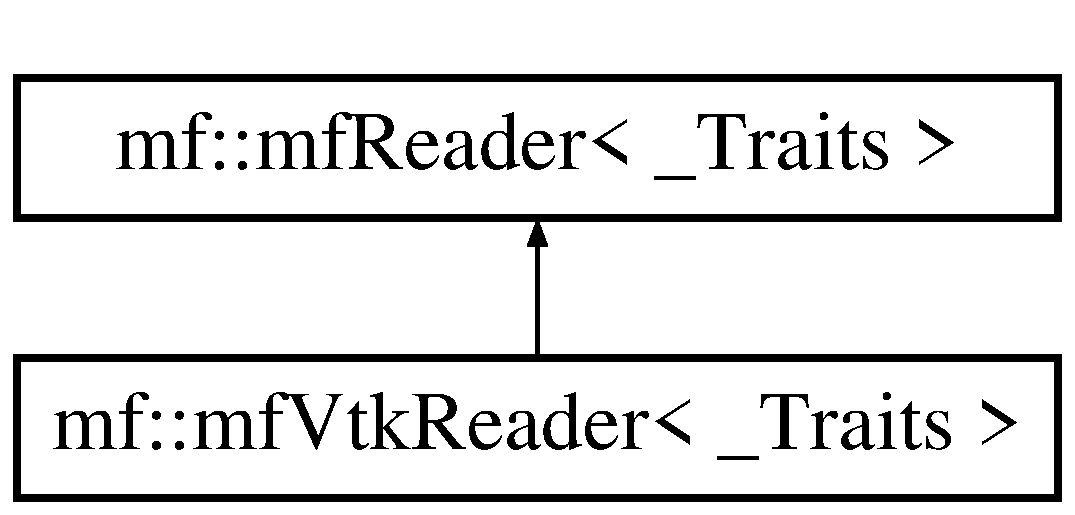
\includegraphics[height=2.000000cm]{classmf_1_1mfVtkReader}
\end{center}
\end{figure}
\subsection*{Public Types}
\begin{DoxyCompactItemize}
\item 
typedef \_\-Traits::space \hyperlink{classmf_1_1mfVtkReader_a157b4bcf691cc34e5333e4ff0b8976ad}{space}
\item 
typedef \_\-Traits::ids \hyperlink{classmf_1_1mfVtkReader_ad563f3eceaac2a5928f9f2cca98d8a64}{ids}
\item 
typedef \_\-Traits::sVertex \hyperlink{classmf_1_1mfVtkReader_a953ce52269ccebd0abb7f15147de46b3}{sVertex}
\item 
typedef \_\-Traits::sCell \hyperlink{classmf_1_1mfVtkReader_aa5070471f8c7bbc67628f91022ca06c9}{sCell}
\item 
typedef \_\-Traits::sMesh \hyperlink{classmf_1_1mfVtkReader_a21c487f2b456bef55115cf06620a2f3b}{sMesh}
\end{DoxyCompactItemize}
\subsection*{Public Member Functions}
\begin{DoxyCompactItemize}
\item 
\hyperlink{classmf_1_1mfVtkReader_ad42ee66b44197472cdeab9adea56b90b}{mfVtkReader} ()
\item 
\hyperlink{classmf_1_1mfVtkReader_abd8f5f738472810d3ec93f38b10193eb}{$\sim$mfVtkReader} ()
\item 
virtual bool \hyperlink{classmf_1_1mfVtkReader_a3cbb607039dd5acf5aa0071f8ee49786}{read} (\hyperlink{classmf_1_1mfVtkReader_a21c487f2b456bef55115cf06620a2f3b}{sMesh} $\ast$malha, const char $\ast$filename)
\begin{DoxyCompactList}\small\item\em Executa a leitura de um arquivo. \item\end{DoxyCompactList}\end{DoxyCompactItemize}
\subsubsection*{template$<$class \_\-Traits$>$ class mf::mfVtkReader$<$ \_\-Traits $>$}



\subsection{Member Typedef Documentation}
\hypertarget{classmf_1_1mfVtkReader_ad563f3eceaac2a5928f9f2cca98d8a64}{
\index{mf::mfVtkReader@{mf::mfVtkReader}!ids@{ids}}
\index{ids@{ids}!mf::mfVtkReader@{mf::mfVtkReader}}
\subsubsection[{ids}]{\setlength{\rightskip}{0pt plus 5cm}template$<$class \_\-Traits $>$ typedef \_\-Traits::ids {\bf mf::mfVtkReader}$<$ \_\-Traits $>$::{\bf ids}}}
\label{classmf_1_1mfVtkReader_ad563f3eceaac2a5928f9f2cca98d8a64}
Id typename definition \hypertarget{classmf_1_1mfVtkReader_aa5070471f8c7bbc67628f91022ca06c9}{
\index{mf::mfVtkReader@{mf::mfVtkReader}!sCell@{sCell}}
\index{sCell@{sCell}!mf::mfVtkReader@{mf::mfVtkReader}}
\subsubsection[{sCell}]{\setlength{\rightskip}{0pt plus 5cm}template$<$class \_\-Traits $>$ typedef \_\-Traits::sCell {\bf mf::mfVtkReader}$<$ \_\-Traits $>$::{\bf sCell}}}
\label{classmf_1_1mfVtkReader_aa5070471f8c7bbc67628f91022ca06c9}
Cell typename definition \hypertarget{classmf_1_1mfVtkReader_a21c487f2b456bef55115cf06620a2f3b}{
\index{mf::mfVtkReader@{mf::mfVtkReader}!sMesh@{sMesh}}
\index{sMesh@{sMesh}!mf::mfVtkReader@{mf::mfVtkReader}}
\subsubsection[{sMesh}]{\setlength{\rightskip}{0pt plus 5cm}template$<$class \_\-Traits $>$ typedef \_\-Traits::sMesh {\bf mf::mfVtkReader}$<$ \_\-Traits $>$::{\bf sMesh}}}
\label{classmf_1_1mfVtkReader_a21c487f2b456bef55115cf06620a2f3b}
Mesh typename definition 

Reimplemented from \hyperlink{classmf_1_1mfReader}{mf::mfReader$<$ \_\-Traits $>$}.

\hypertarget{classmf_1_1mfVtkReader_a157b4bcf691cc34e5333e4ff0b8976ad}{
\index{mf::mfVtkReader@{mf::mfVtkReader}!space@{space}}
\index{space@{space}!mf::mfVtkReader@{mf::mfVtkReader}}
\subsubsection[{space}]{\setlength{\rightskip}{0pt plus 5cm}template$<$class \_\-Traits $>$ typedef \_\-Traits::space {\bf mf::mfVtkReader}$<$ \_\-Traits $>$::{\bf space}}}
\label{classmf_1_1mfVtkReader_a157b4bcf691cc34e5333e4ff0b8976ad}
Space typename definition \hypertarget{classmf_1_1mfVtkReader_a953ce52269ccebd0abb7f15147de46b3}{
\index{mf::mfVtkReader@{mf::mfVtkReader}!sVertex@{sVertex}}
\index{sVertex@{sVertex}!mf::mfVtkReader@{mf::mfVtkReader}}
\subsubsection[{sVertex}]{\setlength{\rightskip}{0pt plus 5cm}template$<$class \_\-Traits $>$ typedef \_\-Traits::sVertex {\bf mf::mfVtkReader}$<$ \_\-Traits $>$::{\bf sVertex}}}
\label{classmf_1_1mfVtkReader_a953ce52269ccebd0abb7f15147de46b3}
Vertex typename definition 

\subsection{Constructor \& Destructor Documentation}
\hypertarget{classmf_1_1mfVtkReader_ad42ee66b44197472cdeab9adea56b90b}{
\index{mf::mfVtkReader@{mf::mfVtkReader}!mfVtkReader@{mfVtkReader}}
\index{mfVtkReader@{mfVtkReader}!mf::mfVtkReader@{mf::mfVtkReader}}
\subsubsection[{mfVtkReader}]{\setlength{\rightskip}{0pt plus 5cm}template$<$class \_\-Traits $>$ {\bf mf::mfVtkReader}$<$ \_\-Traits $>$::{\bf mfVtkReader} (
\begin{DoxyParamCaption}
{}
\end{DoxyParamCaption}
)}}
\label{classmf_1_1mfVtkReader_ad42ee66b44197472cdeab9adea56b90b}
Constructor \hypertarget{classmf_1_1mfVtkReader_abd8f5f738472810d3ec93f38b10193eb}{
\index{mf::mfVtkReader@{mf::mfVtkReader}!$\sim$mfVtkReader@{$\sim$mfVtkReader}}
\index{$\sim$mfVtkReader@{$\sim$mfVtkReader}!mf::mfVtkReader@{mf::mfVtkReader}}
\subsubsection[{$\sim$mfVtkReader}]{\setlength{\rightskip}{0pt plus 5cm}template$<$class \_\-Traits $>$ {\bf mf::mfVtkReader}$<$ \_\-Traits $>$::$\sim${\bf mfVtkReader} (
\begin{DoxyParamCaption}
{}
\end{DoxyParamCaption}
)}}
\label{classmf_1_1mfVtkReader_abd8f5f738472810d3ec93f38b10193eb}
Destructor 

\subsection{Member Function Documentation}
\hypertarget{classmf_1_1mfVtkReader_a3cbb607039dd5acf5aa0071f8ee49786}{
\index{mf::mfVtkReader@{mf::mfVtkReader}!read@{read}}
\index{read@{read}!mf::mfVtkReader@{mf::mfVtkReader}}
\subsubsection[{read}]{\setlength{\rightskip}{0pt plus 5cm}template$<$class \_\-Traits $>$ bool {\bf mf::mfVtkReader}$<$ \_\-Traits $>$::read (
\begin{DoxyParamCaption}
\item[{{\bf sMesh} $\ast$}]{malha, }
\item[{const char $\ast$}]{filename}
\end{DoxyParamCaption}
)\hspace{0.3cm}{\ttfamily  \mbox{[}virtual\mbox{]}}}}
\label{classmf_1_1mfVtkReader_a3cbb607039dd5acf5aa0071f8ee49786}


Executa a leitura de um arquivo. 

Paraetros de entrada: malha : endereco de memoria de destino da malha a ser carregada. Ja deve estar alocado. filename : nome do arquivo da malha. 

Implements \hyperlink{classmf_1_1mfReader_a0e0c3224a06b06a8fb82be4f0f4a2e00}{mf::mfReader$<$ \_\-Traits $>$}.



The documentation for this class was generated from the following file:\begin{DoxyCompactItemize}
\item 
mfVtkReader.h\end{DoxyCompactItemize}

\hypertarget{classmf_1_1mfVtkWriter}{
\section{mf::mfVtkWriter$<$ \_\-Traits $>$ Class Template Reference}
\label{classmf_1_1mfVtkWriter}\index{mf::mfVtkWriter@{mf::mfVtkWriter}}
}


Salva malhas em arquivo do tipo VTK sem dados.  




{\ttfamily \#include $<$mfVtkWriter.h$>$}

Inheritance diagram for mf::mfVtkWriter$<$ \_\-Traits $>$:\begin{figure}[H]
\begin{center}
\leavevmode
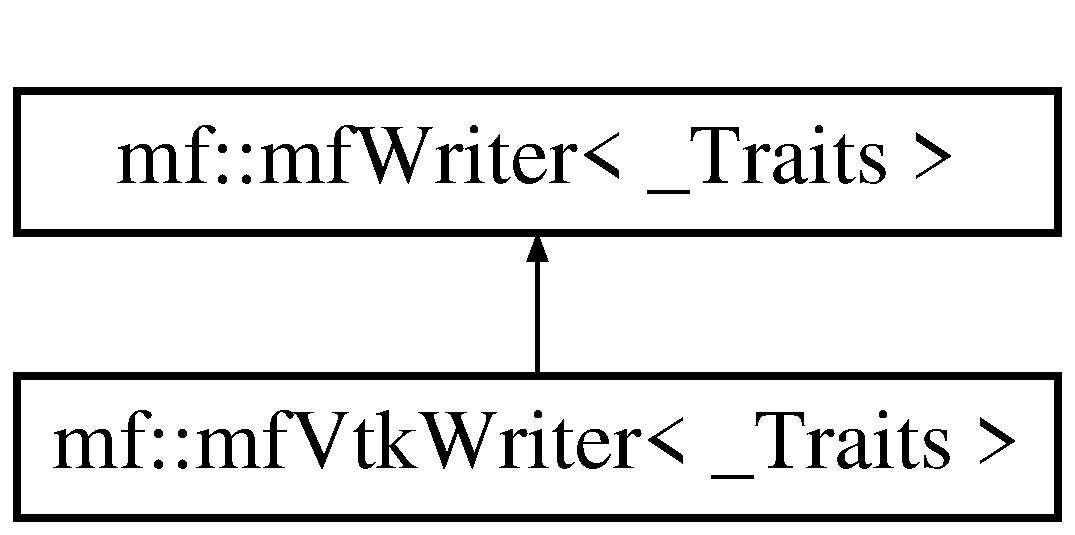
\includegraphics[height=2.000000cm]{classmf_1_1mfVtkWriter}
\end{center}
\end{figure}
\subsection*{Public Types}
\begin{DoxyCompactItemize}
\item 
typedef \_\-Traits::space \hyperlink{classmf_1_1mfVtkWriter_ad618b138c53f1ac5faf9d2221665ee2d}{space}
\item 
typedef \_\-Traits::ids \hyperlink{classmf_1_1mfVtkWriter_af3a5d3d8c256dfd6eb0556c1591d078f}{ids}
\item 
typedef \_\-Traits::sVertex \hyperlink{classmf_1_1mfVtkWriter_a00d2e1afad50ca3b8d7cc7b8d3302f39}{sVertex}
\item 
typedef \_\-Traits::sCell \hyperlink{classmf_1_1mfVtkWriter_aa06d44e52fcb4460ee77862f62bffd42}{sCell}
\item 
typedef \_\-Traits::sMesh \hyperlink{classmf_1_1mfVtkWriter_a0627a25b5da983842978040d92539e9e}{sMesh}
\end{DoxyCompactItemize}
\subsection*{Public Member Functions}
\begin{DoxyCompactItemize}
\item 
\hyperlink{classmf_1_1mfVtkWriter_a981208aefeab8ed552b17736d950c43f}{mfVtkWriter} ()
\item 
\hyperlink{classmf_1_1mfVtkWriter_a0c3deace28d01f480d36cb96dc284595}{$\sim$mfVtkWriter} ()
\item 
virtual bool \hyperlink{classmf_1_1mfVtkWriter_a5385afe137ace0a1c5dafed8e74c4c35}{write} (\hyperlink{classmf_1_1mfVtkWriter_a0627a25b5da983842978040d92539e9e}{sMesh} $\ast$malha, const char $\ast$filename)
\begin{DoxyCompactList}\small\item\em Executa a escrita de um arquivo (salva uma malha) \item\end{DoxyCompactList}\end{DoxyCompactItemize}


\subsection{Detailed Description}
\subsubsection*{template$<$class \_\-Traits$>$ class mf::mfVtkWriter$<$ \_\-Traits $>$}

Salva malhas em arquivo do tipo VTK sem dados. 

\subsection{Member Typedef Documentation}
\hypertarget{classmf_1_1mfVtkWriter_af3a5d3d8c256dfd6eb0556c1591d078f}{
\index{mf::mfVtkWriter@{mf::mfVtkWriter}!ids@{ids}}
\index{ids@{ids}!mf::mfVtkWriter@{mf::mfVtkWriter}}
\subsubsection[{ids}]{\setlength{\rightskip}{0pt plus 5cm}template$<$class \_\-Traits $>$ typedef \_\-Traits::ids {\bf mf::mfVtkWriter}$<$ \_\-Traits $>$::{\bf ids}}}
\label{classmf_1_1mfVtkWriter_af3a5d3d8c256dfd6eb0556c1591d078f}
Id typename definition \hypertarget{classmf_1_1mfVtkWriter_aa06d44e52fcb4460ee77862f62bffd42}{
\index{mf::mfVtkWriter@{mf::mfVtkWriter}!sCell@{sCell}}
\index{sCell@{sCell}!mf::mfVtkWriter@{mf::mfVtkWriter}}
\subsubsection[{sCell}]{\setlength{\rightskip}{0pt plus 5cm}template$<$class \_\-Traits $>$ typedef \_\-Traits::sCell {\bf mf::mfVtkWriter}$<$ \_\-Traits $>$::{\bf sCell}}}
\label{classmf_1_1mfVtkWriter_aa06d44e52fcb4460ee77862f62bffd42}
Cell typename definition \hypertarget{classmf_1_1mfVtkWriter_a0627a25b5da983842978040d92539e9e}{
\index{mf::mfVtkWriter@{mf::mfVtkWriter}!sMesh@{sMesh}}
\index{sMesh@{sMesh}!mf::mfVtkWriter@{mf::mfVtkWriter}}
\subsubsection[{sMesh}]{\setlength{\rightskip}{0pt plus 5cm}template$<$class \_\-Traits $>$ typedef \_\-Traits::sMesh {\bf mf::mfVtkWriter}$<$ \_\-Traits $>$::{\bf sMesh}}}
\label{classmf_1_1mfVtkWriter_a0627a25b5da983842978040d92539e9e}
Mesh typename definition 

Reimplemented from \hyperlink{classmf_1_1mfWriter}{mf::mfWriter$<$ \_\-Traits $>$}.

\hypertarget{classmf_1_1mfVtkWriter_ad618b138c53f1ac5faf9d2221665ee2d}{
\index{mf::mfVtkWriter@{mf::mfVtkWriter}!space@{space}}
\index{space@{space}!mf::mfVtkWriter@{mf::mfVtkWriter}}
\subsubsection[{space}]{\setlength{\rightskip}{0pt plus 5cm}template$<$class \_\-Traits $>$ typedef \_\-Traits::space {\bf mf::mfVtkWriter}$<$ \_\-Traits $>$::{\bf space}}}
\label{classmf_1_1mfVtkWriter_ad618b138c53f1ac5faf9d2221665ee2d}
Space typename definition \hypertarget{classmf_1_1mfVtkWriter_a00d2e1afad50ca3b8d7cc7b8d3302f39}{
\index{mf::mfVtkWriter@{mf::mfVtkWriter}!sVertex@{sVertex}}
\index{sVertex@{sVertex}!mf::mfVtkWriter@{mf::mfVtkWriter}}
\subsubsection[{sVertex}]{\setlength{\rightskip}{0pt plus 5cm}template$<$class \_\-Traits $>$ typedef \_\-Traits::sVertex {\bf mf::mfVtkWriter}$<$ \_\-Traits $>$::{\bf sVertex}}}
\label{classmf_1_1mfVtkWriter_a00d2e1afad50ca3b8d7cc7b8d3302f39}
Vertex typename definition 

\subsection{Constructor \& Destructor Documentation}
\hypertarget{classmf_1_1mfVtkWriter_a981208aefeab8ed552b17736d950c43f}{
\index{mf::mfVtkWriter@{mf::mfVtkWriter}!mfVtkWriter@{mfVtkWriter}}
\index{mfVtkWriter@{mfVtkWriter}!mf::mfVtkWriter@{mf::mfVtkWriter}}
\subsubsection[{mfVtkWriter}]{\setlength{\rightskip}{0pt plus 5cm}template$<$class \_\-Traits $>$ {\bf mf::mfVtkWriter}$<$ \_\-Traits $>$::{\bf mfVtkWriter} (
\begin{DoxyParamCaption}
{}
\end{DoxyParamCaption}
)}}
\label{classmf_1_1mfVtkWriter_a981208aefeab8ed552b17736d950c43f}
Constructor \hypertarget{classmf_1_1mfVtkWriter_a0c3deace28d01f480d36cb96dc284595}{
\index{mf::mfVtkWriter@{mf::mfVtkWriter}!$\sim$mfVtkWriter@{$\sim$mfVtkWriter}}
\index{$\sim$mfVtkWriter@{$\sim$mfVtkWriter}!mf::mfVtkWriter@{mf::mfVtkWriter}}
\subsubsection[{$\sim$mfVtkWriter}]{\setlength{\rightskip}{0pt plus 5cm}template$<$class \_\-Traits $>$ {\bf mf::mfVtkWriter}$<$ \_\-Traits $>$::$\sim${\bf mfVtkWriter} (
\begin{DoxyParamCaption}
{}
\end{DoxyParamCaption}
)}}
\label{classmf_1_1mfVtkWriter_a0c3deace28d01f480d36cb96dc284595}
Destructor 

\subsection{Member Function Documentation}
\hypertarget{classmf_1_1mfVtkWriter_a5385afe137ace0a1c5dafed8e74c4c35}{
\index{mf::mfVtkWriter@{mf::mfVtkWriter}!write@{write}}
\index{write@{write}!mf::mfVtkWriter@{mf::mfVtkWriter}}
\subsubsection[{write}]{\setlength{\rightskip}{0pt plus 5cm}template$<$class \_\-Traits $>$ bool {\bf mf::mfVtkWriter}$<$ \_\-Traits $>$::write (
\begin{DoxyParamCaption}
\item[{{\bf sMesh} $\ast$}]{malha, }
\item[{const char $\ast$}]{filename}
\end{DoxyParamCaption}
)\hspace{0.3cm}{\ttfamily  \mbox{[}virtual\mbox{]}}}}
\label{classmf_1_1mfVtkWriter_a5385afe137ace0a1c5dafed8e74c4c35}


Executa a escrita de um arquivo (salva uma malha) 

Paraetros de entrada: malha : endereco de memoria da malha a ser salva. filename : nome do arquivo da malha. (destino) 

Implements \hyperlink{classmf_1_1mfWriter_a85d6c59bdb8fec69222e4157c299256c}{mf::mfWriter$<$ \_\-Traits $>$}.



The documentation for this class was generated from the following file:\begin{DoxyCompactItemize}
\item 
mfVtkWriter.h\end{DoxyCompactItemize}

\hypertarget{classmf_1_1mfWriter}{
\section{mf::mfWriter$<$ \_\-Traits $>$ Class Template Reference}
\label{classmf_1_1mfWriter}\index{mf::mfWriter@{mf::mfWriter}}
}


Modelo dos escritores de arquivos.  




{\ttfamily \#include $<$mfWriter.h$>$}

Inheritance diagram for mf::mfWriter$<$ \_\-Traits $>$:\begin{figure}[H]
\begin{center}
\leavevmode
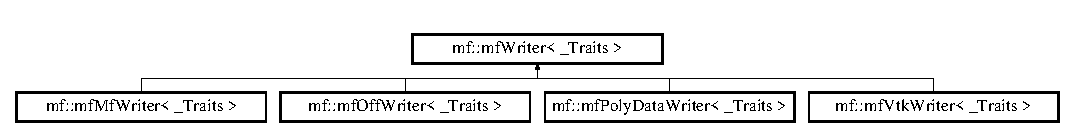
\includegraphics[height=1.407035cm]{classmf_1_1mfWriter}
\end{center}
\end{figure}
\subsection*{Public Types}
\begin{DoxyCompactItemize}
\item 
\hypertarget{classmf_1_1mfWriter_ab2e5e3009b068b86819bdb50a284809b}{
typedef \_\-Traits::sMesh {\bfseries sMesh}}
\label{classmf_1_1mfWriter_ab2e5e3009b068b86819bdb50a284809b}

\end{DoxyCompactItemize}
\subsection*{Public Member Functions}
\begin{DoxyCompactItemize}
\item 
\hyperlink{classmf_1_1mfWriter_a5c3d89035c391fcdb02e72efd5f6fb36}{mfWriter} ()
\item 
virtual \hyperlink{classmf_1_1mfWriter_acee9f2b54a145e68d165ab9fdb110865}{$\sim$mfWriter} ()
\item 
virtual bool \hyperlink{classmf_1_1mfWriter_a85d6c59bdb8fec69222e4157c299256c}{write} (sMesh $\ast$malha, const char $\ast$filename)=0
\begin{DoxyCompactList}\small\item\em Executa a escrita de um arquivo (salva uma malha) \item\end{DoxyCompactList}\end{DoxyCompactItemize}


\subsection{Detailed Description}
\subsubsection*{template$<$class \_\-Traits$>$ class mf::mfWriter$<$ \_\-Traits $>$}

Modelo dos escritores de arquivos. Esta classe eh abstrata, devendo servir apenas de molde para novas implementacoes de escritores de arquivos. 

\subsection{Constructor \& Destructor Documentation}
\hypertarget{classmf_1_1mfWriter_a5c3d89035c391fcdb02e72efd5f6fb36}{
\index{mf::mfWriter@{mf::mfWriter}!mfWriter@{mfWriter}}
\index{mfWriter@{mfWriter}!mf::mfWriter@{mf::mfWriter}}
\subsubsection[{mfWriter}]{\setlength{\rightskip}{0pt plus 5cm}template$<$class \_\-Traits $>$ {\bf mf::mfWriter}$<$ \_\-Traits $>$::{\bf mfWriter} (
\begin{DoxyParamCaption}
{}
\end{DoxyParamCaption}
)}}
\label{classmf_1_1mfWriter_a5c3d89035c391fcdb02e72efd5f6fb36}
Construtor \hypertarget{classmf_1_1mfWriter_acee9f2b54a145e68d165ab9fdb110865}{
\index{mf::mfWriter@{mf::mfWriter}!$\sim$mfWriter@{$\sim$mfWriter}}
\index{$\sim$mfWriter@{$\sim$mfWriter}!mf::mfWriter@{mf::mfWriter}}
\subsubsection[{$\sim$mfWriter}]{\setlength{\rightskip}{0pt plus 5cm}template$<$class \_\-Traits $>$ {\bf mf::mfWriter}$<$ \_\-Traits $>$::$\sim${\bf mfWriter} (
\begin{DoxyParamCaption}
{}
\end{DoxyParamCaption}
)\hspace{0.3cm}{\ttfamily  \mbox{[}virtual\mbox{]}}}}
\label{classmf_1_1mfWriter_acee9f2b54a145e68d165ab9fdb110865}
Destrutor 

\subsection{Member Function Documentation}
\hypertarget{classmf_1_1mfWriter_a85d6c59bdb8fec69222e4157c299256c}{
\index{mf::mfWriter@{mf::mfWriter}!write@{write}}
\index{write@{write}!mf::mfWriter@{mf::mfWriter}}
\subsubsection[{write}]{\setlength{\rightskip}{0pt plus 5cm}template$<$class \_\-Traits $>$ virtual bool {\bf mf::mfWriter}$<$ \_\-Traits $>$::write (
\begin{DoxyParamCaption}
\item[{sMesh $\ast$}]{malha, }
\item[{const char $\ast$}]{filename}
\end{DoxyParamCaption}
)\hspace{0.3cm}{\ttfamily  \mbox{[}pure virtual\mbox{]}}}}
\label{classmf_1_1mfWriter_a85d6c59bdb8fec69222e4157c299256c}


Executa a escrita de um arquivo (salva uma malha) 

Paraetros de entrada: malha : endereco de memoria da malha a ser salva. filename : nome do arquivo da malha. (destino) 

Implemented in \hyperlink{classmf_1_1mfMfWriter_a2fc75ae58c2e75f24924c812aec7bc8a}{mf::mfMfWriter$<$ \_\-Traits $>$}, \hyperlink{classmf_1_1mfOffWriter_ad3fe52bf8870c31c1b9f71431a56af8a}{mf::mfOffWriter$<$ \_\-Traits $>$}, \hyperlink{classmf_1_1mfPolyDataWriter_a5621f62f1a2811fa1b24da447cf3c5ea}{mf::mfPolyDataWriter$<$ \_\-Traits $>$}, and \hyperlink{classmf_1_1mfVtkWriter_a5385afe137ace0a1c5dafed8e74c4c35}{mf::mfVtkWriter$<$ \_\-Traits $>$}.



The documentation for this class was generated from the following file:\begin{DoxyCompactItemize}
\item 
mfWriter.h\end{DoxyCompactItemize}

\hypertarget{classmf_1_1mfWrlReader}{
\section{mf::mfWrlReader$<$ \_\-Traits $>$ Class Template Reference}
\label{classmf_1_1mfWrlReader}\index{mf::mfWrlReader@{mf::mfWrlReader}}
}
Inheritance diagram for mf::mfWrlReader$<$ \_\-Traits $>$:\begin{figure}[H]
\begin{center}
\leavevmode
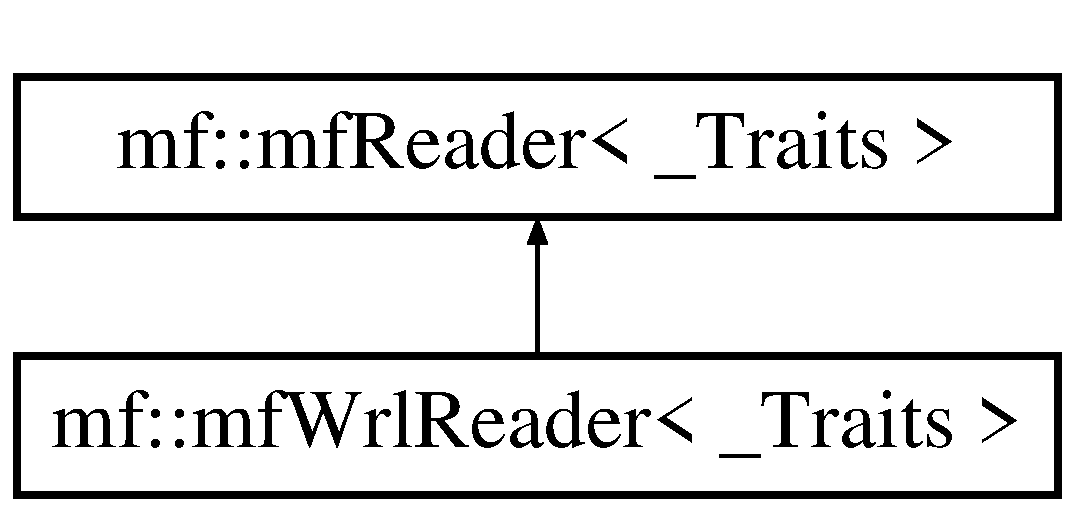
\includegraphics[height=2.000000cm]{classmf_1_1mfWrlReader}
\end{center}
\end{figure}
\subsection*{Public Types}
\begin{DoxyCompactItemize}
\item 
typedef \_\-Traits::space \hyperlink{classmf_1_1mfWrlReader_a1444633a52ae33327e44cab3b29a2547}{space}
\item 
typedef \_\-Traits::ids \hyperlink{classmf_1_1mfWrlReader_a218ccc566be4401a60f0b321effaae8c}{ids}
\item 
typedef \_\-Traits::sVertex \hyperlink{classmf_1_1mfWrlReader_a07a838e7ca326205d3f103aadcfc47a0}{sVertex}
\item 
typedef \_\-Traits::sCell \hyperlink{classmf_1_1mfWrlReader_a166fbf92ac3c8aad7eb1d8acf7f7541c}{sCell}
\item 
typedef \_\-Traits::sMesh \hyperlink{classmf_1_1mfWrlReader_a00a23984c72a850fbc105870596d6d78}{sMesh}
\end{DoxyCompactItemize}
\subsection*{Public Member Functions}
\begin{DoxyCompactItemize}
\item 
\hyperlink{classmf_1_1mfWrlReader_ac2a051b741b46ce2a41d2214a577e6b9}{mfWrlReader} ()
\item 
\hyperlink{classmf_1_1mfWrlReader_abb6561454375e4c8eb4d5f8ebb7e387b}{$\sim$mfWrlReader} ()
\item 
virtual bool \hyperlink{classmf_1_1mfWrlReader_a1d4c505e8e62204674aba4a36d47751e}{read} (\hyperlink{classmf_1_1mfWrlReader_a00a23984c72a850fbc105870596d6d78}{sMesh} $\ast$malha, const char $\ast$filename)
\begin{DoxyCompactList}\small\item\em Executa a leitura de um arquivo. \item\end{DoxyCompactList}\item 
\hypertarget{classmf_1_1mfWrlReader_a1962f16e07139e934a6b7c0dc6efd8a0}{
virtual bool {\bfseries read} (\hyperlink{classmf_1_1mfWrlReader_a00a23984c72a850fbc105870596d6d78}{sMesh} $\ast$malha, const char $\ast$filename, int cellDimension)}
\label{classmf_1_1mfWrlReader_a1962f16e07139e934a6b7c0dc6efd8a0}

\end{DoxyCompactItemize}
\subsubsection*{template$<$class \_\-Traits$>$ class mf::mfWrlReader$<$ \_\-Traits $>$}



\subsection{Member Typedef Documentation}
\hypertarget{classmf_1_1mfWrlReader_a218ccc566be4401a60f0b321effaae8c}{
\index{mf::mfWrlReader@{mf::mfWrlReader}!ids@{ids}}
\index{ids@{ids}!mf::mfWrlReader@{mf::mfWrlReader}}
\subsubsection[{ids}]{\setlength{\rightskip}{0pt plus 5cm}template$<$class \_\-Traits $>$ typedef \_\-Traits::ids {\bf mf::mfWrlReader}$<$ \_\-Traits $>$::{\bf ids}}}
\label{classmf_1_1mfWrlReader_a218ccc566be4401a60f0b321effaae8c}
Id typename definition \hypertarget{classmf_1_1mfWrlReader_a166fbf92ac3c8aad7eb1d8acf7f7541c}{
\index{mf::mfWrlReader@{mf::mfWrlReader}!sCell@{sCell}}
\index{sCell@{sCell}!mf::mfWrlReader@{mf::mfWrlReader}}
\subsubsection[{sCell}]{\setlength{\rightskip}{0pt plus 5cm}template$<$class \_\-Traits $>$ typedef \_\-Traits::sCell {\bf mf::mfWrlReader}$<$ \_\-Traits $>$::{\bf sCell}}}
\label{classmf_1_1mfWrlReader_a166fbf92ac3c8aad7eb1d8acf7f7541c}
Cell typename definition \hypertarget{classmf_1_1mfWrlReader_a00a23984c72a850fbc105870596d6d78}{
\index{mf::mfWrlReader@{mf::mfWrlReader}!sMesh@{sMesh}}
\index{sMesh@{sMesh}!mf::mfWrlReader@{mf::mfWrlReader}}
\subsubsection[{sMesh}]{\setlength{\rightskip}{0pt plus 5cm}template$<$class \_\-Traits $>$ typedef \_\-Traits::sMesh {\bf mf::mfWrlReader}$<$ \_\-Traits $>$::{\bf sMesh}}}
\label{classmf_1_1mfWrlReader_a00a23984c72a850fbc105870596d6d78}
Mesh typename definition 

Reimplemented from \hyperlink{classmf_1_1mfReader}{mf::mfReader$<$ \_\-Traits $>$}.

\hypertarget{classmf_1_1mfWrlReader_a1444633a52ae33327e44cab3b29a2547}{
\index{mf::mfWrlReader@{mf::mfWrlReader}!space@{space}}
\index{space@{space}!mf::mfWrlReader@{mf::mfWrlReader}}
\subsubsection[{space}]{\setlength{\rightskip}{0pt plus 5cm}template$<$class \_\-Traits $>$ typedef \_\-Traits::space {\bf mf::mfWrlReader}$<$ \_\-Traits $>$::{\bf space}}}
\label{classmf_1_1mfWrlReader_a1444633a52ae33327e44cab3b29a2547}
Space typename definition \hypertarget{classmf_1_1mfWrlReader_a07a838e7ca326205d3f103aadcfc47a0}{
\index{mf::mfWrlReader@{mf::mfWrlReader}!sVertex@{sVertex}}
\index{sVertex@{sVertex}!mf::mfWrlReader@{mf::mfWrlReader}}
\subsubsection[{sVertex}]{\setlength{\rightskip}{0pt plus 5cm}template$<$class \_\-Traits $>$ typedef \_\-Traits::sVertex {\bf mf::mfWrlReader}$<$ \_\-Traits $>$::{\bf sVertex}}}
\label{classmf_1_1mfWrlReader_a07a838e7ca326205d3f103aadcfc47a0}
Vertex typename definition 

\subsection{Constructor \& Destructor Documentation}
\hypertarget{classmf_1_1mfWrlReader_ac2a051b741b46ce2a41d2214a577e6b9}{
\index{mf::mfWrlReader@{mf::mfWrlReader}!mfWrlReader@{mfWrlReader}}
\index{mfWrlReader@{mfWrlReader}!mf::mfWrlReader@{mf::mfWrlReader}}
\subsubsection[{mfWrlReader}]{\setlength{\rightskip}{0pt plus 5cm}template$<$class \_\-Traits $>$ {\bf mf::mfWrlReader}$<$ \_\-Traits $>$::{\bf mfWrlReader} (
\begin{DoxyParamCaption}
{}
\end{DoxyParamCaption}
)}}
\label{classmf_1_1mfWrlReader_ac2a051b741b46ce2a41d2214a577e6b9}
Constructor \hypertarget{classmf_1_1mfWrlReader_abb6561454375e4c8eb4d5f8ebb7e387b}{
\index{mf::mfWrlReader@{mf::mfWrlReader}!$\sim$mfWrlReader@{$\sim$mfWrlReader}}
\index{$\sim$mfWrlReader@{$\sim$mfWrlReader}!mf::mfWrlReader@{mf::mfWrlReader}}
\subsubsection[{$\sim$mfWrlReader}]{\setlength{\rightskip}{0pt plus 5cm}template$<$class \_\-Traits $>$ {\bf mf::mfWrlReader}$<$ \_\-Traits $>$::$\sim${\bf mfWrlReader} (
\begin{DoxyParamCaption}
{}
\end{DoxyParamCaption}
)}}
\label{classmf_1_1mfWrlReader_abb6561454375e4c8eb4d5f8ebb7e387b}
Destructor 

\subsection{Member Function Documentation}
\hypertarget{classmf_1_1mfWrlReader_a1d4c505e8e62204674aba4a36d47751e}{
\index{mf::mfWrlReader@{mf::mfWrlReader}!read@{read}}
\index{read@{read}!mf::mfWrlReader@{mf::mfWrlReader}}
\subsubsection[{read}]{\setlength{\rightskip}{0pt plus 5cm}template$<$class \_\-Traits $>$ bool {\bf mf::mfWrlReader}$<$ \_\-Traits $>$::read (
\begin{DoxyParamCaption}
\item[{{\bf sMesh} $\ast$}]{malha, }
\item[{const char $\ast$}]{filename}
\end{DoxyParamCaption}
)\hspace{0.3cm}{\ttfamily  \mbox{[}virtual\mbox{]}}}}
\label{classmf_1_1mfWrlReader_a1d4c505e8e62204674aba4a36d47751e}


Executa a leitura de um arquivo. 

Paraetros de entrada: malha : endereco de memoria de destino da malha a ser carregada. Ja deve estar alocado. filename : nome do arquivo da malha. 

Implements \hyperlink{classmf_1_1mfReader_a0e0c3224a06b06a8fb82be4f0f4a2e00}{mf::mfReader$<$ \_\-Traits $>$}.



The documentation for this class was generated from the following file:\begin{DoxyCompactItemize}
\item 
mfWrlReader.h\end{DoxyCompactItemize}

\hypertarget{classmf_1_1mfXmlParser}{
\section{mf::mfXmlParser Class Reference}
\label{classmf_1_1mfXmlParser}\index{mf::mfXmlParser@{mf::mfXmlParser}}
}
\subsection*{Public Member Functions}
\begin{DoxyCompactItemize}
\item 
\hyperlink{classmf_1_1mfXmlParser_ad4d1a1064182d64ad3e116daceecb018}{mfXmlParser} ()
\item 
\hyperlink{classmf_1_1mfXmlParser_a3f6584db78e276c1bd66825d42163098}{$\sim$mfXmlParser} ()
\item 
\hypertarget{classmf_1_1mfXmlParser_a7a76341346a3669a8a1f706dcf7613e7}{
bool {\bfseries read} (const char $\ast$arquivo)}
\label{classmf_1_1mfXmlParser_a7a76341346a3669a8a1f706dcf7613e7}

\item 
\hypertarget{classmf_1_1mfXmlParser_a48bf5f394dbb9261d84e69b70316044b}{
char $\ast$ {\bfseries getHost} ()}
\label{classmf_1_1mfXmlParser_a48bf5f394dbb9261d84e69b70316044b}

\item 
\hypertarget{classmf_1_1mfXmlParser_ac73b0f2f4ef196d1ed067916d37718b2}{
char $\ast$ {\bfseries getPort} ()}
\label{classmf_1_1mfXmlParser_ac73b0f2f4ef196d1ed067916d37718b2}

\item 
\hypertarget{classmf_1_1mfXmlParser_aa89c926cb5e642e66a602c727cb9d1fa}{
char $\ast$ {\bfseries getUser} ()}
\label{classmf_1_1mfXmlParser_aa89c926cb5e642e66a602c727cb9d1fa}

\item 
\hypertarget{classmf_1_1mfXmlParser_a2ac7f2d957209d909f0c8335f979c1b4}{
char $\ast$ {\bfseries getPassword} ()}
\label{classmf_1_1mfXmlParser_a2ac7f2d957209d909f0c8335f979c1b4}

\item 
\hypertarget{classmf_1_1mfXmlParser_a808bcb47487139644fa68e330a1ccfe0}{
char $\ast$ {\bfseries getDataBase} ()}
\label{classmf_1_1mfXmlParser_a808bcb47487139644fa68e330a1ccfe0}

\item 
\hypertarget{classmf_1_1mfXmlParser_ac3c107b483e29c82c66fe959aa1adf59}{
char $\ast$ {\bfseries getVerticesTable} ()}
\label{classmf_1_1mfXmlParser_ac3c107b483e29c82c66fe959aa1adf59}

\item 
\hypertarget{classmf_1_1mfXmlParser_aaa25bd925e9fb92c0d2a4afdc80ed046}{
char $\ast$ {\bfseries getCellsTable} ()}
\label{classmf_1_1mfXmlParser_aaa25bd925e9fb92c0d2a4afdc80ed046}

\item 
\hypertarget{classmf_1_1mfXmlParser_a273076f391bcc7459179f7fbbdd0bc0d}{
char $\ast$ {\bfseries getVerticesIdField} ()}
\label{classmf_1_1mfXmlParser_a273076f391bcc7459179f7fbbdd0bc0d}

\item 
\hypertarget{classmf_1_1mfXmlParser_a433500baf91d1491d7a04974f155e56a}{
int {\bfseries getVerticesDimension} ()}
\label{classmf_1_1mfXmlParser_a433500baf91d1491d7a04974f155e56a}

\item 
\hypertarget{classmf_1_1mfXmlParser_a442fa61be035b5a792ec4c91a256977c}{
char $\ast$ {\bfseries getVerticesField} (int dim)}
\label{classmf_1_1mfXmlParser_a442fa61be035b5a792ec4c91a256977c}

\item 
\hypertarget{classmf_1_1mfXmlParser_a958d029921ec2a95dadd87f27e921608}{
char $\ast$ {\bfseries getCellsIdField} ()}
\label{classmf_1_1mfXmlParser_a958d029921ec2a95dadd87f27e921608}

\item 
\hypertarget{classmf_1_1mfXmlParser_a0c4412e03aa03b209dd8aa9ac8e2c2d3}{
int {\bfseries getCellsDimension} ()}
\label{classmf_1_1mfXmlParser_a0c4412e03aa03b209dd8aa9ac8e2c2d3}

\item 
\hypertarget{classmf_1_1mfXmlParser_af0d25974b03b6a8989eaca6ca1636e66}{
char $\ast$ {\bfseries getCellsField} (int dim)}
\label{classmf_1_1mfXmlParser_af0d25974b03b6a8989eaca6ca1636e66}

\end{DoxyCompactItemize}


\subsection{Constructor \& Destructor Documentation}
\hypertarget{classmf_1_1mfXmlParser_ad4d1a1064182d64ad3e116daceecb018}{
\index{mf::mfXmlParser@{mf::mfXmlParser}!mfXmlParser@{mfXmlParser}}
\index{mfXmlParser@{mfXmlParser}!mf::mfXmlParser@{mf::mfXmlParser}}
\subsubsection[{mfXmlParser}]{\setlength{\rightskip}{0pt plus 5cm}mf::mfXmlParser::mfXmlParser (
\begin{DoxyParamCaption}
{}
\end{DoxyParamCaption}
)\hspace{0.3cm}{\ttfamily  \mbox{[}inline\mbox{]}}}}
\label{classmf_1_1mfXmlParser_ad4d1a1064182d64ad3e116daceecb018}
Constructor \hypertarget{classmf_1_1mfXmlParser_a3f6584db78e276c1bd66825d42163098}{
\index{mf::mfXmlParser@{mf::mfXmlParser}!$\sim$mfXmlParser@{$\sim$mfXmlParser}}
\index{$\sim$mfXmlParser@{$\sim$mfXmlParser}!mf::mfXmlParser@{mf::mfXmlParser}}
\subsubsection[{$\sim$mfXmlParser}]{\setlength{\rightskip}{0pt plus 5cm}mf::mfXmlParser::$\sim$mfXmlParser (
\begin{DoxyParamCaption}
{}
\end{DoxyParamCaption}
)\hspace{0.3cm}{\ttfamily  \mbox{[}inline\mbox{]}}}}
\label{classmf_1_1mfXmlParser_a3f6584db78e276c1bd66825d42163098}
Destructor 

The documentation for this class was generated from the following file:\begin{DoxyCompactItemize}
\item 
mfXmlParser.h\end{DoxyCompactItemize}

\hypertarget{classmf_1_1myTsReader}{
\section{mf::myTsReader$<$ \_\-Traits $>$ Class Template Reference}
\label{classmf_1_1myTsReader}\index{mf::myTsReader@{mf::myTsReader}}
}
Inheritance diagram for mf::myTsReader$<$ \_\-Traits $>$:\begin{figure}[H]
\begin{center}
\leavevmode
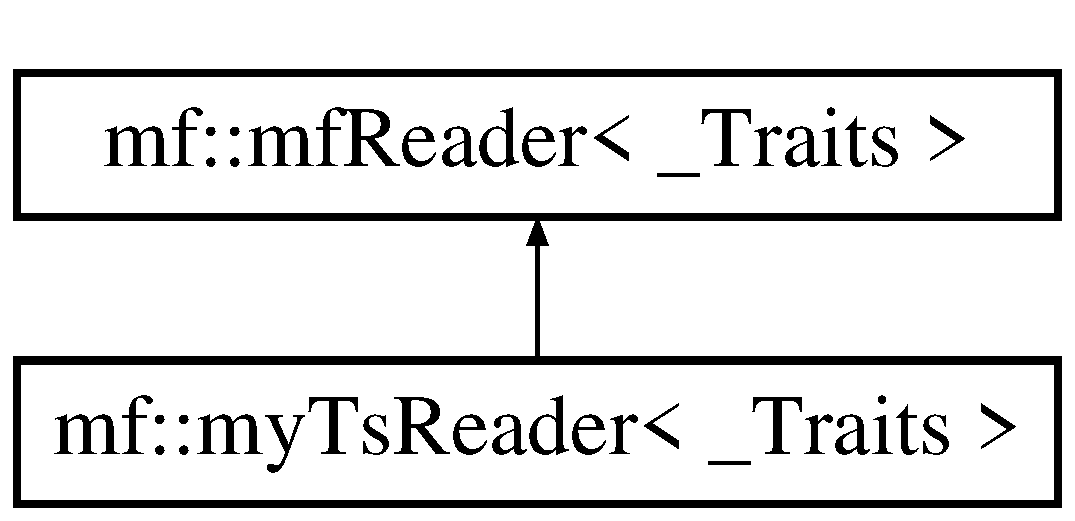
\includegraphics[height=2.000000cm]{classmf_1_1myTsReader}
\end{center}
\end{figure}
\subsection*{Public Types}
\begin{DoxyCompactItemize}
\item 
typedef \_\-Traits::space \hyperlink{classmf_1_1myTsReader_a093186d16379743990dcec3f7eb78f20}{space}
\item 
typedef \_\-Traits::ids \hyperlink{classmf_1_1myTsReader_ad3ffe55514e0229db84f085cc1d88c99}{ids}
\item 
typedef \_\-Traits::sVertex \hyperlink{classmf_1_1myTsReader_a4844880ee2a7a3656545dce76bbcaaba}{sVertex}
\item 
typedef \_\-Traits::sCell \hyperlink{classmf_1_1myTsReader_a38e884b502c798830b1598e6f56f97bc}{sCell}
\item 
typedef \_\-Traits::sMesh \hyperlink{classmf_1_1myTsReader_a2b17f65a22359c58f4cbf59b289a3284}{sMesh}
\end{DoxyCompactItemize}
\subsection*{Public Member Functions}
\begin{DoxyCompactItemize}
\item 
\hyperlink{classmf_1_1myTsReader_ab0a76a68ceb12ee2e90f913147ab273e}{myTsReader} ()
\item 
\hyperlink{classmf_1_1myTsReader_a03df726db3f0ab6b7ff45e58772bbfaa}{$\sim$myTsReader} ()
\item 
virtual bool \hyperlink{classmf_1_1myTsReader_a84fa0feda9979c77cfb609f3310fd31e}{read} (\hyperlink{classmf_1_1myTsReader_a2b17f65a22359c58f4cbf59b289a3284}{sMesh} $\ast$malha, const char $\ast$filename)
\begin{DoxyCompactList}\small\item\em Executa a leitura de um arquivo. \item\end{DoxyCompactList}\end{DoxyCompactItemize}
\subsubsection*{template$<$class \_\-Traits$>$ class mf::myTsReader$<$ \_\-Traits $>$}



\subsection{Member Typedef Documentation}
\hypertarget{classmf_1_1myTsReader_ad3ffe55514e0229db84f085cc1d88c99}{
\index{mf::myTsReader@{mf::myTsReader}!ids@{ids}}
\index{ids@{ids}!mf::myTsReader@{mf::myTsReader}}
\subsubsection[{ids}]{\setlength{\rightskip}{0pt plus 5cm}template$<$class \_\-Traits $>$ typedef \_\-Traits::ids {\bf mf::myTsReader}$<$ \_\-Traits $>$::{\bf ids}}}
\label{classmf_1_1myTsReader_ad3ffe55514e0229db84f085cc1d88c99}
Id typename definition \hypertarget{classmf_1_1myTsReader_a38e884b502c798830b1598e6f56f97bc}{
\index{mf::myTsReader@{mf::myTsReader}!sCell@{sCell}}
\index{sCell@{sCell}!mf::myTsReader@{mf::myTsReader}}
\subsubsection[{sCell}]{\setlength{\rightskip}{0pt plus 5cm}template$<$class \_\-Traits $>$ typedef \_\-Traits::sCell {\bf mf::myTsReader}$<$ \_\-Traits $>$::{\bf sCell}}}
\label{classmf_1_1myTsReader_a38e884b502c798830b1598e6f56f97bc}
Cell typename definition \hypertarget{classmf_1_1myTsReader_a2b17f65a22359c58f4cbf59b289a3284}{
\index{mf::myTsReader@{mf::myTsReader}!sMesh@{sMesh}}
\index{sMesh@{sMesh}!mf::myTsReader@{mf::myTsReader}}
\subsubsection[{sMesh}]{\setlength{\rightskip}{0pt plus 5cm}template$<$class \_\-Traits $>$ typedef \_\-Traits::sMesh {\bf mf::myTsReader}$<$ \_\-Traits $>$::{\bf sMesh}}}
\label{classmf_1_1myTsReader_a2b17f65a22359c58f4cbf59b289a3284}
Mesh typename definition 

Reimplemented from \hyperlink{classmf_1_1mfReader}{mf::mfReader$<$ \_\-Traits $>$}.

\hypertarget{classmf_1_1myTsReader_a093186d16379743990dcec3f7eb78f20}{
\index{mf::myTsReader@{mf::myTsReader}!space@{space}}
\index{space@{space}!mf::myTsReader@{mf::myTsReader}}
\subsubsection[{space}]{\setlength{\rightskip}{0pt plus 5cm}template$<$class \_\-Traits $>$ typedef \_\-Traits::space {\bf mf::myTsReader}$<$ \_\-Traits $>$::{\bf space}}}
\label{classmf_1_1myTsReader_a093186d16379743990dcec3f7eb78f20}
Space typename definition \hypertarget{classmf_1_1myTsReader_a4844880ee2a7a3656545dce76bbcaaba}{
\index{mf::myTsReader@{mf::myTsReader}!sVertex@{sVertex}}
\index{sVertex@{sVertex}!mf::myTsReader@{mf::myTsReader}}
\subsubsection[{sVertex}]{\setlength{\rightskip}{0pt plus 5cm}template$<$class \_\-Traits $>$ typedef \_\-Traits::sVertex {\bf mf::myTsReader}$<$ \_\-Traits $>$::{\bf sVertex}}}
\label{classmf_1_1myTsReader_a4844880ee2a7a3656545dce76bbcaaba}
Vertex typename definition 

\subsection{Constructor \& Destructor Documentation}
\hypertarget{classmf_1_1myTsReader_ab0a76a68ceb12ee2e90f913147ab273e}{
\index{mf::myTsReader@{mf::myTsReader}!myTsReader@{myTsReader}}
\index{myTsReader@{myTsReader}!mf::myTsReader@{mf::myTsReader}}
\subsubsection[{myTsReader}]{\setlength{\rightskip}{0pt plus 5cm}template$<$class \_\-Traits $>$ {\bf mf::myTsReader}$<$ \_\-Traits $>$::{\bf myTsReader} (
\begin{DoxyParamCaption}
{}
\end{DoxyParamCaption}
)}}
\label{classmf_1_1myTsReader_ab0a76a68ceb12ee2e90f913147ab273e}
Constructor \hypertarget{classmf_1_1myTsReader_a03df726db3f0ab6b7ff45e58772bbfaa}{
\index{mf::myTsReader@{mf::myTsReader}!$\sim$myTsReader@{$\sim$myTsReader}}
\index{$\sim$myTsReader@{$\sim$myTsReader}!mf::myTsReader@{mf::myTsReader}}
\subsubsection[{$\sim$myTsReader}]{\setlength{\rightskip}{0pt plus 5cm}template$<$class \_\-Traits $>$ {\bf mf::myTsReader}$<$ \_\-Traits $>$::$\sim${\bf myTsReader} (
\begin{DoxyParamCaption}
{}
\end{DoxyParamCaption}
)}}
\label{classmf_1_1myTsReader_a03df726db3f0ab6b7ff45e58772bbfaa}
Destructor 

\subsection{Member Function Documentation}
\hypertarget{classmf_1_1myTsReader_a84fa0feda9979c77cfb609f3310fd31e}{
\index{mf::myTsReader@{mf::myTsReader}!read@{read}}
\index{read@{read}!mf::myTsReader@{mf::myTsReader}}
\subsubsection[{read}]{\setlength{\rightskip}{0pt plus 5cm}template$<$class \_\-Traits $>$ bool {\bf mf::myTsReader}$<$ \_\-Traits $>$::read (
\begin{DoxyParamCaption}
\item[{{\bf sMesh} $\ast$}]{malha, }
\item[{const char $\ast$}]{filename}
\end{DoxyParamCaption}
)\hspace{0.3cm}{\ttfamily  \mbox{[}virtual\mbox{]}}}}
\label{classmf_1_1myTsReader_a84fa0feda9979c77cfb609f3310fd31e}


Executa a leitura de um arquivo. 

Paraetros de entrada: malha : endereco de memoria de destino da malha a ser carregada. Ja deve estar alocado. filename : nome do arquivo da malha. 

Implements \hyperlink{classmf_1_1mfReader_a0e0c3224a06b06a8fb82be4f0f4a2e00}{mf::mfReader$<$ \_\-Traits $>$}.



The documentation for this class was generated from the following file:\begin{DoxyCompactItemize}
\item 
myTsReader.h\end{DoxyCompactItemize}

\hypertarget{classmf_1_1mfDelaunay2D_1_1sObject}{
\section{mf::mfDelaunay2D$<$ \_\-Traits $>$::sObject Class Reference}
\label{classmf_1_1mfDelaunay2D_1_1sObject}\index{mf::mfDelaunay2D::sObject@{mf::mfDelaunay2D::sObject}}
}
\subsection*{Public Member Functions}
\begin{DoxyCompactItemize}
\item 
\hypertarget{classmf_1_1mfDelaunay2D_1_1sObject_ab7f3c45c96326b694c3aca4c8b86328f}{
{\bfseries sObject} (\hyperlink{classmf_1_1mfDelaunay2D_a6459b2d8aa82aedabc7be094a80fac5f}{sVertex} $\ast$\_\-v, \hyperlink{classmf_1_1mfDelaunay2D_af821015a498654435308272878e686f2}{ids} \_\-id)}
\label{classmf_1_1mfDelaunay2D_1_1sObject_ab7f3c45c96326b694c3aca4c8b86328f}

\end{DoxyCompactItemize}
\subsection*{Public Attributes}
\begin{DoxyCompactItemize}
\item 
\hypertarget{classmf_1_1mfDelaunay2D_1_1sObject_a38973d89f26ded099e59325e31808cd2}{
\hyperlink{classmf_1_1mfDelaunay2D_a6459b2d8aa82aedabc7be094a80fac5f}{sVertex} $\ast$ {\bfseries v}}
\label{classmf_1_1mfDelaunay2D_1_1sObject_a38973d89f26ded099e59325e31808cd2}

\item 
\hypertarget{classmf_1_1mfDelaunay2D_1_1sObject_abbcf2c4f0f09f9d39010b2dbd796bfc0}{
\hyperlink{classmf_1_1mfDelaunay2D_af821015a498654435308272878e686f2}{ids} {\bfseries id}}
\label{classmf_1_1mfDelaunay2D_1_1sObject_abbcf2c4f0f09f9d39010b2dbd796bfc0}

\end{DoxyCompactItemize}
\subsubsection*{template$<$class \_\-Traits$>$ class mf::mfDelaunay2D$<$ \_\-Traits $>$::sObject}



The documentation for this class was generated from the following file:\begin{DoxyCompactItemize}
\item 
mfDelaunay2D.h\end{DoxyCompactItemize}

\hypertarget{classmf_1_1mfDelaunay2D_1_1sObjectCompare}{
\section{mf::mfDelaunay2D$<$ \_\-Traits $>$::sObjectCompare Class Reference}
\label{classmf_1_1mfDelaunay2D_1_1sObjectCompare}\index{mf::mfDelaunay2D::sObjectCompare@{mf::mfDelaunay2D::sObjectCompare}}
}
\subsection*{Public Member Functions}
\begin{DoxyCompactItemize}
\item 
\hypertarget{classmf_1_1mfDelaunay2D_1_1sObjectCompare_ae04c997519cf31450226f0bcc8f41359}{
bool {\bfseries greater} (\hyperlink{classmf_1_1mfDelaunay2D_1_1sObject}{sObject} $\ast$v1, \hyperlink{classmf_1_1mfDelaunay2D_1_1sObject}{sObject} $\ast$v2, int dim)}
\label{classmf_1_1mfDelaunay2D_1_1sObjectCompare_ae04c997519cf31450226f0bcc8f41359}

\end{DoxyCompactItemize}
\subsubsection*{template$<$class \_\-Traits$>$ class mf::mfDelaunay2D$<$ \_\-Traits $>$::sObjectCompare}



The documentation for this class was generated from the following file:\begin{DoxyCompactItemize}
\item 
mfDelaunay2D.h\end{DoxyCompactItemize}

\chapter{File Documentation}
\hypertarget{mfBase_8h}{
\section{mfBase.h File Reference}
\label{mfBase_8h}\index{mfBase.h@{mfBase.h}}
}


Base Class Base Class for all elements of mesh.  


{\ttfamily \#include \char`\"{}mfMacros.h\char`\"{}}\par
\subsection*{Classes}
\begin{DoxyCompactItemize}
\item 
class \hyperlink{classmf_1_1mfBase}{mf::mfBase$<$ \_\-Traits $>$}
\end{DoxyCompactItemize}
\subsection*{Namespaces}
\begin{DoxyCompactItemize}
\item 
namespace \hyperlink{namespacemf}{mf}
\end{DoxyCompactItemize}
\subsection*{Defines}
\begin{DoxyCompactItemize}
\item 
\hypertarget{mfBase_8h_aa88ff7d611e26703bc645eb3acd225f7}{
\#define {\bfseries IDS}~typename mfBase$<$\_\-Traits$>$::ids}
\label{mfBase_8h_aa88ff7d611e26703bc645eb3acd225f7}

\end{DoxyCompactItemize}


\subsection{Detailed Description}
Base Class Base Class for all elements of mesh. \_\-Traits must have ids typename

\begin{DoxyAuthor}{Author}
Mario Lizier 
\end{DoxyAuthor}
\begin{DoxyVersion}{Version}
1.0 
\end{DoxyVersion}
\begin{DoxyDate}{Date}
2007, july 
\end{DoxyDate}

\hypertarget{mfCell_8h}{
\section{mfCell.h File Reference}
\label{mfCell_8h}\index{mfCell.h@{mfCell.h}}
}


Base class of the cell.  


{\ttfamily \#include \char`\"{}mfMacros.h\char`\"{}}\par
{\ttfamily \#include \char`\"{}mfBase.h\char`\"{}}\par
\subsection*{Classes}
\begin{DoxyCompactItemize}
\item 
class \hyperlink{classmf_1_1mfCell}{mf::mfCell$<$ size, \_\-Traits $>$}
\end{DoxyCompactItemize}
\subsection*{Namespaces}
\begin{DoxyCompactItemize}
\item 
namespace \hyperlink{namespacemf}{mf}
\end{DoxyCompactItemize}
\subsection*{Defines}
\begin{DoxyCompactItemize}
\item 
\hypertarget{mfCell_8h_aa88ff7d611e26703bc645eb3acd225f7}{
\#define {\bfseries IDS}~typename mfCell$<$size,\_\-Traits$>$::ids}
\label{mfCell_8h_aa88ff7d611e26703bc645eb3acd225f7}

\end{DoxyCompactItemize}


\subsection{Detailed Description}
Base class of the cell. Cell types are: 2D -\/ triangles, quadrilaterals and hybrid surface 3D -\/ tetrahedra, hexahedra, prism, piramids and hybrid volumetric

\_\-Traits must have typenames: ids

\begin{DoxyAuthor}{Author}
Mario Lizier and Icaro da Cunha 
\end{DoxyAuthor}
\begin{DoxyVersion}{Version}
1.0 
\end{DoxyVersion}
\begin{DoxyDate}{Date}
2008, july 
\end{DoxyDate}

\hypertarget{mfCellsIterator_8h}{
\section{mfCellsIterator.h File Reference}
\label{mfCellsIterator_8h}\index{mfCellsIterator.h@{mfCellsIterator.h}}
}


Cell iterator class.  


{\ttfamily \#include \char`\"{}mfMacros.h\char`\"{}}\par
{\ttfamily \#include \char`\"{}mfMesh.h\char`\"{}}\par
{\ttfamily \#include \char`\"{}mfIterator.h\char`\"{}}\par
\subsection*{Classes}
\begin{DoxyCompactItemize}
\item 
class \hyperlink{classmf_1_1mfCellsIterator}{mf::mfCellsIterator$<$ \_\-Traits $>$}
\end{DoxyCompactItemize}
\subsection*{Namespaces}
\begin{DoxyCompactItemize}
\item 
namespace \hyperlink{namespacemf}{mf}
\end{DoxyCompactItemize}
\subsection*{Defines}
\begin{DoxyCompactItemize}
\item 
\hypertarget{mfCellsIterator_8h_a037e9cf6a1c91e1bc13ee32edb5058fb}{
\#define {\bfseries SCELL}~typename mfCellsIterator$<$\_\-Traits$>$::sCell}
\label{mfCellsIterator_8h_a037e9cf6a1c91e1bc13ee32edb5058fb}

\item 
\hypertarget{mfCellsIterator_8h_aa88ff7d611e26703bc645eb3acd225f7}{
\#define {\bfseries IDS}~typename mfCellsIterator$<$\_\-Traits$>$::ids}
\label{mfCellsIterator_8h_aa88ff7d611e26703bc645eb3acd225f7}

\end{DoxyCompactItemize}


\subsection{Detailed Description}
Cell iterator class. Iterator for the meshe's cell vector

\_\-Traits must have typenames: ids, sCell, sMesh

\begin{DoxyAuthor}{Author}
Mario Lizier 
\end{DoxyAuthor}
\begin{DoxyVersion}{Version}
1.0 
\end{DoxyVersion}
\begin{DoxyDate}{Date}
2007, july 
\end{DoxyDate}

\hypertarget{mfEdge_8h}{
\section{mfEdge.h File Reference}
\label{mfEdge_8h}\index{mfEdge.h@{mfEdge.h}}
}


Base class of the edge.  


{\ttfamily \#include \char`\"{}mfMacros.h\char`\"{}}\par
{\ttfamily \#include \char`\"{}mfBase.h\char`\"{}}\par
\subsection*{Classes}
\begin{DoxyCompactItemize}
\item 
class \hyperlink{classmf_1_1mfEdge}{mf::mfEdge$<$ \_\-Traits $>$}
\end{DoxyCompactItemize}
\subsection*{Namespaces}
\begin{DoxyCompactItemize}
\item 
namespace \hyperlink{namespacemf}{mf}
\end{DoxyCompactItemize}


\subsection{Detailed Description}
Base class of the edge. \begin{DoxyAuthor}{Author}
Icaro da Cunha 
\end{DoxyAuthor}
\begin{DoxyVersion}{Version}
1.0 
\end{DoxyVersion}
\begin{DoxyDate}{Date}
2008, july 
\end{DoxyDate}

\hypertarget{mfEdgesIterator_8h}{
\section{mfEdgesIterator.h File Reference}
\label{mfEdgesIterator_8h}\index{mfEdgesIterator.h@{mfEdgesIterator.h}}
}


Edge iterator class.  


{\ttfamily \#include \char`\"{}mfMacros.h\char`\"{}}\par
{\ttfamily \#include \char`\"{}mfMesh.h\char`\"{}}\par
{\ttfamily \#include \char`\"{}mfIterator.h\char`\"{}}\par
\subsection*{Classes}
\begin{DoxyCompactItemize}
\item 
class \hyperlink{classmf_1_1mfEdgesIterator}{mf::mfEdgesIterator$<$ \_\-Traits $>$}
\end{DoxyCompactItemize}
\subsection*{Namespaces}
\begin{DoxyCompactItemize}
\item 
namespace \hyperlink{namespacemf}{mf}
\end{DoxyCompactItemize}
\subsection*{Defines}
\begin{DoxyCompactItemize}
\item 
\hypertarget{mfEdgesIterator_8h_acb5cecc15e2452b8b1e880374e6ecab6}{
\#define {\bfseries SEDGE}~typename mfEdgesIterator$<$\_\-Traits$>$::sEdge}
\label{mfEdgesIterator_8h_acb5cecc15e2452b8b1e880374e6ecab6}

\item 
\hypertarget{mfEdgesIterator_8h_aa88ff7d611e26703bc645eb3acd225f7}{
\#define {\bfseries IDS}~typename mfEdgesIterator$<$\_\-Traits$>$::ids}
\label{mfEdgesIterator_8h_aa88ff7d611e26703bc645eb3acd225f7}

\end{DoxyCompactItemize}


\subsection{Detailed Description}
Edge iterator class. Iterator for the meshe's edge vector

\_\-Traits must have typenames: ids, sEdge, sMesh

\begin{DoxyAuthor}{Author}
Icaro da Cunha 
\end{DoxyAuthor}
\begin{DoxyVersion}{Version}
1.0 
\end{DoxyVersion}
\begin{DoxyDate}{Date}
2008, july 
\end{DoxyDate}

\hypertarget{mfFace_8h}{
\section{mfFace.h File Reference}
\label{mfFace_8h}\index{mfFace.h@{mfFace.h}}
}


Base class of the face.  


{\ttfamily \#include \char`\"{}mfMacros.h\char`\"{}}\par
{\ttfamily \#include \char`\"{}mfBase.h\char`\"{}}\par
\subsection*{Classes}
\begin{DoxyCompactItemize}
\item 
class \hyperlink{classmf_1_1mfFace}{mf::mfFace$<$ \_\-Traits $>$}
\end{DoxyCompactItemize}
\subsection*{Namespaces}
\begin{DoxyCompactItemize}
\item 
namespace \hyperlink{namespacemf}{mf}
\end{DoxyCompactItemize}


\subsection{Detailed Description}
Base class of the face. \begin{DoxyAuthor}{Author}
Icaro da Cunha 
\end{DoxyAuthor}
\begin{DoxyVersion}{Version}
1.0 
\end{DoxyVersion}
\begin{DoxyDate}{Date}
2008, july 
\end{DoxyDate}

\hypertarget{mfHexaCell_8h}{
\section{mfHexaCell.h File Reference}
\label{mfHexaCell_8h}\index{mfHexaCell.h@{mfHexaCell.h}}
}


Base class of the hexahedron cell.  


{\ttfamily \#include \char`\"{}mfMacros.h\char`\"{}}\par
{\ttfamily \#include \char`\"{}mfCell.h\char`\"{}}\par
\subsection*{Classes}
\begin{DoxyCompactItemize}
\item 
class \hyperlink{classmf_1_1mfHexaCell}{mf::mfHexaCell$<$ \_\-Traits $>$}
\end{DoxyCompactItemize}
\subsection*{Namespaces}
\begin{DoxyCompactItemize}
\item 
namespace \hyperlink{namespacemf}{mf}
\end{DoxyCompactItemize}
\subsection*{Defines}
\begin{DoxyCompactItemize}
\item 
\hypertarget{mfHexaCell_8h_aa88ff7d611e26703bc645eb3acd225f7}{
\#define {\bfseries IDS}~typename mfHexaCell$<$\_\-Traits$>$::ids}
\label{mfHexaCell_8h_aa88ff7d611e26703bc645eb3acd225f7}

\end{DoxyCompactItemize}


\subsection{Detailed Description}
Base class of the hexahedron cell. Hexahedron cell default format with vertex indices: 7-\/-\/-\/-\/-\/-\/-\/-\/-\/-\/6 /$|$ /$|$ / / $|$ / $|$ / $|$ 4-\/-\/-\/-\/-\/-\/-\/-\/-\/-\/5 $|$ $|$ $|$ $|$ $|$ $|$ 3-\/ -\/ -\/$|$-\/ -\/2 $|$ / $|$ / $|$ $|$ / $|$/ $|$/ 0-\/-\/-\/-\/-\/-\/-\/-\/-\/-\/1

\_\-Traits must have typenames: ids

\begin{DoxyAuthor}{Author}
Icaro da Cunha 
\end{DoxyAuthor}
\begin{DoxyVersion}{Version}
1.0 
\end{DoxyVersion}
\begin{DoxyDate}{Date}
2008, july 
\end{DoxyDate}

\hypertarget{mfHybrid2DCell_8h}{
\section{mfHybrid2DCell.h File Reference}
\label{mfHybrid2DCell_8h}\index{mfHybrid2DCell.h@{mfHybrid2DCell.h}}
}


Base class of the hybrid 2D cell.  


{\ttfamily \#include \char`\"{}mfMacros.h\char`\"{}}\par
{\ttfamily \#include \char`\"{}mfCell.h\char`\"{}}\par
\subsection*{Classes}
\begin{DoxyCompactItemize}
\item 
class \hyperlink{classmf_1_1mfHybrid2DCell}{mf::mfHybrid2DCell$<$ \_\-Traits $>$}
\end{DoxyCompactItemize}
\subsection*{Namespaces}
\begin{DoxyCompactItemize}
\item 
namespace \hyperlink{namespacemf}{mf}
\end{DoxyCompactItemize}
\subsection*{Defines}
\begin{DoxyCompactItemize}
\item 
\hypertarget{mfHybrid2DCell_8h_aa88ff7d611e26703bc645eb3acd225f7}{
\#define {\bfseries IDS}~typename mfHybrid2DCell$<$\_\-Traits$>$::ids}
\label{mfHybrid2DCell_8h_aa88ff7d611e26703bc645eb3acd225f7}

\end{DoxyCompactItemize}


\subsection{Detailed Description}
Base class of the hybrid 2D cell. \_\-Traits must have typenames: ids

\begin{DoxyAuthor}{Author}
Icaro da Cunha 
\end{DoxyAuthor}
\begin{DoxyVersion}{Version}
1.0 
\end{DoxyVersion}
\begin{DoxyDate}{Date}
2008, july 
\end{DoxyDate}

\hypertarget{mfIterator_8h}{
\section{mfIterator.h File Reference}
\label{mfIterator_8h}\index{mfIterator.h@{mfIterator.h}}
}


Iterator base class.  


{\ttfamily \#include \char`\"{}mfMacros.h\char`\"{}}\par
{\ttfamily \#include \char`\"{}mfMesh.h\char`\"{}}\par
\subsection*{Classes}
\begin{DoxyCompactItemize}
\item 
class \hyperlink{classmf_1_1mfIterator}{mf::mfIterator$<$ \_\-Traits $>$}
\end{DoxyCompactItemize}
\subsection*{Namespaces}
\begin{DoxyCompactItemize}
\item 
namespace \hyperlink{namespacemf}{mf}
\end{DoxyCompactItemize}


\subsection{Detailed Description}
Iterator base class. \_\-Traits must have typenames: sMesh

\begin{DoxyAuthor}{Author}
Mario Lizier 
\end{DoxyAuthor}
\begin{DoxyVersion}{Version}
1.0 
\end{DoxyVersion}
\begin{DoxyDate}{Date}
2007, july 
\end{DoxyDate}

\hypertarget{mfList_8h}{
\section{mfList.h File Reference}
\label{mfList_8h}\index{mfList.h@{mfList.h}}
}


Node Class Node of mfList. T is a type of element to be listed.  


{\ttfamily \#include \char`\"{}mfMacros.h\char`\"{}}\par
\subsection*{Classes}
\begin{DoxyCompactItemize}
\item 
class \hyperlink{classmf_1_1mfListNode}{mf::mfListNode$<$ T $>$}
\item 
class \hyperlink{classmf_1_1mfList}{mf::mfList$<$ T $>$}
\end{DoxyCompactItemize}
\subsection*{Namespaces}
\begin{DoxyCompactItemize}
\item 
namespace \hyperlink{namespacemf}{mf}
\end{DoxyCompactItemize}


\subsection{Detailed Description}
Node Class Node of mfList. T is a type of element to be listed. List Class Dynamic single linked list. T is a type of element to be listed.

\begin{DoxyAuthor}{Author}
Mario Lizier 
\end{DoxyAuthor}
\begin{DoxyVersion}{Version}
1.0 
\end{DoxyVersion}
\begin{DoxyDate}{Date}
2007, july 
\end{DoxyDate}

\hypertarget{mfMesh_8h}{
\section{mfMesh.h File Reference}
\label{mfMesh_8h}\index{mfMesh.h@{mfMesh.h}}
}


Mesh Class This class must be initialized with elements types (vertices and cells) and the operation class. Operation class depends of the vertices and cells dimensions. \_\-Traits must have: space, ids, sVertex, sCell, sEdge , sOper.  


{\ttfamily \#include \char`\"{}mfMacros.h\char`\"{}}\par
{\ttfamily \#include \char`\"{}mfVector.h\char`\"{}}\par
\subsection*{Classes}
\begin{DoxyCompactItemize}
\item 
class \hyperlink{classmf_1_1mfMesh}{mf::mfMesh$<$ \_\-Traits $>$}
\end{DoxyCompactItemize}
\subsection*{Namespaces}
\begin{DoxyCompactItemize}
\item 
namespace \hyperlink{namespacemf}{mf}
\end{DoxyCompactItemize}
\subsection*{Defines}
\begin{DoxyCompactItemize}
\item 
\hypertarget{mfMesh_8h_aa88ff7d611e26703bc645eb3acd225f7}{
\#define {\bfseries IDS}~typename mfMesh$<$\_\-Traits$>$::ids}
\label{mfMesh_8h_aa88ff7d611e26703bc645eb3acd225f7}

\item 
\hypertarget{mfMesh_8h_a8d710ed31e88dfc7b9a78a98a39d2da8}{
\#define {\bfseries SVERTEX}~typename mfMesh$<$\_\-Traits$>$::sVertex}
\label{mfMesh_8h_a8d710ed31e88dfc7b9a78a98a39d2da8}

\item 
\hypertarget{mfMesh_8h_a037e9cf6a1c91e1bc13ee32edb5058fb}{
\#define {\bfseries SCELL}~typename mfMesh$<$\_\-Traits$>$::sCell}
\label{mfMesh_8h_a037e9cf6a1c91e1bc13ee32edb5058fb}

\item 
\hypertarget{mfMesh_8h_acb5cecc15e2452b8b1e880374e6ecab6}{
\#define {\bfseries SEDGE}~typename mfMesh$<$\_\-Traits$>$::sEdge}
\label{mfMesh_8h_acb5cecc15e2452b8b1e880374e6ecab6}

\end{DoxyCompactItemize}


\subsection{Detailed Description}
Mesh Class This class must be initialized with elements types (vertices and cells) and the operation class. Operation class depends of the vertices and cells dimensions. \_\-Traits must have: space, ids, sVertex, sCell, sEdge , sOper. \begin{DoxyAuthor}{Author}
Mario Lizier 

Icaro da Cunha 
\end{DoxyAuthor}
\begin{DoxyVersion}{Version}
1.0 
\end{DoxyVersion}
\begin{DoxyDate}{Date}
2007, july 
\end{DoxyDate}

\hypertarget{mfMesh3D_8h}{
\section{mfMesh3D.h File Reference}
\label{mfMesh3D_8h}\index{mfMesh3D.h@{mfMesh3D.h}}
}


Mesh Class This class must be initialized with elements types (vertices and cells) and the operation class. Operation class depends of the vertices and cells dimensions. \_\-Traits must have: space, ids, sVertex, sCell, sEdge , sOper.  


{\ttfamily \#include \char`\"{}mfMacros.h\char`\"{}}\par
{\ttfamily \#include \char`\"{}mfVector.h\char`\"{}}\par
\subsection*{Classes}
\begin{DoxyCompactItemize}
\item 
class \hyperlink{classmf_1_1mfMesh3D}{mf::mfMesh3D$<$ \_\-Traits $>$}
\end{DoxyCompactItemize}
\subsection*{Namespaces}
\begin{DoxyCompactItemize}
\item 
namespace \hyperlink{namespacemf}{mf}
\end{DoxyCompactItemize}
\subsection*{Defines}
\begin{DoxyCompactItemize}
\item 
\hypertarget{mfMesh3D_8h_aa88ff7d611e26703bc645eb3acd225f7}{
\#define {\bfseries IDS}~typename mfMesh3D$<$\_\-Traits$>$::ids}
\label{mfMesh3D_8h_aa88ff7d611e26703bc645eb3acd225f7}

\item 
\hypertarget{mfMesh3D_8h_a8d710ed31e88dfc7b9a78a98a39d2da8}{
\#define {\bfseries SVERTEX}~typename mfMesh3D$<$\_\-Traits$>$::sVertex}
\label{mfMesh3D_8h_a8d710ed31e88dfc7b9a78a98a39d2da8}

\item 
\hypertarget{mfMesh3D_8h_a037e9cf6a1c91e1bc13ee32edb5058fb}{
\#define {\bfseries SCELL}~typename mfMesh3D$<$\_\-Traits$>$::sCell}
\label{mfMesh3D_8h_a037e9cf6a1c91e1bc13ee32edb5058fb}

\item 
\hypertarget{mfMesh3D_8h_acb5cecc15e2452b8b1e880374e6ecab6}{
\#define {\bfseries SEDGE}~typename mfMesh3D$<$\_\-Traits$>$::sEdge}
\label{mfMesh3D_8h_acb5cecc15e2452b8b1e880374e6ecab6}

\item 
\hypertarget{mfMesh3D_8h_a54ae25149ea34f7a1f109a3c178c9012}{
\#define {\bfseries SFACE}~typename mfMesh3D$<$\_\-Traits$>$::sFace}
\label{mfMesh3D_8h_a54ae25149ea34f7a1f109a3c178c9012}

\end{DoxyCompactItemize}


\subsection{Detailed Description}
Mesh Class This class must be initialized with elements types (vertices and cells) and the operation class. Operation class depends of the vertices and cells dimensions. \_\-Traits must have: space, ids, sVertex, sCell, sEdge , sOper. \begin{DoxyAuthor}{Author}
Mario Lizier 

Icaro da Cunha 
\end{DoxyAuthor}
\begin{DoxyVersion}{Version}
1.0 
\end{DoxyVersion}
\begin{DoxyDate}{Date}
2007, july 
\end{DoxyDate}

\hypertarget{mfMeshQuadSurface_8h}{
\section{mfMeshQuadSurface.h File Reference}
\label{mfMeshQuadSurface_8h}\index{mfMeshQuadSurface.h@{mfMeshQuadSurface.h}}
}


Mesh Operator Class.  


{\ttfamily \#include \char`\"{}mfMacros.h\char`\"{}}\par
{\ttfamily \#include \char`\"{}mfSing.h\char`\"{}}\par
{\ttfamily \#include \char`\"{}mfMesh.h\char`\"{}}\par
{\ttfamily \#include \char`\"{}mfMeshOper.h\char`\"{}}\par
\subsection*{Classes}
\begin{DoxyCompactItemize}
\item 
class \hyperlink{classmf_1_1mfMeshQuadSurface}{mf::mfMeshQuadSurface$<$ \_\-Traits $>$}
\end{DoxyCompactItemize}
\subsection*{Namespaces}
\begin{DoxyCompactItemize}
\item 
namespace \hyperlink{namespacemf}{mf}
\end{DoxyCompactItemize}


\subsection{Detailed Description}
Mesh Operator Class. Operation Class for Quadrilaterals in 3D space (with oriented quadrilaterals)

\_\-Traits must have: ids, sVertex, sCell , sSing, sMesh

\begin{DoxyAuthor}{Author}
Icaro da Cunha 
\end{DoxyAuthor}
\begin{DoxyVersion}{Version}
1.0 
\end{DoxyVersion}
\begin{DoxyDate}{Date}
2008, july 
\end{DoxyDate}

\hypertarget{mfMeshTetra_8h}{
\section{mfMeshTetra.h File Reference}
\label{mfMeshTetra_8h}\index{mfMeshTetra.h@{mfMeshTetra.h}}
}


Tetrahedron Mesh Operator Class.  


{\ttfamily \#include \char`\"{}mfMacros.h\char`\"{}}\par
{\ttfamily \#include \char`\"{}mfSing.h\char`\"{}}\par
{\ttfamily \#include \char`\"{}mfMesh.h\char`\"{}}\par
{\ttfamily \#include \char`\"{}mfMeshOper.h\char`\"{}}\par
{\ttfamily \#include \char`\"{}mfVertexStarIterator3D.h\char`\"{}}\par
\subsection*{Classes}
\begin{DoxyCompactItemize}
\item 
class \hyperlink{classmf_1_1mfMeshTetra}{mf::mfMeshTetra$<$ \_\-Traits $>$}
\end{DoxyCompactItemize}
\subsection*{Namespaces}
\begin{DoxyCompactItemize}
\item 
namespace \hyperlink{namespacemf}{mf}
\end{DoxyCompactItemize}


\subsection{Detailed Description}
Tetrahedron Mesh Operator Class. Operation Class for Tetrahedrons in 3D space (with oriented vertices)

\_\-Traits must have: ids, sVertex, sCell , sSing, sMesh

\begin{DoxyAuthor}{Author}
Mario Lizier 

Icaro da Cunha 
\end{DoxyAuthor}
\begin{DoxyVersion}{Version}
1.0 
\end{DoxyVersion}
\begin{DoxyDate}{Date}
2007, july 
\end{DoxyDate}

\hypertarget{mfMeshTriSurface_8h}{
\section{mfMeshTriSurface.h File Reference}
\label{mfMeshTriSurface_8h}\index{mfMeshTriSurface.h@{mfMeshTriSurface.h}}
}


Mesh Operator Class.  


{\ttfamily \#include \char`\"{}mfMacros.h\char`\"{}}\par
{\ttfamily \#include \char`\"{}mfSing.h\char`\"{}}\par
{\ttfamily \#include \char`\"{}mfMesh.h\char`\"{}}\par
{\ttfamily \#include \char`\"{}mfMeshOper.h\char`\"{}}\par
\subsection*{Classes}
\begin{DoxyCompactItemize}
\item 
class \hyperlink{classmf_1_1mfMeshTriSurface}{mf::mfMeshTriSurface$<$ \_\-Traits $>$}
\end{DoxyCompactItemize}
\subsection*{Namespaces}
\begin{DoxyCompactItemize}
\item 
namespace \hyperlink{namespacemf}{mf}
\end{DoxyCompactItemize}


\subsection{Detailed Description}
Mesh Operator Class. Operation Class for Triangular surface in 3D space (with oriented triangles)

\_\-Traits must have: ids, sVertex, sCell , sSing, sMesh

\begin{DoxyAuthor}{Author}
Mario Lizier 

Icaro da Cunha 
\end{DoxyAuthor}
\begin{DoxyVersion}{Version}
1.0 
\end{DoxyVersion}
\begin{DoxyDate}{Date}
2007, july 
\end{DoxyDate}

\hypertarget{mfQuadCell_8h}{
\section{mfQuadCell.h File Reference}
\label{mfQuadCell_8h}\index{mfQuadCell.h@{mfQuadCell.h}}
}


Base class of the quadrilateral cell.  


{\ttfamily \#include \char`\"{}mfMacros.h\char`\"{}}\par
{\ttfamily \#include \char`\"{}mfCell.h\char`\"{}}\par
\subsection*{Classes}
\begin{DoxyCompactItemize}
\item 
class \hyperlink{classmf_1_1mfQuadCell}{mf::mfQuadCell$<$ \_\-Traits $>$}
\end{DoxyCompactItemize}
\subsection*{Namespaces}
\begin{DoxyCompactItemize}
\item 
namespace \hyperlink{namespacemf}{mf}
\end{DoxyCompactItemize}
\subsection*{Defines}
\begin{DoxyCompactItemize}
\item 
\hypertarget{mfQuadCell_8h_aa88ff7d611e26703bc645eb3acd225f7}{
\#define {\bfseries IDS}~typename mfQuadCell$<$\_\-Traits$>$::ids}
\label{mfQuadCell_8h_aa88ff7d611e26703bc645eb3acd225f7}

\end{DoxyCompactItemize}


\subsection{Detailed Description}
Base class of the quadrilateral cell. \_\-Traits must have typenames: ids

\begin{DoxyAuthor}{Author}
Icaro da Cunha 
\end{DoxyAuthor}
\begin{DoxyVersion}{Version}
1.0 
\end{DoxyVersion}
\begin{DoxyDate}{Date}
2008, july 
\end{DoxyDate}

\hypertarget{mfSing_8h}{
\section{mfSing.h File Reference}
\label{mfSing_8h}\index{mfSing.h@{mfSing.h}}
}


Base Class of singular component in vertex.  


{\ttfamily \#include \char`\"{}mfMacros.h\char`\"{}}\par
\subsection*{Classes}
\begin{DoxyCompactItemize}
\item 
class \hyperlink{classmf_1_1mfSing}{mf::mfSing$<$ \_\-Traits $>$}
\end{DoxyCompactItemize}
\subsection*{Namespaces}
\begin{DoxyCompactItemize}
\item 
namespace \hyperlink{namespacemf}{mf}
\end{DoxyCompactItemize}
\subsection*{Defines}
\begin{DoxyCompactItemize}
\item 
\hypertarget{mfSing_8h_a30b4c8ce5049d519595e056682a4e80f}{
\#define {\bfseries SSING}~typename mfSing$<$\_\-Traits$>$::sSing}
\label{mfSing_8h_a30b4c8ce5049d519595e056682a4e80f}

\item 
\hypertarget{mfSing_8h_aa88ff7d611e26703bc645eb3acd225f7}{
\#define {\bfseries IDS}~typename mfSing$<$\_\-Traits$>$::ids}
\label{mfSing_8h_aa88ff7d611e26703bc645eb3acd225f7}

\end{DoxyCompactItemize}


\subsection{Detailed Description}
Base Class of singular component in vertex. \_\-Traits must have: ids, sSing

\begin{DoxyAuthor}{Author}
Mario Lizier 
\end{DoxyAuthor}
\begin{DoxyVersion}{Version}
1.0 
\end{DoxyVersion}
\begin{DoxyDate}{Date}
2007, july 
\end{DoxyDate}

\hypertarget{mfSingularVertex_8h}{
\section{mfSingularVertex.h File Reference}
\label{mfSingularVertex_8h}\index{mfSingularVertex.h@{mfSingularVertex.h}}
}


Base class of the singular vertex.  


{\ttfamily \#include \char`\"{}mfMacros.h\char`\"{}}\par
{\ttfamily \#include \char`\"{}mfVertex.h\char`\"{}}\par
{\ttfamily \#include \char`\"{}mfSing.h\char`\"{}}\par
\subsection*{Classes}
\begin{DoxyCompactItemize}
\item 
class \hyperlink{classmf_1_1mfSingularVertex}{mf::mfSingularVertex$<$ size, \_\-Traits $>$}
\end{DoxyCompactItemize}
\subsection*{Namespaces}
\begin{DoxyCompactItemize}
\item 
namespace \hyperlink{namespacemf}{mf}
\end{DoxyCompactItemize}
\subsection*{Defines}
\begin{DoxyCompactItemize}
\item 
\hypertarget{mfSingularVertex_8h_a5ff6e798033f03e74730e99f01936f84}{
\#define {\bfseries SPACE}~typename mfSingularVertex$<$size,\_\-Traits$>$::space}
\label{mfSingularVertex_8h_a5ff6e798033f03e74730e99f01936f84}

\item 
\hypertarget{mfSingularVertex_8h_a30b4c8ce5049d519595e056682a4e80f}{
\#define {\bfseries SSING}~typename mfSingularVertex$<$size,\_\-Traits$>$::sSing}
\label{mfSingularVertex_8h_a30b4c8ce5049d519595e056682a4e80f}

\item 
\hypertarget{mfSingularVertex_8h_aa88ff7d611e26703bc645eb3acd225f7}{
\#define {\bfseries IDS}~typename mfSingularVertex$<$size,\_\-Traits$>$::ids}
\label{mfSingularVertex_8h_aa88ff7d611e26703bc645eb3acd225f7}

\end{DoxyCompactItemize}


\subsection{Detailed Description}
Base class of the singular vertex. \_\-Traits must have typenames: ids, space, sSing

\begin{DoxyAuthor}{Author}
Mario Lizier 
\end{DoxyAuthor}
\begin{DoxyVersion}{Version}
1.0 
\end{DoxyVersion}
\begin{DoxyDate}{Date}
2007, july 
\end{DoxyDate}

\hypertarget{mfTetraCell_8h}{
\section{mfTetraCell.h File Reference}
\label{mfTetraCell_8h}\index{mfTetraCell.h@{mfTetraCell.h}}
}


Base class of the tetrahedron cell.  


{\ttfamily \#include \char`\"{}mfMacros.h\char`\"{}}\par
{\ttfamily \#include \char`\"{}mfCell.h\char`\"{}}\par
\subsection*{Classes}
\begin{DoxyCompactItemize}
\item 
class \hyperlink{classmf_1_1mfTetraCell}{mf::mfTetraCell$<$ \_\-Traits $>$}
\end{DoxyCompactItemize}
\subsection*{Namespaces}
\begin{DoxyCompactItemize}
\item 
namespace \hyperlink{namespacemf}{mf}
\end{DoxyCompactItemize}
\subsection*{Defines}
\begin{DoxyCompactItemize}
\item 
\hypertarget{mfTetraCell_8h_aa88ff7d611e26703bc645eb3acd225f7}{
\#define {\bfseries IDS}~typename mfTetraCell$<$\_\-Traits$>$::ids}
\label{mfTetraCell_8h_aa88ff7d611e26703bc645eb3acd225f7}

\end{DoxyCompactItemize}


\subsection{Detailed Description}
Base class of the tetrahedron cell. Tetrahedron cell default format with vertex indices: 2-\/-\/-\/-\/-\/-\/3 $|$ /$|$ $|$ $\backslash$ / $|$ $|$ / $|$ $|$ / $|$ $|$ / $\backslash$ $|$ $|$/ $|$ 0-\/-\/-\/-\/-\/-\/1

\_\-Traits must have typenames: ids

\begin{DoxyAuthor}{Author}
Mario Lizier and Icaro da Cunha 
\end{DoxyAuthor}
\begin{DoxyVersion}{Version}
1.0 
\end{DoxyVersion}
\begin{DoxyDate}{Date}
2008, july 
\end{DoxyDate}

\hypertarget{mfTriCell_8h}{
\section{mfTriCell.h File Reference}
\label{mfTriCell_8h}\index{mfTriCell.h@{mfTriCell.h}}
}


Base class of the triangle cell.  


{\ttfamily \#include \char`\"{}mfMacros.h\char`\"{}}\par
{\ttfamily \#include \char`\"{}mfCell.h\char`\"{}}\par
\subsection*{Classes}
\begin{DoxyCompactItemize}
\item 
class \hyperlink{classmf_1_1mfTriCell}{mf::mfTriCell$<$ \_\-Traits $>$}
\end{DoxyCompactItemize}
\subsection*{Namespaces}
\begin{DoxyCompactItemize}
\item 
namespace \hyperlink{namespacemf}{mf}
\end{DoxyCompactItemize}
\subsection*{Defines}
\begin{DoxyCompactItemize}
\item 
\hypertarget{mfTriCell_8h_aa88ff7d611e26703bc645eb3acd225f7}{
\#define {\bfseries IDS}~typename mfTriCell$<$\_\-Traits$>$::ids}
\label{mfTriCell_8h_aa88ff7d611e26703bc645eb3acd225f7}

\end{DoxyCompactItemize}


\subsection{Detailed Description}
Base class of the triangle cell. \_\-Traits must have typenames: ids

\begin{DoxyAuthor}{Author}
Mario Lizier and Icaro da Cunha 
\end{DoxyAuthor}
\begin{DoxyVersion}{Version}
1.0 
\end{DoxyVersion}
\begin{DoxyDate}{Date}
2008, july 
\end{DoxyDate}

\hypertarget{mfVector_8h}{
\section{mfVector.h File Reference}
\label{mfVector_8h}\index{mfVector.h@{mfVector.h}}
}


Base vector class This is a block allocation version of vector with free space management.  


{\ttfamily \#include \char`\"{}mfMacros.h\char`\"{}}\par
\subsection*{Classes}
\begin{DoxyCompactItemize}
\item 
class \hyperlink{classmf_1_1mfVector}{mf::mfVector$<$ T, ids $>$}
\end{DoxyCompactItemize}
\subsection*{Namespaces}
\begin{DoxyCompactItemize}
\item 
namespace \hyperlink{namespacemf}{mf}
\end{DoxyCompactItemize}


\subsection{Detailed Description}
Base vector class This is a block allocation version of vector with free space management. \begin{DoxyAuthor}{Author}
Mario Lizier 
\end{DoxyAuthor}
\begin{DoxyVersion}{Version}
1.0 
\end{DoxyVersion}
\begin{DoxyDate}{Date}
2007, july 
\end{DoxyDate}

\hypertarget{mfVertex_8h}{
\section{mfVertex.h File Reference}
\label{mfVertex_8h}\index{mfVertex.h@{mfVertex.h}}
}


Base class of the vertex Size is the dimension of vertex: 2 -\/ 2D vertex (x,y) 3 -\/ 3D vertex (x,y,z)  


{\ttfamily \#include \char`\"{}mfMacros.h\char`\"{}}\par
{\ttfamily \#include \char`\"{}mfBase.h\char`\"{}}\par
\subsection*{Classes}
\begin{DoxyCompactItemize}
\item 
class \hyperlink{classmf_1_1mfVertex}{mf::mfVertex$<$ size, \_\-Traits $>$}
\end{DoxyCompactItemize}
\subsection*{Namespaces}
\begin{DoxyCompactItemize}
\item 
namespace \hyperlink{namespacemf}{mf}
\end{DoxyCompactItemize}
\subsection*{Defines}
\begin{DoxyCompactItemize}
\item 
\hypertarget{mfVertex_8h_a5ff6e798033f03e74730e99f01936f84}{
\#define {\bfseries SPACE}~typename mfVertex$<$size,\_\-Traits$>$::space}
\label{mfVertex_8h_a5ff6e798033f03e74730e99f01936f84}

\end{DoxyCompactItemize}


\subsection{Detailed Description}
Base class of the vertex Size is the dimension of vertex: 2 -\/ 2D vertex (x,y) 3 -\/ 3D vertex (x,y,z) \_\-Traits must have typenames: space

\begin{DoxyAuthor}{Author}
Mario Lizier 
\end{DoxyAuthor}
\begin{DoxyVersion}{Version}
1.0 
\end{DoxyVersion}
\begin{DoxyDate}{Date}
2007, july 
\end{DoxyDate}

\hypertarget{mfVertex2D_8h}{
\section{mfVertex2D.h File Reference}
\label{mfVertex2D_8h}\index{mfVertex2D.h@{mfVertex2D.h}}
}


Base class of the 2D vertex.  


{\ttfamily \#include \char`\"{}mfMacros.h\char`\"{}}\par
{\ttfamily \#include \char`\"{}mfSingularVertex.h\char`\"{}}\par
\subsection*{Classes}
\begin{DoxyCompactItemize}
\item 
class \hyperlink{classmf_1_1mfVertex2D}{mf::mfVertex2D$<$ \_\-Traits $>$}
\end{DoxyCompactItemize}
\subsection*{Namespaces}
\begin{DoxyCompactItemize}
\item 
namespace \hyperlink{namespacemf}{mf}
\end{DoxyCompactItemize}


\subsection{Detailed Description}
Base class of the 2D vertex. Base class of the 3D vertex.

\begin{DoxyAuthor}{Author}
Mario Lizier 
\end{DoxyAuthor}
\begin{DoxyVersion}{Version}
1.0 
\end{DoxyVersion}
\begin{DoxyDate}{Date}
2007, july 
\end{DoxyDate}

\hypertarget{mfVerticesIterator_8h}{
\section{mfVerticesIterator.h File Reference}
\label{mfVerticesIterator_8h}\index{mfVerticesIterator.h@{mfVerticesIterator.h}}
}


Vertex iterator class.  


{\ttfamily \#include \char`\"{}mfMacros.h\char`\"{}}\par
{\ttfamily \#include \char`\"{}mfMesh.h\char`\"{}}\par
{\ttfamily \#include \char`\"{}mfIterator.h\char`\"{}}\par
\subsection*{Classes}
\begin{DoxyCompactItemize}
\item 
class \hyperlink{classmf_1_1mfVerticesIterator}{mf::mfVerticesIterator$<$ \_\-Traits $>$}
\end{DoxyCompactItemize}
\subsection*{Namespaces}
\begin{DoxyCompactItemize}
\item 
namespace \hyperlink{namespacemf}{mf}
\end{DoxyCompactItemize}
\subsection*{Defines}
\begin{DoxyCompactItemize}
\item 
\hypertarget{mfVerticesIterator_8h_a8d710ed31e88dfc7b9a78a98a39d2da8}{
\#define {\bfseries SVERTEX}~typename mfVerticesIterator$<$\_\-Traits$>$::sVertex}
\label{mfVerticesIterator_8h_a8d710ed31e88dfc7b9a78a98a39d2da8}

\item 
\hypertarget{mfVerticesIterator_8h_aa88ff7d611e26703bc645eb3acd225f7}{
\#define {\bfseries IDS}~typename mfVerticesIterator$<$\_\-Traits$>$::ids}
\label{mfVerticesIterator_8h_aa88ff7d611e26703bc645eb3acd225f7}

\end{DoxyCompactItemize}


\subsection{Detailed Description}
Vertex iterator class. Iterator for the meshe's vertex vector

\_\-Traits must have typenames: ids, sVertex, sMesh

\begin{DoxyAuthor}{Author}
Mario Lizier 
\end{DoxyAuthor}
\begin{DoxyVersion}{Version}
1.0 
\end{DoxyVersion}
\begin{DoxyDate}{Date}
2007, july 
\end{DoxyDate}

\printindex
\end{document}
